\documentclass[twoside]{book}

% Packages required by doxygen
\usepackage{fixltx2e}
\usepackage{calc}
\usepackage{doxygen}
\usepackage[export]{adjustbox} % also loads graphicx
\usepackage{graphicx}
\usepackage[utf8]{inputenc}
\usepackage{makeidx}
\usepackage{multicol}
\usepackage{multirow}
\PassOptionsToPackage{warn}{textcomp}
\usepackage{textcomp}
\usepackage[nointegrals]{wasysym}
\usepackage[table]{xcolor}

% Font selection
\usepackage[T1]{fontenc}
\usepackage[scaled=.90]{helvet}
\usepackage{courier}
\usepackage{amssymb}
\usepackage{sectsty}
\renewcommand{\familydefault}{\sfdefault}
\allsectionsfont{%
  \fontseries{bc}\selectfont%
  \color{darkgray}%
}
\renewcommand{\DoxyLabelFont}{%
  \fontseries{bc}\selectfont%
  \color{darkgray}%
}
\newcommand{\+}{\discretionary{\mbox{\scriptsize$\hookleftarrow$}}{}{}}

% Page & text layout
\usepackage{geometry}
\geometry{%
  a4paper,%
  top=2.5cm,%
  bottom=2.5cm,%
  left=2.5cm,%
  right=2.5cm%
}
\tolerance=750
\hfuzz=15pt
\hbadness=750
\setlength{\emergencystretch}{15pt}
\setlength{\parindent}{0cm}
\setlength{\parskip}{3ex plus 2ex minus 2ex}
\makeatletter
\renewcommand{\paragraph}{%
  \@startsection{paragraph}{4}{0ex}{-1.0ex}{1.0ex}{%
    \normalfont\normalsize\bfseries\SS@parafont%
  }%
}
\renewcommand{\subparagraph}{%
  \@startsection{subparagraph}{5}{0ex}{-1.0ex}{1.0ex}{%
    \normalfont\normalsize\bfseries\SS@subparafont%
  }%
}
\makeatother

% Headers & footers
\usepackage{fancyhdr}
\pagestyle{fancyplain}
\fancyhead[LE]{\fancyplain{}{\bfseries\thepage}}
\fancyhead[CE]{\fancyplain{}{}}
\fancyhead[RE]{\fancyplain{}{\bfseries\leftmark}}
\fancyhead[LO]{\fancyplain{}{\bfseries\rightmark}}
\fancyhead[CO]{\fancyplain{}{}}
\fancyhead[RO]{\fancyplain{}{\bfseries\thepage}}
\fancyfoot[LE]{\fancyplain{}{}}
\fancyfoot[CE]{\fancyplain{}{}}
\fancyfoot[RE]{\fancyplain{}{\bfseries\scriptsize Generated by Doxygen }}
\fancyfoot[LO]{\fancyplain{}{\bfseries\scriptsize Generated by Doxygen }}
\fancyfoot[CO]{\fancyplain{}{}}
\fancyfoot[RO]{\fancyplain{}{}}
\renewcommand{\footrulewidth}{0.4pt}
\renewcommand{\chaptermark}[1]{%
  \markboth{#1}{}%
}
\renewcommand{\sectionmark}[1]{%
  \markright{\thesection\ #1}%
}

% Indices & bibliography
\usepackage{natbib}
\usepackage[titles]{tocloft}
\setcounter{tocdepth}{3}
\setcounter{secnumdepth}{5}
\makeindex

% Hyperlinks (required, but should be loaded last)
\usepackage{ifpdf}
\ifpdf
  \usepackage[pdftex,pagebackref=true]{hyperref}
\else
  \usepackage[ps2pdf,pagebackref=true]{hyperref}
\fi
\hypersetup{%
  colorlinks=true,%
  linkcolor=blue,%
  citecolor=blue,%
  unicode%
}

% Custom commands
\newcommand{\clearemptydoublepage}{%
  \newpage{\pagestyle{empty}\cleardoublepage}%
}

\usepackage{caption}
\captionsetup{labelsep=space,justification=centering,font={bf},singlelinecheck=off,skip=4pt,position=top}

%===== C O N T E N T S =====

\begin{document}

% Titlepage & ToC
\hypersetup{pageanchor=false,
             bookmarksnumbered=true,
             pdfencoding=unicode
            }
\pagenumbering{roman}
\begin{titlepage}
\vspace*{7cm}
\begin{center}%
{\Large Txt\+Smart\+Factory\+Lib \\[1ex]\large 0.\+5.\+0 }\\
\vspace*{1cm}
{\large Generated by Doxygen 1.8.11}\\
\end{center}
\end{titlepage}
\clearemptydoublepage
\tableofcontents
\clearemptydoublepage
\pagenumbering{arabic}
\hypersetup{pageanchor=true}

%--- Begin generated contents ---
\chapter{Main Page}
\label{index}\hypertarget{index}{}\section*{Introduction }

The C/\+C++ library {\itshape Txt\+Smart\+Factory\+Lib} can be used to control the \char`\"{}\+Training Factory Industry 4.\+0\char`\"{} fischertechnik models. Current sources can be found at \href{https://www.github.com/fischertechnik}{\tt Github}.

The factory contains 6 T\+XT controllers. The pin assignment for these T\+XT controllers is described in the following \hyperlink{md_PinAssignmentTXT}{section}.

The M\+Q\+TT interface for the T\+XT controllers is described in the following \hyperlink{md_MqttInterface}{section}

\section*{Training Model Stations}

The factory consists of the following stations\+:
\begin{DoxyItemize}
\item {\bfseries S\+SC}\+: Sensor Station with Camera
\item {\bfseries H\+BW}\+: High-\/\+Bay Warehouse
\item {\bfseries V\+GR}\+: Vacuum Gripper Robot
\item {\bfseries D\+PS}\+: Delivery and Pickup Station
\item {\bfseries M\+PO}\+: Multi-\/\+Processing Station with Oven
\item {\bfseries S\+LD}\+: Sorting Line with Color Detection 
\end{DoxyItemize}
\chapter{Overview State Machines}
\label{Overview State Machines}
\hypertarget{Overview State Machines}{}
The overview of the state machines implemented is shown in these sections.\hypertarget{Overview State Machines_SLD}{}\section{Sorting Line}\label{Overview State Machines_SLD}

\begin{DoxyImageNoCaption}
  \mbox{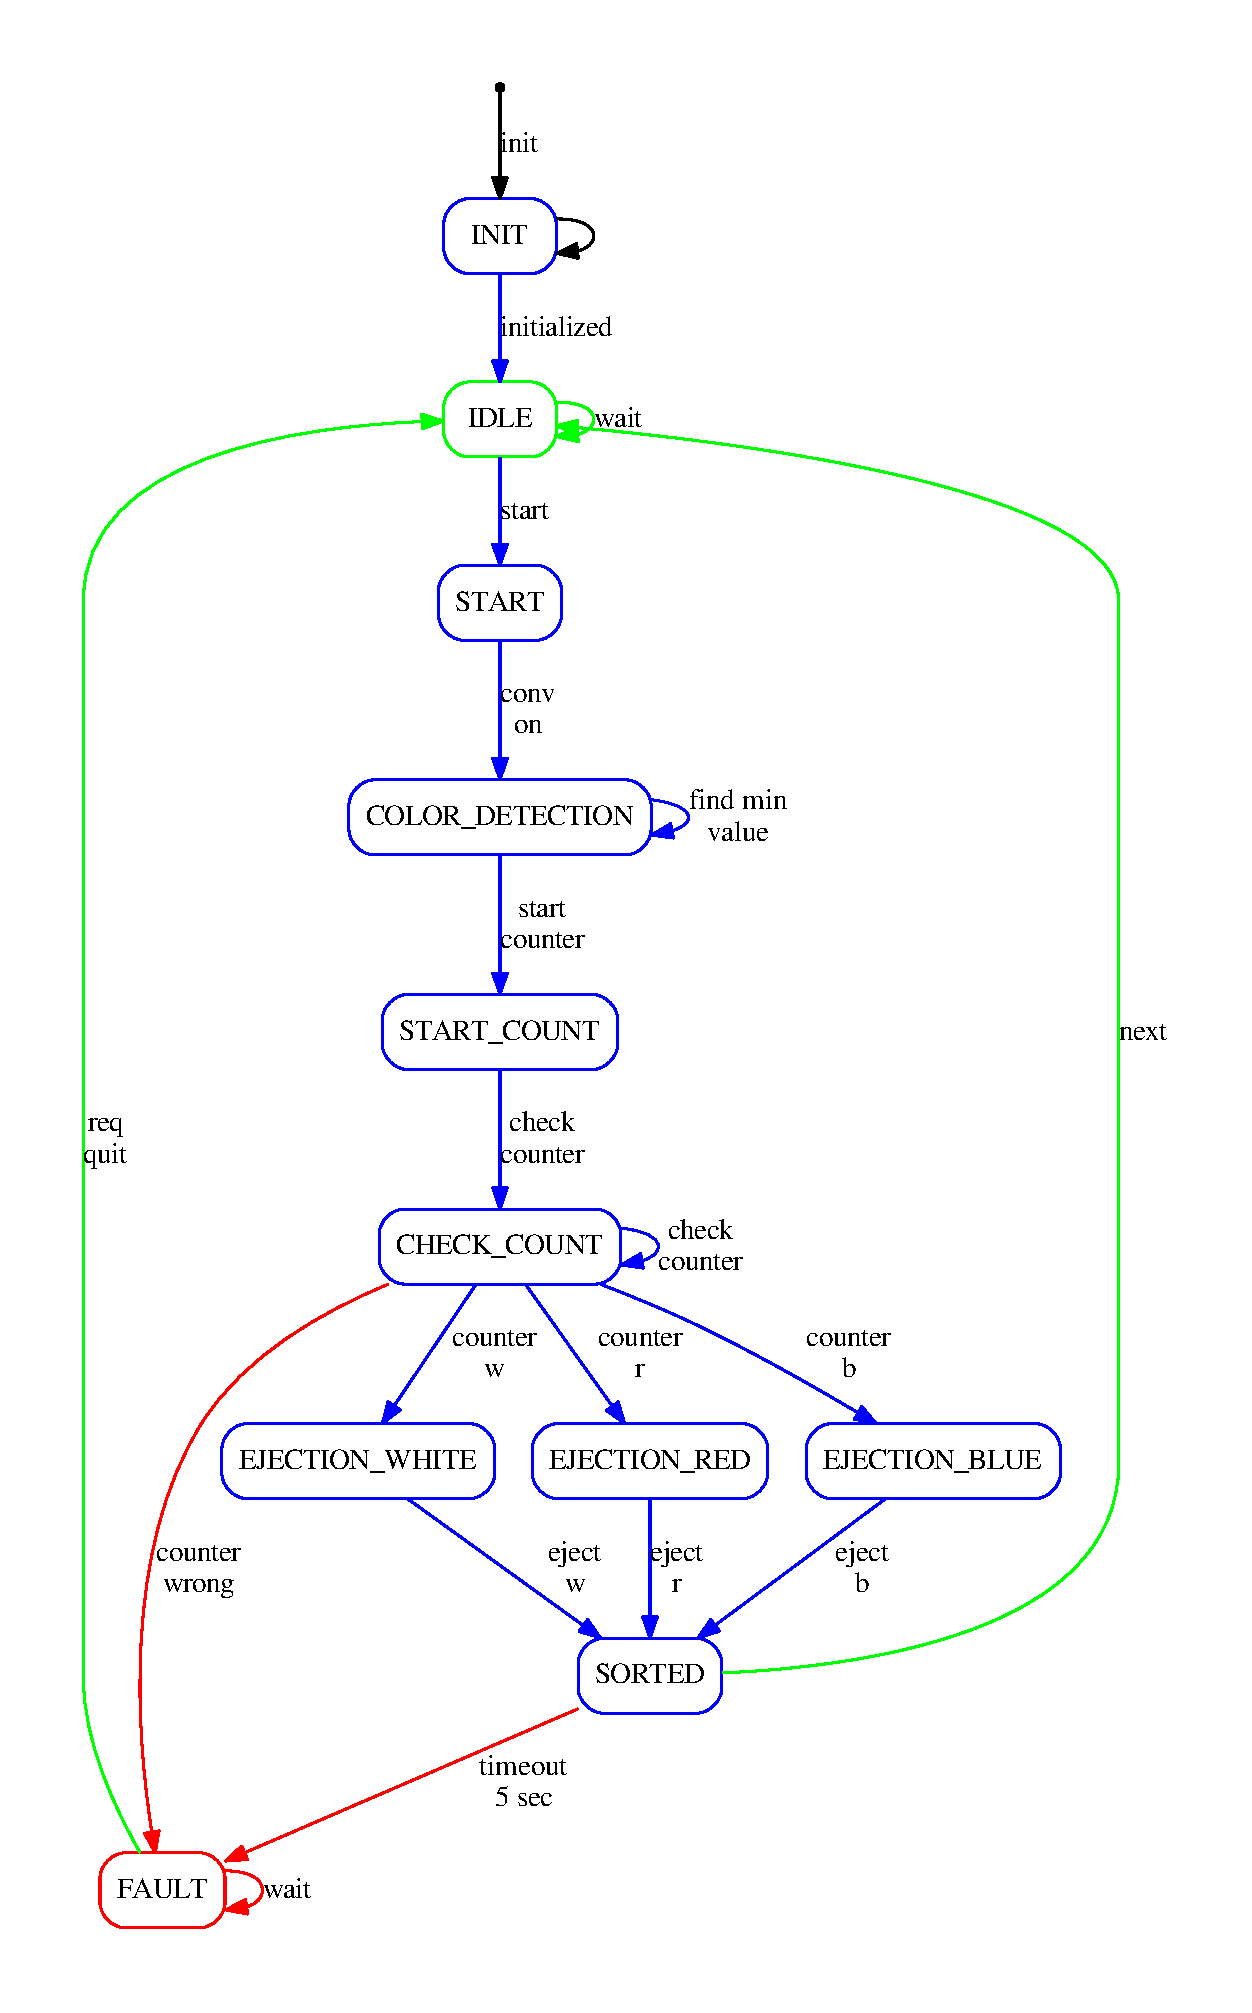
\includegraphics[width=\textwidth,height=\textheight/2,keepaspectratio=true]{dot_TxtSortingLineRun}}
\end{DoxyImageNoCaption}
\hypertarget{Overview State Machines_MPO}{}\section{Multi Processing Station}\label{Overview State Machines_MPO}

\begin{DoxyImageNoCaption}
  \mbox{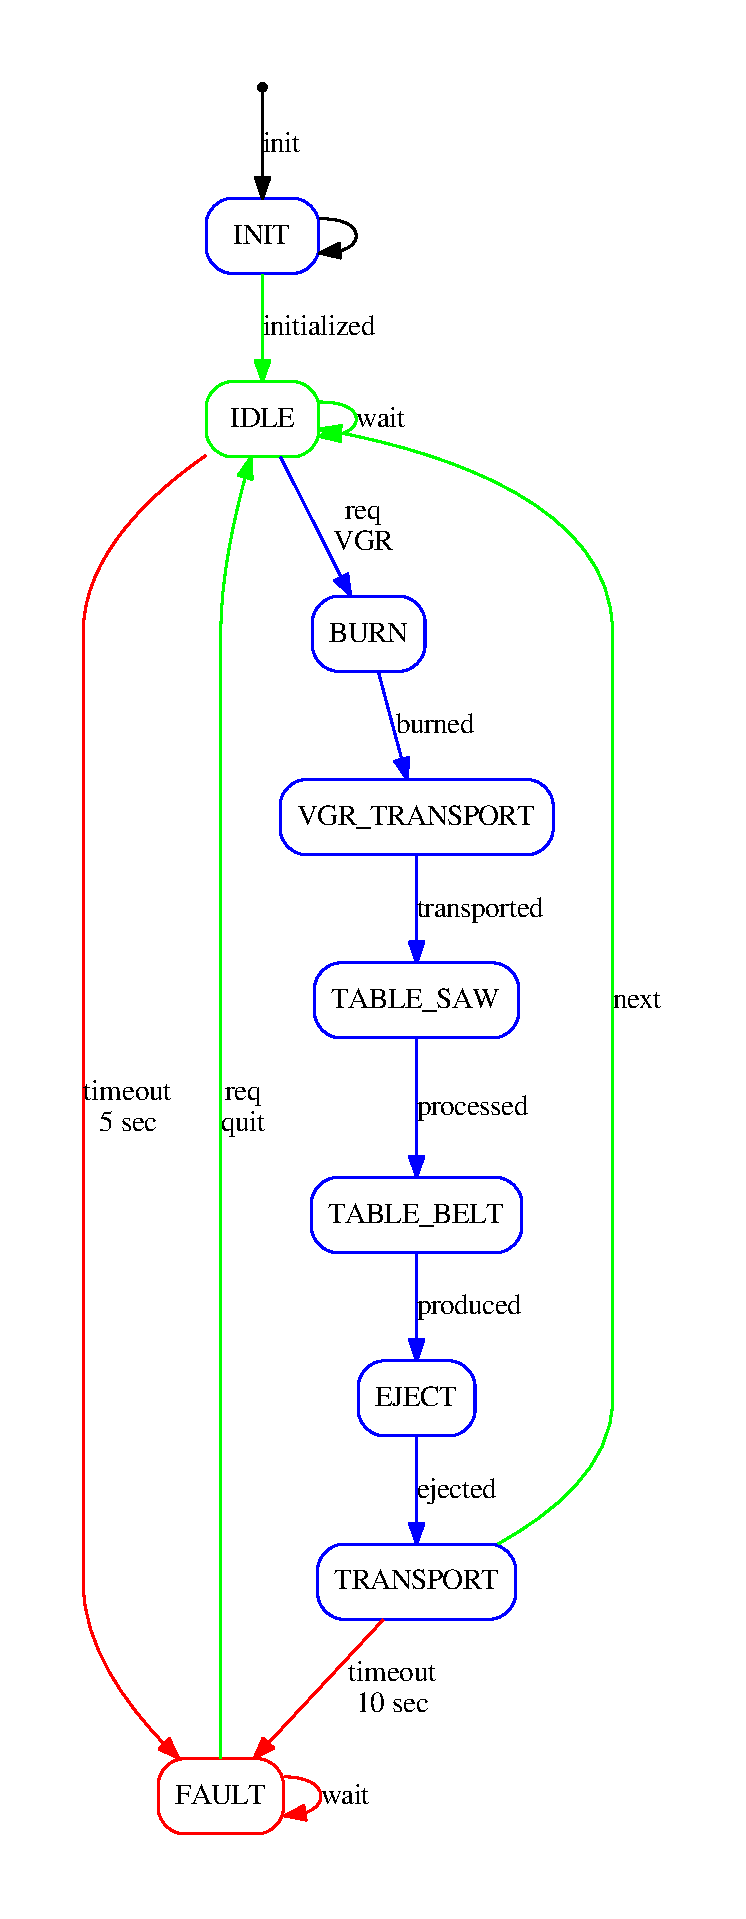
\includegraphics[width=\textwidth,height=\textheight/2,keepaspectratio=true]{dot_TxtMultiProcessingStationRun}}
\end{DoxyImageNoCaption}
\hypertarget{Overview State Machines_HBW}{}\section{High-\/\+Bay Warehouse}\label{Overview State Machines_HBW}

\begin{DoxyImageNoCaption}
  \mbox{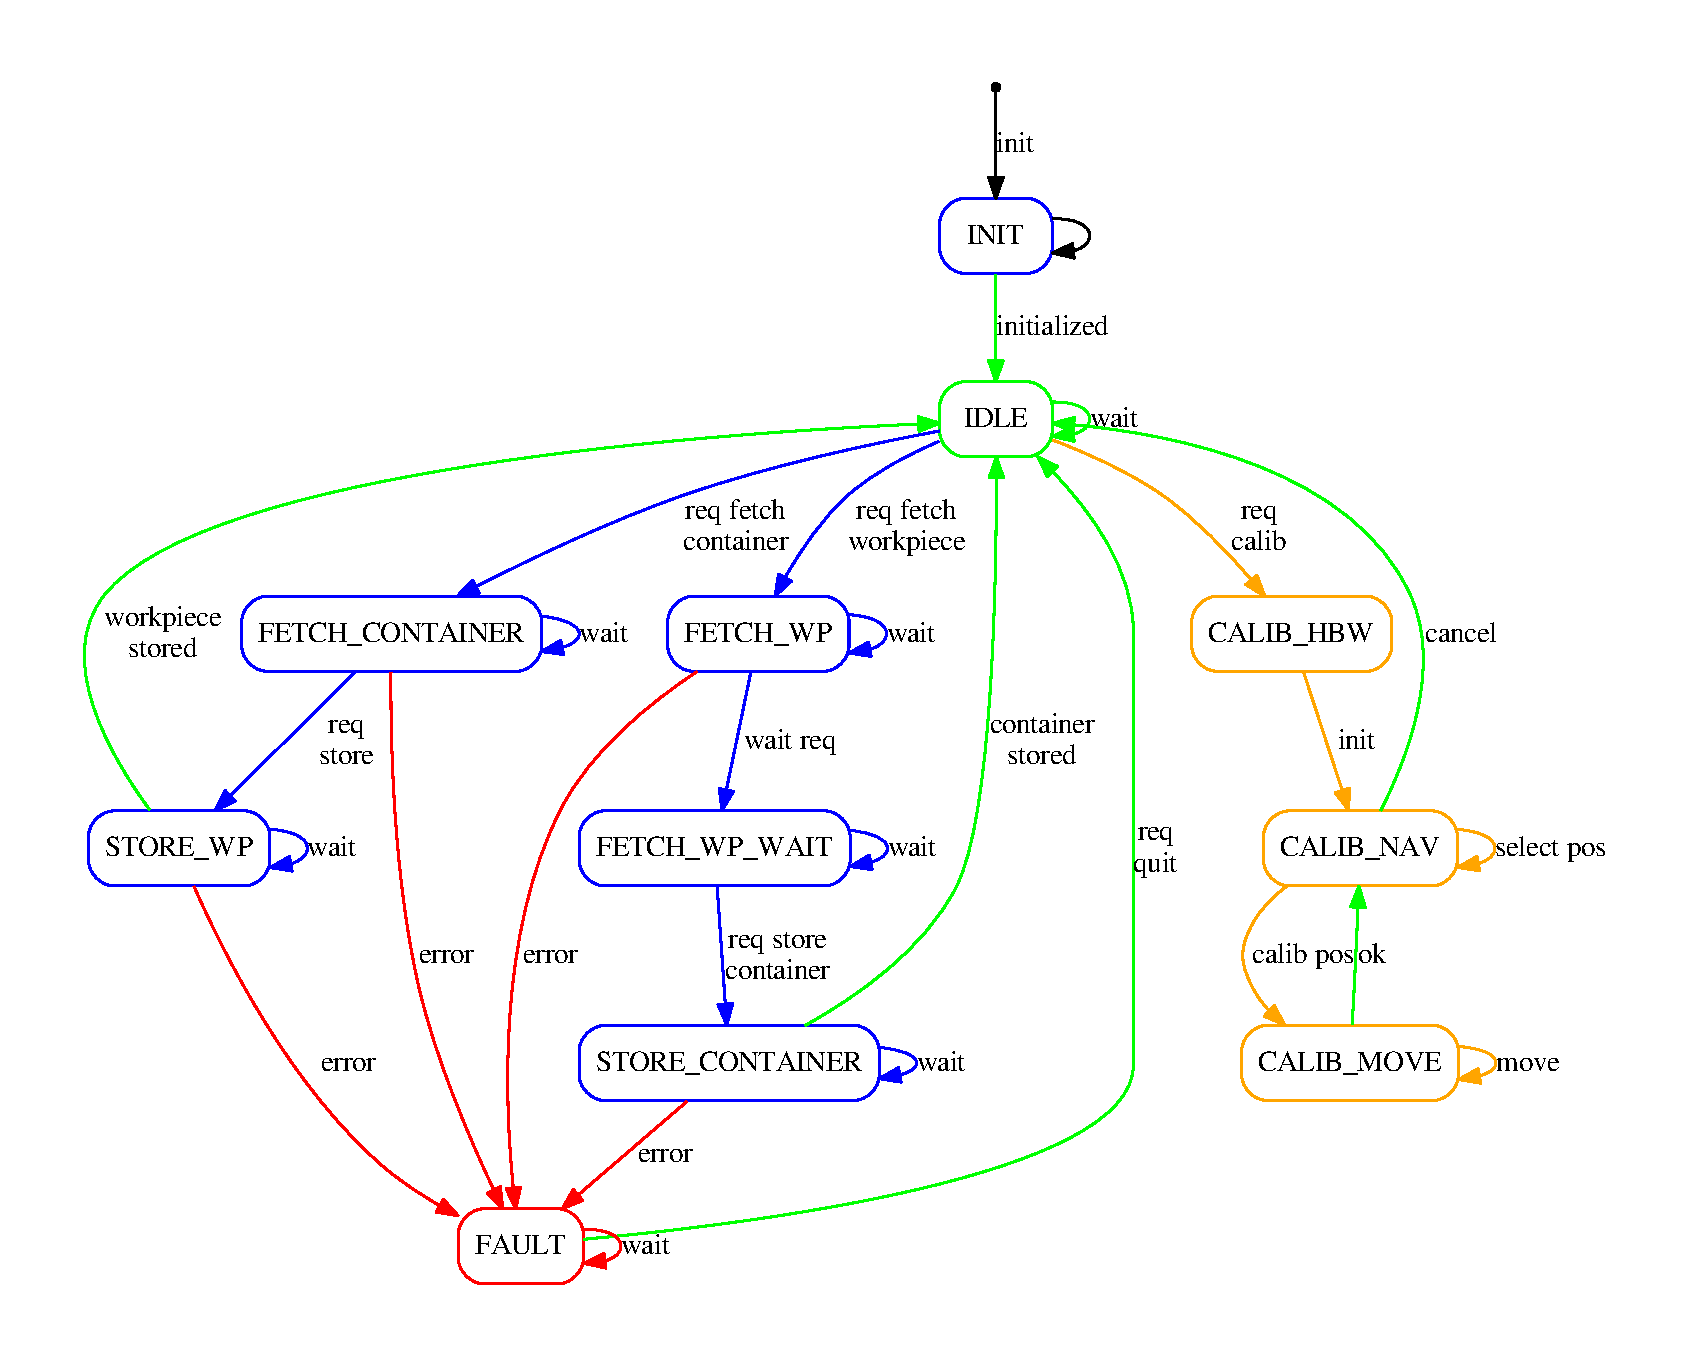
\includegraphics[width=\textwidth,height=\textheight/2,keepaspectratio=true]{dot_TxtHighBayWarehouseRun}}
\end{DoxyImageNoCaption}
\hypertarget{Overview State Machines_VGR}{}\section{Vacuum Gripper Robot}\label{Overview State Machines_VGR}

\begin{DoxyImageNoCaption}
  \mbox{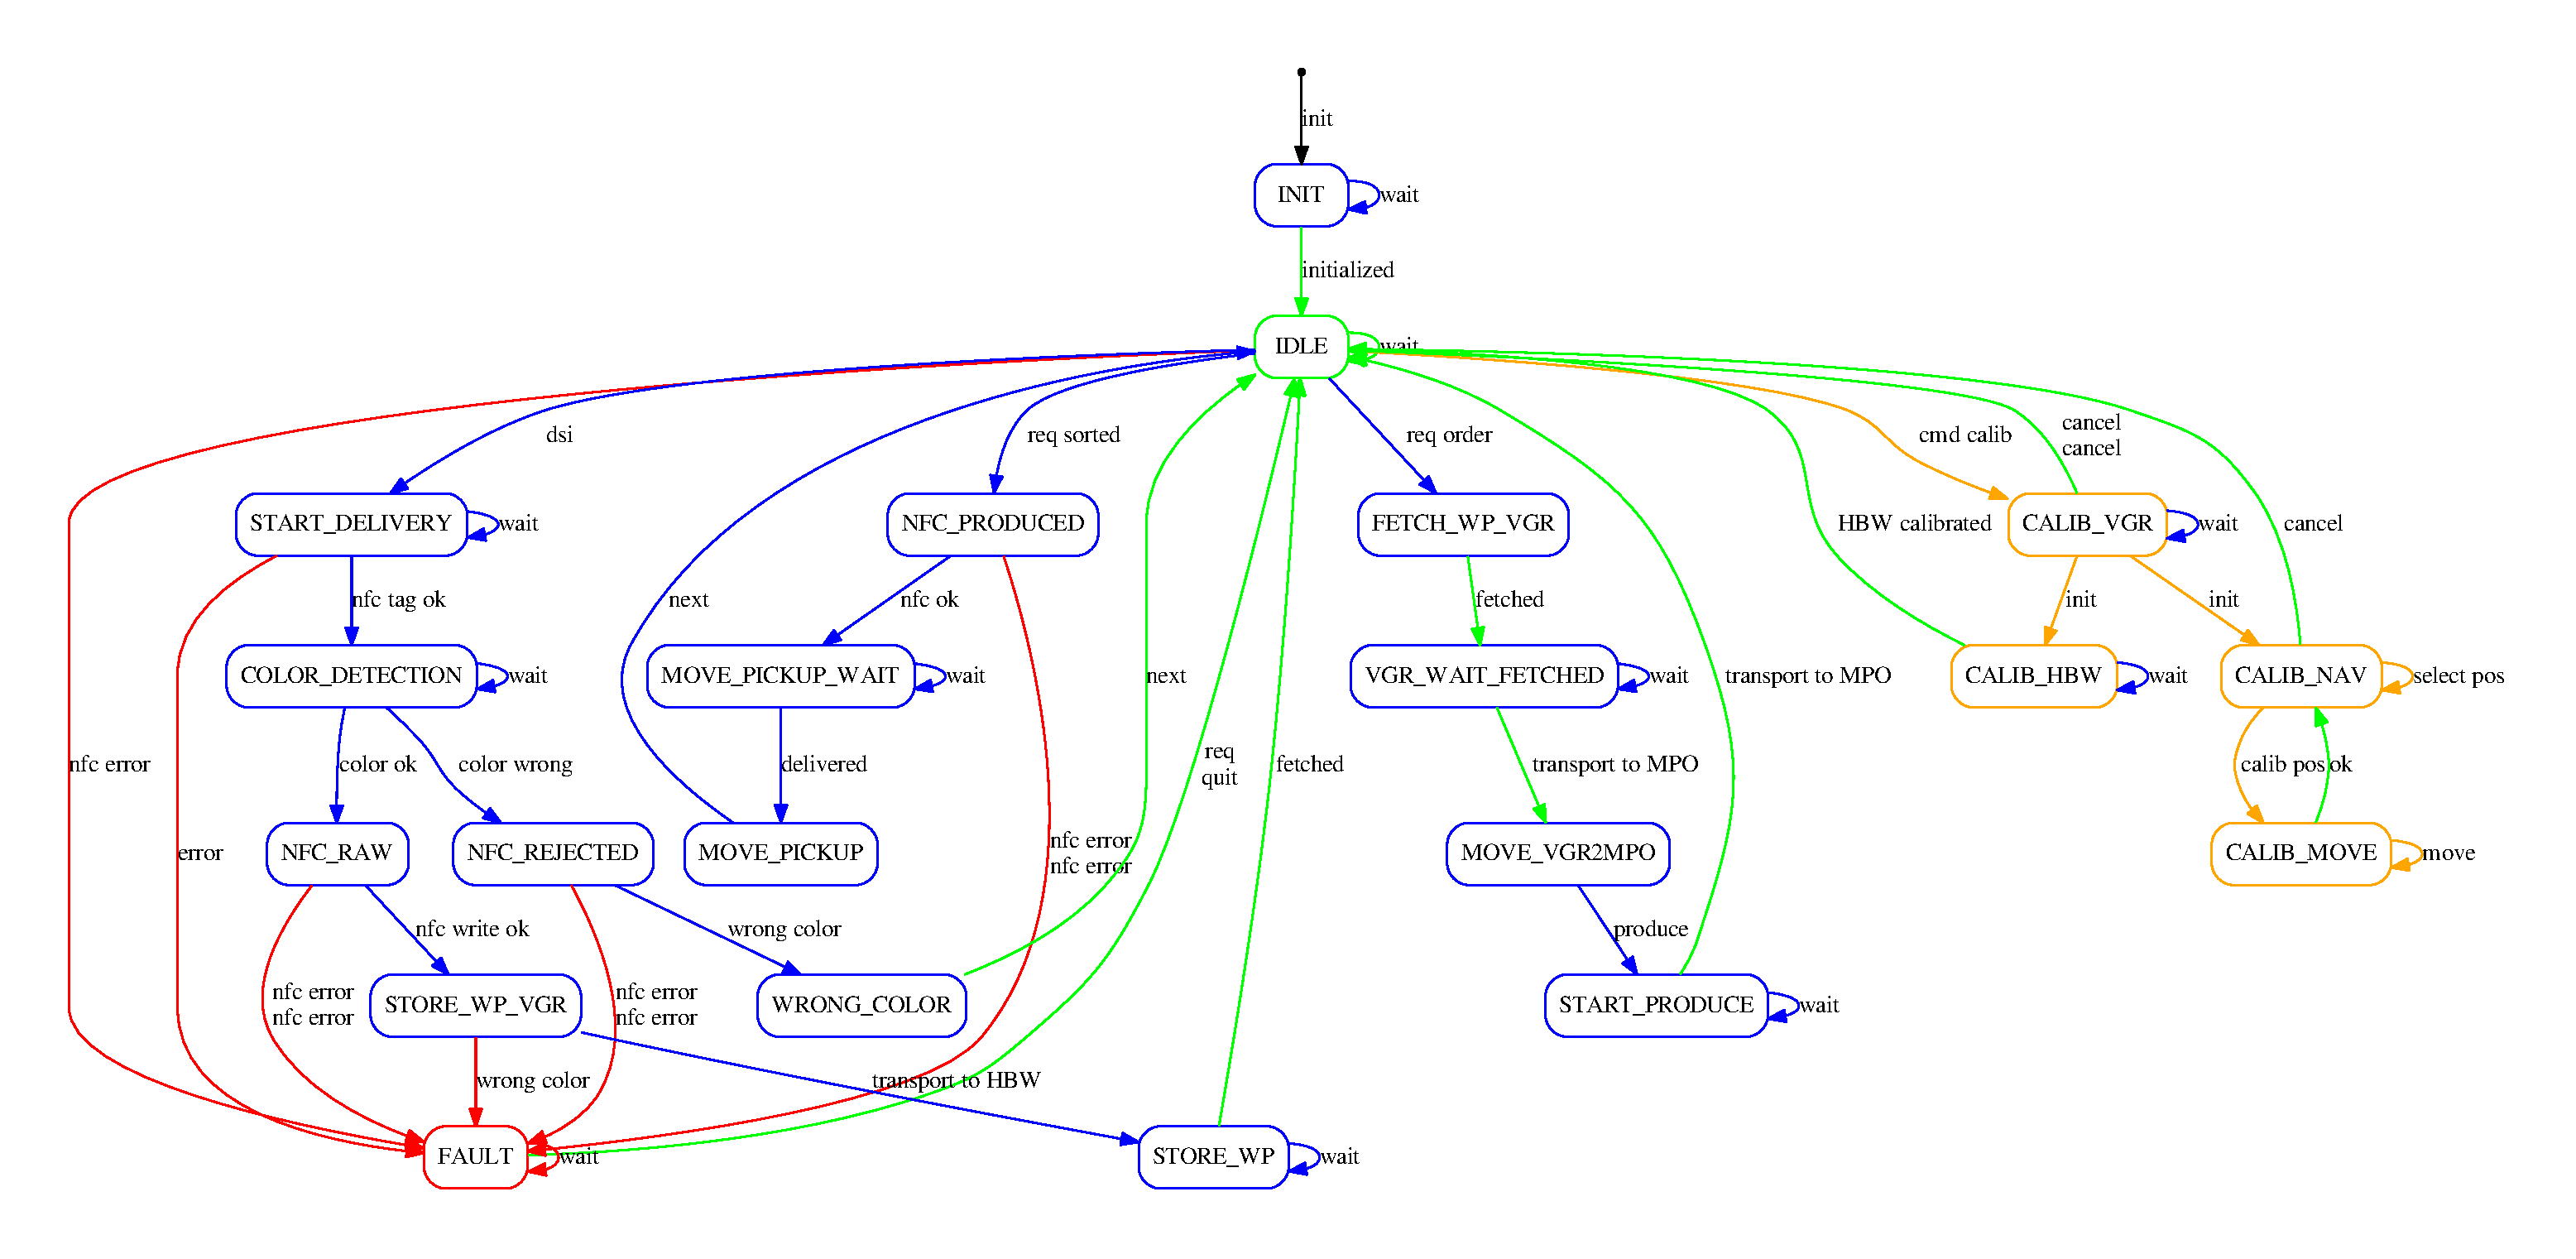
\includegraphics[width=\textwidth,height=\textheight/2,keepaspectratio=true]{dot_TxtVacuumGripperRobotRun}}
\end{DoxyImageNoCaption}
 
\chapter{Pin Assignment T\+XT controllers}
\label{md_PinAssignmentTXT}
\hypertarget{md_PinAssignmentTXT}{}
\section*{T\+XT 1\+: Sensor Station with Camera (S\+SC)}

\tabulinesep=1mm
\begin{longtabu} spread 0pt [c]{*2{|X[-1]}|}
\hline
\rowcolor{\tableheadbgcolor}\PBS\raggedleft {\bf T\+X\+T-\/\+IO }&{\bf Function  }\\\cline{1-2}
\endfirsthead
\hline
\endfoot
\hline
\rowcolor{\tableheadbgcolor}\PBS\raggedleft {\bf T\+X\+T-\/\+IO }&{\bf Function  }\\\cline{1-2}
\endhead
\PBS\raggedleft I1 &Reference Switch Pan \\\cline{1-2}
\PBS\raggedleft I2 &Reference Switch Tilt \\\cline{1-2}
\PBS\raggedleft I3 &Photoresistor \\\cline{1-2}
\PBS\raggedleft I4 &-\/ \\\cline{1-2}
\PBS\raggedleft I5 &Joystick X Front \\\cline{1-2}
\PBS\raggedleft I6 &Joystick Y Front \\\cline{1-2}
\PBS\raggedleft I7 &Joystick X Back \\\cline{1-2}
\PBS\raggedleft I8 &Joystick Y Back \\\cline{1-2}
\PBS\raggedleft C1 &Encoder Pan \\\cline{1-2}
\PBS\raggedleft C2 &Encoder Tilt \\\cline{1-2}
\PBS\raggedleft C3 &Joystick B Front \\\cline{1-2}
\PBS\raggedleft C4 &Joystick B Back \\\cline{1-2}
\PBS\raggedleft {\bfseries M1} &Motor Pan \\\cline{1-2}
\PBS\raggedleft {\bfseries M2} &Motor Tilt \\\cline{1-2}
\PBS\raggedleft {\bfseries O5} &L\+ED camera red \\\cline{1-2}
\PBS\raggedleft {\bfseries O6} &L\+ED lights red \\\cline{1-2}
\PBS\raggedleft {\bfseries O7} &L\+ED lights yellow \\\cline{1-2}
\PBS\raggedleft {\bfseries O8} &L\+ED lights green \\\cline{1-2}
\PBS\raggedleft {\itshape I2C} &{\itshape Environmental Sensor} \\\cline{1-2}
\end{longtabu}
\section*{T\+XT 2,3\+: Multi-\/\+Processing Station with Oven (M\+PO)}

\tabulinesep=1mm
\begin{longtabu} spread 0pt [c]{*2{|X[-1]}|}
\hline
\rowcolor{\tableheadbgcolor}\PBS\raggedleft {\bf T\+X\+T-\/\+IO }&{\bf Function  }\\\cline{1-2}
\endfirsthead
\hline
\endfoot
\hline
\rowcolor{\tableheadbgcolor}\PBS\raggedleft {\bf T\+X\+T-\/\+IO }&{\bf Function  }\\\cline{1-2}
\endhead
\PBS\raggedleft I1 (master) &Reference switch turn-\/table (position vacuum) \\\cline{1-2}
\PBS\raggedleft I2 (master) &Reference switch turn-\/table (position saw) \\\cline{1-2}
\PBS\raggedleft I3 (master) &Reference switch turn-\/table (position belt) \\\cline{1-2}
\PBS\raggedleft I4 (master) &Phototransistor end of conveyor belt \\\cline{1-2}
\PBS\raggedleft I5 (master) &Reference switch vacuum (position turn-\/table) \\\cline{1-2}
\PBS\raggedleft I6...I8 (master) &-\/ \\\cline{1-2}
\PBS\raggedleft C1...C4 (master) &-\/ \\\cline{1-2}
\PBS\raggedleft {\bfseries M1} (master) &Motor turn-\/table \\\cline{1-2}
\PBS\raggedleft {\bfseries M2} (master) &Motor saw \\\cline{1-2}
\PBS\raggedleft {\bfseries M3} (master) &Motor conveyor belt \\\cline{1-2}
\PBS\raggedleft {\bfseries O7} (master) &Valve ejection \\\cline{1-2}
\PBS\raggedleft {\bfseries O8} (master) &Compressor \\\cline{1-2}
\PBS\raggedleft {\itshape E\+XT (master)} &{\itshape T\+XT Extension} \\\cline{1-2}
\end{longtabu}
\tabulinesep=1mm
\begin{longtabu} spread 0pt [c]{*2{|X[-1]}|}
\hline
\rowcolor{\tableheadbgcolor}\PBS\raggedleft {\bf T\+X\+T-\/\+IO }&{\bf Function  }\\\cline{1-2}
\endfirsthead
\hline
\endfoot
\hline
\rowcolor{\tableheadbgcolor}\PBS\raggedleft {\bf T\+X\+T-\/\+IO }&{\bf Function  }\\\cline{1-2}
\endhead
\PBS\raggedleft I1 (extension) &Reference switch oven feeder retract \\\cline{1-2}
\PBS\raggedleft I2 (extension) &Reference switch oven feeder inside extend \\\cline{1-2}
\PBS\raggedleft I3 (extension) &Reference switch vacuum (position oven) \\\cline{1-2}
\PBS\raggedleft I4 (extension) &-\/ \\\cline{1-2}
\PBS\raggedleft I5 (extension) &Phototransistor \\\cline{1-2}
\PBS\raggedleft I6...I8 (extension) &-\/ \\\cline{1-2}
\PBS\raggedleft C1...C4 (extension) &-\/ \\\cline{1-2}
\PBS\raggedleft {\bfseries M1} (extension) &Motor oven feeder \\\cline{1-2}
\PBS\raggedleft {\bfseries M2} (extension) &Motor vacuum \\\cline{1-2}
\PBS\raggedleft {\bfseries O5} (extension) &Valve vacuum \\\cline{1-2}
\PBS\raggedleft {\bfseries O6} (extension) &Valve lowering \\\cline{1-2}
\PBS\raggedleft {\bfseries O7} (extension) &Valve oven door \\\cline{1-2}
\PBS\raggedleft {\bfseries O8} (extension) &Light oven \\\cline{1-2}
\PBS\raggedleft {\itshape E\+XT (extension)} &{\itshape T\+XT Master} \\\cline{1-2}
\end{longtabu}
\section*{T\+XT 4\+: High-\/\+Bay Warehouse (H\+BW)}

\tabulinesep=1mm
\begin{longtabu} spread 0pt [c]{*2{|X[-1]}|}
\hline
\rowcolor{\tableheadbgcolor}\PBS\raggedleft {\bf T\+X\+T-\/\+IO }&{\bf Function  }\\\cline{1-2}
\endfirsthead
\hline
\endfoot
\hline
\rowcolor{\tableheadbgcolor}\PBS\raggedleft {\bf T\+X\+T-\/\+IO }&{\bf Function  }\\\cline{1-2}
\endhead
\PBS\raggedleft I1 &Phototransistor Outside \\\cline{1-2}
\PBS\raggedleft I2...I3 &-\/ \\\cline{1-2}
\PBS\raggedleft I4 &Phototransistor Inside \\\cline{1-2}
\PBS\raggedleft I5 &Reference Switch horizontal axis \\\cline{1-2}
\PBS\raggedleft I6 &Reference Switch cantilever retract \\\cline{1-2}
\PBS\raggedleft I7 &Reference Switch cantilever extend \\\cline{1-2}
\PBS\raggedleft I8 &Reference Switch vertical axis \\\cline{1-2}
\PBS\raggedleft C1 &-\/ \\\cline{1-2}
\PBS\raggedleft C2 &Encoder horizontal axis \\\cline{1-2}
\PBS\raggedleft C3 &-\/ \\\cline{1-2}
\PBS\raggedleft C4 &Encoder vertical axis \\\cline{1-2}
\PBS\raggedleft {\bfseries M1} &Motor conveyor belt \\\cline{1-2}
\PBS\raggedleft {\bfseries M2} &Motor horizontal axis \\\cline{1-2}
\PBS\raggedleft {\bfseries M3} &Motor cantilever \\\cline{1-2}
\PBS\raggedleft {\bfseries M4} &Motor vertical axis \\\cline{1-2}
\end{longtabu}
\section*{T\+XT 5\+: Vacuum Gripper Robot (V\+GR), Delivery and Pickup Station (D\+PS)}

\tabulinesep=1mm
\begin{longtabu} spread 0pt [c]{*2{|X[-1]}|}
\hline
\rowcolor{\tableheadbgcolor}\PBS\raggedleft {\bf T\+X\+T-\/\+IO }&{\bf Function  }\\\cline{1-2}
\endfirsthead
\hline
\endfoot
\hline
\rowcolor{\tableheadbgcolor}\PBS\raggedleft {\bf T\+X\+T-\/\+IO }&{\bf Function  }\\\cline{1-2}
\endhead
\PBS\raggedleft I1 &Reference switch rotate \\\cline{1-2}
\PBS\raggedleft I2 &Reference switch vertical axis \\\cline{1-2}
\PBS\raggedleft I3 &Reference switch horizontal axis \\\cline{1-2}
\PBS\raggedleft I4...I6 &-\/ \\\cline{1-2}
\PBS\raggedleft I7 &Phototransistor Delivery (D\+PS) \\\cline{1-2}
\PBS\raggedleft I8 &Color Sensor (D\+PS) \\\cline{1-2}
\PBS\raggedleft C1 &Encoder rotate \\\cline{1-2}
\PBS\raggedleft C2 &Encoder vertical axis \\\cline{1-2}
\PBS\raggedleft C3 &Encoder horizontal axis \\\cline{1-2}
\PBS\raggedleft C4 &Phototransistor Pickup (D\+PS) \\\cline{1-2}
\PBS\raggedleft {\bfseries M1} &Motor rotate \\\cline{1-2}
\PBS\raggedleft {\bfseries M2} &Motor vertical axis \\\cline{1-2}
\PBS\raggedleft {\bfseries M3} &Motor horizontal axis \\\cline{1-2}
\PBS\raggedleft {\bfseries O7} &Compressor \\\cline{1-2}
\PBS\raggedleft {\bfseries O8} &Valve \\\cline{1-2}
\PBS\raggedleft {\itshape I2C} &{\itshape N\+F\+C/\+R\+F\+ID Module (D\+PS)} \\\cline{1-2}
\end{longtabu}
\section*{T\+XT 6\+: Sorting Line with Color Detection (S\+LD)}

\tabulinesep=1mm
\begin{longtabu} spread 0pt [c]{*2{|X[-1]}|}
\hline
\rowcolor{\tableheadbgcolor}\PBS\raggedleft {\bf T\+X\+T-\/\+IO }&{\bf Function  }\\\cline{1-2}
\endfirsthead
\hline
\endfoot
\hline
\rowcolor{\tableheadbgcolor}\PBS\raggedleft {\bf T\+X\+T-\/\+IO }&{\bf Function  }\\\cline{1-2}
\endhead
\PBS\raggedleft I1 &Phototransistor Color Sensor \\\cline{1-2}
\PBS\raggedleft I2 &Color Sensor \\\cline{1-2}
\PBS\raggedleft I3 &Phototransistor Ejection \\\cline{1-2}
\PBS\raggedleft I4...I5 &-\/ \\\cline{1-2}
\PBS\raggedleft I6 &Phototransistor White \\\cline{1-2}
\PBS\raggedleft I7 &Phototransistor Red \\\cline{1-2}
\PBS\raggedleft I8 &Phototransistor Blue \\\cline{1-2}
\PBS\raggedleft C1 &Pulse counter \\\cline{1-2}
\PBS\raggedleft C2...C4 &-\/ \\\cline{1-2}
\PBS\raggedleft {\bfseries M1} &Motor Conveyor Belt \\\cline{1-2}
\PBS\raggedleft {\bfseries M2} &-\/ \\\cline{1-2}
\PBS\raggedleft {\bfseries O5} &Valve Ejection White \\\cline{1-2}
\PBS\raggedleft {\bfseries O6} &Valve Ejection Red \\\cline{1-2}
\PBS\raggedleft {\bfseries O7} &Valve Ejection Blue \\\cline{1-2}
\PBS\raggedleft {\bfseries O8} &Compressor \\\cline{1-2}
\end{longtabu}

\chapter{M\+Q\+TT Interface}
\label{md_MqttInterface}
\hypertarget{md_MqttInterface}{}
\section*{M\+Q\+TT Remote (fichertechnik Cloud)}

\subsection*{fischertechnik Cloud / Dashboard}

\tabulinesep=1mm
\begin{longtabu} spread 0pt [c]{*2{|X[-1]}|}
\hline
\rowcolor{\tableheadbgcolor}\PBS\raggedleft {\bf Component }&{\bf topic S\+U\+B\+S\+C\+R\+I\+BE  }\\\cline{1-2}
\endfirsthead
\hline
\endfoot
\hline
\rowcolor{\tableheadbgcolor}\PBS\raggedleft {\bf Component }&{\bf topic S\+U\+B\+S\+C\+R\+I\+BE  }\\\cline{1-2}
\endhead
\PBS\raggedleft Environment Sensor &{\bfseries i/bme680} \\\cline{1-2}
\PBS\raggedleft Brightness Sensor &{\bfseries i/ldr} \\\cline{1-2}
\PBS\raggedleft Camera Picture &{\bfseries i/cam} \\\cline{1-2}
\PBS\raggedleft Pos Pan-\/\+Tilt-\/\+Unit &{\bfseries i/ptu/pos} \\\cline{1-2}
\PBS\raggedleft Alert Message &{\bfseries i/alert} \\\cline{1-2}
\PBS\raggedleft Broadcast &{\bfseries i/broadcast} \\\cline{1-2}
\PBS\raggedleft State H\+BW &{\bfseries f/i/state/hbw} \\\cline{1-2}
\PBS\raggedleft State V\+GR &{\bfseries f/i/state/vgr} \\\cline{1-2}
\PBS\raggedleft State M\+PO &{\bfseries f/i/state/mpo} \\\cline{1-2}
\PBS\raggedleft State S\+LD &{\bfseries f/i/state/sld} \\\cline{1-2}
\PBS\raggedleft State D\+SI (V\+GR) &{\bfseries f/i/state/dsi} \\\cline{1-2}
\PBS\raggedleft State D\+SO (V\+GR) &{\bfseries f/i/state/dso} \\\cline{1-2}
\PBS\raggedleft Stock H\+BW &{\bfseries f/i/stock} \\\cline{1-2}
\PBS\raggedleft State Order(\+V\+G\+R) &{\bfseries f/i/order} \\\cline{1-2}
\PBS\raggedleft State N\+FC Device (V\+GR) &{\bfseries f/i/nfc/ds} \\\cline{1-2}
\end{longtabu}
\tabulinesep=1mm
\begin{longtabu} spread 0pt [c]{*2{|X[-1]}|}
\hline
\rowcolor{\tableheadbgcolor}\PBS\raggedleft {\bf Component }&{\bf topic P\+U\+B\+L\+I\+SH  }\\\cline{1-2}
\endfirsthead
\hline
\endfoot
\hline
\rowcolor{\tableheadbgcolor}\PBS\raggedleft {\bf Component }&{\bf topic P\+U\+B\+L\+I\+SH  }\\\cline{1-2}
\endhead
\PBS\raggedleft T\+XT Pairing Ack &{\bfseries c/link} \\\cline{1-2}
\PBS\raggedleft Config Rate Environment Sensor &{\bfseries c/bme680} \\\cline{1-2}
\PBS\raggedleft Config Rate Brightness Sensor &{\bfseries c/ldr} \\\cline{1-2}
\PBS\raggedleft Config Rate Camera Picture &{\bfseries c/cam} \\\cline{1-2}
\PBS\raggedleft Control Buttons Pan-\/\+Tilt-\/\+Unit &{\bfseries o/ptu} \\\cline{1-2}
\PBS\raggedleft Quit Button &{\bfseries f/o/state/ack} \\\cline{1-2}
\PBS\raggedleft Order Workpiece Buttons &{\bfseries f/o/order} \\\cline{1-2}
\PBS\raggedleft Action Buttons N\+FC Module &{\bfseries f/o/nfc/ds} \\\cline{1-2}
\end{longtabu}
\section*{M\+Q\+TT Local}

\subsection*{Txt\+Factory\+Main}

\tabulinesep=1mm
\begin{longtabu} spread 0pt [c]{*2{|X[-1]}|}
\hline
\rowcolor{\tableheadbgcolor}\PBS\raggedleft {\bf Component }&{\bf topic S\+U\+B\+S\+C\+R\+I\+BE  }\\\cline{1-2}
\endfirsthead
\hline
\endfoot
\hline
\rowcolor{\tableheadbgcolor}\PBS\raggedleft {\bf Component }&{\bf topic S\+U\+B\+S\+C\+R\+I\+BE  }\\\cline{1-2}
\endhead
\PBS\raggedleft T\+XT Pairing Ack &{\bfseries c/link} \\\cline{1-2}
\PBS\raggedleft Config Rate Environment Sensor &{\bfseries c/bme680} \\\cline{1-2}
\PBS\raggedleft Config Rate Brightness Sensor &{\bfseries c/ldr} \\\cline{1-2}
\PBS\raggedleft Config Rate Camera Picture &{\bfseries c/cam} \\\cline{1-2}
\PBS\raggedleft Control Buttons Pan-\/\+Tilt-\/\+Unit &{\bfseries o/ptu} \\\cline{1-2}
\PBS\raggedleft Quit Button &{\bfseries f/o/state/ack} \\\cline{1-2}
\PBS\raggedleft State H\+BW &{\bfseries f/i/state/hbw} \\\cline{1-2}
\PBS\raggedleft State V\+GR &{\bfseries f/i/state/vgr} \\\cline{1-2}
\PBS\raggedleft State M\+PO &{\bfseries f/i/state/mpo} \\\cline{1-2}
\PBS\raggedleft State S\+LD &{\bfseries f/i/state/sld} \\\cline{1-2}
\PBS\raggedleft State D\+SI (V\+GR) &{\bfseries f/i/state/dsi} \\\cline{1-2}
\PBS\raggedleft State D\+SO (V\+GR) &{\bfseries f/i/state/dso} \\\cline{1-2}
\end{longtabu}
\tabulinesep=1mm
\begin{longtabu} spread 0pt [c]{*2{|X[-1]}|}
\hline
\rowcolor{\tableheadbgcolor}\PBS\raggedleft {\bf Components }&{\bf topic P\+U\+B\+L\+I\+SH  }\\\cline{1-2}
\endfirsthead
\hline
\endfoot
\hline
\rowcolor{\tableheadbgcolor}\PBS\raggedleft {\bf Components }&{\bf topic P\+U\+B\+L\+I\+SH  }\\\cline{1-2}
\endhead
\PBS\raggedleft Environment Sensor &{\bfseries i/bme680} \\\cline{1-2}
\PBS\raggedleft Brightness Sensor &{\bfseries i/ldr} \\\cline{1-2}
\PBS\raggedleft Camera Picture &{\bfseries i/cam} \\\cline{1-2}
\PBS\raggedleft Pos Pan-\/\+Tilt-\/\+Unit &{\bfseries i/ptu/pos} \\\cline{1-2}
\PBS\raggedleft Alert Message &{\bfseries i/alert} \\\cline{1-2}
\PBS\raggedleft Broadcast &{\bfseries i/broadcast} \\\cline{1-2}
\PBS\raggedleft Joysticks &{\bfseries fl/ssc/joy} \\\cline{1-2}
\end{longtabu}
\subsection*{Txt\+Factory\+M\+PO}

\tabulinesep=1mm
\begin{longtabu} spread 0pt [c]{*2{|X[-1]}|}
\hline
\rowcolor{\tableheadbgcolor}\PBS\raggedleft {\bf Components }&{\bf topic S\+U\+B\+S\+C\+R\+I\+BE  }\\\cline{1-2}
\endfirsthead
\hline
\endfoot
\hline
\rowcolor{\tableheadbgcolor}\PBS\raggedleft {\bf Components }&{\bf topic S\+U\+B\+S\+C\+R\+I\+BE  }\\\cline{1-2}
\endhead
\PBS\raggedleft Quit Button &{\bfseries f/o/state/ack} \\\cline{1-2}
\PBS\raggedleft V\+GR Trigger &{\bfseries fl/vgr/do} \\\cline{1-2}
\PBS\raggedleft Acknowledgment S\+LD &{\bfseries fl/sld/ack} \\\cline{1-2}
\end{longtabu}
\tabulinesep=1mm
\begin{longtabu} spread 0pt [c]{*2{|X[-1]}|}
\hline
\rowcolor{\tableheadbgcolor}\PBS\raggedleft {\bf Component }&{\bf topic P\+U\+B\+L\+I\+SH  }\\\cline{1-2}
\endfirsthead
\hline
\endfoot
\hline
\rowcolor{\tableheadbgcolor}\PBS\raggedleft {\bf Component }&{\bf topic P\+U\+B\+L\+I\+SH  }\\\cline{1-2}
\endhead
\PBS\raggedleft State M\+PO &{\bfseries f/i/state/mpo} \\\cline{1-2}
\PBS\raggedleft Acknowledgment M\+PO &{\bfseries fl/mpo/ack} \\\cline{1-2}
\end{longtabu}
\subsection*{Txt\+Factory\+H\+BW}

\tabulinesep=1mm
\begin{longtabu} spread 0pt [c]{*2{|X[-1]}|}
\hline
\rowcolor{\tableheadbgcolor}\PBS\raggedleft {\bf Component }&{\bf topic S\+U\+B\+S\+C\+R\+I\+BE  }\\\cline{1-2}
\endfirsthead
\hline
\endfoot
\hline
\rowcolor{\tableheadbgcolor}\PBS\raggedleft {\bf Component }&{\bf topic S\+U\+B\+S\+C\+R\+I\+BE  }\\\cline{1-2}
\endhead
\PBS\raggedleft Quit Button &{\bfseries f/o/state/ack} \\\cline{1-2}
\PBS\raggedleft Joysticks &{\bfseries fl/ssc/joy} \\\cline{1-2}
\PBS\raggedleft V\+GR Trigger &{\bfseries fl/vgr/do} \\\cline{1-2}
\end{longtabu}
\tabulinesep=1mm
\begin{longtabu} spread 0pt [c]{*2{|X[-1]}|}
\hline
\rowcolor{\tableheadbgcolor}\PBS\raggedleft {\bf Component }&{\bf topic P\+U\+B\+L\+I\+SH  }\\\cline{1-2}
\endfirsthead
\hline
\endfoot
\hline
\rowcolor{\tableheadbgcolor}\PBS\raggedleft {\bf Component }&{\bf topic P\+U\+B\+L\+I\+SH  }\\\cline{1-2}
\endhead
\PBS\raggedleft State H\+BW &{\bfseries f/i/state/hbw} \\\cline{1-2}
\PBS\raggedleft Acknowledgment H\+BW &{\bfseries fl/hbw/ack} \\\cline{1-2}
\end{longtabu}
\subsection*{Txt\+Factory\+V\+GR}

\tabulinesep=1mm
\begin{longtabu} spread 0pt [c]{*2{|X[-1]}|}
\hline
\rowcolor{\tableheadbgcolor}\PBS\raggedleft {\bf Component }&{\bf topic S\+U\+B\+S\+C\+R\+I\+BE  }\\\cline{1-2}
\endfirsthead
\hline
\endfoot
\hline
\rowcolor{\tableheadbgcolor}\PBS\raggedleft {\bf Component }&{\bf topic S\+U\+B\+S\+C\+R\+I\+BE  }\\\cline{1-2}
\endhead
\PBS\raggedleft Quit Button &{\bfseries f/o/state/ack} \\\cline{1-2}
\PBS\raggedleft Order Workpiece Buttons &{\bfseries f/o/order} \\\cline{1-2}
\PBS\raggedleft Action Buttons N\+FC Module &{\bfseries f/o/nfc/ds} \\\cline{1-2}
\PBS\raggedleft Joysticks &{\bfseries fl/ssc/joy} \\\cline{1-2}
\PBS\raggedleft Acknowledgment M\+PO &{\bfseries fl/mpo/ack} \\\cline{1-2}
\PBS\raggedleft Acknowledgment H\+BW &{\bfseries fl/hbw/ack} \\\cline{1-2}
\PBS\raggedleft Acknowledgment S\+LD &{\bfseries fl/sld/ack} \\\cline{1-2}
\end{longtabu}
\tabulinesep=1mm
\begin{longtabu} spread 0pt [c]{*2{|X[-1]}|}
\hline
\rowcolor{\tableheadbgcolor}\PBS\raggedleft {\bf Component }&{\bf topic P\+U\+B\+L\+I\+SH  }\\\cline{1-2}
\endfirsthead
\hline
\endfoot
\hline
\rowcolor{\tableheadbgcolor}\PBS\raggedleft {\bf Component }&{\bf topic P\+U\+B\+L\+I\+SH  }\\\cline{1-2}
\endhead
\PBS\raggedleft State V\+GR &{\bfseries f/i/state/vgr} \\\cline{1-2}
\PBS\raggedleft State D\+SI (V\+GR) &{\bfseries f/i/state/dsi} \\\cline{1-2}
\PBS\raggedleft State D\+SO (V\+GR) &{\bfseries f/i/state/dso} \\\cline{1-2}
\PBS\raggedleft V\+GR Trigger &{\bfseries fl/vgr/do} \\\cline{1-2}
\end{longtabu}
\subsection*{Txt\+Factory\+S\+LD}

\tabulinesep=1mm
\begin{longtabu} spread 0pt [c]{*2{|X[-1]}|}
\hline
\rowcolor{\tableheadbgcolor}\PBS\raggedleft {\bf Component }&{\bf topic S\+U\+B\+S\+C\+R\+I\+BE  }\\\cline{1-2}
\endfirsthead
\hline
\endfoot
\hline
\rowcolor{\tableheadbgcolor}\PBS\raggedleft {\bf Component }&{\bf topic S\+U\+B\+S\+C\+R\+I\+BE  }\\\cline{1-2}
\endhead
\PBS\raggedleft Quit Button &{\bfseries f/o/state/ack} \\\cline{1-2}
\PBS\raggedleft Acknowledgment M\+PO &{\bfseries fl/mpo/ack} \\\cline{1-2}
\end{longtabu}
\tabulinesep=1mm
\begin{longtabu} spread 0pt [c]{*2{|X[-1]}|}
\hline
\rowcolor{\tableheadbgcolor}\PBS\raggedleft {\bf Component }&{\bf topic P\+U\+B\+L\+I\+SH  }\\\cline{1-2}
\endfirsthead
\hline
\endfoot
\hline
\rowcolor{\tableheadbgcolor}\PBS\raggedleft {\bf Component }&{\bf topic P\+U\+B\+L\+I\+SH  }\\\cline{1-2}
\endhead
\PBS\raggedleft State S\+LD &{\bfseries f/i/state/sld} \\\cline{1-2}
\PBS\raggedleft Acknowledgment S\+LD &{\bfseries fl/sld/ack} \\\cline{1-2}
\end{longtabu}

\chapter{Dependencies}
\label{md_Dependencies}
\hypertarget{md_Dependencies}{}
\section*{External Libraries}


\begin{DoxyItemize}
\item paho-\/c \href{https://github.com/eclipse/paho.mqtt.c}{\tt https\+://github.\+com/eclipse/paho.\+mqtt.\+c}
\item paho-\/cpp \href{https://github.com/eclipse/paho.mqtt.cpp}{\tt https\+://github.\+com/eclipse/paho.\+mqtt.\+cpp}
\item jsoncpp \href{https://github.com/open-source-parsers/jsoncpp}{\tt https\+://github.\+com/open-\/source-\/parsers/jsoncpp}
\item opencv \href{https://github.com/opencv/opencv}{\tt https\+://github.\+com/opencv/opencv} \href{https://opencv.org/}{\tt https\+://opencv.\+org/}
\item libnfc \href{https://github.com/nfc-tools/libnfc}{\tt https\+://github.\+com/nfc-\/tools/libnfc}
\item libfreefare \href{https://github.com/nfc-tools/libfreefare}{\tt https\+://github.\+com/nfc-\/tools/libfreefare}
\item bme680\+\_\+driver \href{https://github.com/BoschSensortec/BME680_driver}{\tt https\+://github.\+com/\+Bosch\+Sensortec/\+B\+M\+E680\+\_\+driver}
\item algobsec \href{https://www.bosch-sensortec.com/bst/products/all_products/bsec}{\tt https\+://www.\+bosch-\/sensortec.\+com/bst/products/all\+\_\+products/bsec}
\item spdlog \href{https://github.com/gabime/spdlog}{\tt https\+://github.\+com/gabime/spdlog}
\end{DoxyItemize}

\section*{External Tools}


\begin{DoxyItemize}
\item Eclipse C\+DT \href{https://www.eclipse.org/cdt/}{\tt https\+://www.\+eclipse.\+org/cdt/}
\item Doxygen \href{http://www.doxygen.nl/}{\tt http\+://www.\+doxygen.\+nl/}
\item Graphviz \href{https://www.graphviz.org/}{\tt https\+://www.\+graphviz.\+org/}
\item Doc\+Fsm \href{https://github.com/UlrichBecker/DocFsm}{\tt https\+://github.\+com/\+Ulrich\+Becker/\+Doc\+Fsm} 
\end{DoxyItemize}
\chapter{Namespace Index}
\section{Namespace List}
Here is a list of all namespaces with brief descriptions\+:\begin{DoxyCompactList}
\item\contentsline{section}{\hyperlink{namespaceft}{ft} }{\pageref{namespaceft}}{}
\end{DoxyCompactList}

\chapter{Hierarchical Index}
\section{Class Hierarchy}
This inheritance list is sorted roughly, but not completely, alphabetically\+:\begin{DoxyCompactList}
\item \contentsline{section}{ft\+:\+:Bitset$<$ T $>$}{\pageref{structft_1_1_bitset}}{}
\item \contentsline{section}{ft\+:\+:Bitset$<$ unsigned long $>$}{\pageref{structft_1_1_bitset}}{}
\item \contentsline{section}{ft\+:\+:Enc\+Pos2}{\pageref{classft_1_1_enc_pos2}}{}
\item \contentsline{section}{ft\+:\+:Enc\+Pos3}{\pageref{classft_1_1_enc_pos3}}{}
\item iaction\+\_\+listener\begin{DoxyCompactList}
\item \contentsline{section}{ft\+:\+:action\+\_\+listener\+\_\+publish}{\pageref{classft_1_1action__listener__publish}}{}
\item \contentsline{section}{ft\+:\+:action\+\_\+listener\+\_\+subscribe}{\pageref{classft_1_1action__listener__subscribe}}{}
\end{DoxyCompactList}
\item \contentsline{section}{ft\+:\+:Observer}{\pageref{classft_1_1_observer}}{}
\begin{DoxyCompactList}
\item \contentsline{section}{ft\+:\+:Txt\+Delivery\+Pickup\+Station\+Observer}{\pageref{classft_1_1_txt_delivery_pickup_station_observer}}{}
\item \contentsline{section}{ft\+:\+:Txt\+High\+Bay\+Warehouse\+Observer}{\pageref{classft_1_1_txt_high_bay_warehouse_observer}}{}
\item \contentsline{section}{ft\+:\+:Txt\+High\+Bay\+Warehouse\+Storage\+Observer}{\pageref{classft_1_1_txt_high_bay_warehouse_storage_observer}}{}
\item \contentsline{section}{ft\+:\+:Txt\+Multi\+Processing\+Station\+Observer}{\pageref{classft_1_1_txt_multi_processing_station_observer}}{}
\item \contentsline{section}{ft\+:\+:Txt\+Nfc\+Device\+Observer}{\pageref{classft_1_1_txt_nfc_device_observer}}{}
\item \contentsline{section}{ft\+:\+:Txt\+Sorting\+Line\+Observer}{\pageref{classft_1_1_txt_sorting_line_observer}}{}
\item \contentsline{section}{ft\+:\+:Txt\+Vacuum\+Gripper\+Robot\+Observer}{\pageref{classft_1_1_txt_vacuum_gripper_robot_observer}}{}
\end{DoxyCompactList}
\item \contentsline{section}{ft\+:\+:Storage\+Pos2}{\pageref{structft_1_1_storage_pos2}}{}
\item \contentsline{section}{ft\+:\+:Subject\+Observer}{\pageref{classft_1_1_subject_observer}}{}
\begin{DoxyCompactList}
\item \contentsline{section}{ft\+:\+:Txt\+Axis}{\pageref{classft_1_1_txt_axis}}{}
\begin{DoxyCompactList}
\item \contentsline{section}{ft\+:\+:Txt\+Axis1\+Ref\+Switch}{\pageref{classft_1_1_txt_axis1_ref_switch}}{}
\item \contentsline{section}{ft\+:\+:Txt\+Axis\+N\+Ref\+Switch}{\pageref{classft_1_1_txt_axis_n_ref_switch}}{}
\end{DoxyCompactList}
\item \contentsline{section}{ft\+:\+:Txt\+B\+M\+E680}{\pageref{classft_1_1_txt_b_m_e680}}{}
\item \contentsline{section}{ft\+:\+:Txt\+Camera}{\pageref{classft_1_1_txt_camera}}{}
\item \contentsline{section}{ft\+:\+:Txt\+High\+Bay\+Warehouse\+Storage}{\pageref{classft_1_1_txt_high_bay_warehouse_storage}}{}
\item \contentsline{section}{ft\+:\+:Txt\+Joystick\+X\+Y\+B\+Controller}{\pageref{classft_1_1_txt_joystick_x_y_b_controller}}{}
\item \contentsline{section}{ft\+:\+:Txt\+Motion\+Detection}{\pageref{classft_1_1_txt_motion_detection}}{}
\item \contentsline{section}{ft\+:\+:Txt\+Nfc\+Device}{\pageref{classft_1_1_txt_nfc_device}}{}
\item \contentsline{section}{ft\+:\+:Txt\+Pan\+Tilt\+Unit}{\pageref{classft_1_1_txt_pan_tilt_unit}}{}
\item \contentsline{section}{ft\+:\+:Txt\+Simulation\+Model}{\pageref{classft_1_1_txt_simulation_model}}{}
\begin{DoxyCompactList}
\item \contentsline{section}{ft\+:\+:Txt\+Delivery\+Pickup\+Station}{\pageref{classft_1_1_txt_delivery_pickup_station}}{}
\item \contentsline{section}{ft\+:\+:Txt\+High\+Bay\+Warehouse}{\pageref{classft_1_1_txt_high_bay_warehouse}}{}
\item \contentsline{section}{ft\+:\+:Txt\+Multi\+Processing\+Station}{\pageref{classft_1_1_txt_multi_processing_station}}{}
\item \contentsline{section}{ft\+:\+:Txt\+Sorting\+Line}{\pageref{classft_1_1_txt_sorting_line}}{}
\item \contentsline{section}{ft\+:\+:Txt\+Vacuum\+Gripper\+Robot}{\pageref{classft_1_1_txt_vacuum_gripper_robot}}{}
\end{DoxyCompactList}
\end{DoxyCompactList}
\item \contentsline{section}{ft\+:\+:ts\+\_\+u}{\pageref{unionft_1_1ts__u}}{}
\item \contentsline{section}{ft\+:\+:Txt\+Calib\+Data}{\pageref{classft_1_1_txt_calib_data}}{}
\begin{DoxyCompactList}
\item \contentsline{section}{ft\+:\+:Txt\+Delivery\+Pickup\+Station\+Calib\+Data}{\pageref{classft_1_1_txt_delivery_pickup_station_calib_data}}{}
\item \contentsline{section}{ft\+:\+:Txt\+High\+Bay\+Warehouse\+Calib\+Data}{\pageref{classft_1_1_txt_high_bay_warehouse_calib_data}}{}
\item \contentsline{section}{ft\+:\+:Txt\+Pan\+Tilt\+Unit\+Calib\+Data}{\pageref{classft_1_1_txt_pan_tilt_unit_calib_data}}{}
\item \contentsline{section}{ft\+:\+:Txt\+Sorting\+Line\+Calib\+Data}{\pageref{classft_1_1_txt_sorting_line_calib_data}}{}
\item \contentsline{section}{ft\+:\+:Txt\+Vacuum\+Gripper\+Robot\+Calib\+Data}{\pageref{classft_1_1_txt_vacuum_gripper_robot_calib_data}}{}
\end{DoxyCompactList}
\item \contentsline{section}{ft\+:\+:Txt\+Conveyor\+Belt}{\pageref{classft_1_1_txt_conveyor_belt}}{}
\begin{DoxyCompactList}
\item \contentsline{section}{ft\+:\+:Txt\+Conveyor\+Belt\+Light\+Barriers}{\pageref{classft_1_1_txt_conveyor_belt_light_barriers}}{}
\end{DoxyCompactList}
\item \contentsline{section}{ft\+:\+:Txt\+Factory\+Process\+Storage}{\pageref{classft_1_1_txt_factory_process_storage}}{}
\item \contentsline{section}{ft\+:\+:Txt\+Flapping}{\pageref{classft_1_1_txt_flapping}}{}
\item \contentsline{section}{ft\+:\+:Txt\+Joysticks\+Data}{\pageref{classft_1_1_txt_joysticks_data}}{}
\item \contentsline{section}{ft\+:\+:Txt\+Mqtt\+Factory\+Client}{\pageref{classft_1_1_txt_mqtt_factory_client}}{}
\item \contentsline{section}{ft\+:\+:Txt\+Nfc\+Data}{\pageref{classft_1_1_txt_nfc_data}}{}
\item \contentsline{section}{ft\+:\+:Txt\+Order\+State}{\pageref{structft_1_1_txt_order_state}}{}
\item \contentsline{section}{ft\+:\+:Txt\+Pan\+Tilt\+Unit\+Controller}{\pageref{classft_1_1_txt_pan_tilt_unit_controller}}{}
\item \contentsline{section}{ft\+:\+:Txt\+Vacuum\+Gripper}{\pageref{classft_1_1_txt_vacuum_gripper}}{}
\item \contentsline{section}{ft\+:\+:Txt\+Workpiece}{\pageref{classft_1_1_txt_workpiece}}{}
\end{DoxyCompactList}

\chapter{Class Index}
\section{Class List}
Here are the classes, structs, unions and interfaces with brief descriptions\+:\begin{DoxyCompactList}
\item\contentsline{section}{\hyperlink{classft_1_1action__listener__publish}{ft\+::action\+\_\+listener\+\_\+publish} }{\pageref{classft_1_1action__listener__publish}}{}
\item\contentsline{section}{\hyperlink{classft_1_1action__listener__subscribe}{ft\+::action\+\_\+listener\+\_\+subscribe} }{\pageref{classft_1_1action__listener__subscribe}}{}
\item\contentsline{section}{\hyperlink{structft_1_1_bitset}{ft\+::\+Bitset$<$ T $>$} }{\pageref{structft_1_1_bitset}}{}
\item\contentsline{section}{\hyperlink{classft_1_1_enc_pos2}{ft\+::\+Enc\+Pos2} }{\pageref{classft_1_1_enc_pos2}}{}
\item\contentsline{section}{\hyperlink{classft_1_1_enc_pos3}{ft\+::\+Enc\+Pos3} }{\pageref{classft_1_1_enc_pos3}}{}
\item\contentsline{section}{\hyperlink{classft_1_1_observer}{ft\+::\+Observer} }{\pageref{classft_1_1_observer}}{}
\item\contentsline{section}{\hyperlink{structft_1_1_storage_pos2}{ft\+::\+Storage\+Pos2} }{\pageref{structft_1_1_storage_pos2}}{}
\item\contentsline{section}{\hyperlink{classft_1_1_subject_observer}{ft\+::\+Subject\+Observer} }{\pageref{classft_1_1_subject_observer}}{}
\item\contentsline{section}{\hyperlink{unionft_1_1ts__u}{ft\+::ts\+\_\+u} }{\pageref{unionft_1_1ts__u}}{}
\item\contentsline{section}{\hyperlink{classft_1_1_txt_axis}{ft\+::\+Txt\+Axis} }{\pageref{classft_1_1_txt_axis}}{}
\item\contentsline{section}{\hyperlink{classft_1_1_txt_axis1_ref_switch}{ft\+::\+Txt\+Axis1\+Ref\+Switch} }{\pageref{classft_1_1_txt_axis1_ref_switch}}{}
\item\contentsline{section}{\hyperlink{classft_1_1_txt_axis_n_ref_switch}{ft\+::\+Txt\+Axis\+N\+Ref\+Switch} }{\pageref{classft_1_1_txt_axis_n_ref_switch}}{}
\item\contentsline{section}{\hyperlink{classft_1_1_txt_b_m_e680}{ft\+::\+Txt\+B\+M\+E680} }{\pageref{classft_1_1_txt_b_m_e680}}{}
\item\contentsline{section}{\hyperlink{classft_1_1_txt_calib_data}{ft\+::\+Txt\+Calib\+Data} }{\pageref{classft_1_1_txt_calib_data}}{}
\item\contentsline{section}{\hyperlink{classft_1_1_txt_camera}{ft\+::\+Txt\+Camera} }{\pageref{classft_1_1_txt_camera}}{}
\item\contentsline{section}{\hyperlink{classft_1_1_txt_conveyor_belt}{ft\+::\+Txt\+Conveyor\+Belt} }{\pageref{classft_1_1_txt_conveyor_belt}}{}
\item\contentsline{section}{\hyperlink{classft_1_1_txt_conveyor_belt_light_barriers}{ft\+::\+Txt\+Conveyor\+Belt\+Light\+Barriers} }{\pageref{classft_1_1_txt_conveyor_belt_light_barriers}}{}
\item\contentsline{section}{\hyperlink{classft_1_1_txt_delivery_pickup_station}{ft\+::\+Txt\+Delivery\+Pickup\+Station} }{\pageref{classft_1_1_txt_delivery_pickup_station}}{}
\item\contentsline{section}{\hyperlink{classft_1_1_txt_delivery_pickup_station_calib_data}{ft\+::\+Txt\+Delivery\+Pickup\+Station\+Calib\+Data} }{\pageref{classft_1_1_txt_delivery_pickup_station_calib_data}}{}
\item\contentsline{section}{\hyperlink{classft_1_1_txt_delivery_pickup_station_observer}{ft\+::\+Txt\+Delivery\+Pickup\+Station\+Observer} }{\pageref{classft_1_1_txt_delivery_pickup_station_observer}}{}
\item\contentsline{section}{\hyperlink{classft_1_1_txt_factory_process_storage}{ft\+::\+Txt\+Factory\+Process\+Storage} }{\pageref{classft_1_1_txt_factory_process_storage}}{}
\item\contentsline{section}{\hyperlink{classft_1_1_txt_flapping}{ft\+::\+Txt\+Flapping} }{\pageref{classft_1_1_txt_flapping}}{}
\item\contentsline{section}{\hyperlink{classft_1_1_txt_high_bay_warehouse}{ft\+::\+Txt\+High\+Bay\+Warehouse} }{\pageref{classft_1_1_txt_high_bay_warehouse}}{}
\item\contentsline{section}{\hyperlink{classft_1_1_txt_high_bay_warehouse_calib_data}{ft\+::\+Txt\+High\+Bay\+Warehouse\+Calib\+Data} }{\pageref{classft_1_1_txt_high_bay_warehouse_calib_data}}{}
\item\contentsline{section}{\hyperlink{classft_1_1_txt_high_bay_warehouse_observer}{ft\+::\+Txt\+High\+Bay\+Warehouse\+Observer} }{\pageref{classft_1_1_txt_high_bay_warehouse_observer}}{}
\item\contentsline{section}{\hyperlink{classft_1_1_txt_high_bay_warehouse_storage}{ft\+::\+Txt\+High\+Bay\+Warehouse\+Storage} }{\pageref{classft_1_1_txt_high_bay_warehouse_storage}}{}
\item\contentsline{section}{\hyperlink{classft_1_1_txt_high_bay_warehouse_storage_observer}{ft\+::\+Txt\+High\+Bay\+Warehouse\+Storage\+Observer} }{\pageref{classft_1_1_txt_high_bay_warehouse_storage_observer}}{}
\item\contentsline{section}{\hyperlink{classft_1_1_txt_joysticks_data}{ft\+::\+Txt\+Joysticks\+Data} }{\pageref{classft_1_1_txt_joysticks_data}}{}
\item\contentsline{section}{\hyperlink{classft_1_1_txt_joystick_x_y_b_controller}{ft\+::\+Txt\+Joystick\+X\+Y\+B\+Controller} }{\pageref{classft_1_1_txt_joystick_x_y_b_controller}}{}
\item\contentsline{section}{\hyperlink{classft_1_1_txt_motion_detection}{ft\+::\+Txt\+Motion\+Detection} }{\pageref{classft_1_1_txt_motion_detection}}{}
\item\contentsline{section}{\hyperlink{classft_1_1_txt_mqtt_factory_client}{ft\+::\+Txt\+Mqtt\+Factory\+Client} }{\pageref{classft_1_1_txt_mqtt_factory_client}}{}
\item\contentsline{section}{\hyperlink{classft_1_1_txt_multi_processing_station}{ft\+::\+Txt\+Multi\+Processing\+Station} }{\pageref{classft_1_1_txt_multi_processing_station}}{}
\item\contentsline{section}{\hyperlink{classft_1_1_txt_multi_processing_station_observer}{ft\+::\+Txt\+Multi\+Processing\+Station\+Observer} }{\pageref{classft_1_1_txt_multi_processing_station_observer}}{}
\item\contentsline{section}{\hyperlink{classft_1_1_txt_nfc_data}{ft\+::\+Txt\+Nfc\+Data} }{\pageref{classft_1_1_txt_nfc_data}}{}
\item\contentsline{section}{\hyperlink{classft_1_1_txt_nfc_device}{ft\+::\+Txt\+Nfc\+Device} }{\pageref{classft_1_1_txt_nfc_device}}{}
\item\contentsline{section}{\hyperlink{classft_1_1_txt_nfc_device_observer}{ft\+::\+Txt\+Nfc\+Device\+Observer} }{\pageref{classft_1_1_txt_nfc_device_observer}}{}
\item\contentsline{section}{\hyperlink{structft_1_1_txt_order_state}{ft\+::\+Txt\+Order\+State} }{\pageref{structft_1_1_txt_order_state}}{}
\item\contentsline{section}{\hyperlink{classft_1_1_txt_pan_tilt_unit}{ft\+::\+Txt\+Pan\+Tilt\+Unit} }{\pageref{classft_1_1_txt_pan_tilt_unit}}{}
\item\contentsline{section}{\hyperlink{classft_1_1_txt_pan_tilt_unit_calib_data}{ft\+::\+Txt\+Pan\+Tilt\+Unit\+Calib\+Data} }{\pageref{classft_1_1_txt_pan_tilt_unit_calib_data}}{}
\item\contentsline{section}{\hyperlink{classft_1_1_txt_pan_tilt_unit_controller}{ft\+::\+Txt\+Pan\+Tilt\+Unit\+Controller} }{\pageref{classft_1_1_txt_pan_tilt_unit_controller}}{}
\item\contentsline{section}{\hyperlink{classft_1_1_txt_simulation_model}{ft\+::\+Txt\+Simulation\+Model} }{\pageref{classft_1_1_txt_simulation_model}}{}
\item\contentsline{section}{\hyperlink{classft_1_1_txt_sorting_line}{ft\+::\+Txt\+Sorting\+Line} }{\pageref{classft_1_1_txt_sorting_line}}{}
\item\contentsline{section}{\hyperlink{classft_1_1_txt_sorting_line_calib_data}{ft\+::\+Txt\+Sorting\+Line\+Calib\+Data} }{\pageref{classft_1_1_txt_sorting_line_calib_data}}{}
\item\contentsline{section}{\hyperlink{classft_1_1_txt_sorting_line_observer}{ft\+::\+Txt\+Sorting\+Line\+Observer} }{\pageref{classft_1_1_txt_sorting_line_observer}}{}
\item\contentsline{section}{\hyperlink{classft_1_1_txt_vacuum_gripper}{ft\+::\+Txt\+Vacuum\+Gripper} }{\pageref{classft_1_1_txt_vacuum_gripper}}{}
\item\contentsline{section}{\hyperlink{classft_1_1_txt_vacuum_gripper_robot}{ft\+::\+Txt\+Vacuum\+Gripper\+Robot} }{\pageref{classft_1_1_txt_vacuum_gripper_robot}}{}
\item\contentsline{section}{\hyperlink{classft_1_1_txt_vacuum_gripper_robot_calib_data}{ft\+::\+Txt\+Vacuum\+Gripper\+Robot\+Calib\+Data} }{\pageref{classft_1_1_txt_vacuum_gripper_robot_calib_data}}{}
\item\contentsline{section}{\hyperlink{classft_1_1_txt_vacuum_gripper_robot_observer}{ft\+::\+Txt\+Vacuum\+Gripper\+Robot\+Observer} }{\pageref{classft_1_1_txt_vacuum_gripper_robot_observer}}{}
\item\contentsline{section}{\hyperlink{classft_1_1_txt_workpiece}{ft\+::\+Txt\+Workpiece} }{\pageref{classft_1_1_txt_workpiece}}{}
\end{DoxyCompactList}

\chapter{File Index}
\section{File List}
Here is a list of all files with brief descriptions\+:\begin{DoxyCompactList}
\item\contentsline{section}{\hyperlink{_observer_8h}{Observer.\+h} }{\pageref{_observer_8h}}{}
\item\contentsline{section}{\hyperlink{_txt_alert_8h}{Txt\+Alert.\+h} }{\pageref{_txt_alert_8h}}{}
\item\contentsline{section}{\hyperlink{_txt_axis_8h}{Txt\+Axis.\+h} }{\pageref{_txt_axis_8h}}{}
\item\contentsline{section}{\hyperlink{_txt_axis1_ref_switch_8h}{Txt\+Axis1\+Ref\+Switch.\+h} }{\pageref{_txt_axis1_ref_switch_8h}}{}
\item\contentsline{section}{\hyperlink{_txt_axis_n_ref_switch_8h}{Txt\+Axis\+N\+Ref\+Switch.\+h} }{\pageref{_txt_axis_n_ref_switch_8h}}{}
\item\contentsline{section}{\hyperlink{_txt_b_m_e680_8h}{Txt\+B\+M\+E680.\+h} }{\pageref{_txt_b_m_e680_8h}}{}
\item\contentsline{section}{\hyperlink{_txt_b_m_e680_b_s_e_c_lib_8h}{Txt\+B\+M\+E680\+B\+S\+E\+C\+Lib.\+h} }{\pageref{_txt_b_m_e680_b_s_e_c_lib_8h}}{}
\item\contentsline{section}{\hyperlink{_txt_calib_data_8h}{Txt\+Calib\+Data.\+h} }{\pageref{_txt_calib_data_8h}}{}
\item\contentsline{section}{\hyperlink{_txt_camera_8h}{Txt\+Camera.\+h} }{\pageref{_txt_camera_8h}}{}
\item\contentsline{section}{\hyperlink{_txt_conveyor_belt_8h}{Txt\+Conveyor\+Belt.\+h} }{\pageref{_txt_conveyor_belt_8h}}{}
\item\contentsline{section}{\hyperlink{_txt_delivery_pickup_station_8h}{Txt\+Delivery\+Pickup\+Station.\+h} }{\pageref{_txt_delivery_pickup_station_8h}}{}
\item\contentsline{section}{\hyperlink{_txt_factory_process_storage_8h}{Txt\+Factory\+Process\+Storage.\+h} }{\pageref{_txt_factory_process_storage_8h}}{}
\item\contentsline{section}{\hyperlink{_txt_factory_types_8h}{Txt\+Factory\+Types.\+h} }{\pageref{_txt_factory_types_8h}}{}
\item\contentsline{section}{\hyperlink{_txt_high_bay_warehouse_8h}{Txt\+High\+Bay\+Warehouse.\+h} }{\pageref{_txt_high_bay_warehouse_8h}}{}
\item\contentsline{section}{\hyperlink{_txt_high_bay_warehouse_storage_8h}{Txt\+High\+Bay\+Warehouse\+Storage.\+h} }{\pageref{_txt_high_bay_warehouse_storage_8h}}{}
\item\contentsline{section}{\hyperlink{_txt_joystick_x_y_b_controller_8h}{Txt\+Joystick\+X\+Y\+B\+Controller.\+h} }{\pageref{_txt_joystick_x_y_b_controller_8h}}{}
\item\contentsline{section}{\hyperlink{_txt_motion_detection_8h}{Txt\+Motion\+Detection.\+h} }{\pageref{_txt_motion_detection_8h}}{}
\item\contentsline{section}{\hyperlink{_txt_mqtt_factory_client_8h}{Txt\+Mqtt\+Factory\+Client.\+h} }{\pageref{_txt_mqtt_factory_client_8h}}{}
\item\contentsline{section}{\hyperlink{_txt_multi_processing_station_8h}{Txt\+Multi\+Processing\+Station.\+h} }{\pageref{_txt_multi_processing_station_8h}}{}
\item\contentsline{section}{\hyperlink{_txt_nfc_device_8h}{Txt\+Nfc\+Device.\+h} }{\pageref{_txt_nfc_device_8h}}{}
\item\contentsline{section}{\hyperlink{_txt_pan_tilt_unit_8h}{Txt\+Pan\+Tilt\+Unit.\+h} }{\pageref{_txt_pan_tilt_unit_8h}}{}
\item\contentsline{section}{\hyperlink{_txt_simulation_model_8h}{Txt\+Simulation\+Model.\+h} }{\pageref{_txt_simulation_model_8h}}{}
\item\contentsline{section}{\hyperlink{_txt_sorting_line_8h}{Txt\+Sorting\+Line.\+h} }{\pageref{_txt_sorting_line_8h}}{}
\item\contentsline{section}{\hyperlink{_txt_vacuum_gripper_8h}{Txt\+Vacuum\+Gripper.\+h} }{\pageref{_txt_vacuum_gripper_8h}}{}
\item\contentsline{section}{\hyperlink{_txt_vacuum_gripper_robot_8h}{Txt\+Vacuum\+Gripper\+Robot.\+h} }{\pageref{_txt_vacuum_gripper_robot_8h}}{}
\item\contentsline{section}{\hyperlink{_utils_8h}{Utils.\+h} }{\pageref{_utils_8h}}{}
\end{DoxyCompactList}

\chapter{Namespace Documentation}
\hypertarget{namespaceft}{}\section{ft Namespace Reference}
\label{namespaceft}\index{ft@{ft}}
\subsection*{Classes}
\begin{DoxyCompactItemize}
\item 
class \hyperlink{classft_1_1action__listener__publish}{action\+\_\+listener\+\_\+publish}
\item 
class \hyperlink{classft_1_1action__listener__subscribe}{action\+\_\+listener\+\_\+subscribe}
\item 
struct \hyperlink{structft_1_1_bitset}{Bitset}
\item 
class \hyperlink{classft_1_1_enc_pos2}{Enc\+Pos2}
\item 
class \hyperlink{classft_1_1_enc_pos3}{Enc\+Pos3}
\item 
class \hyperlink{classft_1_1_observer}{Observer}
\item 
struct \hyperlink{structft_1_1_storage_pos2}{Storage\+Pos2}
\item 
class \hyperlink{classft_1_1_subject_observer}{Subject\+Observer}
\item 
union \hyperlink{unionft_1_1ts__u}{ts\+\_\+u}
\item 
class \hyperlink{classft_1_1_txt_axis}{Txt\+Axis}
\item 
class \hyperlink{classft_1_1_txt_axis1_ref_switch}{Txt\+Axis1\+Ref\+Switch}
\item 
class \hyperlink{classft_1_1_txt_axis_n_ref_switch}{Txt\+Axis\+N\+Ref\+Switch}
\item 
class \hyperlink{classft_1_1_txt_b_m_e680}{Txt\+B\+M\+E680}
\item 
class \hyperlink{classft_1_1_txt_calib_data}{Txt\+Calib\+Data}
\item 
class \hyperlink{classft_1_1_txt_camera}{Txt\+Camera}
\item 
class \hyperlink{classft_1_1_txt_conveyor_belt}{Txt\+Conveyor\+Belt}
\item 
class \hyperlink{classft_1_1_txt_conveyor_belt_light_barriers}{Txt\+Conveyor\+Belt\+Light\+Barriers}
\item 
class \hyperlink{classft_1_1_txt_delivery_pickup_station}{Txt\+Delivery\+Pickup\+Station}
\item 
class \hyperlink{classft_1_1_txt_delivery_pickup_station_calib_data}{Txt\+Delivery\+Pickup\+Station\+Calib\+Data}
\item 
class \hyperlink{classft_1_1_txt_delivery_pickup_station_observer}{Txt\+Delivery\+Pickup\+Station\+Observer}
\item 
class \hyperlink{classft_1_1_txt_factory_process_storage}{Txt\+Factory\+Process\+Storage}
\item 
class \hyperlink{classft_1_1_txt_flapping}{Txt\+Flapping}
\item 
class \hyperlink{classft_1_1_txt_high_bay_warehouse}{Txt\+High\+Bay\+Warehouse}
\item 
class \hyperlink{classft_1_1_txt_high_bay_warehouse_calib_data}{Txt\+High\+Bay\+Warehouse\+Calib\+Data}
\item 
class \hyperlink{classft_1_1_txt_high_bay_warehouse_observer}{Txt\+High\+Bay\+Warehouse\+Observer}
\item 
class \hyperlink{classft_1_1_txt_high_bay_warehouse_storage}{Txt\+High\+Bay\+Warehouse\+Storage}
\item 
class \hyperlink{classft_1_1_txt_high_bay_warehouse_storage_observer}{Txt\+High\+Bay\+Warehouse\+Storage\+Observer}
\item 
class \hyperlink{classft_1_1_txt_joysticks_data}{Txt\+Joysticks\+Data}
\item 
class \hyperlink{classft_1_1_txt_joystick_x_y_b_controller}{Txt\+Joystick\+X\+Y\+B\+Controller}
\item 
class \hyperlink{classft_1_1_txt_motion_detection}{Txt\+Motion\+Detection}
\item 
class \hyperlink{classft_1_1_txt_mqtt_factory_client}{Txt\+Mqtt\+Factory\+Client}
\item 
class \hyperlink{classft_1_1_txt_multi_processing_station}{Txt\+Multi\+Processing\+Station}
\item 
class \hyperlink{classft_1_1_txt_multi_processing_station_observer}{Txt\+Multi\+Processing\+Station\+Observer}
\item 
class \hyperlink{classft_1_1_txt_nfc_data}{Txt\+Nfc\+Data}
\item 
class \hyperlink{classft_1_1_txt_nfc_device}{Txt\+Nfc\+Device}
\item 
class \hyperlink{classft_1_1_txt_nfc_device_observer}{Txt\+Nfc\+Device\+Observer}
\item 
struct \hyperlink{structft_1_1_txt_order_state}{Txt\+Order\+State}
\item 
class \hyperlink{classft_1_1_txt_pan_tilt_unit}{Txt\+Pan\+Tilt\+Unit}
\item 
class \hyperlink{classft_1_1_txt_pan_tilt_unit_calib_data}{Txt\+Pan\+Tilt\+Unit\+Calib\+Data}
\item 
class \hyperlink{classft_1_1_txt_pan_tilt_unit_controller}{Txt\+Pan\+Tilt\+Unit\+Controller}
\item 
class \hyperlink{classft_1_1_txt_simulation_model}{Txt\+Simulation\+Model}
\item 
class \hyperlink{classft_1_1_txt_sorting_line}{Txt\+Sorting\+Line}
\item 
class \hyperlink{classft_1_1_txt_sorting_line_calib_data}{Txt\+Sorting\+Line\+Calib\+Data}
\item 
class \hyperlink{classft_1_1_txt_sorting_line_observer}{Txt\+Sorting\+Line\+Observer}
\item 
class \hyperlink{classft_1_1_txt_vacuum_gripper}{Txt\+Vacuum\+Gripper}
\item 
class \hyperlink{classft_1_1_txt_vacuum_gripper_robot}{Txt\+Vacuum\+Gripper\+Robot}
\item 
class \hyperlink{classft_1_1_txt_vacuum_gripper_robot_calib_data}{Txt\+Vacuum\+Gripper\+Robot\+Calib\+Data}
\item 
class \hyperlink{classft_1_1_txt_vacuum_gripper_robot_observer}{Txt\+Vacuum\+Gripper\+Robot\+Observer}
\item 
class \hyperlink{classft_1_1_txt_workpiece}{Txt\+Workpiece}
\end{DoxyCompactItemize}
\subsection*{Typedefs}
\begin{DoxyCompactItemize}
\item 
typedef std\+::map$<$ std\+::string, \hyperlink{classft_1_1_txt_workpiece}{Txt\+Workpiece} $\ast$ $>$ \hyperlink{namespaceft_a3d5e802a7d78dac37b288630c9b21e64}{Stock\+\_\+map\+\_\+t}
\item 
typedef std\+::map$<$ \hyperlink{namespaceft_a159b26268d167d1a15cca7e324a25abf}{Txt\+History\+Code\+\_\+t}, int64\+\_\+t $>$ \hyperlink{namespaceft_aa7740d5a5a633c96d2063e7fd135cf89}{History\+\_\+map\+\_\+t}
\item 
typedef union \hyperlink{unionft_1_1ts__u}{ft\+::ts\+\_\+u} \hyperlink{namespaceft_a6b29d191a4ff3cd5738bcb38e4392811}{u\+TS}
\end{DoxyCompactItemize}
\subsection*{Enumerations}
\begin{DoxyCompactItemize}
\item 
enum \hyperlink{namespaceft_a05630ec9d5a49c43a00ca107cfe6b350}{Txt\+Axis\+\_\+status\+\_\+t} \{ \\*
\hyperlink{namespaceft_a05630ec9d5a49c43a00ca107cfe6b350afd04a40f2ba7505a5ef45e1c0797b03a}{A\+X\+I\+S\+\_\+\+E\+R\+R\+OR} = -\/1, 
\hyperlink{namespaceft_a05630ec9d5a49c43a00ca107cfe6b350a5c02552a45f38aaa8a1c164bf3567ba0}{A\+X\+I\+S\+\_\+\+N\+O\+R\+EF} = 0, 
\hyperlink{namespaceft_a05630ec9d5a49c43a00ca107cfe6b350a0adf19524d38cda1cb65aebb02501812}{A\+X\+I\+S\+\_\+\+R\+E\+A\+DY}, 
\hyperlink{namespaceft_a05630ec9d5a49c43a00ca107cfe6b350ab3a7e1ddcfaf7772aa10476d7c22365a}{A\+X\+I\+S\+\_\+\+M\+O\+V\+I\+N\+G\+\_\+\+L\+E\+FT}, 
\\*
\hyperlink{namespaceft_a05630ec9d5a49c43a00ca107cfe6b350a462d5852c83d8ba5d2a210c58462354a}{A\+X\+I\+S\+\_\+\+M\+O\+V\+I\+N\+G\+\_\+\+R\+I\+G\+HT}, 
\hyperlink{namespaceft_a05630ec9d5a49c43a00ca107cfe6b350aad36ff6986b122cf918bfe2f0855a3b5}{A\+X\+I\+S\+\_\+\+M\+O\+V\+I\+N\+G\+\_\+\+R\+EF}, 
\hyperlink{namespaceft_a05630ec9d5a49c43a00ca107cfe6b350afd07f75881975ae609dd3ea518fecbe5}{A\+X\+I\+S\+\_\+\+M\+O\+V\+I\+N\+G\+\_\+\+S2X}, 
\hyperlink{namespaceft_a05630ec9d5a49c43a00ca107cfe6b350a766235e3405ec1332f33b83c4ffc37fa}{A\+X\+I\+S\+\_\+\+T\+I\+M\+E\+O\+U\+T\+\_\+\+M\+O\+V\+E\+R\+EF}, 
\\*
\hyperlink{namespaceft_a05630ec9d5a49c43a00ca107cfe6b350a9a0e39b1bad029e7833dfabd050ed422}{A\+X\+I\+S\+\_\+\+T\+I\+M\+E\+O\+U\+T\+\_\+\+M\+O\+V\+E\+L\+E\+FT}, 
\hyperlink{namespaceft_a05630ec9d5a49c43a00ca107cfe6b350a4c24c1b2db17cf1e106881dab90f0886}{A\+X\+I\+S\+\_\+\+T\+I\+M\+E\+O\+U\+T\+\_\+\+M\+O\+V\+E\+R\+I\+G\+HT}
 \}
\item 
enum \hyperlink{namespaceft_a14147563037506fac6464a9f6bcbad40}{Txt\+L\+E\+D\+S\+Code\+\_\+t} \{ \\*
\hyperlink{namespaceft_a14147563037506fac6464a9f6bcbad40a1bcf7945061fcfaa001c2834de03007a}{L\+E\+D\+S\+\_\+\+O\+FF} = 0, 
\hyperlink{namespaceft_a14147563037506fac6464a9f6bcbad40a9c418d1ea34c579857dbb0801fe8aa4d}{L\+E\+D\+S\+\_\+\+R\+E\+A\+DY} = 1, 
\hyperlink{namespaceft_a14147563037506fac6464a9f6bcbad40ab2246f56c123b5f0c4987bbd0c186771}{L\+E\+D\+S\+\_\+\+B\+U\+SY} = 2, 
\hyperlink{namespaceft_a14147563037506fac6464a9f6bcbad40aa3d6e20b43149feaabd9a47341449830}{L\+E\+D\+S\+\_\+\+E\+R\+R\+OR} = 4, 
\\*
\hyperlink{namespaceft_a14147563037506fac6464a9f6bcbad40a158802b2258d2facefc53322694d075b}{L\+E\+D\+S\+\_\+\+C\+A\+L\+IB} = 7, 
\hyperlink{namespaceft_a14147563037506fac6464a9f6bcbad40a3d7418ed867f8e8e31487ab3b0722a23}{L\+E\+D\+S\+\_\+\+W\+A\+I\+T\+\_\+\+E\+R\+R\+OR} = 6, 
\hyperlink{namespaceft_a14147563037506fac6464a9f6bcbad40a42860e5820e30d83771560a8ca25b83c}{L\+E\+D\+S\+\_\+\+W\+A\+I\+T\+\_\+\+R\+E\+A\+DY} = 3
 \}
\item 
enum \hyperlink{namespaceft_a2d5bf01b2da29de3c061682f3195b5b2}{Txt\+W\+P\+Type\+\_\+t} \{ \hyperlink{namespaceft_a2d5bf01b2da29de3c061682f3195b5b2ab91d3d82912b4deaf6b05246de9f6c4f}{W\+P\+\_\+\+T\+Y\+P\+E\+\_\+\+N\+O\+NE}, 
\hyperlink{namespaceft_a2d5bf01b2da29de3c061682f3195b5b2a521d02a75d01c4aab24174925e4f6d77}{W\+P\+\_\+\+T\+Y\+P\+E\+\_\+\+W\+H\+I\+TE}, 
\hyperlink{namespaceft_a2d5bf01b2da29de3c061682f3195b5b2aebed2c9f00b5fe0e9fa340d4606c0069}{W\+P\+\_\+\+T\+Y\+P\+E\+\_\+\+R\+ED}, 
\hyperlink{namespaceft_a2d5bf01b2da29de3c061682f3195b5b2a58a7065160333f32c49c5a27db0049ed}{W\+P\+\_\+\+T\+Y\+P\+E\+\_\+\+B\+L\+UE}
 \}
\item 
enum \hyperlink{namespaceft_ac089be1d932165fc32bd3838c892bce9}{Txt\+W\+P\+State\+\_\+t} \{ \hyperlink{namespaceft_ac089be1d932165fc32bd3838c892bce9a89cf3cb0d7dc7a7d7ddb9218608db4bc}{W\+P\+\_\+\+S\+T\+A\+T\+E\+\_\+\+R\+AW}, 
\hyperlink{namespaceft_ac089be1d932165fc32bd3838c892bce9ae9eb93be618e126327172e0bad8000bb}{W\+P\+\_\+\+S\+T\+A\+T\+E\+\_\+\+P\+R\+O\+C\+E\+S\+S\+ED}, 
\hyperlink{namespaceft_ac089be1d932165fc32bd3838c892bce9aeac6df77a61188f1b345690fde60f835}{W\+P\+\_\+\+S\+T\+A\+T\+E\+\_\+\+R\+E\+J\+E\+C\+T\+ED}
 \}
\item 
enum \hyperlink{namespaceft_a0b621af47c2875bbecb5f4a3d4218a5c}{Txt\+Order\+State\+\_\+t} \{ \hyperlink{namespaceft_a0b621af47c2875bbecb5f4a3d4218a5ca0fd16b9eb3abf82c6710ffcdea5331e0}{W\+A\+I\+T\+I\+N\+G\+\_\+\+F\+O\+R\+\_\+\+O\+R\+D\+ER}, 
\hyperlink{namespaceft_a0b621af47c2875bbecb5f4a3d4218a5ca54c2d88e3952e738ab65fa3fe8403f05}{O\+R\+D\+E\+R\+ED}, 
\hyperlink{namespaceft_a0b621af47c2875bbecb5f4a3d4218a5cace2b71d7eb6f92ac57dc8ef4a2d8212b}{I\+N\+\_\+\+P\+R\+O\+C\+E\+SS}, 
\hyperlink{namespaceft_a0b621af47c2875bbecb5f4a3d4218a5caf998b8ca10961018438b908be3d69bb4}{S\+H\+I\+P\+P\+ED}
 \}
\item 
enum \hyperlink{namespaceft_a87eb4112317a6f3c7ade8f26b6f8c1c8}{Txt\+History\+Index\+\_\+t} \{ \\*
\hyperlink{namespaceft_a87eb4112317a6f3c7ade8f26b6f8c1c8ad1157145341753371f54e8311c8c6bee}{I\+N\+V\+A\+L\+I\+D\+\_\+\+I\+N\+D\+EX} = -\/1, 
\hyperlink{namespaceft_a87eb4112317a6f3c7ade8f26b6f8c1c8a7189a79c2cff2823d031a4199c3ad706}{D\+E\+L\+I\+V\+E\+R\+Y\+\_\+\+R\+A\+W\+\_\+\+I\+N\+D\+EX} = 0, 
\hyperlink{namespaceft_a87eb4112317a6f3c7ade8f26b6f8c1c8ae7f79e6ffc332560b220865199ec043c}{I\+N\+S\+P\+E\+C\+T\+I\+O\+N\+\_\+\+I\+N\+D\+EX} = 1, 
\hyperlink{namespaceft_a87eb4112317a6f3c7ade8f26b6f8c1c8a8441e2e4447a692354ffe083b8560365}{W\+A\+R\+E\+H\+O\+U\+S\+I\+N\+G\+\_\+\+I\+N\+D\+EX} = 2, 
\\*
\hyperlink{namespaceft_a87eb4112317a6f3c7ade8f26b6f8c1c8a6580ccbefa02ea9e888df81ac78a47da}{O\+U\+T\+S\+O\+U\+R\+C\+I\+N\+G\+\_\+\+I\+N\+D\+EX} = 3, 
\hyperlink{namespaceft_a87eb4112317a6f3c7ade8f26b6f8c1c8ac1a6eeafb16ace68e8c4138820967563}{P\+R\+O\+C\+E\+S\+S\+I\+N\+G\+\_\+\+O\+V\+E\+N\+\_\+\+I\+N\+D\+EX} = 4, 
\hyperlink{namespaceft_a87eb4112317a6f3c7ade8f26b6f8c1c8a467112dc06c2a28b7dd1ac34ea67e8d8}{P\+R\+O\+C\+E\+S\+S\+I\+N\+G\+\_\+\+M\+I\+L\+L\+I\+N\+G\+\_\+\+I\+N\+D\+EX} = 5, 
\hyperlink{namespaceft_a87eb4112317a6f3c7ade8f26b6f8c1c8ad16a926bcb6890df7c77f53c88394270}{S\+O\+R\+T\+I\+N\+G\+\_\+\+I\+N\+D\+EX} = 6, 
\\*
\hyperlink{namespaceft_a87eb4112317a6f3c7ade8f26b6f8c1c8a1d673ed674a60861d8186b610f759ab2}{S\+H\+I\+P\+P\+I\+N\+G\+\_\+\+I\+N\+D\+EX} = 7, 
\hyperlink{namespaceft_a87eb4112317a6f3c7ade8f26b6f8c1c8ace73b942731d691da0bb5ba6f2171fda}{N\+U\+M\+\_\+\+I\+N\+D\+E\+X\+\_\+\+M\+AX}
 \}
\item 
enum \hyperlink{namespaceft_a159b26268d167d1a15cca7e324a25abf}{Txt\+History\+Code\+\_\+t} \{ \\*
\hyperlink{namespaceft_a159b26268d167d1a15cca7e324a25abfaad8b3c6a4c6dee8cd48b5e43cf6e1613}{I\+N\+V\+A\+L\+ID} = 0, 
\hyperlink{namespaceft_a159b26268d167d1a15cca7e324a25abfae737036b668675f0711c1eb547f271c6}{D\+E\+L\+I\+V\+E\+R\+Y\+\_\+\+R\+AW} = 100, 
\hyperlink{namespaceft_a159b26268d167d1a15cca7e324a25abfa9de4493dbcdc8e201acbfdc0b353830e}{I\+N\+S\+P\+E\+C\+T\+I\+ON} = 200, 
\hyperlink{namespaceft_a159b26268d167d1a15cca7e324a25abfafe3246d3f0dc1c77d314ff8dc82929b4}{W\+A\+R\+E\+H\+O\+U\+S\+I\+NG} = 300, 
\\*
\hyperlink{namespaceft_a159b26268d167d1a15cca7e324a25abfaf6d7212dc4ffc5c5cbf4c44fd44a7256}{O\+U\+T\+S\+O\+U\+R\+C\+I\+NG} = 400, 
\hyperlink{namespaceft_a159b26268d167d1a15cca7e324a25abfa7bccb2da994859de410ccf8337cb57a6}{P\+R\+O\+C\+E\+S\+S\+I\+N\+G\+\_\+\+O\+V\+EN} = 500, 
\hyperlink{namespaceft_a159b26268d167d1a15cca7e324a25abfa0b5bd6117dfd6849fb23a04c78c93ff1}{P\+R\+O\+C\+E\+S\+S\+I\+N\+G\+\_\+\+M\+I\+L\+L\+I\+NG} = 600, 
\hyperlink{namespaceft_a159b26268d167d1a15cca7e324a25abfabd0d7bc7e47554a48351614d3483ad40}{S\+O\+R\+T\+I\+NG} = 700, 
\\*
\hyperlink{namespaceft_a159b26268d167d1a15cca7e324a25abfaff9598f7ea053930e489fe9e458b32b8}{S\+H\+I\+P\+P\+I\+NG} = 800
 \}
\item 
enum \hyperlink{namespaceft_a88bb8b41aa7e6a6d38447ae6f2caa4b5}{Txt\+Hbw\+Calib\+Pos\+\_\+t} \{ \\*
\hyperlink{namespaceft_a88bb8b41aa7e6a6d38447ae6f2caa4b5a357577c6e6955c36ba2e6cae3cfabb4b}{H\+B\+W\+C\+A\+L\+I\+B\+\_\+\+CV} = 0, 
\hyperlink{namespaceft_a88bb8b41aa7e6a6d38447ae6f2caa4b5a3f20a0ae66feecf517473f0c8345aecb}{H\+B\+W\+C\+A\+L\+I\+B\+\_\+\+A1}, 
\hyperlink{namespaceft_a88bb8b41aa7e6a6d38447ae6f2caa4b5a67711063b67c686b438e60c81f7b40fb}{H\+B\+W\+C\+A\+L\+I\+B\+\_\+\+B2}, 
\hyperlink{namespaceft_a88bb8b41aa7e6a6d38447ae6f2caa4b5ade03aea25d85305d2e53fa7796016a56}{H\+B\+W\+C\+A\+L\+I\+B\+\_\+\+C3}, 
\\*
\hyperlink{namespaceft_a88bb8b41aa7e6a6d38447ae6f2caa4b5a87440f71493b984ccae4b6f562fe9ffe}{H\+B\+W\+C\+A\+L\+I\+B\+\_\+\+E\+ND}
 \}
\item 
enum \hyperlink{namespaceft_a368e4d4d861f00b9f4faa23c052bdb46}{Txt\+Mpo\+Ack\+Code\+\_\+t} \{ \hyperlink{namespaceft_a368e4d4d861f00b9f4faa23c052bdb46addc502e1e315a45e8392b73591898cc7}{M\+P\+O\+\_\+\+S\+T\+A\+R\+T\+ED}, 
\hyperlink{namespaceft_a368e4d4d861f00b9f4faa23c052bdb46af64ed7072e8ab197018a3d046d322099}{M\+P\+O\+\_\+\+P\+R\+O\+D\+U\+C\+ED}
 \}
\item 
enum \hyperlink{namespaceft_a91a43ab1445a680e5e113eec631eb030}{Txt\+Vgr\+Do\+Code\+\_\+t} \{ \\*
\hyperlink{namespaceft_a91a43ab1445a680e5e113eec631eb030a30ebf545b142bee54996fbcba584450e}{V\+G\+R\+\_\+\+H\+B\+W\+\_\+\+F\+E\+T\+C\+H\+C\+O\+N\+T\+A\+I\+N\+ER}, 
\hyperlink{namespaceft_a91a43ab1445a680e5e113eec631eb030a2b32a93c5dafed59d240aaa1086602d2}{V\+G\+R\+\_\+\+H\+B\+W\+\_\+\+S\+T\+O\+R\+E\+\_\+\+WP}, 
\hyperlink{namespaceft_a91a43ab1445a680e5e113eec631eb030a1a1555775b5f7dd22781e6755d0aa67a}{V\+G\+R\+\_\+\+H\+B\+W\+\_\+\+F\+E\+T\+C\+H\+\_\+\+WP}, 
\hyperlink{namespaceft_a91a43ab1445a680e5e113eec631eb030a8940b8f6648d3a9c7d8fe182a0d97127}{V\+G\+R\+\_\+\+H\+B\+W\+\_\+\+S\+T\+O\+R\+E\+C\+O\+N\+T\+A\+I\+N\+ER}, 
\\*
\hyperlink{namespaceft_a91a43ab1445a680e5e113eec631eb030affce488c63ce526d82b51896cba23f38}{V\+G\+R\+\_\+\+H\+B\+W\+\_\+\+R\+E\+S\+E\+T\+S\+T\+O\+R\+A\+GE}, 
\hyperlink{namespaceft_a91a43ab1445a680e5e113eec631eb030aafafa2be7003a43ebed177804bd9fc6d}{V\+G\+R\+\_\+\+H\+B\+W\+\_\+\+C\+A\+L\+IB}, 
\hyperlink{namespaceft_a91a43ab1445a680e5e113eec631eb030afcc52e05c0468a2fba747b5e680035e5}{V\+G\+R\+\_\+\+M\+P\+O\+\_\+\+P\+R\+O\+D\+U\+CE}, 
\hyperlink{namespaceft_a91a43ab1445a680e5e113eec631eb030ad4fa0078d40d269a40e41ddb8df7cc4f}{V\+G\+R\+\_\+\+S\+L\+D\+\_\+\+S\+T\+A\+RT}
 \}
\item 
enum \hyperlink{namespaceft_a79f8dea1d67f613a9366fec07e43e2ff}{Txt\+Hbw\+Ack\+Code\+\_\+t} \{ \hyperlink{namespaceft_a79f8dea1d67f613a9366fec07e43e2ffac6d6c7acf4c80187e470e57f449c66fc}{H\+B\+W\+\_\+\+F\+E\+T\+C\+H\+ED}, 
\hyperlink{namespaceft_a79f8dea1d67f613a9366fec07e43e2ffad9781ab64845f3cda63c77b1197fc1ab}{H\+B\+W\+\_\+\+S\+T\+O\+R\+ED}, 
\hyperlink{namespaceft_a79f8dea1d67f613a9366fec07e43e2ffa803966c623a8101e1a7b8827f95075fe}{H\+B\+W\+\_\+\+C\+A\+L\+I\+B\+\_\+\+N\+AV}, 
\hyperlink{namespaceft_a79f8dea1d67f613a9366fec07e43e2ffa583c7376acaa26adc5984b12f46c5398}{H\+B\+W\+\_\+\+C\+A\+L\+I\+B\+\_\+\+E\+ND}
 \}
\item 
enum \hyperlink{namespaceft_aee05f9d6ddbc6bb6add8c06f3e4067a0}{Txt\+Sld\+Ack\+Code\+\_\+t} \{ \hyperlink{namespaceft_aee05f9d6ddbc6bb6add8c06f3e4067a0aaa18973eef725209bf87ec037e7f4ab4}{S\+L\+D\+\_\+\+S\+T\+A\+R\+T\+ED}, 
\hyperlink{namespaceft_aee05f9d6ddbc6bb6add8c06f3e4067a0a37647049c5447cfc746ae8442b7a744d}{S\+L\+D\+\_\+\+S\+O\+R\+T\+ED}
 \}
\item 
enum \hyperlink{namespaceft_aaf50a06f05b9188eeec535212b261df0}{Txt\+Pan\+Tilt\+Unit\+\_\+status\+\_\+t} \{ \\*
\hyperlink{namespaceft_aaf50a06f05b9188eeec535212b261df0af142c4c167cd60f3b5f9138cf9a511d4}{P\+T\+U\+\_\+\+N\+O\+NE} = 0, 
\hyperlink{namespaceft_aaf50a06f05b9188eeec535212b261df0a89c768cd93f8f6d5a2bcdae9858fd31c}{P\+T\+U\+\_\+\+E\+R\+R\+OR} = 1, 
\hyperlink{namespaceft_aaf50a06f05b9188eeec535212b261df0a82a0668ef3de19559e5f041d59324be7}{P\+T\+U\+\_\+\+N\+O\+H\+O\+ME} = 2, 
\hyperlink{namespaceft_aaf50a06f05b9188eeec535212b261df0a0d28356c602463f0d9a2230147fa7d49}{P\+T\+U\+\_\+\+R\+E\+A\+DY} = 3, 
\\*
\hyperlink{namespaceft_aaf50a06f05b9188eeec535212b261df0adc146d0f2ae6a4377cc05a5aa7d364de}{P\+T\+U\+\_\+\+M\+O\+V\+I\+NG} = 4, 
\hyperlink{namespaceft_aaf50a06f05b9188eeec535212b261df0ac55567c4476c18871cf7bc9c9ae44582}{P\+T\+U\+\_\+\+T\+I\+M\+E\+O\+U\+T\+\_\+\+M\+O\+V\+E\+H\+O\+ME} = 5, 
\hyperlink{namespaceft_aaf50a06f05b9188eeec535212b261df0a34bcae1d401e1a7da0c4f03489c137d6}{P\+T\+U\+\_\+\+T\+I\+M\+E\+O\+U\+T\+\_\+\+M\+O\+V\+E\+L\+E\+FT} = 6, 
\hyperlink{namespaceft_aaf50a06f05b9188eeec535212b261df0abab5bc6f27ea8afb803362620d9f8ffd}{P\+T\+U\+\_\+\+T\+I\+M\+E\+O\+U\+T\+\_\+\+M\+O\+V\+E\+R\+I\+G\+HT} = 7
 \}
\item 
enum \hyperlink{namespaceft_a869be7c916433e2a139e184b05816c1a}{Txt\+Simulation\+Model\+\_\+status\+\_\+t} \{ \\*
\hyperlink{namespaceft_a869be7c916433e2a139e184b05816c1aa2d36ed20b4fd13a9c2094c59e85effc1}{S\+M\+\_\+\+N\+O\+NE} = 0, 
\hyperlink{namespaceft_a869be7c916433e2a139e184b05816c1aaa05b2d9650cf08ce11fe275a7204cafb}{S\+M\+\_\+\+E\+R\+R\+OR} = 1, 
\hyperlink{namespaceft_a869be7c916433e2a139e184b05816c1aaaf0253df9a8001a46ce80eda37a17a73}{S\+M\+\_\+\+N\+O\+R\+EF} = 2, 
\hyperlink{namespaceft_a869be7c916433e2a139e184b05816c1aabf62bab1a4d865897fdacb980a4f80ba}{S\+M\+\_\+\+R\+E\+A\+DY} = 3, 
\\*
\hyperlink{namespaceft_a869be7c916433e2a139e184b05816c1aa03f3df50e4540b145f8037ed60278920}{S\+M\+\_\+\+B\+U\+SY} = 4, 
\hyperlink{namespaceft_a869be7c916433e2a139e184b05816c1aa61da01ceddebcba491168151a4a746e0}{S\+M\+\_\+\+C\+A\+L\+IB} = 5
 \}
\item 
enum \hyperlink{namespaceft_a467718790e157f00aca02ebada647f18}{Txt\+Vgr\+Pos\+Order\+\_\+t} \{ \\*
\hyperlink{namespaceft_a467718790e157f00aca02ebada647f18a65d7c52d2590f4289203dad3994147fd}{V\+G\+R\+M\+O\+V\+\_\+\+P\+TP}, 
\hyperlink{namespaceft_a467718790e157f00aca02ebada647f18ad86c2301df7952a1bd908478453e4323}{V\+G\+R\+M\+O\+V\+\_\+\+X\+YZ}, 
\hyperlink{namespaceft_a467718790e157f00aca02ebada647f18aed79dfb7b27ae2ebb44c84e891df94fc}{V\+G\+R\+M\+O\+V\+\_\+\+X\+ZY}, 
\hyperlink{namespaceft_a467718790e157f00aca02ebada647f18ad713271fb7becfdca8806e3fdd2861ce}{V\+G\+R\+M\+O\+V\+\_\+\+Y\+XZ}, 
\\*
\hyperlink{namespaceft_a467718790e157f00aca02ebada647f18ad1f6fde9ee5eca501151d69dce257796}{V\+G\+R\+M\+O\+V\+\_\+\+Y\+ZX}, 
\hyperlink{namespaceft_a467718790e157f00aca02ebada647f18a83b4afe3559159927c2933dd21e09f41}{V\+G\+R\+M\+O\+V\+\_\+\+Z\+XY}, 
\hyperlink{namespaceft_a467718790e157f00aca02ebada647f18aed7f9195b935d4a544a7bf2fb51b862b}{V\+G\+R\+M\+O\+V\+\_\+\+Z\+YX}, 
\hyperlink{namespaceft_a467718790e157f00aca02ebada647f18a536f02c553ea2440b34c44cfeb040c17}{V\+G\+R\+M\+O\+V\+\_\+\+X\+\_\+\+P\+TP}, 
\\*
\hyperlink{namespaceft_a467718790e157f00aca02ebada647f18a641cab59647f1b244d426131ded90cf9}{V\+G\+R\+M\+O\+V\+\_\+\+Y\+\_\+\+P\+TP}, 
\hyperlink{namespaceft_a467718790e157f00aca02ebada647f18a7d143eaaac1bd8fba43910588d23026c}{V\+G\+R\+M\+O\+V\+\_\+\+Z\+\_\+\+P\+TP}
 \}
\item 
enum \hyperlink{namespaceft_aee2adb2339d398fc7ed033c80030e685}{Txt\+Vgr\+Calib\+Pos\+\_\+t} \{ \\*
\hyperlink{namespaceft_aee2adb2339d398fc7ed033c80030e685a460b97a4ae57c5de0ee7e52a46477930}{V\+G\+R\+C\+A\+L\+I\+B\+\_\+\+D\+SI} = 0, 
\hyperlink{namespaceft_aee2adb2339d398fc7ed033c80030e685a9319c243953d51335df2d1eecf65292e}{V\+G\+R\+C\+A\+L\+I\+B\+\_\+\+D\+CS}, 
\hyperlink{namespaceft_aee2adb2339d398fc7ed033c80030e685ae70e45b01d449563cd3c43d6dc7602d7}{V\+G\+R\+C\+A\+L\+I\+B\+\_\+\+N\+FC}, 
\hyperlink{namespaceft_aee2adb2339d398fc7ed033c80030e685ab313809be93091116772a1a248d8e247}{V\+G\+R\+C\+A\+L\+I\+B\+\_\+\+W\+DC}, 
\\*
\hyperlink{namespaceft_aee2adb2339d398fc7ed033c80030e685ab29f8dc6e20836b29528d94b1828c43f}{V\+G\+R\+C\+A\+L\+I\+B\+\_\+\+D\+SO}, 
\hyperlink{namespaceft_aee2adb2339d398fc7ed033c80030e685accf44d9563d36a64114442be68293828}{V\+G\+R\+C\+A\+L\+I\+B\+\_\+\+H\+BW}, 
\hyperlink{namespaceft_aee2adb2339d398fc7ed033c80030e685adee5d2349a3d15b8397d4c89e078035a}{V\+G\+R\+C\+A\+L\+I\+B\+\_\+\+M\+PO}, 
\hyperlink{namespaceft_aee2adb2339d398fc7ed033c80030e685aa93fb64622023ae3e95464f535f09db9}{V\+G\+R\+C\+A\+L\+I\+B\+\_\+\+S\+L1}, 
\\*
\hyperlink{namespaceft_aee2adb2339d398fc7ed033c80030e685a50dc0ae2dc86493b307cc1cbb1e6924b}{V\+G\+R\+C\+A\+L\+I\+B\+\_\+\+S\+L2}, 
\hyperlink{namespaceft_aee2adb2339d398fc7ed033c80030e685a5ed9104eaff584d1caff2ef547c4a147}{V\+G\+R\+C\+A\+L\+I\+B\+\_\+\+S\+L3}, 
\hyperlink{namespaceft_aee2adb2339d398fc7ed033c80030e685a1a08a9dab8d44f267fb6ea0ace5e9512}{V\+G\+R\+C\+A\+L\+I\+B\+\_\+\+E\+ND}
 \}
\end{DoxyCompactItemize}
\subsection*{Functions}
\begin{DoxyCompactItemize}
\item 
const char $\ast$ \hyperlink{namespaceft_a15fc2b72928c5d6bc2d7234d1086a88a}{to\+String} (\hyperlink{namespaceft_a05630ec9d5a49c43a00ca107cfe6b350}{Txt\+Axis\+\_\+status\+\_\+t} st)
\item 
void \hyperlink{namespaceft_ac1e21cee7715fad53ebff286121af45c}{output\+\_\+ready} (int64\+\_\+t timestamp, float iaq, uint8\+\_\+t iaq\+\_\+accuracy, float temperature, float humidity, float pressure, float raw\+\_\+temperature, float raw\+\_\+humidity, float gas, bsec\+\_\+library\+\_\+return\+\_\+t bsec\+\_\+status)
\item 
const char $\ast$ \hyperlink{namespaceft_a2df6621395e8718859864119a34a820a}{to\+String} (\hyperlink{namespaceft_a2d5bf01b2da29de3c061682f3195b5b2}{Txt\+W\+P\+Type\+\_\+t} v)
\item 
const char $\ast$ \hyperlink{namespaceft_a7c510ab3a75c0ed81ccd0f1836963fc4}{to\+String} (\hyperlink{namespaceft_ac089be1d932165fc32bd3838c892bce9}{Txt\+W\+P\+State\+\_\+t} v)
\item 
const char $\ast$ \hyperlink{namespaceft_afb921233dab9f6193d3f8e35b30a4eed}{to\+String} (\hyperlink{namespaceft_a0b621af47c2875bbecb5f4a3d4218a5c}{Txt\+Order\+State\+\_\+t} v)
\item 
const \hyperlink{namespaceft_a159b26268d167d1a15cca7e324a25abf}{Txt\+History\+Code\+\_\+t} \hyperlink{namespaceft_ace7db8ca138a19dc062935cda6527317}{to\+Code} (\hyperlink{namespaceft_a87eb4112317a6f3c7ade8f26b6f8c1c8}{Txt\+History\+Index\+\_\+t} v)
\item 
const char $\ast$ \hyperlink{namespaceft_a604ad08a67fc44555ecd8f373290f520}{to\+String} (\hyperlink{namespaceft_a159b26268d167d1a15cca7e324a25abf}{Txt\+History\+Code\+\_\+t} v)
\item 
const char $\ast$ \hyperlink{namespaceft_ae1f3840a401d735974abf141c1368903}{to\+String} (\hyperlink{namespaceft_a88bb8b41aa7e6a6d38447ae6f2caa4b5}{Txt\+Hbw\+Calib\+Pos\+\_\+t} v)
\item 
const char $\ast$ \hyperlink{namespaceft_a685490d6cf4f8633991baa5fab28edf1}{to\+String} (\hyperlink{namespaceft_aee2adb2339d398fc7ed033c80030e685}{Txt\+Vgr\+Calib\+Pos\+\_\+t} v)
\item 
void \hyperlink{namespaceft_a457fba32a74b3fc2648f00972731eb9d}{gettimestampstr} (int64\+\_\+t timestamp, char $\ast$sts)
\item 
void \hyperlink{namespaceft_a18781bd02fd45e167bb80b55768e016a}{gettimestr} (time\+\_\+t rawtime, int ms, char $\ast$sts)
\item 
void \hyperlink{namespaceft_ad179d0ae9ade2c2993358a1a75e2108a}{getnowstr} (char $\ast$sts)
\item 
double \hyperlink{namespaceft_acbe6c3c651c777cfa3d3cc0df4b6af45}{getnowtimestamp\+\_\+s} ()
\item 
std\+::chrono\+::system\+\_\+clock\+::time\+\_\+point \hyperlink{namespaceft_af246119b0c7594ba770d1d5df5ace3e7}{trygettimepoint} (const std\+::string \&str)
\item 
std\+::string \hyperlink{namespaceft_a15f08c980a7da83cbca0607aae189cfc}{ftos} (float f, int nd)
\end{DoxyCompactItemize}
\subsection*{Variables}
\begin{DoxyCompactItemize}
\item 
bool \hyperlink{namespaceft_ae8cc53604943aa03d3b5351851cd51b1}{req\+Update\+D\+IN}
\item 
bool \hyperlink{namespaceft_a08b5d63f2d35ec87582b89549d0cf570}{req\+Update\+D\+O\+UT}
\item 
uint16\+\_\+t \hyperlink{namespaceft_ab720d00793fdf3f12e55682541d996f4}{u16\+Counter}
\end{DoxyCompactItemize}


\subsection{Typedef Documentation}
\index{ft@{ft}!History\+\_\+map\+\_\+t@{History\+\_\+map\+\_\+t}}
\index{History\+\_\+map\+\_\+t@{History\+\_\+map\+\_\+t}!ft@{ft}}
\subsubsection[{\texorpdfstring{History\+\_\+map\+\_\+t}{History_map_t}}]{\setlength{\rightskip}{0pt plus 5cm}typedef std\+::map$<${\bf Txt\+History\+Code\+\_\+t},int64\+\_\+t$>$ {\bf ft\+::\+History\+\_\+map\+\_\+t}}\hypertarget{namespaceft_aa7740d5a5a633c96d2063e7fd135cf89}{}\label{namespaceft_aa7740d5a5a633c96d2063e7fd135cf89}
\index{ft@{ft}!Stock\+\_\+map\+\_\+t@{Stock\+\_\+map\+\_\+t}}
\index{Stock\+\_\+map\+\_\+t@{Stock\+\_\+map\+\_\+t}!ft@{ft}}
\subsubsection[{\texorpdfstring{Stock\+\_\+map\+\_\+t}{Stock_map_t}}]{\setlength{\rightskip}{0pt plus 5cm}typedef std\+::map$<$std\+::string,{\bf Txt\+Workpiece}$\ast$$>$ {\bf ft\+::\+Stock\+\_\+map\+\_\+t}}\hypertarget{namespaceft_a3d5e802a7d78dac37b288630c9b21e64}{}\label{namespaceft_a3d5e802a7d78dac37b288630c9b21e64}
\index{ft@{ft}!u\+TS@{u\+TS}}
\index{u\+TS@{u\+TS}!ft@{ft}}
\subsubsection[{\texorpdfstring{u\+TS}{uTS}}]{\setlength{\rightskip}{0pt plus 5cm}typedef union {\bf ft\+::ts\+\_\+u}  {\bf ft\+::u\+TS}}\hypertarget{namespaceft_a6b29d191a4ff3cd5738bcb38e4392811}{}\label{namespaceft_a6b29d191a4ff3cd5738bcb38e4392811}


\subsection{Enumeration Type Documentation}
\index{ft@{ft}!Txt\+Axis\+\_\+status\+\_\+t@{Txt\+Axis\+\_\+status\+\_\+t}}
\index{Txt\+Axis\+\_\+status\+\_\+t@{Txt\+Axis\+\_\+status\+\_\+t}!ft@{ft}}
\subsubsection[{\texorpdfstring{Txt\+Axis\+\_\+status\+\_\+t}{TxtAxis_status_t}}]{\setlength{\rightskip}{0pt plus 5cm}enum {\bf ft\+::\+Txt\+Axis\+\_\+status\+\_\+t}}\hypertarget{namespaceft_a05630ec9d5a49c43a00ca107cfe6b350}{}\label{namespaceft_a05630ec9d5a49c43a00ca107cfe6b350}
\begin{Desc}
\item[Enumerator]\par
\begin{description}
\index{A\+X\+I\+S\+\_\+\+E\+R\+R\+OR@{A\+X\+I\+S\+\_\+\+E\+R\+R\+OR}!ft@{ft}}\index{ft@{ft}!A\+X\+I\+S\+\_\+\+E\+R\+R\+OR@{A\+X\+I\+S\+\_\+\+E\+R\+R\+OR}}\item[{\em 
A\+X\+I\+S\+\_\+\+E\+R\+R\+OR\hypertarget{namespaceft_a05630ec9d5a49c43a00ca107cfe6b350afd04a40f2ba7505a5ef45e1c0797b03a}{}\label{namespaceft_a05630ec9d5a49c43a00ca107cfe6b350afd04a40f2ba7505a5ef45e1c0797b03a}
}]\index{A\+X\+I\+S\+\_\+\+N\+O\+R\+EF@{A\+X\+I\+S\+\_\+\+N\+O\+R\+EF}!ft@{ft}}\index{ft@{ft}!A\+X\+I\+S\+\_\+\+N\+O\+R\+EF@{A\+X\+I\+S\+\_\+\+N\+O\+R\+EF}}\item[{\em 
A\+X\+I\+S\+\_\+\+N\+O\+R\+EF\hypertarget{namespaceft_a05630ec9d5a49c43a00ca107cfe6b350a5c02552a45f38aaa8a1c164bf3567ba0}{}\label{namespaceft_a05630ec9d5a49c43a00ca107cfe6b350a5c02552a45f38aaa8a1c164bf3567ba0}
}]\index{A\+X\+I\+S\+\_\+\+R\+E\+A\+DY@{A\+X\+I\+S\+\_\+\+R\+E\+A\+DY}!ft@{ft}}\index{ft@{ft}!A\+X\+I\+S\+\_\+\+R\+E\+A\+DY@{A\+X\+I\+S\+\_\+\+R\+E\+A\+DY}}\item[{\em 
A\+X\+I\+S\+\_\+\+R\+E\+A\+DY\hypertarget{namespaceft_a05630ec9d5a49c43a00ca107cfe6b350a0adf19524d38cda1cb65aebb02501812}{}\label{namespaceft_a05630ec9d5a49c43a00ca107cfe6b350a0adf19524d38cda1cb65aebb02501812}
}]\index{A\+X\+I\+S\+\_\+\+M\+O\+V\+I\+N\+G\+\_\+\+L\+E\+FT@{A\+X\+I\+S\+\_\+\+M\+O\+V\+I\+N\+G\+\_\+\+L\+E\+FT}!ft@{ft}}\index{ft@{ft}!A\+X\+I\+S\+\_\+\+M\+O\+V\+I\+N\+G\+\_\+\+L\+E\+FT@{A\+X\+I\+S\+\_\+\+M\+O\+V\+I\+N\+G\+\_\+\+L\+E\+FT}}\item[{\em 
A\+X\+I\+S\+\_\+\+M\+O\+V\+I\+N\+G\+\_\+\+L\+E\+FT\hypertarget{namespaceft_a05630ec9d5a49c43a00ca107cfe6b350ab3a7e1ddcfaf7772aa10476d7c22365a}{}\label{namespaceft_a05630ec9d5a49c43a00ca107cfe6b350ab3a7e1ddcfaf7772aa10476d7c22365a}
}]\index{A\+X\+I\+S\+\_\+\+M\+O\+V\+I\+N\+G\+\_\+\+R\+I\+G\+HT@{A\+X\+I\+S\+\_\+\+M\+O\+V\+I\+N\+G\+\_\+\+R\+I\+G\+HT}!ft@{ft}}\index{ft@{ft}!A\+X\+I\+S\+\_\+\+M\+O\+V\+I\+N\+G\+\_\+\+R\+I\+G\+HT@{A\+X\+I\+S\+\_\+\+M\+O\+V\+I\+N\+G\+\_\+\+R\+I\+G\+HT}}\item[{\em 
A\+X\+I\+S\+\_\+\+M\+O\+V\+I\+N\+G\+\_\+\+R\+I\+G\+HT\hypertarget{namespaceft_a05630ec9d5a49c43a00ca107cfe6b350a462d5852c83d8ba5d2a210c58462354a}{}\label{namespaceft_a05630ec9d5a49c43a00ca107cfe6b350a462d5852c83d8ba5d2a210c58462354a}
}]\index{A\+X\+I\+S\+\_\+\+M\+O\+V\+I\+N\+G\+\_\+\+R\+EF@{A\+X\+I\+S\+\_\+\+M\+O\+V\+I\+N\+G\+\_\+\+R\+EF}!ft@{ft}}\index{ft@{ft}!A\+X\+I\+S\+\_\+\+M\+O\+V\+I\+N\+G\+\_\+\+R\+EF@{A\+X\+I\+S\+\_\+\+M\+O\+V\+I\+N\+G\+\_\+\+R\+EF}}\item[{\em 
A\+X\+I\+S\+\_\+\+M\+O\+V\+I\+N\+G\+\_\+\+R\+EF\hypertarget{namespaceft_a05630ec9d5a49c43a00ca107cfe6b350aad36ff6986b122cf918bfe2f0855a3b5}{}\label{namespaceft_a05630ec9d5a49c43a00ca107cfe6b350aad36ff6986b122cf918bfe2f0855a3b5}
}]\index{A\+X\+I\+S\+\_\+\+M\+O\+V\+I\+N\+G\+\_\+\+S2X@{A\+X\+I\+S\+\_\+\+M\+O\+V\+I\+N\+G\+\_\+\+S2X}!ft@{ft}}\index{ft@{ft}!A\+X\+I\+S\+\_\+\+M\+O\+V\+I\+N\+G\+\_\+\+S2X@{A\+X\+I\+S\+\_\+\+M\+O\+V\+I\+N\+G\+\_\+\+S2X}}\item[{\em 
A\+X\+I\+S\+\_\+\+M\+O\+V\+I\+N\+G\+\_\+\+S2X\hypertarget{namespaceft_a05630ec9d5a49c43a00ca107cfe6b350afd07f75881975ae609dd3ea518fecbe5}{}\label{namespaceft_a05630ec9d5a49c43a00ca107cfe6b350afd07f75881975ae609dd3ea518fecbe5}
}]\index{A\+X\+I\+S\+\_\+\+T\+I\+M\+E\+O\+U\+T\+\_\+\+M\+O\+V\+E\+R\+EF@{A\+X\+I\+S\+\_\+\+T\+I\+M\+E\+O\+U\+T\+\_\+\+M\+O\+V\+E\+R\+EF}!ft@{ft}}\index{ft@{ft}!A\+X\+I\+S\+\_\+\+T\+I\+M\+E\+O\+U\+T\+\_\+\+M\+O\+V\+E\+R\+EF@{A\+X\+I\+S\+\_\+\+T\+I\+M\+E\+O\+U\+T\+\_\+\+M\+O\+V\+E\+R\+EF}}\item[{\em 
A\+X\+I\+S\+\_\+\+T\+I\+M\+E\+O\+U\+T\+\_\+\+M\+O\+V\+E\+R\+EF\hypertarget{namespaceft_a05630ec9d5a49c43a00ca107cfe6b350a766235e3405ec1332f33b83c4ffc37fa}{}\label{namespaceft_a05630ec9d5a49c43a00ca107cfe6b350a766235e3405ec1332f33b83c4ffc37fa}
}]\index{A\+X\+I\+S\+\_\+\+T\+I\+M\+E\+O\+U\+T\+\_\+\+M\+O\+V\+E\+L\+E\+FT@{A\+X\+I\+S\+\_\+\+T\+I\+M\+E\+O\+U\+T\+\_\+\+M\+O\+V\+E\+L\+E\+FT}!ft@{ft}}\index{ft@{ft}!A\+X\+I\+S\+\_\+\+T\+I\+M\+E\+O\+U\+T\+\_\+\+M\+O\+V\+E\+L\+E\+FT@{A\+X\+I\+S\+\_\+\+T\+I\+M\+E\+O\+U\+T\+\_\+\+M\+O\+V\+E\+L\+E\+FT}}\item[{\em 
A\+X\+I\+S\+\_\+\+T\+I\+M\+E\+O\+U\+T\+\_\+\+M\+O\+V\+E\+L\+E\+FT\hypertarget{namespaceft_a05630ec9d5a49c43a00ca107cfe6b350a9a0e39b1bad029e7833dfabd050ed422}{}\label{namespaceft_a05630ec9d5a49c43a00ca107cfe6b350a9a0e39b1bad029e7833dfabd050ed422}
}]\index{A\+X\+I\+S\+\_\+\+T\+I\+M\+E\+O\+U\+T\+\_\+\+M\+O\+V\+E\+R\+I\+G\+HT@{A\+X\+I\+S\+\_\+\+T\+I\+M\+E\+O\+U\+T\+\_\+\+M\+O\+V\+E\+R\+I\+G\+HT}!ft@{ft}}\index{ft@{ft}!A\+X\+I\+S\+\_\+\+T\+I\+M\+E\+O\+U\+T\+\_\+\+M\+O\+V\+E\+R\+I\+G\+HT@{A\+X\+I\+S\+\_\+\+T\+I\+M\+E\+O\+U\+T\+\_\+\+M\+O\+V\+E\+R\+I\+G\+HT}}\item[{\em 
A\+X\+I\+S\+\_\+\+T\+I\+M\+E\+O\+U\+T\+\_\+\+M\+O\+V\+E\+R\+I\+G\+HT\hypertarget{namespaceft_a05630ec9d5a49c43a00ca107cfe6b350a4c24c1b2db17cf1e106881dab90f0886}{}\label{namespaceft_a05630ec9d5a49c43a00ca107cfe6b350a4c24c1b2db17cf1e106881dab90f0886}
}]\end{description}
\end{Desc}
\index{ft@{ft}!Txt\+Hbw\+Ack\+Code\+\_\+t@{Txt\+Hbw\+Ack\+Code\+\_\+t}}
\index{Txt\+Hbw\+Ack\+Code\+\_\+t@{Txt\+Hbw\+Ack\+Code\+\_\+t}!ft@{ft}}
\subsubsection[{\texorpdfstring{Txt\+Hbw\+Ack\+Code\+\_\+t}{TxtHbwAckCode_t}}]{\setlength{\rightskip}{0pt plus 5cm}enum {\bf ft\+::\+Txt\+Hbw\+Ack\+Code\+\_\+t}}\hypertarget{namespaceft_a79f8dea1d67f613a9366fec07e43e2ff}{}\label{namespaceft_a79f8dea1d67f613a9366fec07e43e2ff}
\begin{Desc}
\item[Enumerator]\par
\begin{description}
\index{H\+B\+W\+\_\+\+F\+E\+T\+C\+H\+ED@{H\+B\+W\+\_\+\+F\+E\+T\+C\+H\+ED}!ft@{ft}}\index{ft@{ft}!H\+B\+W\+\_\+\+F\+E\+T\+C\+H\+ED@{H\+B\+W\+\_\+\+F\+E\+T\+C\+H\+ED}}\item[{\em 
H\+B\+W\+\_\+\+F\+E\+T\+C\+H\+ED\hypertarget{namespaceft_a79f8dea1d67f613a9366fec07e43e2ffac6d6c7acf4c80187e470e57f449c66fc}{}\label{namespaceft_a79f8dea1d67f613a9366fec07e43e2ffac6d6c7acf4c80187e470e57f449c66fc}
}]\index{H\+B\+W\+\_\+\+S\+T\+O\+R\+ED@{H\+B\+W\+\_\+\+S\+T\+O\+R\+ED}!ft@{ft}}\index{ft@{ft}!H\+B\+W\+\_\+\+S\+T\+O\+R\+ED@{H\+B\+W\+\_\+\+S\+T\+O\+R\+ED}}\item[{\em 
H\+B\+W\+\_\+\+S\+T\+O\+R\+ED\hypertarget{namespaceft_a79f8dea1d67f613a9366fec07e43e2ffad9781ab64845f3cda63c77b1197fc1ab}{}\label{namespaceft_a79f8dea1d67f613a9366fec07e43e2ffad9781ab64845f3cda63c77b1197fc1ab}
}]\index{H\+B\+W\+\_\+\+C\+A\+L\+I\+B\+\_\+\+N\+AV@{H\+B\+W\+\_\+\+C\+A\+L\+I\+B\+\_\+\+N\+AV}!ft@{ft}}\index{ft@{ft}!H\+B\+W\+\_\+\+C\+A\+L\+I\+B\+\_\+\+N\+AV@{H\+B\+W\+\_\+\+C\+A\+L\+I\+B\+\_\+\+N\+AV}}\item[{\em 
H\+B\+W\+\_\+\+C\+A\+L\+I\+B\+\_\+\+N\+AV\hypertarget{namespaceft_a79f8dea1d67f613a9366fec07e43e2ffa803966c623a8101e1a7b8827f95075fe}{}\label{namespaceft_a79f8dea1d67f613a9366fec07e43e2ffa803966c623a8101e1a7b8827f95075fe}
}]\index{H\+B\+W\+\_\+\+C\+A\+L\+I\+B\+\_\+\+E\+ND@{H\+B\+W\+\_\+\+C\+A\+L\+I\+B\+\_\+\+E\+ND}!ft@{ft}}\index{ft@{ft}!H\+B\+W\+\_\+\+C\+A\+L\+I\+B\+\_\+\+E\+ND@{H\+B\+W\+\_\+\+C\+A\+L\+I\+B\+\_\+\+E\+ND}}\item[{\em 
H\+B\+W\+\_\+\+C\+A\+L\+I\+B\+\_\+\+E\+ND\hypertarget{namespaceft_a79f8dea1d67f613a9366fec07e43e2ffa583c7376acaa26adc5984b12f46c5398}{}\label{namespaceft_a79f8dea1d67f613a9366fec07e43e2ffa583c7376acaa26adc5984b12f46c5398}
}]\end{description}
\end{Desc}
\index{ft@{ft}!Txt\+Hbw\+Calib\+Pos\+\_\+t@{Txt\+Hbw\+Calib\+Pos\+\_\+t}}
\index{Txt\+Hbw\+Calib\+Pos\+\_\+t@{Txt\+Hbw\+Calib\+Pos\+\_\+t}!ft@{ft}}
\subsubsection[{\texorpdfstring{Txt\+Hbw\+Calib\+Pos\+\_\+t}{TxtHbwCalibPos_t}}]{\setlength{\rightskip}{0pt plus 5cm}enum {\bf ft\+::\+Txt\+Hbw\+Calib\+Pos\+\_\+t}}\hypertarget{namespaceft_a88bb8b41aa7e6a6d38447ae6f2caa4b5}{}\label{namespaceft_a88bb8b41aa7e6a6d38447ae6f2caa4b5}
\begin{Desc}
\item[Enumerator]\par
\begin{description}
\index{H\+B\+W\+C\+A\+L\+I\+B\+\_\+\+CV@{H\+B\+W\+C\+A\+L\+I\+B\+\_\+\+CV}!ft@{ft}}\index{ft@{ft}!H\+B\+W\+C\+A\+L\+I\+B\+\_\+\+CV@{H\+B\+W\+C\+A\+L\+I\+B\+\_\+\+CV}}\item[{\em 
H\+B\+W\+C\+A\+L\+I\+B\+\_\+\+CV\hypertarget{namespaceft_a88bb8b41aa7e6a6d38447ae6f2caa4b5a357577c6e6955c36ba2e6cae3cfabb4b}{}\label{namespaceft_a88bb8b41aa7e6a6d38447ae6f2caa4b5a357577c6e6955c36ba2e6cae3cfabb4b}
}]\index{H\+B\+W\+C\+A\+L\+I\+B\+\_\+\+A1@{H\+B\+W\+C\+A\+L\+I\+B\+\_\+\+A1}!ft@{ft}}\index{ft@{ft}!H\+B\+W\+C\+A\+L\+I\+B\+\_\+\+A1@{H\+B\+W\+C\+A\+L\+I\+B\+\_\+\+A1}}\item[{\em 
H\+B\+W\+C\+A\+L\+I\+B\+\_\+\+A1\hypertarget{namespaceft_a88bb8b41aa7e6a6d38447ae6f2caa4b5a3f20a0ae66feecf517473f0c8345aecb}{}\label{namespaceft_a88bb8b41aa7e6a6d38447ae6f2caa4b5a3f20a0ae66feecf517473f0c8345aecb}
}]\index{H\+B\+W\+C\+A\+L\+I\+B\+\_\+\+B2@{H\+B\+W\+C\+A\+L\+I\+B\+\_\+\+B2}!ft@{ft}}\index{ft@{ft}!H\+B\+W\+C\+A\+L\+I\+B\+\_\+\+B2@{H\+B\+W\+C\+A\+L\+I\+B\+\_\+\+B2}}\item[{\em 
H\+B\+W\+C\+A\+L\+I\+B\+\_\+\+B2\hypertarget{namespaceft_a88bb8b41aa7e6a6d38447ae6f2caa4b5a67711063b67c686b438e60c81f7b40fb}{}\label{namespaceft_a88bb8b41aa7e6a6d38447ae6f2caa4b5a67711063b67c686b438e60c81f7b40fb}
}]\index{H\+B\+W\+C\+A\+L\+I\+B\+\_\+\+C3@{H\+B\+W\+C\+A\+L\+I\+B\+\_\+\+C3}!ft@{ft}}\index{ft@{ft}!H\+B\+W\+C\+A\+L\+I\+B\+\_\+\+C3@{H\+B\+W\+C\+A\+L\+I\+B\+\_\+\+C3}}\item[{\em 
H\+B\+W\+C\+A\+L\+I\+B\+\_\+\+C3\hypertarget{namespaceft_a88bb8b41aa7e6a6d38447ae6f2caa4b5ade03aea25d85305d2e53fa7796016a56}{}\label{namespaceft_a88bb8b41aa7e6a6d38447ae6f2caa4b5ade03aea25d85305d2e53fa7796016a56}
}]\index{H\+B\+W\+C\+A\+L\+I\+B\+\_\+\+E\+ND@{H\+B\+W\+C\+A\+L\+I\+B\+\_\+\+E\+ND}!ft@{ft}}\index{ft@{ft}!H\+B\+W\+C\+A\+L\+I\+B\+\_\+\+E\+ND@{H\+B\+W\+C\+A\+L\+I\+B\+\_\+\+E\+ND}}\item[{\em 
H\+B\+W\+C\+A\+L\+I\+B\+\_\+\+E\+ND\hypertarget{namespaceft_a88bb8b41aa7e6a6d38447ae6f2caa4b5a87440f71493b984ccae4b6f562fe9ffe}{}\label{namespaceft_a88bb8b41aa7e6a6d38447ae6f2caa4b5a87440f71493b984ccae4b6f562fe9ffe}
}]\end{description}
\end{Desc}
\index{ft@{ft}!Txt\+History\+Code\+\_\+t@{Txt\+History\+Code\+\_\+t}}
\index{Txt\+History\+Code\+\_\+t@{Txt\+History\+Code\+\_\+t}!ft@{ft}}
\subsubsection[{\texorpdfstring{Txt\+History\+Code\+\_\+t}{TxtHistoryCode_t}}]{\setlength{\rightskip}{0pt plus 5cm}enum {\bf ft\+::\+Txt\+History\+Code\+\_\+t}}\hypertarget{namespaceft_a159b26268d167d1a15cca7e324a25abf}{}\label{namespaceft_a159b26268d167d1a15cca7e324a25abf}
\begin{Desc}
\item[Enumerator]\par
\begin{description}
\index{I\+N\+V\+A\+L\+ID@{I\+N\+V\+A\+L\+ID}!ft@{ft}}\index{ft@{ft}!I\+N\+V\+A\+L\+ID@{I\+N\+V\+A\+L\+ID}}\item[{\em 
I\+N\+V\+A\+L\+ID\hypertarget{namespaceft_a159b26268d167d1a15cca7e324a25abfaad8b3c6a4c6dee8cd48b5e43cf6e1613}{}\label{namespaceft_a159b26268d167d1a15cca7e324a25abfaad8b3c6a4c6dee8cd48b5e43cf6e1613}
}]\index{D\+E\+L\+I\+V\+E\+R\+Y\+\_\+\+R\+AW@{D\+E\+L\+I\+V\+E\+R\+Y\+\_\+\+R\+AW}!ft@{ft}}\index{ft@{ft}!D\+E\+L\+I\+V\+E\+R\+Y\+\_\+\+R\+AW@{D\+E\+L\+I\+V\+E\+R\+Y\+\_\+\+R\+AW}}\item[{\em 
D\+E\+L\+I\+V\+E\+R\+Y\+\_\+\+R\+AW\hypertarget{namespaceft_a159b26268d167d1a15cca7e324a25abfae737036b668675f0711c1eb547f271c6}{}\label{namespaceft_a159b26268d167d1a15cca7e324a25abfae737036b668675f0711c1eb547f271c6}
}]\index{I\+N\+S\+P\+E\+C\+T\+I\+ON@{I\+N\+S\+P\+E\+C\+T\+I\+ON}!ft@{ft}}\index{ft@{ft}!I\+N\+S\+P\+E\+C\+T\+I\+ON@{I\+N\+S\+P\+E\+C\+T\+I\+ON}}\item[{\em 
I\+N\+S\+P\+E\+C\+T\+I\+ON\hypertarget{namespaceft_a159b26268d167d1a15cca7e324a25abfa9de4493dbcdc8e201acbfdc0b353830e}{}\label{namespaceft_a159b26268d167d1a15cca7e324a25abfa9de4493dbcdc8e201acbfdc0b353830e}
}]\index{W\+A\+R\+E\+H\+O\+U\+S\+I\+NG@{W\+A\+R\+E\+H\+O\+U\+S\+I\+NG}!ft@{ft}}\index{ft@{ft}!W\+A\+R\+E\+H\+O\+U\+S\+I\+NG@{W\+A\+R\+E\+H\+O\+U\+S\+I\+NG}}\item[{\em 
W\+A\+R\+E\+H\+O\+U\+S\+I\+NG\hypertarget{namespaceft_a159b26268d167d1a15cca7e324a25abfafe3246d3f0dc1c77d314ff8dc82929b4}{}\label{namespaceft_a159b26268d167d1a15cca7e324a25abfafe3246d3f0dc1c77d314ff8dc82929b4}
}]\index{O\+U\+T\+S\+O\+U\+R\+C\+I\+NG@{O\+U\+T\+S\+O\+U\+R\+C\+I\+NG}!ft@{ft}}\index{ft@{ft}!O\+U\+T\+S\+O\+U\+R\+C\+I\+NG@{O\+U\+T\+S\+O\+U\+R\+C\+I\+NG}}\item[{\em 
O\+U\+T\+S\+O\+U\+R\+C\+I\+NG\hypertarget{namespaceft_a159b26268d167d1a15cca7e324a25abfaf6d7212dc4ffc5c5cbf4c44fd44a7256}{}\label{namespaceft_a159b26268d167d1a15cca7e324a25abfaf6d7212dc4ffc5c5cbf4c44fd44a7256}
}]\index{P\+R\+O\+C\+E\+S\+S\+I\+N\+G\+\_\+\+O\+V\+EN@{P\+R\+O\+C\+E\+S\+S\+I\+N\+G\+\_\+\+O\+V\+EN}!ft@{ft}}\index{ft@{ft}!P\+R\+O\+C\+E\+S\+S\+I\+N\+G\+\_\+\+O\+V\+EN@{P\+R\+O\+C\+E\+S\+S\+I\+N\+G\+\_\+\+O\+V\+EN}}\item[{\em 
P\+R\+O\+C\+E\+S\+S\+I\+N\+G\+\_\+\+O\+V\+EN\hypertarget{namespaceft_a159b26268d167d1a15cca7e324a25abfa7bccb2da994859de410ccf8337cb57a6}{}\label{namespaceft_a159b26268d167d1a15cca7e324a25abfa7bccb2da994859de410ccf8337cb57a6}
}]\index{P\+R\+O\+C\+E\+S\+S\+I\+N\+G\+\_\+\+M\+I\+L\+L\+I\+NG@{P\+R\+O\+C\+E\+S\+S\+I\+N\+G\+\_\+\+M\+I\+L\+L\+I\+NG}!ft@{ft}}\index{ft@{ft}!P\+R\+O\+C\+E\+S\+S\+I\+N\+G\+\_\+\+M\+I\+L\+L\+I\+NG@{P\+R\+O\+C\+E\+S\+S\+I\+N\+G\+\_\+\+M\+I\+L\+L\+I\+NG}}\item[{\em 
P\+R\+O\+C\+E\+S\+S\+I\+N\+G\+\_\+\+M\+I\+L\+L\+I\+NG\hypertarget{namespaceft_a159b26268d167d1a15cca7e324a25abfa0b5bd6117dfd6849fb23a04c78c93ff1}{}\label{namespaceft_a159b26268d167d1a15cca7e324a25abfa0b5bd6117dfd6849fb23a04c78c93ff1}
}]\index{S\+O\+R\+T\+I\+NG@{S\+O\+R\+T\+I\+NG}!ft@{ft}}\index{ft@{ft}!S\+O\+R\+T\+I\+NG@{S\+O\+R\+T\+I\+NG}}\item[{\em 
S\+O\+R\+T\+I\+NG\hypertarget{namespaceft_a159b26268d167d1a15cca7e324a25abfabd0d7bc7e47554a48351614d3483ad40}{}\label{namespaceft_a159b26268d167d1a15cca7e324a25abfabd0d7bc7e47554a48351614d3483ad40}
}]\index{S\+H\+I\+P\+P\+I\+NG@{S\+H\+I\+P\+P\+I\+NG}!ft@{ft}}\index{ft@{ft}!S\+H\+I\+P\+P\+I\+NG@{S\+H\+I\+P\+P\+I\+NG}}\item[{\em 
S\+H\+I\+P\+P\+I\+NG\hypertarget{namespaceft_a159b26268d167d1a15cca7e324a25abfaff9598f7ea053930e489fe9e458b32b8}{}\label{namespaceft_a159b26268d167d1a15cca7e324a25abfaff9598f7ea053930e489fe9e458b32b8}
}]\end{description}
\end{Desc}
\index{ft@{ft}!Txt\+History\+Index\+\_\+t@{Txt\+History\+Index\+\_\+t}}
\index{Txt\+History\+Index\+\_\+t@{Txt\+History\+Index\+\_\+t}!ft@{ft}}
\subsubsection[{\texorpdfstring{Txt\+History\+Index\+\_\+t}{TxtHistoryIndex_t}}]{\setlength{\rightskip}{0pt plus 5cm}enum {\bf ft\+::\+Txt\+History\+Index\+\_\+t}}\hypertarget{namespaceft_a87eb4112317a6f3c7ade8f26b6f8c1c8}{}\label{namespaceft_a87eb4112317a6f3c7ade8f26b6f8c1c8}
\begin{Desc}
\item[Enumerator]\par
\begin{description}
\index{I\+N\+V\+A\+L\+I\+D\+\_\+\+I\+N\+D\+EX@{I\+N\+V\+A\+L\+I\+D\+\_\+\+I\+N\+D\+EX}!ft@{ft}}\index{ft@{ft}!I\+N\+V\+A\+L\+I\+D\+\_\+\+I\+N\+D\+EX@{I\+N\+V\+A\+L\+I\+D\+\_\+\+I\+N\+D\+EX}}\item[{\em 
I\+N\+V\+A\+L\+I\+D\+\_\+\+I\+N\+D\+EX\hypertarget{namespaceft_a87eb4112317a6f3c7ade8f26b6f8c1c8ad1157145341753371f54e8311c8c6bee}{}\label{namespaceft_a87eb4112317a6f3c7ade8f26b6f8c1c8ad1157145341753371f54e8311c8c6bee}
}]\index{D\+E\+L\+I\+V\+E\+R\+Y\+\_\+\+R\+A\+W\+\_\+\+I\+N\+D\+EX@{D\+E\+L\+I\+V\+E\+R\+Y\+\_\+\+R\+A\+W\+\_\+\+I\+N\+D\+EX}!ft@{ft}}\index{ft@{ft}!D\+E\+L\+I\+V\+E\+R\+Y\+\_\+\+R\+A\+W\+\_\+\+I\+N\+D\+EX@{D\+E\+L\+I\+V\+E\+R\+Y\+\_\+\+R\+A\+W\+\_\+\+I\+N\+D\+EX}}\item[{\em 
D\+E\+L\+I\+V\+E\+R\+Y\+\_\+\+R\+A\+W\+\_\+\+I\+N\+D\+EX\hypertarget{namespaceft_a87eb4112317a6f3c7ade8f26b6f8c1c8a7189a79c2cff2823d031a4199c3ad706}{}\label{namespaceft_a87eb4112317a6f3c7ade8f26b6f8c1c8a7189a79c2cff2823d031a4199c3ad706}
}]\index{I\+N\+S\+P\+E\+C\+T\+I\+O\+N\+\_\+\+I\+N\+D\+EX@{I\+N\+S\+P\+E\+C\+T\+I\+O\+N\+\_\+\+I\+N\+D\+EX}!ft@{ft}}\index{ft@{ft}!I\+N\+S\+P\+E\+C\+T\+I\+O\+N\+\_\+\+I\+N\+D\+EX@{I\+N\+S\+P\+E\+C\+T\+I\+O\+N\+\_\+\+I\+N\+D\+EX}}\item[{\em 
I\+N\+S\+P\+E\+C\+T\+I\+O\+N\+\_\+\+I\+N\+D\+EX\hypertarget{namespaceft_a87eb4112317a6f3c7ade8f26b6f8c1c8ae7f79e6ffc332560b220865199ec043c}{}\label{namespaceft_a87eb4112317a6f3c7ade8f26b6f8c1c8ae7f79e6ffc332560b220865199ec043c}
}]\index{W\+A\+R\+E\+H\+O\+U\+S\+I\+N\+G\+\_\+\+I\+N\+D\+EX@{W\+A\+R\+E\+H\+O\+U\+S\+I\+N\+G\+\_\+\+I\+N\+D\+EX}!ft@{ft}}\index{ft@{ft}!W\+A\+R\+E\+H\+O\+U\+S\+I\+N\+G\+\_\+\+I\+N\+D\+EX@{W\+A\+R\+E\+H\+O\+U\+S\+I\+N\+G\+\_\+\+I\+N\+D\+EX}}\item[{\em 
W\+A\+R\+E\+H\+O\+U\+S\+I\+N\+G\+\_\+\+I\+N\+D\+EX\hypertarget{namespaceft_a87eb4112317a6f3c7ade8f26b6f8c1c8a8441e2e4447a692354ffe083b8560365}{}\label{namespaceft_a87eb4112317a6f3c7ade8f26b6f8c1c8a8441e2e4447a692354ffe083b8560365}
}]\index{O\+U\+T\+S\+O\+U\+R\+C\+I\+N\+G\+\_\+\+I\+N\+D\+EX@{O\+U\+T\+S\+O\+U\+R\+C\+I\+N\+G\+\_\+\+I\+N\+D\+EX}!ft@{ft}}\index{ft@{ft}!O\+U\+T\+S\+O\+U\+R\+C\+I\+N\+G\+\_\+\+I\+N\+D\+EX@{O\+U\+T\+S\+O\+U\+R\+C\+I\+N\+G\+\_\+\+I\+N\+D\+EX}}\item[{\em 
O\+U\+T\+S\+O\+U\+R\+C\+I\+N\+G\+\_\+\+I\+N\+D\+EX\hypertarget{namespaceft_a87eb4112317a6f3c7ade8f26b6f8c1c8a6580ccbefa02ea9e888df81ac78a47da}{}\label{namespaceft_a87eb4112317a6f3c7ade8f26b6f8c1c8a6580ccbefa02ea9e888df81ac78a47da}
}]\index{P\+R\+O\+C\+E\+S\+S\+I\+N\+G\+\_\+\+O\+V\+E\+N\+\_\+\+I\+N\+D\+EX@{P\+R\+O\+C\+E\+S\+S\+I\+N\+G\+\_\+\+O\+V\+E\+N\+\_\+\+I\+N\+D\+EX}!ft@{ft}}\index{ft@{ft}!P\+R\+O\+C\+E\+S\+S\+I\+N\+G\+\_\+\+O\+V\+E\+N\+\_\+\+I\+N\+D\+EX@{P\+R\+O\+C\+E\+S\+S\+I\+N\+G\+\_\+\+O\+V\+E\+N\+\_\+\+I\+N\+D\+EX}}\item[{\em 
P\+R\+O\+C\+E\+S\+S\+I\+N\+G\+\_\+\+O\+V\+E\+N\+\_\+\+I\+N\+D\+EX\hypertarget{namespaceft_a87eb4112317a6f3c7ade8f26b6f8c1c8ac1a6eeafb16ace68e8c4138820967563}{}\label{namespaceft_a87eb4112317a6f3c7ade8f26b6f8c1c8ac1a6eeafb16ace68e8c4138820967563}
}]\index{P\+R\+O\+C\+E\+S\+S\+I\+N\+G\+\_\+\+M\+I\+L\+L\+I\+N\+G\+\_\+\+I\+N\+D\+EX@{P\+R\+O\+C\+E\+S\+S\+I\+N\+G\+\_\+\+M\+I\+L\+L\+I\+N\+G\+\_\+\+I\+N\+D\+EX}!ft@{ft}}\index{ft@{ft}!P\+R\+O\+C\+E\+S\+S\+I\+N\+G\+\_\+\+M\+I\+L\+L\+I\+N\+G\+\_\+\+I\+N\+D\+EX@{P\+R\+O\+C\+E\+S\+S\+I\+N\+G\+\_\+\+M\+I\+L\+L\+I\+N\+G\+\_\+\+I\+N\+D\+EX}}\item[{\em 
P\+R\+O\+C\+E\+S\+S\+I\+N\+G\+\_\+\+M\+I\+L\+L\+I\+N\+G\+\_\+\+I\+N\+D\+EX\hypertarget{namespaceft_a87eb4112317a6f3c7ade8f26b6f8c1c8a467112dc06c2a28b7dd1ac34ea67e8d8}{}\label{namespaceft_a87eb4112317a6f3c7ade8f26b6f8c1c8a467112dc06c2a28b7dd1ac34ea67e8d8}
}]\index{S\+O\+R\+T\+I\+N\+G\+\_\+\+I\+N\+D\+EX@{S\+O\+R\+T\+I\+N\+G\+\_\+\+I\+N\+D\+EX}!ft@{ft}}\index{ft@{ft}!S\+O\+R\+T\+I\+N\+G\+\_\+\+I\+N\+D\+EX@{S\+O\+R\+T\+I\+N\+G\+\_\+\+I\+N\+D\+EX}}\item[{\em 
S\+O\+R\+T\+I\+N\+G\+\_\+\+I\+N\+D\+EX\hypertarget{namespaceft_a87eb4112317a6f3c7ade8f26b6f8c1c8ad16a926bcb6890df7c77f53c88394270}{}\label{namespaceft_a87eb4112317a6f3c7ade8f26b6f8c1c8ad16a926bcb6890df7c77f53c88394270}
}]\index{S\+H\+I\+P\+P\+I\+N\+G\+\_\+\+I\+N\+D\+EX@{S\+H\+I\+P\+P\+I\+N\+G\+\_\+\+I\+N\+D\+EX}!ft@{ft}}\index{ft@{ft}!S\+H\+I\+P\+P\+I\+N\+G\+\_\+\+I\+N\+D\+EX@{S\+H\+I\+P\+P\+I\+N\+G\+\_\+\+I\+N\+D\+EX}}\item[{\em 
S\+H\+I\+P\+P\+I\+N\+G\+\_\+\+I\+N\+D\+EX\hypertarget{namespaceft_a87eb4112317a6f3c7ade8f26b6f8c1c8a1d673ed674a60861d8186b610f759ab2}{}\label{namespaceft_a87eb4112317a6f3c7ade8f26b6f8c1c8a1d673ed674a60861d8186b610f759ab2}
}]\index{N\+U\+M\+\_\+\+I\+N\+D\+E\+X\+\_\+\+M\+AX@{N\+U\+M\+\_\+\+I\+N\+D\+E\+X\+\_\+\+M\+AX}!ft@{ft}}\index{ft@{ft}!N\+U\+M\+\_\+\+I\+N\+D\+E\+X\+\_\+\+M\+AX@{N\+U\+M\+\_\+\+I\+N\+D\+E\+X\+\_\+\+M\+AX}}\item[{\em 
N\+U\+M\+\_\+\+I\+N\+D\+E\+X\+\_\+\+M\+AX\hypertarget{namespaceft_a87eb4112317a6f3c7ade8f26b6f8c1c8ace73b942731d691da0bb5ba6f2171fda}{}\label{namespaceft_a87eb4112317a6f3c7ade8f26b6f8c1c8ace73b942731d691da0bb5ba6f2171fda}
}]\end{description}
\end{Desc}
\index{ft@{ft}!Txt\+L\+E\+D\+S\+Code\+\_\+t@{Txt\+L\+E\+D\+S\+Code\+\_\+t}}
\index{Txt\+L\+E\+D\+S\+Code\+\_\+t@{Txt\+L\+E\+D\+S\+Code\+\_\+t}!ft@{ft}}
\subsubsection[{\texorpdfstring{Txt\+L\+E\+D\+S\+Code\+\_\+t}{TxtLEDSCode_t}}]{\setlength{\rightskip}{0pt plus 5cm}enum {\bf ft\+::\+Txt\+L\+E\+D\+S\+Code\+\_\+t}}\hypertarget{namespaceft_a14147563037506fac6464a9f6bcbad40}{}\label{namespaceft_a14147563037506fac6464a9f6bcbad40}
\begin{Desc}
\item[Enumerator]\par
\begin{description}
\index{L\+E\+D\+S\+\_\+\+O\+FF@{L\+E\+D\+S\+\_\+\+O\+FF}!ft@{ft}}\index{ft@{ft}!L\+E\+D\+S\+\_\+\+O\+FF@{L\+E\+D\+S\+\_\+\+O\+FF}}\item[{\em 
L\+E\+D\+S\+\_\+\+O\+FF\hypertarget{namespaceft_a14147563037506fac6464a9f6bcbad40a1bcf7945061fcfaa001c2834de03007a}{}\label{namespaceft_a14147563037506fac6464a9f6bcbad40a1bcf7945061fcfaa001c2834de03007a}
}]\index{L\+E\+D\+S\+\_\+\+R\+E\+A\+DY@{L\+E\+D\+S\+\_\+\+R\+E\+A\+DY}!ft@{ft}}\index{ft@{ft}!L\+E\+D\+S\+\_\+\+R\+E\+A\+DY@{L\+E\+D\+S\+\_\+\+R\+E\+A\+DY}}\item[{\em 
L\+E\+D\+S\+\_\+\+R\+E\+A\+DY\hypertarget{namespaceft_a14147563037506fac6464a9f6bcbad40a9c418d1ea34c579857dbb0801fe8aa4d}{}\label{namespaceft_a14147563037506fac6464a9f6bcbad40a9c418d1ea34c579857dbb0801fe8aa4d}
}]\index{L\+E\+D\+S\+\_\+\+B\+U\+SY@{L\+E\+D\+S\+\_\+\+B\+U\+SY}!ft@{ft}}\index{ft@{ft}!L\+E\+D\+S\+\_\+\+B\+U\+SY@{L\+E\+D\+S\+\_\+\+B\+U\+SY}}\item[{\em 
L\+E\+D\+S\+\_\+\+B\+U\+SY\hypertarget{namespaceft_a14147563037506fac6464a9f6bcbad40ab2246f56c123b5f0c4987bbd0c186771}{}\label{namespaceft_a14147563037506fac6464a9f6bcbad40ab2246f56c123b5f0c4987bbd0c186771}
}]\index{L\+E\+D\+S\+\_\+\+E\+R\+R\+OR@{L\+E\+D\+S\+\_\+\+E\+R\+R\+OR}!ft@{ft}}\index{ft@{ft}!L\+E\+D\+S\+\_\+\+E\+R\+R\+OR@{L\+E\+D\+S\+\_\+\+E\+R\+R\+OR}}\item[{\em 
L\+E\+D\+S\+\_\+\+E\+R\+R\+OR\hypertarget{namespaceft_a14147563037506fac6464a9f6bcbad40aa3d6e20b43149feaabd9a47341449830}{}\label{namespaceft_a14147563037506fac6464a9f6bcbad40aa3d6e20b43149feaabd9a47341449830}
}]\index{L\+E\+D\+S\+\_\+\+C\+A\+L\+IB@{L\+E\+D\+S\+\_\+\+C\+A\+L\+IB}!ft@{ft}}\index{ft@{ft}!L\+E\+D\+S\+\_\+\+C\+A\+L\+IB@{L\+E\+D\+S\+\_\+\+C\+A\+L\+IB}}\item[{\em 
L\+E\+D\+S\+\_\+\+C\+A\+L\+IB\hypertarget{namespaceft_a14147563037506fac6464a9f6bcbad40a158802b2258d2facefc53322694d075b}{}\label{namespaceft_a14147563037506fac6464a9f6bcbad40a158802b2258d2facefc53322694d075b}
}]\index{L\+E\+D\+S\+\_\+\+W\+A\+I\+T\+\_\+\+E\+R\+R\+OR@{L\+E\+D\+S\+\_\+\+W\+A\+I\+T\+\_\+\+E\+R\+R\+OR}!ft@{ft}}\index{ft@{ft}!L\+E\+D\+S\+\_\+\+W\+A\+I\+T\+\_\+\+E\+R\+R\+OR@{L\+E\+D\+S\+\_\+\+W\+A\+I\+T\+\_\+\+E\+R\+R\+OR}}\item[{\em 
L\+E\+D\+S\+\_\+\+W\+A\+I\+T\+\_\+\+E\+R\+R\+OR\hypertarget{namespaceft_a14147563037506fac6464a9f6bcbad40a3d7418ed867f8e8e31487ab3b0722a23}{}\label{namespaceft_a14147563037506fac6464a9f6bcbad40a3d7418ed867f8e8e31487ab3b0722a23}
}]\index{L\+E\+D\+S\+\_\+\+W\+A\+I\+T\+\_\+\+R\+E\+A\+DY@{L\+E\+D\+S\+\_\+\+W\+A\+I\+T\+\_\+\+R\+E\+A\+DY}!ft@{ft}}\index{ft@{ft}!L\+E\+D\+S\+\_\+\+W\+A\+I\+T\+\_\+\+R\+E\+A\+DY@{L\+E\+D\+S\+\_\+\+W\+A\+I\+T\+\_\+\+R\+E\+A\+DY}}\item[{\em 
L\+E\+D\+S\+\_\+\+W\+A\+I\+T\+\_\+\+R\+E\+A\+DY\hypertarget{namespaceft_a14147563037506fac6464a9f6bcbad40a42860e5820e30d83771560a8ca25b83c}{}\label{namespaceft_a14147563037506fac6464a9f6bcbad40a42860e5820e30d83771560a8ca25b83c}
}]\end{description}
\end{Desc}
\index{ft@{ft}!Txt\+Mpo\+Ack\+Code\+\_\+t@{Txt\+Mpo\+Ack\+Code\+\_\+t}}
\index{Txt\+Mpo\+Ack\+Code\+\_\+t@{Txt\+Mpo\+Ack\+Code\+\_\+t}!ft@{ft}}
\subsubsection[{\texorpdfstring{Txt\+Mpo\+Ack\+Code\+\_\+t}{TxtMpoAckCode_t}}]{\setlength{\rightskip}{0pt plus 5cm}enum {\bf ft\+::\+Txt\+Mpo\+Ack\+Code\+\_\+t}}\hypertarget{namespaceft_a368e4d4d861f00b9f4faa23c052bdb46}{}\label{namespaceft_a368e4d4d861f00b9f4faa23c052bdb46}
\begin{Desc}
\item[Enumerator]\par
\begin{description}
\index{M\+P\+O\+\_\+\+S\+T\+A\+R\+T\+ED@{M\+P\+O\+\_\+\+S\+T\+A\+R\+T\+ED}!ft@{ft}}\index{ft@{ft}!M\+P\+O\+\_\+\+S\+T\+A\+R\+T\+ED@{M\+P\+O\+\_\+\+S\+T\+A\+R\+T\+ED}}\item[{\em 
M\+P\+O\+\_\+\+S\+T\+A\+R\+T\+ED\hypertarget{namespaceft_a368e4d4d861f00b9f4faa23c052bdb46addc502e1e315a45e8392b73591898cc7}{}\label{namespaceft_a368e4d4d861f00b9f4faa23c052bdb46addc502e1e315a45e8392b73591898cc7}
}]\index{M\+P\+O\+\_\+\+P\+R\+O\+D\+U\+C\+ED@{M\+P\+O\+\_\+\+P\+R\+O\+D\+U\+C\+ED}!ft@{ft}}\index{ft@{ft}!M\+P\+O\+\_\+\+P\+R\+O\+D\+U\+C\+ED@{M\+P\+O\+\_\+\+P\+R\+O\+D\+U\+C\+ED}}\item[{\em 
M\+P\+O\+\_\+\+P\+R\+O\+D\+U\+C\+ED\hypertarget{namespaceft_a368e4d4d861f00b9f4faa23c052bdb46af64ed7072e8ab197018a3d046d322099}{}\label{namespaceft_a368e4d4d861f00b9f4faa23c052bdb46af64ed7072e8ab197018a3d046d322099}
}]\end{description}
\end{Desc}
\index{ft@{ft}!Txt\+Order\+State\+\_\+t@{Txt\+Order\+State\+\_\+t}}
\index{Txt\+Order\+State\+\_\+t@{Txt\+Order\+State\+\_\+t}!ft@{ft}}
\subsubsection[{\texorpdfstring{Txt\+Order\+State\+\_\+t}{TxtOrderState_t}}]{\setlength{\rightskip}{0pt plus 5cm}enum {\bf ft\+::\+Txt\+Order\+State\+\_\+t}}\hypertarget{namespaceft_a0b621af47c2875bbecb5f4a3d4218a5c}{}\label{namespaceft_a0b621af47c2875bbecb5f4a3d4218a5c}
\begin{Desc}
\item[Enumerator]\par
\begin{description}
\index{W\+A\+I\+T\+I\+N\+G\+\_\+\+F\+O\+R\+\_\+\+O\+R\+D\+ER@{W\+A\+I\+T\+I\+N\+G\+\_\+\+F\+O\+R\+\_\+\+O\+R\+D\+ER}!ft@{ft}}\index{ft@{ft}!W\+A\+I\+T\+I\+N\+G\+\_\+\+F\+O\+R\+\_\+\+O\+R\+D\+ER@{W\+A\+I\+T\+I\+N\+G\+\_\+\+F\+O\+R\+\_\+\+O\+R\+D\+ER}}\item[{\em 
W\+A\+I\+T\+I\+N\+G\+\_\+\+F\+O\+R\+\_\+\+O\+R\+D\+ER\hypertarget{namespaceft_a0b621af47c2875bbecb5f4a3d4218a5ca0fd16b9eb3abf82c6710ffcdea5331e0}{}\label{namespaceft_a0b621af47c2875bbecb5f4a3d4218a5ca0fd16b9eb3abf82c6710ffcdea5331e0}
}]\index{O\+R\+D\+E\+R\+ED@{O\+R\+D\+E\+R\+ED}!ft@{ft}}\index{ft@{ft}!O\+R\+D\+E\+R\+ED@{O\+R\+D\+E\+R\+ED}}\item[{\em 
O\+R\+D\+E\+R\+ED\hypertarget{namespaceft_a0b621af47c2875bbecb5f4a3d4218a5ca54c2d88e3952e738ab65fa3fe8403f05}{}\label{namespaceft_a0b621af47c2875bbecb5f4a3d4218a5ca54c2d88e3952e738ab65fa3fe8403f05}
}]\index{I\+N\+\_\+\+P\+R\+O\+C\+E\+SS@{I\+N\+\_\+\+P\+R\+O\+C\+E\+SS}!ft@{ft}}\index{ft@{ft}!I\+N\+\_\+\+P\+R\+O\+C\+E\+SS@{I\+N\+\_\+\+P\+R\+O\+C\+E\+SS}}\item[{\em 
I\+N\+\_\+\+P\+R\+O\+C\+E\+SS\hypertarget{namespaceft_a0b621af47c2875bbecb5f4a3d4218a5cace2b71d7eb6f92ac57dc8ef4a2d8212b}{}\label{namespaceft_a0b621af47c2875bbecb5f4a3d4218a5cace2b71d7eb6f92ac57dc8ef4a2d8212b}
}]\index{S\+H\+I\+P\+P\+ED@{S\+H\+I\+P\+P\+ED}!ft@{ft}}\index{ft@{ft}!S\+H\+I\+P\+P\+ED@{S\+H\+I\+P\+P\+ED}}\item[{\em 
S\+H\+I\+P\+P\+ED\hypertarget{namespaceft_a0b621af47c2875bbecb5f4a3d4218a5caf998b8ca10961018438b908be3d69bb4}{}\label{namespaceft_a0b621af47c2875bbecb5f4a3d4218a5caf998b8ca10961018438b908be3d69bb4}
}]\end{description}
\end{Desc}
\index{ft@{ft}!Txt\+Pan\+Tilt\+Unit\+\_\+status\+\_\+t@{Txt\+Pan\+Tilt\+Unit\+\_\+status\+\_\+t}}
\index{Txt\+Pan\+Tilt\+Unit\+\_\+status\+\_\+t@{Txt\+Pan\+Tilt\+Unit\+\_\+status\+\_\+t}!ft@{ft}}
\subsubsection[{\texorpdfstring{Txt\+Pan\+Tilt\+Unit\+\_\+status\+\_\+t}{TxtPanTiltUnit_status_t}}]{\setlength{\rightskip}{0pt plus 5cm}enum {\bf ft\+::\+Txt\+Pan\+Tilt\+Unit\+\_\+status\+\_\+t}}\hypertarget{namespaceft_aaf50a06f05b9188eeec535212b261df0}{}\label{namespaceft_aaf50a06f05b9188eeec535212b261df0}
\begin{Desc}
\item[Enumerator]\par
\begin{description}
\index{P\+T\+U\+\_\+\+N\+O\+NE@{P\+T\+U\+\_\+\+N\+O\+NE}!ft@{ft}}\index{ft@{ft}!P\+T\+U\+\_\+\+N\+O\+NE@{P\+T\+U\+\_\+\+N\+O\+NE}}\item[{\em 
P\+T\+U\+\_\+\+N\+O\+NE\hypertarget{namespaceft_aaf50a06f05b9188eeec535212b261df0af142c4c167cd60f3b5f9138cf9a511d4}{}\label{namespaceft_aaf50a06f05b9188eeec535212b261df0af142c4c167cd60f3b5f9138cf9a511d4}
}]\index{P\+T\+U\+\_\+\+E\+R\+R\+OR@{P\+T\+U\+\_\+\+E\+R\+R\+OR}!ft@{ft}}\index{ft@{ft}!P\+T\+U\+\_\+\+E\+R\+R\+OR@{P\+T\+U\+\_\+\+E\+R\+R\+OR}}\item[{\em 
P\+T\+U\+\_\+\+E\+R\+R\+OR\hypertarget{namespaceft_aaf50a06f05b9188eeec535212b261df0a89c768cd93f8f6d5a2bcdae9858fd31c}{}\label{namespaceft_aaf50a06f05b9188eeec535212b261df0a89c768cd93f8f6d5a2bcdae9858fd31c}
}]\index{P\+T\+U\+\_\+\+N\+O\+H\+O\+ME@{P\+T\+U\+\_\+\+N\+O\+H\+O\+ME}!ft@{ft}}\index{ft@{ft}!P\+T\+U\+\_\+\+N\+O\+H\+O\+ME@{P\+T\+U\+\_\+\+N\+O\+H\+O\+ME}}\item[{\em 
P\+T\+U\+\_\+\+N\+O\+H\+O\+ME\hypertarget{namespaceft_aaf50a06f05b9188eeec535212b261df0a82a0668ef3de19559e5f041d59324be7}{}\label{namespaceft_aaf50a06f05b9188eeec535212b261df0a82a0668ef3de19559e5f041d59324be7}
}]\index{P\+T\+U\+\_\+\+R\+E\+A\+DY@{P\+T\+U\+\_\+\+R\+E\+A\+DY}!ft@{ft}}\index{ft@{ft}!P\+T\+U\+\_\+\+R\+E\+A\+DY@{P\+T\+U\+\_\+\+R\+E\+A\+DY}}\item[{\em 
P\+T\+U\+\_\+\+R\+E\+A\+DY\hypertarget{namespaceft_aaf50a06f05b9188eeec535212b261df0a0d28356c602463f0d9a2230147fa7d49}{}\label{namespaceft_aaf50a06f05b9188eeec535212b261df0a0d28356c602463f0d9a2230147fa7d49}
}]\index{P\+T\+U\+\_\+\+M\+O\+V\+I\+NG@{P\+T\+U\+\_\+\+M\+O\+V\+I\+NG}!ft@{ft}}\index{ft@{ft}!P\+T\+U\+\_\+\+M\+O\+V\+I\+NG@{P\+T\+U\+\_\+\+M\+O\+V\+I\+NG}}\item[{\em 
P\+T\+U\+\_\+\+M\+O\+V\+I\+NG\hypertarget{namespaceft_aaf50a06f05b9188eeec535212b261df0adc146d0f2ae6a4377cc05a5aa7d364de}{}\label{namespaceft_aaf50a06f05b9188eeec535212b261df0adc146d0f2ae6a4377cc05a5aa7d364de}
}]\index{P\+T\+U\+\_\+\+T\+I\+M\+E\+O\+U\+T\+\_\+\+M\+O\+V\+E\+H\+O\+ME@{P\+T\+U\+\_\+\+T\+I\+M\+E\+O\+U\+T\+\_\+\+M\+O\+V\+E\+H\+O\+ME}!ft@{ft}}\index{ft@{ft}!P\+T\+U\+\_\+\+T\+I\+M\+E\+O\+U\+T\+\_\+\+M\+O\+V\+E\+H\+O\+ME@{P\+T\+U\+\_\+\+T\+I\+M\+E\+O\+U\+T\+\_\+\+M\+O\+V\+E\+H\+O\+ME}}\item[{\em 
P\+T\+U\+\_\+\+T\+I\+M\+E\+O\+U\+T\+\_\+\+M\+O\+V\+E\+H\+O\+ME\hypertarget{namespaceft_aaf50a06f05b9188eeec535212b261df0ac55567c4476c18871cf7bc9c9ae44582}{}\label{namespaceft_aaf50a06f05b9188eeec535212b261df0ac55567c4476c18871cf7bc9c9ae44582}
}]\index{P\+T\+U\+\_\+\+T\+I\+M\+E\+O\+U\+T\+\_\+\+M\+O\+V\+E\+L\+E\+FT@{P\+T\+U\+\_\+\+T\+I\+M\+E\+O\+U\+T\+\_\+\+M\+O\+V\+E\+L\+E\+FT}!ft@{ft}}\index{ft@{ft}!P\+T\+U\+\_\+\+T\+I\+M\+E\+O\+U\+T\+\_\+\+M\+O\+V\+E\+L\+E\+FT@{P\+T\+U\+\_\+\+T\+I\+M\+E\+O\+U\+T\+\_\+\+M\+O\+V\+E\+L\+E\+FT}}\item[{\em 
P\+T\+U\+\_\+\+T\+I\+M\+E\+O\+U\+T\+\_\+\+M\+O\+V\+E\+L\+E\+FT\hypertarget{namespaceft_aaf50a06f05b9188eeec535212b261df0a34bcae1d401e1a7da0c4f03489c137d6}{}\label{namespaceft_aaf50a06f05b9188eeec535212b261df0a34bcae1d401e1a7da0c4f03489c137d6}
}]\index{P\+T\+U\+\_\+\+T\+I\+M\+E\+O\+U\+T\+\_\+\+M\+O\+V\+E\+R\+I\+G\+HT@{P\+T\+U\+\_\+\+T\+I\+M\+E\+O\+U\+T\+\_\+\+M\+O\+V\+E\+R\+I\+G\+HT}!ft@{ft}}\index{ft@{ft}!P\+T\+U\+\_\+\+T\+I\+M\+E\+O\+U\+T\+\_\+\+M\+O\+V\+E\+R\+I\+G\+HT@{P\+T\+U\+\_\+\+T\+I\+M\+E\+O\+U\+T\+\_\+\+M\+O\+V\+E\+R\+I\+G\+HT}}\item[{\em 
P\+T\+U\+\_\+\+T\+I\+M\+E\+O\+U\+T\+\_\+\+M\+O\+V\+E\+R\+I\+G\+HT\hypertarget{namespaceft_aaf50a06f05b9188eeec535212b261df0abab5bc6f27ea8afb803362620d9f8ffd}{}\label{namespaceft_aaf50a06f05b9188eeec535212b261df0abab5bc6f27ea8afb803362620d9f8ffd}
}]\end{description}
\end{Desc}
\index{ft@{ft}!Txt\+Simulation\+Model\+\_\+status\+\_\+t@{Txt\+Simulation\+Model\+\_\+status\+\_\+t}}
\index{Txt\+Simulation\+Model\+\_\+status\+\_\+t@{Txt\+Simulation\+Model\+\_\+status\+\_\+t}!ft@{ft}}
\subsubsection[{\texorpdfstring{Txt\+Simulation\+Model\+\_\+status\+\_\+t}{TxtSimulationModel_status_t}}]{\setlength{\rightskip}{0pt plus 5cm}enum {\bf ft\+::\+Txt\+Simulation\+Model\+\_\+status\+\_\+t}}\hypertarget{namespaceft_a869be7c916433e2a139e184b05816c1a}{}\label{namespaceft_a869be7c916433e2a139e184b05816c1a}
\begin{Desc}
\item[Enumerator]\par
\begin{description}
\index{S\+M\+\_\+\+N\+O\+NE@{S\+M\+\_\+\+N\+O\+NE}!ft@{ft}}\index{ft@{ft}!S\+M\+\_\+\+N\+O\+NE@{S\+M\+\_\+\+N\+O\+NE}}\item[{\em 
S\+M\+\_\+\+N\+O\+NE\hypertarget{namespaceft_a869be7c916433e2a139e184b05816c1aa2d36ed20b4fd13a9c2094c59e85effc1}{}\label{namespaceft_a869be7c916433e2a139e184b05816c1aa2d36ed20b4fd13a9c2094c59e85effc1}
}]\index{S\+M\+\_\+\+E\+R\+R\+OR@{S\+M\+\_\+\+E\+R\+R\+OR}!ft@{ft}}\index{ft@{ft}!S\+M\+\_\+\+E\+R\+R\+OR@{S\+M\+\_\+\+E\+R\+R\+OR}}\item[{\em 
S\+M\+\_\+\+E\+R\+R\+OR\hypertarget{namespaceft_a869be7c916433e2a139e184b05816c1aaa05b2d9650cf08ce11fe275a7204cafb}{}\label{namespaceft_a869be7c916433e2a139e184b05816c1aaa05b2d9650cf08ce11fe275a7204cafb}
}]\index{S\+M\+\_\+\+N\+O\+R\+EF@{S\+M\+\_\+\+N\+O\+R\+EF}!ft@{ft}}\index{ft@{ft}!S\+M\+\_\+\+N\+O\+R\+EF@{S\+M\+\_\+\+N\+O\+R\+EF}}\item[{\em 
S\+M\+\_\+\+N\+O\+R\+EF\hypertarget{namespaceft_a869be7c916433e2a139e184b05816c1aaaf0253df9a8001a46ce80eda37a17a73}{}\label{namespaceft_a869be7c916433e2a139e184b05816c1aaaf0253df9a8001a46ce80eda37a17a73}
}]\index{S\+M\+\_\+\+R\+E\+A\+DY@{S\+M\+\_\+\+R\+E\+A\+DY}!ft@{ft}}\index{ft@{ft}!S\+M\+\_\+\+R\+E\+A\+DY@{S\+M\+\_\+\+R\+E\+A\+DY}}\item[{\em 
S\+M\+\_\+\+R\+E\+A\+DY\hypertarget{namespaceft_a869be7c916433e2a139e184b05816c1aabf62bab1a4d865897fdacb980a4f80ba}{}\label{namespaceft_a869be7c916433e2a139e184b05816c1aabf62bab1a4d865897fdacb980a4f80ba}
}]\index{S\+M\+\_\+\+B\+U\+SY@{S\+M\+\_\+\+B\+U\+SY}!ft@{ft}}\index{ft@{ft}!S\+M\+\_\+\+B\+U\+SY@{S\+M\+\_\+\+B\+U\+SY}}\item[{\em 
S\+M\+\_\+\+B\+U\+SY\hypertarget{namespaceft_a869be7c916433e2a139e184b05816c1aa03f3df50e4540b145f8037ed60278920}{}\label{namespaceft_a869be7c916433e2a139e184b05816c1aa03f3df50e4540b145f8037ed60278920}
}]\index{S\+M\+\_\+\+C\+A\+L\+IB@{S\+M\+\_\+\+C\+A\+L\+IB}!ft@{ft}}\index{ft@{ft}!S\+M\+\_\+\+C\+A\+L\+IB@{S\+M\+\_\+\+C\+A\+L\+IB}}\item[{\em 
S\+M\+\_\+\+C\+A\+L\+IB\hypertarget{namespaceft_a869be7c916433e2a139e184b05816c1aa61da01ceddebcba491168151a4a746e0}{}\label{namespaceft_a869be7c916433e2a139e184b05816c1aa61da01ceddebcba491168151a4a746e0}
}]\end{description}
\end{Desc}
\index{ft@{ft}!Txt\+Sld\+Ack\+Code\+\_\+t@{Txt\+Sld\+Ack\+Code\+\_\+t}}
\index{Txt\+Sld\+Ack\+Code\+\_\+t@{Txt\+Sld\+Ack\+Code\+\_\+t}!ft@{ft}}
\subsubsection[{\texorpdfstring{Txt\+Sld\+Ack\+Code\+\_\+t}{TxtSldAckCode_t}}]{\setlength{\rightskip}{0pt plus 5cm}enum {\bf ft\+::\+Txt\+Sld\+Ack\+Code\+\_\+t}}\hypertarget{namespaceft_aee05f9d6ddbc6bb6add8c06f3e4067a0}{}\label{namespaceft_aee05f9d6ddbc6bb6add8c06f3e4067a0}
\begin{Desc}
\item[Enumerator]\par
\begin{description}
\index{S\+L\+D\+\_\+\+S\+T\+A\+R\+T\+ED@{S\+L\+D\+\_\+\+S\+T\+A\+R\+T\+ED}!ft@{ft}}\index{ft@{ft}!S\+L\+D\+\_\+\+S\+T\+A\+R\+T\+ED@{S\+L\+D\+\_\+\+S\+T\+A\+R\+T\+ED}}\item[{\em 
S\+L\+D\+\_\+\+S\+T\+A\+R\+T\+ED\hypertarget{namespaceft_aee05f9d6ddbc6bb6add8c06f3e4067a0aaa18973eef725209bf87ec037e7f4ab4}{}\label{namespaceft_aee05f9d6ddbc6bb6add8c06f3e4067a0aaa18973eef725209bf87ec037e7f4ab4}
}]\index{S\+L\+D\+\_\+\+S\+O\+R\+T\+ED@{S\+L\+D\+\_\+\+S\+O\+R\+T\+ED}!ft@{ft}}\index{ft@{ft}!S\+L\+D\+\_\+\+S\+O\+R\+T\+ED@{S\+L\+D\+\_\+\+S\+O\+R\+T\+ED}}\item[{\em 
S\+L\+D\+\_\+\+S\+O\+R\+T\+ED\hypertarget{namespaceft_aee05f9d6ddbc6bb6add8c06f3e4067a0a37647049c5447cfc746ae8442b7a744d}{}\label{namespaceft_aee05f9d6ddbc6bb6add8c06f3e4067a0a37647049c5447cfc746ae8442b7a744d}
}]\end{description}
\end{Desc}
\index{ft@{ft}!Txt\+Vgr\+Calib\+Pos\+\_\+t@{Txt\+Vgr\+Calib\+Pos\+\_\+t}}
\index{Txt\+Vgr\+Calib\+Pos\+\_\+t@{Txt\+Vgr\+Calib\+Pos\+\_\+t}!ft@{ft}}
\subsubsection[{\texorpdfstring{Txt\+Vgr\+Calib\+Pos\+\_\+t}{TxtVgrCalibPos_t}}]{\setlength{\rightskip}{0pt plus 5cm}enum {\bf ft\+::\+Txt\+Vgr\+Calib\+Pos\+\_\+t}}\hypertarget{namespaceft_aee2adb2339d398fc7ed033c80030e685}{}\label{namespaceft_aee2adb2339d398fc7ed033c80030e685}
\begin{Desc}
\item[Enumerator]\par
\begin{description}
\index{V\+G\+R\+C\+A\+L\+I\+B\+\_\+\+D\+SI@{V\+G\+R\+C\+A\+L\+I\+B\+\_\+\+D\+SI}!ft@{ft}}\index{ft@{ft}!V\+G\+R\+C\+A\+L\+I\+B\+\_\+\+D\+SI@{V\+G\+R\+C\+A\+L\+I\+B\+\_\+\+D\+SI}}\item[{\em 
V\+G\+R\+C\+A\+L\+I\+B\+\_\+\+D\+SI\hypertarget{namespaceft_aee2adb2339d398fc7ed033c80030e685a460b97a4ae57c5de0ee7e52a46477930}{}\label{namespaceft_aee2adb2339d398fc7ed033c80030e685a460b97a4ae57c5de0ee7e52a46477930}
}]\index{V\+G\+R\+C\+A\+L\+I\+B\+\_\+\+D\+CS@{V\+G\+R\+C\+A\+L\+I\+B\+\_\+\+D\+CS}!ft@{ft}}\index{ft@{ft}!V\+G\+R\+C\+A\+L\+I\+B\+\_\+\+D\+CS@{V\+G\+R\+C\+A\+L\+I\+B\+\_\+\+D\+CS}}\item[{\em 
V\+G\+R\+C\+A\+L\+I\+B\+\_\+\+D\+CS\hypertarget{namespaceft_aee2adb2339d398fc7ed033c80030e685a9319c243953d51335df2d1eecf65292e}{}\label{namespaceft_aee2adb2339d398fc7ed033c80030e685a9319c243953d51335df2d1eecf65292e}
}]\index{V\+G\+R\+C\+A\+L\+I\+B\+\_\+\+N\+FC@{V\+G\+R\+C\+A\+L\+I\+B\+\_\+\+N\+FC}!ft@{ft}}\index{ft@{ft}!V\+G\+R\+C\+A\+L\+I\+B\+\_\+\+N\+FC@{V\+G\+R\+C\+A\+L\+I\+B\+\_\+\+N\+FC}}\item[{\em 
V\+G\+R\+C\+A\+L\+I\+B\+\_\+\+N\+FC\hypertarget{namespaceft_aee2adb2339d398fc7ed033c80030e685ae70e45b01d449563cd3c43d6dc7602d7}{}\label{namespaceft_aee2adb2339d398fc7ed033c80030e685ae70e45b01d449563cd3c43d6dc7602d7}
}]\index{V\+G\+R\+C\+A\+L\+I\+B\+\_\+\+W\+DC@{V\+G\+R\+C\+A\+L\+I\+B\+\_\+\+W\+DC}!ft@{ft}}\index{ft@{ft}!V\+G\+R\+C\+A\+L\+I\+B\+\_\+\+W\+DC@{V\+G\+R\+C\+A\+L\+I\+B\+\_\+\+W\+DC}}\item[{\em 
V\+G\+R\+C\+A\+L\+I\+B\+\_\+\+W\+DC\hypertarget{namespaceft_aee2adb2339d398fc7ed033c80030e685ab313809be93091116772a1a248d8e247}{}\label{namespaceft_aee2adb2339d398fc7ed033c80030e685ab313809be93091116772a1a248d8e247}
}]\index{V\+G\+R\+C\+A\+L\+I\+B\+\_\+\+D\+SO@{V\+G\+R\+C\+A\+L\+I\+B\+\_\+\+D\+SO}!ft@{ft}}\index{ft@{ft}!V\+G\+R\+C\+A\+L\+I\+B\+\_\+\+D\+SO@{V\+G\+R\+C\+A\+L\+I\+B\+\_\+\+D\+SO}}\item[{\em 
V\+G\+R\+C\+A\+L\+I\+B\+\_\+\+D\+SO\hypertarget{namespaceft_aee2adb2339d398fc7ed033c80030e685ab29f8dc6e20836b29528d94b1828c43f}{}\label{namespaceft_aee2adb2339d398fc7ed033c80030e685ab29f8dc6e20836b29528d94b1828c43f}
}]\index{V\+G\+R\+C\+A\+L\+I\+B\+\_\+\+H\+BW@{V\+G\+R\+C\+A\+L\+I\+B\+\_\+\+H\+BW}!ft@{ft}}\index{ft@{ft}!V\+G\+R\+C\+A\+L\+I\+B\+\_\+\+H\+BW@{V\+G\+R\+C\+A\+L\+I\+B\+\_\+\+H\+BW}}\item[{\em 
V\+G\+R\+C\+A\+L\+I\+B\+\_\+\+H\+BW\hypertarget{namespaceft_aee2adb2339d398fc7ed033c80030e685accf44d9563d36a64114442be68293828}{}\label{namespaceft_aee2adb2339d398fc7ed033c80030e685accf44d9563d36a64114442be68293828}
}]\index{V\+G\+R\+C\+A\+L\+I\+B\+\_\+\+M\+PO@{V\+G\+R\+C\+A\+L\+I\+B\+\_\+\+M\+PO}!ft@{ft}}\index{ft@{ft}!V\+G\+R\+C\+A\+L\+I\+B\+\_\+\+M\+PO@{V\+G\+R\+C\+A\+L\+I\+B\+\_\+\+M\+PO}}\item[{\em 
V\+G\+R\+C\+A\+L\+I\+B\+\_\+\+M\+PO\hypertarget{namespaceft_aee2adb2339d398fc7ed033c80030e685adee5d2349a3d15b8397d4c89e078035a}{}\label{namespaceft_aee2adb2339d398fc7ed033c80030e685adee5d2349a3d15b8397d4c89e078035a}
}]\index{V\+G\+R\+C\+A\+L\+I\+B\+\_\+\+S\+L1@{V\+G\+R\+C\+A\+L\+I\+B\+\_\+\+S\+L1}!ft@{ft}}\index{ft@{ft}!V\+G\+R\+C\+A\+L\+I\+B\+\_\+\+S\+L1@{V\+G\+R\+C\+A\+L\+I\+B\+\_\+\+S\+L1}}\item[{\em 
V\+G\+R\+C\+A\+L\+I\+B\+\_\+\+S\+L1\hypertarget{namespaceft_aee2adb2339d398fc7ed033c80030e685aa93fb64622023ae3e95464f535f09db9}{}\label{namespaceft_aee2adb2339d398fc7ed033c80030e685aa93fb64622023ae3e95464f535f09db9}
}]\index{V\+G\+R\+C\+A\+L\+I\+B\+\_\+\+S\+L2@{V\+G\+R\+C\+A\+L\+I\+B\+\_\+\+S\+L2}!ft@{ft}}\index{ft@{ft}!V\+G\+R\+C\+A\+L\+I\+B\+\_\+\+S\+L2@{V\+G\+R\+C\+A\+L\+I\+B\+\_\+\+S\+L2}}\item[{\em 
V\+G\+R\+C\+A\+L\+I\+B\+\_\+\+S\+L2\hypertarget{namespaceft_aee2adb2339d398fc7ed033c80030e685a50dc0ae2dc86493b307cc1cbb1e6924b}{}\label{namespaceft_aee2adb2339d398fc7ed033c80030e685a50dc0ae2dc86493b307cc1cbb1e6924b}
}]\index{V\+G\+R\+C\+A\+L\+I\+B\+\_\+\+S\+L3@{V\+G\+R\+C\+A\+L\+I\+B\+\_\+\+S\+L3}!ft@{ft}}\index{ft@{ft}!V\+G\+R\+C\+A\+L\+I\+B\+\_\+\+S\+L3@{V\+G\+R\+C\+A\+L\+I\+B\+\_\+\+S\+L3}}\item[{\em 
V\+G\+R\+C\+A\+L\+I\+B\+\_\+\+S\+L3\hypertarget{namespaceft_aee2adb2339d398fc7ed033c80030e685a5ed9104eaff584d1caff2ef547c4a147}{}\label{namespaceft_aee2adb2339d398fc7ed033c80030e685a5ed9104eaff584d1caff2ef547c4a147}
}]\index{V\+G\+R\+C\+A\+L\+I\+B\+\_\+\+E\+ND@{V\+G\+R\+C\+A\+L\+I\+B\+\_\+\+E\+ND}!ft@{ft}}\index{ft@{ft}!V\+G\+R\+C\+A\+L\+I\+B\+\_\+\+E\+ND@{V\+G\+R\+C\+A\+L\+I\+B\+\_\+\+E\+ND}}\item[{\em 
V\+G\+R\+C\+A\+L\+I\+B\+\_\+\+E\+ND\hypertarget{namespaceft_aee2adb2339d398fc7ed033c80030e685a1a08a9dab8d44f267fb6ea0ace5e9512}{}\label{namespaceft_aee2adb2339d398fc7ed033c80030e685a1a08a9dab8d44f267fb6ea0ace5e9512}
}]\end{description}
\end{Desc}
\index{ft@{ft}!Txt\+Vgr\+Do\+Code\+\_\+t@{Txt\+Vgr\+Do\+Code\+\_\+t}}
\index{Txt\+Vgr\+Do\+Code\+\_\+t@{Txt\+Vgr\+Do\+Code\+\_\+t}!ft@{ft}}
\subsubsection[{\texorpdfstring{Txt\+Vgr\+Do\+Code\+\_\+t}{TxtVgrDoCode_t}}]{\setlength{\rightskip}{0pt plus 5cm}enum {\bf ft\+::\+Txt\+Vgr\+Do\+Code\+\_\+t}}\hypertarget{namespaceft_a91a43ab1445a680e5e113eec631eb030}{}\label{namespaceft_a91a43ab1445a680e5e113eec631eb030}
\begin{Desc}
\item[Enumerator]\par
\begin{description}
\index{V\+G\+R\+\_\+\+H\+B\+W\+\_\+\+F\+E\+T\+C\+H\+C\+O\+N\+T\+A\+I\+N\+ER@{V\+G\+R\+\_\+\+H\+B\+W\+\_\+\+F\+E\+T\+C\+H\+C\+O\+N\+T\+A\+I\+N\+ER}!ft@{ft}}\index{ft@{ft}!V\+G\+R\+\_\+\+H\+B\+W\+\_\+\+F\+E\+T\+C\+H\+C\+O\+N\+T\+A\+I\+N\+ER@{V\+G\+R\+\_\+\+H\+B\+W\+\_\+\+F\+E\+T\+C\+H\+C\+O\+N\+T\+A\+I\+N\+ER}}\item[{\em 
V\+G\+R\+\_\+\+H\+B\+W\+\_\+\+F\+E\+T\+C\+H\+C\+O\+N\+T\+A\+I\+N\+ER\hypertarget{namespaceft_a91a43ab1445a680e5e113eec631eb030a30ebf545b142bee54996fbcba584450e}{}\label{namespaceft_a91a43ab1445a680e5e113eec631eb030a30ebf545b142bee54996fbcba584450e}
}]\index{V\+G\+R\+\_\+\+H\+B\+W\+\_\+\+S\+T\+O\+R\+E\+\_\+\+WP@{V\+G\+R\+\_\+\+H\+B\+W\+\_\+\+S\+T\+O\+R\+E\+\_\+\+WP}!ft@{ft}}\index{ft@{ft}!V\+G\+R\+\_\+\+H\+B\+W\+\_\+\+S\+T\+O\+R\+E\+\_\+\+WP@{V\+G\+R\+\_\+\+H\+B\+W\+\_\+\+S\+T\+O\+R\+E\+\_\+\+WP}}\item[{\em 
V\+G\+R\+\_\+\+H\+B\+W\+\_\+\+S\+T\+O\+R\+E\+\_\+\+WP\hypertarget{namespaceft_a91a43ab1445a680e5e113eec631eb030a2b32a93c5dafed59d240aaa1086602d2}{}\label{namespaceft_a91a43ab1445a680e5e113eec631eb030a2b32a93c5dafed59d240aaa1086602d2}
}]\index{V\+G\+R\+\_\+\+H\+B\+W\+\_\+\+F\+E\+T\+C\+H\+\_\+\+WP@{V\+G\+R\+\_\+\+H\+B\+W\+\_\+\+F\+E\+T\+C\+H\+\_\+\+WP}!ft@{ft}}\index{ft@{ft}!V\+G\+R\+\_\+\+H\+B\+W\+\_\+\+F\+E\+T\+C\+H\+\_\+\+WP@{V\+G\+R\+\_\+\+H\+B\+W\+\_\+\+F\+E\+T\+C\+H\+\_\+\+WP}}\item[{\em 
V\+G\+R\+\_\+\+H\+B\+W\+\_\+\+F\+E\+T\+C\+H\+\_\+\+WP\hypertarget{namespaceft_a91a43ab1445a680e5e113eec631eb030a1a1555775b5f7dd22781e6755d0aa67a}{}\label{namespaceft_a91a43ab1445a680e5e113eec631eb030a1a1555775b5f7dd22781e6755d0aa67a}
}]\index{V\+G\+R\+\_\+\+H\+B\+W\+\_\+\+S\+T\+O\+R\+E\+C\+O\+N\+T\+A\+I\+N\+ER@{V\+G\+R\+\_\+\+H\+B\+W\+\_\+\+S\+T\+O\+R\+E\+C\+O\+N\+T\+A\+I\+N\+ER}!ft@{ft}}\index{ft@{ft}!V\+G\+R\+\_\+\+H\+B\+W\+\_\+\+S\+T\+O\+R\+E\+C\+O\+N\+T\+A\+I\+N\+ER@{V\+G\+R\+\_\+\+H\+B\+W\+\_\+\+S\+T\+O\+R\+E\+C\+O\+N\+T\+A\+I\+N\+ER}}\item[{\em 
V\+G\+R\+\_\+\+H\+B\+W\+\_\+\+S\+T\+O\+R\+E\+C\+O\+N\+T\+A\+I\+N\+ER\hypertarget{namespaceft_a91a43ab1445a680e5e113eec631eb030a8940b8f6648d3a9c7d8fe182a0d97127}{}\label{namespaceft_a91a43ab1445a680e5e113eec631eb030a8940b8f6648d3a9c7d8fe182a0d97127}
}]\index{V\+G\+R\+\_\+\+H\+B\+W\+\_\+\+R\+E\+S\+E\+T\+S\+T\+O\+R\+A\+GE@{V\+G\+R\+\_\+\+H\+B\+W\+\_\+\+R\+E\+S\+E\+T\+S\+T\+O\+R\+A\+GE}!ft@{ft}}\index{ft@{ft}!V\+G\+R\+\_\+\+H\+B\+W\+\_\+\+R\+E\+S\+E\+T\+S\+T\+O\+R\+A\+GE@{V\+G\+R\+\_\+\+H\+B\+W\+\_\+\+R\+E\+S\+E\+T\+S\+T\+O\+R\+A\+GE}}\item[{\em 
V\+G\+R\+\_\+\+H\+B\+W\+\_\+\+R\+E\+S\+E\+T\+S\+T\+O\+R\+A\+GE\hypertarget{namespaceft_a91a43ab1445a680e5e113eec631eb030affce488c63ce526d82b51896cba23f38}{}\label{namespaceft_a91a43ab1445a680e5e113eec631eb030affce488c63ce526d82b51896cba23f38}
}]\index{V\+G\+R\+\_\+\+H\+B\+W\+\_\+\+C\+A\+L\+IB@{V\+G\+R\+\_\+\+H\+B\+W\+\_\+\+C\+A\+L\+IB}!ft@{ft}}\index{ft@{ft}!V\+G\+R\+\_\+\+H\+B\+W\+\_\+\+C\+A\+L\+IB@{V\+G\+R\+\_\+\+H\+B\+W\+\_\+\+C\+A\+L\+IB}}\item[{\em 
V\+G\+R\+\_\+\+H\+B\+W\+\_\+\+C\+A\+L\+IB\hypertarget{namespaceft_a91a43ab1445a680e5e113eec631eb030aafafa2be7003a43ebed177804bd9fc6d}{}\label{namespaceft_a91a43ab1445a680e5e113eec631eb030aafafa2be7003a43ebed177804bd9fc6d}
}]\index{V\+G\+R\+\_\+\+M\+P\+O\+\_\+\+P\+R\+O\+D\+U\+CE@{V\+G\+R\+\_\+\+M\+P\+O\+\_\+\+P\+R\+O\+D\+U\+CE}!ft@{ft}}\index{ft@{ft}!V\+G\+R\+\_\+\+M\+P\+O\+\_\+\+P\+R\+O\+D\+U\+CE@{V\+G\+R\+\_\+\+M\+P\+O\+\_\+\+P\+R\+O\+D\+U\+CE}}\item[{\em 
V\+G\+R\+\_\+\+M\+P\+O\+\_\+\+P\+R\+O\+D\+U\+CE\hypertarget{namespaceft_a91a43ab1445a680e5e113eec631eb030afcc52e05c0468a2fba747b5e680035e5}{}\label{namespaceft_a91a43ab1445a680e5e113eec631eb030afcc52e05c0468a2fba747b5e680035e5}
}]\index{V\+G\+R\+\_\+\+S\+L\+D\+\_\+\+S\+T\+A\+RT@{V\+G\+R\+\_\+\+S\+L\+D\+\_\+\+S\+T\+A\+RT}!ft@{ft}}\index{ft@{ft}!V\+G\+R\+\_\+\+S\+L\+D\+\_\+\+S\+T\+A\+RT@{V\+G\+R\+\_\+\+S\+L\+D\+\_\+\+S\+T\+A\+RT}}\item[{\em 
V\+G\+R\+\_\+\+S\+L\+D\+\_\+\+S\+T\+A\+RT\hypertarget{namespaceft_a91a43ab1445a680e5e113eec631eb030ad4fa0078d40d269a40e41ddb8df7cc4f}{}\label{namespaceft_a91a43ab1445a680e5e113eec631eb030ad4fa0078d40d269a40e41ddb8df7cc4f}
}]\end{description}
\end{Desc}
\index{ft@{ft}!Txt\+Vgr\+Pos\+Order\+\_\+t@{Txt\+Vgr\+Pos\+Order\+\_\+t}}
\index{Txt\+Vgr\+Pos\+Order\+\_\+t@{Txt\+Vgr\+Pos\+Order\+\_\+t}!ft@{ft}}
\subsubsection[{\texorpdfstring{Txt\+Vgr\+Pos\+Order\+\_\+t}{TxtVgrPosOrder_t}}]{\setlength{\rightskip}{0pt plus 5cm}enum {\bf ft\+::\+Txt\+Vgr\+Pos\+Order\+\_\+t}}\hypertarget{namespaceft_a467718790e157f00aca02ebada647f18}{}\label{namespaceft_a467718790e157f00aca02ebada647f18}
\begin{Desc}
\item[Enumerator]\par
\begin{description}
\index{V\+G\+R\+M\+O\+V\+\_\+\+P\+TP@{V\+G\+R\+M\+O\+V\+\_\+\+P\+TP}!ft@{ft}}\index{ft@{ft}!V\+G\+R\+M\+O\+V\+\_\+\+P\+TP@{V\+G\+R\+M\+O\+V\+\_\+\+P\+TP}}\item[{\em 
V\+G\+R\+M\+O\+V\+\_\+\+P\+TP\hypertarget{namespaceft_a467718790e157f00aca02ebada647f18a65d7c52d2590f4289203dad3994147fd}{}\label{namespaceft_a467718790e157f00aca02ebada647f18a65d7c52d2590f4289203dad3994147fd}
}]\index{V\+G\+R\+M\+O\+V\+\_\+\+X\+YZ@{V\+G\+R\+M\+O\+V\+\_\+\+X\+YZ}!ft@{ft}}\index{ft@{ft}!V\+G\+R\+M\+O\+V\+\_\+\+X\+YZ@{V\+G\+R\+M\+O\+V\+\_\+\+X\+YZ}}\item[{\em 
V\+G\+R\+M\+O\+V\+\_\+\+X\+YZ\hypertarget{namespaceft_a467718790e157f00aca02ebada647f18ad86c2301df7952a1bd908478453e4323}{}\label{namespaceft_a467718790e157f00aca02ebada647f18ad86c2301df7952a1bd908478453e4323}
}]\index{V\+G\+R\+M\+O\+V\+\_\+\+X\+ZY@{V\+G\+R\+M\+O\+V\+\_\+\+X\+ZY}!ft@{ft}}\index{ft@{ft}!V\+G\+R\+M\+O\+V\+\_\+\+X\+ZY@{V\+G\+R\+M\+O\+V\+\_\+\+X\+ZY}}\item[{\em 
V\+G\+R\+M\+O\+V\+\_\+\+X\+ZY\hypertarget{namespaceft_a467718790e157f00aca02ebada647f18aed79dfb7b27ae2ebb44c84e891df94fc}{}\label{namespaceft_a467718790e157f00aca02ebada647f18aed79dfb7b27ae2ebb44c84e891df94fc}
}]\index{V\+G\+R\+M\+O\+V\+\_\+\+Y\+XZ@{V\+G\+R\+M\+O\+V\+\_\+\+Y\+XZ}!ft@{ft}}\index{ft@{ft}!V\+G\+R\+M\+O\+V\+\_\+\+Y\+XZ@{V\+G\+R\+M\+O\+V\+\_\+\+Y\+XZ}}\item[{\em 
V\+G\+R\+M\+O\+V\+\_\+\+Y\+XZ\hypertarget{namespaceft_a467718790e157f00aca02ebada647f18ad713271fb7becfdca8806e3fdd2861ce}{}\label{namespaceft_a467718790e157f00aca02ebada647f18ad713271fb7becfdca8806e3fdd2861ce}
}]\index{V\+G\+R\+M\+O\+V\+\_\+\+Y\+ZX@{V\+G\+R\+M\+O\+V\+\_\+\+Y\+ZX}!ft@{ft}}\index{ft@{ft}!V\+G\+R\+M\+O\+V\+\_\+\+Y\+ZX@{V\+G\+R\+M\+O\+V\+\_\+\+Y\+ZX}}\item[{\em 
V\+G\+R\+M\+O\+V\+\_\+\+Y\+ZX\hypertarget{namespaceft_a467718790e157f00aca02ebada647f18ad1f6fde9ee5eca501151d69dce257796}{}\label{namespaceft_a467718790e157f00aca02ebada647f18ad1f6fde9ee5eca501151d69dce257796}
}]\index{V\+G\+R\+M\+O\+V\+\_\+\+Z\+XY@{V\+G\+R\+M\+O\+V\+\_\+\+Z\+XY}!ft@{ft}}\index{ft@{ft}!V\+G\+R\+M\+O\+V\+\_\+\+Z\+XY@{V\+G\+R\+M\+O\+V\+\_\+\+Z\+XY}}\item[{\em 
V\+G\+R\+M\+O\+V\+\_\+\+Z\+XY\hypertarget{namespaceft_a467718790e157f00aca02ebada647f18a83b4afe3559159927c2933dd21e09f41}{}\label{namespaceft_a467718790e157f00aca02ebada647f18a83b4afe3559159927c2933dd21e09f41}
}]\index{V\+G\+R\+M\+O\+V\+\_\+\+Z\+YX@{V\+G\+R\+M\+O\+V\+\_\+\+Z\+YX}!ft@{ft}}\index{ft@{ft}!V\+G\+R\+M\+O\+V\+\_\+\+Z\+YX@{V\+G\+R\+M\+O\+V\+\_\+\+Z\+YX}}\item[{\em 
V\+G\+R\+M\+O\+V\+\_\+\+Z\+YX\hypertarget{namespaceft_a467718790e157f00aca02ebada647f18aed7f9195b935d4a544a7bf2fb51b862b}{}\label{namespaceft_a467718790e157f00aca02ebada647f18aed7f9195b935d4a544a7bf2fb51b862b}
}]\index{V\+G\+R\+M\+O\+V\+\_\+\+X\+\_\+\+P\+TP@{V\+G\+R\+M\+O\+V\+\_\+\+X\+\_\+\+P\+TP}!ft@{ft}}\index{ft@{ft}!V\+G\+R\+M\+O\+V\+\_\+\+X\+\_\+\+P\+TP@{V\+G\+R\+M\+O\+V\+\_\+\+X\+\_\+\+P\+TP}}\item[{\em 
V\+G\+R\+M\+O\+V\+\_\+\+X\+\_\+\+P\+TP\hypertarget{namespaceft_a467718790e157f00aca02ebada647f18a536f02c553ea2440b34c44cfeb040c17}{}\label{namespaceft_a467718790e157f00aca02ebada647f18a536f02c553ea2440b34c44cfeb040c17}
}]\index{V\+G\+R\+M\+O\+V\+\_\+\+Y\+\_\+\+P\+TP@{V\+G\+R\+M\+O\+V\+\_\+\+Y\+\_\+\+P\+TP}!ft@{ft}}\index{ft@{ft}!V\+G\+R\+M\+O\+V\+\_\+\+Y\+\_\+\+P\+TP@{V\+G\+R\+M\+O\+V\+\_\+\+Y\+\_\+\+P\+TP}}\item[{\em 
V\+G\+R\+M\+O\+V\+\_\+\+Y\+\_\+\+P\+TP\hypertarget{namespaceft_a467718790e157f00aca02ebada647f18a641cab59647f1b244d426131ded90cf9}{}\label{namespaceft_a467718790e157f00aca02ebada647f18a641cab59647f1b244d426131ded90cf9}
}]\index{V\+G\+R\+M\+O\+V\+\_\+\+Z\+\_\+\+P\+TP@{V\+G\+R\+M\+O\+V\+\_\+\+Z\+\_\+\+P\+TP}!ft@{ft}}\index{ft@{ft}!V\+G\+R\+M\+O\+V\+\_\+\+Z\+\_\+\+P\+TP@{V\+G\+R\+M\+O\+V\+\_\+\+Z\+\_\+\+P\+TP}}\item[{\em 
V\+G\+R\+M\+O\+V\+\_\+\+Z\+\_\+\+P\+TP\hypertarget{namespaceft_a467718790e157f00aca02ebada647f18a7d143eaaac1bd8fba43910588d23026c}{}\label{namespaceft_a467718790e157f00aca02ebada647f18a7d143eaaac1bd8fba43910588d23026c}
}]\end{description}
\end{Desc}
\index{ft@{ft}!Txt\+W\+P\+State\+\_\+t@{Txt\+W\+P\+State\+\_\+t}}
\index{Txt\+W\+P\+State\+\_\+t@{Txt\+W\+P\+State\+\_\+t}!ft@{ft}}
\subsubsection[{\texorpdfstring{Txt\+W\+P\+State\+\_\+t}{TxtWPState_t}}]{\setlength{\rightskip}{0pt plus 5cm}enum {\bf ft\+::\+Txt\+W\+P\+State\+\_\+t}}\hypertarget{namespaceft_ac089be1d932165fc32bd3838c892bce9}{}\label{namespaceft_ac089be1d932165fc32bd3838c892bce9}
\begin{Desc}
\item[Enumerator]\par
\begin{description}
\index{W\+P\+\_\+\+S\+T\+A\+T\+E\+\_\+\+R\+AW@{W\+P\+\_\+\+S\+T\+A\+T\+E\+\_\+\+R\+AW}!ft@{ft}}\index{ft@{ft}!W\+P\+\_\+\+S\+T\+A\+T\+E\+\_\+\+R\+AW@{W\+P\+\_\+\+S\+T\+A\+T\+E\+\_\+\+R\+AW}}\item[{\em 
W\+P\+\_\+\+S\+T\+A\+T\+E\+\_\+\+R\+AW\hypertarget{namespaceft_ac089be1d932165fc32bd3838c892bce9a89cf3cb0d7dc7a7d7ddb9218608db4bc}{}\label{namespaceft_ac089be1d932165fc32bd3838c892bce9a89cf3cb0d7dc7a7d7ddb9218608db4bc}
}]\index{W\+P\+\_\+\+S\+T\+A\+T\+E\+\_\+\+P\+R\+O\+C\+E\+S\+S\+ED@{W\+P\+\_\+\+S\+T\+A\+T\+E\+\_\+\+P\+R\+O\+C\+E\+S\+S\+ED}!ft@{ft}}\index{ft@{ft}!W\+P\+\_\+\+S\+T\+A\+T\+E\+\_\+\+P\+R\+O\+C\+E\+S\+S\+ED@{W\+P\+\_\+\+S\+T\+A\+T\+E\+\_\+\+P\+R\+O\+C\+E\+S\+S\+ED}}\item[{\em 
W\+P\+\_\+\+S\+T\+A\+T\+E\+\_\+\+P\+R\+O\+C\+E\+S\+S\+ED\hypertarget{namespaceft_ac089be1d932165fc32bd3838c892bce9ae9eb93be618e126327172e0bad8000bb}{}\label{namespaceft_ac089be1d932165fc32bd3838c892bce9ae9eb93be618e126327172e0bad8000bb}
}]\index{W\+P\+\_\+\+S\+T\+A\+T\+E\+\_\+\+R\+E\+J\+E\+C\+T\+ED@{W\+P\+\_\+\+S\+T\+A\+T\+E\+\_\+\+R\+E\+J\+E\+C\+T\+ED}!ft@{ft}}\index{ft@{ft}!W\+P\+\_\+\+S\+T\+A\+T\+E\+\_\+\+R\+E\+J\+E\+C\+T\+ED@{W\+P\+\_\+\+S\+T\+A\+T\+E\+\_\+\+R\+E\+J\+E\+C\+T\+ED}}\item[{\em 
W\+P\+\_\+\+S\+T\+A\+T\+E\+\_\+\+R\+E\+J\+E\+C\+T\+ED\hypertarget{namespaceft_ac089be1d932165fc32bd3838c892bce9aeac6df77a61188f1b345690fde60f835}{}\label{namespaceft_ac089be1d932165fc32bd3838c892bce9aeac6df77a61188f1b345690fde60f835}
}]\end{description}
\end{Desc}
\index{ft@{ft}!Txt\+W\+P\+Type\+\_\+t@{Txt\+W\+P\+Type\+\_\+t}}
\index{Txt\+W\+P\+Type\+\_\+t@{Txt\+W\+P\+Type\+\_\+t}!ft@{ft}}
\subsubsection[{\texorpdfstring{Txt\+W\+P\+Type\+\_\+t}{TxtWPType_t}}]{\setlength{\rightskip}{0pt plus 5cm}enum {\bf ft\+::\+Txt\+W\+P\+Type\+\_\+t}}\hypertarget{namespaceft_a2d5bf01b2da29de3c061682f3195b5b2}{}\label{namespaceft_a2d5bf01b2da29de3c061682f3195b5b2}
\begin{Desc}
\item[Enumerator]\par
\begin{description}
\index{W\+P\+\_\+\+T\+Y\+P\+E\+\_\+\+N\+O\+NE@{W\+P\+\_\+\+T\+Y\+P\+E\+\_\+\+N\+O\+NE}!ft@{ft}}\index{ft@{ft}!W\+P\+\_\+\+T\+Y\+P\+E\+\_\+\+N\+O\+NE@{W\+P\+\_\+\+T\+Y\+P\+E\+\_\+\+N\+O\+NE}}\item[{\em 
W\+P\+\_\+\+T\+Y\+P\+E\+\_\+\+N\+O\+NE\hypertarget{namespaceft_a2d5bf01b2da29de3c061682f3195b5b2ab91d3d82912b4deaf6b05246de9f6c4f}{}\label{namespaceft_a2d5bf01b2da29de3c061682f3195b5b2ab91d3d82912b4deaf6b05246de9f6c4f}
}]\index{W\+P\+\_\+\+T\+Y\+P\+E\+\_\+\+W\+H\+I\+TE@{W\+P\+\_\+\+T\+Y\+P\+E\+\_\+\+W\+H\+I\+TE}!ft@{ft}}\index{ft@{ft}!W\+P\+\_\+\+T\+Y\+P\+E\+\_\+\+W\+H\+I\+TE@{W\+P\+\_\+\+T\+Y\+P\+E\+\_\+\+W\+H\+I\+TE}}\item[{\em 
W\+P\+\_\+\+T\+Y\+P\+E\+\_\+\+W\+H\+I\+TE\hypertarget{namespaceft_a2d5bf01b2da29de3c061682f3195b5b2a521d02a75d01c4aab24174925e4f6d77}{}\label{namespaceft_a2d5bf01b2da29de3c061682f3195b5b2a521d02a75d01c4aab24174925e4f6d77}
}]\index{W\+P\+\_\+\+T\+Y\+P\+E\+\_\+\+R\+ED@{W\+P\+\_\+\+T\+Y\+P\+E\+\_\+\+R\+ED}!ft@{ft}}\index{ft@{ft}!W\+P\+\_\+\+T\+Y\+P\+E\+\_\+\+R\+ED@{W\+P\+\_\+\+T\+Y\+P\+E\+\_\+\+R\+ED}}\item[{\em 
W\+P\+\_\+\+T\+Y\+P\+E\+\_\+\+R\+ED\hypertarget{namespaceft_a2d5bf01b2da29de3c061682f3195b5b2aebed2c9f00b5fe0e9fa340d4606c0069}{}\label{namespaceft_a2d5bf01b2da29de3c061682f3195b5b2aebed2c9f00b5fe0e9fa340d4606c0069}
}]\index{W\+P\+\_\+\+T\+Y\+P\+E\+\_\+\+B\+L\+UE@{W\+P\+\_\+\+T\+Y\+P\+E\+\_\+\+B\+L\+UE}!ft@{ft}}\index{ft@{ft}!W\+P\+\_\+\+T\+Y\+P\+E\+\_\+\+B\+L\+UE@{W\+P\+\_\+\+T\+Y\+P\+E\+\_\+\+B\+L\+UE}}\item[{\em 
W\+P\+\_\+\+T\+Y\+P\+E\+\_\+\+B\+L\+UE\hypertarget{namespaceft_a2d5bf01b2da29de3c061682f3195b5b2a58a7065160333f32c49c5a27db0049ed}{}\label{namespaceft_a2d5bf01b2da29de3c061682f3195b5b2a58a7065160333f32c49c5a27db0049ed}
}]\end{description}
\end{Desc}


\subsection{Function Documentation}
\index{ft@{ft}!ftos@{ftos}}
\index{ftos@{ftos}!ft@{ft}}
\subsubsection[{\texorpdfstring{ftos(float f, int nd)}{ftos(float f, int nd)}}]{\setlength{\rightskip}{0pt plus 5cm}std\+::string ft\+::ftos (
\begin{DoxyParamCaption}
\item[{float}]{f, }
\item[{int}]{nd}
\end{DoxyParamCaption}
)}\hypertarget{namespaceft_a15f08c980a7da83cbca0607aae189cfc}{}\label{namespaceft_a15f08c980a7da83cbca0607aae189cfc}
\index{ft@{ft}!getnowstr@{getnowstr}}
\index{getnowstr@{getnowstr}!ft@{ft}}
\subsubsection[{\texorpdfstring{getnowstr(char $\ast$sts)}{getnowstr(char *sts)}}]{\setlength{\rightskip}{0pt plus 5cm}void ft\+::getnowstr (
\begin{DoxyParamCaption}
\item[{char $\ast$}]{sts}
\end{DoxyParamCaption}
)}\hypertarget{namespaceft_ad179d0ae9ade2c2993358a1a75e2108a}{}\label{namespaceft_ad179d0ae9ade2c2993358a1a75e2108a}
\index{ft@{ft}!getnowtimestamp\+\_\+s@{getnowtimestamp\+\_\+s}}
\index{getnowtimestamp\+\_\+s@{getnowtimestamp\+\_\+s}!ft@{ft}}
\subsubsection[{\texorpdfstring{getnowtimestamp\+\_\+s()}{getnowtimestamp_s()}}]{\setlength{\rightskip}{0pt plus 5cm}double ft\+::getnowtimestamp\+\_\+s (
\begin{DoxyParamCaption}
{}
\end{DoxyParamCaption}
)}\hypertarget{namespaceft_acbe6c3c651c777cfa3d3cc0df4b6af45}{}\label{namespaceft_acbe6c3c651c777cfa3d3cc0df4b6af45}
\index{ft@{ft}!gettimestampstr@{gettimestampstr}}
\index{gettimestampstr@{gettimestampstr}!ft@{ft}}
\subsubsection[{\texorpdfstring{gettimestampstr(int64\+\_\+t timestamp, char $\ast$sts)}{gettimestampstr(int64_t timestamp, char *sts)}}]{\setlength{\rightskip}{0pt plus 5cm}void ft\+::gettimestampstr (
\begin{DoxyParamCaption}
\item[{int64\+\_\+t}]{timestamp, }
\item[{char $\ast$}]{sts}
\end{DoxyParamCaption}
)}\hypertarget{namespaceft_a457fba32a74b3fc2648f00972731eb9d}{}\label{namespaceft_a457fba32a74b3fc2648f00972731eb9d}
\index{ft@{ft}!gettimestr@{gettimestr}}
\index{gettimestr@{gettimestr}!ft@{ft}}
\subsubsection[{\texorpdfstring{gettimestr(time\+\_\+t rawtime, int ms, char $\ast$sts)}{gettimestr(time_t rawtime, int ms, char *sts)}}]{\setlength{\rightskip}{0pt plus 5cm}void ft\+::gettimestr (
\begin{DoxyParamCaption}
\item[{time\+\_\+t}]{rawtime, }
\item[{int}]{ms, }
\item[{char $\ast$}]{sts}
\end{DoxyParamCaption}
)}\hypertarget{namespaceft_a18781bd02fd45e167bb80b55768e016a}{}\label{namespaceft_a18781bd02fd45e167bb80b55768e016a}
\index{ft@{ft}!output\+\_\+ready@{output\+\_\+ready}}
\index{output\+\_\+ready@{output\+\_\+ready}!ft@{ft}}
\subsubsection[{\texorpdfstring{output\+\_\+ready(int64\+\_\+t timestamp, float iaq, uint8\+\_\+t iaq\+\_\+accuracy, float temperature, float humidity, float pressure, float raw\+\_\+temperature, float raw\+\_\+humidity, float gas, bsec\+\_\+library\+\_\+return\+\_\+t bsec\+\_\+status)}{output_ready(int64_t timestamp, float iaq, uint8_t iaq_accuracy, float temperature, float humidity, float pressure, float raw_temperature, float raw_humidity, float gas, bsec_library_return_t bsec_status)}}]{\setlength{\rightskip}{0pt plus 5cm}void ft\+::output\+\_\+ready (
\begin{DoxyParamCaption}
\item[{int64\+\_\+t}]{timestamp, }
\item[{float}]{iaq, }
\item[{uint8\+\_\+t}]{iaq\+\_\+accuracy, }
\item[{float}]{temperature, }
\item[{float}]{humidity, }
\item[{float}]{pressure, }
\item[{float}]{raw\+\_\+temperature, }
\item[{float}]{raw\+\_\+humidity, }
\item[{float}]{gas, }
\item[{bsec\+\_\+library\+\_\+return\+\_\+t}]{bsec\+\_\+status}
\end{DoxyParamCaption}
)}\hypertarget{namespaceft_ac1e21cee7715fad53ebff286121af45c}{}\label{namespaceft_ac1e21cee7715fad53ebff286121af45c}
\index{ft@{ft}!to\+Code@{to\+Code}}
\index{to\+Code@{to\+Code}!ft@{ft}}
\subsubsection[{\texorpdfstring{to\+Code(\+Txt\+History\+Index\+\_\+t v)}{toCode(TxtHistoryIndex_t v)}}]{\setlength{\rightskip}{0pt plus 5cm}const {\bf Txt\+History\+Code\+\_\+t} ft\+::to\+Code (
\begin{DoxyParamCaption}
\item[{{\bf Txt\+History\+Index\+\_\+t}}]{v}
\end{DoxyParamCaption}
)\hspace{0.3cm}{\ttfamily [inline]}}\hypertarget{namespaceft_ace7db8ca138a19dc062935cda6527317}{}\label{namespaceft_ace7db8ca138a19dc062935cda6527317}
\index{ft@{ft}!to\+String@{to\+String}}
\index{to\+String@{to\+String}!ft@{ft}}
\subsubsection[{\texorpdfstring{to\+String(\+Txt\+Hbw\+Calib\+Pos\+\_\+t v)}{toString(TxtHbwCalibPos_t v)}}]{\setlength{\rightskip}{0pt plus 5cm}const char$\ast$ ft\+::to\+String (
\begin{DoxyParamCaption}
\item[{{\bf Txt\+Hbw\+Calib\+Pos\+\_\+t}}]{v}
\end{DoxyParamCaption}
)\hspace{0.3cm}{\ttfamily [inline]}}\hypertarget{namespaceft_ae1f3840a401d735974abf141c1368903}{}\label{namespaceft_ae1f3840a401d735974abf141c1368903}
\index{ft@{ft}!to\+String@{to\+String}}
\index{to\+String@{to\+String}!ft@{ft}}
\subsubsection[{\texorpdfstring{to\+String(\+Txt\+Axis\+\_\+status\+\_\+t st)}{toString(TxtAxis_status_t st)}}]{\setlength{\rightskip}{0pt plus 5cm}const char$\ast$ ft\+::to\+String (
\begin{DoxyParamCaption}
\item[{{\bf Txt\+Axis\+\_\+status\+\_\+t}}]{st}
\end{DoxyParamCaption}
)\hspace{0.3cm}{\ttfamily [inline]}}\hypertarget{namespaceft_a15fc2b72928c5d6bc2d7234d1086a88a}{}\label{namespaceft_a15fc2b72928c5d6bc2d7234d1086a88a}
\index{ft@{ft}!to\+String@{to\+String}}
\index{to\+String@{to\+String}!ft@{ft}}
\subsubsection[{\texorpdfstring{to\+String(\+Txt\+W\+P\+Type\+\_\+t v)}{toString(TxtWPType_t v)}}]{\setlength{\rightskip}{0pt plus 5cm}const char$\ast$ ft\+::to\+String (
\begin{DoxyParamCaption}
\item[{{\bf Txt\+W\+P\+Type\+\_\+t}}]{v}
\end{DoxyParamCaption}
)\hspace{0.3cm}{\ttfamily [inline]}}\hypertarget{namespaceft_a2df6621395e8718859864119a34a820a}{}\label{namespaceft_a2df6621395e8718859864119a34a820a}
\index{ft@{ft}!to\+String@{to\+String}}
\index{to\+String@{to\+String}!ft@{ft}}
\subsubsection[{\texorpdfstring{to\+String(\+Txt\+Vgr\+Calib\+Pos\+\_\+t v)}{toString(TxtVgrCalibPos_t v)}}]{\setlength{\rightskip}{0pt plus 5cm}const char$\ast$ ft\+::to\+String (
\begin{DoxyParamCaption}
\item[{{\bf Txt\+Vgr\+Calib\+Pos\+\_\+t}}]{v}
\end{DoxyParamCaption}
)\hspace{0.3cm}{\ttfamily [inline]}}\hypertarget{namespaceft_a685490d6cf4f8633991baa5fab28edf1}{}\label{namespaceft_a685490d6cf4f8633991baa5fab28edf1}
\index{ft@{ft}!to\+String@{to\+String}}
\index{to\+String@{to\+String}!ft@{ft}}
\subsubsection[{\texorpdfstring{to\+String(\+Txt\+W\+P\+State\+\_\+t v)}{toString(TxtWPState_t v)}}]{\setlength{\rightskip}{0pt plus 5cm}const char$\ast$ ft\+::to\+String (
\begin{DoxyParamCaption}
\item[{{\bf Txt\+W\+P\+State\+\_\+t}}]{v}
\end{DoxyParamCaption}
)\hspace{0.3cm}{\ttfamily [inline]}}\hypertarget{namespaceft_a7c510ab3a75c0ed81ccd0f1836963fc4}{}\label{namespaceft_a7c510ab3a75c0ed81ccd0f1836963fc4}
\index{ft@{ft}!to\+String@{to\+String}}
\index{to\+String@{to\+String}!ft@{ft}}
\subsubsection[{\texorpdfstring{to\+String(\+Txt\+Order\+State\+\_\+t v)}{toString(TxtOrderState_t v)}}]{\setlength{\rightskip}{0pt plus 5cm}const char$\ast$ ft\+::to\+String (
\begin{DoxyParamCaption}
\item[{{\bf Txt\+Order\+State\+\_\+t}}]{v}
\end{DoxyParamCaption}
)\hspace{0.3cm}{\ttfamily [inline]}}\hypertarget{namespaceft_afb921233dab9f6193d3f8e35b30a4eed}{}\label{namespaceft_afb921233dab9f6193d3f8e35b30a4eed}
\index{ft@{ft}!to\+String@{to\+String}}
\index{to\+String@{to\+String}!ft@{ft}}
\subsubsection[{\texorpdfstring{to\+String(\+Txt\+History\+Code\+\_\+t v)}{toString(TxtHistoryCode_t v)}}]{\setlength{\rightskip}{0pt plus 5cm}const char$\ast$ ft\+::to\+String (
\begin{DoxyParamCaption}
\item[{{\bf Txt\+History\+Code\+\_\+t}}]{v}
\end{DoxyParamCaption}
)\hspace{0.3cm}{\ttfamily [inline]}}\hypertarget{namespaceft_a604ad08a67fc44555ecd8f373290f520}{}\label{namespaceft_a604ad08a67fc44555ecd8f373290f520}
\index{ft@{ft}!trygettimepoint@{trygettimepoint}}
\index{trygettimepoint@{trygettimepoint}!ft@{ft}}
\subsubsection[{\texorpdfstring{trygettimepoint(const std\+::string \&str)}{trygettimepoint(const std::string &str)}}]{\setlength{\rightskip}{0pt plus 5cm}std\+::chrono\+::system\+\_\+clock\+::time\+\_\+point ft\+::trygettimepoint (
\begin{DoxyParamCaption}
\item[{const std\+::string \&}]{str}
\end{DoxyParamCaption}
)}\hypertarget{namespaceft_af246119b0c7594ba770d1d5df5ace3e7}{}\label{namespaceft_af246119b0c7594ba770d1d5df5ace3e7}


\subsection{Variable Documentation}
\index{ft@{ft}!req\+Update\+D\+IN@{req\+Update\+D\+IN}}
\index{req\+Update\+D\+IN@{req\+Update\+D\+IN}!ft@{ft}}
\subsubsection[{\texorpdfstring{req\+Update\+D\+IN}{reqUpdateDIN}}]{\setlength{\rightskip}{0pt plus 5cm}bool ft\+::req\+Update\+D\+IN}\hypertarget{namespaceft_ae8cc53604943aa03d3b5351851cd51b1}{}\label{namespaceft_ae8cc53604943aa03d3b5351851cd51b1}
\index{ft@{ft}!req\+Update\+D\+O\+UT@{req\+Update\+D\+O\+UT}}
\index{req\+Update\+D\+O\+UT@{req\+Update\+D\+O\+UT}!ft@{ft}}
\subsubsection[{\texorpdfstring{req\+Update\+D\+O\+UT}{reqUpdateDOUT}}]{\setlength{\rightskip}{0pt plus 5cm}bool ft\+::req\+Update\+D\+O\+UT}\hypertarget{namespaceft_a08b5d63f2d35ec87582b89549d0cf570}{}\label{namespaceft_a08b5d63f2d35ec87582b89549d0cf570}
\index{ft@{ft}!u16\+Counter@{u16\+Counter}}
\index{u16\+Counter@{u16\+Counter}!ft@{ft}}
\subsubsection[{\texorpdfstring{u16\+Counter}{u16Counter}}]{\setlength{\rightskip}{0pt plus 5cm}uint16\+\_\+t ft\+::u16\+Counter}\hypertarget{namespaceft_ab720d00793fdf3f12e55682541d996f4}{}\label{namespaceft_ab720d00793fdf3f12e55682541d996f4}

\chapter{Class Documentation}
\hypertarget{classft_1_1action__listener__publish}{}\section{ft\+:\+:action\+\_\+listener\+\_\+publish Class Reference}
\label{classft_1_1action__listener__publish}\index{ft\+::action\+\_\+listener\+\_\+publish@{ft\+::action\+\_\+listener\+\_\+publish}}


{\ttfamily \#include $<$Txt\+Mqtt\+Factory\+Client.\+h$>$}



Inheritance diagram for ft\+:\+:action\+\_\+listener\+\_\+publish\+:
\nopagebreak
\begin{figure}[H]
\begin{center}
\leavevmode
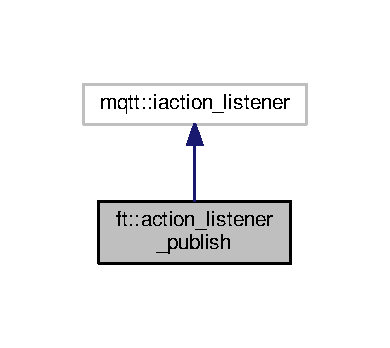
\includegraphics[width=187pt]{classft_1_1action__listener__publish__inherit__graph}
\end{center}
\end{figure}


Collaboration diagram for ft\+:\+:action\+\_\+listener\+\_\+publish\+:
\nopagebreak
\begin{figure}[H]
\begin{center}
\leavevmode
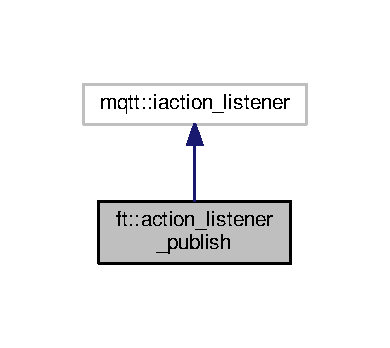
\includegraphics[width=187pt]{classft_1_1action__listener__publish__coll__graph}
\end{center}
\end{figure}
\subsection*{Public Member Functions}
\begin{DoxyCompactItemize}
\item 
\hyperlink{classft_1_1action__listener__publish_a057309964d2f4bbb5f10c31b8e6b6a31}{action\+\_\+listener\+\_\+publish} ()
\end{DoxyCompactItemize}


\subsection{Constructor \& Destructor Documentation}
\index{ft\+::action\+\_\+listener\+\_\+publish@{ft\+::action\+\_\+listener\+\_\+publish}!action\+\_\+listener\+\_\+publish@{action\+\_\+listener\+\_\+publish}}
\index{action\+\_\+listener\+\_\+publish@{action\+\_\+listener\+\_\+publish}!ft\+::action\+\_\+listener\+\_\+publish@{ft\+::action\+\_\+listener\+\_\+publish}}
\subsubsection[{\texorpdfstring{action\+\_\+listener\+\_\+publish()}{action_listener_publish()}}]{\setlength{\rightskip}{0pt plus 5cm}ft\+::action\+\_\+listener\+\_\+publish\+::action\+\_\+listener\+\_\+publish (
\begin{DoxyParamCaption}
{}
\end{DoxyParamCaption}
)\hspace{0.3cm}{\ttfamily [inline]}}\hypertarget{classft_1_1action__listener__publish_a057309964d2f4bbb5f10c31b8e6b6a31}{}\label{classft_1_1action__listener__publish_a057309964d2f4bbb5f10c31b8e6b6a31}


The documentation for this class was generated from the following file\+:\begin{DoxyCompactItemize}
\item 
\hyperlink{_txt_mqtt_factory_client_8h}{Txt\+Mqtt\+Factory\+Client.\+h}\end{DoxyCompactItemize}

\hypertarget{classft_1_1action__listener__subscribe}{}\section{ft\+:\+:action\+\_\+listener\+\_\+subscribe Class Reference}
\label{classft_1_1action__listener__subscribe}\index{ft\+::action\+\_\+listener\+\_\+subscribe@{ft\+::action\+\_\+listener\+\_\+subscribe}}


{\ttfamily \#include $<$Txt\+Mqtt\+Factory\+Client.\+h$>$}



Inheritance diagram for ft\+:\+:action\+\_\+listener\+\_\+subscribe\+:
\nopagebreak
\begin{figure}[H]
\begin{center}
\leavevmode
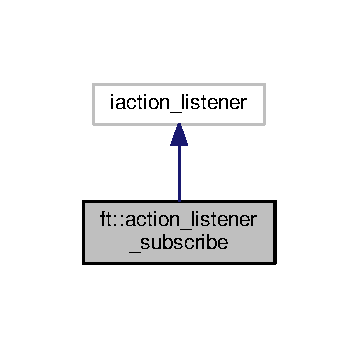
\includegraphics[width=172pt]{classft_1_1action__listener__subscribe__inherit__graph}
\end{center}
\end{figure}


Collaboration diagram for ft\+:\+:action\+\_\+listener\+\_\+subscribe\+:
\nopagebreak
\begin{figure}[H]
\begin{center}
\leavevmode
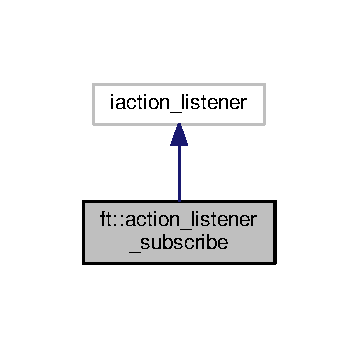
\includegraphics[width=172pt]{classft_1_1action__listener__subscribe__coll__graph}
\end{center}
\end{figure}
\subsection*{Public Member Functions}
\begin{DoxyCompactItemize}
\item 
\hyperlink{classft_1_1action__listener__subscribe_a478c36f7f546df16a22a35dd380224e8}{action\+\_\+listener\+\_\+subscribe} ()
\end{DoxyCompactItemize}


\subsection{Constructor \& Destructor Documentation}
\index{ft\+::action\+\_\+listener\+\_\+subscribe@{ft\+::action\+\_\+listener\+\_\+subscribe}!action\+\_\+listener\+\_\+subscribe@{action\+\_\+listener\+\_\+subscribe}}
\index{action\+\_\+listener\+\_\+subscribe@{action\+\_\+listener\+\_\+subscribe}!ft\+::action\+\_\+listener\+\_\+subscribe@{ft\+::action\+\_\+listener\+\_\+subscribe}}
\subsubsection[{\texorpdfstring{action\+\_\+listener\+\_\+subscribe()}{action_listener_subscribe()}}]{\setlength{\rightskip}{0pt plus 5cm}ft\+::action\+\_\+listener\+\_\+subscribe\+::action\+\_\+listener\+\_\+subscribe (
\begin{DoxyParamCaption}
{}
\end{DoxyParamCaption}
)\hspace{0.3cm}{\ttfamily [inline]}}\hypertarget{classft_1_1action__listener__subscribe_a478c36f7f546df16a22a35dd380224e8}{}\label{classft_1_1action__listener__subscribe_a478c36f7f546df16a22a35dd380224e8}


The documentation for this class was generated from the following file\+:\begin{DoxyCompactItemize}
\item 
\hyperlink{_txt_mqtt_factory_client_8h}{Txt\+Mqtt\+Factory\+Client.\+h}\end{DoxyCompactItemize}

\hypertarget{structft_1_1_bitset}{}\section{ft\+:\+:Bitset$<$ T $>$ Struct Template Reference}
\label{structft_1_1_bitset}\index{ft\+::\+Bitset$<$ T $>$@{ft\+::\+Bitset$<$ T $>$}}


{\ttfamily \#include $<$Txt\+Alert.\+h$>$}

\subsection*{Public Member Functions}
\begin{DoxyCompactItemize}
\item 
\hyperlink{structft_1_1_bitset_a6036ac7a0f723a3b7bbfc755d789f3e7}{Bitset} (T value)
\item 
void \hyperlink{structft_1_1_bitset_a51c87cd661e7965248afa96afe519601}{Modify} (int index, bool bit)
\item 
bool \hyperlink{structft_1_1_bitset_a278b8718fb98de6f2b137648356c2399}{Get} (int index) const 
\item 
T \hyperlink{structft_1_1_bitset_a6de68cecb43573b8f976f5220206c102}{Get\+Value} () const 
\end{DoxyCompactItemize}


\subsection{Constructor \& Destructor Documentation}
\index{ft\+::\+Bitset@{ft\+::\+Bitset}!Bitset@{Bitset}}
\index{Bitset@{Bitset}!ft\+::\+Bitset@{ft\+::\+Bitset}}
\subsubsection[{\texorpdfstring{Bitset(\+T value)}{Bitset(T value)}}]{\setlength{\rightskip}{0pt plus 5cm}template$<$typename T$>$ {\bf ft\+::\+Bitset}$<$ T $>$\+::{\bf Bitset} (
\begin{DoxyParamCaption}
\item[{T}]{value}
\end{DoxyParamCaption}
)\hspace{0.3cm}{\ttfamily [inline]}}\hypertarget{structft_1_1_bitset_a6036ac7a0f723a3b7bbfc755d789f3e7}{}\label{structft_1_1_bitset_a6036ac7a0f723a3b7bbfc755d789f3e7}


\subsection{Member Function Documentation}
\index{ft\+::\+Bitset@{ft\+::\+Bitset}!Get@{Get}}
\index{Get@{Get}!ft\+::\+Bitset@{ft\+::\+Bitset}}
\subsubsection[{\texorpdfstring{Get(int index) const }{Get(int index) const }}]{\setlength{\rightskip}{0pt plus 5cm}template$<$typename T$>$ bool {\bf ft\+::\+Bitset}$<$ T $>$\+::Get (
\begin{DoxyParamCaption}
\item[{int}]{index}
\end{DoxyParamCaption}
) const\hspace{0.3cm}{\ttfamily [inline]}}\hypertarget{structft_1_1_bitset_a278b8718fb98de6f2b137648356c2399}{}\label{structft_1_1_bitset_a278b8718fb98de6f2b137648356c2399}
\index{ft\+::\+Bitset@{ft\+::\+Bitset}!Get\+Value@{Get\+Value}}
\index{Get\+Value@{Get\+Value}!ft\+::\+Bitset@{ft\+::\+Bitset}}
\subsubsection[{\texorpdfstring{Get\+Value() const }{GetValue() const }}]{\setlength{\rightskip}{0pt plus 5cm}template$<$typename T$>$ T {\bf ft\+::\+Bitset}$<$ T $>$\+::Get\+Value (
\begin{DoxyParamCaption}
{}
\end{DoxyParamCaption}
) const\hspace{0.3cm}{\ttfamily [inline]}}\hypertarget{structft_1_1_bitset_a6de68cecb43573b8f976f5220206c102}{}\label{structft_1_1_bitset_a6de68cecb43573b8f976f5220206c102}
\index{ft\+::\+Bitset@{ft\+::\+Bitset}!Modify@{Modify}}
\index{Modify@{Modify}!ft\+::\+Bitset@{ft\+::\+Bitset}}
\subsubsection[{\texorpdfstring{Modify(int index, bool bit)}{Modify(int index, bool bit)}}]{\setlength{\rightskip}{0pt plus 5cm}template$<$typename T$>$ void {\bf ft\+::\+Bitset}$<$ T $>$\+::Modify (
\begin{DoxyParamCaption}
\item[{int}]{index, }
\item[{bool}]{bit}
\end{DoxyParamCaption}
)\hspace{0.3cm}{\ttfamily [inline]}}\hypertarget{structft_1_1_bitset_a51c87cd661e7965248afa96afe519601}{}\label{structft_1_1_bitset_a51c87cd661e7965248afa96afe519601}


The documentation for this struct was generated from the following file\+:\begin{DoxyCompactItemize}
\item 
\hyperlink{_txt_alert_8h}{Txt\+Alert.\+h}\end{DoxyCompactItemize}

\hypertarget{classft_1_1_enc_pos2}{}\section{ft\+:\+:Enc\+Pos2 Class Reference}
\label{classft_1_1_enc_pos2}\index{ft\+::\+Enc\+Pos2@{ft\+::\+Enc\+Pos2}}


{\ttfamily \#include $<$Txt\+Factory\+Types.\+h$>$}

\subsection*{Public Member Functions}
\begin{DoxyCompactItemize}
\item 
\hyperlink{classft_1_1_enc_pos2_adbf5070464ebea517ad87bca1d8b5be4}{Enc\+Pos2} (uint16\+\_\+t \hyperlink{classft_1_1_enc_pos2_a072f8a1be35ff117c08f4b82b3eb3b38}{x}=0, uint16\+\_\+t \hyperlink{classft_1_1_enc_pos2_ae71ca727428ff924d60efc2281e196dc}{y}=0)
\end{DoxyCompactItemize}
\subsection*{Public Attributes}
\begin{DoxyCompactItemize}
\item 
uint16\+\_\+t \hyperlink{classft_1_1_enc_pos2_a072f8a1be35ff117c08f4b82b3eb3b38}{x}
\item 
uint16\+\_\+t \hyperlink{classft_1_1_enc_pos2_ae71ca727428ff924d60efc2281e196dc}{y}
\end{DoxyCompactItemize}


\subsection{Constructor \& Destructor Documentation}
\index{ft\+::\+Enc\+Pos2@{ft\+::\+Enc\+Pos2}!Enc\+Pos2@{Enc\+Pos2}}
\index{Enc\+Pos2@{Enc\+Pos2}!ft\+::\+Enc\+Pos2@{ft\+::\+Enc\+Pos2}}
\subsubsection[{\texorpdfstring{Enc\+Pos2(uint16\+\_\+t x=0, uint16\+\_\+t y=0)}{EncPos2(uint16_t x=0, uint16_t y=0)}}]{\setlength{\rightskip}{0pt plus 5cm}ft\+::\+Enc\+Pos2\+::\+Enc\+Pos2 (
\begin{DoxyParamCaption}
\item[{uint16\+\_\+t}]{x = {\ttfamily 0}, }
\item[{uint16\+\_\+t}]{y = {\ttfamily 0}}
\end{DoxyParamCaption}
)\hspace{0.3cm}{\ttfamily [inline]}}\hypertarget{classft_1_1_enc_pos2_adbf5070464ebea517ad87bca1d8b5be4}{}\label{classft_1_1_enc_pos2_adbf5070464ebea517ad87bca1d8b5be4}


\subsection{Member Data Documentation}
\index{ft\+::\+Enc\+Pos2@{ft\+::\+Enc\+Pos2}!x@{x}}
\index{x@{x}!ft\+::\+Enc\+Pos2@{ft\+::\+Enc\+Pos2}}
\subsubsection[{\texorpdfstring{x}{x}}]{\setlength{\rightskip}{0pt plus 5cm}uint16\+\_\+t ft\+::\+Enc\+Pos2\+::x}\hypertarget{classft_1_1_enc_pos2_a072f8a1be35ff117c08f4b82b3eb3b38}{}\label{classft_1_1_enc_pos2_a072f8a1be35ff117c08f4b82b3eb3b38}
\index{ft\+::\+Enc\+Pos2@{ft\+::\+Enc\+Pos2}!y@{y}}
\index{y@{y}!ft\+::\+Enc\+Pos2@{ft\+::\+Enc\+Pos2}}
\subsubsection[{\texorpdfstring{y}{y}}]{\setlength{\rightskip}{0pt plus 5cm}uint16\+\_\+t ft\+::\+Enc\+Pos2\+::y}\hypertarget{classft_1_1_enc_pos2_ae71ca727428ff924d60efc2281e196dc}{}\label{classft_1_1_enc_pos2_ae71ca727428ff924d60efc2281e196dc}


The documentation for this class was generated from the following file\+:\begin{DoxyCompactItemize}
\item 
\hyperlink{_txt_factory_types_8h}{Txt\+Factory\+Types.\+h}\end{DoxyCompactItemize}

\hypertarget{classft_1_1_enc_pos3}{}\section{ft\+:\+:Enc\+Pos3 Class Reference}
\label{classft_1_1_enc_pos3}\index{ft\+::\+Enc\+Pos3@{ft\+::\+Enc\+Pos3}}


{\ttfamily \#include $<$Txt\+Factory\+Types.\+h$>$}

\subsection*{Public Member Functions}
\begin{DoxyCompactItemize}
\item 
\hyperlink{classft_1_1_enc_pos3_aa9ff1058e2e06e2ae97aa99254006391}{Enc\+Pos3} (uint16\+\_\+t \hyperlink{classft_1_1_enc_pos3_ad03b62372f78ef0a141f4389f8e6c67d}{x}=0, uint16\+\_\+t \hyperlink{classft_1_1_enc_pos3_a2ed97861702c89ee83bef490c701e2c6}{y}=0, uint16\+\_\+t \hyperlink{classft_1_1_enc_pos3_a621ba71369e3cc2fb3461a944ec7d7e1}{z}=0)
\end{DoxyCompactItemize}
\subsection*{Public Attributes}
\begin{DoxyCompactItemize}
\item 
uint16\+\_\+t \hyperlink{classft_1_1_enc_pos3_ad03b62372f78ef0a141f4389f8e6c67d}{x}
\item 
uint16\+\_\+t \hyperlink{classft_1_1_enc_pos3_a2ed97861702c89ee83bef490c701e2c6}{y}
\item 
uint16\+\_\+t \hyperlink{classft_1_1_enc_pos3_a621ba71369e3cc2fb3461a944ec7d7e1}{z}
\end{DoxyCompactItemize}


\subsection{Constructor \& Destructor Documentation}
\index{ft\+::\+Enc\+Pos3@{ft\+::\+Enc\+Pos3}!Enc\+Pos3@{Enc\+Pos3}}
\index{Enc\+Pos3@{Enc\+Pos3}!ft\+::\+Enc\+Pos3@{ft\+::\+Enc\+Pos3}}
\subsubsection[{\texorpdfstring{Enc\+Pos3(uint16\+\_\+t x=0, uint16\+\_\+t y=0, uint16\+\_\+t z=0)}{EncPos3(uint16_t x=0, uint16_t y=0, uint16_t z=0)}}]{\setlength{\rightskip}{0pt plus 5cm}ft\+::\+Enc\+Pos3\+::\+Enc\+Pos3 (
\begin{DoxyParamCaption}
\item[{uint16\+\_\+t}]{x = {\ttfamily 0}, }
\item[{uint16\+\_\+t}]{y = {\ttfamily 0}, }
\item[{uint16\+\_\+t}]{z = {\ttfamily 0}}
\end{DoxyParamCaption}
)\hspace{0.3cm}{\ttfamily [inline]}}\hypertarget{classft_1_1_enc_pos3_aa9ff1058e2e06e2ae97aa99254006391}{}\label{classft_1_1_enc_pos3_aa9ff1058e2e06e2ae97aa99254006391}


\subsection{Member Data Documentation}
\index{ft\+::\+Enc\+Pos3@{ft\+::\+Enc\+Pos3}!x@{x}}
\index{x@{x}!ft\+::\+Enc\+Pos3@{ft\+::\+Enc\+Pos3}}
\subsubsection[{\texorpdfstring{x}{x}}]{\setlength{\rightskip}{0pt plus 5cm}uint16\+\_\+t ft\+::\+Enc\+Pos3\+::x}\hypertarget{classft_1_1_enc_pos3_ad03b62372f78ef0a141f4389f8e6c67d}{}\label{classft_1_1_enc_pos3_ad03b62372f78ef0a141f4389f8e6c67d}
\index{ft\+::\+Enc\+Pos3@{ft\+::\+Enc\+Pos3}!y@{y}}
\index{y@{y}!ft\+::\+Enc\+Pos3@{ft\+::\+Enc\+Pos3}}
\subsubsection[{\texorpdfstring{y}{y}}]{\setlength{\rightskip}{0pt plus 5cm}uint16\+\_\+t ft\+::\+Enc\+Pos3\+::y}\hypertarget{classft_1_1_enc_pos3_a2ed97861702c89ee83bef490c701e2c6}{}\label{classft_1_1_enc_pos3_a2ed97861702c89ee83bef490c701e2c6}
\index{ft\+::\+Enc\+Pos3@{ft\+::\+Enc\+Pos3}!z@{z}}
\index{z@{z}!ft\+::\+Enc\+Pos3@{ft\+::\+Enc\+Pos3}}
\subsubsection[{\texorpdfstring{z}{z}}]{\setlength{\rightskip}{0pt plus 5cm}uint16\+\_\+t ft\+::\+Enc\+Pos3\+::z}\hypertarget{classft_1_1_enc_pos3_a621ba71369e3cc2fb3461a944ec7d7e1}{}\label{classft_1_1_enc_pos3_a621ba71369e3cc2fb3461a944ec7d7e1}


The documentation for this class was generated from the following file\+:\begin{DoxyCompactItemize}
\item 
\hyperlink{_txt_factory_types_8h}{Txt\+Factory\+Types.\+h}\end{DoxyCompactItemize}

\hypertarget{classft_1_1_observer}{}\section{ft\+:\+:Observer Class Reference}
\label{classft_1_1_observer}\index{ft\+::\+Observer@{ft\+::\+Observer}}


{\ttfamily \#include $<$Observer.\+h$>$}



Inheritance diagram for ft\+:\+:Observer\+:
\nopagebreak
\begin{figure}[H]
\begin{center}
\leavevmode
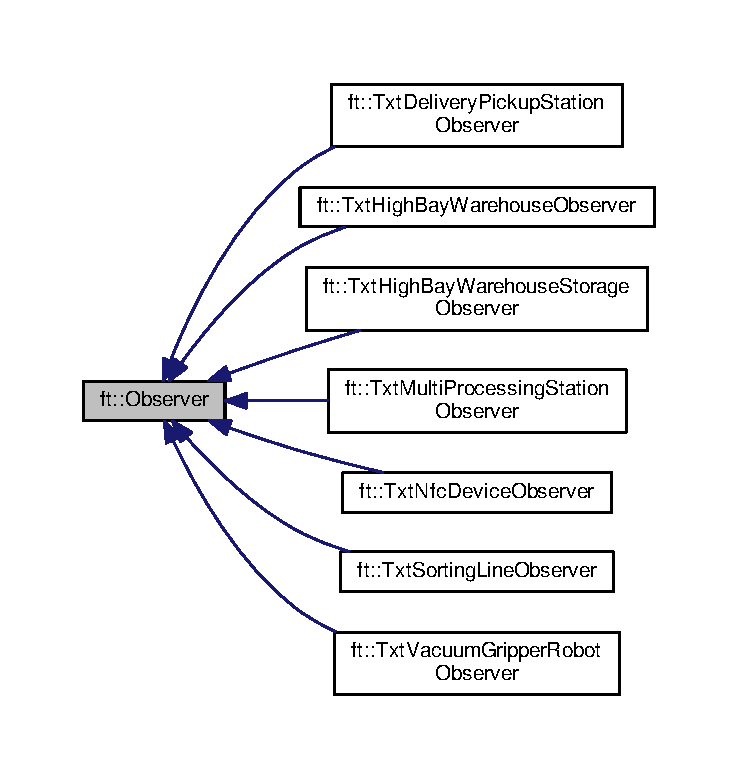
\includegraphics[width=350pt]{classft_1_1_observer__inherit__graph}
\end{center}
\end{figure}
\subsection*{Public Member Functions}
\begin{DoxyCompactItemize}
\item 
\hyperlink{classft_1_1_observer_a887b595b0a31f9486cacce9f797e666d}{Observer} ()
\item 
virtual \hyperlink{classft_1_1_observer_a1b4aedb717c95fa0dc2c4f5bca50a608}{$\sim$\+Observer} ()
\item 
virtual void \hyperlink{classft_1_1_observer_aeea41c77afbd09f595a4290954a5aa66}{Update} (\hyperlink{classft_1_1_subject_observer}{Subject\+Observer} $\ast$the\+Change\+Subject)=0
\end{DoxyCompactItemize}


\subsection{Constructor \& Destructor Documentation}
\index{ft\+::\+Observer@{ft\+::\+Observer}!Observer@{Observer}}
\index{Observer@{Observer}!ft\+::\+Observer@{ft\+::\+Observer}}
\subsubsection[{\texorpdfstring{Observer()}{Observer()}}]{\setlength{\rightskip}{0pt plus 5cm}ft\+::\+Observer\+::\+Observer (
\begin{DoxyParamCaption}
{}
\end{DoxyParamCaption}
)\hspace{0.3cm}{\ttfamily [inline]}}\hypertarget{classft_1_1_observer_a887b595b0a31f9486cacce9f797e666d}{}\label{classft_1_1_observer_a887b595b0a31f9486cacce9f797e666d}
\index{ft\+::\+Observer@{ft\+::\+Observer}!````~Observer@{$\sim$\+Observer}}
\index{````~Observer@{$\sim$\+Observer}!ft\+::\+Observer@{ft\+::\+Observer}}
\subsubsection[{\texorpdfstring{$\sim$\+Observer()}{~Observer()}}]{\setlength{\rightskip}{0pt plus 5cm}virtual ft\+::\+Observer\+::$\sim$\+Observer (
\begin{DoxyParamCaption}
{}
\end{DoxyParamCaption}
)\hspace{0.3cm}{\ttfamily [inline]}, {\ttfamily [virtual]}}\hypertarget{classft_1_1_observer_a1b4aedb717c95fa0dc2c4f5bca50a608}{}\label{classft_1_1_observer_a1b4aedb717c95fa0dc2c4f5bca50a608}


\subsection{Member Function Documentation}
\index{ft\+::\+Observer@{ft\+::\+Observer}!Update@{Update}}
\index{Update@{Update}!ft\+::\+Observer@{ft\+::\+Observer}}
\subsubsection[{\texorpdfstring{Update(\+Subject\+Observer $\ast$the\+Change\+Subject)=0}{Update(SubjectObserver *theChangeSubject)=0}}]{\setlength{\rightskip}{0pt plus 5cm}virtual void ft\+::\+Observer\+::\+Update (
\begin{DoxyParamCaption}
\item[{{\bf Subject\+Observer} $\ast$}]{the\+Change\+Subject}
\end{DoxyParamCaption}
)\hspace{0.3cm}{\ttfamily [pure virtual]}}\hypertarget{classft_1_1_observer_aeea41c77afbd09f595a4290954a5aa66}{}\label{classft_1_1_observer_aeea41c77afbd09f595a4290954a5aa66}


Implemented in \hyperlink{classft_1_1_txt_vacuum_gripper_robot_observer_a7359c1fad15ca0f0354700b3cb86e13f}{ft\+::\+Txt\+Vacuum\+Gripper\+Robot\+Observer}, \hyperlink{classft_1_1_txt_high_bay_warehouse_observer_ac3519a699f526f34d39bf6be04f00ff6}{ft\+::\+Txt\+High\+Bay\+Warehouse\+Observer}, \hyperlink{classft_1_1_txt_sorting_line_observer_a4948d5d5c3981866bdc2efe747c06000}{ft\+::\+Txt\+Sorting\+Line\+Observer}, \hyperlink{classft_1_1_txt_multi_processing_station_observer_aeddc4246174e6fd5aaa75823416c5e85}{ft\+::\+Txt\+Multi\+Processing\+Station\+Observer}, \hyperlink{classft_1_1_txt_delivery_pickup_station_observer_a2525d061949c0b3c282b485c7ee0592b}{ft\+::\+Txt\+Delivery\+Pickup\+Station\+Observer}, \hyperlink{classft_1_1_txt_nfc_device_observer_a32311fe745e0777842453ef8b93083b8}{ft\+::\+Txt\+Nfc\+Device\+Observer}, and \hyperlink{classft_1_1_txt_high_bay_warehouse_storage_observer_a0ed13d06ea759d8840fbd1932b203b40}{ft\+::\+Txt\+High\+Bay\+Warehouse\+Storage\+Observer}.



The documentation for this class was generated from the following file\+:\begin{DoxyCompactItemize}
\item 
\hyperlink{_observer_8h}{Observer.\+h}\end{DoxyCompactItemize}

\hypertarget{structft_1_1_storage_pos2}{}\section{ft\+:\+:Storage\+Pos2 Struct Reference}
\label{structft_1_1_storage_pos2}\index{ft\+::\+Storage\+Pos2@{ft\+::\+Storage\+Pos2}}


{\ttfamily \#include $<$Txt\+High\+Bay\+Warehouse\+Storage.\+h$>$}

\subsection*{Public Attributes}
\begin{DoxyCompactItemize}
\item 
int \hyperlink{structft_1_1_storage_pos2_ac08eedb92bdec6ec5271afc19e4102b9}{x}
\item 
int \hyperlink{structft_1_1_storage_pos2_a7b7946c712f12343cbe903623b06f704}{y}
\end{DoxyCompactItemize}


\subsection{Member Data Documentation}
\index{ft\+::\+Storage\+Pos2@{ft\+::\+Storage\+Pos2}!x@{x}}
\index{x@{x}!ft\+::\+Storage\+Pos2@{ft\+::\+Storage\+Pos2}}
\subsubsection[{\texorpdfstring{x}{x}}]{\setlength{\rightskip}{0pt plus 5cm}int ft\+::\+Storage\+Pos2\+::x}\hypertarget{structft_1_1_storage_pos2_ac08eedb92bdec6ec5271afc19e4102b9}{}\label{structft_1_1_storage_pos2_ac08eedb92bdec6ec5271afc19e4102b9}
\index{ft\+::\+Storage\+Pos2@{ft\+::\+Storage\+Pos2}!y@{y}}
\index{y@{y}!ft\+::\+Storage\+Pos2@{ft\+::\+Storage\+Pos2}}
\subsubsection[{\texorpdfstring{y}{y}}]{\setlength{\rightskip}{0pt plus 5cm}int ft\+::\+Storage\+Pos2\+::y}\hypertarget{structft_1_1_storage_pos2_a7b7946c712f12343cbe903623b06f704}{}\label{structft_1_1_storage_pos2_a7b7946c712f12343cbe903623b06f704}


The documentation for this struct was generated from the following file\+:\begin{DoxyCompactItemize}
\item 
\hyperlink{_txt_high_bay_warehouse_storage_8h}{Txt\+High\+Bay\+Warehouse\+Storage.\+h}\end{DoxyCompactItemize}

\hypertarget{classft_1_1_subject_observer}{}\section{ft\+:\+:Subject\+Observer Class Reference}
\label{classft_1_1_subject_observer}\index{ft\+::\+Subject\+Observer@{ft\+::\+Subject\+Observer}}


{\ttfamily \#include $<$Observer.\+h$>$}



Inheritance diagram for ft\+:\+:Subject\+Observer\+:
\nopagebreak
\begin{figure}[H]
\begin{center}
\leavevmode
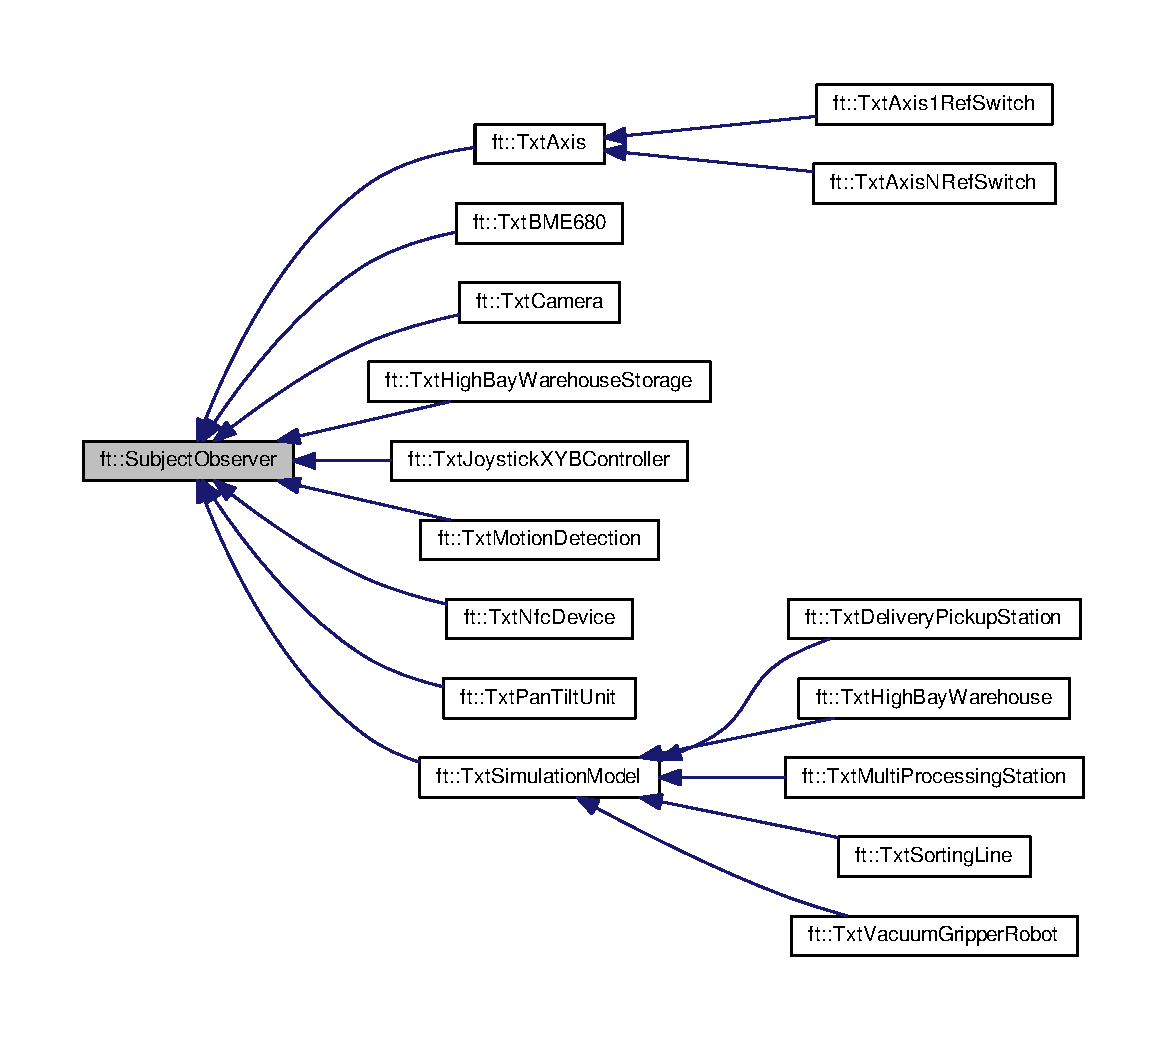
\includegraphics[width=350pt]{classft_1_1_subject_observer__inherit__graph}
\end{center}
\end{figure}
\subsection*{Public Member Functions}
\begin{DoxyCompactItemize}
\item 
\hyperlink{classft_1_1_subject_observer_aac5d28f22abe6a477d5dc3ea3be2b89e}{Subject\+Observer} ()
\item 
virtual \hyperlink{classft_1_1_subject_observer_a19735bd75211a7f2fbd3401e50184667}{$\sim$\+Subject\+Observer} ()
\item 
virtual void \hyperlink{classft_1_1_subject_observer_a94332adb13ba0f1e610287dfbeccc18d}{Attach} (\hyperlink{classft_1_1_observer}{Observer} $\ast$)
\item 
virtual void \hyperlink{classft_1_1_subject_observer_acf9ba0790274c926591f11be33e36ac6}{Detach} (\hyperlink{classft_1_1_observer}{Observer} $\ast$)
\item 
virtual void \hyperlink{classft_1_1_subject_observer_a5a797eb3e2c13bbd3bdf122894bd29e9}{Notify} ()
\end{DoxyCompactItemize}


\subsection{Constructor \& Destructor Documentation}
\index{ft\+::\+Subject\+Observer@{ft\+::\+Subject\+Observer}!Subject\+Observer@{Subject\+Observer}}
\index{Subject\+Observer@{Subject\+Observer}!ft\+::\+Subject\+Observer@{ft\+::\+Subject\+Observer}}
\subsubsection[{\texorpdfstring{Subject\+Observer()}{SubjectObserver()}}]{\setlength{\rightskip}{0pt plus 5cm}ft\+::\+Subject\+Observer\+::\+Subject\+Observer (
\begin{DoxyParamCaption}
{}
\end{DoxyParamCaption}
)\hspace{0.3cm}{\ttfamily [inline]}}\hypertarget{classft_1_1_subject_observer_aac5d28f22abe6a477d5dc3ea3be2b89e}{}\label{classft_1_1_subject_observer_aac5d28f22abe6a477d5dc3ea3be2b89e}
\index{ft\+::\+Subject\+Observer@{ft\+::\+Subject\+Observer}!````~Subject\+Observer@{$\sim$\+Subject\+Observer}}
\index{````~Subject\+Observer@{$\sim$\+Subject\+Observer}!ft\+::\+Subject\+Observer@{ft\+::\+Subject\+Observer}}
\subsubsection[{\texorpdfstring{$\sim$\+Subject\+Observer()}{~SubjectObserver()}}]{\setlength{\rightskip}{0pt plus 5cm}virtual ft\+::\+Subject\+Observer\+::$\sim$\+Subject\+Observer (
\begin{DoxyParamCaption}
{}
\end{DoxyParamCaption}
)\hspace{0.3cm}{\ttfamily [inline]}, {\ttfamily [virtual]}}\hypertarget{classft_1_1_subject_observer_a19735bd75211a7f2fbd3401e50184667}{}\label{classft_1_1_subject_observer_a19735bd75211a7f2fbd3401e50184667}


\subsection{Member Function Documentation}
\index{ft\+::\+Subject\+Observer@{ft\+::\+Subject\+Observer}!Attach@{Attach}}
\index{Attach@{Attach}!ft\+::\+Subject\+Observer@{ft\+::\+Subject\+Observer}}
\subsubsection[{\texorpdfstring{Attach(\+Observer $\ast$)}{Attach(Observer *)}}]{\setlength{\rightskip}{0pt plus 5cm}virtual void ft\+::\+Subject\+Observer\+::\+Attach (
\begin{DoxyParamCaption}
\item[{{\bf Observer} $\ast$}]{}
\end{DoxyParamCaption}
)\hspace{0.3cm}{\ttfamily [virtual]}}\hypertarget{classft_1_1_subject_observer_a94332adb13ba0f1e610287dfbeccc18d}{}\label{classft_1_1_subject_observer_a94332adb13ba0f1e610287dfbeccc18d}
\index{ft\+::\+Subject\+Observer@{ft\+::\+Subject\+Observer}!Detach@{Detach}}
\index{Detach@{Detach}!ft\+::\+Subject\+Observer@{ft\+::\+Subject\+Observer}}
\subsubsection[{\texorpdfstring{Detach(\+Observer $\ast$)}{Detach(Observer *)}}]{\setlength{\rightskip}{0pt plus 5cm}virtual void ft\+::\+Subject\+Observer\+::\+Detach (
\begin{DoxyParamCaption}
\item[{{\bf Observer} $\ast$}]{}
\end{DoxyParamCaption}
)\hspace{0.3cm}{\ttfamily [virtual]}}\hypertarget{classft_1_1_subject_observer_acf9ba0790274c926591f11be33e36ac6}{}\label{classft_1_1_subject_observer_acf9ba0790274c926591f11be33e36ac6}
\index{ft\+::\+Subject\+Observer@{ft\+::\+Subject\+Observer}!Notify@{Notify}}
\index{Notify@{Notify}!ft\+::\+Subject\+Observer@{ft\+::\+Subject\+Observer}}
\subsubsection[{\texorpdfstring{Notify()}{Notify()}}]{\setlength{\rightskip}{0pt plus 5cm}virtual void ft\+::\+Subject\+Observer\+::\+Notify (
\begin{DoxyParamCaption}
{}
\end{DoxyParamCaption}
)\hspace{0.3cm}{\ttfamily [virtual]}}\hypertarget{classft_1_1_subject_observer_a5a797eb3e2c13bbd3bdf122894bd29e9}{}\label{classft_1_1_subject_observer_a5a797eb3e2c13bbd3bdf122894bd29e9}


The documentation for this class was generated from the following file\+:\begin{DoxyCompactItemize}
\item 
\hyperlink{_observer_8h}{Observer.\+h}\end{DoxyCompactItemize}

\hypertarget{unionft_1_1ts__u}{}\section{ft\+:\+:ts\+\_\+u Union Reference}
\label{unionft_1_1ts__u}\index{ft\+::ts\+\_\+u@{ft\+::ts\+\_\+u}}


{\ttfamily \#include $<$Txt\+Nfc\+Device.\+h$>$}

\subsection*{Public Attributes}
\begin{DoxyCompactItemize}
\item 
uint8\+\_\+t \hyperlink{unionft_1_1ts__u_a2bd6e7eefdc25ffe6105540f7cbb8022}{u8} \mbox{[}8\mbox{]}
\item 
int64\+\_\+t \hyperlink{unionft_1_1ts__u_a3f0ddb56ec7ef6f9ee1d75e89a968a9a}{s64}
\end{DoxyCompactItemize}


\subsection{Member Data Documentation}
\index{ft\+::ts\+\_\+u@{ft\+::ts\+\_\+u}!s64@{s64}}
\index{s64@{s64}!ft\+::ts\+\_\+u@{ft\+::ts\+\_\+u}}
\subsubsection[{\texorpdfstring{s64}{s64}}]{\setlength{\rightskip}{0pt plus 5cm}int64\+\_\+t ft\+::ts\+\_\+u\+::s64}\hypertarget{unionft_1_1ts__u_a3f0ddb56ec7ef6f9ee1d75e89a968a9a}{}\label{unionft_1_1ts__u_a3f0ddb56ec7ef6f9ee1d75e89a968a9a}
\index{ft\+::ts\+\_\+u@{ft\+::ts\+\_\+u}!u8@{u8}}
\index{u8@{u8}!ft\+::ts\+\_\+u@{ft\+::ts\+\_\+u}}
\subsubsection[{\texorpdfstring{u8}{u8}}]{\setlength{\rightskip}{0pt plus 5cm}uint8\+\_\+t ft\+::ts\+\_\+u\+::u8\mbox{[}8\mbox{]}}\hypertarget{unionft_1_1ts__u_a2bd6e7eefdc25ffe6105540f7cbb8022}{}\label{unionft_1_1ts__u_a2bd6e7eefdc25ffe6105540f7cbb8022}


The documentation for this union was generated from the following file\+:\begin{DoxyCompactItemize}
\item 
\hyperlink{_txt_nfc_device_8h}{Txt\+Nfc\+Device.\+h}\end{DoxyCompactItemize}

\hypertarget{classft_1_1_txt_axis}{}\section{ft\+:\+:Txt\+Axis Class Reference}
\label{classft_1_1_txt_axis}\index{ft\+::\+Txt\+Axis@{ft\+::\+Txt\+Axis}}


{\ttfamily \#include $<$Txt\+Axis.\+h$>$}



Inheritance diagram for ft\+:\+:Txt\+Axis\+:
\nopagebreak
\begin{figure}[H]
\begin{center}
\leavevmode
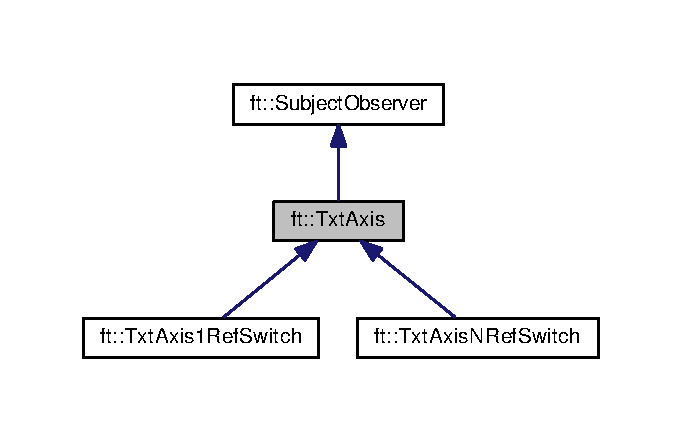
\includegraphics[width=328pt]{classft_1_1_txt_axis__inherit__graph}
\end{center}
\end{figure}


Collaboration diagram for ft\+:\+:Txt\+Axis\+:
\nopagebreak
\begin{figure}[H]
\begin{center}
\leavevmode
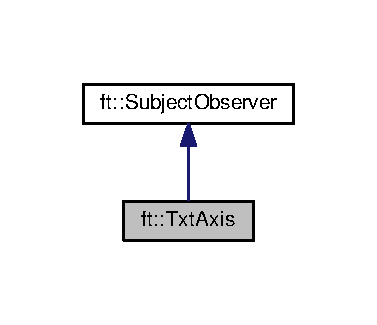
\includegraphics[width=181pt]{classft_1_1_txt_axis__coll__graph}
\end{center}
\end{figure}
\subsection*{Public Member Functions}
\begin{DoxyCompactItemize}
\item 
\hyperlink{classft_1_1_txt_axis_ab381c0ebcd4cae9df6d98287bacfd07f}{Txt\+Axis} (std\+::string \hyperlink{classft_1_1_txt_axis_a358af2b2ed1709b40ab6c9768c2795ef}{name}, F\+I\+S\+H\+\_\+\+X1\+\_\+\+T\+R\+A\+N\+S\+F\+ER $\ast$\hyperlink{classft_1_1_txt_axis_ae5521c2eda7b80599ed6340f6a8192f2}{p\+T\+Area}, uint8\+\_\+t \hyperlink{classft_1_1_txt_axis_a3a8988acb2f578fe96312221205c50c4}{chM}, uint8\+\_\+t \hyperlink{classft_1_1_txt_axis_a9b155580a8dcc876c8e0c4b9c92041e7}{ch\+S1})
\item 
virtual \hyperlink{classft_1_1_txt_axis_a7870184dba5c3e52edab4b69aa21d0cf}{$\sim$\+Txt\+Axis} ()
\item 
bool \hyperlink{classft_1_1_txt_axis_abec2d76398791fe4580fb38e0a25abe3}{init} ()
\item 
\hyperlink{namespaceft_a05630ec9d5a49c43a00ca107cfe6b350}{Txt\+Axis\+\_\+status\+\_\+t} \hyperlink{classft_1_1_txt_axis_acc8c2c6a1364a46c3147ea4d6b37a97c}{get\+Status} ()
\item 
void \hyperlink{classft_1_1_txt_axis_ad35a7e103aa3054302dd89c892c754b4}{set\+Speed} (int16\+\_\+t s)
\item 
int16\+\_\+t \hyperlink{classft_1_1_txt_axis_a83dd19fa863d5cf0d374f3bb0ab6c2af}{get\+Speed} ()
\item 
uint16\+\_\+t \hyperlink{classft_1_1_txt_axis_a1379066c1b28588283e2dc9f1e7aea11}{get\+Pos\+Abs} ()
\item 
void \hyperlink{classft_1_1_txt_axis_ab67bcbd24996bb94f9daedadd304e8d6}{stop} ()
\item 
virtual bool \hyperlink{classft_1_1_txt_axis_a0ae92e37ed640f5d65e59cd1ae6fe9cf}{move\+Abs} (uint16\+\_\+t p)
\item 
std\+::thread \hyperlink{classft_1_1_txt_axis_a319c02fb4ac1e1e3d86d8c126d5aee04}{move\+Abs\+Thread} (uint16\+\_\+t p)
\item 
bool \hyperlink{classft_1_1_txt_axis_a7b6f1cf66ca1e0668a5c689c0c8f6531}{move\+Rel} (int rp)
\item 
void \hyperlink{classft_1_1_txt_axis_ae8b0cb457a477a20ff932efeddbcd991}{move\+Ref} ()
\item 
std\+::thread \hyperlink{classft_1_1_txt_axis_a6a40c2cb6993b94a3c47aab8181545fa}{move\+Ref\+Thread} ()
\end{DoxyCompactItemize}
\subsection*{Protected Member Functions}
\begin{DoxyCompactItemize}
\item 
void \hyperlink{classft_1_1_txt_axis_a5c2e17eee902a907ee3ab108dd4faf02}{set\+Status} (\hyperlink{namespaceft_a05630ec9d5a49c43a00ca107cfe6b350}{Txt\+Axis\+\_\+status\+\_\+t} \hyperlink{classft_1_1_txt_axis_a2f74c132b00116f57ceb65cab7a525ee}{status})
\item 
void \hyperlink{classft_1_1_txt_axis_a1abdff278919fee8c859fdd080bf82ff}{reset} ()
\item 
void \hyperlink{classft_1_1_txt_axis_adf2ff312dd0eec4ec2e70c9979a93d7d}{reset\+Counter} ()
\item 
virtual void \hyperlink{classft_1_1_txt_axis_a39b5715dab5637e92f2ca817a05be930}{set\+Motor\+Off} ()
\item 
virtual void \hyperlink{classft_1_1_txt_axis_a408c5cfc000eb1f5ab49db8713906b27}{set\+Motor\+Left} ()
\item 
virtual void \hyperlink{classft_1_1_txt_axis_ae5398be07f55ebf29cd99969f846be30}{move\+Left} (uint16\+\_\+t steps, uint16\+\_\+t $\ast$p\+Pos)
\item 
virtual void \hyperlink{classft_1_1_txt_axis_aac0aaaa04969160f42542e76057ccb75}{move\+Right} (uint16\+\_\+t steps, uint16\+\_\+t $\ast$p\+Pos)=0
\end{DoxyCompactItemize}
\subsection*{Protected Attributes}
\begin{DoxyCompactItemize}
\item 
std\+::string \hyperlink{classft_1_1_txt_axis_a358af2b2ed1709b40ab6c9768c2795ef}{name}
\item 
F\+I\+S\+H\+\_\+\+X1\+\_\+\+T\+R\+A\+N\+S\+F\+ER $\ast$ \hyperlink{classft_1_1_txt_axis_ae5521c2eda7b80599ed6340f6a8192f2}{p\+T\+Area}
\item 
\hyperlink{namespaceft_a05630ec9d5a49c43a00ca107cfe6b350}{Txt\+Axis\+\_\+status\+\_\+t} \hyperlink{classft_1_1_txt_axis_a2f74c132b00116f57ceb65cab7a525ee}{status}
\item 
uint16\+\_\+t \hyperlink{classft_1_1_txt_axis_a51ccb254804e142bc26604e1efe94725}{pos}
\item 
int16\+\_\+t \hyperlink{classft_1_1_txt_axis_a3103b6972533eaac191a0a9e5c2e0564}{speed}
\item 
bool \hyperlink{classft_1_1_txt_axis_a27e59819797bfc1885d2fc4d3ebbe209}{stop\+Req}
\item 
uint8\+\_\+t \hyperlink{classft_1_1_txt_axis_a3a8988acb2f578fe96312221205c50c4}{chM}
\item 
uint8\+\_\+t \hyperlink{classft_1_1_txt_axis_a9b155580a8dcc876c8e0c4b9c92041e7}{ch\+S1}
\end{DoxyCompactItemize}
\subsection*{Friends}
\begin{DoxyCompactItemize}
\item 
class \hyperlink{classft_1_1_txt_axis_aea03938f89578033a66fa5dba1f9fe09}{Txt\+Vacuum\+Gripper\+Robot}
\item 
class \hyperlink{classft_1_1_txt_axis_ae0c44dc668d7ae80ecedb8484adf9fdf}{Txt\+High\+Bay\+Warehouse}
\end{DoxyCompactItemize}


\subsection{Constructor \& Destructor Documentation}
\index{ft\+::\+Txt\+Axis@{ft\+::\+Txt\+Axis}!Txt\+Axis@{Txt\+Axis}}
\index{Txt\+Axis@{Txt\+Axis}!ft\+::\+Txt\+Axis@{ft\+::\+Txt\+Axis}}
\subsubsection[{\texorpdfstring{Txt\+Axis(std\+::string name, F\+I\+S\+H\+\_\+\+X1\+\_\+\+T\+R\+A\+N\+S\+F\+E\+R $\ast$p\+T\+Area, uint8\+\_\+t ch\+M, uint8\+\_\+t ch\+S1)}{TxtAxis(std::string name, FISH_X1_TRANSFER *pTArea, uint8_t chM, uint8_t chS1)}}]{\setlength{\rightskip}{0pt plus 5cm}ft\+::\+Txt\+Axis\+::\+Txt\+Axis (
\begin{DoxyParamCaption}
\item[{std\+::string}]{name, }
\item[{F\+I\+S\+H\+\_\+\+X1\+\_\+\+T\+R\+A\+N\+S\+F\+ER $\ast$}]{p\+T\+Area, }
\item[{uint8\+\_\+t}]{chM, }
\item[{uint8\+\_\+t}]{ch\+S1}
\end{DoxyParamCaption}
)}\hypertarget{classft_1_1_txt_axis_ab381c0ebcd4cae9df6d98287bacfd07f}{}\label{classft_1_1_txt_axis_ab381c0ebcd4cae9df6d98287bacfd07f}
\index{ft\+::\+Txt\+Axis@{ft\+::\+Txt\+Axis}!````~Txt\+Axis@{$\sim$\+Txt\+Axis}}
\index{````~Txt\+Axis@{$\sim$\+Txt\+Axis}!ft\+::\+Txt\+Axis@{ft\+::\+Txt\+Axis}}
\subsubsection[{\texorpdfstring{$\sim$\+Txt\+Axis()}{~TxtAxis()}}]{\setlength{\rightskip}{0pt plus 5cm}virtual ft\+::\+Txt\+Axis\+::$\sim$\+Txt\+Axis (
\begin{DoxyParamCaption}
{}
\end{DoxyParamCaption}
)\hspace{0.3cm}{\ttfamily [virtual]}}\hypertarget{classft_1_1_txt_axis_a7870184dba5c3e52edab4b69aa21d0cf}{}\label{classft_1_1_txt_axis_a7870184dba5c3e52edab4b69aa21d0cf}


\subsection{Member Function Documentation}
\index{ft\+::\+Txt\+Axis@{ft\+::\+Txt\+Axis}!get\+Pos\+Abs@{get\+Pos\+Abs}}
\index{get\+Pos\+Abs@{get\+Pos\+Abs}!ft\+::\+Txt\+Axis@{ft\+::\+Txt\+Axis}}
\subsubsection[{\texorpdfstring{get\+Pos\+Abs()}{getPosAbs()}}]{\setlength{\rightskip}{0pt plus 5cm}uint16\+\_\+t ft\+::\+Txt\+Axis\+::get\+Pos\+Abs (
\begin{DoxyParamCaption}
{}
\end{DoxyParamCaption}
)\hspace{0.3cm}{\ttfamily [inline]}}\hypertarget{classft_1_1_txt_axis_a1379066c1b28588283e2dc9f1e7aea11}{}\label{classft_1_1_txt_axis_a1379066c1b28588283e2dc9f1e7aea11}
\index{ft\+::\+Txt\+Axis@{ft\+::\+Txt\+Axis}!get\+Speed@{get\+Speed}}
\index{get\+Speed@{get\+Speed}!ft\+::\+Txt\+Axis@{ft\+::\+Txt\+Axis}}
\subsubsection[{\texorpdfstring{get\+Speed()}{getSpeed()}}]{\setlength{\rightskip}{0pt plus 5cm}int16\+\_\+t ft\+::\+Txt\+Axis\+::get\+Speed (
\begin{DoxyParamCaption}
{}
\end{DoxyParamCaption}
)\hspace{0.3cm}{\ttfamily [inline]}}\hypertarget{classft_1_1_txt_axis_a83dd19fa863d5cf0d374f3bb0ab6c2af}{}\label{classft_1_1_txt_axis_a83dd19fa863d5cf0d374f3bb0ab6c2af}
\index{ft\+::\+Txt\+Axis@{ft\+::\+Txt\+Axis}!get\+Status@{get\+Status}}
\index{get\+Status@{get\+Status}!ft\+::\+Txt\+Axis@{ft\+::\+Txt\+Axis}}
\subsubsection[{\texorpdfstring{get\+Status()}{getStatus()}}]{\setlength{\rightskip}{0pt plus 5cm}{\bf Txt\+Axis\+\_\+status\+\_\+t} ft\+::\+Txt\+Axis\+::get\+Status (
\begin{DoxyParamCaption}
{}
\end{DoxyParamCaption}
)\hspace{0.3cm}{\ttfamily [inline]}}\hypertarget{classft_1_1_txt_axis_acc8c2c6a1364a46c3147ea4d6b37a97c}{}\label{classft_1_1_txt_axis_acc8c2c6a1364a46c3147ea4d6b37a97c}
\index{ft\+::\+Txt\+Axis@{ft\+::\+Txt\+Axis}!init@{init}}
\index{init@{init}!ft\+::\+Txt\+Axis@{ft\+::\+Txt\+Axis}}
\subsubsection[{\texorpdfstring{init()}{init()}}]{\setlength{\rightskip}{0pt plus 5cm}bool ft\+::\+Txt\+Axis\+::init (
\begin{DoxyParamCaption}
{}
\end{DoxyParamCaption}
)}\hypertarget{classft_1_1_txt_axis_abec2d76398791fe4580fb38e0a25abe3}{}\label{classft_1_1_txt_axis_abec2d76398791fe4580fb38e0a25abe3}
\index{ft\+::\+Txt\+Axis@{ft\+::\+Txt\+Axis}!move\+Abs@{move\+Abs}}
\index{move\+Abs@{move\+Abs}!ft\+::\+Txt\+Axis@{ft\+::\+Txt\+Axis}}
\subsubsection[{\texorpdfstring{move\+Abs(uint16\+\_\+t p)}{moveAbs(uint16_t p)}}]{\setlength{\rightskip}{0pt plus 5cm}virtual bool ft\+::\+Txt\+Axis\+::move\+Abs (
\begin{DoxyParamCaption}
\item[{uint16\+\_\+t}]{p}
\end{DoxyParamCaption}
)\hspace{0.3cm}{\ttfamily [virtual]}}\hypertarget{classft_1_1_txt_axis_a0ae92e37ed640f5d65e59cd1ae6fe9cf}{}\label{classft_1_1_txt_axis_a0ae92e37ed640f5d65e59cd1ae6fe9cf}


Reimplemented in \hyperlink{classft_1_1_txt_axis1_ref_switch_a631984bd9524721f1338e1196a2510e5}{ft\+::\+Txt\+Axis1\+Ref\+Switch}.

\index{ft\+::\+Txt\+Axis@{ft\+::\+Txt\+Axis}!move\+Abs\+Thread@{move\+Abs\+Thread}}
\index{move\+Abs\+Thread@{move\+Abs\+Thread}!ft\+::\+Txt\+Axis@{ft\+::\+Txt\+Axis}}
\subsubsection[{\texorpdfstring{move\+Abs\+Thread(uint16\+\_\+t p)}{moveAbsThread(uint16_t p)}}]{\setlength{\rightskip}{0pt plus 5cm}std\+::thread ft\+::\+Txt\+Axis\+::move\+Abs\+Thread (
\begin{DoxyParamCaption}
\item[{uint16\+\_\+t}]{p}
\end{DoxyParamCaption}
)\hspace{0.3cm}{\ttfamily [inline]}}\hypertarget{classft_1_1_txt_axis_a319c02fb4ac1e1e3d86d8c126d5aee04}{}\label{classft_1_1_txt_axis_a319c02fb4ac1e1e3d86d8c126d5aee04}
\index{ft\+::\+Txt\+Axis@{ft\+::\+Txt\+Axis}!move\+Left@{move\+Left}}
\index{move\+Left@{move\+Left}!ft\+::\+Txt\+Axis@{ft\+::\+Txt\+Axis}}
\subsubsection[{\texorpdfstring{move\+Left(uint16\+\_\+t steps, uint16\+\_\+t $\ast$p\+Pos)}{moveLeft(uint16_t steps, uint16_t *pPos)}}]{\setlength{\rightskip}{0pt plus 5cm}virtual void ft\+::\+Txt\+Axis\+::move\+Left (
\begin{DoxyParamCaption}
\item[{uint16\+\_\+t}]{steps, }
\item[{uint16\+\_\+t $\ast$}]{p\+Pos}
\end{DoxyParamCaption}
)\hspace{0.3cm}{\ttfamily [protected]}, {\ttfamily [virtual]}}\hypertarget{classft_1_1_txt_axis_ae5398be07f55ebf29cd99969f846be30}{}\label{classft_1_1_txt_axis_ae5398be07f55ebf29cd99969f846be30}
\index{ft\+::\+Txt\+Axis@{ft\+::\+Txt\+Axis}!move\+Ref@{move\+Ref}}
\index{move\+Ref@{move\+Ref}!ft\+::\+Txt\+Axis@{ft\+::\+Txt\+Axis}}
\subsubsection[{\texorpdfstring{move\+Ref()}{moveRef()}}]{\setlength{\rightskip}{0pt plus 5cm}void ft\+::\+Txt\+Axis\+::move\+Ref (
\begin{DoxyParamCaption}
{}
\end{DoxyParamCaption}
)}\hypertarget{classft_1_1_txt_axis_ae8b0cb457a477a20ff932efeddbcd991}{}\label{classft_1_1_txt_axis_ae8b0cb457a477a20ff932efeddbcd991}
\index{ft\+::\+Txt\+Axis@{ft\+::\+Txt\+Axis}!move\+Ref\+Thread@{move\+Ref\+Thread}}
\index{move\+Ref\+Thread@{move\+Ref\+Thread}!ft\+::\+Txt\+Axis@{ft\+::\+Txt\+Axis}}
\subsubsection[{\texorpdfstring{move\+Ref\+Thread()}{moveRefThread()}}]{\setlength{\rightskip}{0pt plus 5cm}std\+::thread ft\+::\+Txt\+Axis\+::move\+Ref\+Thread (
\begin{DoxyParamCaption}
{}
\end{DoxyParamCaption}
)\hspace{0.3cm}{\ttfamily [inline]}}\hypertarget{classft_1_1_txt_axis_a6a40c2cb6993b94a3c47aab8181545fa}{}\label{classft_1_1_txt_axis_a6a40c2cb6993b94a3c47aab8181545fa}
\index{ft\+::\+Txt\+Axis@{ft\+::\+Txt\+Axis}!move\+Rel@{move\+Rel}}
\index{move\+Rel@{move\+Rel}!ft\+::\+Txt\+Axis@{ft\+::\+Txt\+Axis}}
\subsubsection[{\texorpdfstring{move\+Rel(int rp)}{moveRel(int rp)}}]{\setlength{\rightskip}{0pt plus 5cm}bool ft\+::\+Txt\+Axis\+::move\+Rel (
\begin{DoxyParamCaption}
\item[{int}]{rp}
\end{DoxyParamCaption}
)\hspace{0.3cm}{\ttfamily [inline]}}\hypertarget{classft_1_1_txt_axis_a7b6f1cf66ca1e0668a5c689c0c8f6531}{}\label{classft_1_1_txt_axis_a7b6f1cf66ca1e0668a5c689c0c8f6531}
\index{ft\+::\+Txt\+Axis@{ft\+::\+Txt\+Axis}!move\+Right@{move\+Right}}
\index{move\+Right@{move\+Right}!ft\+::\+Txt\+Axis@{ft\+::\+Txt\+Axis}}
\subsubsection[{\texorpdfstring{move\+Right(uint16\+\_\+t steps, uint16\+\_\+t $\ast$p\+Pos)=0}{moveRight(uint16_t steps, uint16_t *pPos)=0}}]{\setlength{\rightskip}{0pt plus 5cm}virtual void ft\+::\+Txt\+Axis\+::move\+Right (
\begin{DoxyParamCaption}
\item[{uint16\+\_\+t}]{steps, }
\item[{uint16\+\_\+t $\ast$}]{p\+Pos}
\end{DoxyParamCaption}
)\hspace{0.3cm}{\ttfamily [protected]}, {\ttfamily [pure virtual]}}\hypertarget{classft_1_1_txt_axis_aac0aaaa04969160f42542e76057ccb75}{}\label{classft_1_1_txt_axis_aac0aaaa04969160f42542e76057ccb75}


Implemented in \hyperlink{classft_1_1_txt_axis_n_ref_switch_ae8bf5d862cabf4598371ebbbaa67a4f0}{ft\+::\+Txt\+Axis\+N\+Ref\+Switch}, and \hyperlink{classft_1_1_txt_axis1_ref_switch_aef61418eee7beff5c8823d867188ad3b}{ft\+::\+Txt\+Axis1\+Ref\+Switch}.

\index{ft\+::\+Txt\+Axis@{ft\+::\+Txt\+Axis}!reset@{reset}}
\index{reset@{reset}!ft\+::\+Txt\+Axis@{ft\+::\+Txt\+Axis}}
\subsubsection[{\texorpdfstring{reset()}{reset()}}]{\setlength{\rightskip}{0pt plus 5cm}void ft\+::\+Txt\+Axis\+::reset (
\begin{DoxyParamCaption}
{}
\end{DoxyParamCaption}
)\hspace{0.3cm}{\ttfamily [protected]}}\hypertarget{classft_1_1_txt_axis_a1abdff278919fee8c859fdd080bf82ff}{}\label{classft_1_1_txt_axis_a1abdff278919fee8c859fdd080bf82ff}
\index{ft\+::\+Txt\+Axis@{ft\+::\+Txt\+Axis}!reset\+Counter@{reset\+Counter}}
\index{reset\+Counter@{reset\+Counter}!ft\+::\+Txt\+Axis@{ft\+::\+Txt\+Axis}}
\subsubsection[{\texorpdfstring{reset\+Counter()}{resetCounter()}}]{\setlength{\rightskip}{0pt plus 5cm}void ft\+::\+Txt\+Axis\+::reset\+Counter (
\begin{DoxyParamCaption}
{}
\end{DoxyParamCaption}
)\hspace{0.3cm}{\ttfamily [protected]}}\hypertarget{classft_1_1_txt_axis_adf2ff312dd0eec4ec2e70c9979a93d7d}{}\label{classft_1_1_txt_axis_adf2ff312dd0eec4ec2e70c9979a93d7d}
\index{ft\+::\+Txt\+Axis@{ft\+::\+Txt\+Axis}!set\+Motor\+Left@{set\+Motor\+Left}}
\index{set\+Motor\+Left@{set\+Motor\+Left}!ft\+::\+Txt\+Axis@{ft\+::\+Txt\+Axis}}
\subsubsection[{\texorpdfstring{set\+Motor\+Left()}{setMotorLeft()}}]{\setlength{\rightskip}{0pt plus 5cm}virtual void ft\+::\+Txt\+Axis\+::set\+Motor\+Left (
\begin{DoxyParamCaption}
{}
\end{DoxyParamCaption}
)\hspace{0.3cm}{\ttfamily [protected]}, {\ttfamily [virtual]}}\hypertarget{classft_1_1_txt_axis_a408c5cfc000eb1f5ab49db8713906b27}{}\label{classft_1_1_txt_axis_a408c5cfc000eb1f5ab49db8713906b27}
\index{ft\+::\+Txt\+Axis@{ft\+::\+Txt\+Axis}!set\+Motor\+Off@{set\+Motor\+Off}}
\index{set\+Motor\+Off@{set\+Motor\+Off}!ft\+::\+Txt\+Axis@{ft\+::\+Txt\+Axis}}
\subsubsection[{\texorpdfstring{set\+Motor\+Off()}{setMotorOff()}}]{\setlength{\rightskip}{0pt plus 5cm}virtual void ft\+::\+Txt\+Axis\+::set\+Motor\+Off (
\begin{DoxyParamCaption}
{}
\end{DoxyParamCaption}
)\hspace{0.3cm}{\ttfamily [protected]}, {\ttfamily [virtual]}}\hypertarget{classft_1_1_txt_axis_a39b5715dab5637e92f2ca817a05be930}{}\label{classft_1_1_txt_axis_a39b5715dab5637e92f2ca817a05be930}
\index{ft\+::\+Txt\+Axis@{ft\+::\+Txt\+Axis}!set\+Speed@{set\+Speed}}
\index{set\+Speed@{set\+Speed}!ft\+::\+Txt\+Axis@{ft\+::\+Txt\+Axis}}
\subsubsection[{\texorpdfstring{set\+Speed(int16\+\_\+t s)}{setSpeed(int16_t s)}}]{\setlength{\rightskip}{0pt plus 5cm}void ft\+::\+Txt\+Axis\+::set\+Speed (
\begin{DoxyParamCaption}
\item[{int16\+\_\+t}]{s}
\end{DoxyParamCaption}
)}\hypertarget{classft_1_1_txt_axis_ad35a7e103aa3054302dd89c892c754b4}{}\label{classft_1_1_txt_axis_ad35a7e103aa3054302dd89c892c754b4}
\index{ft\+::\+Txt\+Axis@{ft\+::\+Txt\+Axis}!set\+Status@{set\+Status}}
\index{set\+Status@{set\+Status}!ft\+::\+Txt\+Axis@{ft\+::\+Txt\+Axis}}
\subsubsection[{\texorpdfstring{set\+Status(\+Txt\+Axis\+\_\+status\+\_\+t status)}{setStatus(TxtAxis_status_t status)}}]{\setlength{\rightskip}{0pt plus 5cm}void ft\+::\+Txt\+Axis\+::set\+Status (
\begin{DoxyParamCaption}
\item[{{\bf Txt\+Axis\+\_\+status\+\_\+t}}]{status}
\end{DoxyParamCaption}
)\hspace{0.3cm}{\ttfamily [protected]}}\hypertarget{classft_1_1_txt_axis_a5c2e17eee902a907ee3ab108dd4faf02}{}\label{classft_1_1_txt_axis_a5c2e17eee902a907ee3ab108dd4faf02}
\index{ft\+::\+Txt\+Axis@{ft\+::\+Txt\+Axis}!stop@{stop}}
\index{stop@{stop}!ft\+::\+Txt\+Axis@{ft\+::\+Txt\+Axis}}
\subsubsection[{\texorpdfstring{stop()}{stop()}}]{\setlength{\rightskip}{0pt plus 5cm}void ft\+::\+Txt\+Axis\+::stop (
\begin{DoxyParamCaption}
{}
\end{DoxyParamCaption}
)}\hypertarget{classft_1_1_txt_axis_ab67bcbd24996bb94f9daedadd304e8d6}{}\label{classft_1_1_txt_axis_ab67bcbd24996bb94f9daedadd304e8d6}


\subsection{Friends And Related Function Documentation}
\index{ft\+::\+Txt\+Axis@{ft\+::\+Txt\+Axis}!Txt\+High\+Bay\+Warehouse@{Txt\+High\+Bay\+Warehouse}}
\index{Txt\+High\+Bay\+Warehouse@{Txt\+High\+Bay\+Warehouse}!ft\+::\+Txt\+Axis@{ft\+::\+Txt\+Axis}}
\subsubsection[{\texorpdfstring{Txt\+High\+Bay\+Warehouse}{TxtHighBayWarehouse}}]{\setlength{\rightskip}{0pt plus 5cm}friend class {\bf Txt\+High\+Bay\+Warehouse}\hspace{0.3cm}{\ttfamily [friend]}}\hypertarget{classft_1_1_txt_axis_ae0c44dc668d7ae80ecedb8484adf9fdf}{}\label{classft_1_1_txt_axis_ae0c44dc668d7ae80ecedb8484adf9fdf}
\index{ft\+::\+Txt\+Axis@{ft\+::\+Txt\+Axis}!Txt\+Vacuum\+Gripper\+Robot@{Txt\+Vacuum\+Gripper\+Robot}}
\index{Txt\+Vacuum\+Gripper\+Robot@{Txt\+Vacuum\+Gripper\+Robot}!ft\+::\+Txt\+Axis@{ft\+::\+Txt\+Axis}}
\subsubsection[{\texorpdfstring{Txt\+Vacuum\+Gripper\+Robot}{TxtVacuumGripperRobot}}]{\setlength{\rightskip}{0pt plus 5cm}friend class {\bf Txt\+Vacuum\+Gripper\+Robot}\hspace{0.3cm}{\ttfamily [friend]}}\hypertarget{classft_1_1_txt_axis_aea03938f89578033a66fa5dba1f9fe09}{}\label{classft_1_1_txt_axis_aea03938f89578033a66fa5dba1f9fe09}


\subsection{Member Data Documentation}
\index{ft\+::\+Txt\+Axis@{ft\+::\+Txt\+Axis}!chM@{chM}}
\index{chM@{chM}!ft\+::\+Txt\+Axis@{ft\+::\+Txt\+Axis}}
\subsubsection[{\texorpdfstring{chM}{chM}}]{\setlength{\rightskip}{0pt plus 5cm}uint8\+\_\+t ft\+::\+Txt\+Axis\+::chM\hspace{0.3cm}{\ttfamily [protected]}}\hypertarget{classft_1_1_txt_axis_a3a8988acb2f578fe96312221205c50c4}{}\label{classft_1_1_txt_axis_a3a8988acb2f578fe96312221205c50c4}
\index{ft\+::\+Txt\+Axis@{ft\+::\+Txt\+Axis}!ch\+S1@{ch\+S1}}
\index{ch\+S1@{ch\+S1}!ft\+::\+Txt\+Axis@{ft\+::\+Txt\+Axis}}
\subsubsection[{\texorpdfstring{ch\+S1}{chS1}}]{\setlength{\rightskip}{0pt plus 5cm}uint8\+\_\+t ft\+::\+Txt\+Axis\+::ch\+S1\hspace{0.3cm}{\ttfamily [protected]}}\hypertarget{classft_1_1_txt_axis_a9b155580a8dcc876c8e0c4b9c92041e7}{}\label{classft_1_1_txt_axis_a9b155580a8dcc876c8e0c4b9c92041e7}
\index{ft\+::\+Txt\+Axis@{ft\+::\+Txt\+Axis}!name@{name}}
\index{name@{name}!ft\+::\+Txt\+Axis@{ft\+::\+Txt\+Axis}}
\subsubsection[{\texorpdfstring{name}{name}}]{\setlength{\rightskip}{0pt plus 5cm}std\+::string ft\+::\+Txt\+Axis\+::name\hspace{0.3cm}{\ttfamily [protected]}}\hypertarget{classft_1_1_txt_axis_a358af2b2ed1709b40ab6c9768c2795ef}{}\label{classft_1_1_txt_axis_a358af2b2ed1709b40ab6c9768c2795ef}
\index{ft\+::\+Txt\+Axis@{ft\+::\+Txt\+Axis}!pos@{pos}}
\index{pos@{pos}!ft\+::\+Txt\+Axis@{ft\+::\+Txt\+Axis}}
\subsubsection[{\texorpdfstring{pos}{pos}}]{\setlength{\rightskip}{0pt plus 5cm}uint16\+\_\+t ft\+::\+Txt\+Axis\+::pos\hspace{0.3cm}{\ttfamily [protected]}}\hypertarget{classft_1_1_txt_axis_a51ccb254804e142bc26604e1efe94725}{}\label{classft_1_1_txt_axis_a51ccb254804e142bc26604e1efe94725}
\index{ft\+::\+Txt\+Axis@{ft\+::\+Txt\+Axis}!p\+T\+Area@{p\+T\+Area}}
\index{p\+T\+Area@{p\+T\+Area}!ft\+::\+Txt\+Axis@{ft\+::\+Txt\+Axis}}
\subsubsection[{\texorpdfstring{p\+T\+Area}{pTArea}}]{\setlength{\rightskip}{0pt plus 5cm}F\+I\+S\+H\+\_\+\+X1\+\_\+\+T\+R\+A\+N\+S\+F\+ER$\ast$ ft\+::\+Txt\+Axis\+::p\+T\+Area\hspace{0.3cm}{\ttfamily [protected]}}\hypertarget{classft_1_1_txt_axis_ae5521c2eda7b80599ed6340f6a8192f2}{}\label{classft_1_1_txt_axis_ae5521c2eda7b80599ed6340f6a8192f2}
\index{ft\+::\+Txt\+Axis@{ft\+::\+Txt\+Axis}!speed@{speed}}
\index{speed@{speed}!ft\+::\+Txt\+Axis@{ft\+::\+Txt\+Axis}}
\subsubsection[{\texorpdfstring{speed}{speed}}]{\setlength{\rightskip}{0pt plus 5cm}int16\+\_\+t ft\+::\+Txt\+Axis\+::speed\hspace{0.3cm}{\ttfamily [protected]}}\hypertarget{classft_1_1_txt_axis_a3103b6972533eaac191a0a9e5c2e0564}{}\label{classft_1_1_txt_axis_a3103b6972533eaac191a0a9e5c2e0564}
\index{ft\+::\+Txt\+Axis@{ft\+::\+Txt\+Axis}!status@{status}}
\index{status@{status}!ft\+::\+Txt\+Axis@{ft\+::\+Txt\+Axis}}
\subsubsection[{\texorpdfstring{status}{status}}]{\setlength{\rightskip}{0pt plus 5cm}{\bf Txt\+Axis\+\_\+status\+\_\+t} ft\+::\+Txt\+Axis\+::status\hspace{0.3cm}{\ttfamily [protected]}}\hypertarget{classft_1_1_txt_axis_a2f74c132b00116f57ceb65cab7a525ee}{}\label{classft_1_1_txt_axis_a2f74c132b00116f57ceb65cab7a525ee}
\index{ft\+::\+Txt\+Axis@{ft\+::\+Txt\+Axis}!stop\+Req@{stop\+Req}}
\index{stop\+Req@{stop\+Req}!ft\+::\+Txt\+Axis@{ft\+::\+Txt\+Axis}}
\subsubsection[{\texorpdfstring{stop\+Req}{stopReq}}]{\setlength{\rightskip}{0pt plus 5cm}bool ft\+::\+Txt\+Axis\+::stop\+Req\hspace{0.3cm}{\ttfamily [protected]}}\hypertarget{classft_1_1_txt_axis_a27e59819797bfc1885d2fc4d3ebbe209}{}\label{classft_1_1_txt_axis_a27e59819797bfc1885d2fc4d3ebbe209}


The documentation for this class was generated from the following file\+:\begin{DoxyCompactItemize}
\item 
\hyperlink{_txt_axis_8h}{Txt\+Axis.\+h}\end{DoxyCompactItemize}

\hypertarget{classft_1_1_txt_axis1_ref_switch}{}\section{ft\+:\+:Txt\+Axis1\+Ref\+Switch Class Reference}
\label{classft_1_1_txt_axis1_ref_switch}\index{ft\+::\+Txt\+Axis1\+Ref\+Switch@{ft\+::\+Txt\+Axis1\+Ref\+Switch}}


{\ttfamily \#include $<$Txt\+Axis1\+Ref\+Switch.\+h$>$}



Inheritance diagram for ft\+:\+:Txt\+Axis1\+Ref\+Switch\+:
\nopagebreak
\begin{figure}[H]
\begin{center}
\leavevmode
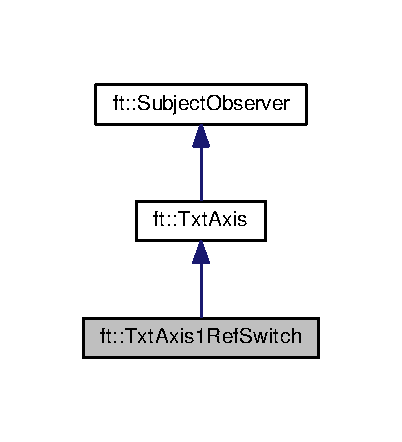
\includegraphics[width=193pt]{classft_1_1_txt_axis1_ref_switch__inherit__graph}
\end{center}
\end{figure}


Collaboration diagram for ft\+:\+:Txt\+Axis1\+Ref\+Switch\+:
\nopagebreak
\begin{figure}[H]
\begin{center}
\leavevmode
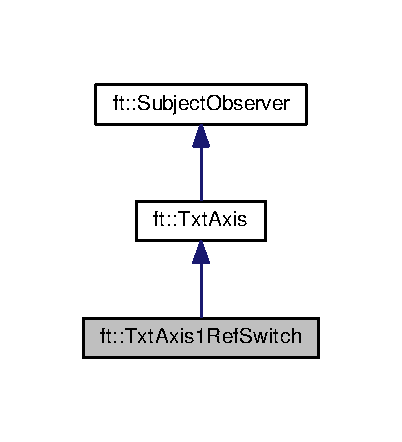
\includegraphics[width=193pt]{classft_1_1_txt_axis1_ref_switch__coll__graph}
\end{center}
\end{figure}
\subsection*{Public Member Functions}
\begin{DoxyCompactItemize}
\item 
\hyperlink{classft_1_1_txt_axis1_ref_switch_ac609b45e7b39e1807268780d6693019b}{Txt\+Axis1\+Ref\+Switch} (std\+::string \hyperlink{classft_1_1_txt_axis_a358af2b2ed1709b40ab6c9768c2795ef}{name}, F\+I\+S\+H\+\_\+\+X1\+\_\+\+T\+R\+A\+N\+S\+F\+ER $\ast$\hyperlink{classft_1_1_txt_axis_ae5521c2eda7b80599ed6340f6a8192f2}{p\+T\+Area}, uint8\+\_\+t \hyperlink{classft_1_1_txt_axis_a3a8988acb2f578fe96312221205c50c4}{chM}, uint8\+\_\+t \hyperlink{classft_1_1_txt_axis_a9b155580a8dcc876c8e0c4b9c92041e7}{ch\+S1}, uint16\+\_\+t \hyperlink{classft_1_1_txt_axis1_ref_switch_a8b9bda2c9ff12ef5f1355d630136e48b}{pos\+End})
\item 
virtual \hyperlink{classft_1_1_txt_axis1_ref_switch_a908594d73ac8b51867b3e2e21616f2be}{$\sim$\+Txt\+Axis1\+Ref\+Switch} ()
\item 
bool \hyperlink{classft_1_1_txt_axis1_ref_switch_a631984bd9524721f1338e1196a2510e5}{move\+Abs} (uint16\+\_\+t)
\item 
uint16\+\_\+t \hyperlink{classft_1_1_txt_axis1_ref_switch_aac2e9702b89ffb55fefad69bb24274c2}{get\+Pos\+End} ()
\end{DoxyCompactItemize}
\subsection*{Protected Member Functions}
\begin{DoxyCompactItemize}
\item 
virtual void \hyperlink{classft_1_1_txt_axis1_ref_switch_afbdf212009e8b29b67e01af18d708607}{set\+Motor\+Right} ()
\item 
virtual void \hyperlink{classft_1_1_txt_axis1_ref_switch_aef61418eee7beff5c8823d867188ad3b}{move\+Right} (uint16\+\_\+t steps, uint16\+\_\+t $\ast$p\+Pos)
\end{DoxyCompactItemize}
\subsection*{Protected Attributes}
\begin{DoxyCompactItemize}
\item 
uint16\+\_\+t \hyperlink{classft_1_1_txt_axis1_ref_switch_a8b9bda2c9ff12ef5f1355d630136e48b}{pos\+End}
\end{DoxyCompactItemize}
\subsection*{Friends}
\begin{DoxyCompactItemize}
\item 
class \hyperlink{classft_1_1_txt_axis1_ref_switch_aea03938f89578033a66fa5dba1f9fe09}{Txt\+Vacuum\+Gripper\+Robot}
\item 
class \hyperlink{classft_1_1_txt_axis1_ref_switch_ae0c44dc668d7ae80ecedb8484adf9fdf}{Txt\+High\+Bay\+Warehouse}
\end{DoxyCompactItemize}


\subsection{Constructor \& Destructor Documentation}
\index{ft\+::\+Txt\+Axis1\+Ref\+Switch@{ft\+::\+Txt\+Axis1\+Ref\+Switch}!Txt\+Axis1\+Ref\+Switch@{Txt\+Axis1\+Ref\+Switch}}
\index{Txt\+Axis1\+Ref\+Switch@{Txt\+Axis1\+Ref\+Switch}!ft\+::\+Txt\+Axis1\+Ref\+Switch@{ft\+::\+Txt\+Axis1\+Ref\+Switch}}
\subsubsection[{\texorpdfstring{Txt\+Axis1\+Ref\+Switch(std\+::string name, F\+I\+S\+H\+\_\+\+X1\+\_\+\+T\+R\+A\+N\+S\+F\+E\+R $\ast$p\+T\+Area, uint8\+\_\+t ch\+M, uint8\+\_\+t ch\+S1, uint16\+\_\+t pos\+End)}{TxtAxis1RefSwitch(std::string name, FISH_X1_TRANSFER *pTArea, uint8_t chM, uint8_t chS1, uint16_t posEnd)}}]{\setlength{\rightskip}{0pt plus 5cm}ft\+::\+Txt\+Axis1\+Ref\+Switch\+::\+Txt\+Axis1\+Ref\+Switch (
\begin{DoxyParamCaption}
\item[{std\+::string}]{name, }
\item[{F\+I\+S\+H\+\_\+\+X1\+\_\+\+T\+R\+A\+N\+S\+F\+ER $\ast$}]{p\+T\+Area, }
\item[{uint8\+\_\+t}]{chM, }
\item[{uint8\+\_\+t}]{ch\+S1, }
\item[{uint16\+\_\+t}]{pos\+End}
\end{DoxyParamCaption}
)}\hypertarget{classft_1_1_txt_axis1_ref_switch_ac609b45e7b39e1807268780d6693019b}{}\label{classft_1_1_txt_axis1_ref_switch_ac609b45e7b39e1807268780d6693019b}
\index{ft\+::\+Txt\+Axis1\+Ref\+Switch@{ft\+::\+Txt\+Axis1\+Ref\+Switch}!````~Txt\+Axis1\+Ref\+Switch@{$\sim$\+Txt\+Axis1\+Ref\+Switch}}
\index{````~Txt\+Axis1\+Ref\+Switch@{$\sim$\+Txt\+Axis1\+Ref\+Switch}!ft\+::\+Txt\+Axis1\+Ref\+Switch@{ft\+::\+Txt\+Axis1\+Ref\+Switch}}
\subsubsection[{\texorpdfstring{$\sim$\+Txt\+Axis1\+Ref\+Switch()}{~TxtAxis1RefSwitch()}}]{\setlength{\rightskip}{0pt plus 5cm}virtual ft\+::\+Txt\+Axis1\+Ref\+Switch\+::$\sim$\+Txt\+Axis1\+Ref\+Switch (
\begin{DoxyParamCaption}
{}
\end{DoxyParamCaption}
)\hspace{0.3cm}{\ttfamily [virtual]}}\hypertarget{classft_1_1_txt_axis1_ref_switch_a908594d73ac8b51867b3e2e21616f2be}{}\label{classft_1_1_txt_axis1_ref_switch_a908594d73ac8b51867b3e2e21616f2be}


\subsection{Member Function Documentation}
\index{ft\+::\+Txt\+Axis1\+Ref\+Switch@{ft\+::\+Txt\+Axis1\+Ref\+Switch}!get\+Pos\+End@{get\+Pos\+End}}
\index{get\+Pos\+End@{get\+Pos\+End}!ft\+::\+Txt\+Axis1\+Ref\+Switch@{ft\+::\+Txt\+Axis1\+Ref\+Switch}}
\subsubsection[{\texorpdfstring{get\+Pos\+End()}{getPosEnd()}}]{\setlength{\rightskip}{0pt plus 5cm}uint16\+\_\+t ft\+::\+Txt\+Axis1\+Ref\+Switch\+::get\+Pos\+End (
\begin{DoxyParamCaption}
{}
\end{DoxyParamCaption}
)\hspace{0.3cm}{\ttfamily [inline]}}\hypertarget{classft_1_1_txt_axis1_ref_switch_aac2e9702b89ffb55fefad69bb24274c2}{}\label{classft_1_1_txt_axis1_ref_switch_aac2e9702b89ffb55fefad69bb24274c2}
\index{ft\+::\+Txt\+Axis1\+Ref\+Switch@{ft\+::\+Txt\+Axis1\+Ref\+Switch}!move\+Abs@{move\+Abs}}
\index{move\+Abs@{move\+Abs}!ft\+::\+Txt\+Axis1\+Ref\+Switch@{ft\+::\+Txt\+Axis1\+Ref\+Switch}}
\subsubsection[{\texorpdfstring{move\+Abs(uint16\+\_\+t)}{moveAbs(uint16_t)}}]{\setlength{\rightskip}{0pt plus 5cm}bool ft\+::\+Txt\+Axis1\+Ref\+Switch\+::move\+Abs (
\begin{DoxyParamCaption}
\item[{uint16\+\_\+t}]{}
\end{DoxyParamCaption}
)\hspace{0.3cm}{\ttfamily [virtual]}}\hypertarget{classft_1_1_txt_axis1_ref_switch_a631984bd9524721f1338e1196a2510e5}{}\label{classft_1_1_txt_axis1_ref_switch_a631984bd9524721f1338e1196a2510e5}


Reimplemented from \hyperlink{classft_1_1_txt_axis_a0ae92e37ed640f5d65e59cd1ae6fe9cf}{ft\+::\+Txt\+Axis}.

\index{ft\+::\+Txt\+Axis1\+Ref\+Switch@{ft\+::\+Txt\+Axis1\+Ref\+Switch}!move\+Right@{move\+Right}}
\index{move\+Right@{move\+Right}!ft\+::\+Txt\+Axis1\+Ref\+Switch@{ft\+::\+Txt\+Axis1\+Ref\+Switch}}
\subsubsection[{\texorpdfstring{move\+Right(uint16\+\_\+t steps, uint16\+\_\+t $\ast$p\+Pos)}{moveRight(uint16_t steps, uint16_t *pPos)}}]{\setlength{\rightskip}{0pt plus 5cm}virtual void ft\+::\+Txt\+Axis1\+Ref\+Switch\+::move\+Right (
\begin{DoxyParamCaption}
\item[{uint16\+\_\+t}]{steps, }
\item[{uint16\+\_\+t $\ast$}]{p\+Pos}
\end{DoxyParamCaption}
)\hspace{0.3cm}{\ttfamily [protected]}, {\ttfamily [virtual]}}\hypertarget{classft_1_1_txt_axis1_ref_switch_aef61418eee7beff5c8823d867188ad3b}{}\label{classft_1_1_txt_axis1_ref_switch_aef61418eee7beff5c8823d867188ad3b}


Implements \hyperlink{classft_1_1_txt_axis_aac0aaaa04969160f42542e76057ccb75}{ft\+::\+Txt\+Axis}.

\index{ft\+::\+Txt\+Axis1\+Ref\+Switch@{ft\+::\+Txt\+Axis1\+Ref\+Switch}!set\+Motor\+Right@{set\+Motor\+Right}}
\index{set\+Motor\+Right@{set\+Motor\+Right}!ft\+::\+Txt\+Axis1\+Ref\+Switch@{ft\+::\+Txt\+Axis1\+Ref\+Switch}}
\subsubsection[{\texorpdfstring{set\+Motor\+Right()}{setMotorRight()}}]{\setlength{\rightskip}{0pt plus 5cm}virtual void ft\+::\+Txt\+Axis1\+Ref\+Switch\+::set\+Motor\+Right (
\begin{DoxyParamCaption}
{}
\end{DoxyParamCaption}
)\hspace{0.3cm}{\ttfamily [protected]}, {\ttfamily [virtual]}}\hypertarget{classft_1_1_txt_axis1_ref_switch_afbdf212009e8b29b67e01af18d708607}{}\label{classft_1_1_txt_axis1_ref_switch_afbdf212009e8b29b67e01af18d708607}


\subsection{Friends And Related Function Documentation}
\index{ft\+::\+Txt\+Axis1\+Ref\+Switch@{ft\+::\+Txt\+Axis1\+Ref\+Switch}!Txt\+High\+Bay\+Warehouse@{Txt\+High\+Bay\+Warehouse}}
\index{Txt\+High\+Bay\+Warehouse@{Txt\+High\+Bay\+Warehouse}!ft\+::\+Txt\+Axis1\+Ref\+Switch@{ft\+::\+Txt\+Axis1\+Ref\+Switch}}
\subsubsection[{\texorpdfstring{Txt\+High\+Bay\+Warehouse}{TxtHighBayWarehouse}}]{\setlength{\rightskip}{0pt plus 5cm}friend class {\bf Txt\+High\+Bay\+Warehouse}\hspace{0.3cm}{\ttfamily [friend]}}\hypertarget{classft_1_1_txt_axis1_ref_switch_ae0c44dc668d7ae80ecedb8484adf9fdf}{}\label{classft_1_1_txt_axis1_ref_switch_ae0c44dc668d7ae80ecedb8484adf9fdf}
\index{ft\+::\+Txt\+Axis1\+Ref\+Switch@{ft\+::\+Txt\+Axis1\+Ref\+Switch}!Txt\+Vacuum\+Gripper\+Robot@{Txt\+Vacuum\+Gripper\+Robot}}
\index{Txt\+Vacuum\+Gripper\+Robot@{Txt\+Vacuum\+Gripper\+Robot}!ft\+::\+Txt\+Axis1\+Ref\+Switch@{ft\+::\+Txt\+Axis1\+Ref\+Switch}}
\subsubsection[{\texorpdfstring{Txt\+Vacuum\+Gripper\+Robot}{TxtVacuumGripperRobot}}]{\setlength{\rightskip}{0pt plus 5cm}friend class {\bf Txt\+Vacuum\+Gripper\+Robot}\hspace{0.3cm}{\ttfamily [friend]}}\hypertarget{classft_1_1_txt_axis1_ref_switch_aea03938f89578033a66fa5dba1f9fe09}{}\label{classft_1_1_txt_axis1_ref_switch_aea03938f89578033a66fa5dba1f9fe09}


\subsection{Member Data Documentation}
\index{ft\+::\+Txt\+Axis1\+Ref\+Switch@{ft\+::\+Txt\+Axis1\+Ref\+Switch}!pos\+End@{pos\+End}}
\index{pos\+End@{pos\+End}!ft\+::\+Txt\+Axis1\+Ref\+Switch@{ft\+::\+Txt\+Axis1\+Ref\+Switch}}
\subsubsection[{\texorpdfstring{pos\+End}{posEnd}}]{\setlength{\rightskip}{0pt plus 5cm}uint16\+\_\+t ft\+::\+Txt\+Axis1\+Ref\+Switch\+::pos\+End\hspace{0.3cm}{\ttfamily [protected]}}\hypertarget{classft_1_1_txt_axis1_ref_switch_a8b9bda2c9ff12ef5f1355d630136e48b}{}\label{classft_1_1_txt_axis1_ref_switch_a8b9bda2c9ff12ef5f1355d630136e48b}


The documentation for this class was generated from the following file\+:\begin{DoxyCompactItemize}
\item 
\hyperlink{_txt_axis1_ref_switch_8h}{Txt\+Axis1\+Ref\+Switch.\+h}\end{DoxyCompactItemize}

\hypertarget{classft_1_1_txt_axis_n_ref_switch}{}\section{ft\+:\+:Txt\+Axis\+N\+Ref\+Switch Class Reference}
\label{classft_1_1_txt_axis_n_ref_switch}\index{ft\+::\+Txt\+Axis\+N\+Ref\+Switch@{ft\+::\+Txt\+Axis\+N\+Ref\+Switch}}


{\ttfamily \#include $<$Txt\+Axis\+N\+Ref\+Switch.\+h$>$}



Inheritance diagram for ft\+:\+:Txt\+Axis\+N\+Ref\+Switch\+:
\nopagebreak
\begin{figure}[H]
\begin{center}
\leavevmode
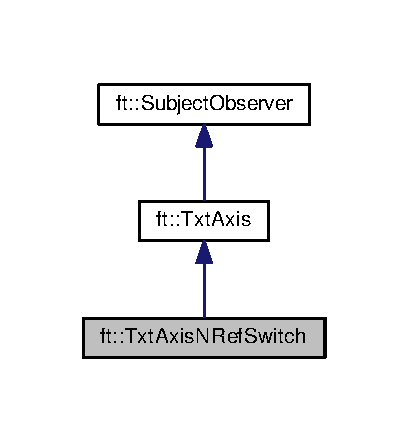
\includegraphics[width=196pt]{classft_1_1_txt_axis_n_ref_switch__inherit__graph}
\end{center}
\end{figure}


Collaboration diagram for ft\+:\+:Txt\+Axis\+N\+Ref\+Switch\+:
\nopagebreak
\begin{figure}[H]
\begin{center}
\leavevmode
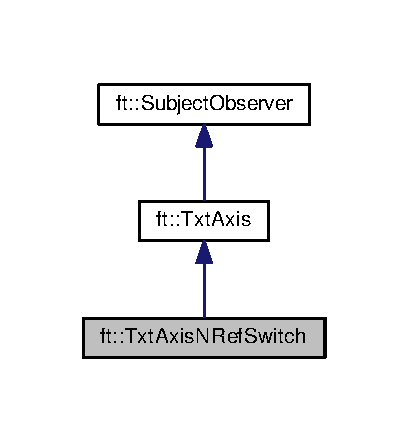
\includegraphics[width=196pt]{classft_1_1_txt_axis_n_ref_switch__coll__graph}
\end{center}
\end{figure}
\subsection*{Public Member Functions}
\begin{DoxyCompactItemize}
\item 
\hyperlink{classft_1_1_txt_axis_n_ref_switch_a614a6e2df3c9e575faedd582321e08d2}{Txt\+Axis\+N\+Ref\+Switch} (std\+::string \hyperlink{classft_1_1_txt_axis_a358af2b2ed1709b40ab6c9768c2795ef}{name}, F\+I\+S\+H\+\_\+\+X1\+\_\+\+T\+R\+A\+N\+S\+F\+ER $\ast$\hyperlink{classft_1_1_txt_axis_ae5521c2eda7b80599ed6340f6a8192f2}{p\+T\+Area}, uint8\+\_\+t \hyperlink{classft_1_1_txt_axis_a3a8988acb2f578fe96312221205c50c4}{chM}, uint8\+\_\+t \hyperlink{classft_1_1_txt_axis_a9b155580a8dcc876c8e0c4b9c92041e7}{ch\+S1}, uint8\+\_\+t ch\+S2)
\item 
\hyperlink{classft_1_1_txt_axis_n_ref_switch_ab27b2a2b57e61bd9e5f85e3b4d31d74e}{Txt\+Axis\+N\+Ref\+Switch} (std\+::string \hyperlink{classft_1_1_txt_axis_a358af2b2ed1709b40ab6c9768c2795ef}{name}, F\+I\+S\+H\+\_\+\+X1\+\_\+\+T\+R\+A\+N\+S\+F\+ER $\ast$\hyperlink{classft_1_1_txt_axis_ae5521c2eda7b80599ed6340f6a8192f2}{p\+T\+Area}, uint8\+\_\+t \hyperlink{classft_1_1_txt_axis_a3a8988acb2f578fe96312221205c50c4}{chM}, uint8\+\_\+t \hyperlink{classft_1_1_txt_axis_a9b155580a8dcc876c8e0c4b9c92041e7}{ch\+S1}, uint8\+\_\+t ch\+S2, uint8\+\_\+t ch\+S3)
\item 
virtual \hyperlink{classft_1_1_txt_axis_n_ref_switch_a559cde62e5b9192fd634216ec1921801}{$\sim$\+Txt\+Axis\+N\+Ref\+Switch} ()
\item 
void \hyperlink{classft_1_1_txt_axis_n_ref_switch_aa663559c3da6e40a21185cfc4e6c573c}{move\+S2X} (int idx)
\item 
void \hyperlink{classft_1_1_txt_axis_n_ref_switch_aaee4c0ac6d1379639c40588ac3d58c63}{move\+S2} ()
\item 
std\+::thread \hyperlink{classft_1_1_txt_axis_n_ref_switch_a9152452c5b6f75b293ad83510e537cf4}{move\+S2\+Thread} ()
\item 
void \hyperlink{classft_1_1_txt_axis_n_ref_switch_a91a91446c84f2e6be47394ada3c3de0c}{move\+S3} ()
\item 
std\+::thread \hyperlink{classft_1_1_txt_axis_n_ref_switch_a6abe7590af5db9c355fe7a263f5a787b}{move\+S3\+Thread} ()
\item 
bool \hyperlink{classft_1_1_txt_axis_n_ref_switch_abc4e26eee2563496af18d107aef1b38d}{is\+S2\+X\+Valid} (int idx)
\end{DoxyCompactItemize}
\subsection*{Protected Member Functions}
\begin{DoxyCompactItemize}
\item 
virtual void \hyperlink{classft_1_1_txt_axis_n_ref_switch_ae4938459dbc75af81d58aa3a2075baf4}{set\+Motor\+Right} ()
\item 
virtual void \hyperlink{classft_1_1_txt_axis_n_ref_switch_ae8bf5d862cabf4598371ebbbaa67a4f0}{move\+Right} (uint16\+\_\+t steps, uint16\+\_\+t $\ast$p\+Pos)
\end{DoxyCompactItemize}
\subsection*{Protected Attributes}
\begin{DoxyCompactItemize}
\item 
std\+::vector$<$ uint8\+\_\+t $>$ \hyperlink{classft_1_1_txt_axis_n_ref_switch_a36c2c99525ecda394e43472cb9bfd4a7}{ch\+S2X}
\end{DoxyCompactItemize}
\subsection*{Friends}
\begin{DoxyCompactItemize}
\item 
class \hyperlink{classft_1_1_txt_axis_n_ref_switch_aea03938f89578033a66fa5dba1f9fe09}{Txt\+Vacuum\+Gripper\+Robot}
\item 
class \hyperlink{classft_1_1_txt_axis_n_ref_switch_ae0c44dc668d7ae80ecedb8484adf9fdf}{Txt\+High\+Bay\+Warehouse}
\end{DoxyCompactItemize}


\subsection{Constructor \& Destructor Documentation}
\index{ft\+::\+Txt\+Axis\+N\+Ref\+Switch@{ft\+::\+Txt\+Axis\+N\+Ref\+Switch}!Txt\+Axis\+N\+Ref\+Switch@{Txt\+Axis\+N\+Ref\+Switch}}
\index{Txt\+Axis\+N\+Ref\+Switch@{Txt\+Axis\+N\+Ref\+Switch}!ft\+::\+Txt\+Axis\+N\+Ref\+Switch@{ft\+::\+Txt\+Axis\+N\+Ref\+Switch}}
\subsubsection[{\texorpdfstring{Txt\+Axis\+N\+Ref\+Switch(std\+::string name, F\+I\+S\+H\+\_\+\+X1\+\_\+\+T\+R\+A\+N\+S\+F\+E\+R $\ast$p\+T\+Area, uint8\+\_\+t ch\+M, uint8\+\_\+t ch\+S1, uint8\+\_\+t ch\+S2)}{TxtAxisNRefSwitch(std::string name, FISH_X1_TRANSFER *pTArea, uint8_t chM, uint8_t chS1, uint8_t chS2)}}]{\setlength{\rightskip}{0pt plus 5cm}ft\+::\+Txt\+Axis\+N\+Ref\+Switch\+::\+Txt\+Axis\+N\+Ref\+Switch (
\begin{DoxyParamCaption}
\item[{std\+::string}]{name, }
\item[{F\+I\+S\+H\+\_\+\+X1\+\_\+\+T\+R\+A\+N\+S\+F\+ER $\ast$}]{p\+T\+Area, }
\item[{uint8\+\_\+t}]{chM, }
\item[{uint8\+\_\+t}]{ch\+S1, }
\item[{uint8\+\_\+t}]{ch\+S2}
\end{DoxyParamCaption}
)}\hypertarget{classft_1_1_txt_axis_n_ref_switch_a614a6e2df3c9e575faedd582321e08d2}{}\label{classft_1_1_txt_axis_n_ref_switch_a614a6e2df3c9e575faedd582321e08d2}
\index{ft\+::\+Txt\+Axis\+N\+Ref\+Switch@{ft\+::\+Txt\+Axis\+N\+Ref\+Switch}!Txt\+Axis\+N\+Ref\+Switch@{Txt\+Axis\+N\+Ref\+Switch}}
\index{Txt\+Axis\+N\+Ref\+Switch@{Txt\+Axis\+N\+Ref\+Switch}!ft\+::\+Txt\+Axis\+N\+Ref\+Switch@{ft\+::\+Txt\+Axis\+N\+Ref\+Switch}}
\subsubsection[{\texorpdfstring{Txt\+Axis\+N\+Ref\+Switch(std\+::string name, F\+I\+S\+H\+\_\+\+X1\+\_\+\+T\+R\+A\+N\+S\+F\+E\+R $\ast$p\+T\+Area, uint8\+\_\+t ch\+M, uint8\+\_\+t ch\+S1, uint8\+\_\+t ch\+S2, uint8\+\_\+t ch\+S3)}{TxtAxisNRefSwitch(std::string name, FISH_X1_TRANSFER *pTArea, uint8_t chM, uint8_t chS1, uint8_t chS2, uint8_t chS3)}}]{\setlength{\rightskip}{0pt plus 5cm}ft\+::\+Txt\+Axis\+N\+Ref\+Switch\+::\+Txt\+Axis\+N\+Ref\+Switch (
\begin{DoxyParamCaption}
\item[{std\+::string}]{name, }
\item[{F\+I\+S\+H\+\_\+\+X1\+\_\+\+T\+R\+A\+N\+S\+F\+ER $\ast$}]{p\+T\+Area, }
\item[{uint8\+\_\+t}]{chM, }
\item[{uint8\+\_\+t}]{ch\+S1, }
\item[{uint8\+\_\+t}]{ch\+S2, }
\item[{uint8\+\_\+t}]{ch\+S3}
\end{DoxyParamCaption}
)}\hypertarget{classft_1_1_txt_axis_n_ref_switch_ab27b2a2b57e61bd9e5f85e3b4d31d74e}{}\label{classft_1_1_txt_axis_n_ref_switch_ab27b2a2b57e61bd9e5f85e3b4d31d74e}
\index{ft\+::\+Txt\+Axis\+N\+Ref\+Switch@{ft\+::\+Txt\+Axis\+N\+Ref\+Switch}!````~Txt\+Axis\+N\+Ref\+Switch@{$\sim$\+Txt\+Axis\+N\+Ref\+Switch}}
\index{````~Txt\+Axis\+N\+Ref\+Switch@{$\sim$\+Txt\+Axis\+N\+Ref\+Switch}!ft\+::\+Txt\+Axis\+N\+Ref\+Switch@{ft\+::\+Txt\+Axis\+N\+Ref\+Switch}}
\subsubsection[{\texorpdfstring{$\sim$\+Txt\+Axis\+N\+Ref\+Switch()}{~TxtAxisNRefSwitch()}}]{\setlength{\rightskip}{0pt plus 5cm}virtual ft\+::\+Txt\+Axis\+N\+Ref\+Switch\+::$\sim$\+Txt\+Axis\+N\+Ref\+Switch (
\begin{DoxyParamCaption}
{}
\end{DoxyParamCaption}
)\hspace{0.3cm}{\ttfamily [virtual]}}\hypertarget{classft_1_1_txt_axis_n_ref_switch_a559cde62e5b9192fd634216ec1921801}{}\label{classft_1_1_txt_axis_n_ref_switch_a559cde62e5b9192fd634216ec1921801}


\subsection{Member Function Documentation}
\index{ft\+::\+Txt\+Axis\+N\+Ref\+Switch@{ft\+::\+Txt\+Axis\+N\+Ref\+Switch}!is\+S2\+X\+Valid@{is\+S2\+X\+Valid}}
\index{is\+S2\+X\+Valid@{is\+S2\+X\+Valid}!ft\+::\+Txt\+Axis\+N\+Ref\+Switch@{ft\+::\+Txt\+Axis\+N\+Ref\+Switch}}
\subsubsection[{\texorpdfstring{is\+S2\+X\+Valid(int idx)}{isS2XValid(int idx)}}]{\setlength{\rightskip}{0pt plus 5cm}bool ft\+::\+Txt\+Axis\+N\+Ref\+Switch\+::is\+S2\+X\+Valid (
\begin{DoxyParamCaption}
\item[{int}]{idx}
\end{DoxyParamCaption}
)\hspace{0.3cm}{\ttfamily [inline]}}\hypertarget{classft_1_1_txt_axis_n_ref_switch_abc4e26eee2563496af18d107aef1b38d}{}\label{classft_1_1_txt_axis_n_ref_switch_abc4e26eee2563496af18d107aef1b38d}
\index{ft\+::\+Txt\+Axis\+N\+Ref\+Switch@{ft\+::\+Txt\+Axis\+N\+Ref\+Switch}!move\+Right@{move\+Right}}
\index{move\+Right@{move\+Right}!ft\+::\+Txt\+Axis\+N\+Ref\+Switch@{ft\+::\+Txt\+Axis\+N\+Ref\+Switch}}
\subsubsection[{\texorpdfstring{move\+Right(uint16\+\_\+t steps, uint16\+\_\+t $\ast$p\+Pos)}{moveRight(uint16_t steps, uint16_t *pPos)}}]{\setlength{\rightskip}{0pt plus 5cm}virtual void ft\+::\+Txt\+Axis\+N\+Ref\+Switch\+::move\+Right (
\begin{DoxyParamCaption}
\item[{uint16\+\_\+t}]{steps, }
\item[{uint16\+\_\+t $\ast$}]{p\+Pos}
\end{DoxyParamCaption}
)\hspace{0.3cm}{\ttfamily [protected]}, {\ttfamily [virtual]}}\hypertarget{classft_1_1_txt_axis_n_ref_switch_ae8bf5d862cabf4598371ebbbaa67a4f0}{}\label{classft_1_1_txt_axis_n_ref_switch_ae8bf5d862cabf4598371ebbbaa67a4f0}


Implements \hyperlink{classft_1_1_txt_axis_aac0aaaa04969160f42542e76057ccb75}{ft\+::\+Txt\+Axis}.

\index{ft\+::\+Txt\+Axis\+N\+Ref\+Switch@{ft\+::\+Txt\+Axis\+N\+Ref\+Switch}!move\+S2@{move\+S2}}
\index{move\+S2@{move\+S2}!ft\+::\+Txt\+Axis\+N\+Ref\+Switch@{ft\+::\+Txt\+Axis\+N\+Ref\+Switch}}
\subsubsection[{\texorpdfstring{move\+S2()}{moveS2()}}]{\setlength{\rightskip}{0pt plus 5cm}void ft\+::\+Txt\+Axis\+N\+Ref\+Switch\+::move\+S2 (
\begin{DoxyParamCaption}
{}
\end{DoxyParamCaption}
)\hspace{0.3cm}{\ttfamily [inline]}}\hypertarget{classft_1_1_txt_axis_n_ref_switch_aaee4c0ac6d1379639c40588ac3d58c63}{}\label{classft_1_1_txt_axis_n_ref_switch_aaee4c0ac6d1379639c40588ac3d58c63}
\index{ft\+::\+Txt\+Axis\+N\+Ref\+Switch@{ft\+::\+Txt\+Axis\+N\+Ref\+Switch}!move\+S2\+Thread@{move\+S2\+Thread}}
\index{move\+S2\+Thread@{move\+S2\+Thread}!ft\+::\+Txt\+Axis\+N\+Ref\+Switch@{ft\+::\+Txt\+Axis\+N\+Ref\+Switch}}
\subsubsection[{\texorpdfstring{move\+S2\+Thread()}{moveS2Thread()}}]{\setlength{\rightskip}{0pt plus 5cm}std\+::thread ft\+::\+Txt\+Axis\+N\+Ref\+Switch\+::move\+S2\+Thread (
\begin{DoxyParamCaption}
{}
\end{DoxyParamCaption}
)\hspace{0.3cm}{\ttfamily [inline]}}\hypertarget{classft_1_1_txt_axis_n_ref_switch_a9152452c5b6f75b293ad83510e537cf4}{}\label{classft_1_1_txt_axis_n_ref_switch_a9152452c5b6f75b293ad83510e537cf4}
\index{ft\+::\+Txt\+Axis\+N\+Ref\+Switch@{ft\+::\+Txt\+Axis\+N\+Ref\+Switch}!move\+S2X@{move\+S2X}}
\index{move\+S2X@{move\+S2X}!ft\+::\+Txt\+Axis\+N\+Ref\+Switch@{ft\+::\+Txt\+Axis\+N\+Ref\+Switch}}
\subsubsection[{\texorpdfstring{move\+S2\+X(int idx)}{moveS2X(int idx)}}]{\setlength{\rightskip}{0pt plus 5cm}void ft\+::\+Txt\+Axis\+N\+Ref\+Switch\+::move\+S2X (
\begin{DoxyParamCaption}
\item[{int}]{idx}
\end{DoxyParamCaption}
)}\hypertarget{classft_1_1_txt_axis_n_ref_switch_aa663559c3da6e40a21185cfc4e6c573c}{}\label{classft_1_1_txt_axis_n_ref_switch_aa663559c3da6e40a21185cfc4e6c573c}
\index{ft\+::\+Txt\+Axis\+N\+Ref\+Switch@{ft\+::\+Txt\+Axis\+N\+Ref\+Switch}!move\+S3@{move\+S3}}
\index{move\+S3@{move\+S3}!ft\+::\+Txt\+Axis\+N\+Ref\+Switch@{ft\+::\+Txt\+Axis\+N\+Ref\+Switch}}
\subsubsection[{\texorpdfstring{move\+S3()}{moveS3()}}]{\setlength{\rightskip}{0pt plus 5cm}void ft\+::\+Txt\+Axis\+N\+Ref\+Switch\+::move\+S3 (
\begin{DoxyParamCaption}
{}
\end{DoxyParamCaption}
)\hspace{0.3cm}{\ttfamily [inline]}}\hypertarget{classft_1_1_txt_axis_n_ref_switch_a91a91446c84f2e6be47394ada3c3de0c}{}\label{classft_1_1_txt_axis_n_ref_switch_a91a91446c84f2e6be47394ada3c3de0c}
\index{ft\+::\+Txt\+Axis\+N\+Ref\+Switch@{ft\+::\+Txt\+Axis\+N\+Ref\+Switch}!move\+S3\+Thread@{move\+S3\+Thread}}
\index{move\+S3\+Thread@{move\+S3\+Thread}!ft\+::\+Txt\+Axis\+N\+Ref\+Switch@{ft\+::\+Txt\+Axis\+N\+Ref\+Switch}}
\subsubsection[{\texorpdfstring{move\+S3\+Thread()}{moveS3Thread()}}]{\setlength{\rightskip}{0pt plus 5cm}std\+::thread ft\+::\+Txt\+Axis\+N\+Ref\+Switch\+::move\+S3\+Thread (
\begin{DoxyParamCaption}
{}
\end{DoxyParamCaption}
)\hspace{0.3cm}{\ttfamily [inline]}}\hypertarget{classft_1_1_txt_axis_n_ref_switch_a6abe7590af5db9c355fe7a263f5a787b}{}\label{classft_1_1_txt_axis_n_ref_switch_a6abe7590af5db9c355fe7a263f5a787b}
\index{ft\+::\+Txt\+Axis\+N\+Ref\+Switch@{ft\+::\+Txt\+Axis\+N\+Ref\+Switch}!set\+Motor\+Right@{set\+Motor\+Right}}
\index{set\+Motor\+Right@{set\+Motor\+Right}!ft\+::\+Txt\+Axis\+N\+Ref\+Switch@{ft\+::\+Txt\+Axis\+N\+Ref\+Switch}}
\subsubsection[{\texorpdfstring{set\+Motor\+Right()}{setMotorRight()}}]{\setlength{\rightskip}{0pt plus 5cm}virtual void ft\+::\+Txt\+Axis\+N\+Ref\+Switch\+::set\+Motor\+Right (
\begin{DoxyParamCaption}
{}
\end{DoxyParamCaption}
)\hspace{0.3cm}{\ttfamily [protected]}, {\ttfamily [virtual]}}\hypertarget{classft_1_1_txt_axis_n_ref_switch_ae4938459dbc75af81d58aa3a2075baf4}{}\label{classft_1_1_txt_axis_n_ref_switch_ae4938459dbc75af81d58aa3a2075baf4}


\subsection{Friends And Related Function Documentation}
\index{ft\+::\+Txt\+Axis\+N\+Ref\+Switch@{ft\+::\+Txt\+Axis\+N\+Ref\+Switch}!Txt\+High\+Bay\+Warehouse@{Txt\+High\+Bay\+Warehouse}}
\index{Txt\+High\+Bay\+Warehouse@{Txt\+High\+Bay\+Warehouse}!ft\+::\+Txt\+Axis\+N\+Ref\+Switch@{ft\+::\+Txt\+Axis\+N\+Ref\+Switch}}
\subsubsection[{\texorpdfstring{Txt\+High\+Bay\+Warehouse}{TxtHighBayWarehouse}}]{\setlength{\rightskip}{0pt plus 5cm}friend class {\bf Txt\+High\+Bay\+Warehouse}\hspace{0.3cm}{\ttfamily [friend]}}\hypertarget{classft_1_1_txt_axis_n_ref_switch_ae0c44dc668d7ae80ecedb8484adf9fdf}{}\label{classft_1_1_txt_axis_n_ref_switch_ae0c44dc668d7ae80ecedb8484adf9fdf}
\index{ft\+::\+Txt\+Axis\+N\+Ref\+Switch@{ft\+::\+Txt\+Axis\+N\+Ref\+Switch}!Txt\+Vacuum\+Gripper\+Robot@{Txt\+Vacuum\+Gripper\+Robot}}
\index{Txt\+Vacuum\+Gripper\+Robot@{Txt\+Vacuum\+Gripper\+Robot}!ft\+::\+Txt\+Axis\+N\+Ref\+Switch@{ft\+::\+Txt\+Axis\+N\+Ref\+Switch}}
\subsubsection[{\texorpdfstring{Txt\+Vacuum\+Gripper\+Robot}{TxtVacuumGripperRobot}}]{\setlength{\rightskip}{0pt plus 5cm}friend class {\bf Txt\+Vacuum\+Gripper\+Robot}\hspace{0.3cm}{\ttfamily [friend]}}\hypertarget{classft_1_1_txt_axis_n_ref_switch_aea03938f89578033a66fa5dba1f9fe09}{}\label{classft_1_1_txt_axis_n_ref_switch_aea03938f89578033a66fa5dba1f9fe09}


\subsection{Member Data Documentation}
\index{ft\+::\+Txt\+Axis\+N\+Ref\+Switch@{ft\+::\+Txt\+Axis\+N\+Ref\+Switch}!ch\+S2X@{ch\+S2X}}
\index{ch\+S2X@{ch\+S2X}!ft\+::\+Txt\+Axis\+N\+Ref\+Switch@{ft\+::\+Txt\+Axis\+N\+Ref\+Switch}}
\subsubsection[{\texorpdfstring{ch\+S2X}{chS2X}}]{\setlength{\rightskip}{0pt plus 5cm}std\+::vector$<$uint8\+\_\+t$>$ ft\+::\+Txt\+Axis\+N\+Ref\+Switch\+::ch\+S2X\hspace{0.3cm}{\ttfamily [protected]}}\hypertarget{classft_1_1_txt_axis_n_ref_switch_a36c2c99525ecda394e43472cb9bfd4a7}{}\label{classft_1_1_txt_axis_n_ref_switch_a36c2c99525ecda394e43472cb9bfd4a7}


The documentation for this class was generated from the following file\+:\begin{DoxyCompactItemize}
\item 
\hyperlink{_txt_axis_n_ref_switch_8h}{Txt\+Axis\+N\+Ref\+Switch.\+h}\end{DoxyCompactItemize}

\hypertarget{classft_1_1_txt_b_m_e680}{}\section{ft\+:\+:Txt\+B\+M\+E680 Class Reference}
\label{classft_1_1_txt_b_m_e680}\index{ft\+::\+Txt\+B\+M\+E680@{ft\+::\+Txt\+B\+M\+E680}}


{\ttfamily \#include $<$Txt\+B\+M\+E680.\+h$>$}



Inheritance diagram for ft\+:\+:Txt\+B\+M\+E680\+:
\nopagebreak
\begin{figure}[H]
\begin{center}
\leavevmode
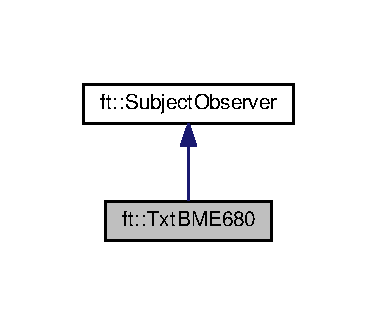
\includegraphics[width=181pt]{classft_1_1_txt_b_m_e680__inherit__graph}
\end{center}
\end{figure}


Collaboration diagram for ft\+:\+:Txt\+B\+M\+E680\+:
\nopagebreak
\begin{figure}[H]
\begin{center}
\leavevmode
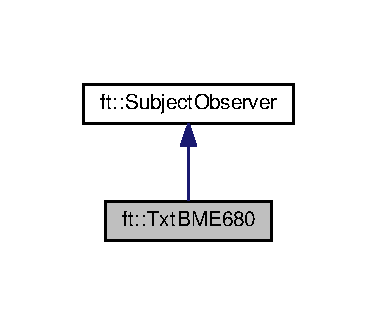
\includegraphics[width=181pt]{classft_1_1_txt_b_m_e680__coll__graph}
\end{center}
\end{figure}
\subsection*{Public Member Functions}
\begin{DoxyCompactItemize}
\item 
\hyperlink{classft_1_1_txt_b_m_e680_a51424e30b01f39e9e89799939782b7d3}{Txt\+B\+M\+E680} (float sample\+\_\+rate=B\+S\+E\+C\+\_\+\+S\+A\+M\+P\+L\+E\+\_\+\+R\+A\+T\+E\+\_\+\+LP, float temp\+\_\+offset=3.\+1f)
\item 
virtual \hyperlink{classft_1_1_txt_b_m_e680_a0b19a4ae70789f2c438b79e1a66b7663}{$\sim$\+Txt\+B\+M\+E680} ()
\item 
int \hyperlink{classft_1_1_txt_b_m_e680_ae06fb1fcb0180fb433fe7e79a6bf75b9}{init} ()
\item 
int \hyperlink{classft_1_1_txt_b_m_e680_a539a21a9fb7aac1ed5b2f36df542b5a3}{exit} ()
\end{DoxyCompactItemize}
\subsection*{Public Attributes}
\begin{DoxyCompactItemize}
\item 
int64\+\_\+t \hyperlink{classft_1_1_txt_b_m_e680_a783269ac820707b6902c839d148d582e}{\+\_\+timestamp} = 0
\item 
float \hyperlink{classft_1_1_txt_b_m_e680_ab4e4a74f8eafd99aaa956897389594ab}{\+\_\+iaq} = 0.f
\item 
uint8\+\_\+t \hyperlink{classft_1_1_txt_b_m_e680_a522ebe4c6d3baaa4f8cc96af9120ad04}{\+\_\+iaq\+\_\+accuracy} = 0
\item 
float \hyperlink{classft_1_1_txt_b_m_e680_ae810396be41cb787111ed00c4d1ef227}{\+\_\+temperature} = 0.f
\item 
float \hyperlink{classft_1_1_txt_b_m_e680_a890146594ddfb189f5f9d67373a1d60c}{\+\_\+humidity} = 0.f
\item 
float \hyperlink{classft_1_1_txt_b_m_e680_a5a70e308fa8a741a1ac97d7ae1aed449}{\+\_\+pressure} = 0.f
\item 
float \hyperlink{classft_1_1_txt_b_m_e680_a3fee3e0dc5cd6d47a0c86762cbfd6dc1}{\+\_\+raw\+\_\+temperature} = 0.f
\item 
float \hyperlink{classft_1_1_txt_b_m_e680_a4801e5e34a976e5771fe8a2ca20e0b78}{\+\_\+raw\+\_\+humidity} = 0.f
\item 
float \hyperlink{classft_1_1_txt_b_m_e680_a29ce3b76c378dac5e710c27b3f605e97}{\+\_\+gas} = 0.f
\end{DoxyCompactItemize}


\subsection{Constructor \& Destructor Documentation}
\index{ft\+::\+Txt\+B\+M\+E680@{ft\+::\+Txt\+B\+M\+E680}!Txt\+B\+M\+E680@{Txt\+B\+M\+E680}}
\index{Txt\+B\+M\+E680@{Txt\+B\+M\+E680}!ft\+::\+Txt\+B\+M\+E680@{ft\+::\+Txt\+B\+M\+E680}}
\subsubsection[{\texorpdfstring{Txt\+B\+M\+E680(float sample\+\_\+rate=\+B\+S\+E\+C\+\_\+\+S\+A\+M\+P\+L\+E\+\_\+\+R\+A\+T\+E\+\_\+\+L\+P, float temp\+\_\+offset=3.\+1f)}{TxtBME680(float sample_rate=BSEC_SAMPLE_RATE_LP, float temp_offset=3.1f)}}]{\setlength{\rightskip}{0pt plus 5cm}ft\+::\+Txt\+B\+M\+E680\+::\+Txt\+B\+M\+E680 (
\begin{DoxyParamCaption}
\item[{float}]{sample\+\_\+rate = {\ttfamily BSEC\+\_\+SAMPLE\+\_\+RATE\+\_\+LP}, }
\item[{float}]{temp\+\_\+offset = {\ttfamily 3.1f}}
\end{DoxyParamCaption}
)}\hypertarget{classft_1_1_txt_b_m_e680_a51424e30b01f39e9e89799939782b7d3}{}\label{classft_1_1_txt_b_m_e680_a51424e30b01f39e9e89799939782b7d3}
\index{ft\+::\+Txt\+B\+M\+E680@{ft\+::\+Txt\+B\+M\+E680}!````~Txt\+B\+M\+E680@{$\sim$\+Txt\+B\+M\+E680}}
\index{````~Txt\+B\+M\+E680@{$\sim$\+Txt\+B\+M\+E680}!ft\+::\+Txt\+B\+M\+E680@{ft\+::\+Txt\+B\+M\+E680}}
\subsubsection[{\texorpdfstring{$\sim$\+Txt\+B\+M\+E680()}{~TxtBME680()}}]{\setlength{\rightskip}{0pt plus 5cm}virtual ft\+::\+Txt\+B\+M\+E680\+::$\sim$\+Txt\+B\+M\+E680 (
\begin{DoxyParamCaption}
{}
\end{DoxyParamCaption}
)\hspace{0.3cm}{\ttfamily [virtual]}}\hypertarget{classft_1_1_txt_b_m_e680_a0b19a4ae70789f2c438b79e1a66b7663}{}\label{classft_1_1_txt_b_m_e680_a0b19a4ae70789f2c438b79e1a66b7663}


\subsection{Member Function Documentation}
\index{ft\+::\+Txt\+B\+M\+E680@{ft\+::\+Txt\+B\+M\+E680}!exit@{exit}}
\index{exit@{exit}!ft\+::\+Txt\+B\+M\+E680@{ft\+::\+Txt\+B\+M\+E680}}
\subsubsection[{\texorpdfstring{exit()}{exit()}}]{\setlength{\rightskip}{0pt plus 5cm}int ft\+::\+Txt\+B\+M\+E680\+::exit (
\begin{DoxyParamCaption}
{}
\end{DoxyParamCaption}
)}\hypertarget{classft_1_1_txt_b_m_e680_a539a21a9fb7aac1ed5b2f36df542b5a3}{}\label{classft_1_1_txt_b_m_e680_a539a21a9fb7aac1ed5b2f36df542b5a3}
\index{ft\+::\+Txt\+B\+M\+E680@{ft\+::\+Txt\+B\+M\+E680}!init@{init}}
\index{init@{init}!ft\+::\+Txt\+B\+M\+E680@{ft\+::\+Txt\+B\+M\+E680}}
\subsubsection[{\texorpdfstring{init()}{init()}}]{\setlength{\rightskip}{0pt plus 5cm}int ft\+::\+Txt\+B\+M\+E680\+::init (
\begin{DoxyParamCaption}
{}
\end{DoxyParamCaption}
)}\hypertarget{classft_1_1_txt_b_m_e680_ae06fb1fcb0180fb433fe7e79a6bf75b9}{}\label{classft_1_1_txt_b_m_e680_ae06fb1fcb0180fb433fe7e79a6bf75b9}


\subsection{Member Data Documentation}
\index{ft\+::\+Txt\+B\+M\+E680@{ft\+::\+Txt\+B\+M\+E680}!\+\_\+gas@{\+\_\+gas}}
\index{\+\_\+gas@{\+\_\+gas}!ft\+::\+Txt\+B\+M\+E680@{ft\+::\+Txt\+B\+M\+E680}}
\subsubsection[{\texorpdfstring{\+\_\+gas}{_gas}}]{\setlength{\rightskip}{0pt plus 5cm}float ft\+::\+Txt\+B\+M\+E680\+::\+\_\+gas = 0.f}\hypertarget{classft_1_1_txt_b_m_e680_a29ce3b76c378dac5e710c27b3f605e97}{}\label{classft_1_1_txt_b_m_e680_a29ce3b76c378dac5e710c27b3f605e97}
\index{ft\+::\+Txt\+B\+M\+E680@{ft\+::\+Txt\+B\+M\+E680}!\+\_\+humidity@{\+\_\+humidity}}
\index{\+\_\+humidity@{\+\_\+humidity}!ft\+::\+Txt\+B\+M\+E680@{ft\+::\+Txt\+B\+M\+E680}}
\subsubsection[{\texorpdfstring{\+\_\+humidity}{_humidity}}]{\setlength{\rightskip}{0pt plus 5cm}float ft\+::\+Txt\+B\+M\+E680\+::\+\_\+humidity = 0.f}\hypertarget{classft_1_1_txt_b_m_e680_a890146594ddfb189f5f9d67373a1d60c}{}\label{classft_1_1_txt_b_m_e680_a890146594ddfb189f5f9d67373a1d60c}
\index{ft\+::\+Txt\+B\+M\+E680@{ft\+::\+Txt\+B\+M\+E680}!\+\_\+iaq@{\+\_\+iaq}}
\index{\+\_\+iaq@{\+\_\+iaq}!ft\+::\+Txt\+B\+M\+E680@{ft\+::\+Txt\+B\+M\+E680}}
\subsubsection[{\texorpdfstring{\+\_\+iaq}{_iaq}}]{\setlength{\rightskip}{0pt plus 5cm}float ft\+::\+Txt\+B\+M\+E680\+::\+\_\+iaq = 0.f}\hypertarget{classft_1_1_txt_b_m_e680_ab4e4a74f8eafd99aaa956897389594ab}{}\label{classft_1_1_txt_b_m_e680_ab4e4a74f8eafd99aaa956897389594ab}
\index{ft\+::\+Txt\+B\+M\+E680@{ft\+::\+Txt\+B\+M\+E680}!\+\_\+iaq\+\_\+accuracy@{\+\_\+iaq\+\_\+accuracy}}
\index{\+\_\+iaq\+\_\+accuracy@{\+\_\+iaq\+\_\+accuracy}!ft\+::\+Txt\+B\+M\+E680@{ft\+::\+Txt\+B\+M\+E680}}
\subsubsection[{\texorpdfstring{\+\_\+iaq\+\_\+accuracy}{_iaq_accuracy}}]{\setlength{\rightskip}{0pt plus 5cm}uint8\+\_\+t ft\+::\+Txt\+B\+M\+E680\+::\+\_\+iaq\+\_\+accuracy = 0}\hypertarget{classft_1_1_txt_b_m_e680_a522ebe4c6d3baaa4f8cc96af9120ad04}{}\label{classft_1_1_txt_b_m_e680_a522ebe4c6d3baaa4f8cc96af9120ad04}
\index{ft\+::\+Txt\+B\+M\+E680@{ft\+::\+Txt\+B\+M\+E680}!\+\_\+pressure@{\+\_\+pressure}}
\index{\+\_\+pressure@{\+\_\+pressure}!ft\+::\+Txt\+B\+M\+E680@{ft\+::\+Txt\+B\+M\+E680}}
\subsubsection[{\texorpdfstring{\+\_\+pressure}{_pressure}}]{\setlength{\rightskip}{0pt plus 5cm}float ft\+::\+Txt\+B\+M\+E680\+::\+\_\+pressure = 0.f}\hypertarget{classft_1_1_txt_b_m_e680_a5a70e308fa8a741a1ac97d7ae1aed449}{}\label{classft_1_1_txt_b_m_e680_a5a70e308fa8a741a1ac97d7ae1aed449}
\index{ft\+::\+Txt\+B\+M\+E680@{ft\+::\+Txt\+B\+M\+E680}!\+\_\+raw\+\_\+humidity@{\+\_\+raw\+\_\+humidity}}
\index{\+\_\+raw\+\_\+humidity@{\+\_\+raw\+\_\+humidity}!ft\+::\+Txt\+B\+M\+E680@{ft\+::\+Txt\+B\+M\+E680}}
\subsubsection[{\texorpdfstring{\+\_\+raw\+\_\+humidity}{_raw_humidity}}]{\setlength{\rightskip}{0pt plus 5cm}float ft\+::\+Txt\+B\+M\+E680\+::\+\_\+raw\+\_\+humidity = 0.f}\hypertarget{classft_1_1_txt_b_m_e680_a4801e5e34a976e5771fe8a2ca20e0b78}{}\label{classft_1_1_txt_b_m_e680_a4801e5e34a976e5771fe8a2ca20e0b78}
\index{ft\+::\+Txt\+B\+M\+E680@{ft\+::\+Txt\+B\+M\+E680}!\+\_\+raw\+\_\+temperature@{\+\_\+raw\+\_\+temperature}}
\index{\+\_\+raw\+\_\+temperature@{\+\_\+raw\+\_\+temperature}!ft\+::\+Txt\+B\+M\+E680@{ft\+::\+Txt\+B\+M\+E680}}
\subsubsection[{\texorpdfstring{\+\_\+raw\+\_\+temperature}{_raw_temperature}}]{\setlength{\rightskip}{0pt plus 5cm}float ft\+::\+Txt\+B\+M\+E680\+::\+\_\+raw\+\_\+temperature = 0.f}\hypertarget{classft_1_1_txt_b_m_e680_a3fee3e0dc5cd6d47a0c86762cbfd6dc1}{}\label{classft_1_1_txt_b_m_e680_a3fee3e0dc5cd6d47a0c86762cbfd6dc1}
\index{ft\+::\+Txt\+B\+M\+E680@{ft\+::\+Txt\+B\+M\+E680}!\+\_\+temperature@{\+\_\+temperature}}
\index{\+\_\+temperature@{\+\_\+temperature}!ft\+::\+Txt\+B\+M\+E680@{ft\+::\+Txt\+B\+M\+E680}}
\subsubsection[{\texorpdfstring{\+\_\+temperature}{_temperature}}]{\setlength{\rightskip}{0pt plus 5cm}float ft\+::\+Txt\+B\+M\+E680\+::\+\_\+temperature = 0.f}\hypertarget{classft_1_1_txt_b_m_e680_ae810396be41cb787111ed00c4d1ef227}{}\label{classft_1_1_txt_b_m_e680_ae810396be41cb787111ed00c4d1ef227}
\index{ft\+::\+Txt\+B\+M\+E680@{ft\+::\+Txt\+B\+M\+E680}!\+\_\+timestamp@{\+\_\+timestamp}}
\index{\+\_\+timestamp@{\+\_\+timestamp}!ft\+::\+Txt\+B\+M\+E680@{ft\+::\+Txt\+B\+M\+E680}}
\subsubsection[{\texorpdfstring{\+\_\+timestamp}{_timestamp}}]{\setlength{\rightskip}{0pt plus 5cm}int64\+\_\+t ft\+::\+Txt\+B\+M\+E680\+::\+\_\+timestamp = 0}\hypertarget{classft_1_1_txt_b_m_e680_a783269ac820707b6902c839d148d582e}{}\label{classft_1_1_txt_b_m_e680_a783269ac820707b6902c839d148d582e}


The documentation for this class was generated from the following file\+:\begin{DoxyCompactItemize}
\item 
\hyperlink{_txt_b_m_e680_8h}{Txt\+B\+M\+E680.\+h}\end{DoxyCompactItemize}

\hypertarget{classft_1_1_txt_calib_data}{}\section{ft\+:\+:Txt\+Calib\+Data Class Reference}
\label{classft_1_1_txt_calib_data}\index{ft\+::\+Txt\+Calib\+Data@{ft\+::\+Txt\+Calib\+Data}}


{\ttfamily \#include $<$Txt\+Calib\+Data.\+h$>$}



Inheritance diagram for ft\+:\+:Txt\+Calib\+Data\+:
\nopagebreak
\begin{figure}[H]
\begin{center}
\leavevmode
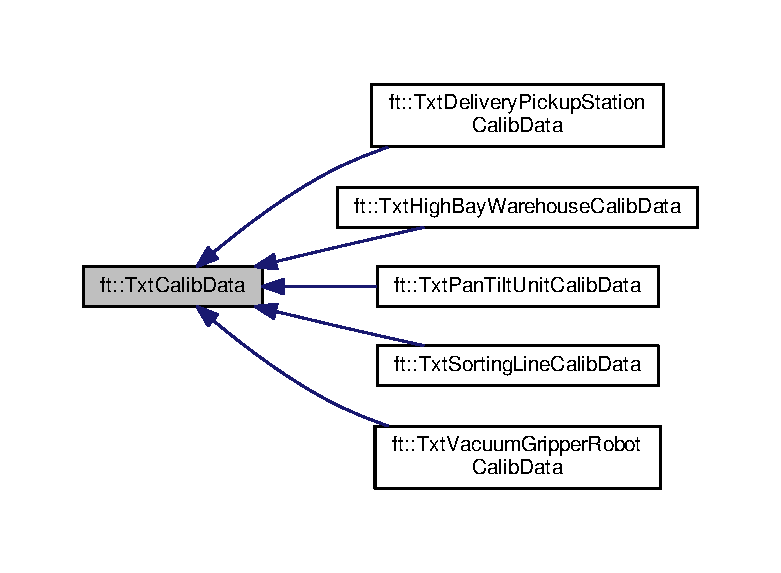
\includegraphics[width=350pt]{classft_1_1_txt_calib_data__inherit__graph}
\end{center}
\end{figure}
\subsection*{Public Member Functions}
\begin{DoxyCompactItemize}
\item 
\hyperlink{classft_1_1_txt_calib_data_a04d6b5689b2ef4973e5f4143e87bd24c}{Txt\+Calib\+Data} (std\+::string \hyperlink{classft_1_1_txt_calib_data_a4416924019587d7cb019b01652a20aab}{filename})
\item 
virtual \hyperlink{classft_1_1_txt_calib_data_ad3a67016c65d7c97ea7054d6997e3def}{$\sim$\+Txt\+Calib\+Data} ()
\item 
virtual bool \hyperlink{classft_1_1_txt_calib_data_abe888396c95ead8fd554fc77ba486e7a}{load} ()=0
\item 
virtual bool \hyperlink{classft_1_1_txt_calib_data_aace95b90ba43836acbd8f0cf1dd323c7}{save\+Default} ()=0
\item 
virtual bool \hyperlink{classft_1_1_txt_calib_data_a68a7bd5bfc32ebf82dd1a4fbe086a1b3}{save} ()=0
\item 
bool \hyperlink{classft_1_1_txt_calib_data_a85e3ba9c83b1143789c4116d946b476b}{is\+Valid} ()
\item 
bool \hyperlink{classft_1_1_txt_calib_data_aed66d1f47aaede36afe07185bef1eb9e}{exist\+Calib\+Filename} ()
\end{DoxyCompactItemize}
\subsection*{Protected Attributes}
\begin{DoxyCompactItemize}
\item 
std\+::string \hyperlink{classft_1_1_txt_calib_data_a4416924019587d7cb019b01652a20aab}{filename}
\item 
bool \hyperlink{classft_1_1_txt_calib_data_a0daecf43952003ea82b890dd266ae2c9}{valid}
\end{DoxyCompactItemize}


\subsection{Constructor \& Destructor Documentation}
\index{ft\+::\+Txt\+Calib\+Data@{ft\+::\+Txt\+Calib\+Data}!Txt\+Calib\+Data@{Txt\+Calib\+Data}}
\index{Txt\+Calib\+Data@{Txt\+Calib\+Data}!ft\+::\+Txt\+Calib\+Data@{ft\+::\+Txt\+Calib\+Data}}
\subsubsection[{\texorpdfstring{Txt\+Calib\+Data(std\+::string filename)}{TxtCalibData(std::string filename)}}]{\setlength{\rightskip}{0pt plus 5cm}ft\+::\+Txt\+Calib\+Data\+::\+Txt\+Calib\+Data (
\begin{DoxyParamCaption}
\item[{std\+::string}]{filename}
\end{DoxyParamCaption}
)}\hypertarget{classft_1_1_txt_calib_data_a04d6b5689b2ef4973e5f4143e87bd24c}{}\label{classft_1_1_txt_calib_data_a04d6b5689b2ef4973e5f4143e87bd24c}
\index{ft\+::\+Txt\+Calib\+Data@{ft\+::\+Txt\+Calib\+Data}!````~Txt\+Calib\+Data@{$\sim$\+Txt\+Calib\+Data}}
\index{````~Txt\+Calib\+Data@{$\sim$\+Txt\+Calib\+Data}!ft\+::\+Txt\+Calib\+Data@{ft\+::\+Txt\+Calib\+Data}}
\subsubsection[{\texorpdfstring{$\sim$\+Txt\+Calib\+Data()}{~TxtCalibData()}}]{\setlength{\rightskip}{0pt plus 5cm}virtual ft\+::\+Txt\+Calib\+Data\+::$\sim$\+Txt\+Calib\+Data (
\begin{DoxyParamCaption}
{}
\end{DoxyParamCaption}
)\hspace{0.3cm}{\ttfamily [virtual]}}\hypertarget{classft_1_1_txt_calib_data_ad3a67016c65d7c97ea7054d6997e3def}{}\label{classft_1_1_txt_calib_data_ad3a67016c65d7c97ea7054d6997e3def}


\subsection{Member Function Documentation}
\index{ft\+::\+Txt\+Calib\+Data@{ft\+::\+Txt\+Calib\+Data}!exist\+Calib\+Filename@{exist\+Calib\+Filename}}
\index{exist\+Calib\+Filename@{exist\+Calib\+Filename}!ft\+::\+Txt\+Calib\+Data@{ft\+::\+Txt\+Calib\+Data}}
\subsubsection[{\texorpdfstring{exist\+Calib\+Filename()}{existCalibFilename()}}]{\setlength{\rightskip}{0pt plus 5cm}bool ft\+::\+Txt\+Calib\+Data\+::exist\+Calib\+Filename (
\begin{DoxyParamCaption}
{}
\end{DoxyParamCaption}
)}\hypertarget{classft_1_1_txt_calib_data_aed66d1f47aaede36afe07185bef1eb9e}{}\label{classft_1_1_txt_calib_data_aed66d1f47aaede36afe07185bef1eb9e}
\index{ft\+::\+Txt\+Calib\+Data@{ft\+::\+Txt\+Calib\+Data}!is\+Valid@{is\+Valid}}
\index{is\+Valid@{is\+Valid}!ft\+::\+Txt\+Calib\+Data@{ft\+::\+Txt\+Calib\+Data}}
\subsubsection[{\texorpdfstring{is\+Valid()}{isValid()}}]{\setlength{\rightskip}{0pt plus 5cm}bool ft\+::\+Txt\+Calib\+Data\+::is\+Valid (
\begin{DoxyParamCaption}
{}
\end{DoxyParamCaption}
)\hspace{0.3cm}{\ttfamily [inline]}}\hypertarget{classft_1_1_txt_calib_data_a85e3ba9c83b1143789c4116d946b476b}{}\label{classft_1_1_txt_calib_data_a85e3ba9c83b1143789c4116d946b476b}
\index{ft\+::\+Txt\+Calib\+Data@{ft\+::\+Txt\+Calib\+Data}!load@{load}}
\index{load@{load}!ft\+::\+Txt\+Calib\+Data@{ft\+::\+Txt\+Calib\+Data}}
\subsubsection[{\texorpdfstring{load()=0}{load()=0}}]{\setlength{\rightskip}{0pt plus 5cm}virtual bool ft\+::\+Txt\+Calib\+Data\+::load (
\begin{DoxyParamCaption}
{}
\end{DoxyParamCaption}
)\hspace{0.3cm}{\ttfamily [pure virtual]}}\hypertarget{classft_1_1_txt_calib_data_abe888396c95ead8fd554fc77ba486e7a}{}\label{classft_1_1_txt_calib_data_abe888396c95ead8fd554fc77ba486e7a}


Implemented in \hyperlink{classft_1_1_txt_vacuum_gripper_robot_calib_data_a18a67b8766e89e205620d950b785afd4}{ft\+::\+Txt\+Vacuum\+Gripper\+Robot\+Calib\+Data}, \hyperlink{classft_1_1_txt_high_bay_warehouse_calib_data_a018f042864bebde45e9f138bff550ec9}{ft\+::\+Txt\+High\+Bay\+Warehouse\+Calib\+Data}, \hyperlink{classft_1_1_txt_pan_tilt_unit_calib_data_a0b609395ddd55b69596d8026a6a5bbb4}{ft\+::\+Txt\+Pan\+Tilt\+Unit\+Calib\+Data}, \hyperlink{classft_1_1_txt_sorting_line_calib_data_a2eb432107b17805eac5cae95604db8a5}{ft\+::\+Txt\+Sorting\+Line\+Calib\+Data}, and \hyperlink{classft_1_1_txt_delivery_pickup_station_calib_data_a6bb1679754a7cb50ef455a0b1241c08a}{ft\+::\+Txt\+Delivery\+Pickup\+Station\+Calib\+Data}.

\index{ft\+::\+Txt\+Calib\+Data@{ft\+::\+Txt\+Calib\+Data}!save@{save}}
\index{save@{save}!ft\+::\+Txt\+Calib\+Data@{ft\+::\+Txt\+Calib\+Data}}
\subsubsection[{\texorpdfstring{save()=0}{save()=0}}]{\setlength{\rightskip}{0pt plus 5cm}virtual bool ft\+::\+Txt\+Calib\+Data\+::save (
\begin{DoxyParamCaption}
{}
\end{DoxyParamCaption}
)\hspace{0.3cm}{\ttfamily [pure virtual]}}\hypertarget{classft_1_1_txt_calib_data_a68a7bd5bfc32ebf82dd1a4fbe086a1b3}{}\label{classft_1_1_txt_calib_data_a68a7bd5bfc32ebf82dd1a4fbe086a1b3}


Implemented in \hyperlink{classft_1_1_txt_vacuum_gripper_robot_calib_data_ae22aff2c5d480a15b6ea0b8f0ec71dc6}{ft\+::\+Txt\+Vacuum\+Gripper\+Robot\+Calib\+Data}, \hyperlink{classft_1_1_txt_high_bay_warehouse_calib_data_a193721ae3de0052eb1a3b74f877363a6}{ft\+::\+Txt\+High\+Bay\+Warehouse\+Calib\+Data}, \hyperlink{classft_1_1_txt_pan_tilt_unit_calib_data_a24f01720fce94850a038b68d5591895a}{ft\+::\+Txt\+Pan\+Tilt\+Unit\+Calib\+Data}, \hyperlink{classft_1_1_txt_sorting_line_calib_data_a14061e6b7938095185e5a07fda80101a}{ft\+::\+Txt\+Sorting\+Line\+Calib\+Data}, and \hyperlink{classft_1_1_txt_delivery_pickup_station_calib_data_a0d4f07c8ccbb254d8bc1d2b431790717}{ft\+::\+Txt\+Delivery\+Pickup\+Station\+Calib\+Data}.

\index{ft\+::\+Txt\+Calib\+Data@{ft\+::\+Txt\+Calib\+Data}!save\+Default@{save\+Default}}
\index{save\+Default@{save\+Default}!ft\+::\+Txt\+Calib\+Data@{ft\+::\+Txt\+Calib\+Data}}
\subsubsection[{\texorpdfstring{save\+Default()=0}{saveDefault()=0}}]{\setlength{\rightskip}{0pt plus 5cm}virtual bool ft\+::\+Txt\+Calib\+Data\+::save\+Default (
\begin{DoxyParamCaption}
{}
\end{DoxyParamCaption}
)\hspace{0.3cm}{\ttfamily [pure virtual]}}\hypertarget{classft_1_1_txt_calib_data_aace95b90ba43836acbd8f0cf1dd323c7}{}\label{classft_1_1_txt_calib_data_aace95b90ba43836acbd8f0cf1dd323c7}


Implemented in \hyperlink{classft_1_1_txt_vacuum_gripper_robot_calib_data_a620eb825a421524b94c78fb1f0db4a6c}{ft\+::\+Txt\+Vacuum\+Gripper\+Robot\+Calib\+Data}, \hyperlink{classft_1_1_txt_high_bay_warehouse_calib_data_ac8d87668f8d0347714f6545954df3573}{ft\+::\+Txt\+High\+Bay\+Warehouse\+Calib\+Data}, \hyperlink{classft_1_1_txt_pan_tilt_unit_calib_data_aa18d6ee3e2f9971e86baf69fa90d14cf}{ft\+::\+Txt\+Pan\+Tilt\+Unit\+Calib\+Data}, \hyperlink{classft_1_1_txt_sorting_line_calib_data_a98a160d82617960198b4b58da594d894}{ft\+::\+Txt\+Sorting\+Line\+Calib\+Data}, and \hyperlink{classft_1_1_txt_delivery_pickup_station_calib_data_a1cf9b3eb2a58d76ef84de23021c4e3bb}{ft\+::\+Txt\+Delivery\+Pickup\+Station\+Calib\+Data}.



\subsection{Member Data Documentation}
\index{ft\+::\+Txt\+Calib\+Data@{ft\+::\+Txt\+Calib\+Data}!filename@{filename}}
\index{filename@{filename}!ft\+::\+Txt\+Calib\+Data@{ft\+::\+Txt\+Calib\+Data}}
\subsubsection[{\texorpdfstring{filename}{filename}}]{\setlength{\rightskip}{0pt plus 5cm}std\+::string ft\+::\+Txt\+Calib\+Data\+::filename\hspace{0.3cm}{\ttfamily [protected]}}\hypertarget{classft_1_1_txt_calib_data_a4416924019587d7cb019b01652a20aab}{}\label{classft_1_1_txt_calib_data_a4416924019587d7cb019b01652a20aab}
\index{ft\+::\+Txt\+Calib\+Data@{ft\+::\+Txt\+Calib\+Data}!valid@{valid}}
\index{valid@{valid}!ft\+::\+Txt\+Calib\+Data@{ft\+::\+Txt\+Calib\+Data}}
\subsubsection[{\texorpdfstring{valid}{valid}}]{\setlength{\rightskip}{0pt plus 5cm}bool ft\+::\+Txt\+Calib\+Data\+::valid\hspace{0.3cm}{\ttfamily [protected]}}\hypertarget{classft_1_1_txt_calib_data_a0daecf43952003ea82b890dd266ae2c9}{}\label{classft_1_1_txt_calib_data_a0daecf43952003ea82b890dd266ae2c9}


The documentation for this class was generated from the following file\+:\begin{DoxyCompactItemize}
\item 
\hyperlink{_txt_calib_data_8h}{Txt\+Calib\+Data.\+h}\end{DoxyCompactItemize}

\hypertarget{classft_1_1_txt_camera}{}\section{ft\+:\+:Txt\+Camera Class Reference}
\label{classft_1_1_txt_camera}\index{ft\+::\+Txt\+Camera@{ft\+::\+Txt\+Camera}}


{\ttfamily \#include $<$Txt\+Camera.\+h$>$}



Inheritance diagram for ft\+:\+:Txt\+Camera\+:
\nopagebreak
\begin{figure}[H]
\begin{center}
\leavevmode
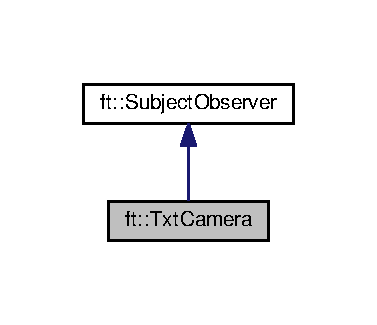
\includegraphics[width=181pt]{classft_1_1_txt_camera__inherit__graph}
\end{center}
\end{figure}


Collaboration diagram for ft\+:\+:Txt\+Camera\+:
\nopagebreak
\begin{figure}[H]
\begin{center}
\leavevmode
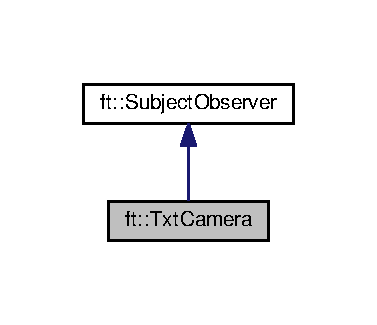
\includegraphics[width=181pt]{classft_1_1_txt_camera__coll__graph}
\end{center}
\end{figure}
\subsection*{Public Member Functions}
\begin{DoxyCompactItemize}
\item 
\hyperlink{classft_1_1_txt_camera_a4a32881e0772b23576c099ce651cf6c0}{Txt\+Camera} (double w=320, double h=240)
\item 
virtual \hyperlink{classft_1_1_txt_camera_a4e75e97e7a366c89c00d847011686a60}{$\sim$\+Txt\+Camera} ()
\item 
cv\+::\+Mat \hyperlink{classft_1_1_txt_camera_ad0ab6090018d8b9abfccba4c4e8e658e}{get\+Frame} ()
\item 
void \hyperlink{classft_1_1_txt_camera_a51ae2f7221426060932bd9896c6d64b4}{set\+Fps} (double f)
\item 
double \hyperlink{classft_1_1_txt_camera_aa2f94ecad8ee2d260160993b1a1d054f}{get\+Period} ()
\item 
bool \hyperlink{classft_1_1_txt_camera_ad03f2a8c15426da1c5d901bdafb79348}{start\+Thread} ()
\item 
bool \hyperlink{classft_1_1_txt_camera_ad8d5698a3eb2f63bfd59b18315ff9b87}{stop\+Thread} ()
\item 
void \hyperlink{classft_1_1_txt_camera_a958e24a713e1647f41d94efb8ffcef62}{start} ()
\item 
void \hyperlink{classft_1_1_txt_camera_a5a5d1ba7498d7933b1137b52d268c103}{stop} ()
\item 
bool \hyperlink{classft_1_1_txt_camera_a8f428838422813898c7cc216777ea60a}{read} ()
\item 
std\+::string \hyperlink{classft_1_1_txt_camera_aef7f03534d7a00d1cfec936bf5995f1f}{get\+Data\+String} ()
\item 
bool \hyperlink{classft_1_1_txt_camera_a2aee04f25709a3a9d40010190d1a2ba2}{write\+File} (const std\+::string \&filename)
\end{DoxyCompactItemize}
\subsection*{Protected Member Functions}
\begin{DoxyCompactItemize}
\item 
bool \hyperlink{classft_1_1_txt_camera_aba6fd06b03361b015a2ff6b59e7a9f72}{init} ()
\end{DoxyCompactItemize}


\subsection{Constructor \& Destructor Documentation}
\index{ft\+::\+Txt\+Camera@{ft\+::\+Txt\+Camera}!Txt\+Camera@{Txt\+Camera}}
\index{Txt\+Camera@{Txt\+Camera}!ft\+::\+Txt\+Camera@{ft\+::\+Txt\+Camera}}
\subsubsection[{\texorpdfstring{Txt\+Camera(double w=320, double h=240)}{TxtCamera(double w=320, double h=240)}}]{\setlength{\rightskip}{0pt plus 5cm}ft\+::\+Txt\+Camera\+::\+Txt\+Camera (
\begin{DoxyParamCaption}
\item[{double}]{w = {\ttfamily 320}, }
\item[{double}]{h = {\ttfamily 240}}
\end{DoxyParamCaption}
)}\hypertarget{classft_1_1_txt_camera_a4a32881e0772b23576c099ce651cf6c0}{}\label{classft_1_1_txt_camera_a4a32881e0772b23576c099ce651cf6c0}
\index{ft\+::\+Txt\+Camera@{ft\+::\+Txt\+Camera}!````~Txt\+Camera@{$\sim$\+Txt\+Camera}}
\index{````~Txt\+Camera@{$\sim$\+Txt\+Camera}!ft\+::\+Txt\+Camera@{ft\+::\+Txt\+Camera}}
\subsubsection[{\texorpdfstring{$\sim$\+Txt\+Camera()}{~TxtCamera()}}]{\setlength{\rightskip}{0pt plus 5cm}virtual ft\+::\+Txt\+Camera\+::$\sim$\+Txt\+Camera (
\begin{DoxyParamCaption}
{}
\end{DoxyParamCaption}
)\hspace{0.3cm}{\ttfamily [virtual]}}\hypertarget{classft_1_1_txt_camera_a4e75e97e7a366c89c00d847011686a60}{}\label{classft_1_1_txt_camera_a4e75e97e7a366c89c00d847011686a60}


\subsection{Member Function Documentation}
\index{ft\+::\+Txt\+Camera@{ft\+::\+Txt\+Camera}!get\+Data\+String@{get\+Data\+String}}
\index{get\+Data\+String@{get\+Data\+String}!ft\+::\+Txt\+Camera@{ft\+::\+Txt\+Camera}}
\subsubsection[{\texorpdfstring{get\+Data\+String()}{getDataString()}}]{\setlength{\rightskip}{0pt plus 5cm}std\+::string ft\+::\+Txt\+Camera\+::get\+Data\+String (
\begin{DoxyParamCaption}
{}
\end{DoxyParamCaption}
)}\hypertarget{classft_1_1_txt_camera_aef7f03534d7a00d1cfec936bf5995f1f}{}\label{classft_1_1_txt_camera_aef7f03534d7a00d1cfec936bf5995f1f}
\index{ft\+::\+Txt\+Camera@{ft\+::\+Txt\+Camera}!get\+Frame@{get\+Frame}}
\index{get\+Frame@{get\+Frame}!ft\+::\+Txt\+Camera@{ft\+::\+Txt\+Camera}}
\subsubsection[{\texorpdfstring{get\+Frame()}{getFrame()}}]{\setlength{\rightskip}{0pt plus 5cm}cv\+::\+Mat ft\+::\+Txt\+Camera\+::get\+Frame (
\begin{DoxyParamCaption}
{}
\end{DoxyParamCaption}
)}\hypertarget{classft_1_1_txt_camera_ad0ab6090018d8b9abfccba4c4e8e658e}{}\label{classft_1_1_txt_camera_ad0ab6090018d8b9abfccba4c4e8e658e}
\index{ft\+::\+Txt\+Camera@{ft\+::\+Txt\+Camera}!get\+Period@{get\+Period}}
\index{get\+Period@{get\+Period}!ft\+::\+Txt\+Camera@{ft\+::\+Txt\+Camera}}
\subsubsection[{\texorpdfstring{get\+Period()}{getPeriod()}}]{\setlength{\rightskip}{0pt plus 5cm}double ft\+::\+Txt\+Camera\+::get\+Period (
\begin{DoxyParamCaption}
{}
\end{DoxyParamCaption}
)\hspace{0.3cm}{\ttfamily [inline]}}\hypertarget{classft_1_1_txt_camera_aa2f94ecad8ee2d260160993b1a1d054f}{}\label{classft_1_1_txt_camera_aa2f94ecad8ee2d260160993b1a1d054f}
\index{ft\+::\+Txt\+Camera@{ft\+::\+Txt\+Camera}!init@{init}}
\index{init@{init}!ft\+::\+Txt\+Camera@{ft\+::\+Txt\+Camera}}
\subsubsection[{\texorpdfstring{init()}{init()}}]{\setlength{\rightskip}{0pt plus 5cm}bool ft\+::\+Txt\+Camera\+::init (
\begin{DoxyParamCaption}
{}
\end{DoxyParamCaption}
)\hspace{0.3cm}{\ttfamily [protected]}}\hypertarget{classft_1_1_txt_camera_aba6fd06b03361b015a2ff6b59e7a9f72}{}\label{classft_1_1_txt_camera_aba6fd06b03361b015a2ff6b59e7a9f72}
\index{ft\+::\+Txt\+Camera@{ft\+::\+Txt\+Camera}!read@{read}}
\index{read@{read}!ft\+::\+Txt\+Camera@{ft\+::\+Txt\+Camera}}
\subsubsection[{\texorpdfstring{read()}{read()}}]{\setlength{\rightskip}{0pt plus 5cm}bool ft\+::\+Txt\+Camera\+::read (
\begin{DoxyParamCaption}
{}
\end{DoxyParamCaption}
)}\hypertarget{classft_1_1_txt_camera_a8f428838422813898c7cc216777ea60a}{}\label{classft_1_1_txt_camera_a8f428838422813898c7cc216777ea60a}
\index{ft\+::\+Txt\+Camera@{ft\+::\+Txt\+Camera}!set\+Fps@{set\+Fps}}
\index{set\+Fps@{set\+Fps}!ft\+::\+Txt\+Camera@{ft\+::\+Txt\+Camera}}
\subsubsection[{\texorpdfstring{set\+Fps(double f)}{setFps(double f)}}]{\setlength{\rightskip}{0pt plus 5cm}void ft\+::\+Txt\+Camera\+::set\+Fps (
\begin{DoxyParamCaption}
\item[{double}]{f}
\end{DoxyParamCaption}
)\hspace{0.3cm}{\ttfamily [inline]}}\hypertarget{classft_1_1_txt_camera_a51ae2f7221426060932bd9896c6d64b4}{}\label{classft_1_1_txt_camera_a51ae2f7221426060932bd9896c6d64b4}
\index{ft\+::\+Txt\+Camera@{ft\+::\+Txt\+Camera}!start@{start}}
\index{start@{start}!ft\+::\+Txt\+Camera@{ft\+::\+Txt\+Camera}}
\subsubsection[{\texorpdfstring{start()}{start()}}]{\setlength{\rightskip}{0pt plus 5cm}void ft\+::\+Txt\+Camera\+::start (
\begin{DoxyParamCaption}
{}
\end{DoxyParamCaption}
)\hspace{0.3cm}{\ttfamily [inline]}}\hypertarget{classft_1_1_txt_camera_a958e24a713e1647f41d94efb8ffcef62}{}\label{classft_1_1_txt_camera_a958e24a713e1647f41d94efb8ffcef62}
\index{ft\+::\+Txt\+Camera@{ft\+::\+Txt\+Camera}!start\+Thread@{start\+Thread}}
\index{start\+Thread@{start\+Thread}!ft\+::\+Txt\+Camera@{ft\+::\+Txt\+Camera}}
\subsubsection[{\texorpdfstring{start\+Thread()}{startThread()}}]{\setlength{\rightskip}{0pt plus 5cm}bool ft\+::\+Txt\+Camera\+::start\+Thread (
\begin{DoxyParamCaption}
{}
\end{DoxyParamCaption}
)}\hypertarget{classft_1_1_txt_camera_ad03f2a8c15426da1c5d901bdafb79348}{}\label{classft_1_1_txt_camera_ad03f2a8c15426da1c5d901bdafb79348}
\index{ft\+::\+Txt\+Camera@{ft\+::\+Txt\+Camera}!stop@{stop}}
\index{stop@{stop}!ft\+::\+Txt\+Camera@{ft\+::\+Txt\+Camera}}
\subsubsection[{\texorpdfstring{stop()}{stop()}}]{\setlength{\rightskip}{0pt plus 5cm}void ft\+::\+Txt\+Camera\+::stop (
\begin{DoxyParamCaption}
{}
\end{DoxyParamCaption}
)\hspace{0.3cm}{\ttfamily [inline]}}\hypertarget{classft_1_1_txt_camera_a5a5d1ba7498d7933b1137b52d268c103}{}\label{classft_1_1_txt_camera_a5a5d1ba7498d7933b1137b52d268c103}
\index{ft\+::\+Txt\+Camera@{ft\+::\+Txt\+Camera}!stop\+Thread@{stop\+Thread}}
\index{stop\+Thread@{stop\+Thread}!ft\+::\+Txt\+Camera@{ft\+::\+Txt\+Camera}}
\subsubsection[{\texorpdfstring{stop\+Thread()}{stopThread()}}]{\setlength{\rightskip}{0pt plus 5cm}bool ft\+::\+Txt\+Camera\+::stop\+Thread (
\begin{DoxyParamCaption}
{}
\end{DoxyParamCaption}
)}\hypertarget{classft_1_1_txt_camera_ad8d5698a3eb2f63bfd59b18315ff9b87}{}\label{classft_1_1_txt_camera_ad8d5698a3eb2f63bfd59b18315ff9b87}
\index{ft\+::\+Txt\+Camera@{ft\+::\+Txt\+Camera}!write\+File@{write\+File}}
\index{write\+File@{write\+File}!ft\+::\+Txt\+Camera@{ft\+::\+Txt\+Camera}}
\subsubsection[{\texorpdfstring{write\+File(const std\+::string \&filename)}{writeFile(const std::string &filename)}}]{\setlength{\rightskip}{0pt plus 5cm}bool ft\+::\+Txt\+Camera\+::write\+File (
\begin{DoxyParamCaption}
\item[{const std\+::string \&}]{filename}
\end{DoxyParamCaption}
)}\hypertarget{classft_1_1_txt_camera_a2aee04f25709a3a9d40010190d1a2ba2}{}\label{classft_1_1_txt_camera_a2aee04f25709a3a9d40010190d1a2ba2}


The documentation for this class was generated from the following file\+:\begin{DoxyCompactItemize}
\item 
\hyperlink{_txt_camera_8h}{Txt\+Camera.\+h}\end{DoxyCompactItemize}

\hypertarget{classft_1_1_txt_conveyor_belt}{}\section{ft\+:\+:Txt\+Conveyor\+Belt Class Reference}
\label{classft_1_1_txt_conveyor_belt}\index{ft\+::\+Txt\+Conveyor\+Belt@{ft\+::\+Txt\+Conveyor\+Belt}}


{\ttfamily \#include $<$Txt\+Conveyor\+Belt.\+h$>$}



Inheritance diagram for ft\+:\+:Txt\+Conveyor\+Belt\+:
\nopagebreak
\begin{figure}[H]
\begin{center}
\leavevmode
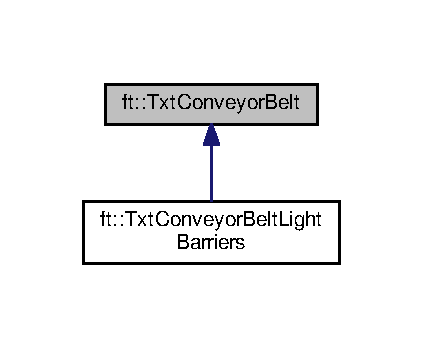
\includegraphics[width=203pt]{classft_1_1_txt_conveyor_belt__inherit__graph}
\end{center}
\end{figure}
\subsection*{Public Member Functions}
\begin{DoxyCompactItemize}
\item 
\hyperlink{classft_1_1_txt_conveyor_belt_aa0c6d359db7e29ef06f2d1f7aede6347}{Txt\+Conveyor\+Belt} (F\+I\+S\+H\+\_\+\+X1\+\_\+\+T\+R\+A\+N\+S\+F\+ER $\ast$\hyperlink{classft_1_1_txt_conveyor_belt_aee7d4f810563d6e97a64aaa8bf0dcce0}{p\+T\+Area}, uint8\+\_\+t \hyperlink{classft_1_1_txt_conveyor_belt_a25369fe466fdbe778e9ffa25c0ae6d0f}{chM})
\item 
virtual \hyperlink{classft_1_1_txt_conveyor_belt_ab1d5269a7deaf5aa0533e543fb668e76}{$\sim$\+Txt\+Conveyor\+Belt} ()
\item 
void \hyperlink{classft_1_1_txt_conveyor_belt_abb63916dcdc8a7c6134271e478103394}{set\+Speed} (int16\+\_\+t s)
\item 
int16\+\_\+t \hyperlink{classft_1_1_txt_conveyor_belt_a9afad7b1fcadd2f97886df29e232d2b1}{get\+Speed} ()
\item 
void \hyperlink{classft_1_1_txt_conveyor_belt_a0dbd0de0d73bbc16711b46985ecd5744}{move\+Left} ()
\item 
void \hyperlink{classft_1_1_txt_conveyor_belt_a55944a69d517ca45240e8561bf79d422}{move\+Right} ()
\item 
void \hyperlink{classft_1_1_txt_conveyor_belt_a645b5ecc1e6e7a7efb5ee281ca252aa5}{stop} ()
\end{DoxyCompactItemize}
\subsection*{Protected Attributes}
\begin{DoxyCompactItemize}
\item 
F\+I\+S\+H\+\_\+\+X1\+\_\+\+T\+R\+A\+N\+S\+F\+ER $\ast$ \hyperlink{classft_1_1_txt_conveyor_belt_aee7d4f810563d6e97a64aaa8bf0dcce0}{p\+T\+Area}
\item 
uint8\+\_\+t \hyperlink{classft_1_1_txt_conveyor_belt_a25369fe466fdbe778e9ffa25c0ae6d0f}{chM}
\item 
int16\+\_\+t \hyperlink{classft_1_1_txt_conveyor_belt_ac5f6a0524423c76eead496610584782d}{speed}
\end{DoxyCompactItemize}


\subsection{Constructor \& Destructor Documentation}
\index{ft\+::\+Txt\+Conveyor\+Belt@{ft\+::\+Txt\+Conveyor\+Belt}!Txt\+Conveyor\+Belt@{Txt\+Conveyor\+Belt}}
\index{Txt\+Conveyor\+Belt@{Txt\+Conveyor\+Belt}!ft\+::\+Txt\+Conveyor\+Belt@{ft\+::\+Txt\+Conveyor\+Belt}}
\subsubsection[{\texorpdfstring{Txt\+Conveyor\+Belt(\+F\+I\+S\+H\+\_\+\+X1\+\_\+\+T\+R\+A\+N\+S\+F\+E\+R $\ast$p\+T\+Area, uint8\+\_\+t ch\+M)}{TxtConveyorBelt(FISH_X1_TRANSFER *pTArea, uint8_t chM)}}]{\setlength{\rightskip}{0pt plus 5cm}ft\+::\+Txt\+Conveyor\+Belt\+::\+Txt\+Conveyor\+Belt (
\begin{DoxyParamCaption}
\item[{F\+I\+S\+H\+\_\+\+X1\+\_\+\+T\+R\+A\+N\+S\+F\+ER $\ast$}]{p\+T\+Area, }
\item[{uint8\+\_\+t}]{chM}
\end{DoxyParamCaption}
)}\hypertarget{classft_1_1_txt_conveyor_belt_aa0c6d359db7e29ef06f2d1f7aede6347}{}\label{classft_1_1_txt_conveyor_belt_aa0c6d359db7e29ef06f2d1f7aede6347}
\index{ft\+::\+Txt\+Conveyor\+Belt@{ft\+::\+Txt\+Conveyor\+Belt}!````~Txt\+Conveyor\+Belt@{$\sim$\+Txt\+Conveyor\+Belt}}
\index{````~Txt\+Conveyor\+Belt@{$\sim$\+Txt\+Conveyor\+Belt}!ft\+::\+Txt\+Conveyor\+Belt@{ft\+::\+Txt\+Conveyor\+Belt}}
\subsubsection[{\texorpdfstring{$\sim$\+Txt\+Conveyor\+Belt()}{~TxtConveyorBelt()}}]{\setlength{\rightskip}{0pt plus 5cm}virtual ft\+::\+Txt\+Conveyor\+Belt\+::$\sim$\+Txt\+Conveyor\+Belt (
\begin{DoxyParamCaption}
{}
\end{DoxyParamCaption}
)\hspace{0.3cm}{\ttfamily [virtual]}}\hypertarget{classft_1_1_txt_conveyor_belt_ab1d5269a7deaf5aa0533e543fb668e76}{}\label{classft_1_1_txt_conveyor_belt_ab1d5269a7deaf5aa0533e543fb668e76}


\subsection{Member Function Documentation}
\index{ft\+::\+Txt\+Conveyor\+Belt@{ft\+::\+Txt\+Conveyor\+Belt}!get\+Speed@{get\+Speed}}
\index{get\+Speed@{get\+Speed}!ft\+::\+Txt\+Conveyor\+Belt@{ft\+::\+Txt\+Conveyor\+Belt}}
\subsubsection[{\texorpdfstring{get\+Speed()}{getSpeed()}}]{\setlength{\rightskip}{0pt plus 5cm}int16\+\_\+t ft\+::\+Txt\+Conveyor\+Belt\+::get\+Speed (
\begin{DoxyParamCaption}
{}
\end{DoxyParamCaption}
)\hspace{0.3cm}{\ttfamily [inline]}}\hypertarget{classft_1_1_txt_conveyor_belt_a9afad7b1fcadd2f97886df29e232d2b1}{}\label{classft_1_1_txt_conveyor_belt_a9afad7b1fcadd2f97886df29e232d2b1}
\index{ft\+::\+Txt\+Conveyor\+Belt@{ft\+::\+Txt\+Conveyor\+Belt}!move\+Left@{move\+Left}}
\index{move\+Left@{move\+Left}!ft\+::\+Txt\+Conveyor\+Belt@{ft\+::\+Txt\+Conveyor\+Belt}}
\subsubsection[{\texorpdfstring{move\+Left()}{moveLeft()}}]{\setlength{\rightskip}{0pt plus 5cm}void ft\+::\+Txt\+Conveyor\+Belt\+::move\+Left (
\begin{DoxyParamCaption}
{}
\end{DoxyParamCaption}
)}\hypertarget{classft_1_1_txt_conveyor_belt_a0dbd0de0d73bbc16711b46985ecd5744}{}\label{classft_1_1_txt_conveyor_belt_a0dbd0de0d73bbc16711b46985ecd5744}
\index{ft\+::\+Txt\+Conveyor\+Belt@{ft\+::\+Txt\+Conveyor\+Belt}!move\+Right@{move\+Right}}
\index{move\+Right@{move\+Right}!ft\+::\+Txt\+Conveyor\+Belt@{ft\+::\+Txt\+Conveyor\+Belt}}
\subsubsection[{\texorpdfstring{move\+Right()}{moveRight()}}]{\setlength{\rightskip}{0pt plus 5cm}void ft\+::\+Txt\+Conveyor\+Belt\+::move\+Right (
\begin{DoxyParamCaption}
{}
\end{DoxyParamCaption}
)}\hypertarget{classft_1_1_txt_conveyor_belt_a55944a69d517ca45240e8561bf79d422}{}\label{classft_1_1_txt_conveyor_belt_a55944a69d517ca45240e8561bf79d422}
\index{ft\+::\+Txt\+Conveyor\+Belt@{ft\+::\+Txt\+Conveyor\+Belt}!set\+Speed@{set\+Speed}}
\index{set\+Speed@{set\+Speed}!ft\+::\+Txt\+Conveyor\+Belt@{ft\+::\+Txt\+Conveyor\+Belt}}
\subsubsection[{\texorpdfstring{set\+Speed(int16\+\_\+t s)}{setSpeed(int16_t s)}}]{\setlength{\rightskip}{0pt plus 5cm}void ft\+::\+Txt\+Conveyor\+Belt\+::set\+Speed (
\begin{DoxyParamCaption}
\item[{int16\+\_\+t}]{s}
\end{DoxyParamCaption}
)}\hypertarget{classft_1_1_txt_conveyor_belt_abb63916dcdc8a7c6134271e478103394}{}\label{classft_1_1_txt_conveyor_belt_abb63916dcdc8a7c6134271e478103394}
\index{ft\+::\+Txt\+Conveyor\+Belt@{ft\+::\+Txt\+Conveyor\+Belt}!stop@{stop}}
\index{stop@{stop}!ft\+::\+Txt\+Conveyor\+Belt@{ft\+::\+Txt\+Conveyor\+Belt}}
\subsubsection[{\texorpdfstring{stop()}{stop()}}]{\setlength{\rightskip}{0pt plus 5cm}void ft\+::\+Txt\+Conveyor\+Belt\+::stop (
\begin{DoxyParamCaption}
{}
\end{DoxyParamCaption}
)}\hypertarget{classft_1_1_txt_conveyor_belt_a645b5ecc1e6e7a7efb5ee281ca252aa5}{}\label{classft_1_1_txt_conveyor_belt_a645b5ecc1e6e7a7efb5ee281ca252aa5}


\subsection{Member Data Documentation}
\index{ft\+::\+Txt\+Conveyor\+Belt@{ft\+::\+Txt\+Conveyor\+Belt}!chM@{chM}}
\index{chM@{chM}!ft\+::\+Txt\+Conveyor\+Belt@{ft\+::\+Txt\+Conveyor\+Belt}}
\subsubsection[{\texorpdfstring{chM}{chM}}]{\setlength{\rightskip}{0pt plus 5cm}uint8\+\_\+t ft\+::\+Txt\+Conveyor\+Belt\+::chM\hspace{0.3cm}{\ttfamily [protected]}}\hypertarget{classft_1_1_txt_conveyor_belt_a25369fe466fdbe778e9ffa25c0ae6d0f}{}\label{classft_1_1_txt_conveyor_belt_a25369fe466fdbe778e9ffa25c0ae6d0f}
\index{ft\+::\+Txt\+Conveyor\+Belt@{ft\+::\+Txt\+Conveyor\+Belt}!p\+T\+Area@{p\+T\+Area}}
\index{p\+T\+Area@{p\+T\+Area}!ft\+::\+Txt\+Conveyor\+Belt@{ft\+::\+Txt\+Conveyor\+Belt}}
\subsubsection[{\texorpdfstring{p\+T\+Area}{pTArea}}]{\setlength{\rightskip}{0pt plus 5cm}F\+I\+S\+H\+\_\+\+X1\+\_\+\+T\+R\+A\+N\+S\+F\+ER$\ast$ ft\+::\+Txt\+Conveyor\+Belt\+::p\+T\+Area\hspace{0.3cm}{\ttfamily [protected]}}\hypertarget{classft_1_1_txt_conveyor_belt_aee7d4f810563d6e97a64aaa8bf0dcce0}{}\label{classft_1_1_txt_conveyor_belt_aee7d4f810563d6e97a64aaa8bf0dcce0}
\index{ft\+::\+Txt\+Conveyor\+Belt@{ft\+::\+Txt\+Conveyor\+Belt}!speed@{speed}}
\index{speed@{speed}!ft\+::\+Txt\+Conveyor\+Belt@{ft\+::\+Txt\+Conveyor\+Belt}}
\subsubsection[{\texorpdfstring{speed}{speed}}]{\setlength{\rightskip}{0pt plus 5cm}int16\+\_\+t ft\+::\+Txt\+Conveyor\+Belt\+::speed\hspace{0.3cm}{\ttfamily [protected]}}\hypertarget{classft_1_1_txt_conveyor_belt_ac5f6a0524423c76eead496610584782d}{}\label{classft_1_1_txt_conveyor_belt_ac5f6a0524423c76eead496610584782d}


The documentation for this class was generated from the following file\+:\begin{DoxyCompactItemize}
\item 
\hyperlink{_txt_conveyor_belt_8h}{Txt\+Conveyor\+Belt.\+h}\end{DoxyCompactItemize}

\hypertarget{classft_1_1_txt_conveyor_belt_light_barriers}{}\section{ft\+:\+:Txt\+Conveyor\+Belt\+Light\+Barriers Class Reference}
\label{classft_1_1_txt_conveyor_belt_light_barriers}\index{ft\+::\+Txt\+Conveyor\+Belt\+Light\+Barriers@{ft\+::\+Txt\+Conveyor\+Belt\+Light\+Barriers}}


{\ttfamily \#include $<$Txt\+Conveyor\+Belt.\+h$>$}



Inheritance diagram for ft\+:\+:Txt\+Conveyor\+Belt\+Light\+Barriers\+:
\nopagebreak
\begin{figure}[H]
\begin{center}
\leavevmode
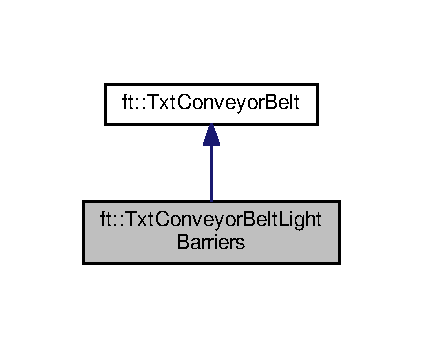
\includegraphics[width=203pt]{classft_1_1_txt_conveyor_belt_light_barriers__inherit__graph}
\end{center}
\end{figure}


Collaboration diagram for ft\+:\+:Txt\+Conveyor\+Belt\+Light\+Barriers\+:
\nopagebreak
\begin{figure}[H]
\begin{center}
\leavevmode
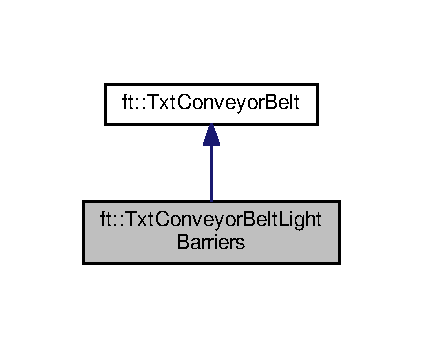
\includegraphics[width=203pt]{classft_1_1_txt_conveyor_belt_light_barriers__coll__graph}
\end{center}
\end{figure}
\subsection*{Public Member Functions}
\begin{DoxyCompactItemize}
\item 
\hyperlink{classft_1_1_txt_conveyor_belt_light_barriers_a9427ae97ee7a54ecf60e405b800c8e70}{Txt\+Conveyor\+Belt\+Light\+Barriers} (F\+I\+S\+H\+\_\+\+X1\+\_\+\+T\+R\+A\+N\+S\+F\+ER $\ast$\hyperlink{classft_1_1_txt_conveyor_belt_aee7d4f810563d6e97a64aaa8bf0dcce0}{p\+T\+Area}, uint8\+\_\+t \hyperlink{classft_1_1_txt_conveyor_belt_a25369fe466fdbe778e9ffa25c0ae6d0f}{chM}, int \hyperlink{classft_1_1_txt_conveyor_belt_light_barriers_ae2d3931fccc38e20402a3b3aad4c1baa}{ch\+L1}, int \hyperlink{classft_1_1_txt_conveyor_belt_light_barriers_af9383c0faa8024f9b50d38dd9938a6ac}{ch\+L2})
\item 
virtual \hyperlink{classft_1_1_txt_conveyor_belt_light_barriers_aa6d6acb063ced5ef20b7901e88c13291}{$\sim$\+Txt\+Conveyor\+Belt\+Light\+Barriers} ()
\item 
void \hyperlink{classft_1_1_txt_conveyor_belt_light_barriers_af3a95dfd86db23bf00abce758e81d1ba}{move\+In} ()
\item 
void \hyperlink{classft_1_1_txt_conveyor_belt_light_barriers_ac8ba406e1508f34b496ce7115e24f314}{move\+Out} ()
\end{DoxyCompactItemize}
\subsection*{Protected Attributes}
\begin{DoxyCompactItemize}
\item 
uint8\+\_\+t \hyperlink{classft_1_1_txt_conveyor_belt_light_barriers_ae2d3931fccc38e20402a3b3aad4c1baa}{ch\+L1}
\item 
uint8\+\_\+t \hyperlink{classft_1_1_txt_conveyor_belt_light_barriers_af9383c0faa8024f9b50d38dd9938a6ac}{ch\+L2}
\end{DoxyCompactItemize}


\subsection{Constructor \& Destructor Documentation}
\index{ft\+::\+Txt\+Conveyor\+Belt\+Light\+Barriers@{ft\+::\+Txt\+Conveyor\+Belt\+Light\+Barriers}!Txt\+Conveyor\+Belt\+Light\+Barriers@{Txt\+Conveyor\+Belt\+Light\+Barriers}}
\index{Txt\+Conveyor\+Belt\+Light\+Barriers@{Txt\+Conveyor\+Belt\+Light\+Barriers}!ft\+::\+Txt\+Conveyor\+Belt\+Light\+Barriers@{ft\+::\+Txt\+Conveyor\+Belt\+Light\+Barriers}}
\subsubsection[{\texorpdfstring{Txt\+Conveyor\+Belt\+Light\+Barriers(\+F\+I\+S\+H\+\_\+\+X1\+\_\+\+T\+R\+A\+N\+S\+F\+E\+R $\ast$p\+T\+Area, uint8\+\_\+t ch\+M, int ch\+L1, int ch\+L2)}{TxtConveyorBeltLightBarriers(FISH_X1_TRANSFER *pTArea, uint8_t chM, int chL1, int chL2)}}]{\setlength{\rightskip}{0pt plus 5cm}ft\+::\+Txt\+Conveyor\+Belt\+Light\+Barriers\+::\+Txt\+Conveyor\+Belt\+Light\+Barriers (
\begin{DoxyParamCaption}
\item[{F\+I\+S\+H\+\_\+\+X1\+\_\+\+T\+R\+A\+N\+S\+F\+ER $\ast$}]{p\+T\+Area, }
\item[{uint8\+\_\+t}]{chM, }
\item[{int}]{ch\+L1, }
\item[{int}]{ch\+L2}
\end{DoxyParamCaption}
)}\hypertarget{classft_1_1_txt_conveyor_belt_light_barriers_a9427ae97ee7a54ecf60e405b800c8e70}{}\label{classft_1_1_txt_conveyor_belt_light_barriers_a9427ae97ee7a54ecf60e405b800c8e70}
\index{ft\+::\+Txt\+Conveyor\+Belt\+Light\+Barriers@{ft\+::\+Txt\+Conveyor\+Belt\+Light\+Barriers}!````~Txt\+Conveyor\+Belt\+Light\+Barriers@{$\sim$\+Txt\+Conveyor\+Belt\+Light\+Barriers}}
\index{````~Txt\+Conveyor\+Belt\+Light\+Barriers@{$\sim$\+Txt\+Conveyor\+Belt\+Light\+Barriers}!ft\+::\+Txt\+Conveyor\+Belt\+Light\+Barriers@{ft\+::\+Txt\+Conveyor\+Belt\+Light\+Barriers}}
\subsubsection[{\texorpdfstring{$\sim$\+Txt\+Conveyor\+Belt\+Light\+Barriers()}{~TxtConveyorBeltLightBarriers()}}]{\setlength{\rightskip}{0pt plus 5cm}virtual ft\+::\+Txt\+Conveyor\+Belt\+Light\+Barriers\+::$\sim$\+Txt\+Conveyor\+Belt\+Light\+Barriers (
\begin{DoxyParamCaption}
{}
\end{DoxyParamCaption}
)\hspace{0.3cm}{\ttfamily [virtual]}}\hypertarget{classft_1_1_txt_conveyor_belt_light_barriers_aa6d6acb063ced5ef20b7901e88c13291}{}\label{classft_1_1_txt_conveyor_belt_light_barriers_aa6d6acb063ced5ef20b7901e88c13291}


\subsection{Member Function Documentation}
\index{ft\+::\+Txt\+Conveyor\+Belt\+Light\+Barriers@{ft\+::\+Txt\+Conveyor\+Belt\+Light\+Barriers}!move\+In@{move\+In}}
\index{move\+In@{move\+In}!ft\+::\+Txt\+Conveyor\+Belt\+Light\+Barriers@{ft\+::\+Txt\+Conveyor\+Belt\+Light\+Barriers}}
\subsubsection[{\texorpdfstring{move\+In()}{moveIn()}}]{\setlength{\rightskip}{0pt plus 5cm}void ft\+::\+Txt\+Conveyor\+Belt\+Light\+Barriers\+::move\+In (
\begin{DoxyParamCaption}
{}
\end{DoxyParamCaption}
)}\hypertarget{classft_1_1_txt_conveyor_belt_light_barriers_af3a95dfd86db23bf00abce758e81d1ba}{}\label{classft_1_1_txt_conveyor_belt_light_barriers_af3a95dfd86db23bf00abce758e81d1ba}
\index{ft\+::\+Txt\+Conveyor\+Belt\+Light\+Barriers@{ft\+::\+Txt\+Conveyor\+Belt\+Light\+Barriers}!move\+Out@{move\+Out}}
\index{move\+Out@{move\+Out}!ft\+::\+Txt\+Conveyor\+Belt\+Light\+Barriers@{ft\+::\+Txt\+Conveyor\+Belt\+Light\+Barriers}}
\subsubsection[{\texorpdfstring{move\+Out()}{moveOut()}}]{\setlength{\rightskip}{0pt plus 5cm}void ft\+::\+Txt\+Conveyor\+Belt\+Light\+Barriers\+::move\+Out (
\begin{DoxyParamCaption}
{}
\end{DoxyParamCaption}
)}\hypertarget{classft_1_1_txt_conveyor_belt_light_barriers_ac8ba406e1508f34b496ce7115e24f314}{}\label{classft_1_1_txt_conveyor_belt_light_barriers_ac8ba406e1508f34b496ce7115e24f314}


\subsection{Member Data Documentation}
\index{ft\+::\+Txt\+Conveyor\+Belt\+Light\+Barriers@{ft\+::\+Txt\+Conveyor\+Belt\+Light\+Barriers}!ch\+L1@{ch\+L1}}
\index{ch\+L1@{ch\+L1}!ft\+::\+Txt\+Conveyor\+Belt\+Light\+Barriers@{ft\+::\+Txt\+Conveyor\+Belt\+Light\+Barriers}}
\subsubsection[{\texorpdfstring{ch\+L1}{chL1}}]{\setlength{\rightskip}{0pt plus 5cm}uint8\+\_\+t ft\+::\+Txt\+Conveyor\+Belt\+Light\+Barriers\+::ch\+L1\hspace{0.3cm}{\ttfamily [protected]}}\hypertarget{classft_1_1_txt_conveyor_belt_light_barriers_ae2d3931fccc38e20402a3b3aad4c1baa}{}\label{classft_1_1_txt_conveyor_belt_light_barriers_ae2d3931fccc38e20402a3b3aad4c1baa}
\index{ft\+::\+Txt\+Conveyor\+Belt\+Light\+Barriers@{ft\+::\+Txt\+Conveyor\+Belt\+Light\+Barriers}!ch\+L2@{ch\+L2}}
\index{ch\+L2@{ch\+L2}!ft\+::\+Txt\+Conveyor\+Belt\+Light\+Barriers@{ft\+::\+Txt\+Conveyor\+Belt\+Light\+Barriers}}
\subsubsection[{\texorpdfstring{ch\+L2}{chL2}}]{\setlength{\rightskip}{0pt plus 5cm}uint8\+\_\+t ft\+::\+Txt\+Conveyor\+Belt\+Light\+Barriers\+::ch\+L2\hspace{0.3cm}{\ttfamily [protected]}}\hypertarget{classft_1_1_txt_conveyor_belt_light_barriers_af9383c0faa8024f9b50d38dd9938a6ac}{}\label{classft_1_1_txt_conveyor_belt_light_barriers_af9383c0faa8024f9b50d38dd9938a6ac}


The documentation for this class was generated from the following file\+:\begin{DoxyCompactItemize}
\item 
\hyperlink{_txt_conveyor_belt_8h}{Txt\+Conveyor\+Belt.\+h}\end{DoxyCompactItemize}

\hypertarget{classft_1_1_txt_delivery_pickup_station}{}\section{ft\+:\+:Txt\+Delivery\+Pickup\+Station Class Reference}
\label{classft_1_1_txt_delivery_pickup_station}\index{ft\+::\+Txt\+Delivery\+Pickup\+Station@{ft\+::\+Txt\+Delivery\+Pickup\+Station}}


{\ttfamily \#include $<$Txt\+Delivery\+Pickup\+Station.\+h$>$}



Inheritance diagram for ft\+:\+:Txt\+Delivery\+Pickup\+Station\+:
\nopagebreak
\begin{figure}[H]
\begin{center}
\leavevmode
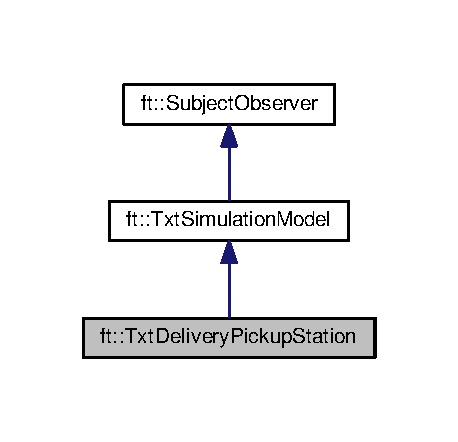
\includegraphics[width=220pt]{classft_1_1_txt_delivery_pickup_station__inherit__graph}
\end{center}
\end{figure}


Collaboration diagram for ft\+:\+:Txt\+Delivery\+Pickup\+Station\+:
\nopagebreak
\begin{figure}[H]
\begin{center}
\leavevmode
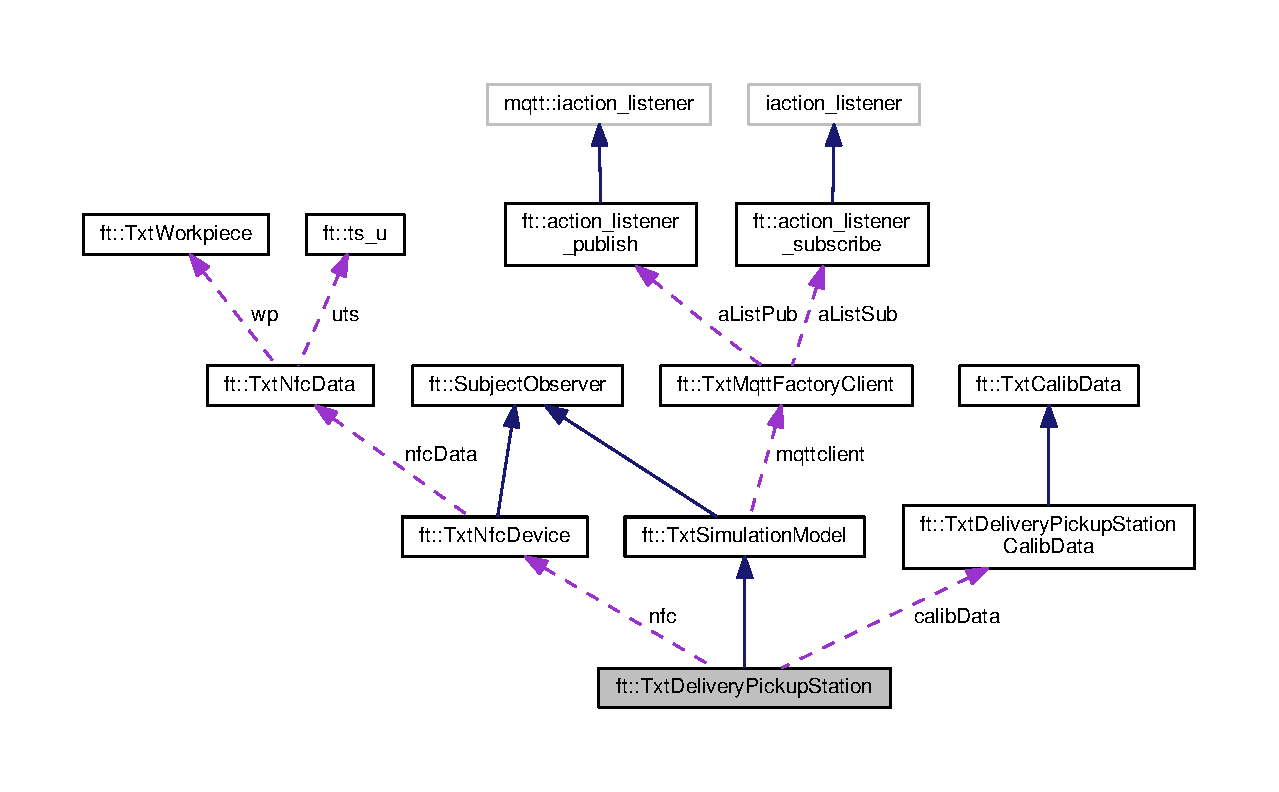
\includegraphics[width=350pt]{classft_1_1_txt_delivery_pickup_station__coll__graph}
\end{center}
\end{figure}
\subsection*{Public Member Functions}
\begin{DoxyCompactItemize}
\item 
\hyperlink{classft_1_1_txt_delivery_pickup_station_acafb3a6e67a1dc10f4cbf8c21629bf0f}{Txt\+Delivery\+Pickup\+Station} (F\+I\+S\+H\+\_\+\+X1\+\_\+\+T\+R\+A\+N\+S\+F\+ER $\ast$\hyperlink{classft_1_1_txt_simulation_model_a9facd66a0dbecd676ae7b72c37a0b300}{p\+T\+Area}, \hyperlink{classft_1_1_txt_mqtt_factory_client}{ft\+::\+Txt\+Mqtt\+Factory\+Client} $\ast$\hyperlink{classft_1_1_txt_simulation_model_a6a92fdef8619b9b1636c7c464091ea3a}{mqttclient})
\item 
virtual \hyperlink{classft_1_1_txt_delivery_pickup_station_aa6a9fd39473743f7b1f61e46bceed3ab}{$\sim$\+Txt\+Delivery\+Pickup\+Station} ()
\item 
std\+::string \hyperlink{classft_1_1_txt_delivery_pickup_station_af67559e392ce22b20e52b36f9f0ddc16}{nfc\+Device\+Delete\+Write\+Raw\+Read} (std\+::vector$<$ int64\+\_\+t $>$ vts, uint8\+\_\+t mask\+\_\+ts)
\item 
std\+::string \hyperlink{classft_1_1_txt_delivery_pickup_station_a78b7b2f725fff8c83298a9b0c17c8001}{nfc\+Device\+Write\+Produced\+Read} (std\+::vector$<$ int64\+\_\+t $>$ vts, uint8\+\_\+t mask\+\_\+ts)
\item 
std\+::string \hyperlink{classft_1_1_txt_delivery_pickup_station_a3a1868466d61182623dfa86ffe747539}{nfc\+Device\+Write\+Rejected\+Read} (std\+::vector$<$ int64\+\_\+t $>$ vts, uint8\+\_\+t mask\+\_\+ts)
\item 
bool \hyperlink{classft_1_1_txt_delivery_pickup_station_a2379511e7da862e4ae0ec0b2aa568d05}{is\+\_\+\+D\+IN} ()
\item 
bool \hyperlink{classft_1_1_txt_delivery_pickup_station_a1b2ec468c94caef59ab92171cd5420b0}{is\+\_\+\+D\+O\+UT} ()
\item 
std\+::string \hyperlink{classft_1_1_txt_delivery_pickup_station_abc2dad3c5b2013af93f113bb90230797}{get\+U\+I\+D\+Calib\+Mode} ()
\item 
std\+::string \hyperlink{classft_1_1_txt_delivery_pickup_station_a59e7d70b08cd4c5e84e21bfa22d010af}{get\+U\+I\+D\+Reset\+H\+BW} ()
\item 
std\+::string \hyperlink{classft_1_1_txt_delivery_pickup_station_a7bf2dc1487892e8f66f2fa2b1f3d4711}{get\+U\+I\+D\+Order\+W\+H\+I\+TE} ()
\item 
std\+::string \hyperlink{classft_1_1_txt_delivery_pickup_station_a6cf61e92c3ca2a0714aab0c10e20bc0d}{get\+U\+I\+D\+Order\+R\+ED} ()
\item 
std\+::string \hyperlink{classft_1_1_txt_delivery_pickup_station_acae940a2dd3ddb7574de62f8acda3efe}{get\+U\+I\+D\+Order\+B\+L\+UE} ()
\item 
void \hyperlink{classft_1_1_txt_delivery_pickup_station_ab53d853ce517143fc7f366c35c9c9320}{save\+U\+I\+D\+Calib\+Mode} (std\+::string uid)
\item 
void \hyperlink{classft_1_1_txt_delivery_pickup_station_a97f61e85f04760e73b8dfeb5c0dda06d}{save\+U\+I\+D\+Reset\+H\+BW} (std\+::string uid)
\item 
void \hyperlink{classft_1_1_txt_delivery_pickup_station_a512e9257c9e08dedd3cc6fab50b5184d}{save\+U\+I\+D\+Order\+W\+H\+I\+TE} (std\+::string uid)
\item 
void \hyperlink{classft_1_1_txt_delivery_pickup_station_aa0f590a1934992f560c10af54d21cf3a}{save\+U\+I\+D\+Order\+R\+ED} (std\+::string uid)
\item 
void \hyperlink{classft_1_1_txt_delivery_pickup_station_af92b3ea609de2523942e56564f976262}{save\+U\+I\+D\+Order\+B\+L\+UE} (std\+::string uid)
\item 
int \hyperlink{classft_1_1_txt_delivery_pickup_station_af105371e606d2156bc78ee43952d40b4}{read\+Color\+Value} ()
\item 
\hyperlink{namespaceft_a2d5bf01b2da29de3c061682f3195b5b2}{ft\+::\+Txt\+W\+P\+Type\+\_\+t} \hyperlink{classft_1_1_txt_delivery_pickup_station_a0878e7eeeaa94632bf5e0407c64fa6ed}{get\+Last\+Color} ()
\item 
\hyperlink{classft_1_1_txt_nfc_device}{Txt\+Nfc\+Device} $\ast$ \hyperlink{classft_1_1_txt_delivery_pickup_station_a4d8140448d31866e61c489dae4a09173}{get\+Nfc} ()
\item 
\hyperlink{classft_1_1_txt_nfc_data}{Txt\+Nfc\+Data} $\ast$ \hyperlink{classft_1_1_txt_delivery_pickup_station_a270ffe79519cc93f513b7c5543beb576}{get\+Nfc\+Data} ()
\item 
std\+::string \hyperlink{classft_1_1_txt_delivery_pickup_station_aab8d46490aa94b1df899bc29206b33cd}{nfc\+Read\+U\+ID} ()
\item 
bool \hyperlink{classft_1_1_txt_delivery_pickup_station_aef5d9f6bdeb9b3aa65b1967171f113b1}{nfc\+Delete} ()
\item 
std\+::string \hyperlink{classft_1_1_txt_delivery_pickup_station_a66213ba740a374609ee83d8b40dadb8b}{nfc\+Read} ()
\item 
bool \hyperlink{classft_1_1_txt_delivery_pickup_station_a7e407effb289ac3dd87b291c93268bfd}{nfc\+Write} (\hyperlink{classft_1_1_txt_workpiece}{Txt\+Workpiece} wp, std\+::vector$<$ int64\+\_\+t $>$ vts, uint8\+\_\+t mask\+\_\+ts)
\item 
bool \hyperlink{classft_1_1_txt_delivery_pickup_station_a1f6f02d4339dc617df0aec61f68c21fa}{get\+Active\+D\+SI} ()
\item 
bool \hyperlink{classft_1_1_txt_delivery_pickup_station_ac15031b5fbc55bc89a100411f5839a98}{get\+Active\+D\+SO} ()
\item 
bool \hyperlink{classft_1_1_txt_delivery_pickup_station_ad2bd096de2e0d0064834653b918d866d}{get\+Error\+D\+SI} ()
\item 
bool \hyperlink{classft_1_1_txt_delivery_pickup_station_acc30a29eedb6190e9874cb54cda1f63f}{get\+Error\+D\+SO} ()
\item 
void \hyperlink{classft_1_1_txt_delivery_pickup_station_aa9d1d7f5d476c61071260430bb38c65d}{set\+Active\+D\+SI} (bool a)
\item 
void \hyperlink{classft_1_1_txt_delivery_pickup_station_ac2722bc473ae73060bfdc497cba2cb12}{set\+Active\+D\+SO} (bool a)
\item 
void \hyperlink{classft_1_1_txt_delivery_pickup_station_a4044a94be6502f2509b612d19a290d9f}{set\+Error\+D\+SI} (bool e)
\item 
void \hyperlink{classft_1_1_txt_delivery_pickup_station_aead09d37cc281dce15ba8fb4eba97aa7}{set\+Error\+D\+SO} (bool e)
\item 
void \hyperlink{classft_1_1_txt_delivery_pickup_station_af9f43240d96991a2ce6da2b10b6301ae}{publish\+Nfc} ()
\end{DoxyCompactItemize}
\subsection*{Protected Member Functions}
\begin{DoxyCompactItemize}
\item 
void \hyperlink{classft_1_1_txt_delivery_pickup_station_a0f9aecee2f58d3d4ec9cc1b7c3601301}{config\+Inputs} ()
\item 
void \hyperlink{classft_1_1_txt_delivery_pickup_station_a3246bd3852c8030a7cf641d1891a41b7}{run} ()
\end{DoxyCompactItemize}
\subsection*{Protected Attributes}
\begin{DoxyCompactItemize}
\item 
\hyperlink{classft_1_1_txt_nfc_device}{Txt\+Nfc\+Device} \hyperlink{classft_1_1_txt_delivery_pickup_station_aae2ad74dead3d9f529b65b6e3d63c046}{nfc}
\item 
int \hyperlink{classft_1_1_txt_delivery_pickup_station_a863efee2bbf6d77ac83118f8f6dcee74}{last\+Color\+Value}
\item 
\hyperlink{classft_1_1_txt_delivery_pickup_station_calib_data}{Txt\+Delivery\+Pickup\+Station\+Calib\+Data} \hyperlink{classft_1_1_txt_delivery_pickup_station_a6e032ed26b1061e6aea8d85e1f7f364c}{calib\+Data}
\item 
bool \hyperlink{classft_1_1_txt_delivery_pickup_station_ad70d7c1332c6bf85c45f66604b7d2634}{active\+D\+SI}
\item 
bool \hyperlink{classft_1_1_txt_delivery_pickup_station_a90bb70c5a14c9268ed44259db1d4aa3a}{active\+D\+SO}
\item 
bool \hyperlink{classft_1_1_txt_delivery_pickup_station_aa20a39e2608a15cee84db79474188a31}{error\+D\+SI}
\item 
bool \hyperlink{classft_1_1_txt_delivery_pickup_station_a9bf2ca8edc321673306d3853985cb4e2}{error\+D\+SO}
\end{DoxyCompactItemize}
\subsection*{Additional Inherited Members}


\subsection{Constructor \& Destructor Documentation}
\index{ft\+::\+Txt\+Delivery\+Pickup\+Station@{ft\+::\+Txt\+Delivery\+Pickup\+Station}!Txt\+Delivery\+Pickup\+Station@{Txt\+Delivery\+Pickup\+Station}}
\index{Txt\+Delivery\+Pickup\+Station@{Txt\+Delivery\+Pickup\+Station}!ft\+::\+Txt\+Delivery\+Pickup\+Station@{ft\+::\+Txt\+Delivery\+Pickup\+Station}}
\subsubsection[{\texorpdfstring{Txt\+Delivery\+Pickup\+Station(\+F\+I\+S\+H\+\_\+\+X1\+\_\+\+T\+R\+A\+N\+S\+F\+E\+R $\ast$p\+T\+Area, ft\+::\+Txt\+Mqtt\+Factory\+Client $\ast$mqttclient)}{TxtDeliveryPickupStation(FISH_X1_TRANSFER *pTArea, ft::TxtMqttFactoryClient *mqttclient)}}]{\setlength{\rightskip}{0pt plus 5cm}ft\+::\+Txt\+Delivery\+Pickup\+Station\+::\+Txt\+Delivery\+Pickup\+Station (
\begin{DoxyParamCaption}
\item[{F\+I\+S\+H\+\_\+\+X1\+\_\+\+T\+R\+A\+N\+S\+F\+ER $\ast$}]{p\+T\+Area, }
\item[{{\bf ft\+::\+Txt\+Mqtt\+Factory\+Client} $\ast$}]{mqttclient}
\end{DoxyParamCaption}
)}\hypertarget{classft_1_1_txt_delivery_pickup_station_acafb3a6e67a1dc10f4cbf8c21629bf0f}{}\label{classft_1_1_txt_delivery_pickup_station_acafb3a6e67a1dc10f4cbf8c21629bf0f}
\index{ft\+::\+Txt\+Delivery\+Pickup\+Station@{ft\+::\+Txt\+Delivery\+Pickup\+Station}!````~Txt\+Delivery\+Pickup\+Station@{$\sim$\+Txt\+Delivery\+Pickup\+Station}}
\index{````~Txt\+Delivery\+Pickup\+Station@{$\sim$\+Txt\+Delivery\+Pickup\+Station}!ft\+::\+Txt\+Delivery\+Pickup\+Station@{ft\+::\+Txt\+Delivery\+Pickup\+Station}}
\subsubsection[{\texorpdfstring{$\sim$\+Txt\+Delivery\+Pickup\+Station()}{~TxtDeliveryPickupStation()}}]{\setlength{\rightskip}{0pt plus 5cm}virtual ft\+::\+Txt\+Delivery\+Pickup\+Station\+::$\sim$\+Txt\+Delivery\+Pickup\+Station (
\begin{DoxyParamCaption}
{}
\end{DoxyParamCaption}
)\hspace{0.3cm}{\ttfamily [virtual]}}\hypertarget{classft_1_1_txt_delivery_pickup_station_aa6a9fd39473743f7b1f61e46bceed3ab}{}\label{classft_1_1_txt_delivery_pickup_station_aa6a9fd39473743f7b1f61e46bceed3ab}


\subsection{Member Function Documentation}
\index{ft\+::\+Txt\+Delivery\+Pickup\+Station@{ft\+::\+Txt\+Delivery\+Pickup\+Station}!config\+Inputs@{config\+Inputs}}
\index{config\+Inputs@{config\+Inputs}!ft\+::\+Txt\+Delivery\+Pickup\+Station@{ft\+::\+Txt\+Delivery\+Pickup\+Station}}
\subsubsection[{\texorpdfstring{config\+Inputs()}{configInputs()}}]{\setlength{\rightskip}{0pt plus 5cm}void ft\+::\+Txt\+Delivery\+Pickup\+Station\+::config\+Inputs (
\begin{DoxyParamCaption}
{}
\end{DoxyParamCaption}
)\hspace{0.3cm}{\ttfamily [protected]}}\hypertarget{classft_1_1_txt_delivery_pickup_station_a0f9aecee2f58d3d4ec9cc1b7c3601301}{}\label{classft_1_1_txt_delivery_pickup_station_a0f9aecee2f58d3d4ec9cc1b7c3601301}
\index{ft\+::\+Txt\+Delivery\+Pickup\+Station@{ft\+::\+Txt\+Delivery\+Pickup\+Station}!get\+Active\+D\+SI@{get\+Active\+D\+SI}}
\index{get\+Active\+D\+SI@{get\+Active\+D\+SI}!ft\+::\+Txt\+Delivery\+Pickup\+Station@{ft\+::\+Txt\+Delivery\+Pickup\+Station}}
\subsubsection[{\texorpdfstring{get\+Active\+D\+S\+I()}{getActiveDSI()}}]{\setlength{\rightskip}{0pt plus 5cm}bool ft\+::\+Txt\+Delivery\+Pickup\+Station\+::get\+Active\+D\+SI (
\begin{DoxyParamCaption}
{}
\end{DoxyParamCaption}
)\hspace{0.3cm}{\ttfamily [inline]}}\hypertarget{classft_1_1_txt_delivery_pickup_station_a1f6f02d4339dc617df0aec61f68c21fa}{}\label{classft_1_1_txt_delivery_pickup_station_a1f6f02d4339dc617df0aec61f68c21fa}
\index{ft\+::\+Txt\+Delivery\+Pickup\+Station@{ft\+::\+Txt\+Delivery\+Pickup\+Station}!get\+Active\+D\+SO@{get\+Active\+D\+SO}}
\index{get\+Active\+D\+SO@{get\+Active\+D\+SO}!ft\+::\+Txt\+Delivery\+Pickup\+Station@{ft\+::\+Txt\+Delivery\+Pickup\+Station}}
\subsubsection[{\texorpdfstring{get\+Active\+D\+S\+O()}{getActiveDSO()}}]{\setlength{\rightskip}{0pt plus 5cm}bool ft\+::\+Txt\+Delivery\+Pickup\+Station\+::get\+Active\+D\+SO (
\begin{DoxyParamCaption}
{}
\end{DoxyParamCaption}
)\hspace{0.3cm}{\ttfamily [inline]}}\hypertarget{classft_1_1_txt_delivery_pickup_station_ac15031b5fbc55bc89a100411f5839a98}{}\label{classft_1_1_txt_delivery_pickup_station_ac15031b5fbc55bc89a100411f5839a98}
\index{ft\+::\+Txt\+Delivery\+Pickup\+Station@{ft\+::\+Txt\+Delivery\+Pickup\+Station}!get\+Error\+D\+SI@{get\+Error\+D\+SI}}
\index{get\+Error\+D\+SI@{get\+Error\+D\+SI}!ft\+::\+Txt\+Delivery\+Pickup\+Station@{ft\+::\+Txt\+Delivery\+Pickup\+Station}}
\subsubsection[{\texorpdfstring{get\+Error\+D\+S\+I()}{getErrorDSI()}}]{\setlength{\rightskip}{0pt plus 5cm}bool ft\+::\+Txt\+Delivery\+Pickup\+Station\+::get\+Error\+D\+SI (
\begin{DoxyParamCaption}
{}
\end{DoxyParamCaption}
)\hspace{0.3cm}{\ttfamily [inline]}}\hypertarget{classft_1_1_txt_delivery_pickup_station_ad2bd096de2e0d0064834653b918d866d}{}\label{classft_1_1_txt_delivery_pickup_station_ad2bd096de2e0d0064834653b918d866d}
\index{ft\+::\+Txt\+Delivery\+Pickup\+Station@{ft\+::\+Txt\+Delivery\+Pickup\+Station}!get\+Error\+D\+SO@{get\+Error\+D\+SO}}
\index{get\+Error\+D\+SO@{get\+Error\+D\+SO}!ft\+::\+Txt\+Delivery\+Pickup\+Station@{ft\+::\+Txt\+Delivery\+Pickup\+Station}}
\subsubsection[{\texorpdfstring{get\+Error\+D\+S\+O()}{getErrorDSO()}}]{\setlength{\rightskip}{0pt plus 5cm}bool ft\+::\+Txt\+Delivery\+Pickup\+Station\+::get\+Error\+D\+SO (
\begin{DoxyParamCaption}
{}
\end{DoxyParamCaption}
)\hspace{0.3cm}{\ttfamily [inline]}}\hypertarget{classft_1_1_txt_delivery_pickup_station_acc30a29eedb6190e9874cb54cda1f63f}{}\label{classft_1_1_txt_delivery_pickup_station_acc30a29eedb6190e9874cb54cda1f63f}
\index{ft\+::\+Txt\+Delivery\+Pickup\+Station@{ft\+::\+Txt\+Delivery\+Pickup\+Station}!get\+Last\+Color@{get\+Last\+Color}}
\index{get\+Last\+Color@{get\+Last\+Color}!ft\+::\+Txt\+Delivery\+Pickup\+Station@{ft\+::\+Txt\+Delivery\+Pickup\+Station}}
\subsubsection[{\texorpdfstring{get\+Last\+Color()}{getLastColor()}}]{\setlength{\rightskip}{0pt plus 5cm}{\bf ft\+::\+Txt\+W\+P\+Type\+\_\+t} ft\+::\+Txt\+Delivery\+Pickup\+Station\+::get\+Last\+Color (
\begin{DoxyParamCaption}
{}
\end{DoxyParamCaption}
)}\hypertarget{classft_1_1_txt_delivery_pickup_station_a0878e7eeeaa94632bf5e0407c64fa6ed}{}\label{classft_1_1_txt_delivery_pickup_station_a0878e7eeeaa94632bf5e0407c64fa6ed}
\index{ft\+::\+Txt\+Delivery\+Pickup\+Station@{ft\+::\+Txt\+Delivery\+Pickup\+Station}!get\+Nfc@{get\+Nfc}}
\index{get\+Nfc@{get\+Nfc}!ft\+::\+Txt\+Delivery\+Pickup\+Station@{ft\+::\+Txt\+Delivery\+Pickup\+Station}}
\subsubsection[{\texorpdfstring{get\+Nfc()}{getNfc()}}]{\setlength{\rightskip}{0pt plus 5cm}{\bf Txt\+Nfc\+Device}$\ast$ ft\+::\+Txt\+Delivery\+Pickup\+Station\+::get\+Nfc (
\begin{DoxyParamCaption}
{}
\end{DoxyParamCaption}
)\hspace{0.3cm}{\ttfamily [inline]}}\hypertarget{classft_1_1_txt_delivery_pickup_station_a4d8140448d31866e61c489dae4a09173}{}\label{classft_1_1_txt_delivery_pickup_station_a4d8140448d31866e61c489dae4a09173}
\index{ft\+::\+Txt\+Delivery\+Pickup\+Station@{ft\+::\+Txt\+Delivery\+Pickup\+Station}!get\+Nfc\+Data@{get\+Nfc\+Data}}
\index{get\+Nfc\+Data@{get\+Nfc\+Data}!ft\+::\+Txt\+Delivery\+Pickup\+Station@{ft\+::\+Txt\+Delivery\+Pickup\+Station}}
\subsubsection[{\texorpdfstring{get\+Nfc\+Data()}{getNfcData()}}]{\setlength{\rightskip}{0pt plus 5cm}{\bf Txt\+Nfc\+Data}$\ast$ ft\+::\+Txt\+Delivery\+Pickup\+Station\+::get\+Nfc\+Data (
\begin{DoxyParamCaption}
{}
\end{DoxyParamCaption}
)\hspace{0.3cm}{\ttfamily [inline]}}\hypertarget{classft_1_1_txt_delivery_pickup_station_a270ffe79519cc93f513b7c5543beb576}{}\label{classft_1_1_txt_delivery_pickup_station_a270ffe79519cc93f513b7c5543beb576}
\index{ft\+::\+Txt\+Delivery\+Pickup\+Station@{ft\+::\+Txt\+Delivery\+Pickup\+Station}!get\+U\+I\+D\+Calib\+Mode@{get\+U\+I\+D\+Calib\+Mode}}
\index{get\+U\+I\+D\+Calib\+Mode@{get\+U\+I\+D\+Calib\+Mode}!ft\+::\+Txt\+Delivery\+Pickup\+Station@{ft\+::\+Txt\+Delivery\+Pickup\+Station}}
\subsubsection[{\texorpdfstring{get\+U\+I\+D\+Calib\+Mode()}{getUIDCalibMode()}}]{\setlength{\rightskip}{0pt plus 5cm}std\+::string ft\+::\+Txt\+Delivery\+Pickup\+Station\+::get\+U\+I\+D\+Calib\+Mode (
\begin{DoxyParamCaption}
{}
\end{DoxyParamCaption}
)\hspace{0.3cm}{\ttfamily [inline]}}\hypertarget{classft_1_1_txt_delivery_pickup_station_abc2dad3c5b2013af93f113bb90230797}{}\label{classft_1_1_txt_delivery_pickup_station_abc2dad3c5b2013af93f113bb90230797}
\index{ft\+::\+Txt\+Delivery\+Pickup\+Station@{ft\+::\+Txt\+Delivery\+Pickup\+Station}!get\+U\+I\+D\+Order\+B\+L\+UE@{get\+U\+I\+D\+Order\+B\+L\+UE}}
\index{get\+U\+I\+D\+Order\+B\+L\+UE@{get\+U\+I\+D\+Order\+B\+L\+UE}!ft\+::\+Txt\+Delivery\+Pickup\+Station@{ft\+::\+Txt\+Delivery\+Pickup\+Station}}
\subsubsection[{\texorpdfstring{get\+U\+I\+D\+Order\+B\+L\+U\+E()}{getUIDOrderBLUE()}}]{\setlength{\rightskip}{0pt plus 5cm}std\+::string ft\+::\+Txt\+Delivery\+Pickup\+Station\+::get\+U\+I\+D\+Order\+B\+L\+UE (
\begin{DoxyParamCaption}
{}
\end{DoxyParamCaption}
)\hspace{0.3cm}{\ttfamily [inline]}}\hypertarget{classft_1_1_txt_delivery_pickup_station_acae940a2dd3ddb7574de62f8acda3efe}{}\label{classft_1_1_txt_delivery_pickup_station_acae940a2dd3ddb7574de62f8acda3efe}
\index{ft\+::\+Txt\+Delivery\+Pickup\+Station@{ft\+::\+Txt\+Delivery\+Pickup\+Station}!get\+U\+I\+D\+Order\+R\+ED@{get\+U\+I\+D\+Order\+R\+ED}}
\index{get\+U\+I\+D\+Order\+R\+ED@{get\+U\+I\+D\+Order\+R\+ED}!ft\+::\+Txt\+Delivery\+Pickup\+Station@{ft\+::\+Txt\+Delivery\+Pickup\+Station}}
\subsubsection[{\texorpdfstring{get\+U\+I\+D\+Order\+R\+E\+D()}{getUIDOrderRED()}}]{\setlength{\rightskip}{0pt plus 5cm}std\+::string ft\+::\+Txt\+Delivery\+Pickup\+Station\+::get\+U\+I\+D\+Order\+R\+ED (
\begin{DoxyParamCaption}
{}
\end{DoxyParamCaption}
)\hspace{0.3cm}{\ttfamily [inline]}}\hypertarget{classft_1_1_txt_delivery_pickup_station_a6cf61e92c3ca2a0714aab0c10e20bc0d}{}\label{classft_1_1_txt_delivery_pickup_station_a6cf61e92c3ca2a0714aab0c10e20bc0d}
\index{ft\+::\+Txt\+Delivery\+Pickup\+Station@{ft\+::\+Txt\+Delivery\+Pickup\+Station}!get\+U\+I\+D\+Order\+W\+H\+I\+TE@{get\+U\+I\+D\+Order\+W\+H\+I\+TE}}
\index{get\+U\+I\+D\+Order\+W\+H\+I\+TE@{get\+U\+I\+D\+Order\+W\+H\+I\+TE}!ft\+::\+Txt\+Delivery\+Pickup\+Station@{ft\+::\+Txt\+Delivery\+Pickup\+Station}}
\subsubsection[{\texorpdfstring{get\+U\+I\+D\+Order\+W\+H\+I\+T\+E()}{getUIDOrderWHITE()}}]{\setlength{\rightskip}{0pt plus 5cm}std\+::string ft\+::\+Txt\+Delivery\+Pickup\+Station\+::get\+U\+I\+D\+Order\+W\+H\+I\+TE (
\begin{DoxyParamCaption}
{}
\end{DoxyParamCaption}
)\hspace{0.3cm}{\ttfamily [inline]}}\hypertarget{classft_1_1_txt_delivery_pickup_station_a7bf2dc1487892e8f66f2fa2b1f3d4711}{}\label{classft_1_1_txt_delivery_pickup_station_a7bf2dc1487892e8f66f2fa2b1f3d4711}
\index{ft\+::\+Txt\+Delivery\+Pickup\+Station@{ft\+::\+Txt\+Delivery\+Pickup\+Station}!get\+U\+I\+D\+Reset\+H\+BW@{get\+U\+I\+D\+Reset\+H\+BW}}
\index{get\+U\+I\+D\+Reset\+H\+BW@{get\+U\+I\+D\+Reset\+H\+BW}!ft\+::\+Txt\+Delivery\+Pickup\+Station@{ft\+::\+Txt\+Delivery\+Pickup\+Station}}
\subsubsection[{\texorpdfstring{get\+U\+I\+D\+Reset\+H\+B\+W()}{getUIDResetHBW()}}]{\setlength{\rightskip}{0pt plus 5cm}std\+::string ft\+::\+Txt\+Delivery\+Pickup\+Station\+::get\+U\+I\+D\+Reset\+H\+BW (
\begin{DoxyParamCaption}
{}
\end{DoxyParamCaption}
)\hspace{0.3cm}{\ttfamily [inline]}}\hypertarget{classft_1_1_txt_delivery_pickup_station_a59e7d70b08cd4c5e84e21bfa22d010af}{}\label{classft_1_1_txt_delivery_pickup_station_a59e7d70b08cd4c5e84e21bfa22d010af}
\index{ft\+::\+Txt\+Delivery\+Pickup\+Station@{ft\+::\+Txt\+Delivery\+Pickup\+Station}!is\+\_\+\+D\+IN@{is\+\_\+\+D\+IN}}
\index{is\+\_\+\+D\+IN@{is\+\_\+\+D\+IN}!ft\+::\+Txt\+Delivery\+Pickup\+Station@{ft\+::\+Txt\+Delivery\+Pickup\+Station}}
\subsubsection[{\texorpdfstring{is\+\_\+\+D\+I\+N()}{is_DIN()}}]{\setlength{\rightskip}{0pt plus 5cm}bool ft\+::\+Txt\+Delivery\+Pickup\+Station\+::is\+\_\+\+D\+IN (
\begin{DoxyParamCaption}
{}
\end{DoxyParamCaption}
)}\hypertarget{classft_1_1_txt_delivery_pickup_station_a2379511e7da862e4ae0ec0b2aa568d05}{}\label{classft_1_1_txt_delivery_pickup_station_a2379511e7da862e4ae0ec0b2aa568d05}
\index{ft\+::\+Txt\+Delivery\+Pickup\+Station@{ft\+::\+Txt\+Delivery\+Pickup\+Station}!is\+\_\+\+D\+O\+UT@{is\+\_\+\+D\+O\+UT}}
\index{is\+\_\+\+D\+O\+UT@{is\+\_\+\+D\+O\+UT}!ft\+::\+Txt\+Delivery\+Pickup\+Station@{ft\+::\+Txt\+Delivery\+Pickup\+Station}}
\subsubsection[{\texorpdfstring{is\+\_\+\+D\+O\+U\+T()}{is_DOUT()}}]{\setlength{\rightskip}{0pt plus 5cm}bool ft\+::\+Txt\+Delivery\+Pickup\+Station\+::is\+\_\+\+D\+O\+UT (
\begin{DoxyParamCaption}
{}
\end{DoxyParamCaption}
)}\hypertarget{classft_1_1_txt_delivery_pickup_station_a1b2ec468c94caef59ab92171cd5420b0}{}\label{classft_1_1_txt_delivery_pickup_station_a1b2ec468c94caef59ab92171cd5420b0}
\index{ft\+::\+Txt\+Delivery\+Pickup\+Station@{ft\+::\+Txt\+Delivery\+Pickup\+Station}!nfc\+Delete@{nfc\+Delete}}
\index{nfc\+Delete@{nfc\+Delete}!ft\+::\+Txt\+Delivery\+Pickup\+Station@{ft\+::\+Txt\+Delivery\+Pickup\+Station}}
\subsubsection[{\texorpdfstring{nfc\+Delete()}{nfcDelete()}}]{\setlength{\rightskip}{0pt plus 5cm}bool ft\+::\+Txt\+Delivery\+Pickup\+Station\+::nfc\+Delete (
\begin{DoxyParamCaption}
{}
\end{DoxyParamCaption}
)}\hypertarget{classft_1_1_txt_delivery_pickup_station_aef5d9f6bdeb9b3aa65b1967171f113b1}{}\label{classft_1_1_txt_delivery_pickup_station_aef5d9f6bdeb9b3aa65b1967171f113b1}
\index{ft\+::\+Txt\+Delivery\+Pickup\+Station@{ft\+::\+Txt\+Delivery\+Pickup\+Station}!nfc\+Device\+Delete\+Write\+Raw\+Read@{nfc\+Device\+Delete\+Write\+Raw\+Read}}
\index{nfc\+Device\+Delete\+Write\+Raw\+Read@{nfc\+Device\+Delete\+Write\+Raw\+Read}!ft\+::\+Txt\+Delivery\+Pickup\+Station@{ft\+::\+Txt\+Delivery\+Pickup\+Station}}
\subsubsection[{\texorpdfstring{nfc\+Device\+Delete\+Write\+Raw\+Read(std\+::vector$<$ int64\+\_\+t $>$ vts, uint8\+\_\+t mask\+\_\+ts)}{nfcDeviceDeleteWriteRawRead(std::vector< int64_t > vts, uint8_t mask_ts)}}]{\setlength{\rightskip}{0pt plus 5cm}std\+::string ft\+::\+Txt\+Delivery\+Pickup\+Station\+::nfc\+Device\+Delete\+Write\+Raw\+Read (
\begin{DoxyParamCaption}
\item[{std\+::vector$<$ int64\+\_\+t $>$}]{vts, }
\item[{uint8\+\_\+t}]{mask\+\_\+ts}
\end{DoxyParamCaption}
)}\hypertarget{classft_1_1_txt_delivery_pickup_station_af67559e392ce22b20e52b36f9f0ddc16}{}\label{classft_1_1_txt_delivery_pickup_station_af67559e392ce22b20e52b36f9f0ddc16}
\index{ft\+::\+Txt\+Delivery\+Pickup\+Station@{ft\+::\+Txt\+Delivery\+Pickup\+Station}!nfc\+Device\+Write\+Produced\+Read@{nfc\+Device\+Write\+Produced\+Read}}
\index{nfc\+Device\+Write\+Produced\+Read@{nfc\+Device\+Write\+Produced\+Read}!ft\+::\+Txt\+Delivery\+Pickup\+Station@{ft\+::\+Txt\+Delivery\+Pickup\+Station}}
\subsubsection[{\texorpdfstring{nfc\+Device\+Write\+Produced\+Read(std\+::vector$<$ int64\+\_\+t $>$ vts, uint8\+\_\+t mask\+\_\+ts)}{nfcDeviceWriteProducedRead(std::vector< int64_t > vts, uint8_t mask_ts)}}]{\setlength{\rightskip}{0pt plus 5cm}std\+::string ft\+::\+Txt\+Delivery\+Pickup\+Station\+::nfc\+Device\+Write\+Produced\+Read (
\begin{DoxyParamCaption}
\item[{std\+::vector$<$ int64\+\_\+t $>$}]{vts, }
\item[{uint8\+\_\+t}]{mask\+\_\+ts}
\end{DoxyParamCaption}
)}\hypertarget{classft_1_1_txt_delivery_pickup_station_a78b7b2f725fff8c83298a9b0c17c8001}{}\label{classft_1_1_txt_delivery_pickup_station_a78b7b2f725fff8c83298a9b0c17c8001}
\index{ft\+::\+Txt\+Delivery\+Pickup\+Station@{ft\+::\+Txt\+Delivery\+Pickup\+Station}!nfc\+Device\+Write\+Rejected\+Read@{nfc\+Device\+Write\+Rejected\+Read}}
\index{nfc\+Device\+Write\+Rejected\+Read@{nfc\+Device\+Write\+Rejected\+Read}!ft\+::\+Txt\+Delivery\+Pickup\+Station@{ft\+::\+Txt\+Delivery\+Pickup\+Station}}
\subsubsection[{\texorpdfstring{nfc\+Device\+Write\+Rejected\+Read(std\+::vector$<$ int64\+\_\+t $>$ vts, uint8\+\_\+t mask\+\_\+ts)}{nfcDeviceWriteRejectedRead(std::vector< int64_t > vts, uint8_t mask_ts)}}]{\setlength{\rightskip}{0pt plus 5cm}std\+::string ft\+::\+Txt\+Delivery\+Pickup\+Station\+::nfc\+Device\+Write\+Rejected\+Read (
\begin{DoxyParamCaption}
\item[{std\+::vector$<$ int64\+\_\+t $>$}]{vts, }
\item[{uint8\+\_\+t}]{mask\+\_\+ts}
\end{DoxyParamCaption}
)}\hypertarget{classft_1_1_txt_delivery_pickup_station_a3a1868466d61182623dfa86ffe747539}{}\label{classft_1_1_txt_delivery_pickup_station_a3a1868466d61182623dfa86ffe747539}
\index{ft\+::\+Txt\+Delivery\+Pickup\+Station@{ft\+::\+Txt\+Delivery\+Pickup\+Station}!nfc\+Read@{nfc\+Read}}
\index{nfc\+Read@{nfc\+Read}!ft\+::\+Txt\+Delivery\+Pickup\+Station@{ft\+::\+Txt\+Delivery\+Pickup\+Station}}
\subsubsection[{\texorpdfstring{nfc\+Read()}{nfcRead()}}]{\setlength{\rightskip}{0pt plus 5cm}std\+::string ft\+::\+Txt\+Delivery\+Pickup\+Station\+::nfc\+Read (
\begin{DoxyParamCaption}
{}
\end{DoxyParamCaption}
)}\hypertarget{classft_1_1_txt_delivery_pickup_station_a66213ba740a374609ee83d8b40dadb8b}{}\label{classft_1_1_txt_delivery_pickup_station_a66213ba740a374609ee83d8b40dadb8b}
\index{ft\+::\+Txt\+Delivery\+Pickup\+Station@{ft\+::\+Txt\+Delivery\+Pickup\+Station}!nfc\+Read\+U\+ID@{nfc\+Read\+U\+ID}}
\index{nfc\+Read\+U\+ID@{nfc\+Read\+U\+ID}!ft\+::\+Txt\+Delivery\+Pickup\+Station@{ft\+::\+Txt\+Delivery\+Pickup\+Station}}
\subsubsection[{\texorpdfstring{nfc\+Read\+U\+I\+D()}{nfcReadUID()}}]{\setlength{\rightskip}{0pt plus 5cm}std\+::string ft\+::\+Txt\+Delivery\+Pickup\+Station\+::nfc\+Read\+U\+ID (
\begin{DoxyParamCaption}
{}
\end{DoxyParamCaption}
)}\hypertarget{classft_1_1_txt_delivery_pickup_station_aab8d46490aa94b1df899bc29206b33cd}{}\label{classft_1_1_txt_delivery_pickup_station_aab8d46490aa94b1df899bc29206b33cd}
\index{ft\+::\+Txt\+Delivery\+Pickup\+Station@{ft\+::\+Txt\+Delivery\+Pickup\+Station}!nfc\+Write@{nfc\+Write}}
\index{nfc\+Write@{nfc\+Write}!ft\+::\+Txt\+Delivery\+Pickup\+Station@{ft\+::\+Txt\+Delivery\+Pickup\+Station}}
\subsubsection[{\texorpdfstring{nfc\+Write(\+Txt\+Workpiece wp, std\+::vector$<$ int64\+\_\+t $>$ vts, uint8\+\_\+t mask\+\_\+ts)}{nfcWrite(TxtWorkpiece wp, std::vector< int64_t > vts, uint8_t mask_ts)}}]{\setlength{\rightskip}{0pt plus 5cm}bool ft\+::\+Txt\+Delivery\+Pickup\+Station\+::nfc\+Write (
\begin{DoxyParamCaption}
\item[{{\bf Txt\+Workpiece}}]{wp, }
\item[{std\+::vector$<$ int64\+\_\+t $>$}]{vts, }
\item[{uint8\+\_\+t}]{mask\+\_\+ts}
\end{DoxyParamCaption}
)}\hypertarget{classft_1_1_txt_delivery_pickup_station_a7e407effb289ac3dd87b291c93268bfd}{}\label{classft_1_1_txt_delivery_pickup_station_a7e407effb289ac3dd87b291c93268bfd}
\index{ft\+::\+Txt\+Delivery\+Pickup\+Station@{ft\+::\+Txt\+Delivery\+Pickup\+Station}!publish\+Nfc@{publish\+Nfc}}
\index{publish\+Nfc@{publish\+Nfc}!ft\+::\+Txt\+Delivery\+Pickup\+Station@{ft\+::\+Txt\+Delivery\+Pickup\+Station}}
\subsubsection[{\texorpdfstring{publish\+Nfc()}{publishNfc()}}]{\setlength{\rightskip}{0pt plus 5cm}void ft\+::\+Txt\+Delivery\+Pickup\+Station\+::publish\+Nfc (
\begin{DoxyParamCaption}
{}
\end{DoxyParamCaption}
)\hspace{0.3cm}{\ttfamily [inline]}}\hypertarget{classft_1_1_txt_delivery_pickup_station_af9f43240d96991a2ce6da2b10b6301ae}{}\label{classft_1_1_txt_delivery_pickup_station_af9f43240d96991a2ce6da2b10b6301ae}
\index{ft\+::\+Txt\+Delivery\+Pickup\+Station@{ft\+::\+Txt\+Delivery\+Pickup\+Station}!read\+Color\+Value@{read\+Color\+Value}}
\index{read\+Color\+Value@{read\+Color\+Value}!ft\+::\+Txt\+Delivery\+Pickup\+Station@{ft\+::\+Txt\+Delivery\+Pickup\+Station}}
\subsubsection[{\texorpdfstring{read\+Color\+Value()}{readColorValue()}}]{\setlength{\rightskip}{0pt plus 5cm}int ft\+::\+Txt\+Delivery\+Pickup\+Station\+::read\+Color\+Value (
\begin{DoxyParamCaption}
{}
\end{DoxyParamCaption}
)}\hypertarget{classft_1_1_txt_delivery_pickup_station_af105371e606d2156bc78ee43952d40b4}{}\label{classft_1_1_txt_delivery_pickup_station_af105371e606d2156bc78ee43952d40b4}
\index{ft\+::\+Txt\+Delivery\+Pickup\+Station@{ft\+::\+Txt\+Delivery\+Pickup\+Station}!run@{run}}
\index{run@{run}!ft\+::\+Txt\+Delivery\+Pickup\+Station@{ft\+::\+Txt\+Delivery\+Pickup\+Station}}
\subsubsection[{\texorpdfstring{run()}{run()}}]{\setlength{\rightskip}{0pt plus 5cm}void ft\+::\+Txt\+Delivery\+Pickup\+Station\+::run (
\begin{DoxyParamCaption}
{}
\end{DoxyParamCaption}
)\hspace{0.3cm}{\ttfamily [protected]}, {\ttfamily [virtual]}}\hypertarget{classft_1_1_txt_delivery_pickup_station_a3246bd3852c8030a7cf641d1891a41b7}{}\label{classft_1_1_txt_delivery_pickup_station_a3246bd3852c8030a7cf641d1891a41b7}


Implements \hyperlink{classft_1_1_txt_simulation_model_a91595c8fc91104e98d2ea13fe349b777}{ft\+::\+Txt\+Simulation\+Model}.

\index{ft\+::\+Txt\+Delivery\+Pickup\+Station@{ft\+::\+Txt\+Delivery\+Pickup\+Station}!save\+U\+I\+D\+Calib\+Mode@{save\+U\+I\+D\+Calib\+Mode}}
\index{save\+U\+I\+D\+Calib\+Mode@{save\+U\+I\+D\+Calib\+Mode}!ft\+::\+Txt\+Delivery\+Pickup\+Station@{ft\+::\+Txt\+Delivery\+Pickup\+Station}}
\subsubsection[{\texorpdfstring{save\+U\+I\+D\+Calib\+Mode(std\+::string uid)}{saveUIDCalibMode(std::string uid)}}]{\setlength{\rightskip}{0pt plus 5cm}void ft\+::\+Txt\+Delivery\+Pickup\+Station\+::save\+U\+I\+D\+Calib\+Mode (
\begin{DoxyParamCaption}
\item[{std\+::string}]{uid}
\end{DoxyParamCaption}
)\hspace{0.3cm}{\ttfamily [inline]}}\hypertarget{classft_1_1_txt_delivery_pickup_station_ab53d853ce517143fc7f366c35c9c9320}{}\label{classft_1_1_txt_delivery_pickup_station_ab53d853ce517143fc7f366c35c9c9320}
\index{ft\+::\+Txt\+Delivery\+Pickup\+Station@{ft\+::\+Txt\+Delivery\+Pickup\+Station}!save\+U\+I\+D\+Order\+B\+L\+UE@{save\+U\+I\+D\+Order\+B\+L\+UE}}
\index{save\+U\+I\+D\+Order\+B\+L\+UE@{save\+U\+I\+D\+Order\+B\+L\+UE}!ft\+::\+Txt\+Delivery\+Pickup\+Station@{ft\+::\+Txt\+Delivery\+Pickup\+Station}}
\subsubsection[{\texorpdfstring{save\+U\+I\+D\+Order\+B\+L\+U\+E(std\+::string uid)}{saveUIDOrderBLUE(std::string uid)}}]{\setlength{\rightskip}{0pt plus 5cm}void ft\+::\+Txt\+Delivery\+Pickup\+Station\+::save\+U\+I\+D\+Order\+B\+L\+UE (
\begin{DoxyParamCaption}
\item[{std\+::string}]{uid}
\end{DoxyParamCaption}
)\hspace{0.3cm}{\ttfamily [inline]}}\hypertarget{classft_1_1_txt_delivery_pickup_station_af92b3ea609de2523942e56564f976262}{}\label{classft_1_1_txt_delivery_pickup_station_af92b3ea609de2523942e56564f976262}
\index{ft\+::\+Txt\+Delivery\+Pickup\+Station@{ft\+::\+Txt\+Delivery\+Pickup\+Station}!save\+U\+I\+D\+Order\+R\+ED@{save\+U\+I\+D\+Order\+R\+ED}}
\index{save\+U\+I\+D\+Order\+R\+ED@{save\+U\+I\+D\+Order\+R\+ED}!ft\+::\+Txt\+Delivery\+Pickup\+Station@{ft\+::\+Txt\+Delivery\+Pickup\+Station}}
\subsubsection[{\texorpdfstring{save\+U\+I\+D\+Order\+R\+E\+D(std\+::string uid)}{saveUIDOrderRED(std::string uid)}}]{\setlength{\rightskip}{0pt plus 5cm}void ft\+::\+Txt\+Delivery\+Pickup\+Station\+::save\+U\+I\+D\+Order\+R\+ED (
\begin{DoxyParamCaption}
\item[{std\+::string}]{uid}
\end{DoxyParamCaption}
)\hspace{0.3cm}{\ttfamily [inline]}}\hypertarget{classft_1_1_txt_delivery_pickup_station_aa0f590a1934992f560c10af54d21cf3a}{}\label{classft_1_1_txt_delivery_pickup_station_aa0f590a1934992f560c10af54d21cf3a}
\index{ft\+::\+Txt\+Delivery\+Pickup\+Station@{ft\+::\+Txt\+Delivery\+Pickup\+Station}!save\+U\+I\+D\+Order\+W\+H\+I\+TE@{save\+U\+I\+D\+Order\+W\+H\+I\+TE}}
\index{save\+U\+I\+D\+Order\+W\+H\+I\+TE@{save\+U\+I\+D\+Order\+W\+H\+I\+TE}!ft\+::\+Txt\+Delivery\+Pickup\+Station@{ft\+::\+Txt\+Delivery\+Pickup\+Station}}
\subsubsection[{\texorpdfstring{save\+U\+I\+D\+Order\+W\+H\+I\+T\+E(std\+::string uid)}{saveUIDOrderWHITE(std::string uid)}}]{\setlength{\rightskip}{0pt plus 5cm}void ft\+::\+Txt\+Delivery\+Pickup\+Station\+::save\+U\+I\+D\+Order\+W\+H\+I\+TE (
\begin{DoxyParamCaption}
\item[{std\+::string}]{uid}
\end{DoxyParamCaption}
)\hspace{0.3cm}{\ttfamily [inline]}}\hypertarget{classft_1_1_txt_delivery_pickup_station_a512e9257c9e08dedd3cc6fab50b5184d}{}\label{classft_1_1_txt_delivery_pickup_station_a512e9257c9e08dedd3cc6fab50b5184d}
\index{ft\+::\+Txt\+Delivery\+Pickup\+Station@{ft\+::\+Txt\+Delivery\+Pickup\+Station}!save\+U\+I\+D\+Reset\+H\+BW@{save\+U\+I\+D\+Reset\+H\+BW}}
\index{save\+U\+I\+D\+Reset\+H\+BW@{save\+U\+I\+D\+Reset\+H\+BW}!ft\+::\+Txt\+Delivery\+Pickup\+Station@{ft\+::\+Txt\+Delivery\+Pickup\+Station}}
\subsubsection[{\texorpdfstring{save\+U\+I\+D\+Reset\+H\+B\+W(std\+::string uid)}{saveUIDResetHBW(std::string uid)}}]{\setlength{\rightskip}{0pt plus 5cm}void ft\+::\+Txt\+Delivery\+Pickup\+Station\+::save\+U\+I\+D\+Reset\+H\+BW (
\begin{DoxyParamCaption}
\item[{std\+::string}]{uid}
\end{DoxyParamCaption}
)\hspace{0.3cm}{\ttfamily [inline]}}\hypertarget{classft_1_1_txt_delivery_pickup_station_a97f61e85f04760e73b8dfeb5c0dda06d}{}\label{classft_1_1_txt_delivery_pickup_station_a97f61e85f04760e73b8dfeb5c0dda06d}
\index{ft\+::\+Txt\+Delivery\+Pickup\+Station@{ft\+::\+Txt\+Delivery\+Pickup\+Station}!set\+Active\+D\+SI@{set\+Active\+D\+SI}}
\index{set\+Active\+D\+SI@{set\+Active\+D\+SI}!ft\+::\+Txt\+Delivery\+Pickup\+Station@{ft\+::\+Txt\+Delivery\+Pickup\+Station}}
\subsubsection[{\texorpdfstring{set\+Active\+D\+S\+I(bool a)}{setActiveDSI(bool a)}}]{\setlength{\rightskip}{0pt plus 5cm}void ft\+::\+Txt\+Delivery\+Pickup\+Station\+::set\+Active\+D\+SI (
\begin{DoxyParamCaption}
\item[{bool}]{a}
\end{DoxyParamCaption}
)\hspace{0.3cm}{\ttfamily [inline]}}\hypertarget{classft_1_1_txt_delivery_pickup_station_aa9d1d7f5d476c61071260430bb38c65d}{}\label{classft_1_1_txt_delivery_pickup_station_aa9d1d7f5d476c61071260430bb38c65d}
\index{ft\+::\+Txt\+Delivery\+Pickup\+Station@{ft\+::\+Txt\+Delivery\+Pickup\+Station}!set\+Active\+D\+SO@{set\+Active\+D\+SO}}
\index{set\+Active\+D\+SO@{set\+Active\+D\+SO}!ft\+::\+Txt\+Delivery\+Pickup\+Station@{ft\+::\+Txt\+Delivery\+Pickup\+Station}}
\subsubsection[{\texorpdfstring{set\+Active\+D\+S\+O(bool a)}{setActiveDSO(bool a)}}]{\setlength{\rightskip}{0pt plus 5cm}void ft\+::\+Txt\+Delivery\+Pickup\+Station\+::set\+Active\+D\+SO (
\begin{DoxyParamCaption}
\item[{bool}]{a}
\end{DoxyParamCaption}
)\hspace{0.3cm}{\ttfamily [inline]}}\hypertarget{classft_1_1_txt_delivery_pickup_station_ac2722bc473ae73060bfdc497cba2cb12}{}\label{classft_1_1_txt_delivery_pickup_station_ac2722bc473ae73060bfdc497cba2cb12}
\index{ft\+::\+Txt\+Delivery\+Pickup\+Station@{ft\+::\+Txt\+Delivery\+Pickup\+Station}!set\+Error\+D\+SI@{set\+Error\+D\+SI}}
\index{set\+Error\+D\+SI@{set\+Error\+D\+SI}!ft\+::\+Txt\+Delivery\+Pickup\+Station@{ft\+::\+Txt\+Delivery\+Pickup\+Station}}
\subsubsection[{\texorpdfstring{set\+Error\+D\+S\+I(bool e)}{setErrorDSI(bool e)}}]{\setlength{\rightskip}{0pt plus 5cm}void ft\+::\+Txt\+Delivery\+Pickup\+Station\+::set\+Error\+D\+SI (
\begin{DoxyParamCaption}
\item[{bool}]{e}
\end{DoxyParamCaption}
)\hspace{0.3cm}{\ttfamily [inline]}}\hypertarget{classft_1_1_txt_delivery_pickup_station_a4044a94be6502f2509b612d19a290d9f}{}\label{classft_1_1_txt_delivery_pickup_station_a4044a94be6502f2509b612d19a290d9f}
\index{ft\+::\+Txt\+Delivery\+Pickup\+Station@{ft\+::\+Txt\+Delivery\+Pickup\+Station}!set\+Error\+D\+SO@{set\+Error\+D\+SO}}
\index{set\+Error\+D\+SO@{set\+Error\+D\+SO}!ft\+::\+Txt\+Delivery\+Pickup\+Station@{ft\+::\+Txt\+Delivery\+Pickup\+Station}}
\subsubsection[{\texorpdfstring{set\+Error\+D\+S\+O(bool e)}{setErrorDSO(bool e)}}]{\setlength{\rightskip}{0pt plus 5cm}void ft\+::\+Txt\+Delivery\+Pickup\+Station\+::set\+Error\+D\+SO (
\begin{DoxyParamCaption}
\item[{bool}]{e}
\end{DoxyParamCaption}
)\hspace{0.3cm}{\ttfamily [inline]}}\hypertarget{classft_1_1_txt_delivery_pickup_station_aead09d37cc281dce15ba8fb4eba97aa7}{}\label{classft_1_1_txt_delivery_pickup_station_aead09d37cc281dce15ba8fb4eba97aa7}


\subsection{Member Data Documentation}
\index{ft\+::\+Txt\+Delivery\+Pickup\+Station@{ft\+::\+Txt\+Delivery\+Pickup\+Station}!active\+D\+SI@{active\+D\+SI}}
\index{active\+D\+SI@{active\+D\+SI}!ft\+::\+Txt\+Delivery\+Pickup\+Station@{ft\+::\+Txt\+Delivery\+Pickup\+Station}}
\subsubsection[{\texorpdfstring{active\+D\+SI}{activeDSI}}]{\setlength{\rightskip}{0pt plus 5cm}bool ft\+::\+Txt\+Delivery\+Pickup\+Station\+::active\+D\+SI\hspace{0.3cm}{\ttfamily [protected]}}\hypertarget{classft_1_1_txt_delivery_pickup_station_ad70d7c1332c6bf85c45f66604b7d2634}{}\label{classft_1_1_txt_delivery_pickup_station_ad70d7c1332c6bf85c45f66604b7d2634}
\index{ft\+::\+Txt\+Delivery\+Pickup\+Station@{ft\+::\+Txt\+Delivery\+Pickup\+Station}!active\+D\+SO@{active\+D\+SO}}
\index{active\+D\+SO@{active\+D\+SO}!ft\+::\+Txt\+Delivery\+Pickup\+Station@{ft\+::\+Txt\+Delivery\+Pickup\+Station}}
\subsubsection[{\texorpdfstring{active\+D\+SO}{activeDSO}}]{\setlength{\rightskip}{0pt plus 5cm}bool ft\+::\+Txt\+Delivery\+Pickup\+Station\+::active\+D\+SO\hspace{0.3cm}{\ttfamily [protected]}}\hypertarget{classft_1_1_txt_delivery_pickup_station_a90bb70c5a14c9268ed44259db1d4aa3a}{}\label{classft_1_1_txt_delivery_pickup_station_a90bb70c5a14c9268ed44259db1d4aa3a}
\index{ft\+::\+Txt\+Delivery\+Pickup\+Station@{ft\+::\+Txt\+Delivery\+Pickup\+Station}!calib\+Data@{calib\+Data}}
\index{calib\+Data@{calib\+Data}!ft\+::\+Txt\+Delivery\+Pickup\+Station@{ft\+::\+Txt\+Delivery\+Pickup\+Station}}
\subsubsection[{\texorpdfstring{calib\+Data}{calibData}}]{\setlength{\rightskip}{0pt plus 5cm}{\bf Txt\+Delivery\+Pickup\+Station\+Calib\+Data} ft\+::\+Txt\+Delivery\+Pickup\+Station\+::calib\+Data\hspace{0.3cm}{\ttfamily [protected]}}\hypertarget{classft_1_1_txt_delivery_pickup_station_a6e032ed26b1061e6aea8d85e1f7f364c}{}\label{classft_1_1_txt_delivery_pickup_station_a6e032ed26b1061e6aea8d85e1f7f364c}
\index{ft\+::\+Txt\+Delivery\+Pickup\+Station@{ft\+::\+Txt\+Delivery\+Pickup\+Station}!error\+D\+SI@{error\+D\+SI}}
\index{error\+D\+SI@{error\+D\+SI}!ft\+::\+Txt\+Delivery\+Pickup\+Station@{ft\+::\+Txt\+Delivery\+Pickup\+Station}}
\subsubsection[{\texorpdfstring{error\+D\+SI}{errorDSI}}]{\setlength{\rightskip}{0pt plus 5cm}bool ft\+::\+Txt\+Delivery\+Pickup\+Station\+::error\+D\+SI\hspace{0.3cm}{\ttfamily [protected]}}\hypertarget{classft_1_1_txt_delivery_pickup_station_aa20a39e2608a15cee84db79474188a31}{}\label{classft_1_1_txt_delivery_pickup_station_aa20a39e2608a15cee84db79474188a31}
\index{ft\+::\+Txt\+Delivery\+Pickup\+Station@{ft\+::\+Txt\+Delivery\+Pickup\+Station}!error\+D\+SO@{error\+D\+SO}}
\index{error\+D\+SO@{error\+D\+SO}!ft\+::\+Txt\+Delivery\+Pickup\+Station@{ft\+::\+Txt\+Delivery\+Pickup\+Station}}
\subsubsection[{\texorpdfstring{error\+D\+SO}{errorDSO}}]{\setlength{\rightskip}{0pt plus 5cm}bool ft\+::\+Txt\+Delivery\+Pickup\+Station\+::error\+D\+SO\hspace{0.3cm}{\ttfamily [protected]}}\hypertarget{classft_1_1_txt_delivery_pickup_station_a9bf2ca8edc321673306d3853985cb4e2}{}\label{classft_1_1_txt_delivery_pickup_station_a9bf2ca8edc321673306d3853985cb4e2}
\index{ft\+::\+Txt\+Delivery\+Pickup\+Station@{ft\+::\+Txt\+Delivery\+Pickup\+Station}!last\+Color\+Value@{last\+Color\+Value}}
\index{last\+Color\+Value@{last\+Color\+Value}!ft\+::\+Txt\+Delivery\+Pickup\+Station@{ft\+::\+Txt\+Delivery\+Pickup\+Station}}
\subsubsection[{\texorpdfstring{last\+Color\+Value}{lastColorValue}}]{\setlength{\rightskip}{0pt plus 5cm}int ft\+::\+Txt\+Delivery\+Pickup\+Station\+::last\+Color\+Value\hspace{0.3cm}{\ttfamily [protected]}}\hypertarget{classft_1_1_txt_delivery_pickup_station_a863efee2bbf6d77ac83118f8f6dcee74}{}\label{classft_1_1_txt_delivery_pickup_station_a863efee2bbf6d77ac83118f8f6dcee74}
\index{ft\+::\+Txt\+Delivery\+Pickup\+Station@{ft\+::\+Txt\+Delivery\+Pickup\+Station}!nfc@{nfc}}
\index{nfc@{nfc}!ft\+::\+Txt\+Delivery\+Pickup\+Station@{ft\+::\+Txt\+Delivery\+Pickup\+Station}}
\subsubsection[{\texorpdfstring{nfc}{nfc}}]{\setlength{\rightskip}{0pt plus 5cm}{\bf Txt\+Nfc\+Device} ft\+::\+Txt\+Delivery\+Pickup\+Station\+::nfc\hspace{0.3cm}{\ttfamily [protected]}}\hypertarget{classft_1_1_txt_delivery_pickup_station_aae2ad74dead3d9f529b65b6e3d63c046}{}\label{classft_1_1_txt_delivery_pickup_station_aae2ad74dead3d9f529b65b6e3d63c046}


The documentation for this class was generated from the following file\+:\begin{DoxyCompactItemize}
\item 
\hyperlink{_txt_delivery_pickup_station_8h}{Txt\+Delivery\+Pickup\+Station.\+h}\end{DoxyCompactItemize}

\hypertarget{classft_1_1_txt_delivery_pickup_station_calib_data}{}\section{ft\+:\+:Txt\+Delivery\+Pickup\+Station\+Calib\+Data Class Reference}
\label{classft_1_1_txt_delivery_pickup_station_calib_data}\index{ft\+::\+Txt\+Delivery\+Pickup\+Station\+Calib\+Data@{ft\+::\+Txt\+Delivery\+Pickup\+Station\+Calib\+Data}}


{\ttfamily \#include $<$Txt\+Delivery\+Pickup\+Station.\+h$>$}



Inheritance diagram for ft\+:\+:Txt\+Delivery\+Pickup\+Station\+Calib\+Data\+:
\nopagebreak
\begin{figure}[H]
\begin{center}
\leavevmode
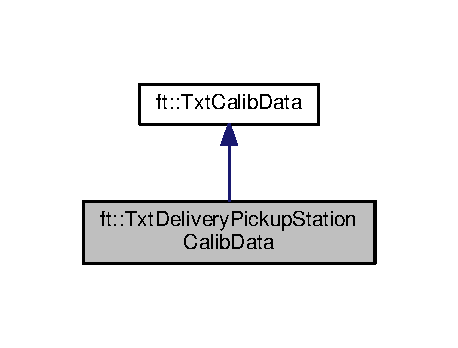
\includegraphics[width=220pt]{classft_1_1_txt_delivery_pickup_station_calib_data__inherit__graph}
\end{center}
\end{figure}


Collaboration diagram for ft\+:\+:Txt\+Delivery\+Pickup\+Station\+Calib\+Data\+:
\nopagebreak
\begin{figure}[H]
\begin{center}
\leavevmode
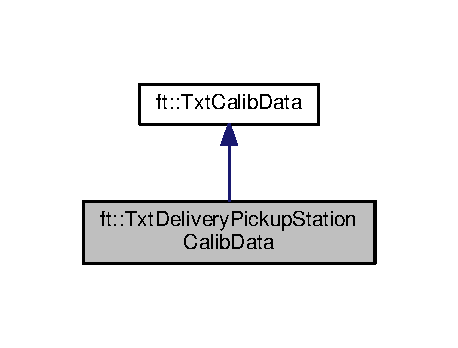
\includegraphics[width=220pt]{classft_1_1_txt_delivery_pickup_station_calib_data__coll__graph}
\end{center}
\end{figure}
\subsection*{Public Member Functions}
\begin{DoxyCompactItemize}
\item 
\hyperlink{classft_1_1_txt_delivery_pickup_station_calib_data_a7fe31c3fdbb44a72554a2fcdc9eec91e}{Txt\+Delivery\+Pickup\+Station\+Calib\+Data} ()
\item 
virtual \hyperlink{classft_1_1_txt_delivery_pickup_station_calib_data_a1411ad906d5fb22c0e025cdff543b594}{$\sim$\+Txt\+Delivery\+Pickup\+Station\+Calib\+Data} ()
\item 
bool \hyperlink{classft_1_1_txt_delivery_pickup_station_calib_data_a6bb1679754a7cb50ef455a0b1241c08a}{load} ()
\item 
bool \hyperlink{classft_1_1_txt_delivery_pickup_station_calib_data_a1cf9b3eb2a58d76ef84de23021c4e3bb}{save\+Default} ()
\item 
bool \hyperlink{classft_1_1_txt_delivery_pickup_station_calib_data_a0d4f07c8ccbb254d8bc1d2b431790717}{save} ()
\end{DoxyCompactItemize}
\subsection*{Public Attributes}
\begin{DoxyCompactItemize}
\item 
int \hyperlink{classft_1_1_txt_delivery_pickup_station_calib_data_a35809cf5b3c77bbcbf2c36c7905d286f}{color\+\_\+th} \mbox{[}2\mbox{]}
\item 
std\+::string \hyperlink{classft_1_1_txt_delivery_pickup_station_calib_data_a4cd1ea7a4ffc6e5a66d7cab90be86bb0}{uid\+\_\+actions} \mbox{[}5\mbox{]}
\end{DoxyCompactItemize}
\subsection*{Additional Inherited Members}


\subsection{Constructor \& Destructor Documentation}
\index{ft\+::\+Txt\+Delivery\+Pickup\+Station\+Calib\+Data@{ft\+::\+Txt\+Delivery\+Pickup\+Station\+Calib\+Data}!Txt\+Delivery\+Pickup\+Station\+Calib\+Data@{Txt\+Delivery\+Pickup\+Station\+Calib\+Data}}
\index{Txt\+Delivery\+Pickup\+Station\+Calib\+Data@{Txt\+Delivery\+Pickup\+Station\+Calib\+Data}!ft\+::\+Txt\+Delivery\+Pickup\+Station\+Calib\+Data@{ft\+::\+Txt\+Delivery\+Pickup\+Station\+Calib\+Data}}
\subsubsection[{\texorpdfstring{Txt\+Delivery\+Pickup\+Station\+Calib\+Data()}{TxtDeliveryPickupStationCalibData()}}]{\setlength{\rightskip}{0pt plus 5cm}ft\+::\+Txt\+Delivery\+Pickup\+Station\+Calib\+Data\+::\+Txt\+Delivery\+Pickup\+Station\+Calib\+Data (
\begin{DoxyParamCaption}
{}
\end{DoxyParamCaption}
)\hspace{0.3cm}{\ttfamily [inline]}}\hypertarget{classft_1_1_txt_delivery_pickup_station_calib_data_a7fe31c3fdbb44a72554a2fcdc9eec91e}{}\label{classft_1_1_txt_delivery_pickup_station_calib_data_a7fe31c3fdbb44a72554a2fcdc9eec91e}
\index{ft\+::\+Txt\+Delivery\+Pickup\+Station\+Calib\+Data@{ft\+::\+Txt\+Delivery\+Pickup\+Station\+Calib\+Data}!````~Txt\+Delivery\+Pickup\+Station\+Calib\+Data@{$\sim$\+Txt\+Delivery\+Pickup\+Station\+Calib\+Data}}
\index{````~Txt\+Delivery\+Pickup\+Station\+Calib\+Data@{$\sim$\+Txt\+Delivery\+Pickup\+Station\+Calib\+Data}!ft\+::\+Txt\+Delivery\+Pickup\+Station\+Calib\+Data@{ft\+::\+Txt\+Delivery\+Pickup\+Station\+Calib\+Data}}
\subsubsection[{\texorpdfstring{$\sim$\+Txt\+Delivery\+Pickup\+Station\+Calib\+Data()}{~TxtDeliveryPickupStationCalibData()}}]{\setlength{\rightskip}{0pt plus 5cm}virtual ft\+::\+Txt\+Delivery\+Pickup\+Station\+Calib\+Data\+::$\sim$\+Txt\+Delivery\+Pickup\+Station\+Calib\+Data (
\begin{DoxyParamCaption}
{}
\end{DoxyParamCaption}
)\hspace{0.3cm}{\ttfamily [inline]}, {\ttfamily [virtual]}}\hypertarget{classft_1_1_txt_delivery_pickup_station_calib_data_a1411ad906d5fb22c0e025cdff543b594}{}\label{classft_1_1_txt_delivery_pickup_station_calib_data_a1411ad906d5fb22c0e025cdff543b594}


\subsection{Member Function Documentation}
\index{ft\+::\+Txt\+Delivery\+Pickup\+Station\+Calib\+Data@{ft\+::\+Txt\+Delivery\+Pickup\+Station\+Calib\+Data}!load@{load}}
\index{load@{load}!ft\+::\+Txt\+Delivery\+Pickup\+Station\+Calib\+Data@{ft\+::\+Txt\+Delivery\+Pickup\+Station\+Calib\+Data}}
\subsubsection[{\texorpdfstring{load()}{load()}}]{\setlength{\rightskip}{0pt plus 5cm}bool ft\+::\+Txt\+Delivery\+Pickup\+Station\+Calib\+Data\+::load (
\begin{DoxyParamCaption}
{}
\end{DoxyParamCaption}
)\hspace{0.3cm}{\ttfamily [virtual]}}\hypertarget{classft_1_1_txt_delivery_pickup_station_calib_data_a6bb1679754a7cb50ef455a0b1241c08a}{}\label{classft_1_1_txt_delivery_pickup_station_calib_data_a6bb1679754a7cb50ef455a0b1241c08a}


Implements \hyperlink{classft_1_1_txt_calib_data_abe888396c95ead8fd554fc77ba486e7a}{ft\+::\+Txt\+Calib\+Data}.

\index{ft\+::\+Txt\+Delivery\+Pickup\+Station\+Calib\+Data@{ft\+::\+Txt\+Delivery\+Pickup\+Station\+Calib\+Data}!save@{save}}
\index{save@{save}!ft\+::\+Txt\+Delivery\+Pickup\+Station\+Calib\+Data@{ft\+::\+Txt\+Delivery\+Pickup\+Station\+Calib\+Data}}
\subsubsection[{\texorpdfstring{save()}{save()}}]{\setlength{\rightskip}{0pt plus 5cm}bool ft\+::\+Txt\+Delivery\+Pickup\+Station\+Calib\+Data\+::save (
\begin{DoxyParamCaption}
{}
\end{DoxyParamCaption}
)\hspace{0.3cm}{\ttfamily [virtual]}}\hypertarget{classft_1_1_txt_delivery_pickup_station_calib_data_a0d4f07c8ccbb254d8bc1d2b431790717}{}\label{classft_1_1_txt_delivery_pickup_station_calib_data_a0d4f07c8ccbb254d8bc1d2b431790717}


Implements \hyperlink{classft_1_1_txt_calib_data_a68a7bd5bfc32ebf82dd1a4fbe086a1b3}{ft\+::\+Txt\+Calib\+Data}.

\index{ft\+::\+Txt\+Delivery\+Pickup\+Station\+Calib\+Data@{ft\+::\+Txt\+Delivery\+Pickup\+Station\+Calib\+Data}!save\+Default@{save\+Default}}
\index{save\+Default@{save\+Default}!ft\+::\+Txt\+Delivery\+Pickup\+Station\+Calib\+Data@{ft\+::\+Txt\+Delivery\+Pickup\+Station\+Calib\+Data}}
\subsubsection[{\texorpdfstring{save\+Default()}{saveDefault()}}]{\setlength{\rightskip}{0pt plus 5cm}bool ft\+::\+Txt\+Delivery\+Pickup\+Station\+Calib\+Data\+::save\+Default (
\begin{DoxyParamCaption}
{}
\end{DoxyParamCaption}
)\hspace{0.3cm}{\ttfamily [virtual]}}\hypertarget{classft_1_1_txt_delivery_pickup_station_calib_data_a1cf9b3eb2a58d76ef84de23021c4e3bb}{}\label{classft_1_1_txt_delivery_pickup_station_calib_data_a1cf9b3eb2a58d76ef84de23021c4e3bb}


Implements \hyperlink{classft_1_1_txt_calib_data_aace95b90ba43836acbd8f0cf1dd323c7}{ft\+::\+Txt\+Calib\+Data}.



\subsection{Member Data Documentation}
\index{ft\+::\+Txt\+Delivery\+Pickup\+Station\+Calib\+Data@{ft\+::\+Txt\+Delivery\+Pickup\+Station\+Calib\+Data}!color\+\_\+th@{color\+\_\+th}}
\index{color\+\_\+th@{color\+\_\+th}!ft\+::\+Txt\+Delivery\+Pickup\+Station\+Calib\+Data@{ft\+::\+Txt\+Delivery\+Pickup\+Station\+Calib\+Data}}
\subsubsection[{\texorpdfstring{color\+\_\+th}{color_th}}]{\setlength{\rightskip}{0pt plus 5cm}int ft\+::\+Txt\+Delivery\+Pickup\+Station\+Calib\+Data\+::color\+\_\+th\mbox{[}2\mbox{]}}\hypertarget{classft_1_1_txt_delivery_pickup_station_calib_data_a35809cf5b3c77bbcbf2c36c7905d286f}{}\label{classft_1_1_txt_delivery_pickup_station_calib_data_a35809cf5b3c77bbcbf2c36c7905d286f}
\index{ft\+::\+Txt\+Delivery\+Pickup\+Station\+Calib\+Data@{ft\+::\+Txt\+Delivery\+Pickup\+Station\+Calib\+Data}!uid\+\_\+actions@{uid\+\_\+actions}}
\index{uid\+\_\+actions@{uid\+\_\+actions}!ft\+::\+Txt\+Delivery\+Pickup\+Station\+Calib\+Data@{ft\+::\+Txt\+Delivery\+Pickup\+Station\+Calib\+Data}}
\subsubsection[{\texorpdfstring{uid\+\_\+actions}{uid_actions}}]{\setlength{\rightskip}{0pt plus 5cm}std\+::string ft\+::\+Txt\+Delivery\+Pickup\+Station\+Calib\+Data\+::uid\+\_\+actions\mbox{[}5\mbox{]}}\hypertarget{classft_1_1_txt_delivery_pickup_station_calib_data_a4cd1ea7a4ffc6e5a66d7cab90be86bb0}{}\label{classft_1_1_txt_delivery_pickup_station_calib_data_a4cd1ea7a4ffc6e5a66d7cab90be86bb0}


The documentation for this class was generated from the following file\+:\begin{DoxyCompactItemize}
\item 
\hyperlink{_txt_delivery_pickup_station_8h}{Txt\+Delivery\+Pickup\+Station.\+h}\end{DoxyCompactItemize}

\hypertarget{classft_1_1_txt_delivery_pickup_station_observer}{}\section{ft\+:\+:Txt\+Delivery\+Pickup\+Station\+Observer Class Reference}
\label{classft_1_1_txt_delivery_pickup_station_observer}\index{ft\+::\+Txt\+Delivery\+Pickup\+Station\+Observer@{ft\+::\+Txt\+Delivery\+Pickup\+Station\+Observer}}


{\ttfamily \#include $<$Txt\+Delivery\+Pickup\+Station.\+h$>$}



Inheritance diagram for ft\+:\+:Txt\+Delivery\+Pickup\+Station\+Observer\+:
\nopagebreak
\begin{figure}[H]
\begin{center}
\leavevmode
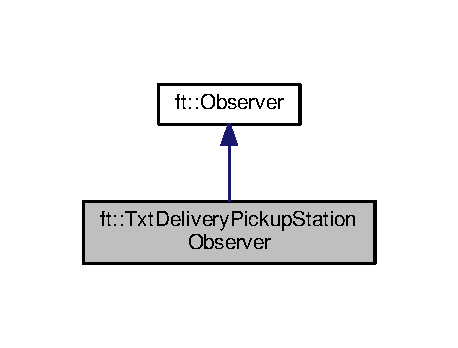
\includegraphics[width=220pt]{classft_1_1_txt_delivery_pickup_station_observer__inherit__graph}
\end{center}
\end{figure}


Collaboration diagram for ft\+:\+:Txt\+Delivery\+Pickup\+Station\+Observer\+:
\nopagebreak
\begin{figure}[H]
\begin{center}
\leavevmode
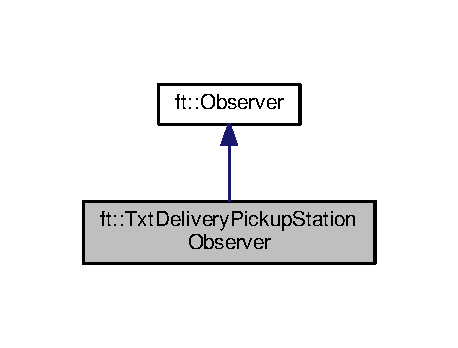
\includegraphics[width=220pt]{classft_1_1_txt_delivery_pickup_station_observer__coll__graph}
\end{center}
\end{figure}
\subsection*{Public Member Functions}
\begin{DoxyCompactItemize}
\item 
\hyperlink{classft_1_1_txt_delivery_pickup_station_observer_a1d5b30b54ab8f3368b97be5688daf03a}{Txt\+Delivery\+Pickup\+Station\+Observer} (\hyperlink{classft_1_1_txt_delivery_pickup_station}{ft\+::\+Txt\+Delivery\+Pickup\+Station} $\ast$s, \hyperlink{classft_1_1_txt_mqtt_factory_client}{ft\+::\+Txt\+Mqtt\+Factory\+Client} $\ast$mqttclient)
\item 
virtual \hyperlink{classft_1_1_txt_delivery_pickup_station_observer_a80913e3aef8fee4a1e8bcb9eeb46915d}{$\sim$\+Txt\+Delivery\+Pickup\+Station\+Observer} ()
\item 
void \hyperlink{classft_1_1_txt_delivery_pickup_station_observer_a2525d061949c0b3c282b485c7ee0592b}{Update} (\hyperlink{classft_1_1_subject_observer}{ft\+::\+Subject\+Observer} $\ast$the\+Changed\+Subject)
\end{DoxyCompactItemize}


\subsection{Constructor \& Destructor Documentation}
\index{ft\+::\+Txt\+Delivery\+Pickup\+Station\+Observer@{ft\+::\+Txt\+Delivery\+Pickup\+Station\+Observer}!Txt\+Delivery\+Pickup\+Station\+Observer@{Txt\+Delivery\+Pickup\+Station\+Observer}}
\index{Txt\+Delivery\+Pickup\+Station\+Observer@{Txt\+Delivery\+Pickup\+Station\+Observer}!ft\+::\+Txt\+Delivery\+Pickup\+Station\+Observer@{ft\+::\+Txt\+Delivery\+Pickup\+Station\+Observer}}
\subsubsection[{\texorpdfstring{Txt\+Delivery\+Pickup\+Station\+Observer(ft\+::\+Txt\+Delivery\+Pickup\+Station $\ast$s, ft\+::\+Txt\+Mqtt\+Factory\+Client $\ast$mqttclient)}{TxtDeliveryPickupStationObserver(ft::TxtDeliveryPickupStation *s, ft::TxtMqttFactoryClient *mqttclient)}}]{\setlength{\rightskip}{0pt plus 5cm}ft\+::\+Txt\+Delivery\+Pickup\+Station\+Observer\+::\+Txt\+Delivery\+Pickup\+Station\+Observer (
\begin{DoxyParamCaption}
\item[{{\bf ft\+::\+Txt\+Delivery\+Pickup\+Station} $\ast$}]{s, }
\item[{{\bf ft\+::\+Txt\+Mqtt\+Factory\+Client} $\ast$}]{mqttclient}
\end{DoxyParamCaption}
)\hspace{0.3cm}{\ttfamily [inline]}}\hypertarget{classft_1_1_txt_delivery_pickup_station_observer_a1d5b30b54ab8f3368b97be5688daf03a}{}\label{classft_1_1_txt_delivery_pickup_station_observer_a1d5b30b54ab8f3368b97be5688daf03a}
\index{ft\+::\+Txt\+Delivery\+Pickup\+Station\+Observer@{ft\+::\+Txt\+Delivery\+Pickup\+Station\+Observer}!````~Txt\+Delivery\+Pickup\+Station\+Observer@{$\sim$\+Txt\+Delivery\+Pickup\+Station\+Observer}}
\index{````~Txt\+Delivery\+Pickup\+Station\+Observer@{$\sim$\+Txt\+Delivery\+Pickup\+Station\+Observer}!ft\+::\+Txt\+Delivery\+Pickup\+Station\+Observer@{ft\+::\+Txt\+Delivery\+Pickup\+Station\+Observer}}
\subsubsection[{\texorpdfstring{$\sim$\+Txt\+Delivery\+Pickup\+Station\+Observer()}{~TxtDeliveryPickupStationObserver()}}]{\setlength{\rightskip}{0pt plus 5cm}virtual ft\+::\+Txt\+Delivery\+Pickup\+Station\+Observer\+::$\sim$\+Txt\+Delivery\+Pickup\+Station\+Observer (
\begin{DoxyParamCaption}
{}
\end{DoxyParamCaption}
)\hspace{0.3cm}{\ttfamily [inline]}, {\ttfamily [virtual]}}\hypertarget{classft_1_1_txt_delivery_pickup_station_observer_a80913e3aef8fee4a1e8bcb9eeb46915d}{}\label{classft_1_1_txt_delivery_pickup_station_observer_a80913e3aef8fee4a1e8bcb9eeb46915d}


\subsection{Member Function Documentation}
\index{ft\+::\+Txt\+Delivery\+Pickup\+Station\+Observer@{ft\+::\+Txt\+Delivery\+Pickup\+Station\+Observer}!Update@{Update}}
\index{Update@{Update}!ft\+::\+Txt\+Delivery\+Pickup\+Station\+Observer@{ft\+::\+Txt\+Delivery\+Pickup\+Station\+Observer}}
\subsubsection[{\texorpdfstring{Update(ft\+::\+Subject\+Observer $\ast$the\+Changed\+Subject)}{Update(ft::SubjectObserver *theChangedSubject)}}]{\setlength{\rightskip}{0pt plus 5cm}void ft\+::\+Txt\+Delivery\+Pickup\+Station\+Observer\+::\+Update (
\begin{DoxyParamCaption}
\item[{{\bf ft\+::\+Subject\+Observer} $\ast$}]{the\+Changed\+Subject}
\end{DoxyParamCaption}
)\hspace{0.3cm}{\ttfamily [inline]}, {\ttfamily [virtual]}}\hypertarget{classft_1_1_txt_delivery_pickup_station_observer_a2525d061949c0b3c282b485c7ee0592b}{}\label{classft_1_1_txt_delivery_pickup_station_observer_a2525d061949c0b3c282b485c7ee0592b}


Implements \hyperlink{classft_1_1_observer_aeea41c77afbd09f595a4290954a5aa66}{ft\+::\+Observer}.



The documentation for this class was generated from the following file\+:\begin{DoxyCompactItemize}
\item 
\hyperlink{_txt_delivery_pickup_station_8h}{Txt\+Delivery\+Pickup\+Station.\+h}\end{DoxyCompactItemize}

\hypertarget{classft_1_1_txt_factory_process_storage}{}\section{ft\+:\+:Txt\+Factory\+Process\+Storage Class Reference}
\label{classft_1_1_txt_factory_process_storage}\index{ft\+::\+Txt\+Factory\+Process\+Storage@{ft\+::\+Txt\+Factory\+Process\+Storage}}


{\ttfamily \#include $<$Txt\+Factory\+Process\+Storage.\+h$>$}

\subsection*{Public Member Functions}
\begin{DoxyCompactItemize}
\item 
\hyperlink{classft_1_1_txt_factory_process_storage_a0e88aec0c0f9dc6e00de46ecdb833adc}{Txt\+Factory\+Process\+Storage} ()
\item 
virtual \hyperlink{classft_1_1_txt_factory_process_storage_a52e8ba413486356acd2d218204ea5f10}{$\sim$\+Txt\+Factory\+Process\+Storage} ()
\item 
void \hyperlink{classft_1_1_txt_factory_process_storage_a460fae87650acf9a261efbb04907d90a}{set\+Timestamp\+Now} (const std\+::string tag\+\_\+uid, \hyperlink{namespaceft_a87eb4112317a6f3c7ade8f26b6f8c1c8}{Txt\+History\+Index\+\_\+t} i)
\item 
std\+::vector$<$ int64\+\_\+t $>$ \hyperlink{classft_1_1_txt_factory_process_storage_a9884d553f0f777b7c1e808ae544ec55a}{get\+Tag\+Uid\+Vts} (const std\+::string tag\+\_\+uid)
\item 
uint8\+\_\+t \hyperlink{classft_1_1_txt_factory_process_storage_a5a1c6bd13e95364f47ffc75b1854a455}{get\+Tag\+Uid\+Mask\+Ts} (const std\+::string tag\+\_\+uid)
\item 
void \hyperlink{classft_1_1_txt_factory_process_storage_a98be66a6ae2ab4ab312adae2b0203545}{reset\+Tag\+Uid\+Mask\+Ts} (const std\+::string tag\+\_\+uid)
\end{DoxyCompactItemize}
\subsection*{Protected Member Functions}
\begin{DoxyCompactItemize}
\item 
void \hyperlink{classft_1_1_txt_factory_process_storage_a5150437507748d2c569becdd0359fc31}{print\+Map} ()
\end{DoxyCompactItemize}
\subsection*{Protected Attributes}
\begin{DoxyCompactItemize}
\item 
std\+::map$<$ std\+::string, std\+::vector$<$ int64\+\_\+t $>$ $>$ \hyperlink{classft_1_1_txt_factory_process_storage_a161c958fb54ded7f486fd20bd5348c42}{map\+\_\+vts}
\item 
std\+::map$<$ std\+::string, uint8\+\_\+t $>$ \hyperlink{classft_1_1_txt_factory_process_storage_a343110030a220d5ab36663cbe5ed38f5}{map\+\_\+mask\+\_\+ts}
\end{DoxyCompactItemize}


\subsection{Constructor \& Destructor Documentation}
\index{ft\+::\+Txt\+Factory\+Process\+Storage@{ft\+::\+Txt\+Factory\+Process\+Storage}!Txt\+Factory\+Process\+Storage@{Txt\+Factory\+Process\+Storage}}
\index{Txt\+Factory\+Process\+Storage@{Txt\+Factory\+Process\+Storage}!ft\+::\+Txt\+Factory\+Process\+Storage@{ft\+::\+Txt\+Factory\+Process\+Storage}}
\subsubsection[{\texorpdfstring{Txt\+Factory\+Process\+Storage()}{TxtFactoryProcessStorage()}}]{\setlength{\rightskip}{0pt plus 5cm}ft\+::\+Txt\+Factory\+Process\+Storage\+::\+Txt\+Factory\+Process\+Storage (
\begin{DoxyParamCaption}
{}
\end{DoxyParamCaption}
)}\hypertarget{classft_1_1_txt_factory_process_storage_a0e88aec0c0f9dc6e00de46ecdb833adc}{}\label{classft_1_1_txt_factory_process_storage_a0e88aec0c0f9dc6e00de46ecdb833adc}
\index{ft\+::\+Txt\+Factory\+Process\+Storage@{ft\+::\+Txt\+Factory\+Process\+Storage}!````~Txt\+Factory\+Process\+Storage@{$\sim$\+Txt\+Factory\+Process\+Storage}}
\index{````~Txt\+Factory\+Process\+Storage@{$\sim$\+Txt\+Factory\+Process\+Storage}!ft\+::\+Txt\+Factory\+Process\+Storage@{ft\+::\+Txt\+Factory\+Process\+Storage}}
\subsubsection[{\texorpdfstring{$\sim$\+Txt\+Factory\+Process\+Storage()}{~TxtFactoryProcessStorage()}}]{\setlength{\rightskip}{0pt plus 5cm}virtual ft\+::\+Txt\+Factory\+Process\+Storage\+::$\sim$\+Txt\+Factory\+Process\+Storage (
\begin{DoxyParamCaption}
{}
\end{DoxyParamCaption}
)\hspace{0.3cm}{\ttfamily [virtual]}}\hypertarget{classft_1_1_txt_factory_process_storage_a52e8ba413486356acd2d218204ea5f10}{}\label{classft_1_1_txt_factory_process_storage_a52e8ba413486356acd2d218204ea5f10}


\subsection{Member Function Documentation}
\index{ft\+::\+Txt\+Factory\+Process\+Storage@{ft\+::\+Txt\+Factory\+Process\+Storage}!get\+Tag\+Uid\+Mask\+Ts@{get\+Tag\+Uid\+Mask\+Ts}}
\index{get\+Tag\+Uid\+Mask\+Ts@{get\+Tag\+Uid\+Mask\+Ts}!ft\+::\+Txt\+Factory\+Process\+Storage@{ft\+::\+Txt\+Factory\+Process\+Storage}}
\subsubsection[{\texorpdfstring{get\+Tag\+Uid\+Mask\+Ts(const std\+::string tag\+\_\+uid)}{getTagUidMaskTs(const std::string tag_uid)}}]{\setlength{\rightskip}{0pt plus 5cm}uint8\+\_\+t ft\+::\+Txt\+Factory\+Process\+Storage\+::get\+Tag\+Uid\+Mask\+Ts (
\begin{DoxyParamCaption}
\item[{const std\+::string}]{tag\+\_\+uid}
\end{DoxyParamCaption}
)}\hypertarget{classft_1_1_txt_factory_process_storage_a5a1c6bd13e95364f47ffc75b1854a455}{}\label{classft_1_1_txt_factory_process_storage_a5a1c6bd13e95364f47ffc75b1854a455}
\index{ft\+::\+Txt\+Factory\+Process\+Storage@{ft\+::\+Txt\+Factory\+Process\+Storage}!get\+Tag\+Uid\+Vts@{get\+Tag\+Uid\+Vts}}
\index{get\+Tag\+Uid\+Vts@{get\+Tag\+Uid\+Vts}!ft\+::\+Txt\+Factory\+Process\+Storage@{ft\+::\+Txt\+Factory\+Process\+Storage}}
\subsubsection[{\texorpdfstring{get\+Tag\+Uid\+Vts(const std\+::string tag\+\_\+uid)}{getTagUidVts(const std::string tag_uid)}}]{\setlength{\rightskip}{0pt plus 5cm}std\+::vector$<$int64\+\_\+t$>$ ft\+::\+Txt\+Factory\+Process\+Storage\+::get\+Tag\+Uid\+Vts (
\begin{DoxyParamCaption}
\item[{const std\+::string}]{tag\+\_\+uid}
\end{DoxyParamCaption}
)}\hypertarget{classft_1_1_txt_factory_process_storage_a9884d553f0f777b7c1e808ae544ec55a}{}\label{classft_1_1_txt_factory_process_storage_a9884d553f0f777b7c1e808ae544ec55a}
\index{ft\+::\+Txt\+Factory\+Process\+Storage@{ft\+::\+Txt\+Factory\+Process\+Storage}!print\+Map@{print\+Map}}
\index{print\+Map@{print\+Map}!ft\+::\+Txt\+Factory\+Process\+Storage@{ft\+::\+Txt\+Factory\+Process\+Storage}}
\subsubsection[{\texorpdfstring{print\+Map()}{printMap()}}]{\setlength{\rightskip}{0pt plus 5cm}void ft\+::\+Txt\+Factory\+Process\+Storage\+::print\+Map (
\begin{DoxyParamCaption}
{}
\end{DoxyParamCaption}
)\hspace{0.3cm}{\ttfamily [protected]}}\hypertarget{classft_1_1_txt_factory_process_storage_a5150437507748d2c569becdd0359fc31}{}\label{classft_1_1_txt_factory_process_storage_a5150437507748d2c569becdd0359fc31}
\index{ft\+::\+Txt\+Factory\+Process\+Storage@{ft\+::\+Txt\+Factory\+Process\+Storage}!reset\+Tag\+Uid\+Mask\+Ts@{reset\+Tag\+Uid\+Mask\+Ts}}
\index{reset\+Tag\+Uid\+Mask\+Ts@{reset\+Tag\+Uid\+Mask\+Ts}!ft\+::\+Txt\+Factory\+Process\+Storage@{ft\+::\+Txt\+Factory\+Process\+Storage}}
\subsubsection[{\texorpdfstring{reset\+Tag\+Uid\+Mask\+Ts(const std\+::string tag\+\_\+uid)}{resetTagUidMaskTs(const std::string tag_uid)}}]{\setlength{\rightskip}{0pt plus 5cm}void ft\+::\+Txt\+Factory\+Process\+Storage\+::reset\+Tag\+Uid\+Mask\+Ts (
\begin{DoxyParamCaption}
\item[{const std\+::string}]{tag\+\_\+uid}
\end{DoxyParamCaption}
)}\hypertarget{classft_1_1_txt_factory_process_storage_a98be66a6ae2ab4ab312adae2b0203545}{}\label{classft_1_1_txt_factory_process_storage_a98be66a6ae2ab4ab312adae2b0203545}
\index{ft\+::\+Txt\+Factory\+Process\+Storage@{ft\+::\+Txt\+Factory\+Process\+Storage}!set\+Timestamp\+Now@{set\+Timestamp\+Now}}
\index{set\+Timestamp\+Now@{set\+Timestamp\+Now}!ft\+::\+Txt\+Factory\+Process\+Storage@{ft\+::\+Txt\+Factory\+Process\+Storage}}
\subsubsection[{\texorpdfstring{set\+Timestamp\+Now(const std\+::string tag\+\_\+uid, Txt\+History\+Index\+\_\+t i)}{setTimestampNow(const std::string tag_uid, TxtHistoryIndex_t i)}}]{\setlength{\rightskip}{0pt plus 5cm}void ft\+::\+Txt\+Factory\+Process\+Storage\+::set\+Timestamp\+Now (
\begin{DoxyParamCaption}
\item[{const std\+::string}]{tag\+\_\+uid, }
\item[{{\bf Txt\+History\+Index\+\_\+t}}]{i}
\end{DoxyParamCaption}
)}\hypertarget{classft_1_1_txt_factory_process_storage_a460fae87650acf9a261efbb04907d90a}{}\label{classft_1_1_txt_factory_process_storage_a460fae87650acf9a261efbb04907d90a}


\subsection{Member Data Documentation}
\index{ft\+::\+Txt\+Factory\+Process\+Storage@{ft\+::\+Txt\+Factory\+Process\+Storage}!map\+\_\+mask\+\_\+ts@{map\+\_\+mask\+\_\+ts}}
\index{map\+\_\+mask\+\_\+ts@{map\+\_\+mask\+\_\+ts}!ft\+::\+Txt\+Factory\+Process\+Storage@{ft\+::\+Txt\+Factory\+Process\+Storage}}
\subsubsection[{\texorpdfstring{map\+\_\+mask\+\_\+ts}{map_mask_ts}}]{\setlength{\rightskip}{0pt plus 5cm}std\+::map$<$std\+::string, uint8\+\_\+t$>$ ft\+::\+Txt\+Factory\+Process\+Storage\+::map\+\_\+mask\+\_\+ts\hspace{0.3cm}{\ttfamily [protected]}}\hypertarget{classft_1_1_txt_factory_process_storage_a343110030a220d5ab36663cbe5ed38f5}{}\label{classft_1_1_txt_factory_process_storage_a343110030a220d5ab36663cbe5ed38f5}
\index{ft\+::\+Txt\+Factory\+Process\+Storage@{ft\+::\+Txt\+Factory\+Process\+Storage}!map\+\_\+vts@{map\+\_\+vts}}
\index{map\+\_\+vts@{map\+\_\+vts}!ft\+::\+Txt\+Factory\+Process\+Storage@{ft\+::\+Txt\+Factory\+Process\+Storage}}
\subsubsection[{\texorpdfstring{map\+\_\+vts}{map_vts}}]{\setlength{\rightskip}{0pt plus 5cm}std\+::map$<$std\+::string, std\+::vector$<$int64\+\_\+t$>$ $>$ ft\+::\+Txt\+Factory\+Process\+Storage\+::map\+\_\+vts\hspace{0.3cm}{\ttfamily [protected]}}\hypertarget{classft_1_1_txt_factory_process_storage_a161c958fb54ded7f486fd20bd5348c42}{}\label{classft_1_1_txt_factory_process_storage_a161c958fb54ded7f486fd20bd5348c42}


The documentation for this class was generated from the following file\+:\begin{DoxyCompactItemize}
\item 
\hyperlink{_txt_factory_process_storage_8h}{Txt\+Factory\+Process\+Storage.\+h}\end{DoxyCompactItemize}

\hypertarget{classft_1_1_txt_flapping}{}\section{ft\+:\+:Txt\+Flapping Class Reference}
\label{classft_1_1_txt_flapping}\index{ft\+::\+Txt\+Flapping@{ft\+::\+Txt\+Flapping}}


{\ttfamily \#include $<$Txt\+Alert.\+h$>$}

\subsection*{Public Member Functions}
\begin{DoxyCompactItemize}
\item 
\hyperlink{classft_1_1_txt_flapping_a67f2ea24c51dc22e4bfc16a34ac4f870}{Txt\+Flapping} ()
\item 
virtual \hyperlink{classft_1_1_txt_flapping_a77517485bbb60f3cc1ca0012f34c9eac}{$\sim$\+Txt\+Flapping} ()
\item 
void \hyperlink{classft_1_1_txt_flapping_ab65f5517cf7ed8b5f634758d47f65e67}{Update\+Flapping\+Status} (bool state\+Change)
\item 
bool \hyperlink{classft_1_1_txt_flapping_aa58fe28a9a01bfaffb54f19776b9889d}{Is\+Flapping} () const 
\end{DoxyCompactItemize}


\subsection{Constructor \& Destructor Documentation}
\index{ft\+::\+Txt\+Flapping@{ft\+::\+Txt\+Flapping}!Txt\+Flapping@{Txt\+Flapping}}
\index{Txt\+Flapping@{Txt\+Flapping}!ft\+::\+Txt\+Flapping@{ft\+::\+Txt\+Flapping}}
\subsubsection[{\texorpdfstring{Txt\+Flapping()}{TxtFlapping()}}]{\setlength{\rightskip}{0pt plus 5cm}ft\+::\+Txt\+Flapping\+::\+Txt\+Flapping (
\begin{DoxyParamCaption}
{}
\end{DoxyParamCaption}
)}\hypertarget{classft_1_1_txt_flapping_a67f2ea24c51dc22e4bfc16a34ac4f870}{}\label{classft_1_1_txt_flapping_a67f2ea24c51dc22e4bfc16a34ac4f870}
\index{ft\+::\+Txt\+Flapping@{ft\+::\+Txt\+Flapping}!````~Txt\+Flapping@{$\sim$\+Txt\+Flapping}}
\index{````~Txt\+Flapping@{$\sim$\+Txt\+Flapping}!ft\+::\+Txt\+Flapping@{ft\+::\+Txt\+Flapping}}
\subsubsection[{\texorpdfstring{$\sim$\+Txt\+Flapping()}{~TxtFlapping()}}]{\setlength{\rightskip}{0pt plus 5cm}virtual ft\+::\+Txt\+Flapping\+::$\sim$\+Txt\+Flapping (
\begin{DoxyParamCaption}
{}
\end{DoxyParamCaption}
)\hspace{0.3cm}{\ttfamily [virtual]}}\hypertarget{classft_1_1_txt_flapping_a77517485bbb60f3cc1ca0012f34c9eac}{}\label{classft_1_1_txt_flapping_a77517485bbb60f3cc1ca0012f34c9eac}


\subsection{Member Function Documentation}
\index{ft\+::\+Txt\+Flapping@{ft\+::\+Txt\+Flapping}!Is\+Flapping@{Is\+Flapping}}
\index{Is\+Flapping@{Is\+Flapping}!ft\+::\+Txt\+Flapping@{ft\+::\+Txt\+Flapping}}
\subsubsection[{\texorpdfstring{Is\+Flapping() const }{IsFlapping() const }}]{\setlength{\rightskip}{0pt plus 5cm}bool ft\+::\+Txt\+Flapping\+::\+Is\+Flapping (
\begin{DoxyParamCaption}
{}
\end{DoxyParamCaption}
) const\hspace{0.3cm}{\ttfamily [inline]}}\hypertarget{classft_1_1_txt_flapping_aa58fe28a9a01bfaffb54f19776b9889d}{}\label{classft_1_1_txt_flapping_aa58fe28a9a01bfaffb54f19776b9889d}
\index{ft\+::\+Txt\+Flapping@{ft\+::\+Txt\+Flapping}!Update\+Flapping\+Status@{Update\+Flapping\+Status}}
\index{Update\+Flapping\+Status@{Update\+Flapping\+Status}!ft\+::\+Txt\+Flapping@{ft\+::\+Txt\+Flapping}}
\subsubsection[{\texorpdfstring{Update\+Flapping\+Status(bool state\+Change)}{UpdateFlappingStatus(bool stateChange)}}]{\setlength{\rightskip}{0pt plus 5cm}void ft\+::\+Txt\+Flapping\+::\+Update\+Flapping\+Status (
\begin{DoxyParamCaption}
\item[{bool}]{state\+Change}
\end{DoxyParamCaption}
)}\hypertarget{classft_1_1_txt_flapping_ab65f5517cf7ed8b5f634758d47f65e67}{}\label{classft_1_1_txt_flapping_ab65f5517cf7ed8b5f634758d47f65e67}


The documentation for this class was generated from the following file\+:\begin{DoxyCompactItemize}
\item 
\hyperlink{_txt_alert_8h}{Txt\+Alert.\+h}\end{DoxyCompactItemize}

\hypertarget{classft_1_1_txt_high_bay_warehouse}{}\section{ft\+:\+:Txt\+High\+Bay\+Warehouse Class Reference}
\label{classft_1_1_txt_high_bay_warehouse}\index{ft\+::\+Txt\+High\+Bay\+Warehouse@{ft\+::\+Txt\+High\+Bay\+Warehouse}}


{\ttfamily \#include $<$Txt\+High\+Bay\+Warehouse.\+h$>$}



Inheritance diagram for ft\+:\+:Txt\+High\+Bay\+Warehouse\+:
\nopagebreak
\begin{figure}[H]
\begin{center}
\leavevmode
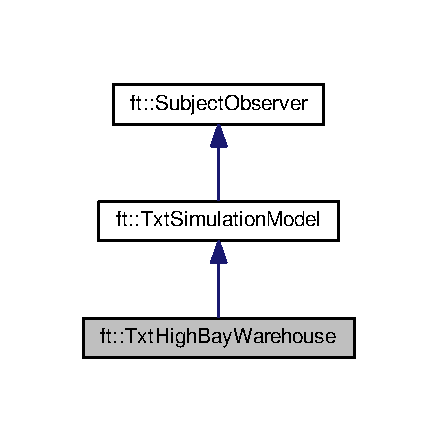
\includegraphics[width=210pt]{classft_1_1_txt_high_bay_warehouse__inherit__graph}
\end{center}
\end{figure}


Collaboration diagram for ft\+:\+:Txt\+High\+Bay\+Warehouse\+:
\nopagebreak
\begin{figure}[H]
\begin{center}
\leavevmode
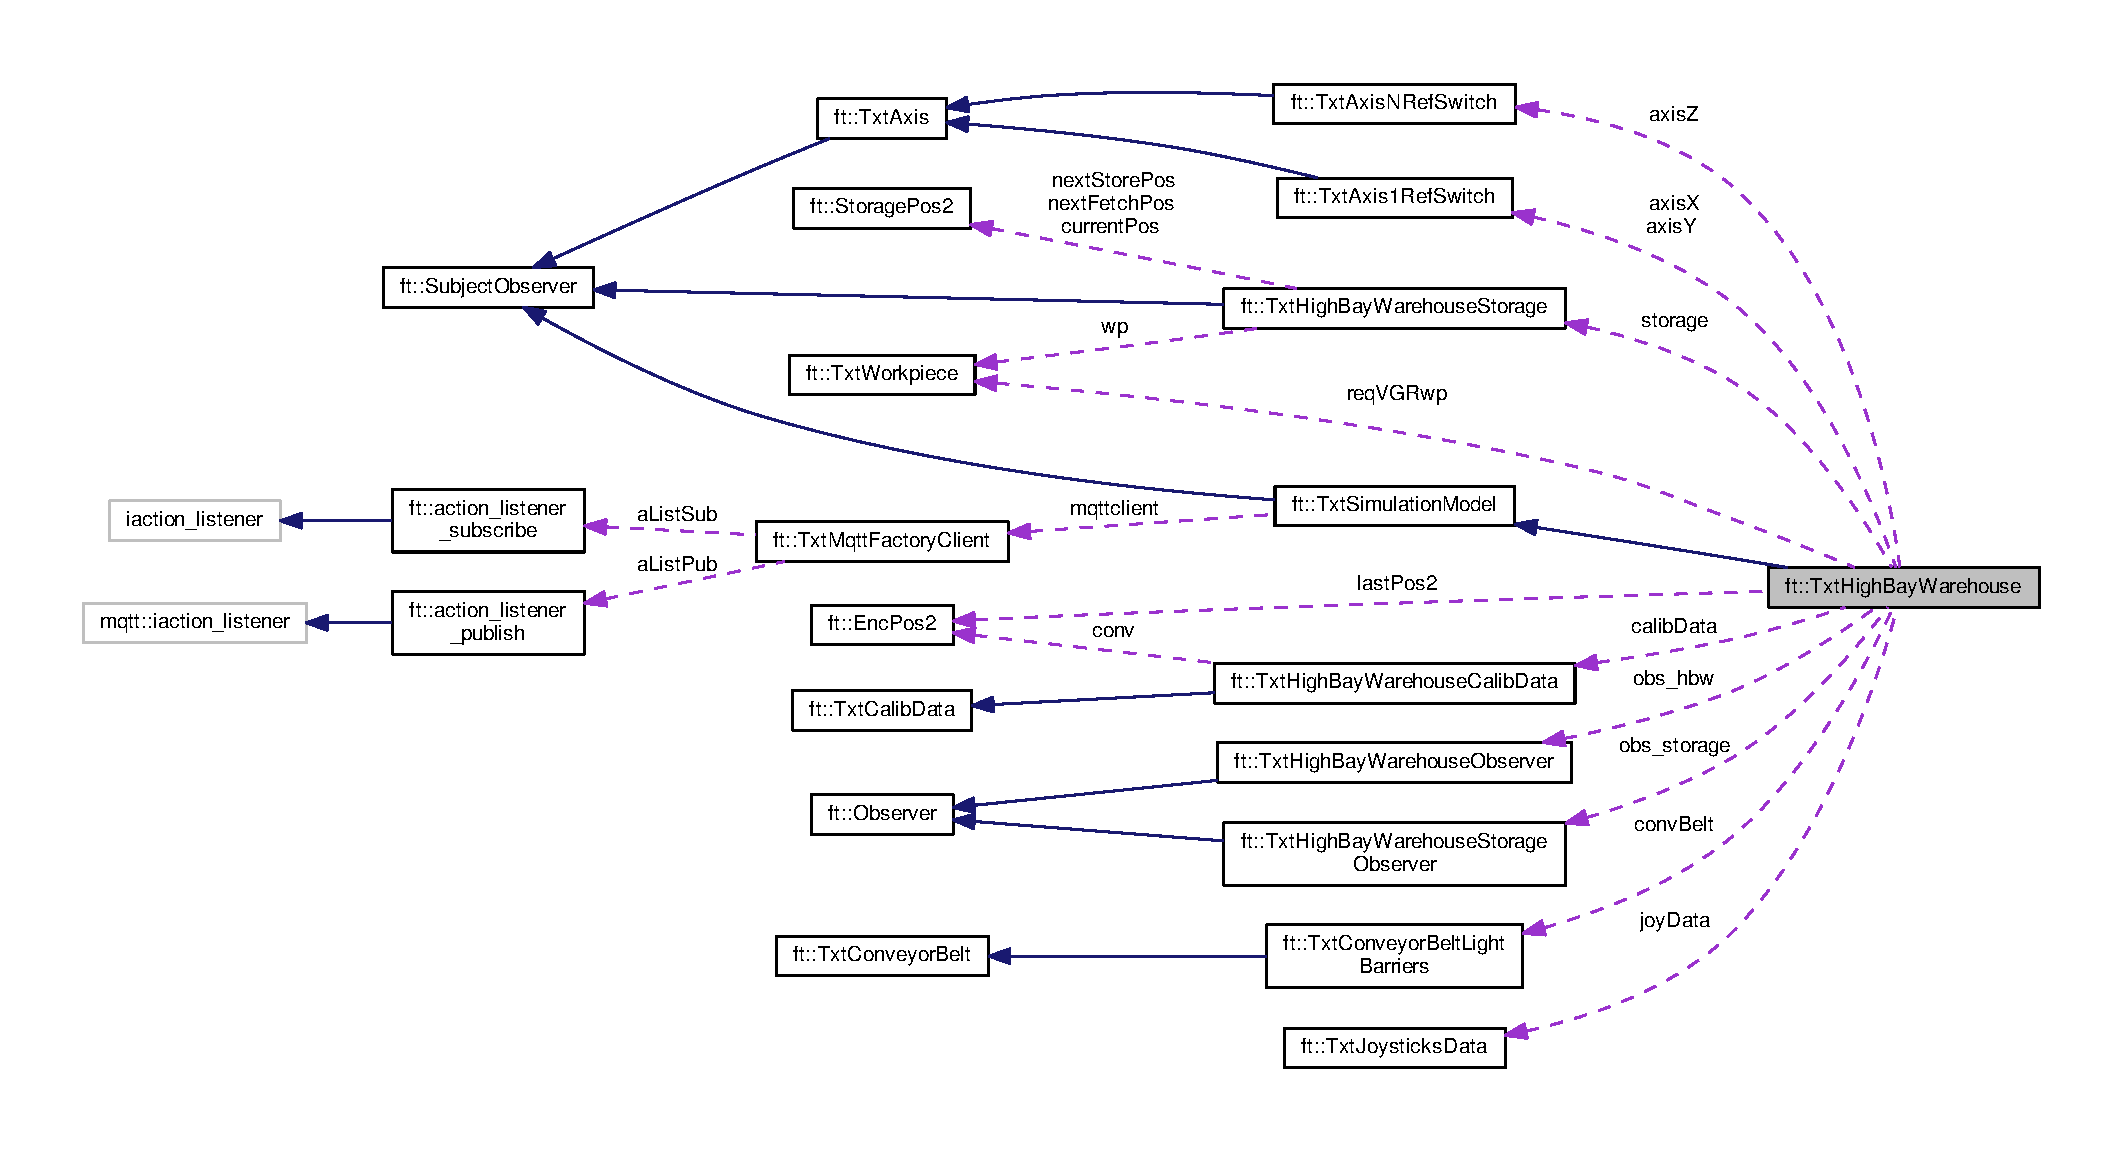
\includegraphics[width=350pt]{classft_1_1_txt_high_bay_warehouse__coll__graph}
\end{center}
\end{figure}
\subsection*{Public Types}
\begin{DoxyCompactItemize}
\item 
enum \hyperlink{classft_1_1_txt_high_bay_warehouse_aa35f35b5549913d838cb6070bb28da30}{State\+\_\+t} \{ \\*
\hyperlink{classft_1_1_txt_high_bay_warehouse_aa35f35b5549913d838cb6070bb28da30aff317df37e7b7e302038bf2ed5bb3d5b}{\+\_\+\+\_\+\+N\+O\+\_\+\+S\+T\+A\+TE}, 
\hyperlink{classft_1_1_txt_high_bay_warehouse_aa35f35b5549913d838cb6070bb28da30a5847b141b1088cf955c343c02bbfce10}{I\+D\+LE}, 
\hyperlink{classft_1_1_txt_high_bay_warehouse_aa35f35b5549913d838cb6070bb28da30a6283f682cffd01ff4225bdaaf6c1716e}{I\+N\+IT}, 
\hyperlink{classft_1_1_txt_high_bay_warehouse_aa35f35b5549913d838cb6070bb28da30a36a778abf469c5dc849a79a1f80e19a2}{F\+A\+U\+LT}, 
\\*
\hyperlink{classft_1_1_txt_high_bay_warehouse_aa35f35b5549913d838cb6070bb28da30a043ea37089e2b7f526c93834f59d3f84}{F\+E\+T\+C\+H\+\_\+\+C\+O\+N\+T\+A\+I\+N\+ER}, 
\hyperlink{classft_1_1_txt_high_bay_warehouse_aa35f35b5549913d838cb6070bb28da30a8a2cacacb28133e3c43c0d1a09a4c3bc}{S\+T\+O\+R\+E\+\_\+\+WP}, 
\hyperlink{classft_1_1_txt_high_bay_warehouse_aa35f35b5549913d838cb6070bb28da30a4a6f156de32d8c10cfc3ee78433f0f0c}{F\+E\+T\+C\+H\+\_\+\+WP}, 
\hyperlink{classft_1_1_txt_high_bay_warehouse_aa35f35b5549913d838cb6070bb28da30a5caa2fd64471651c7b8a018ddf3ef10c}{F\+E\+T\+C\+H\+\_\+\+W\+P\+\_\+\+W\+A\+IT}, 
\\*
\hyperlink{classft_1_1_txt_high_bay_warehouse_aa35f35b5549913d838cb6070bb28da30afc77ffa8e83b3e9940698351bcf73d3d}{S\+T\+O\+R\+E\+\_\+\+C\+O\+N\+T\+A\+I\+N\+ER}, 
\hyperlink{classft_1_1_txt_high_bay_warehouse_aa35f35b5549913d838cb6070bb28da30aae851127a9375cbbc073376e50a38d5a}{C\+A\+L\+I\+B\+\_\+\+H\+BW}, 
\hyperlink{classft_1_1_txt_high_bay_warehouse_aa35f35b5549913d838cb6070bb28da30a897ff36a4bf1229592cd94de50be2aed}{C\+A\+L\+I\+B\+\_\+\+N\+AV}, 
\hyperlink{classft_1_1_txt_high_bay_warehouse_aa35f35b5549913d838cb6070bb28da30ab3a82d97b39900e4b6f88ba98d84bd84}{C\+A\+L\+I\+B\+\_\+\+M\+O\+VE}
 \}
\end{DoxyCompactItemize}
\subsection*{Public Member Functions}
\begin{DoxyCompactItemize}
\item 
const char $\ast$ \hyperlink{classft_1_1_txt_high_bay_warehouse_abeb6f6eb81f6f14ebb9040c160acc625}{to\+String} (\hyperlink{classft_1_1_txt_high_bay_warehouse_aa35f35b5549913d838cb6070bb28da30}{State\+\_\+t} state)
\item 
void \hyperlink{classft_1_1_txt_high_bay_warehouse_a82187c81e5183dae8bf563556c5e6b37}{print\+State} (\hyperlink{classft_1_1_txt_high_bay_warehouse_aa35f35b5549913d838cb6070bb28da30}{State\+\_\+t} state)
\item 
void \hyperlink{classft_1_1_txt_high_bay_warehouse_a894191eac9f7824d017008eab5e95251}{print\+Entry\+State} (\hyperlink{classft_1_1_txt_high_bay_warehouse_aa35f35b5549913d838cb6070bb28da30}{State\+\_\+t} state)
\item 
void \hyperlink{classft_1_1_txt_high_bay_warehouse_aed345d897ebc62ba2cc86d8ecc3b43e9}{print\+Exit\+State} (\hyperlink{classft_1_1_txt_high_bay_warehouse_aa35f35b5549913d838cb6070bb28da30}{State\+\_\+t} state)
\item 
\hyperlink{classft_1_1_txt_high_bay_warehouse_a126ecc2341746fce3a9a2ae75fc1a72b}{Txt\+High\+Bay\+Warehouse} (F\+I\+S\+H\+\_\+\+X1\+\_\+\+T\+R\+A\+N\+S\+F\+ER $\ast$\hyperlink{classft_1_1_txt_simulation_model_a9facd66a0dbecd676ae7b72c37a0b300}{p\+T\+Area}, \hyperlink{classft_1_1_txt_mqtt_factory_client}{ft\+::\+Txt\+Mqtt\+Factory\+Client} $\ast$\hyperlink{classft_1_1_txt_simulation_model_a6a92fdef8619b9b1636c7c464091ea3a}{mqttclient})
\item 
virtual \hyperlink{classft_1_1_txt_high_bay_warehouse_a6a91915425a003402ad626d45b84a6e8}{$\sim$\+Txt\+High\+Bay\+Warehouse} ()
\item 
void \hyperlink{classft_1_1_txt_high_bay_warehouse_a8e8deaf93270532a80c6bc40390d2275}{request\+Quit} ()
\item 
void \hyperlink{classft_1_1_txt_high_bay_warehouse_a8c85ddf8678b0589ebbd1efd5c0a6833}{request\+V\+G\+Rfetch\+Container} (\hyperlink{classft_1_1_txt_workpiece}{Txt\+Workpiece} $\ast$wp)
\item 
void \hyperlink{classft_1_1_txt_high_bay_warehouse_a1da138b9b408d9ebfa8dca1c14558f8c}{request\+V\+G\+Rstore} (\hyperlink{classft_1_1_txt_workpiece}{Txt\+Workpiece} $\ast$wp)
\item 
void \hyperlink{classft_1_1_txt_high_bay_warehouse_a986d4c61e1666039dcedee24868578d7}{request\+V\+G\+Rfetch} (\hyperlink{classft_1_1_txt_workpiece}{Txt\+Workpiece} $\ast$wp)
\item 
void \hyperlink{classft_1_1_txt_high_bay_warehouse_a4321b39920184a1147017651286735dc}{request\+V\+G\+Rstore\+Container} (\hyperlink{classft_1_1_txt_workpiece}{Txt\+Workpiece} $\ast$wp)
\item 
void \hyperlink{classft_1_1_txt_high_bay_warehouse_a6556c4e1b0c1694a4e791f8bd66a6a11}{request\+V\+G\+Rcalib} ()
\item 
void \hyperlink{classft_1_1_txt_high_bay_warehouse_a1d0b36be0177afb2675db7354240d27a}{request\+V\+G\+Rreset\+Storage} ()
\item 
void \hyperlink{classft_1_1_txt_high_bay_warehouse_a54653fd5c84c7cbd7fd684511f4ca800}{request\+Joy\+But} (\hyperlink{classft_1_1_txt_joysticks_data}{Txt\+Joysticks\+Data} jd)
\item 
bool \hyperlink{classft_1_1_txt_high_bay_warehouse_a2a08665e626da0c946461e5df89937c2}{load\+Calib} ()
\item 
bool \hyperlink{classft_1_1_txt_high_bay_warehouse_ae6deca6a80680d0d563fde5296b618cb}{save\+Calib\+Default} ()
\item 
void \hyperlink{classft_1_1_txt_high_bay_warehouse_a486b766d3f8f11a023daee496429faf0}{stop} ()
\item 
void \hyperlink{classft_1_1_txt_high_bay_warehouse_ae18724814f18d63433a00058622c29bd}{move\+Ref} ()
\item 
\hyperlink{classft_1_1_enc_pos2}{Enc\+Pos2} \hyperlink{classft_1_1_txt_high_bay_warehouse_a1fcf0e88756f2665516b7e15cf4176a4}{get\+Pos2} ()
\item 
void \hyperlink{classft_1_1_txt_high_bay_warehouse_aa73dd2693ee1c2487509b7c82d9a1009}{move\+Joystick} ()
\item 
bool \hyperlink{classft_1_1_txt_high_bay_warehouse_afed1cdc629d97c3776acd48fbc737780}{store} (\hyperlink{classft_1_1_txt_workpiece}{Txt\+Workpiece} wp)
\item 
bool \hyperlink{classft_1_1_txt_high_bay_warehouse_adf0ee6b1f8ef44a317fb360de6ad0cc6}{store\+Container} ()
\item 
bool \hyperlink{classft_1_1_txt_high_bay_warehouse_aa7c22f329269e06c5f8c7bfa8ef16271}{fetch} (\hyperlink{namespaceft_a2d5bf01b2da29de3c061682f3195b5b2}{Txt\+W\+P\+Type\+\_\+t} t)
\item 
bool \hyperlink{classft_1_1_txt_high_bay_warehouse_adde09600f4be96e6abea1d9c9a3b1870}{fetch\+Container} ()
\item 
bool \hyperlink{classft_1_1_txt_high_bay_warehouse_afbf800311ac3a0a1850dcde132b3f1e1}{can\+Color\+Be\+Stored} (\hyperlink{namespaceft_a2d5bf01b2da29de3c061682f3195b5b2}{Txt\+W\+P\+Type\+\_\+t} c)
\item 
void \hyperlink{classft_1_1_txt_high_bay_warehouse_ad8900c4005609dde97e2162ef9f72031}{set\+Speed} (int16\+\_\+t s)
\item 
\hyperlink{classft_1_1_txt_high_bay_warehouse_storage}{Txt\+High\+Bay\+Warehouse\+Storage} $\ast$ \hyperlink{classft_1_1_txt_high_bay_warehouse_a06282b2469dc0502af96453fcb7108af}{get\+Storage} ()
\item 
void \hyperlink{classft_1_1_txt_high_bay_warehouse_a84e16b16ed3b1244a8e6a639fb22d83f}{publish\+Storage} ()
\end{DoxyCompactItemize}
\subsection*{Public Attributes}
\begin{DoxyCompactItemize}
\item 
const int \hyperlink{classft_1_1_txt_high_bay_warehouse_acfdcf3b84851e9315c7e243c8fbda76d}{ydelta} = 40
\end{DoxyCompactItemize}
\subsection*{Protected Member Functions}
\begin{DoxyCompactItemize}
\item 
\hyperlink{classft_1_1_enc_pos2}{Enc\+Pos2} \hyperlink{classft_1_1_txt_high_bay_warehouse_af3ab1d4ab7978eb08d0015d44ea288ad}{move\+Conv} (bool \hyperlink{classft_1_1_txt_high_bay_warehouse_a486b766d3f8f11a023daee496429faf0}{stop}=false)
\item 
\hyperlink{classft_1_1_enc_pos2}{Enc\+Pos2} \hyperlink{classft_1_1_txt_high_bay_warehouse_a86d585f3562c7a23c30c59d0cb483b8e}{move\+CR} (int i, int j)
\item 
bool \hyperlink{classft_1_1_txt_high_bay_warehouse_a1e19ff1c53395e93bba5bc460133cda8}{get\+CR} (int i, int j)
\item 
bool \hyperlink{classft_1_1_txt_high_bay_warehouse_a32ab3bdc96326bde4fe88c958835ada2}{put\+CR} (int i, int j)
\item 
bool \hyperlink{classft_1_1_txt_high_bay_warehouse_a8a260620bd98b4cf965084af45fe4f52}{get\+Conv} (bool \hyperlink{classft_1_1_txt_high_bay_warehouse_a486b766d3f8f11a023daee496429faf0}{stop}=false)
\item 
bool \hyperlink{classft_1_1_txt_high_bay_warehouse_afa2eedbb39e53b0063388d93abb1d481}{put\+Conv} (bool \hyperlink{classft_1_1_txt_high_bay_warehouse_a486b766d3f8f11a023daee496429faf0}{stop}=false)
\item 
void \hyperlink{classft_1_1_txt_high_bay_warehouse_a847d32417a90000d33dbec74430f7d0c}{move\+Calib\+Pos} ()
\item 
void \hyperlink{classft_1_1_txt_high_bay_warehouse_a6c734c9a8bd3bccb78fc07ee6f9433f0}{run} ()
\end{DoxyCompactItemize}
\subsection*{Protected Attributes}
\begin{DoxyCompactItemize}
\item 
\hyperlink{classft_1_1_txt_high_bay_warehouse_aa35f35b5549913d838cb6070bb28da30}{State\+\_\+t} \hyperlink{classft_1_1_txt_high_bay_warehouse_a15a6bfc9bbc73841e4deb8e5957ed76c}{current\+State}
\item 
\hyperlink{classft_1_1_txt_high_bay_warehouse_aa35f35b5549913d838cb6070bb28da30}{State\+\_\+t} \hyperlink{classft_1_1_txt_high_bay_warehouse_a5c034252f7f1477ccb0acc21148c6d4c}{new\+State}
\item 
\hyperlink{namespaceft_a88bb8b41aa7e6a6d38447ae6f2caa4b5}{Txt\+Hbw\+Calib\+Pos\+\_\+t} \hyperlink{classft_1_1_txt_high_bay_warehouse_a4efec14e60a1c700524d0f37599df4a7}{calib\+Pos}
\item 
\hyperlink{classft_1_1_enc_pos2}{Enc\+Pos2} \hyperlink{classft_1_1_txt_high_bay_warehouse_adff0e6e55befd942c89e1ae10e5fb910}{last\+Pos2}
\item 
\hyperlink{classft_1_1_txt_axis1_ref_switch}{Txt\+Axis1\+Ref\+Switch} \hyperlink{classft_1_1_txt_high_bay_warehouse_a32aff14ae3169fe5f4b94268362ab757}{axisX}
\item 
\hyperlink{classft_1_1_txt_axis1_ref_switch}{Txt\+Axis1\+Ref\+Switch} \hyperlink{classft_1_1_txt_high_bay_warehouse_a5e65f43da4467849a5c45e0e8ec109c5}{axisY}
\item 
\hyperlink{classft_1_1_txt_axis_n_ref_switch}{Txt\+Axis\+N\+Ref\+Switch} \hyperlink{classft_1_1_txt_high_bay_warehouse_a8df26228e9b0a93fb4cd9301661841fc}{axisZ}
\item 
\hyperlink{classft_1_1_txt_conveyor_belt_light_barriers}{Txt\+Conveyor\+Belt\+Light\+Barriers} \hyperlink{classft_1_1_txt_high_bay_warehouse_a21a7a8b3f7f7bd8b8d9b375f956e043d}{conv\+Belt}
\item 
\hyperlink{classft_1_1_txt_high_bay_warehouse_storage}{Txt\+High\+Bay\+Warehouse\+Storage} \hyperlink{classft_1_1_txt_high_bay_warehouse_af7b1534ad416b0f0f86c2792e2982a4f}{storage}
\item 
\hyperlink{classft_1_1_txt_high_bay_warehouse_calib_data}{Txt\+High\+Bay\+Warehouse\+Calib\+Data} \hyperlink{classft_1_1_txt_high_bay_warehouse_a6f59992878b73195da5a64ba7cec19ac}{calib\+Data}
\item 
bool \hyperlink{classft_1_1_txt_high_bay_warehouse_abb655a59ffddd97aa2e009e328309a5c}{req\+Quit}
\item 
\hyperlink{classft_1_1_txt_workpiece}{Txt\+Workpiece} $\ast$ \hyperlink{classft_1_1_txt_high_bay_warehouse_a75ccda2cc4ff08480f6b5d886e35d867}{req\+V\+G\+Rwp}
\item 
bool \hyperlink{classft_1_1_txt_high_bay_warehouse_a837761587b4c7873a28b757aa660f463}{req\+V\+G\+Rfetch\+Container}
\item 
bool \hyperlink{classft_1_1_txt_high_bay_warehouse_a2cf5cf9e6dd1cdf57a9082161798fbca}{req\+V\+G\+Rstore}
\item 
bool \hyperlink{classft_1_1_txt_high_bay_warehouse_a90e4e190386d912fb068bcc5bf033fd4}{req\+V\+G\+Rfetch}
\item 
bool \hyperlink{classft_1_1_txt_high_bay_warehouse_a34b88b73e4a10815a453debc756d8d0b}{req\+V\+G\+Rstore\+Container}
\item 
bool \hyperlink{classft_1_1_txt_high_bay_warehouse_a9dbb34e1a49f2835e07966fdb352f693}{req\+V\+G\+Rcalib}
\item 
bool \hyperlink{classft_1_1_txt_high_bay_warehouse_abe22fa14074fcc26c56aef48a6ffec0a}{req\+V\+G\+Rreset\+Storage}
\item 
\hyperlink{classft_1_1_txt_joysticks_data}{Txt\+Joysticks\+Data} \hyperlink{classft_1_1_txt_high_bay_warehouse_a9198fb21f8df14c39a42918c8f7fb229}{joy\+Data}
\item 
bool \hyperlink{classft_1_1_txt_high_bay_warehouse_a012b13872f28ba32973d0f4f8459243d}{req\+Joy\+Data}
\item 
\hyperlink{classft_1_1_txt_high_bay_warehouse_observer}{Txt\+High\+Bay\+Warehouse\+Observer} $\ast$ \hyperlink{classft_1_1_txt_high_bay_warehouse_abea430ced2afa416b2abaaea7b79ad43}{obs\+\_\+hbw}
\item 
\hyperlink{classft_1_1_txt_high_bay_warehouse_storage_observer}{Txt\+High\+Bay\+Warehouse\+Storage\+Observer} $\ast$ \hyperlink{classft_1_1_txt_high_bay_warehouse_af041aca8d94f924075cae8c7edb2eda2}{obs\+\_\+storage}
\end{DoxyCompactItemize}
\subsection*{Friends}
\begin{DoxyCompactItemize}
\item 
class \hyperlink{classft_1_1_txt_high_bay_warehouse_a23c350af40fe2a0866b409315c4dfe1a}{Txt\+Joystick\+X\+Y\+B\+Controller}
\end{DoxyCompactItemize}
\subsection*{Additional Inherited Members}


\subsection{Member Enumeration Documentation}
\index{ft\+::\+Txt\+High\+Bay\+Warehouse@{ft\+::\+Txt\+High\+Bay\+Warehouse}!State\+\_\+t@{State\+\_\+t}}
\index{State\+\_\+t@{State\+\_\+t}!ft\+::\+Txt\+High\+Bay\+Warehouse@{ft\+::\+Txt\+High\+Bay\+Warehouse}}
\subsubsection[{\texorpdfstring{State\+\_\+t}{State_t}}]{\setlength{\rightskip}{0pt plus 5cm}enum {\bf ft\+::\+Txt\+High\+Bay\+Warehouse\+::\+State\+\_\+t}}\hypertarget{classft_1_1_txt_high_bay_warehouse_aa35f35b5549913d838cb6070bb28da30}{}\label{classft_1_1_txt_high_bay_warehouse_aa35f35b5549913d838cb6070bb28da30}
\begin{Desc}
\item[Enumerator]\par
\begin{description}
\index{\+\_\+\+\_\+\+N\+O\+\_\+\+S\+T\+A\+TE@{\+\_\+\+\_\+\+N\+O\+\_\+\+S\+T\+A\+TE}!ft\+::\+Txt\+High\+Bay\+Warehouse@{ft\+::\+Txt\+High\+Bay\+Warehouse}}\index{ft\+::\+Txt\+High\+Bay\+Warehouse@{ft\+::\+Txt\+High\+Bay\+Warehouse}!\+\_\+\+\_\+\+N\+O\+\_\+\+S\+T\+A\+TE@{\+\_\+\+\_\+\+N\+O\+\_\+\+S\+T\+A\+TE}}\item[{\em 
\+\_\+\+\_\+\+N\+O\+\_\+\+S\+T\+A\+TE\hypertarget{classft_1_1_txt_high_bay_warehouse_aa35f35b5549913d838cb6070bb28da30aff317df37e7b7e302038bf2ed5bb3d5b}{}\label{classft_1_1_txt_high_bay_warehouse_aa35f35b5549913d838cb6070bb28da30aff317df37e7b7e302038bf2ed5bb3d5b}
}]\index{I\+D\+LE@{I\+D\+LE}!ft\+::\+Txt\+High\+Bay\+Warehouse@{ft\+::\+Txt\+High\+Bay\+Warehouse}}\index{ft\+::\+Txt\+High\+Bay\+Warehouse@{ft\+::\+Txt\+High\+Bay\+Warehouse}!I\+D\+LE@{I\+D\+LE}}\item[{\em 
I\+D\+LE\hypertarget{classft_1_1_txt_high_bay_warehouse_aa35f35b5549913d838cb6070bb28da30a5847b141b1088cf955c343c02bbfce10}{}\label{classft_1_1_txt_high_bay_warehouse_aa35f35b5549913d838cb6070bb28da30a5847b141b1088cf955c343c02bbfce10}
}]\index{I\+N\+IT@{I\+N\+IT}!ft\+::\+Txt\+High\+Bay\+Warehouse@{ft\+::\+Txt\+High\+Bay\+Warehouse}}\index{ft\+::\+Txt\+High\+Bay\+Warehouse@{ft\+::\+Txt\+High\+Bay\+Warehouse}!I\+N\+IT@{I\+N\+IT}}\item[{\em 
I\+N\+IT\hypertarget{classft_1_1_txt_high_bay_warehouse_aa35f35b5549913d838cb6070bb28da30a6283f682cffd01ff4225bdaaf6c1716e}{}\label{classft_1_1_txt_high_bay_warehouse_aa35f35b5549913d838cb6070bb28da30a6283f682cffd01ff4225bdaaf6c1716e}
}]\index{F\+A\+U\+LT@{F\+A\+U\+LT}!ft\+::\+Txt\+High\+Bay\+Warehouse@{ft\+::\+Txt\+High\+Bay\+Warehouse}}\index{ft\+::\+Txt\+High\+Bay\+Warehouse@{ft\+::\+Txt\+High\+Bay\+Warehouse}!F\+A\+U\+LT@{F\+A\+U\+LT}}\item[{\em 
F\+A\+U\+LT\hypertarget{classft_1_1_txt_high_bay_warehouse_aa35f35b5549913d838cb6070bb28da30a36a778abf469c5dc849a79a1f80e19a2}{}\label{classft_1_1_txt_high_bay_warehouse_aa35f35b5549913d838cb6070bb28da30a36a778abf469c5dc849a79a1f80e19a2}
}]\index{F\+E\+T\+C\+H\+\_\+\+C\+O\+N\+T\+A\+I\+N\+ER@{F\+E\+T\+C\+H\+\_\+\+C\+O\+N\+T\+A\+I\+N\+ER}!ft\+::\+Txt\+High\+Bay\+Warehouse@{ft\+::\+Txt\+High\+Bay\+Warehouse}}\index{ft\+::\+Txt\+High\+Bay\+Warehouse@{ft\+::\+Txt\+High\+Bay\+Warehouse}!F\+E\+T\+C\+H\+\_\+\+C\+O\+N\+T\+A\+I\+N\+ER@{F\+E\+T\+C\+H\+\_\+\+C\+O\+N\+T\+A\+I\+N\+ER}}\item[{\em 
F\+E\+T\+C\+H\+\_\+\+C\+O\+N\+T\+A\+I\+N\+ER\hypertarget{classft_1_1_txt_high_bay_warehouse_aa35f35b5549913d838cb6070bb28da30a043ea37089e2b7f526c93834f59d3f84}{}\label{classft_1_1_txt_high_bay_warehouse_aa35f35b5549913d838cb6070bb28da30a043ea37089e2b7f526c93834f59d3f84}
}]\index{S\+T\+O\+R\+E\+\_\+\+WP@{S\+T\+O\+R\+E\+\_\+\+WP}!ft\+::\+Txt\+High\+Bay\+Warehouse@{ft\+::\+Txt\+High\+Bay\+Warehouse}}\index{ft\+::\+Txt\+High\+Bay\+Warehouse@{ft\+::\+Txt\+High\+Bay\+Warehouse}!S\+T\+O\+R\+E\+\_\+\+WP@{S\+T\+O\+R\+E\+\_\+\+WP}}\item[{\em 
S\+T\+O\+R\+E\+\_\+\+WP\hypertarget{classft_1_1_txt_high_bay_warehouse_aa35f35b5549913d838cb6070bb28da30a8a2cacacb28133e3c43c0d1a09a4c3bc}{}\label{classft_1_1_txt_high_bay_warehouse_aa35f35b5549913d838cb6070bb28da30a8a2cacacb28133e3c43c0d1a09a4c3bc}
}]\index{F\+E\+T\+C\+H\+\_\+\+WP@{F\+E\+T\+C\+H\+\_\+\+WP}!ft\+::\+Txt\+High\+Bay\+Warehouse@{ft\+::\+Txt\+High\+Bay\+Warehouse}}\index{ft\+::\+Txt\+High\+Bay\+Warehouse@{ft\+::\+Txt\+High\+Bay\+Warehouse}!F\+E\+T\+C\+H\+\_\+\+WP@{F\+E\+T\+C\+H\+\_\+\+WP}}\item[{\em 
F\+E\+T\+C\+H\+\_\+\+WP\hypertarget{classft_1_1_txt_high_bay_warehouse_aa35f35b5549913d838cb6070bb28da30a4a6f156de32d8c10cfc3ee78433f0f0c}{}\label{classft_1_1_txt_high_bay_warehouse_aa35f35b5549913d838cb6070bb28da30a4a6f156de32d8c10cfc3ee78433f0f0c}
}]\index{F\+E\+T\+C\+H\+\_\+\+W\+P\+\_\+\+W\+A\+IT@{F\+E\+T\+C\+H\+\_\+\+W\+P\+\_\+\+W\+A\+IT}!ft\+::\+Txt\+High\+Bay\+Warehouse@{ft\+::\+Txt\+High\+Bay\+Warehouse}}\index{ft\+::\+Txt\+High\+Bay\+Warehouse@{ft\+::\+Txt\+High\+Bay\+Warehouse}!F\+E\+T\+C\+H\+\_\+\+W\+P\+\_\+\+W\+A\+IT@{F\+E\+T\+C\+H\+\_\+\+W\+P\+\_\+\+W\+A\+IT}}\item[{\em 
F\+E\+T\+C\+H\+\_\+\+W\+P\+\_\+\+W\+A\+IT\hypertarget{classft_1_1_txt_high_bay_warehouse_aa35f35b5549913d838cb6070bb28da30a5caa2fd64471651c7b8a018ddf3ef10c}{}\label{classft_1_1_txt_high_bay_warehouse_aa35f35b5549913d838cb6070bb28da30a5caa2fd64471651c7b8a018ddf3ef10c}
}]\index{S\+T\+O\+R\+E\+\_\+\+C\+O\+N\+T\+A\+I\+N\+ER@{S\+T\+O\+R\+E\+\_\+\+C\+O\+N\+T\+A\+I\+N\+ER}!ft\+::\+Txt\+High\+Bay\+Warehouse@{ft\+::\+Txt\+High\+Bay\+Warehouse}}\index{ft\+::\+Txt\+High\+Bay\+Warehouse@{ft\+::\+Txt\+High\+Bay\+Warehouse}!S\+T\+O\+R\+E\+\_\+\+C\+O\+N\+T\+A\+I\+N\+ER@{S\+T\+O\+R\+E\+\_\+\+C\+O\+N\+T\+A\+I\+N\+ER}}\item[{\em 
S\+T\+O\+R\+E\+\_\+\+C\+O\+N\+T\+A\+I\+N\+ER\hypertarget{classft_1_1_txt_high_bay_warehouse_aa35f35b5549913d838cb6070bb28da30afc77ffa8e83b3e9940698351bcf73d3d}{}\label{classft_1_1_txt_high_bay_warehouse_aa35f35b5549913d838cb6070bb28da30afc77ffa8e83b3e9940698351bcf73d3d}
}]\index{C\+A\+L\+I\+B\+\_\+\+H\+BW@{C\+A\+L\+I\+B\+\_\+\+H\+BW}!ft\+::\+Txt\+High\+Bay\+Warehouse@{ft\+::\+Txt\+High\+Bay\+Warehouse}}\index{ft\+::\+Txt\+High\+Bay\+Warehouse@{ft\+::\+Txt\+High\+Bay\+Warehouse}!C\+A\+L\+I\+B\+\_\+\+H\+BW@{C\+A\+L\+I\+B\+\_\+\+H\+BW}}\item[{\em 
C\+A\+L\+I\+B\+\_\+\+H\+BW\hypertarget{classft_1_1_txt_high_bay_warehouse_aa35f35b5549913d838cb6070bb28da30aae851127a9375cbbc073376e50a38d5a}{}\label{classft_1_1_txt_high_bay_warehouse_aa35f35b5549913d838cb6070bb28da30aae851127a9375cbbc073376e50a38d5a}
}]\index{C\+A\+L\+I\+B\+\_\+\+N\+AV@{C\+A\+L\+I\+B\+\_\+\+N\+AV}!ft\+::\+Txt\+High\+Bay\+Warehouse@{ft\+::\+Txt\+High\+Bay\+Warehouse}}\index{ft\+::\+Txt\+High\+Bay\+Warehouse@{ft\+::\+Txt\+High\+Bay\+Warehouse}!C\+A\+L\+I\+B\+\_\+\+N\+AV@{C\+A\+L\+I\+B\+\_\+\+N\+AV}}\item[{\em 
C\+A\+L\+I\+B\+\_\+\+N\+AV\hypertarget{classft_1_1_txt_high_bay_warehouse_aa35f35b5549913d838cb6070bb28da30a897ff36a4bf1229592cd94de50be2aed}{}\label{classft_1_1_txt_high_bay_warehouse_aa35f35b5549913d838cb6070bb28da30a897ff36a4bf1229592cd94de50be2aed}
}]\index{C\+A\+L\+I\+B\+\_\+\+M\+O\+VE@{C\+A\+L\+I\+B\+\_\+\+M\+O\+VE}!ft\+::\+Txt\+High\+Bay\+Warehouse@{ft\+::\+Txt\+High\+Bay\+Warehouse}}\index{ft\+::\+Txt\+High\+Bay\+Warehouse@{ft\+::\+Txt\+High\+Bay\+Warehouse}!C\+A\+L\+I\+B\+\_\+\+M\+O\+VE@{C\+A\+L\+I\+B\+\_\+\+M\+O\+VE}}\item[{\em 
C\+A\+L\+I\+B\+\_\+\+M\+O\+VE\hypertarget{classft_1_1_txt_high_bay_warehouse_aa35f35b5549913d838cb6070bb28da30ab3a82d97b39900e4b6f88ba98d84bd84}{}\label{classft_1_1_txt_high_bay_warehouse_aa35f35b5549913d838cb6070bb28da30ab3a82d97b39900e4b6f88ba98d84bd84}
}]\end{description}
\end{Desc}


\subsection{Constructor \& Destructor Documentation}
\index{ft\+::\+Txt\+High\+Bay\+Warehouse@{ft\+::\+Txt\+High\+Bay\+Warehouse}!Txt\+High\+Bay\+Warehouse@{Txt\+High\+Bay\+Warehouse}}
\index{Txt\+High\+Bay\+Warehouse@{Txt\+High\+Bay\+Warehouse}!ft\+::\+Txt\+High\+Bay\+Warehouse@{ft\+::\+Txt\+High\+Bay\+Warehouse}}
\subsubsection[{\texorpdfstring{Txt\+High\+Bay\+Warehouse(\+F\+I\+S\+H\+\_\+\+X1\+\_\+\+T\+R\+A\+N\+S\+F\+E\+R $\ast$p\+T\+Area, ft\+::\+Txt\+Mqtt\+Factory\+Client $\ast$mqttclient)}{TxtHighBayWarehouse(FISH_X1_TRANSFER *pTArea, ft::TxtMqttFactoryClient *mqttclient)}}]{\setlength{\rightskip}{0pt plus 5cm}ft\+::\+Txt\+High\+Bay\+Warehouse\+::\+Txt\+High\+Bay\+Warehouse (
\begin{DoxyParamCaption}
\item[{F\+I\+S\+H\+\_\+\+X1\+\_\+\+T\+R\+A\+N\+S\+F\+ER $\ast$}]{p\+T\+Area, }
\item[{{\bf ft\+::\+Txt\+Mqtt\+Factory\+Client} $\ast$}]{mqttclient}
\end{DoxyParamCaption}
)}\hypertarget{classft_1_1_txt_high_bay_warehouse_a126ecc2341746fce3a9a2ae75fc1a72b}{}\label{classft_1_1_txt_high_bay_warehouse_a126ecc2341746fce3a9a2ae75fc1a72b}
\index{ft\+::\+Txt\+High\+Bay\+Warehouse@{ft\+::\+Txt\+High\+Bay\+Warehouse}!````~Txt\+High\+Bay\+Warehouse@{$\sim$\+Txt\+High\+Bay\+Warehouse}}
\index{````~Txt\+High\+Bay\+Warehouse@{$\sim$\+Txt\+High\+Bay\+Warehouse}!ft\+::\+Txt\+High\+Bay\+Warehouse@{ft\+::\+Txt\+High\+Bay\+Warehouse}}
\subsubsection[{\texorpdfstring{$\sim$\+Txt\+High\+Bay\+Warehouse()}{~TxtHighBayWarehouse()}}]{\setlength{\rightskip}{0pt plus 5cm}virtual ft\+::\+Txt\+High\+Bay\+Warehouse\+::$\sim$\+Txt\+High\+Bay\+Warehouse (
\begin{DoxyParamCaption}
{}
\end{DoxyParamCaption}
)\hspace{0.3cm}{\ttfamily [virtual]}}\hypertarget{classft_1_1_txt_high_bay_warehouse_a6a91915425a003402ad626d45b84a6e8}{}\label{classft_1_1_txt_high_bay_warehouse_a6a91915425a003402ad626d45b84a6e8}


\subsection{Member Function Documentation}
\index{ft\+::\+Txt\+High\+Bay\+Warehouse@{ft\+::\+Txt\+High\+Bay\+Warehouse}!can\+Color\+Be\+Stored@{can\+Color\+Be\+Stored}}
\index{can\+Color\+Be\+Stored@{can\+Color\+Be\+Stored}!ft\+::\+Txt\+High\+Bay\+Warehouse@{ft\+::\+Txt\+High\+Bay\+Warehouse}}
\subsubsection[{\texorpdfstring{can\+Color\+Be\+Stored(\+Txt\+W\+P\+Type\+\_\+t c)}{canColorBeStored(TxtWPType_t c)}}]{\setlength{\rightskip}{0pt plus 5cm}bool ft\+::\+Txt\+High\+Bay\+Warehouse\+::can\+Color\+Be\+Stored (
\begin{DoxyParamCaption}
\item[{{\bf Txt\+W\+P\+Type\+\_\+t}}]{c}
\end{DoxyParamCaption}
)}\hypertarget{classft_1_1_txt_high_bay_warehouse_afbf800311ac3a0a1850dcde132b3f1e1}{}\label{classft_1_1_txt_high_bay_warehouse_afbf800311ac3a0a1850dcde132b3f1e1}
\index{ft\+::\+Txt\+High\+Bay\+Warehouse@{ft\+::\+Txt\+High\+Bay\+Warehouse}!fetch@{fetch}}
\index{fetch@{fetch}!ft\+::\+Txt\+High\+Bay\+Warehouse@{ft\+::\+Txt\+High\+Bay\+Warehouse}}
\subsubsection[{\texorpdfstring{fetch(\+Txt\+W\+P\+Type\+\_\+t t)}{fetch(TxtWPType_t t)}}]{\setlength{\rightskip}{0pt plus 5cm}bool ft\+::\+Txt\+High\+Bay\+Warehouse\+::fetch (
\begin{DoxyParamCaption}
\item[{{\bf Txt\+W\+P\+Type\+\_\+t}}]{t}
\end{DoxyParamCaption}
)}\hypertarget{classft_1_1_txt_high_bay_warehouse_aa7c22f329269e06c5f8c7bfa8ef16271}{}\label{classft_1_1_txt_high_bay_warehouse_aa7c22f329269e06c5f8c7bfa8ef16271}
\index{ft\+::\+Txt\+High\+Bay\+Warehouse@{ft\+::\+Txt\+High\+Bay\+Warehouse}!fetch\+Container@{fetch\+Container}}
\index{fetch\+Container@{fetch\+Container}!ft\+::\+Txt\+High\+Bay\+Warehouse@{ft\+::\+Txt\+High\+Bay\+Warehouse}}
\subsubsection[{\texorpdfstring{fetch\+Container()}{fetchContainer()}}]{\setlength{\rightskip}{0pt plus 5cm}bool ft\+::\+Txt\+High\+Bay\+Warehouse\+::fetch\+Container (
\begin{DoxyParamCaption}
{}
\end{DoxyParamCaption}
)}\hypertarget{classft_1_1_txt_high_bay_warehouse_adde09600f4be96e6abea1d9c9a3b1870}{}\label{classft_1_1_txt_high_bay_warehouse_adde09600f4be96e6abea1d9c9a3b1870}
\index{ft\+::\+Txt\+High\+Bay\+Warehouse@{ft\+::\+Txt\+High\+Bay\+Warehouse}!get\+Conv@{get\+Conv}}
\index{get\+Conv@{get\+Conv}!ft\+::\+Txt\+High\+Bay\+Warehouse@{ft\+::\+Txt\+High\+Bay\+Warehouse}}
\subsubsection[{\texorpdfstring{get\+Conv(bool stop=false)}{getConv(bool stop=false)}}]{\setlength{\rightskip}{0pt plus 5cm}bool ft\+::\+Txt\+High\+Bay\+Warehouse\+::get\+Conv (
\begin{DoxyParamCaption}
\item[{bool}]{stop = {\ttfamily false}}
\end{DoxyParamCaption}
)\hspace{0.3cm}{\ttfamily [protected]}}\hypertarget{classft_1_1_txt_high_bay_warehouse_a8a260620bd98b4cf965084af45fe4f52}{}\label{classft_1_1_txt_high_bay_warehouse_a8a260620bd98b4cf965084af45fe4f52}
\index{ft\+::\+Txt\+High\+Bay\+Warehouse@{ft\+::\+Txt\+High\+Bay\+Warehouse}!get\+CR@{get\+CR}}
\index{get\+CR@{get\+CR}!ft\+::\+Txt\+High\+Bay\+Warehouse@{ft\+::\+Txt\+High\+Bay\+Warehouse}}
\subsubsection[{\texorpdfstring{get\+C\+R(int i, int j)}{getCR(int i, int j)}}]{\setlength{\rightskip}{0pt plus 5cm}bool ft\+::\+Txt\+High\+Bay\+Warehouse\+::get\+CR (
\begin{DoxyParamCaption}
\item[{int}]{i, }
\item[{int}]{j}
\end{DoxyParamCaption}
)\hspace{0.3cm}{\ttfamily [protected]}}\hypertarget{classft_1_1_txt_high_bay_warehouse_a1e19ff1c53395e93bba5bc460133cda8}{}\label{classft_1_1_txt_high_bay_warehouse_a1e19ff1c53395e93bba5bc460133cda8}
\index{ft\+::\+Txt\+High\+Bay\+Warehouse@{ft\+::\+Txt\+High\+Bay\+Warehouse}!get\+Pos2@{get\+Pos2}}
\index{get\+Pos2@{get\+Pos2}!ft\+::\+Txt\+High\+Bay\+Warehouse@{ft\+::\+Txt\+High\+Bay\+Warehouse}}
\subsubsection[{\texorpdfstring{get\+Pos2()}{getPos2()}}]{\setlength{\rightskip}{0pt plus 5cm}{\bf Enc\+Pos2} ft\+::\+Txt\+High\+Bay\+Warehouse\+::get\+Pos2 (
\begin{DoxyParamCaption}
{}
\end{DoxyParamCaption}
)\hspace{0.3cm}{\ttfamily [inline]}}\hypertarget{classft_1_1_txt_high_bay_warehouse_a1fcf0e88756f2665516b7e15cf4176a4}{}\label{classft_1_1_txt_high_bay_warehouse_a1fcf0e88756f2665516b7e15cf4176a4}
\index{ft\+::\+Txt\+High\+Bay\+Warehouse@{ft\+::\+Txt\+High\+Bay\+Warehouse}!get\+Storage@{get\+Storage}}
\index{get\+Storage@{get\+Storage}!ft\+::\+Txt\+High\+Bay\+Warehouse@{ft\+::\+Txt\+High\+Bay\+Warehouse}}
\subsubsection[{\texorpdfstring{get\+Storage()}{getStorage()}}]{\setlength{\rightskip}{0pt plus 5cm}{\bf Txt\+High\+Bay\+Warehouse\+Storage}$\ast$ ft\+::\+Txt\+High\+Bay\+Warehouse\+::get\+Storage (
\begin{DoxyParamCaption}
{}
\end{DoxyParamCaption}
)\hspace{0.3cm}{\ttfamily [inline]}}\hypertarget{classft_1_1_txt_high_bay_warehouse_a06282b2469dc0502af96453fcb7108af}{}\label{classft_1_1_txt_high_bay_warehouse_a06282b2469dc0502af96453fcb7108af}
\index{ft\+::\+Txt\+High\+Bay\+Warehouse@{ft\+::\+Txt\+High\+Bay\+Warehouse}!load\+Calib@{load\+Calib}}
\index{load\+Calib@{load\+Calib}!ft\+::\+Txt\+High\+Bay\+Warehouse@{ft\+::\+Txt\+High\+Bay\+Warehouse}}
\subsubsection[{\texorpdfstring{load\+Calib()}{loadCalib()}}]{\setlength{\rightskip}{0pt plus 5cm}bool ft\+::\+Txt\+High\+Bay\+Warehouse\+::load\+Calib (
\begin{DoxyParamCaption}
{}
\end{DoxyParamCaption}
)}\hypertarget{classft_1_1_txt_high_bay_warehouse_a2a08665e626da0c946461e5df89937c2}{}\label{classft_1_1_txt_high_bay_warehouse_a2a08665e626da0c946461e5df89937c2}
\index{ft\+::\+Txt\+High\+Bay\+Warehouse@{ft\+::\+Txt\+High\+Bay\+Warehouse}!move\+Calib\+Pos@{move\+Calib\+Pos}}
\index{move\+Calib\+Pos@{move\+Calib\+Pos}!ft\+::\+Txt\+High\+Bay\+Warehouse@{ft\+::\+Txt\+High\+Bay\+Warehouse}}
\subsubsection[{\texorpdfstring{move\+Calib\+Pos()}{moveCalibPos()}}]{\setlength{\rightskip}{0pt plus 5cm}void ft\+::\+Txt\+High\+Bay\+Warehouse\+::move\+Calib\+Pos (
\begin{DoxyParamCaption}
{}
\end{DoxyParamCaption}
)\hspace{0.3cm}{\ttfamily [protected]}}\hypertarget{classft_1_1_txt_high_bay_warehouse_a847d32417a90000d33dbec74430f7d0c}{}\label{classft_1_1_txt_high_bay_warehouse_a847d32417a90000d33dbec74430f7d0c}
\index{ft\+::\+Txt\+High\+Bay\+Warehouse@{ft\+::\+Txt\+High\+Bay\+Warehouse}!move\+Conv@{move\+Conv}}
\index{move\+Conv@{move\+Conv}!ft\+::\+Txt\+High\+Bay\+Warehouse@{ft\+::\+Txt\+High\+Bay\+Warehouse}}
\subsubsection[{\texorpdfstring{move\+Conv(bool stop=false)}{moveConv(bool stop=false)}}]{\setlength{\rightskip}{0pt plus 5cm}{\bf Enc\+Pos2} ft\+::\+Txt\+High\+Bay\+Warehouse\+::move\+Conv (
\begin{DoxyParamCaption}
\item[{bool}]{stop = {\ttfamily false}}
\end{DoxyParamCaption}
)\hspace{0.3cm}{\ttfamily [protected]}}\hypertarget{classft_1_1_txt_high_bay_warehouse_af3ab1d4ab7978eb08d0015d44ea288ad}{}\label{classft_1_1_txt_high_bay_warehouse_af3ab1d4ab7978eb08d0015d44ea288ad}
\index{ft\+::\+Txt\+High\+Bay\+Warehouse@{ft\+::\+Txt\+High\+Bay\+Warehouse}!move\+CR@{move\+CR}}
\index{move\+CR@{move\+CR}!ft\+::\+Txt\+High\+Bay\+Warehouse@{ft\+::\+Txt\+High\+Bay\+Warehouse}}
\subsubsection[{\texorpdfstring{move\+C\+R(int i, int j)}{moveCR(int i, int j)}}]{\setlength{\rightskip}{0pt plus 5cm}{\bf Enc\+Pos2} ft\+::\+Txt\+High\+Bay\+Warehouse\+::move\+CR (
\begin{DoxyParamCaption}
\item[{int}]{i, }
\item[{int}]{j}
\end{DoxyParamCaption}
)\hspace{0.3cm}{\ttfamily [protected]}}\hypertarget{classft_1_1_txt_high_bay_warehouse_a86d585f3562c7a23c30c59d0cb483b8e}{}\label{classft_1_1_txt_high_bay_warehouse_a86d585f3562c7a23c30c59d0cb483b8e}
\index{ft\+::\+Txt\+High\+Bay\+Warehouse@{ft\+::\+Txt\+High\+Bay\+Warehouse}!move\+Joystick@{move\+Joystick}}
\index{move\+Joystick@{move\+Joystick}!ft\+::\+Txt\+High\+Bay\+Warehouse@{ft\+::\+Txt\+High\+Bay\+Warehouse}}
\subsubsection[{\texorpdfstring{move\+Joystick()}{moveJoystick()}}]{\setlength{\rightskip}{0pt plus 5cm}void ft\+::\+Txt\+High\+Bay\+Warehouse\+::move\+Joystick (
\begin{DoxyParamCaption}
{}
\end{DoxyParamCaption}
)}\hypertarget{classft_1_1_txt_high_bay_warehouse_aa73dd2693ee1c2487509b7c82d9a1009}{}\label{classft_1_1_txt_high_bay_warehouse_aa73dd2693ee1c2487509b7c82d9a1009}
\index{ft\+::\+Txt\+High\+Bay\+Warehouse@{ft\+::\+Txt\+High\+Bay\+Warehouse}!move\+Ref@{move\+Ref}}
\index{move\+Ref@{move\+Ref}!ft\+::\+Txt\+High\+Bay\+Warehouse@{ft\+::\+Txt\+High\+Bay\+Warehouse}}
\subsubsection[{\texorpdfstring{move\+Ref()}{moveRef()}}]{\setlength{\rightskip}{0pt plus 5cm}void ft\+::\+Txt\+High\+Bay\+Warehouse\+::move\+Ref (
\begin{DoxyParamCaption}
{}
\end{DoxyParamCaption}
)}\hypertarget{classft_1_1_txt_high_bay_warehouse_ae18724814f18d63433a00058622c29bd}{}\label{classft_1_1_txt_high_bay_warehouse_ae18724814f18d63433a00058622c29bd}
\index{ft\+::\+Txt\+High\+Bay\+Warehouse@{ft\+::\+Txt\+High\+Bay\+Warehouse}!print\+Entry\+State@{print\+Entry\+State}}
\index{print\+Entry\+State@{print\+Entry\+State}!ft\+::\+Txt\+High\+Bay\+Warehouse@{ft\+::\+Txt\+High\+Bay\+Warehouse}}
\subsubsection[{\texorpdfstring{print\+Entry\+State(\+State\+\_\+t state)}{printEntryState(State_t state)}}]{\setlength{\rightskip}{0pt plus 5cm}void ft\+::\+Txt\+High\+Bay\+Warehouse\+::print\+Entry\+State (
\begin{DoxyParamCaption}
\item[{{\bf State\+\_\+t}}]{state}
\end{DoxyParamCaption}
)\hspace{0.3cm}{\ttfamily [inline]}}\hypertarget{classft_1_1_txt_high_bay_warehouse_a894191eac9f7824d017008eab5e95251}{}\label{classft_1_1_txt_high_bay_warehouse_a894191eac9f7824d017008eab5e95251}
\index{ft\+::\+Txt\+High\+Bay\+Warehouse@{ft\+::\+Txt\+High\+Bay\+Warehouse}!print\+Exit\+State@{print\+Exit\+State}}
\index{print\+Exit\+State@{print\+Exit\+State}!ft\+::\+Txt\+High\+Bay\+Warehouse@{ft\+::\+Txt\+High\+Bay\+Warehouse}}
\subsubsection[{\texorpdfstring{print\+Exit\+State(\+State\+\_\+t state)}{printExitState(State_t state)}}]{\setlength{\rightskip}{0pt plus 5cm}void ft\+::\+Txt\+High\+Bay\+Warehouse\+::print\+Exit\+State (
\begin{DoxyParamCaption}
\item[{{\bf State\+\_\+t}}]{state}
\end{DoxyParamCaption}
)\hspace{0.3cm}{\ttfamily [inline]}}\hypertarget{classft_1_1_txt_high_bay_warehouse_aed345d897ebc62ba2cc86d8ecc3b43e9}{}\label{classft_1_1_txt_high_bay_warehouse_aed345d897ebc62ba2cc86d8ecc3b43e9}
\index{ft\+::\+Txt\+High\+Bay\+Warehouse@{ft\+::\+Txt\+High\+Bay\+Warehouse}!print\+State@{print\+State}}
\index{print\+State@{print\+State}!ft\+::\+Txt\+High\+Bay\+Warehouse@{ft\+::\+Txt\+High\+Bay\+Warehouse}}
\subsubsection[{\texorpdfstring{print\+State(\+State\+\_\+t state)}{printState(State_t state)}}]{\setlength{\rightskip}{0pt plus 5cm}void ft\+::\+Txt\+High\+Bay\+Warehouse\+::print\+State (
\begin{DoxyParamCaption}
\item[{{\bf State\+\_\+t}}]{state}
\end{DoxyParamCaption}
)\hspace{0.3cm}{\ttfamily [inline]}}\hypertarget{classft_1_1_txt_high_bay_warehouse_a82187c81e5183dae8bf563556c5e6b37}{}\label{classft_1_1_txt_high_bay_warehouse_a82187c81e5183dae8bf563556c5e6b37}
\index{ft\+::\+Txt\+High\+Bay\+Warehouse@{ft\+::\+Txt\+High\+Bay\+Warehouse}!publish\+Storage@{publish\+Storage}}
\index{publish\+Storage@{publish\+Storage}!ft\+::\+Txt\+High\+Bay\+Warehouse@{ft\+::\+Txt\+High\+Bay\+Warehouse}}
\subsubsection[{\texorpdfstring{publish\+Storage()}{publishStorage()}}]{\setlength{\rightskip}{0pt plus 5cm}void ft\+::\+Txt\+High\+Bay\+Warehouse\+::publish\+Storage (
\begin{DoxyParamCaption}
{}
\end{DoxyParamCaption}
)\hspace{0.3cm}{\ttfamily [inline]}}\hypertarget{classft_1_1_txt_high_bay_warehouse_a84e16b16ed3b1244a8e6a639fb22d83f}{}\label{classft_1_1_txt_high_bay_warehouse_a84e16b16ed3b1244a8e6a639fb22d83f}
\index{ft\+::\+Txt\+High\+Bay\+Warehouse@{ft\+::\+Txt\+High\+Bay\+Warehouse}!put\+Conv@{put\+Conv}}
\index{put\+Conv@{put\+Conv}!ft\+::\+Txt\+High\+Bay\+Warehouse@{ft\+::\+Txt\+High\+Bay\+Warehouse}}
\subsubsection[{\texorpdfstring{put\+Conv(bool stop=false)}{putConv(bool stop=false)}}]{\setlength{\rightskip}{0pt plus 5cm}bool ft\+::\+Txt\+High\+Bay\+Warehouse\+::put\+Conv (
\begin{DoxyParamCaption}
\item[{bool}]{stop = {\ttfamily false}}
\end{DoxyParamCaption}
)\hspace{0.3cm}{\ttfamily [protected]}}\hypertarget{classft_1_1_txt_high_bay_warehouse_afa2eedbb39e53b0063388d93abb1d481}{}\label{classft_1_1_txt_high_bay_warehouse_afa2eedbb39e53b0063388d93abb1d481}
\index{ft\+::\+Txt\+High\+Bay\+Warehouse@{ft\+::\+Txt\+High\+Bay\+Warehouse}!put\+CR@{put\+CR}}
\index{put\+CR@{put\+CR}!ft\+::\+Txt\+High\+Bay\+Warehouse@{ft\+::\+Txt\+High\+Bay\+Warehouse}}
\subsubsection[{\texorpdfstring{put\+C\+R(int i, int j)}{putCR(int i, int j)}}]{\setlength{\rightskip}{0pt plus 5cm}bool ft\+::\+Txt\+High\+Bay\+Warehouse\+::put\+CR (
\begin{DoxyParamCaption}
\item[{int}]{i, }
\item[{int}]{j}
\end{DoxyParamCaption}
)\hspace{0.3cm}{\ttfamily [protected]}}\hypertarget{classft_1_1_txt_high_bay_warehouse_a32ab3bdc96326bde4fe88c958835ada2}{}\label{classft_1_1_txt_high_bay_warehouse_a32ab3bdc96326bde4fe88c958835ada2}
\index{ft\+::\+Txt\+High\+Bay\+Warehouse@{ft\+::\+Txt\+High\+Bay\+Warehouse}!request\+Joy\+But@{request\+Joy\+But}}
\index{request\+Joy\+But@{request\+Joy\+But}!ft\+::\+Txt\+High\+Bay\+Warehouse@{ft\+::\+Txt\+High\+Bay\+Warehouse}}
\subsubsection[{\texorpdfstring{request\+Joy\+But(\+Txt\+Joysticks\+Data jd)}{requestJoyBut(TxtJoysticksData jd)}}]{\setlength{\rightskip}{0pt plus 5cm}void ft\+::\+Txt\+High\+Bay\+Warehouse\+::request\+Joy\+But (
\begin{DoxyParamCaption}
\item[{{\bf Txt\+Joysticks\+Data}}]{jd}
\end{DoxyParamCaption}
)\hspace{0.3cm}{\ttfamily [inline]}}\hypertarget{classft_1_1_txt_high_bay_warehouse_a54653fd5c84c7cbd7fd684511f4ca800}{}\label{classft_1_1_txt_high_bay_warehouse_a54653fd5c84c7cbd7fd684511f4ca800}
\index{ft\+::\+Txt\+High\+Bay\+Warehouse@{ft\+::\+Txt\+High\+Bay\+Warehouse}!request\+Quit@{request\+Quit}}
\index{request\+Quit@{request\+Quit}!ft\+::\+Txt\+High\+Bay\+Warehouse@{ft\+::\+Txt\+High\+Bay\+Warehouse}}
\subsubsection[{\texorpdfstring{request\+Quit()}{requestQuit()}}]{\setlength{\rightskip}{0pt plus 5cm}void ft\+::\+Txt\+High\+Bay\+Warehouse\+::request\+Quit (
\begin{DoxyParamCaption}
{}
\end{DoxyParamCaption}
)\hspace{0.3cm}{\ttfamily [inline]}}\hypertarget{classft_1_1_txt_high_bay_warehouse_a8e8deaf93270532a80c6bc40390d2275}{}\label{classft_1_1_txt_high_bay_warehouse_a8e8deaf93270532a80c6bc40390d2275}
\index{ft\+::\+Txt\+High\+Bay\+Warehouse@{ft\+::\+Txt\+High\+Bay\+Warehouse}!request\+V\+G\+Rcalib@{request\+V\+G\+Rcalib}}
\index{request\+V\+G\+Rcalib@{request\+V\+G\+Rcalib}!ft\+::\+Txt\+High\+Bay\+Warehouse@{ft\+::\+Txt\+High\+Bay\+Warehouse}}
\subsubsection[{\texorpdfstring{request\+V\+G\+Rcalib()}{requestVGRcalib()}}]{\setlength{\rightskip}{0pt plus 5cm}void ft\+::\+Txt\+High\+Bay\+Warehouse\+::request\+V\+G\+Rcalib (
\begin{DoxyParamCaption}
{}
\end{DoxyParamCaption}
)\hspace{0.3cm}{\ttfamily [inline]}}\hypertarget{classft_1_1_txt_high_bay_warehouse_a6556c4e1b0c1694a4e791f8bd66a6a11}{}\label{classft_1_1_txt_high_bay_warehouse_a6556c4e1b0c1694a4e791f8bd66a6a11}
\index{ft\+::\+Txt\+High\+Bay\+Warehouse@{ft\+::\+Txt\+High\+Bay\+Warehouse}!request\+V\+G\+Rfetch@{request\+V\+G\+Rfetch}}
\index{request\+V\+G\+Rfetch@{request\+V\+G\+Rfetch}!ft\+::\+Txt\+High\+Bay\+Warehouse@{ft\+::\+Txt\+High\+Bay\+Warehouse}}
\subsubsection[{\texorpdfstring{request\+V\+G\+Rfetch(\+Txt\+Workpiece $\ast$wp)}{requestVGRfetch(TxtWorkpiece *wp)}}]{\setlength{\rightskip}{0pt plus 5cm}void ft\+::\+Txt\+High\+Bay\+Warehouse\+::request\+V\+G\+Rfetch (
\begin{DoxyParamCaption}
\item[{{\bf Txt\+Workpiece} $\ast$}]{wp}
\end{DoxyParamCaption}
)\hspace{0.3cm}{\ttfamily [inline]}}\hypertarget{classft_1_1_txt_high_bay_warehouse_a986d4c61e1666039dcedee24868578d7}{}\label{classft_1_1_txt_high_bay_warehouse_a986d4c61e1666039dcedee24868578d7}
\index{ft\+::\+Txt\+High\+Bay\+Warehouse@{ft\+::\+Txt\+High\+Bay\+Warehouse}!request\+V\+G\+Rfetch\+Container@{request\+V\+G\+Rfetch\+Container}}
\index{request\+V\+G\+Rfetch\+Container@{request\+V\+G\+Rfetch\+Container}!ft\+::\+Txt\+High\+Bay\+Warehouse@{ft\+::\+Txt\+High\+Bay\+Warehouse}}
\subsubsection[{\texorpdfstring{request\+V\+G\+Rfetch\+Container(\+Txt\+Workpiece $\ast$wp)}{requestVGRfetchContainer(TxtWorkpiece *wp)}}]{\setlength{\rightskip}{0pt plus 5cm}void ft\+::\+Txt\+High\+Bay\+Warehouse\+::request\+V\+G\+Rfetch\+Container (
\begin{DoxyParamCaption}
\item[{{\bf Txt\+Workpiece} $\ast$}]{wp}
\end{DoxyParamCaption}
)\hspace{0.3cm}{\ttfamily [inline]}}\hypertarget{classft_1_1_txt_high_bay_warehouse_a8c85ddf8678b0589ebbd1efd5c0a6833}{}\label{classft_1_1_txt_high_bay_warehouse_a8c85ddf8678b0589ebbd1efd5c0a6833}
\index{ft\+::\+Txt\+High\+Bay\+Warehouse@{ft\+::\+Txt\+High\+Bay\+Warehouse}!request\+V\+G\+Rreset\+Storage@{request\+V\+G\+Rreset\+Storage}}
\index{request\+V\+G\+Rreset\+Storage@{request\+V\+G\+Rreset\+Storage}!ft\+::\+Txt\+High\+Bay\+Warehouse@{ft\+::\+Txt\+High\+Bay\+Warehouse}}
\subsubsection[{\texorpdfstring{request\+V\+G\+Rreset\+Storage()}{requestVGRresetStorage()}}]{\setlength{\rightskip}{0pt plus 5cm}void ft\+::\+Txt\+High\+Bay\+Warehouse\+::request\+V\+G\+Rreset\+Storage (
\begin{DoxyParamCaption}
{}
\end{DoxyParamCaption}
)\hspace{0.3cm}{\ttfamily [inline]}}\hypertarget{classft_1_1_txt_high_bay_warehouse_a1d0b36be0177afb2675db7354240d27a}{}\label{classft_1_1_txt_high_bay_warehouse_a1d0b36be0177afb2675db7354240d27a}
\index{ft\+::\+Txt\+High\+Bay\+Warehouse@{ft\+::\+Txt\+High\+Bay\+Warehouse}!request\+V\+G\+Rstore@{request\+V\+G\+Rstore}}
\index{request\+V\+G\+Rstore@{request\+V\+G\+Rstore}!ft\+::\+Txt\+High\+Bay\+Warehouse@{ft\+::\+Txt\+High\+Bay\+Warehouse}}
\subsubsection[{\texorpdfstring{request\+V\+G\+Rstore(\+Txt\+Workpiece $\ast$wp)}{requestVGRstore(TxtWorkpiece *wp)}}]{\setlength{\rightskip}{0pt plus 5cm}void ft\+::\+Txt\+High\+Bay\+Warehouse\+::request\+V\+G\+Rstore (
\begin{DoxyParamCaption}
\item[{{\bf Txt\+Workpiece} $\ast$}]{wp}
\end{DoxyParamCaption}
)\hspace{0.3cm}{\ttfamily [inline]}}\hypertarget{classft_1_1_txt_high_bay_warehouse_a1da138b9b408d9ebfa8dca1c14558f8c}{}\label{classft_1_1_txt_high_bay_warehouse_a1da138b9b408d9ebfa8dca1c14558f8c}
\index{ft\+::\+Txt\+High\+Bay\+Warehouse@{ft\+::\+Txt\+High\+Bay\+Warehouse}!request\+V\+G\+Rstore\+Container@{request\+V\+G\+Rstore\+Container}}
\index{request\+V\+G\+Rstore\+Container@{request\+V\+G\+Rstore\+Container}!ft\+::\+Txt\+High\+Bay\+Warehouse@{ft\+::\+Txt\+High\+Bay\+Warehouse}}
\subsubsection[{\texorpdfstring{request\+V\+G\+Rstore\+Container(\+Txt\+Workpiece $\ast$wp)}{requestVGRstoreContainer(TxtWorkpiece *wp)}}]{\setlength{\rightskip}{0pt plus 5cm}void ft\+::\+Txt\+High\+Bay\+Warehouse\+::request\+V\+G\+Rstore\+Container (
\begin{DoxyParamCaption}
\item[{{\bf Txt\+Workpiece} $\ast$}]{wp}
\end{DoxyParamCaption}
)\hspace{0.3cm}{\ttfamily [inline]}}\hypertarget{classft_1_1_txt_high_bay_warehouse_a4321b39920184a1147017651286735dc}{}\label{classft_1_1_txt_high_bay_warehouse_a4321b39920184a1147017651286735dc}
\index{ft\+::\+Txt\+High\+Bay\+Warehouse@{ft\+::\+Txt\+High\+Bay\+Warehouse}!run@{run}}
\index{run@{run}!ft\+::\+Txt\+High\+Bay\+Warehouse@{ft\+::\+Txt\+High\+Bay\+Warehouse}}
\subsubsection[{\texorpdfstring{run()}{run()}}]{\setlength{\rightskip}{0pt plus 5cm}void ft\+::\+Txt\+High\+Bay\+Warehouse\+::run (
\begin{DoxyParamCaption}
{}
\end{DoxyParamCaption}
)\hspace{0.3cm}{\ttfamily [protected]}, {\ttfamily [virtual]}}\hypertarget{classft_1_1_txt_high_bay_warehouse_a6c734c9a8bd3bccb78fc07ee6f9433f0}{}\label{classft_1_1_txt_high_bay_warehouse_a6c734c9a8bd3bccb78fc07ee6f9433f0}

\begin{DoxyImageNoCaption}
  \mbox{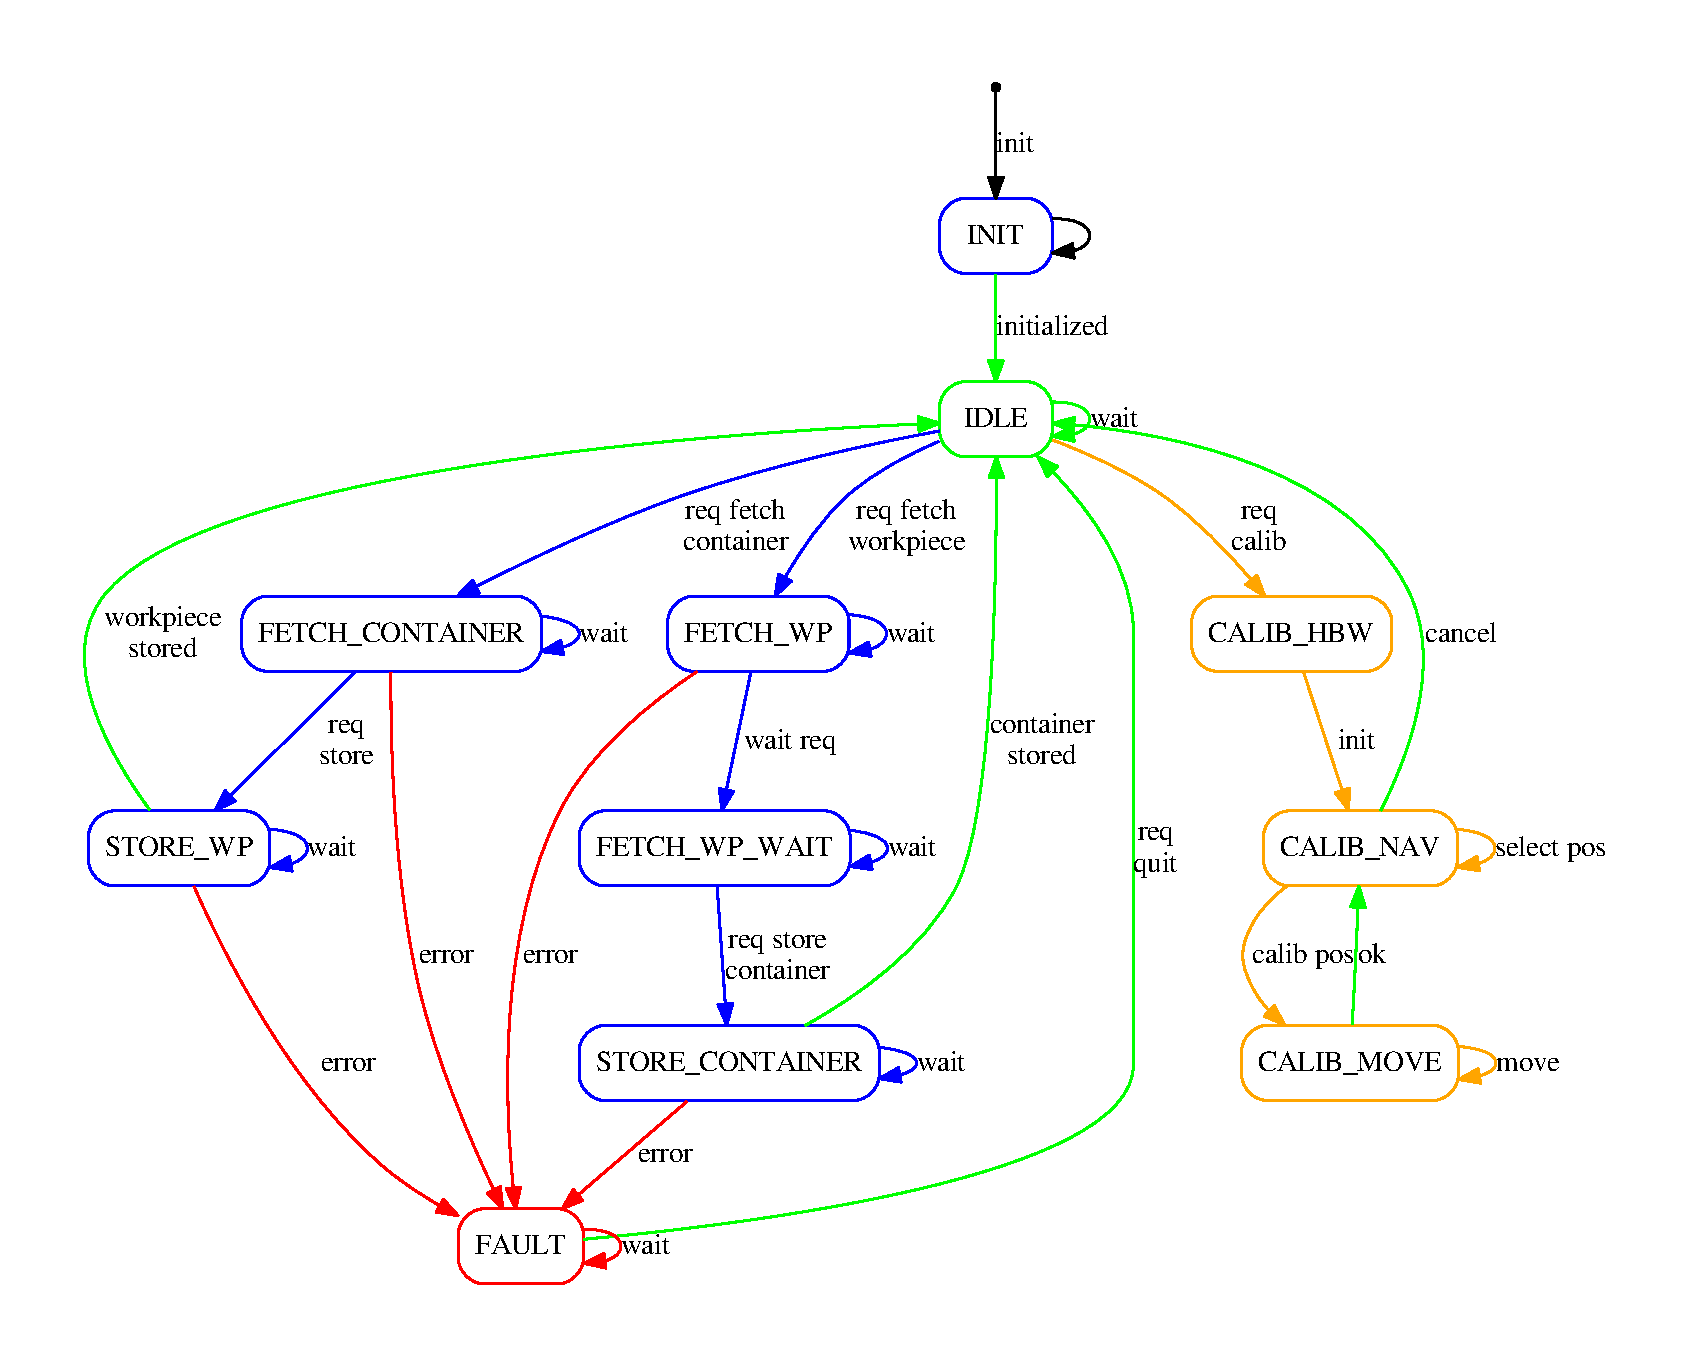
\includegraphics[width=\textwidth,height=\textheight/2,keepaspectratio=true]{dot_TxtHighBayWarehouseRun}}
\end{DoxyImageNoCaption}
 

Implements \hyperlink{classft_1_1_txt_simulation_model_a91595c8fc91104e98d2ea13fe349b777}{ft\+::\+Txt\+Simulation\+Model}.

\index{ft\+::\+Txt\+High\+Bay\+Warehouse@{ft\+::\+Txt\+High\+Bay\+Warehouse}!save\+Calib\+Default@{save\+Calib\+Default}}
\index{save\+Calib\+Default@{save\+Calib\+Default}!ft\+::\+Txt\+High\+Bay\+Warehouse@{ft\+::\+Txt\+High\+Bay\+Warehouse}}
\subsubsection[{\texorpdfstring{save\+Calib\+Default()}{saveCalibDefault()}}]{\setlength{\rightskip}{0pt plus 5cm}bool ft\+::\+Txt\+High\+Bay\+Warehouse\+::save\+Calib\+Default (
\begin{DoxyParamCaption}
{}
\end{DoxyParamCaption}
)}\hypertarget{classft_1_1_txt_high_bay_warehouse_ae6deca6a80680d0d563fde5296b618cb}{}\label{classft_1_1_txt_high_bay_warehouse_ae6deca6a80680d0d563fde5296b618cb}
\index{ft\+::\+Txt\+High\+Bay\+Warehouse@{ft\+::\+Txt\+High\+Bay\+Warehouse}!set\+Speed@{set\+Speed}}
\index{set\+Speed@{set\+Speed}!ft\+::\+Txt\+High\+Bay\+Warehouse@{ft\+::\+Txt\+High\+Bay\+Warehouse}}
\subsubsection[{\texorpdfstring{set\+Speed(int16\+\_\+t s)}{setSpeed(int16_t s)}}]{\setlength{\rightskip}{0pt plus 5cm}void ft\+::\+Txt\+High\+Bay\+Warehouse\+::set\+Speed (
\begin{DoxyParamCaption}
\item[{int16\+\_\+t}]{s}
\end{DoxyParamCaption}
)}\hypertarget{classft_1_1_txt_high_bay_warehouse_ad8900c4005609dde97e2162ef9f72031}{}\label{classft_1_1_txt_high_bay_warehouse_ad8900c4005609dde97e2162ef9f72031}
\index{ft\+::\+Txt\+High\+Bay\+Warehouse@{ft\+::\+Txt\+High\+Bay\+Warehouse}!stop@{stop}}
\index{stop@{stop}!ft\+::\+Txt\+High\+Bay\+Warehouse@{ft\+::\+Txt\+High\+Bay\+Warehouse}}
\subsubsection[{\texorpdfstring{stop()}{stop()}}]{\setlength{\rightskip}{0pt plus 5cm}void ft\+::\+Txt\+High\+Bay\+Warehouse\+::stop (
\begin{DoxyParamCaption}
{}
\end{DoxyParamCaption}
)}\hypertarget{classft_1_1_txt_high_bay_warehouse_a486b766d3f8f11a023daee496429faf0}{}\label{classft_1_1_txt_high_bay_warehouse_a486b766d3f8f11a023daee496429faf0}
\index{ft\+::\+Txt\+High\+Bay\+Warehouse@{ft\+::\+Txt\+High\+Bay\+Warehouse}!store@{store}}
\index{store@{store}!ft\+::\+Txt\+High\+Bay\+Warehouse@{ft\+::\+Txt\+High\+Bay\+Warehouse}}
\subsubsection[{\texorpdfstring{store(\+Txt\+Workpiece wp)}{store(TxtWorkpiece wp)}}]{\setlength{\rightskip}{0pt plus 5cm}bool ft\+::\+Txt\+High\+Bay\+Warehouse\+::store (
\begin{DoxyParamCaption}
\item[{{\bf Txt\+Workpiece}}]{wp}
\end{DoxyParamCaption}
)}\hypertarget{classft_1_1_txt_high_bay_warehouse_afed1cdc629d97c3776acd48fbc737780}{}\label{classft_1_1_txt_high_bay_warehouse_afed1cdc629d97c3776acd48fbc737780}
\index{ft\+::\+Txt\+High\+Bay\+Warehouse@{ft\+::\+Txt\+High\+Bay\+Warehouse}!store\+Container@{store\+Container}}
\index{store\+Container@{store\+Container}!ft\+::\+Txt\+High\+Bay\+Warehouse@{ft\+::\+Txt\+High\+Bay\+Warehouse}}
\subsubsection[{\texorpdfstring{store\+Container()}{storeContainer()}}]{\setlength{\rightskip}{0pt plus 5cm}bool ft\+::\+Txt\+High\+Bay\+Warehouse\+::store\+Container (
\begin{DoxyParamCaption}
{}
\end{DoxyParamCaption}
)}\hypertarget{classft_1_1_txt_high_bay_warehouse_adf0ee6b1f8ef44a317fb360de6ad0cc6}{}\label{classft_1_1_txt_high_bay_warehouse_adf0ee6b1f8ef44a317fb360de6ad0cc6}
\index{ft\+::\+Txt\+High\+Bay\+Warehouse@{ft\+::\+Txt\+High\+Bay\+Warehouse}!to\+String@{to\+String}}
\index{to\+String@{to\+String}!ft\+::\+Txt\+High\+Bay\+Warehouse@{ft\+::\+Txt\+High\+Bay\+Warehouse}}
\subsubsection[{\texorpdfstring{to\+String(\+State\+\_\+t state)}{toString(State_t state)}}]{\setlength{\rightskip}{0pt plus 5cm}const char$\ast$ ft\+::\+Txt\+High\+Bay\+Warehouse\+::to\+String (
\begin{DoxyParamCaption}
\item[{{\bf State\+\_\+t}}]{state}
\end{DoxyParamCaption}
)\hspace{0.3cm}{\ttfamily [inline]}}\hypertarget{classft_1_1_txt_high_bay_warehouse_abeb6f6eb81f6f14ebb9040c160acc625}{}\label{classft_1_1_txt_high_bay_warehouse_abeb6f6eb81f6f14ebb9040c160acc625}


\subsection{Friends And Related Function Documentation}
\index{ft\+::\+Txt\+High\+Bay\+Warehouse@{ft\+::\+Txt\+High\+Bay\+Warehouse}!Txt\+Joystick\+X\+Y\+B\+Controller@{Txt\+Joystick\+X\+Y\+B\+Controller}}
\index{Txt\+Joystick\+X\+Y\+B\+Controller@{Txt\+Joystick\+X\+Y\+B\+Controller}!ft\+::\+Txt\+High\+Bay\+Warehouse@{ft\+::\+Txt\+High\+Bay\+Warehouse}}
\subsubsection[{\texorpdfstring{Txt\+Joystick\+X\+Y\+B\+Controller}{TxtJoystickXYBController}}]{\setlength{\rightskip}{0pt plus 5cm}friend class {\bf Txt\+Joystick\+X\+Y\+B\+Controller}\hspace{0.3cm}{\ttfamily [friend]}}\hypertarget{classft_1_1_txt_high_bay_warehouse_a23c350af40fe2a0866b409315c4dfe1a}{}\label{classft_1_1_txt_high_bay_warehouse_a23c350af40fe2a0866b409315c4dfe1a}


\subsection{Member Data Documentation}
\index{ft\+::\+Txt\+High\+Bay\+Warehouse@{ft\+::\+Txt\+High\+Bay\+Warehouse}!axisX@{axisX}}
\index{axisX@{axisX}!ft\+::\+Txt\+High\+Bay\+Warehouse@{ft\+::\+Txt\+High\+Bay\+Warehouse}}
\subsubsection[{\texorpdfstring{axisX}{axisX}}]{\setlength{\rightskip}{0pt plus 5cm}{\bf Txt\+Axis1\+Ref\+Switch} ft\+::\+Txt\+High\+Bay\+Warehouse\+::axisX\hspace{0.3cm}{\ttfamily [protected]}}\hypertarget{classft_1_1_txt_high_bay_warehouse_a32aff14ae3169fe5f4b94268362ab757}{}\label{classft_1_1_txt_high_bay_warehouse_a32aff14ae3169fe5f4b94268362ab757}
\index{ft\+::\+Txt\+High\+Bay\+Warehouse@{ft\+::\+Txt\+High\+Bay\+Warehouse}!axisY@{axisY}}
\index{axisY@{axisY}!ft\+::\+Txt\+High\+Bay\+Warehouse@{ft\+::\+Txt\+High\+Bay\+Warehouse}}
\subsubsection[{\texorpdfstring{axisY}{axisY}}]{\setlength{\rightskip}{0pt plus 5cm}{\bf Txt\+Axis1\+Ref\+Switch} ft\+::\+Txt\+High\+Bay\+Warehouse\+::axisY\hspace{0.3cm}{\ttfamily [protected]}}\hypertarget{classft_1_1_txt_high_bay_warehouse_a5e65f43da4467849a5c45e0e8ec109c5}{}\label{classft_1_1_txt_high_bay_warehouse_a5e65f43da4467849a5c45e0e8ec109c5}
\index{ft\+::\+Txt\+High\+Bay\+Warehouse@{ft\+::\+Txt\+High\+Bay\+Warehouse}!axisZ@{axisZ}}
\index{axisZ@{axisZ}!ft\+::\+Txt\+High\+Bay\+Warehouse@{ft\+::\+Txt\+High\+Bay\+Warehouse}}
\subsubsection[{\texorpdfstring{axisZ}{axisZ}}]{\setlength{\rightskip}{0pt plus 5cm}{\bf Txt\+Axis\+N\+Ref\+Switch} ft\+::\+Txt\+High\+Bay\+Warehouse\+::axisZ\hspace{0.3cm}{\ttfamily [protected]}}\hypertarget{classft_1_1_txt_high_bay_warehouse_a8df26228e9b0a93fb4cd9301661841fc}{}\label{classft_1_1_txt_high_bay_warehouse_a8df26228e9b0a93fb4cd9301661841fc}
\index{ft\+::\+Txt\+High\+Bay\+Warehouse@{ft\+::\+Txt\+High\+Bay\+Warehouse}!calib\+Data@{calib\+Data}}
\index{calib\+Data@{calib\+Data}!ft\+::\+Txt\+High\+Bay\+Warehouse@{ft\+::\+Txt\+High\+Bay\+Warehouse}}
\subsubsection[{\texorpdfstring{calib\+Data}{calibData}}]{\setlength{\rightskip}{0pt plus 5cm}{\bf Txt\+High\+Bay\+Warehouse\+Calib\+Data} ft\+::\+Txt\+High\+Bay\+Warehouse\+::calib\+Data\hspace{0.3cm}{\ttfamily [protected]}}\hypertarget{classft_1_1_txt_high_bay_warehouse_a6f59992878b73195da5a64ba7cec19ac}{}\label{classft_1_1_txt_high_bay_warehouse_a6f59992878b73195da5a64ba7cec19ac}
\index{ft\+::\+Txt\+High\+Bay\+Warehouse@{ft\+::\+Txt\+High\+Bay\+Warehouse}!calib\+Pos@{calib\+Pos}}
\index{calib\+Pos@{calib\+Pos}!ft\+::\+Txt\+High\+Bay\+Warehouse@{ft\+::\+Txt\+High\+Bay\+Warehouse}}
\subsubsection[{\texorpdfstring{calib\+Pos}{calibPos}}]{\setlength{\rightskip}{0pt plus 5cm}{\bf Txt\+Hbw\+Calib\+Pos\+\_\+t} ft\+::\+Txt\+High\+Bay\+Warehouse\+::calib\+Pos\hspace{0.3cm}{\ttfamily [protected]}}\hypertarget{classft_1_1_txt_high_bay_warehouse_a4efec14e60a1c700524d0f37599df4a7}{}\label{classft_1_1_txt_high_bay_warehouse_a4efec14e60a1c700524d0f37599df4a7}
\index{ft\+::\+Txt\+High\+Bay\+Warehouse@{ft\+::\+Txt\+High\+Bay\+Warehouse}!conv\+Belt@{conv\+Belt}}
\index{conv\+Belt@{conv\+Belt}!ft\+::\+Txt\+High\+Bay\+Warehouse@{ft\+::\+Txt\+High\+Bay\+Warehouse}}
\subsubsection[{\texorpdfstring{conv\+Belt}{convBelt}}]{\setlength{\rightskip}{0pt plus 5cm}{\bf Txt\+Conveyor\+Belt\+Light\+Barriers} ft\+::\+Txt\+High\+Bay\+Warehouse\+::conv\+Belt\hspace{0.3cm}{\ttfamily [protected]}}\hypertarget{classft_1_1_txt_high_bay_warehouse_a21a7a8b3f7f7bd8b8d9b375f956e043d}{}\label{classft_1_1_txt_high_bay_warehouse_a21a7a8b3f7f7bd8b8d9b375f956e043d}
\index{ft\+::\+Txt\+High\+Bay\+Warehouse@{ft\+::\+Txt\+High\+Bay\+Warehouse}!current\+State@{current\+State}}
\index{current\+State@{current\+State}!ft\+::\+Txt\+High\+Bay\+Warehouse@{ft\+::\+Txt\+High\+Bay\+Warehouse}}
\subsubsection[{\texorpdfstring{current\+State}{currentState}}]{\setlength{\rightskip}{0pt plus 5cm}{\bf State\+\_\+t} ft\+::\+Txt\+High\+Bay\+Warehouse\+::current\+State\hspace{0.3cm}{\ttfamily [protected]}}\hypertarget{classft_1_1_txt_high_bay_warehouse_a15a6bfc9bbc73841e4deb8e5957ed76c}{}\label{classft_1_1_txt_high_bay_warehouse_a15a6bfc9bbc73841e4deb8e5957ed76c}
\index{ft\+::\+Txt\+High\+Bay\+Warehouse@{ft\+::\+Txt\+High\+Bay\+Warehouse}!joy\+Data@{joy\+Data}}
\index{joy\+Data@{joy\+Data}!ft\+::\+Txt\+High\+Bay\+Warehouse@{ft\+::\+Txt\+High\+Bay\+Warehouse}}
\subsubsection[{\texorpdfstring{joy\+Data}{joyData}}]{\setlength{\rightskip}{0pt plus 5cm}{\bf Txt\+Joysticks\+Data} ft\+::\+Txt\+High\+Bay\+Warehouse\+::joy\+Data\hspace{0.3cm}{\ttfamily [protected]}}\hypertarget{classft_1_1_txt_high_bay_warehouse_a9198fb21f8df14c39a42918c8f7fb229}{}\label{classft_1_1_txt_high_bay_warehouse_a9198fb21f8df14c39a42918c8f7fb229}
\index{ft\+::\+Txt\+High\+Bay\+Warehouse@{ft\+::\+Txt\+High\+Bay\+Warehouse}!last\+Pos2@{last\+Pos2}}
\index{last\+Pos2@{last\+Pos2}!ft\+::\+Txt\+High\+Bay\+Warehouse@{ft\+::\+Txt\+High\+Bay\+Warehouse}}
\subsubsection[{\texorpdfstring{last\+Pos2}{lastPos2}}]{\setlength{\rightskip}{0pt plus 5cm}{\bf Enc\+Pos2} ft\+::\+Txt\+High\+Bay\+Warehouse\+::last\+Pos2\hspace{0.3cm}{\ttfamily [protected]}}\hypertarget{classft_1_1_txt_high_bay_warehouse_adff0e6e55befd942c89e1ae10e5fb910}{}\label{classft_1_1_txt_high_bay_warehouse_adff0e6e55befd942c89e1ae10e5fb910}
\index{ft\+::\+Txt\+High\+Bay\+Warehouse@{ft\+::\+Txt\+High\+Bay\+Warehouse}!new\+State@{new\+State}}
\index{new\+State@{new\+State}!ft\+::\+Txt\+High\+Bay\+Warehouse@{ft\+::\+Txt\+High\+Bay\+Warehouse}}
\subsubsection[{\texorpdfstring{new\+State}{newState}}]{\setlength{\rightskip}{0pt plus 5cm}{\bf State\+\_\+t} ft\+::\+Txt\+High\+Bay\+Warehouse\+::new\+State\hspace{0.3cm}{\ttfamily [protected]}}\hypertarget{classft_1_1_txt_high_bay_warehouse_a5c034252f7f1477ccb0acc21148c6d4c}{}\label{classft_1_1_txt_high_bay_warehouse_a5c034252f7f1477ccb0acc21148c6d4c}
\index{ft\+::\+Txt\+High\+Bay\+Warehouse@{ft\+::\+Txt\+High\+Bay\+Warehouse}!obs\+\_\+hbw@{obs\+\_\+hbw}}
\index{obs\+\_\+hbw@{obs\+\_\+hbw}!ft\+::\+Txt\+High\+Bay\+Warehouse@{ft\+::\+Txt\+High\+Bay\+Warehouse}}
\subsubsection[{\texorpdfstring{obs\+\_\+hbw}{obs_hbw}}]{\setlength{\rightskip}{0pt plus 5cm}{\bf Txt\+High\+Bay\+Warehouse\+Observer}$\ast$ ft\+::\+Txt\+High\+Bay\+Warehouse\+::obs\+\_\+hbw\hspace{0.3cm}{\ttfamily [protected]}}\hypertarget{classft_1_1_txt_high_bay_warehouse_abea430ced2afa416b2abaaea7b79ad43}{}\label{classft_1_1_txt_high_bay_warehouse_abea430ced2afa416b2abaaea7b79ad43}
\index{ft\+::\+Txt\+High\+Bay\+Warehouse@{ft\+::\+Txt\+High\+Bay\+Warehouse}!obs\+\_\+storage@{obs\+\_\+storage}}
\index{obs\+\_\+storage@{obs\+\_\+storage}!ft\+::\+Txt\+High\+Bay\+Warehouse@{ft\+::\+Txt\+High\+Bay\+Warehouse}}
\subsubsection[{\texorpdfstring{obs\+\_\+storage}{obs_storage}}]{\setlength{\rightskip}{0pt plus 5cm}{\bf Txt\+High\+Bay\+Warehouse\+Storage\+Observer}$\ast$ ft\+::\+Txt\+High\+Bay\+Warehouse\+::obs\+\_\+storage\hspace{0.3cm}{\ttfamily [protected]}}\hypertarget{classft_1_1_txt_high_bay_warehouse_af041aca8d94f924075cae8c7edb2eda2}{}\label{classft_1_1_txt_high_bay_warehouse_af041aca8d94f924075cae8c7edb2eda2}
\index{ft\+::\+Txt\+High\+Bay\+Warehouse@{ft\+::\+Txt\+High\+Bay\+Warehouse}!req\+Joy\+Data@{req\+Joy\+Data}}
\index{req\+Joy\+Data@{req\+Joy\+Data}!ft\+::\+Txt\+High\+Bay\+Warehouse@{ft\+::\+Txt\+High\+Bay\+Warehouse}}
\subsubsection[{\texorpdfstring{req\+Joy\+Data}{reqJoyData}}]{\setlength{\rightskip}{0pt plus 5cm}bool ft\+::\+Txt\+High\+Bay\+Warehouse\+::req\+Joy\+Data\hspace{0.3cm}{\ttfamily [protected]}}\hypertarget{classft_1_1_txt_high_bay_warehouse_a012b13872f28ba32973d0f4f8459243d}{}\label{classft_1_1_txt_high_bay_warehouse_a012b13872f28ba32973d0f4f8459243d}
\index{ft\+::\+Txt\+High\+Bay\+Warehouse@{ft\+::\+Txt\+High\+Bay\+Warehouse}!req\+Quit@{req\+Quit}}
\index{req\+Quit@{req\+Quit}!ft\+::\+Txt\+High\+Bay\+Warehouse@{ft\+::\+Txt\+High\+Bay\+Warehouse}}
\subsubsection[{\texorpdfstring{req\+Quit}{reqQuit}}]{\setlength{\rightskip}{0pt plus 5cm}bool ft\+::\+Txt\+High\+Bay\+Warehouse\+::req\+Quit\hspace{0.3cm}{\ttfamily [protected]}}\hypertarget{classft_1_1_txt_high_bay_warehouse_abb655a59ffddd97aa2e009e328309a5c}{}\label{classft_1_1_txt_high_bay_warehouse_abb655a59ffddd97aa2e009e328309a5c}
\index{ft\+::\+Txt\+High\+Bay\+Warehouse@{ft\+::\+Txt\+High\+Bay\+Warehouse}!req\+V\+G\+Rcalib@{req\+V\+G\+Rcalib}}
\index{req\+V\+G\+Rcalib@{req\+V\+G\+Rcalib}!ft\+::\+Txt\+High\+Bay\+Warehouse@{ft\+::\+Txt\+High\+Bay\+Warehouse}}
\subsubsection[{\texorpdfstring{req\+V\+G\+Rcalib}{reqVGRcalib}}]{\setlength{\rightskip}{0pt plus 5cm}bool ft\+::\+Txt\+High\+Bay\+Warehouse\+::req\+V\+G\+Rcalib\hspace{0.3cm}{\ttfamily [protected]}}\hypertarget{classft_1_1_txt_high_bay_warehouse_a9dbb34e1a49f2835e07966fdb352f693}{}\label{classft_1_1_txt_high_bay_warehouse_a9dbb34e1a49f2835e07966fdb352f693}
\index{ft\+::\+Txt\+High\+Bay\+Warehouse@{ft\+::\+Txt\+High\+Bay\+Warehouse}!req\+V\+G\+Rfetch@{req\+V\+G\+Rfetch}}
\index{req\+V\+G\+Rfetch@{req\+V\+G\+Rfetch}!ft\+::\+Txt\+High\+Bay\+Warehouse@{ft\+::\+Txt\+High\+Bay\+Warehouse}}
\subsubsection[{\texorpdfstring{req\+V\+G\+Rfetch}{reqVGRfetch}}]{\setlength{\rightskip}{0pt plus 5cm}bool ft\+::\+Txt\+High\+Bay\+Warehouse\+::req\+V\+G\+Rfetch\hspace{0.3cm}{\ttfamily [protected]}}\hypertarget{classft_1_1_txt_high_bay_warehouse_a90e4e190386d912fb068bcc5bf033fd4}{}\label{classft_1_1_txt_high_bay_warehouse_a90e4e190386d912fb068bcc5bf033fd4}
\index{ft\+::\+Txt\+High\+Bay\+Warehouse@{ft\+::\+Txt\+High\+Bay\+Warehouse}!req\+V\+G\+Rfetch\+Container@{req\+V\+G\+Rfetch\+Container}}
\index{req\+V\+G\+Rfetch\+Container@{req\+V\+G\+Rfetch\+Container}!ft\+::\+Txt\+High\+Bay\+Warehouse@{ft\+::\+Txt\+High\+Bay\+Warehouse}}
\subsubsection[{\texorpdfstring{req\+V\+G\+Rfetch\+Container}{reqVGRfetchContainer}}]{\setlength{\rightskip}{0pt plus 5cm}bool ft\+::\+Txt\+High\+Bay\+Warehouse\+::req\+V\+G\+Rfetch\+Container\hspace{0.3cm}{\ttfamily [protected]}}\hypertarget{classft_1_1_txt_high_bay_warehouse_a837761587b4c7873a28b757aa660f463}{}\label{classft_1_1_txt_high_bay_warehouse_a837761587b4c7873a28b757aa660f463}
\index{ft\+::\+Txt\+High\+Bay\+Warehouse@{ft\+::\+Txt\+High\+Bay\+Warehouse}!req\+V\+G\+Rreset\+Storage@{req\+V\+G\+Rreset\+Storage}}
\index{req\+V\+G\+Rreset\+Storage@{req\+V\+G\+Rreset\+Storage}!ft\+::\+Txt\+High\+Bay\+Warehouse@{ft\+::\+Txt\+High\+Bay\+Warehouse}}
\subsubsection[{\texorpdfstring{req\+V\+G\+Rreset\+Storage}{reqVGRresetStorage}}]{\setlength{\rightskip}{0pt plus 5cm}bool ft\+::\+Txt\+High\+Bay\+Warehouse\+::req\+V\+G\+Rreset\+Storage\hspace{0.3cm}{\ttfamily [protected]}}\hypertarget{classft_1_1_txt_high_bay_warehouse_abe22fa14074fcc26c56aef48a6ffec0a}{}\label{classft_1_1_txt_high_bay_warehouse_abe22fa14074fcc26c56aef48a6ffec0a}
\index{ft\+::\+Txt\+High\+Bay\+Warehouse@{ft\+::\+Txt\+High\+Bay\+Warehouse}!req\+V\+G\+Rstore@{req\+V\+G\+Rstore}}
\index{req\+V\+G\+Rstore@{req\+V\+G\+Rstore}!ft\+::\+Txt\+High\+Bay\+Warehouse@{ft\+::\+Txt\+High\+Bay\+Warehouse}}
\subsubsection[{\texorpdfstring{req\+V\+G\+Rstore}{reqVGRstore}}]{\setlength{\rightskip}{0pt plus 5cm}bool ft\+::\+Txt\+High\+Bay\+Warehouse\+::req\+V\+G\+Rstore\hspace{0.3cm}{\ttfamily [protected]}}\hypertarget{classft_1_1_txt_high_bay_warehouse_a2cf5cf9e6dd1cdf57a9082161798fbca}{}\label{classft_1_1_txt_high_bay_warehouse_a2cf5cf9e6dd1cdf57a9082161798fbca}
\index{ft\+::\+Txt\+High\+Bay\+Warehouse@{ft\+::\+Txt\+High\+Bay\+Warehouse}!req\+V\+G\+Rstore\+Container@{req\+V\+G\+Rstore\+Container}}
\index{req\+V\+G\+Rstore\+Container@{req\+V\+G\+Rstore\+Container}!ft\+::\+Txt\+High\+Bay\+Warehouse@{ft\+::\+Txt\+High\+Bay\+Warehouse}}
\subsubsection[{\texorpdfstring{req\+V\+G\+Rstore\+Container}{reqVGRstoreContainer}}]{\setlength{\rightskip}{0pt plus 5cm}bool ft\+::\+Txt\+High\+Bay\+Warehouse\+::req\+V\+G\+Rstore\+Container\hspace{0.3cm}{\ttfamily [protected]}}\hypertarget{classft_1_1_txt_high_bay_warehouse_a34b88b73e4a10815a453debc756d8d0b}{}\label{classft_1_1_txt_high_bay_warehouse_a34b88b73e4a10815a453debc756d8d0b}
\index{ft\+::\+Txt\+High\+Bay\+Warehouse@{ft\+::\+Txt\+High\+Bay\+Warehouse}!req\+V\+G\+Rwp@{req\+V\+G\+Rwp}}
\index{req\+V\+G\+Rwp@{req\+V\+G\+Rwp}!ft\+::\+Txt\+High\+Bay\+Warehouse@{ft\+::\+Txt\+High\+Bay\+Warehouse}}
\subsubsection[{\texorpdfstring{req\+V\+G\+Rwp}{reqVGRwp}}]{\setlength{\rightskip}{0pt plus 5cm}{\bf Txt\+Workpiece}$\ast$ ft\+::\+Txt\+High\+Bay\+Warehouse\+::req\+V\+G\+Rwp\hspace{0.3cm}{\ttfamily [protected]}}\hypertarget{classft_1_1_txt_high_bay_warehouse_a75ccda2cc4ff08480f6b5d886e35d867}{}\label{classft_1_1_txt_high_bay_warehouse_a75ccda2cc4ff08480f6b5d886e35d867}
\index{ft\+::\+Txt\+High\+Bay\+Warehouse@{ft\+::\+Txt\+High\+Bay\+Warehouse}!storage@{storage}}
\index{storage@{storage}!ft\+::\+Txt\+High\+Bay\+Warehouse@{ft\+::\+Txt\+High\+Bay\+Warehouse}}
\subsubsection[{\texorpdfstring{storage}{storage}}]{\setlength{\rightskip}{0pt plus 5cm}{\bf Txt\+High\+Bay\+Warehouse\+Storage} ft\+::\+Txt\+High\+Bay\+Warehouse\+::storage\hspace{0.3cm}{\ttfamily [protected]}}\hypertarget{classft_1_1_txt_high_bay_warehouse_af7b1534ad416b0f0f86c2792e2982a4f}{}\label{classft_1_1_txt_high_bay_warehouse_af7b1534ad416b0f0f86c2792e2982a4f}
\index{ft\+::\+Txt\+High\+Bay\+Warehouse@{ft\+::\+Txt\+High\+Bay\+Warehouse}!ydelta@{ydelta}}
\index{ydelta@{ydelta}!ft\+::\+Txt\+High\+Bay\+Warehouse@{ft\+::\+Txt\+High\+Bay\+Warehouse}}
\subsubsection[{\texorpdfstring{ydelta}{ydelta}}]{\setlength{\rightskip}{0pt plus 5cm}const int ft\+::\+Txt\+High\+Bay\+Warehouse\+::ydelta = 40}\hypertarget{classft_1_1_txt_high_bay_warehouse_acfdcf3b84851e9315c7e243c8fbda76d}{}\label{classft_1_1_txt_high_bay_warehouse_acfdcf3b84851e9315c7e243c8fbda76d}


The documentation for this class was generated from the following file\+:\begin{DoxyCompactItemize}
\item 
\hyperlink{_txt_high_bay_warehouse_8h}{Txt\+High\+Bay\+Warehouse.\+h}\end{DoxyCompactItemize}

\hypertarget{classft_1_1_txt_high_bay_warehouse_calib_data}{}\section{ft\+:\+:Txt\+High\+Bay\+Warehouse\+Calib\+Data Class Reference}
\label{classft_1_1_txt_high_bay_warehouse_calib_data}\index{ft\+::\+Txt\+High\+Bay\+Warehouse\+Calib\+Data@{ft\+::\+Txt\+High\+Bay\+Warehouse\+Calib\+Data}}


{\ttfamily \#include $<$Txt\+High\+Bay\+Warehouse.\+h$>$}



Inheritance diagram for ft\+:\+:Txt\+High\+Bay\+Warehouse\+Calib\+Data\+:
\nopagebreak
\begin{figure}[H]
\begin{center}
\leavevmode
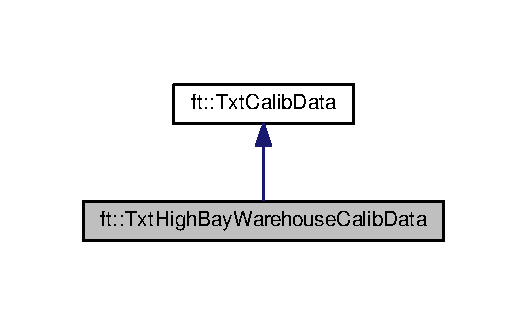
\includegraphics[width=253pt]{classft_1_1_txt_high_bay_warehouse_calib_data__inherit__graph}
\end{center}
\end{figure}


Collaboration diagram for ft\+:\+:Txt\+High\+Bay\+Warehouse\+Calib\+Data\+:
\nopagebreak
\begin{figure}[H]
\begin{center}
\leavevmode
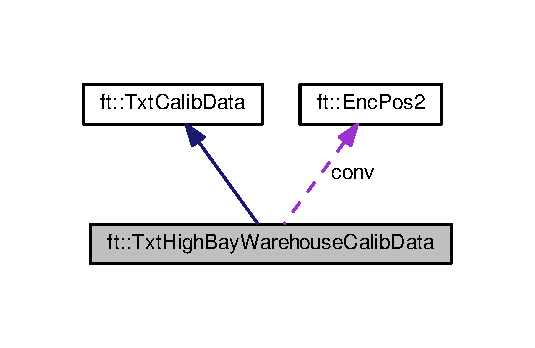
\includegraphics[width=257pt]{classft_1_1_txt_high_bay_warehouse_calib_data__coll__graph}
\end{center}
\end{figure}
\subsection*{Public Member Functions}
\begin{DoxyCompactItemize}
\item 
\hyperlink{classft_1_1_txt_high_bay_warehouse_calib_data_ab19ab76a04a49f0e3ce7fa4123a84470}{Txt\+High\+Bay\+Warehouse\+Calib\+Data} ()
\item 
virtual \hyperlink{classft_1_1_txt_high_bay_warehouse_calib_data_a318de726a93b922743284337526d9223}{$\sim$\+Txt\+High\+Bay\+Warehouse\+Calib\+Data} ()
\item 
bool \hyperlink{classft_1_1_txt_high_bay_warehouse_calib_data_a018f042864bebde45e9f138bff550ec9}{load} ()
\item 
bool \hyperlink{classft_1_1_txt_high_bay_warehouse_calib_data_ac8d87668f8d0347714f6545954df3573}{save\+Default} ()
\item 
bool \hyperlink{classft_1_1_txt_high_bay_warehouse_calib_data_a193721ae3de0052eb1a3b74f877363a6}{save} ()
\end{DoxyCompactItemize}
\subsection*{Public Attributes}
\begin{DoxyCompactItemize}
\item 
uint16\+\_\+t \hyperlink{classft_1_1_txt_high_bay_warehouse_calib_data_a90910cc5144915878a613a9a248ea66f}{hbx} \mbox{[}3\mbox{]}
\item 
uint16\+\_\+t \hyperlink{classft_1_1_txt_high_bay_warehouse_calib_data_a6f12021cef4ed3d547cfade44616c15f}{hby} \mbox{[}3\mbox{]}
\item 
\hyperlink{classft_1_1_enc_pos2}{Enc\+Pos2} \hyperlink{classft_1_1_txt_high_bay_warehouse_calib_data_a978a3f44d70956000e110a66b17cf36e}{conv}
\end{DoxyCompactItemize}
\subsection*{Additional Inherited Members}


\subsection{Constructor \& Destructor Documentation}
\index{ft\+::\+Txt\+High\+Bay\+Warehouse\+Calib\+Data@{ft\+::\+Txt\+High\+Bay\+Warehouse\+Calib\+Data}!Txt\+High\+Bay\+Warehouse\+Calib\+Data@{Txt\+High\+Bay\+Warehouse\+Calib\+Data}}
\index{Txt\+High\+Bay\+Warehouse\+Calib\+Data@{Txt\+High\+Bay\+Warehouse\+Calib\+Data}!ft\+::\+Txt\+High\+Bay\+Warehouse\+Calib\+Data@{ft\+::\+Txt\+High\+Bay\+Warehouse\+Calib\+Data}}
\subsubsection[{\texorpdfstring{Txt\+High\+Bay\+Warehouse\+Calib\+Data()}{TxtHighBayWarehouseCalibData()}}]{\setlength{\rightskip}{0pt plus 5cm}ft\+::\+Txt\+High\+Bay\+Warehouse\+Calib\+Data\+::\+Txt\+High\+Bay\+Warehouse\+Calib\+Data (
\begin{DoxyParamCaption}
{}
\end{DoxyParamCaption}
)\hspace{0.3cm}{\ttfamily [inline]}}\hypertarget{classft_1_1_txt_high_bay_warehouse_calib_data_ab19ab76a04a49f0e3ce7fa4123a84470}{}\label{classft_1_1_txt_high_bay_warehouse_calib_data_ab19ab76a04a49f0e3ce7fa4123a84470}
\index{ft\+::\+Txt\+High\+Bay\+Warehouse\+Calib\+Data@{ft\+::\+Txt\+High\+Bay\+Warehouse\+Calib\+Data}!````~Txt\+High\+Bay\+Warehouse\+Calib\+Data@{$\sim$\+Txt\+High\+Bay\+Warehouse\+Calib\+Data}}
\index{````~Txt\+High\+Bay\+Warehouse\+Calib\+Data@{$\sim$\+Txt\+High\+Bay\+Warehouse\+Calib\+Data}!ft\+::\+Txt\+High\+Bay\+Warehouse\+Calib\+Data@{ft\+::\+Txt\+High\+Bay\+Warehouse\+Calib\+Data}}
\subsubsection[{\texorpdfstring{$\sim$\+Txt\+High\+Bay\+Warehouse\+Calib\+Data()}{~TxtHighBayWarehouseCalibData()}}]{\setlength{\rightskip}{0pt plus 5cm}virtual ft\+::\+Txt\+High\+Bay\+Warehouse\+Calib\+Data\+::$\sim$\+Txt\+High\+Bay\+Warehouse\+Calib\+Data (
\begin{DoxyParamCaption}
{}
\end{DoxyParamCaption}
)\hspace{0.3cm}{\ttfamily [inline]}, {\ttfamily [virtual]}}\hypertarget{classft_1_1_txt_high_bay_warehouse_calib_data_a318de726a93b922743284337526d9223}{}\label{classft_1_1_txt_high_bay_warehouse_calib_data_a318de726a93b922743284337526d9223}


\subsection{Member Function Documentation}
\index{ft\+::\+Txt\+High\+Bay\+Warehouse\+Calib\+Data@{ft\+::\+Txt\+High\+Bay\+Warehouse\+Calib\+Data}!load@{load}}
\index{load@{load}!ft\+::\+Txt\+High\+Bay\+Warehouse\+Calib\+Data@{ft\+::\+Txt\+High\+Bay\+Warehouse\+Calib\+Data}}
\subsubsection[{\texorpdfstring{load()}{load()}}]{\setlength{\rightskip}{0pt plus 5cm}bool ft\+::\+Txt\+High\+Bay\+Warehouse\+Calib\+Data\+::load (
\begin{DoxyParamCaption}
{}
\end{DoxyParamCaption}
)\hspace{0.3cm}{\ttfamily [virtual]}}\hypertarget{classft_1_1_txt_high_bay_warehouse_calib_data_a018f042864bebde45e9f138bff550ec9}{}\label{classft_1_1_txt_high_bay_warehouse_calib_data_a018f042864bebde45e9f138bff550ec9}


Implements \hyperlink{classft_1_1_txt_calib_data_abe888396c95ead8fd554fc77ba486e7a}{ft\+::\+Txt\+Calib\+Data}.

\index{ft\+::\+Txt\+High\+Bay\+Warehouse\+Calib\+Data@{ft\+::\+Txt\+High\+Bay\+Warehouse\+Calib\+Data}!save@{save}}
\index{save@{save}!ft\+::\+Txt\+High\+Bay\+Warehouse\+Calib\+Data@{ft\+::\+Txt\+High\+Bay\+Warehouse\+Calib\+Data}}
\subsubsection[{\texorpdfstring{save()}{save()}}]{\setlength{\rightskip}{0pt plus 5cm}bool ft\+::\+Txt\+High\+Bay\+Warehouse\+Calib\+Data\+::save (
\begin{DoxyParamCaption}
{}
\end{DoxyParamCaption}
)\hspace{0.3cm}{\ttfamily [virtual]}}\hypertarget{classft_1_1_txt_high_bay_warehouse_calib_data_a193721ae3de0052eb1a3b74f877363a6}{}\label{classft_1_1_txt_high_bay_warehouse_calib_data_a193721ae3de0052eb1a3b74f877363a6}


Implements \hyperlink{classft_1_1_txt_calib_data_a68a7bd5bfc32ebf82dd1a4fbe086a1b3}{ft\+::\+Txt\+Calib\+Data}.

\index{ft\+::\+Txt\+High\+Bay\+Warehouse\+Calib\+Data@{ft\+::\+Txt\+High\+Bay\+Warehouse\+Calib\+Data}!save\+Default@{save\+Default}}
\index{save\+Default@{save\+Default}!ft\+::\+Txt\+High\+Bay\+Warehouse\+Calib\+Data@{ft\+::\+Txt\+High\+Bay\+Warehouse\+Calib\+Data}}
\subsubsection[{\texorpdfstring{save\+Default()}{saveDefault()}}]{\setlength{\rightskip}{0pt plus 5cm}bool ft\+::\+Txt\+High\+Bay\+Warehouse\+Calib\+Data\+::save\+Default (
\begin{DoxyParamCaption}
{}
\end{DoxyParamCaption}
)\hspace{0.3cm}{\ttfamily [virtual]}}\hypertarget{classft_1_1_txt_high_bay_warehouse_calib_data_ac8d87668f8d0347714f6545954df3573}{}\label{classft_1_1_txt_high_bay_warehouse_calib_data_ac8d87668f8d0347714f6545954df3573}


Implements \hyperlink{classft_1_1_txt_calib_data_aace95b90ba43836acbd8f0cf1dd323c7}{ft\+::\+Txt\+Calib\+Data}.



\subsection{Member Data Documentation}
\index{ft\+::\+Txt\+High\+Bay\+Warehouse\+Calib\+Data@{ft\+::\+Txt\+High\+Bay\+Warehouse\+Calib\+Data}!conv@{conv}}
\index{conv@{conv}!ft\+::\+Txt\+High\+Bay\+Warehouse\+Calib\+Data@{ft\+::\+Txt\+High\+Bay\+Warehouse\+Calib\+Data}}
\subsubsection[{\texorpdfstring{conv}{conv}}]{\setlength{\rightskip}{0pt plus 5cm}{\bf Enc\+Pos2} ft\+::\+Txt\+High\+Bay\+Warehouse\+Calib\+Data\+::conv}\hypertarget{classft_1_1_txt_high_bay_warehouse_calib_data_a978a3f44d70956000e110a66b17cf36e}{}\label{classft_1_1_txt_high_bay_warehouse_calib_data_a978a3f44d70956000e110a66b17cf36e}
\index{ft\+::\+Txt\+High\+Bay\+Warehouse\+Calib\+Data@{ft\+::\+Txt\+High\+Bay\+Warehouse\+Calib\+Data}!hbx@{hbx}}
\index{hbx@{hbx}!ft\+::\+Txt\+High\+Bay\+Warehouse\+Calib\+Data@{ft\+::\+Txt\+High\+Bay\+Warehouse\+Calib\+Data}}
\subsubsection[{\texorpdfstring{hbx}{hbx}}]{\setlength{\rightskip}{0pt plus 5cm}uint16\+\_\+t ft\+::\+Txt\+High\+Bay\+Warehouse\+Calib\+Data\+::hbx\mbox{[}3\mbox{]}}\hypertarget{classft_1_1_txt_high_bay_warehouse_calib_data_a90910cc5144915878a613a9a248ea66f}{}\label{classft_1_1_txt_high_bay_warehouse_calib_data_a90910cc5144915878a613a9a248ea66f}
\index{ft\+::\+Txt\+High\+Bay\+Warehouse\+Calib\+Data@{ft\+::\+Txt\+High\+Bay\+Warehouse\+Calib\+Data}!hby@{hby}}
\index{hby@{hby}!ft\+::\+Txt\+High\+Bay\+Warehouse\+Calib\+Data@{ft\+::\+Txt\+High\+Bay\+Warehouse\+Calib\+Data}}
\subsubsection[{\texorpdfstring{hby}{hby}}]{\setlength{\rightskip}{0pt plus 5cm}uint16\+\_\+t ft\+::\+Txt\+High\+Bay\+Warehouse\+Calib\+Data\+::hby\mbox{[}3\mbox{]}}\hypertarget{classft_1_1_txt_high_bay_warehouse_calib_data_a6f12021cef4ed3d547cfade44616c15f}{}\label{classft_1_1_txt_high_bay_warehouse_calib_data_a6f12021cef4ed3d547cfade44616c15f}


The documentation for this class was generated from the following file\+:\begin{DoxyCompactItemize}
\item 
\hyperlink{_txt_high_bay_warehouse_8h}{Txt\+High\+Bay\+Warehouse.\+h}\end{DoxyCompactItemize}

\hypertarget{classft_1_1_txt_high_bay_warehouse_observer}{}\section{ft\+:\+:Txt\+High\+Bay\+Warehouse\+Observer Class Reference}
\label{classft_1_1_txt_high_bay_warehouse_observer}\index{ft\+::\+Txt\+High\+Bay\+Warehouse\+Observer@{ft\+::\+Txt\+High\+Bay\+Warehouse\+Observer}}


{\ttfamily \#include $<$Txt\+High\+Bay\+Warehouse.\+h$>$}



Inheritance diagram for ft\+:\+:Txt\+High\+Bay\+Warehouse\+Observer\+:
\nopagebreak
\begin{figure}[H]
\begin{center}
\leavevmode
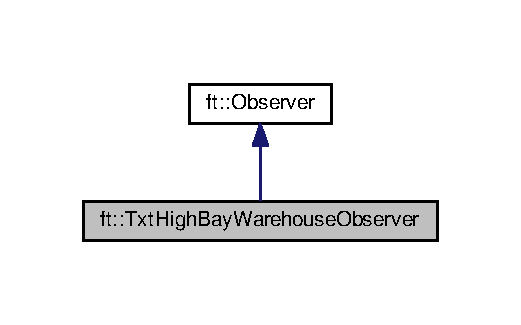
\includegraphics[width=250pt]{classft_1_1_txt_high_bay_warehouse_observer__inherit__graph}
\end{center}
\end{figure}


Collaboration diagram for ft\+:\+:Txt\+High\+Bay\+Warehouse\+Observer\+:
\nopagebreak
\begin{figure}[H]
\begin{center}
\leavevmode
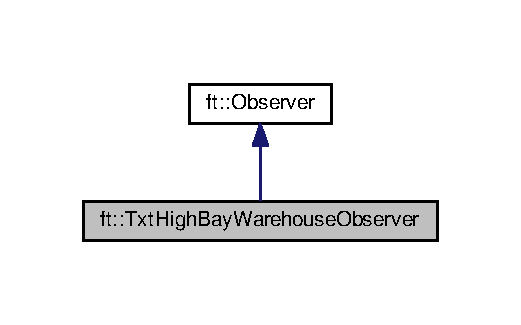
\includegraphics[width=250pt]{classft_1_1_txt_high_bay_warehouse_observer__coll__graph}
\end{center}
\end{figure}
\subsection*{Public Member Functions}
\begin{DoxyCompactItemize}
\item 
\hyperlink{classft_1_1_txt_high_bay_warehouse_observer_a12656f74e51f6a3c753ed72a05223500}{Txt\+High\+Bay\+Warehouse\+Observer} (\hyperlink{classft_1_1_txt_high_bay_warehouse}{ft\+::\+Txt\+High\+Bay\+Warehouse} $\ast$s, \hyperlink{classft_1_1_txt_mqtt_factory_client}{ft\+::\+Txt\+Mqtt\+Factory\+Client} $\ast$mqttclient)
\item 
virtual \hyperlink{classft_1_1_txt_high_bay_warehouse_observer_a15df3136540d2b4bc1a501d60a9ee61b}{$\sim$\+Txt\+High\+Bay\+Warehouse\+Observer} ()
\item 
void \hyperlink{classft_1_1_txt_high_bay_warehouse_observer_ac3519a699f526f34d39bf6be04f00ff6}{Update} (\hyperlink{classft_1_1_subject_observer}{ft\+::\+Subject\+Observer} $\ast$the\+Changed\+Subject)
\end{DoxyCompactItemize}


\subsection{Constructor \& Destructor Documentation}
\index{ft\+::\+Txt\+High\+Bay\+Warehouse\+Observer@{ft\+::\+Txt\+High\+Bay\+Warehouse\+Observer}!Txt\+High\+Bay\+Warehouse\+Observer@{Txt\+High\+Bay\+Warehouse\+Observer}}
\index{Txt\+High\+Bay\+Warehouse\+Observer@{Txt\+High\+Bay\+Warehouse\+Observer}!ft\+::\+Txt\+High\+Bay\+Warehouse\+Observer@{ft\+::\+Txt\+High\+Bay\+Warehouse\+Observer}}
\subsubsection[{\texorpdfstring{Txt\+High\+Bay\+Warehouse\+Observer(ft\+::\+Txt\+High\+Bay\+Warehouse $\ast$s, ft\+::\+Txt\+Mqtt\+Factory\+Client $\ast$mqttclient)}{TxtHighBayWarehouseObserver(ft::TxtHighBayWarehouse *s, ft::TxtMqttFactoryClient *mqttclient)}}]{\setlength{\rightskip}{0pt plus 5cm}ft\+::\+Txt\+High\+Bay\+Warehouse\+Observer\+::\+Txt\+High\+Bay\+Warehouse\+Observer (
\begin{DoxyParamCaption}
\item[{{\bf ft\+::\+Txt\+High\+Bay\+Warehouse} $\ast$}]{s, }
\item[{{\bf ft\+::\+Txt\+Mqtt\+Factory\+Client} $\ast$}]{mqttclient}
\end{DoxyParamCaption}
)\hspace{0.3cm}{\ttfamily [inline]}}\hypertarget{classft_1_1_txt_high_bay_warehouse_observer_a12656f74e51f6a3c753ed72a05223500}{}\label{classft_1_1_txt_high_bay_warehouse_observer_a12656f74e51f6a3c753ed72a05223500}
\index{ft\+::\+Txt\+High\+Bay\+Warehouse\+Observer@{ft\+::\+Txt\+High\+Bay\+Warehouse\+Observer}!````~Txt\+High\+Bay\+Warehouse\+Observer@{$\sim$\+Txt\+High\+Bay\+Warehouse\+Observer}}
\index{````~Txt\+High\+Bay\+Warehouse\+Observer@{$\sim$\+Txt\+High\+Bay\+Warehouse\+Observer}!ft\+::\+Txt\+High\+Bay\+Warehouse\+Observer@{ft\+::\+Txt\+High\+Bay\+Warehouse\+Observer}}
\subsubsection[{\texorpdfstring{$\sim$\+Txt\+High\+Bay\+Warehouse\+Observer()}{~TxtHighBayWarehouseObserver()}}]{\setlength{\rightskip}{0pt plus 5cm}virtual ft\+::\+Txt\+High\+Bay\+Warehouse\+Observer\+::$\sim$\+Txt\+High\+Bay\+Warehouse\+Observer (
\begin{DoxyParamCaption}
{}
\end{DoxyParamCaption}
)\hspace{0.3cm}{\ttfamily [inline]}, {\ttfamily [virtual]}}\hypertarget{classft_1_1_txt_high_bay_warehouse_observer_a15df3136540d2b4bc1a501d60a9ee61b}{}\label{classft_1_1_txt_high_bay_warehouse_observer_a15df3136540d2b4bc1a501d60a9ee61b}


\subsection{Member Function Documentation}
\index{ft\+::\+Txt\+High\+Bay\+Warehouse\+Observer@{ft\+::\+Txt\+High\+Bay\+Warehouse\+Observer}!Update@{Update}}
\index{Update@{Update}!ft\+::\+Txt\+High\+Bay\+Warehouse\+Observer@{ft\+::\+Txt\+High\+Bay\+Warehouse\+Observer}}
\subsubsection[{\texorpdfstring{Update(ft\+::\+Subject\+Observer $\ast$the\+Changed\+Subject)}{Update(ft::SubjectObserver *theChangedSubject)}}]{\setlength{\rightskip}{0pt plus 5cm}void ft\+::\+Txt\+High\+Bay\+Warehouse\+Observer\+::\+Update (
\begin{DoxyParamCaption}
\item[{{\bf ft\+::\+Subject\+Observer} $\ast$}]{the\+Changed\+Subject}
\end{DoxyParamCaption}
)\hspace{0.3cm}{\ttfamily [inline]}, {\ttfamily [virtual]}}\hypertarget{classft_1_1_txt_high_bay_warehouse_observer_ac3519a699f526f34d39bf6be04f00ff6}{}\label{classft_1_1_txt_high_bay_warehouse_observer_ac3519a699f526f34d39bf6be04f00ff6}


Implements \hyperlink{classft_1_1_observer_aeea41c77afbd09f595a4290954a5aa66}{ft\+::\+Observer}.



The documentation for this class was generated from the following file\+:\begin{DoxyCompactItemize}
\item 
\hyperlink{_txt_high_bay_warehouse_8h}{Txt\+High\+Bay\+Warehouse.\+h}\end{DoxyCompactItemize}

\hypertarget{classft_1_1_txt_high_bay_warehouse_storage}{}\section{ft\+:\+:Txt\+High\+Bay\+Warehouse\+Storage Class Reference}
\label{classft_1_1_txt_high_bay_warehouse_storage}\index{ft\+::\+Txt\+High\+Bay\+Warehouse\+Storage@{ft\+::\+Txt\+High\+Bay\+Warehouse\+Storage}}


{\ttfamily \#include $<$Txt\+High\+Bay\+Warehouse\+Storage.\+h$>$}



Inheritance diagram for ft\+:\+:Txt\+High\+Bay\+Warehouse\+Storage\+:
\nopagebreak
\begin{figure}[H]
\begin{center}
\leavevmode
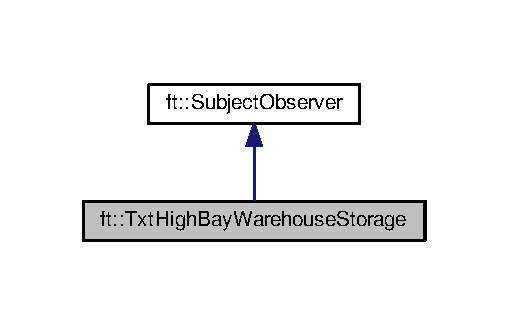
\includegraphics[width=244pt]{classft_1_1_txt_high_bay_warehouse_storage__inherit__graph}
\end{center}
\end{figure}


Collaboration diagram for ft\+:\+:Txt\+High\+Bay\+Warehouse\+Storage\+:
\nopagebreak
\begin{figure}[H]
\begin{center}
\leavevmode
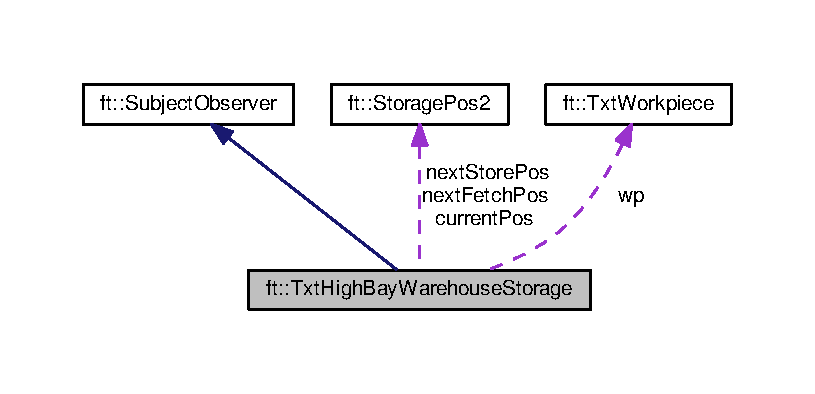
\includegraphics[width=350pt]{classft_1_1_txt_high_bay_warehouse_storage__coll__graph}
\end{center}
\end{figure}
\subsection*{Public Member Functions}
\begin{DoxyCompactItemize}
\item 
\hyperlink{classft_1_1_txt_high_bay_warehouse_storage_a4551a76f2dea3b02c788538cf5e666ec}{Txt\+High\+Bay\+Warehouse\+Storage} ()
\item 
virtual \hyperlink{classft_1_1_txt_high_bay_warehouse_storage_a69187469721bade83966bad55f05866b}{$\sim$\+Txt\+High\+Bay\+Warehouse\+Storage} ()
\item 
bool \hyperlink{classft_1_1_txt_high_bay_warehouse_storage_a1a060437a59198b8255e14d358e2ba2b}{load\+Storage\+State} ()
\item 
bool \hyperlink{classft_1_1_txt_high_bay_warehouse_storage_adf467b1079ac9da68c9060ba93549a91}{save\+Storage\+State} ()
\item 
void \hyperlink{classft_1_1_txt_high_bay_warehouse_storage_a18e8907efde4005f34a66cb61c2c6421}{reset\+Storage\+State} ()
\item 
bool \hyperlink{classft_1_1_txt_high_bay_warehouse_storage_aa55aba97bcdd43fb1e24b1d86b396f21}{store} (\hyperlink{classft_1_1_txt_workpiece}{Txt\+Workpiece} \+\_\+wp)
\item 
bool \hyperlink{classft_1_1_txt_high_bay_warehouse_storage_ac2bd0a0d9fe261f4d94788ae040b1f69}{store\+Container} ()
\item 
bool \hyperlink{classft_1_1_txt_high_bay_warehouse_storage_a242e726561dc62e093447dfd3b40067f}{fetch} (\hyperlink{namespaceft_a2d5bf01b2da29de3c061682f3195b5b2}{Txt\+W\+P\+Type\+\_\+t} t)
\item 
bool \hyperlink{classft_1_1_txt_high_bay_warehouse_storage_ab02d3081f7f2fafa7bc5a82ced5bfcaf}{fetch\+Container} ()
\item 
\hyperlink{structft_1_1_storage_pos2}{Storage\+Pos2} \hyperlink{classft_1_1_txt_high_bay_warehouse_storage_a10ac1a11e62b9bccabebb2bd5fb81d9e}{get\+Next\+Store\+Pos} ()
\item 
\hyperlink{structft_1_1_storage_pos2}{Storage\+Pos2} \hyperlink{classft_1_1_txt_high_bay_warehouse_storage_a46ba59d51380e1444c65a282d5cb9c73}{get\+Next\+Fetch\+Pos} ()
\item 
\hyperlink{structft_1_1_storage_pos2}{Storage\+Pos2} \hyperlink{classft_1_1_txt_high_bay_warehouse_storage_a33285b237647cd0922644e18b8f8f924}{get\+Current\+Pos} ()
\item 
bool \hyperlink{classft_1_1_txt_high_bay_warehouse_storage_a54b88449e3c92d468addcd83adaf8fb6}{is\+Valid\+Pos} (\hyperlink{structft_1_1_storage_pos2}{Storage\+Pos2} p)
\item 
bool \hyperlink{classft_1_1_txt_high_bay_warehouse_storage_addb4104568362975ae7a86aae00e40b1}{can\+Color\+Be\+Stored} (\hyperlink{namespaceft_a2d5bf01b2da29de3c061682f3195b5b2}{Txt\+W\+P\+Type\+\_\+t} c)
\item 
\hyperlink{namespaceft_a3d5e802a7d78dac37b288630c9b21e64}{Stock\+\_\+map\+\_\+t} \hyperlink{classft_1_1_txt_high_bay_warehouse_storage_ae9285b77591912e78024af7880bb15bc}{get\+Stock\+Map} ()
\end{DoxyCompactItemize}
\subsection*{Protected Member Functions}
\begin{DoxyCompactItemize}
\item 
char \hyperlink{classft_1_1_txt_high_bay_warehouse_storage_a878b882237dcc676f449e61a046cc198}{char\+Type} (int x, int y)
\item 
void \hyperlink{classft_1_1_txt_high_bay_warehouse_storage_a725e3c1db6fd7c4c62fcce29bb0f8af1}{print} ()
\end{DoxyCompactItemize}
\subsection*{Protected Attributes}
\begin{DoxyCompactItemize}
\item 
std\+::string \hyperlink{classft_1_1_txt_high_bay_warehouse_storage_abef4ef4c07a402eb3684969f445d509a}{filename}
\item 
\hyperlink{classft_1_1_txt_workpiece}{Txt\+Workpiece} $\ast$ \hyperlink{classft_1_1_txt_high_bay_warehouse_storage_a0e026759b179c44a78e642b338ab8694}{wp} \mbox{[}3\mbox{]}\mbox{[}3\mbox{]}
\item 
bool \hyperlink{classft_1_1_txt_high_bay_warehouse_storage_a0a570d0460997c823a04d990f08fae6f}{wpc} \mbox{[}3\mbox{]}\mbox{[}3\mbox{]}
\item 
\hyperlink{structft_1_1_storage_pos2}{Storage\+Pos2} \hyperlink{classft_1_1_txt_high_bay_warehouse_storage_a15060d4d72967a38ecd0a4348c671c3d}{current\+Pos}
\item 
\hyperlink{structft_1_1_storage_pos2}{Storage\+Pos2} \hyperlink{classft_1_1_txt_high_bay_warehouse_storage_a286ac2c5d0e3aaa944bf770725c1ac7c}{next\+Store\+Pos}
\item 
\hyperlink{structft_1_1_storage_pos2}{Storage\+Pos2} \hyperlink{classft_1_1_txt_high_bay_warehouse_storage_a46a776c37667a3f107fd1e78354e71d9}{next\+Fetch\+Pos}
\end{DoxyCompactItemize}


\subsection{Constructor \& Destructor Documentation}
\index{ft\+::\+Txt\+High\+Bay\+Warehouse\+Storage@{ft\+::\+Txt\+High\+Bay\+Warehouse\+Storage}!Txt\+High\+Bay\+Warehouse\+Storage@{Txt\+High\+Bay\+Warehouse\+Storage}}
\index{Txt\+High\+Bay\+Warehouse\+Storage@{Txt\+High\+Bay\+Warehouse\+Storage}!ft\+::\+Txt\+High\+Bay\+Warehouse\+Storage@{ft\+::\+Txt\+High\+Bay\+Warehouse\+Storage}}
\subsubsection[{\texorpdfstring{Txt\+High\+Bay\+Warehouse\+Storage()}{TxtHighBayWarehouseStorage()}}]{\setlength{\rightskip}{0pt plus 5cm}ft\+::\+Txt\+High\+Bay\+Warehouse\+Storage\+::\+Txt\+High\+Bay\+Warehouse\+Storage (
\begin{DoxyParamCaption}
{}
\end{DoxyParamCaption}
)}\hypertarget{classft_1_1_txt_high_bay_warehouse_storage_a4551a76f2dea3b02c788538cf5e666ec}{}\label{classft_1_1_txt_high_bay_warehouse_storage_a4551a76f2dea3b02c788538cf5e666ec}
\index{ft\+::\+Txt\+High\+Bay\+Warehouse\+Storage@{ft\+::\+Txt\+High\+Bay\+Warehouse\+Storage}!````~Txt\+High\+Bay\+Warehouse\+Storage@{$\sim$\+Txt\+High\+Bay\+Warehouse\+Storage}}
\index{````~Txt\+High\+Bay\+Warehouse\+Storage@{$\sim$\+Txt\+High\+Bay\+Warehouse\+Storage}!ft\+::\+Txt\+High\+Bay\+Warehouse\+Storage@{ft\+::\+Txt\+High\+Bay\+Warehouse\+Storage}}
\subsubsection[{\texorpdfstring{$\sim$\+Txt\+High\+Bay\+Warehouse\+Storage()}{~TxtHighBayWarehouseStorage()}}]{\setlength{\rightskip}{0pt plus 5cm}virtual ft\+::\+Txt\+High\+Bay\+Warehouse\+Storage\+::$\sim$\+Txt\+High\+Bay\+Warehouse\+Storage (
\begin{DoxyParamCaption}
{}
\end{DoxyParamCaption}
)\hspace{0.3cm}{\ttfamily [virtual]}}\hypertarget{classft_1_1_txt_high_bay_warehouse_storage_a69187469721bade83966bad55f05866b}{}\label{classft_1_1_txt_high_bay_warehouse_storage_a69187469721bade83966bad55f05866b}


\subsection{Member Function Documentation}
\index{ft\+::\+Txt\+High\+Bay\+Warehouse\+Storage@{ft\+::\+Txt\+High\+Bay\+Warehouse\+Storage}!can\+Color\+Be\+Stored@{can\+Color\+Be\+Stored}}
\index{can\+Color\+Be\+Stored@{can\+Color\+Be\+Stored}!ft\+::\+Txt\+High\+Bay\+Warehouse\+Storage@{ft\+::\+Txt\+High\+Bay\+Warehouse\+Storage}}
\subsubsection[{\texorpdfstring{can\+Color\+Be\+Stored(\+Txt\+W\+P\+Type\+\_\+t c)}{canColorBeStored(TxtWPType_t c)}}]{\setlength{\rightskip}{0pt plus 5cm}bool ft\+::\+Txt\+High\+Bay\+Warehouse\+Storage\+::can\+Color\+Be\+Stored (
\begin{DoxyParamCaption}
\item[{{\bf Txt\+W\+P\+Type\+\_\+t}}]{c}
\end{DoxyParamCaption}
)}\hypertarget{classft_1_1_txt_high_bay_warehouse_storage_addb4104568362975ae7a86aae00e40b1}{}\label{classft_1_1_txt_high_bay_warehouse_storage_addb4104568362975ae7a86aae00e40b1}
\index{ft\+::\+Txt\+High\+Bay\+Warehouse\+Storage@{ft\+::\+Txt\+High\+Bay\+Warehouse\+Storage}!char\+Type@{char\+Type}}
\index{char\+Type@{char\+Type}!ft\+::\+Txt\+High\+Bay\+Warehouse\+Storage@{ft\+::\+Txt\+High\+Bay\+Warehouse\+Storage}}
\subsubsection[{\texorpdfstring{char\+Type(int x, int y)}{charType(int x, int y)}}]{\setlength{\rightskip}{0pt plus 5cm}char ft\+::\+Txt\+High\+Bay\+Warehouse\+Storage\+::char\+Type (
\begin{DoxyParamCaption}
\item[{int}]{x, }
\item[{int}]{y}
\end{DoxyParamCaption}
)\hspace{0.3cm}{\ttfamily [protected]}}\hypertarget{classft_1_1_txt_high_bay_warehouse_storage_a878b882237dcc676f449e61a046cc198}{}\label{classft_1_1_txt_high_bay_warehouse_storage_a878b882237dcc676f449e61a046cc198}
\index{ft\+::\+Txt\+High\+Bay\+Warehouse\+Storage@{ft\+::\+Txt\+High\+Bay\+Warehouse\+Storage}!fetch@{fetch}}
\index{fetch@{fetch}!ft\+::\+Txt\+High\+Bay\+Warehouse\+Storage@{ft\+::\+Txt\+High\+Bay\+Warehouse\+Storage}}
\subsubsection[{\texorpdfstring{fetch(\+Txt\+W\+P\+Type\+\_\+t t)}{fetch(TxtWPType_t t)}}]{\setlength{\rightskip}{0pt plus 5cm}bool ft\+::\+Txt\+High\+Bay\+Warehouse\+Storage\+::fetch (
\begin{DoxyParamCaption}
\item[{{\bf Txt\+W\+P\+Type\+\_\+t}}]{t}
\end{DoxyParamCaption}
)}\hypertarget{classft_1_1_txt_high_bay_warehouse_storage_a242e726561dc62e093447dfd3b40067f}{}\label{classft_1_1_txt_high_bay_warehouse_storage_a242e726561dc62e093447dfd3b40067f}
\index{ft\+::\+Txt\+High\+Bay\+Warehouse\+Storage@{ft\+::\+Txt\+High\+Bay\+Warehouse\+Storage}!fetch\+Container@{fetch\+Container}}
\index{fetch\+Container@{fetch\+Container}!ft\+::\+Txt\+High\+Bay\+Warehouse\+Storage@{ft\+::\+Txt\+High\+Bay\+Warehouse\+Storage}}
\subsubsection[{\texorpdfstring{fetch\+Container()}{fetchContainer()}}]{\setlength{\rightskip}{0pt plus 5cm}bool ft\+::\+Txt\+High\+Bay\+Warehouse\+Storage\+::fetch\+Container (
\begin{DoxyParamCaption}
{}
\end{DoxyParamCaption}
)}\hypertarget{classft_1_1_txt_high_bay_warehouse_storage_ab02d3081f7f2fafa7bc5a82ced5bfcaf}{}\label{classft_1_1_txt_high_bay_warehouse_storage_ab02d3081f7f2fafa7bc5a82ced5bfcaf}
\index{ft\+::\+Txt\+High\+Bay\+Warehouse\+Storage@{ft\+::\+Txt\+High\+Bay\+Warehouse\+Storage}!get\+Current\+Pos@{get\+Current\+Pos}}
\index{get\+Current\+Pos@{get\+Current\+Pos}!ft\+::\+Txt\+High\+Bay\+Warehouse\+Storage@{ft\+::\+Txt\+High\+Bay\+Warehouse\+Storage}}
\subsubsection[{\texorpdfstring{get\+Current\+Pos()}{getCurrentPos()}}]{\setlength{\rightskip}{0pt plus 5cm}{\bf Storage\+Pos2} ft\+::\+Txt\+High\+Bay\+Warehouse\+Storage\+::get\+Current\+Pos (
\begin{DoxyParamCaption}
{}
\end{DoxyParamCaption}
)\hspace{0.3cm}{\ttfamily [inline]}}\hypertarget{classft_1_1_txt_high_bay_warehouse_storage_a33285b237647cd0922644e18b8f8f924}{}\label{classft_1_1_txt_high_bay_warehouse_storage_a33285b237647cd0922644e18b8f8f924}
\index{ft\+::\+Txt\+High\+Bay\+Warehouse\+Storage@{ft\+::\+Txt\+High\+Bay\+Warehouse\+Storage}!get\+Next\+Fetch\+Pos@{get\+Next\+Fetch\+Pos}}
\index{get\+Next\+Fetch\+Pos@{get\+Next\+Fetch\+Pos}!ft\+::\+Txt\+High\+Bay\+Warehouse\+Storage@{ft\+::\+Txt\+High\+Bay\+Warehouse\+Storage}}
\subsubsection[{\texorpdfstring{get\+Next\+Fetch\+Pos()}{getNextFetchPos()}}]{\setlength{\rightskip}{0pt plus 5cm}{\bf Storage\+Pos2} ft\+::\+Txt\+High\+Bay\+Warehouse\+Storage\+::get\+Next\+Fetch\+Pos (
\begin{DoxyParamCaption}
{}
\end{DoxyParamCaption}
)\hspace{0.3cm}{\ttfamily [inline]}}\hypertarget{classft_1_1_txt_high_bay_warehouse_storage_a46ba59d51380e1444c65a282d5cb9c73}{}\label{classft_1_1_txt_high_bay_warehouse_storage_a46ba59d51380e1444c65a282d5cb9c73}
\index{ft\+::\+Txt\+High\+Bay\+Warehouse\+Storage@{ft\+::\+Txt\+High\+Bay\+Warehouse\+Storage}!get\+Next\+Store\+Pos@{get\+Next\+Store\+Pos}}
\index{get\+Next\+Store\+Pos@{get\+Next\+Store\+Pos}!ft\+::\+Txt\+High\+Bay\+Warehouse\+Storage@{ft\+::\+Txt\+High\+Bay\+Warehouse\+Storage}}
\subsubsection[{\texorpdfstring{get\+Next\+Store\+Pos()}{getNextStorePos()}}]{\setlength{\rightskip}{0pt plus 5cm}{\bf Storage\+Pos2} ft\+::\+Txt\+High\+Bay\+Warehouse\+Storage\+::get\+Next\+Store\+Pos (
\begin{DoxyParamCaption}
{}
\end{DoxyParamCaption}
)\hspace{0.3cm}{\ttfamily [inline]}}\hypertarget{classft_1_1_txt_high_bay_warehouse_storage_a10ac1a11e62b9bccabebb2bd5fb81d9e}{}\label{classft_1_1_txt_high_bay_warehouse_storage_a10ac1a11e62b9bccabebb2bd5fb81d9e}
\index{ft\+::\+Txt\+High\+Bay\+Warehouse\+Storage@{ft\+::\+Txt\+High\+Bay\+Warehouse\+Storage}!get\+Stock\+Map@{get\+Stock\+Map}}
\index{get\+Stock\+Map@{get\+Stock\+Map}!ft\+::\+Txt\+High\+Bay\+Warehouse\+Storage@{ft\+::\+Txt\+High\+Bay\+Warehouse\+Storage}}
\subsubsection[{\texorpdfstring{get\+Stock\+Map()}{getStockMap()}}]{\setlength{\rightskip}{0pt plus 5cm}{\bf Stock\+\_\+map\+\_\+t} ft\+::\+Txt\+High\+Bay\+Warehouse\+Storage\+::get\+Stock\+Map (
\begin{DoxyParamCaption}
{}
\end{DoxyParamCaption}
)}\hypertarget{classft_1_1_txt_high_bay_warehouse_storage_ae9285b77591912e78024af7880bb15bc}{}\label{classft_1_1_txt_high_bay_warehouse_storage_ae9285b77591912e78024af7880bb15bc}
\index{ft\+::\+Txt\+High\+Bay\+Warehouse\+Storage@{ft\+::\+Txt\+High\+Bay\+Warehouse\+Storage}!is\+Valid\+Pos@{is\+Valid\+Pos}}
\index{is\+Valid\+Pos@{is\+Valid\+Pos}!ft\+::\+Txt\+High\+Bay\+Warehouse\+Storage@{ft\+::\+Txt\+High\+Bay\+Warehouse\+Storage}}
\subsubsection[{\texorpdfstring{is\+Valid\+Pos(\+Storage\+Pos2 p)}{isValidPos(StoragePos2 p)}}]{\setlength{\rightskip}{0pt plus 5cm}bool ft\+::\+Txt\+High\+Bay\+Warehouse\+Storage\+::is\+Valid\+Pos (
\begin{DoxyParamCaption}
\item[{{\bf Storage\+Pos2}}]{p}
\end{DoxyParamCaption}
)}\hypertarget{classft_1_1_txt_high_bay_warehouse_storage_a54b88449e3c92d468addcd83adaf8fb6}{}\label{classft_1_1_txt_high_bay_warehouse_storage_a54b88449e3c92d468addcd83adaf8fb6}
\index{ft\+::\+Txt\+High\+Bay\+Warehouse\+Storage@{ft\+::\+Txt\+High\+Bay\+Warehouse\+Storage}!load\+Storage\+State@{load\+Storage\+State}}
\index{load\+Storage\+State@{load\+Storage\+State}!ft\+::\+Txt\+High\+Bay\+Warehouse\+Storage@{ft\+::\+Txt\+High\+Bay\+Warehouse\+Storage}}
\subsubsection[{\texorpdfstring{load\+Storage\+State()}{loadStorageState()}}]{\setlength{\rightskip}{0pt plus 5cm}bool ft\+::\+Txt\+High\+Bay\+Warehouse\+Storage\+::load\+Storage\+State (
\begin{DoxyParamCaption}
{}
\end{DoxyParamCaption}
)}\hypertarget{classft_1_1_txt_high_bay_warehouse_storage_a1a060437a59198b8255e14d358e2ba2b}{}\label{classft_1_1_txt_high_bay_warehouse_storage_a1a060437a59198b8255e14d358e2ba2b}
\index{ft\+::\+Txt\+High\+Bay\+Warehouse\+Storage@{ft\+::\+Txt\+High\+Bay\+Warehouse\+Storage}!print@{print}}
\index{print@{print}!ft\+::\+Txt\+High\+Bay\+Warehouse\+Storage@{ft\+::\+Txt\+High\+Bay\+Warehouse\+Storage}}
\subsubsection[{\texorpdfstring{print()}{print()}}]{\setlength{\rightskip}{0pt plus 5cm}void ft\+::\+Txt\+High\+Bay\+Warehouse\+Storage\+::print (
\begin{DoxyParamCaption}
{}
\end{DoxyParamCaption}
)\hspace{0.3cm}{\ttfamily [protected]}}\hypertarget{classft_1_1_txt_high_bay_warehouse_storage_a725e3c1db6fd7c4c62fcce29bb0f8af1}{}\label{classft_1_1_txt_high_bay_warehouse_storage_a725e3c1db6fd7c4c62fcce29bb0f8af1}
\index{ft\+::\+Txt\+High\+Bay\+Warehouse\+Storage@{ft\+::\+Txt\+High\+Bay\+Warehouse\+Storage}!reset\+Storage\+State@{reset\+Storage\+State}}
\index{reset\+Storage\+State@{reset\+Storage\+State}!ft\+::\+Txt\+High\+Bay\+Warehouse\+Storage@{ft\+::\+Txt\+High\+Bay\+Warehouse\+Storage}}
\subsubsection[{\texorpdfstring{reset\+Storage\+State()}{resetStorageState()}}]{\setlength{\rightskip}{0pt plus 5cm}void ft\+::\+Txt\+High\+Bay\+Warehouse\+Storage\+::reset\+Storage\+State (
\begin{DoxyParamCaption}
{}
\end{DoxyParamCaption}
)}\hypertarget{classft_1_1_txt_high_bay_warehouse_storage_a18e8907efde4005f34a66cb61c2c6421}{}\label{classft_1_1_txt_high_bay_warehouse_storage_a18e8907efde4005f34a66cb61c2c6421}
\index{ft\+::\+Txt\+High\+Bay\+Warehouse\+Storage@{ft\+::\+Txt\+High\+Bay\+Warehouse\+Storage}!save\+Storage\+State@{save\+Storage\+State}}
\index{save\+Storage\+State@{save\+Storage\+State}!ft\+::\+Txt\+High\+Bay\+Warehouse\+Storage@{ft\+::\+Txt\+High\+Bay\+Warehouse\+Storage}}
\subsubsection[{\texorpdfstring{save\+Storage\+State()}{saveStorageState()}}]{\setlength{\rightskip}{0pt plus 5cm}bool ft\+::\+Txt\+High\+Bay\+Warehouse\+Storage\+::save\+Storage\+State (
\begin{DoxyParamCaption}
{}
\end{DoxyParamCaption}
)}\hypertarget{classft_1_1_txt_high_bay_warehouse_storage_adf467b1079ac9da68c9060ba93549a91}{}\label{classft_1_1_txt_high_bay_warehouse_storage_adf467b1079ac9da68c9060ba93549a91}
\index{ft\+::\+Txt\+High\+Bay\+Warehouse\+Storage@{ft\+::\+Txt\+High\+Bay\+Warehouse\+Storage}!store@{store}}
\index{store@{store}!ft\+::\+Txt\+High\+Bay\+Warehouse\+Storage@{ft\+::\+Txt\+High\+Bay\+Warehouse\+Storage}}
\subsubsection[{\texorpdfstring{store(\+Txt\+Workpiece \+\_\+wp)}{store(TxtWorkpiece _wp)}}]{\setlength{\rightskip}{0pt plus 5cm}bool ft\+::\+Txt\+High\+Bay\+Warehouse\+Storage\+::store (
\begin{DoxyParamCaption}
\item[{{\bf Txt\+Workpiece}}]{\+\_\+wp}
\end{DoxyParamCaption}
)}\hypertarget{classft_1_1_txt_high_bay_warehouse_storage_aa55aba97bcdd43fb1e24b1d86b396f21}{}\label{classft_1_1_txt_high_bay_warehouse_storage_aa55aba97bcdd43fb1e24b1d86b396f21}
\index{ft\+::\+Txt\+High\+Bay\+Warehouse\+Storage@{ft\+::\+Txt\+High\+Bay\+Warehouse\+Storage}!store\+Container@{store\+Container}}
\index{store\+Container@{store\+Container}!ft\+::\+Txt\+High\+Bay\+Warehouse\+Storage@{ft\+::\+Txt\+High\+Bay\+Warehouse\+Storage}}
\subsubsection[{\texorpdfstring{store\+Container()}{storeContainer()}}]{\setlength{\rightskip}{0pt plus 5cm}bool ft\+::\+Txt\+High\+Bay\+Warehouse\+Storage\+::store\+Container (
\begin{DoxyParamCaption}
{}
\end{DoxyParamCaption}
)}\hypertarget{classft_1_1_txt_high_bay_warehouse_storage_ac2bd0a0d9fe261f4d94788ae040b1f69}{}\label{classft_1_1_txt_high_bay_warehouse_storage_ac2bd0a0d9fe261f4d94788ae040b1f69}


\subsection{Member Data Documentation}
\index{ft\+::\+Txt\+High\+Bay\+Warehouse\+Storage@{ft\+::\+Txt\+High\+Bay\+Warehouse\+Storage}!current\+Pos@{current\+Pos}}
\index{current\+Pos@{current\+Pos}!ft\+::\+Txt\+High\+Bay\+Warehouse\+Storage@{ft\+::\+Txt\+High\+Bay\+Warehouse\+Storage}}
\subsubsection[{\texorpdfstring{current\+Pos}{currentPos}}]{\setlength{\rightskip}{0pt plus 5cm}{\bf Storage\+Pos2} ft\+::\+Txt\+High\+Bay\+Warehouse\+Storage\+::current\+Pos\hspace{0.3cm}{\ttfamily [protected]}}\hypertarget{classft_1_1_txt_high_bay_warehouse_storage_a15060d4d72967a38ecd0a4348c671c3d}{}\label{classft_1_1_txt_high_bay_warehouse_storage_a15060d4d72967a38ecd0a4348c671c3d}
\index{ft\+::\+Txt\+High\+Bay\+Warehouse\+Storage@{ft\+::\+Txt\+High\+Bay\+Warehouse\+Storage}!filename@{filename}}
\index{filename@{filename}!ft\+::\+Txt\+High\+Bay\+Warehouse\+Storage@{ft\+::\+Txt\+High\+Bay\+Warehouse\+Storage}}
\subsubsection[{\texorpdfstring{filename}{filename}}]{\setlength{\rightskip}{0pt plus 5cm}std\+::string ft\+::\+Txt\+High\+Bay\+Warehouse\+Storage\+::filename\hspace{0.3cm}{\ttfamily [protected]}}\hypertarget{classft_1_1_txt_high_bay_warehouse_storage_abef4ef4c07a402eb3684969f445d509a}{}\label{classft_1_1_txt_high_bay_warehouse_storage_abef4ef4c07a402eb3684969f445d509a}
\index{ft\+::\+Txt\+High\+Bay\+Warehouse\+Storage@{ft\+::\+Txt\+High\+Bay\+Warehouse\+Storage}!next\+Fetch\+Pos@{next\+Fetch\+Pos}}
\index{next\+Fetch\+Pos@{next\+Fetch\+Pos}!ft\+::\+Txt\+High\+Bay\+Warehouse\+Storage@{ft\+::\+Txt\+High\+Bay\+Warehouse\+Storage}}
\subsubsection[{\texorpdfstring{next\+Fetch\+Pos}{nextFetchPos}}]{\setlength{\rightskip}{0pt plus 5cm}{\bf Storage\+Pos2} ft\+::\+Txt\+High\+Bay\+Warehouse\+Storage\+::next\+Fetch\+Pos\hspace{0.3cm}{\ttfamily [protected]}}\hypertarget{classft_1_1_txt_high_bay_warehouse_storage_a46a776c37667a3f107fd1e78354e71d9}{}\label{classft_1_1_txt_high_bay_warehouse_storage_a46a776c37667a3f107fd1e78354e71d9}
\index{ft\+::\+Txt\+High\+Bay\+Warehouse\+Storage@{ft\+::\+Txt\+High\+Bay\+Warehouse\+Storage}!next\+Store\+Pos@{next\+Store\+Pos}}
\index{next\+Store\+Pos@{next\+Store\+Pos}!ft\+::\+Txt\+High\+Bay\+Warehouse\+Storage@{ft\+::\+Txt\+High\+Bay\+Warehouse\+Storage}}
\subsubsection[{\texorpdfstring{next\+Store\+Pos}{nextStorePos}}]{\setlength{\rightskip}{0pt plus 5cm}{\bf Storage\+Pos2} ft\+::\+Txt\+High\+Bay\+Warehouse\+Storage\+::next\+Store\+Pos\hspace{0.3cm}{\ttfamily [protected]}}\hypertarget{classft_1_1_txt_high_bay_warehouse_storage_a286ac2c5d0e3aaa944bf770725c1ac7c}{}\label{classft_1_1_txt_high_bay_warehouse_storage_a286ac2c5d0e3aaa944bf770725c1ac7c}
\index{ft\+::\+Txt\+High\+Bay\+Warehouse\+Storage@{ft\+::\+Txt\+High\+Bay\+Warehouse\+Storage}!wp@{wp}}
\index{wp@{wp}!ft\+::\+Txt\+High\+Bay\+Warehouse\+Storage@{ft\+::\+Txt\+High\+Bay\+Warehouse\+Storage}}
\subsubsection[{\texorpdfstring{wp}{wp}}]{\setlength{\rightskip}{0pt plus 5cm}{\bf Txt\+Workpiece}$\ast$ ft\+::\+Txt\+High\+Bay\+Warehouse\+Storage\+::wp\mbox{[}3\mbox{]}\mbox{[}3\mbox{]}\hspace{0.3cm}{\ttfamily [protected]}}\hypertarget{classft_1_1_txt_high_bay_warehouse_storage_a0e026759b179c44a78e642b338ab8694}{}\label{classft_1_1_txt_high_bay_warehouse_storage_a0e026759b179c44a78e642b338ab8694}
\index{ft\+::\+Txt\+High\+Bay\+Warehouse\+Storage@{ft\+::\+Txt\+High\+Bay\+Warehouse\+Storage}!wpc@{wpc}}
\index{wpc@{wpc}!ft\+::\+Txt\+High\+Bay\+Warehouse\+Storage@{ft\+::\+Txt\+High\+Bay\+Warehouse\+Storage}}
\subsubsection[{\texorpdfstring{wpc}{wpc}}]{\setlength{\rightskip}{0pt plus 5cm}bool ft\+::\+Txt\+High\+Bay\+Warehouse\+Storage\+::wpc\mbox{[}3\mbox{]}\mbox{[}3\mbox{]}\hspace{0.3cm}{\ttfamily [protected]}}\hypertarget{classft_1_1_txt_high_bay_warehouse_storage_a0a570d0460997c823a04d990f08fae6f}{}\label{classft_1_1_txt_high_bay_warehouse_storage_a0a570d0460997c823a04d990f08fae6f}


The documentation for this class was generated from the following file\+:\begin{DoxyCompactItemize}
\item 
\hyperlink{_txt_high_bay_warehouse_storage_8h}{Txt\+High\+Bay\+Warehouse\+Storage.\+h}\end{DoxyCompactItemize}

\hypertarget{classft_1_1_txt_high_bay_warehouse_storage_observer}{}\section{ft\+:\+:Txt\+High\+Bay\+Warehouse\+Storage\+Observer Class Reference}
\label{classft_1_1_txt_high_bay_warehouse_storage_observer}\index{ft\+::\+Txt\+High\+Bay\+Warehouse\+Storage\+Observer@{ft\+::\+Txt\+High\+Bay\+Warehouse\+Storage\+Observer}}


{\ttfamily \#include $<$Txt\+High\+Bay\+Warehouse\+Storage.\+h$>$}



Inheritance diagram for ft\+:\+:Txt\+High\+Bay\+Warehouse\+Storage\+Observer\+:
\nopagebreak
\begin{figure}[H]
\begin{center}
\leavevmode
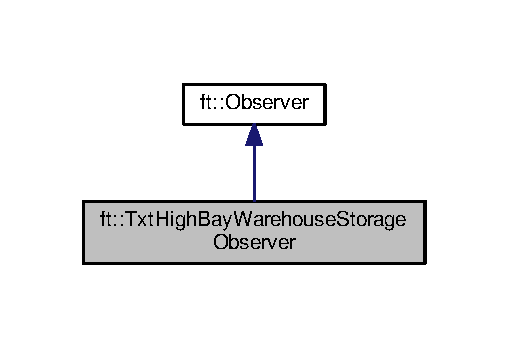
\includegraphics[width=244pt]{classft_1_1_txt_high_bay_warehouse_storage_observer__inherit__graph}
\end{center}
\end{figure}


Collaboration diagram for ft\+:\+:Txt\+High\+Bay\+Warehouse\+Storage\+Observer\+:
\nopagebreak
\begin{figure}[H]
\begin{center}
\leavevmode
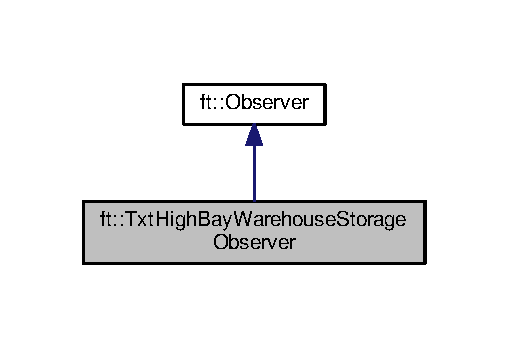
\includegraphics[width=244pt]{classft_1_1_txt_high_bay_warehouse_storage_observer__coll__graph}
\end{center}
\end{figure}
\subsection*{Public Member Functions}
\begin{DoxyCompactItemize}
\item 
\hyperlink{classft_1_1_txt_high_bay_warehouse_storage_observer_a669ec51156c8c2d5a6ffb673baf09fe6}{Txt\+High\+Bay\+Warehouse\+Storage\+Observer} (\hyperlink{classft_1_1_txt_high_bay_warehouse_storage}{ft\+::\+Txt\+High\+Bay\+Warehouse\+Storage} $\ast$s, \hyperlink{classft_1_1_txt_mqtt_factory_client}{ft\+::\+Txt\+Mqtt\+Factory\+Client} $\ast$mqttclient)
\item 
virtual \hyperlink{classft_1_1_txt_high_bay_warehouse_storage_observer_a4bae2f9bc411a0ee9cd71328cad33f35}{$\sim$\+Txt\+High\+Bay\+Warehouse\+Storage\+Observer} ()
\item 
void \hyperlink{classft_1_1_txt_high_bay_warehouse_storage_observer_a0ed13d06ea759d8840fbd1932b203b40}{Update} (\hyperlink{classft_1_1_subject_observer}{ft\+::\+Subject\+Observer} $\ast$the\+Changed\+Subject)
\end{DoxyCompactItemize}


\subsection{Constructor \& Destructor Documentation}
\index{ft\+::\+Txt\+High\+Bay\+Warehouse\+Storage\+Observer@{ft\+::\+Txt\+High\+Bay\+Warehouse\+Storage\+Observer}!Txt\+High\+Bay\+Warehouse\+Storage\+Observer@{Txt\+High\+Bay\+Warehouse\+Storage\+Observer}}
\index{Txt\+High\+Bay\+Warehouse\+Storage\+Observer@{Txt\+High\+Bay\+Warehouse\+Storage\+Observer}!ft\+::\+Txt\+High\+Bay\+Warehouse\+Storage\+Observer@{ft\+::\+Txt\+High\+Bay\+Warehouse\+Storage\+Observer}}
\subsubsection[{\texorpdfstring{Txt\+High\+Bay\+Warehouse\+Storage\+Observer(ft\+::\+Txt\+High\+Bay\+Warehouse\+Storage $\ast$s, ft\+::\+Txt\+Mqtt\+Factory\+Client $\ast$mqttclient)}{TxtHighBayWarehouseStorageObserver(ft::TxtHighBayWarehouseStorage *s, ft::TxtMqttFactoryClient *mqttclient)}}]{\setlength{\rightskip}{0pt plus 5cm}ft\+::\+Txt\+High\+Bay\+Warehouse\+Storage\+Observer\+::\+Txt\+High\+Bay\+Warehouse\+Storage\+Observer (
\begin{DoxyParamCaption}
\item[{{\bf ft\+::\+Txt\+High\+Bay\+Warehouse\+Storage} $\ast$}]{s, }
\item[{{\bf ft\+::\+Txt\+Mqtt\+Factory\+Client} $\ast$}]{mqttclient}
\end{DoxyParamCaption}
)\hspace{0.3cm}{\ttfamily [inline]}}\hypertarget{classft_1_1_txt_high_bay_warehouse_storage_observer_a669ec51156c8c2d5a6ffb673baf09fe6}{}\label{classft_1_1_txt_high_bay_warehouse_storage_observer_a669ec51156c8c2d5a6ffb673baf09fe6}
\index{ft\+::\+Txt\+High\+Bay\+Warehouse\+Storage\+Observer@{ft\+::\+Txt\+High\+Bay\+Warehouse\+Storage\+Observer}!````~Txt\+High\+Bay\+Warehouse\+Storage\+Observer@{$\sim$\+Txt\+High\+Bay\+Warehouse\+Storage\+Observer}}
\index{````~Txt\+High\+Bay\+Warehouse\+Storage\+Observer@{$\sim$\+Txt\+High\+Bay\+Warehouse\+Storage\+Observer}!ft\+::\+Txt\+High\+Bay\+Warehouse\+Storage\+Observer@{ft\+::\+Txt\+High\+Bay\+Warehouse\+Storage\+Observer}}
\subsubsection[{\texorpdfstring{$\sim$\+Txt\+High\+Bay\+Warehouse\+Storage\+Observer()}{~TxtHighBayWarehouseStorageObserver()}}]{\setlength{\rightskip}{0pt plus 5cm}virtual ft\+::\+Txt\+High\+Bay\+Warehouse\+Storage\+Observer\+::$\sim$\+Txt\+High\+Bay\+Warehouse\+Storage\+Observer (
\begin{DoxyParamCaption}
{}
\end{DoxyParamCaption}
)\hspace{0.3cm}{\ttfamily [inline]}, {\ttfamily [virtual]}}\hypertarget{classft_1_1_txt_high_bay_warehouse_storage_observer_a4bae2f9bc411a0ee9cd71328cad33f35}{}\label{classft_1_1_txt_high_bay_warehouse_storage_observer_a4bae2f9bc411a0ee9cd71328cad33f35}


\subsection{Member Function Documentation}
\index{ft\+::\+Txt\+High\+Bay\+Warehouse\+Storage\+Observer@{ft\+::\+Txt\+High\+Bay\+Warehouse\+Storage\+Observer}!Update@{Update}}
\index{Update@{Update}!ft\+::\+Txt\+High\+Bay\+Warehouse\+Storage\+Observer@{ft\+::\+Txt\+High\+Bay\+Warehouse\+Storage\+Observer}}
\subsubsection[{\texorpdfstring{Update(ft\+::\+Subject\+Observer $\ast$the\+Changed\+Subject)}{Update(ft::SubjectObserver *theChangedSubject)}}]{\setlength{\rightskip}{0pt plus 5cm}void ft\+::\+Txt\+High\+Bay\+Warehouse\+Storage\+Observer\+::\+Update (
\begin{DoxyParamCaption}
\item[{{\bf ft\+::\+Subject\+Observer} $\ast$}]{the\+Changed\+Subject}
\end{DoxyParamCaption}
)\hspace{0.3cm}{\ttfamily [inline]}, {\ttfamily [virtual]}}\hypertarget{classft_1_1_txt_high_bay_warehouse_storage_observer_a0ed13d06ea759d8840fbd1932b203b40}{}\label{classft_1_1_txt_high_bay_warehouse_storage_observer_a0ed13d06ea759d8840fbd1932b203b40}


Implements \hyperlink{classft_1_1_observer_aeea41c77afbd09f595a4290954a5aa66}{ft\+::\+Observer}.



The documentation for this class was generated from the following file\+:\begin{DoxyCompactItemize}
\item 
\hyperlink{_txt_high_bay_warehouse_storage_8h}{Txt\+High\+Bay\+Warehouse\+Storage.\+h}\end{DoxyCompactItemize}

\hypertarget{classft_1_1_txt_joysticks_data}{}\section{ft\+:\+:Txt\+Joysticks\+Data Class Reference}
\label{classft_1_1_txt_joysticks_data}\index{ft\+::\+Txt\+Joysticks\+Data@{ft\+::\+Txt\+Joysticks\+Data}}


{\ttfamily \#include $<$Txt\+Factory\+Types.\+h$>$}

\subsection*{Public Member Functions}
\begin{DoxyCompactItemize}
\item 
\hyperlink{classft_1_1_txt_joysticks_data_a13ddd352952775ada8806046722f89f8}{Txt\+Joysticks\+Data} (int \hyperlink{classft_1_1_txt_joysticks_data_afdd2de6ff6b777ec9f90bea9c3fd8b21}{a\+X1}, int \hyperlink{classft_1_1_txt_joysticks_data_a1ac5f6311efce3b5709fe1473e8ea644}{a\+Y1}, bool \hyperlink{classft_1_1_txt_joysticks_data_aeff9b78b9b8164ab6f3c2250afa3c171}{b1}, int \hyperlink{classft_1_1_txt_joysticks_data_af0719a7144158d38346658e950b3885c}{a\+X2}, int \hyperlink{classft_1_1_txt_joysticks_data_a1f0f0ab1c9ce007a12b57663343d9e9a}{a\+Y2}, bool \hyperlink{classft_1_1_txt_joysticks_data_a69e694fa165365b2498e592d7cdb17e2}{b2})
\item 
\hyperlink{classft_1_1_txt_joysticks_data_a7cae8310400b3eb35f55c450d808edf0}{Txt\+Joysticks\+Data} ()
\item 
\hyperlink{classft_1_1_txt_joysticks_data_af28ad2342115de5a200b92b7401c989c}{Txt\+Joysticks\+Data} (const \hyperlink{classft_1_1_txt_joysticks_data}{Txt\+Joysticks\+Data} \&jd)
\end{DoxyCompactItemize}
\subsection*{Public Attributes}
\begin{DoxyCompactItemize}
\item 
int \hyperlink{classft_1_1_txt_joysticks_data_afdd2de6ff6b777ec9f90bea9c3fd8b21}{a\+X1}
\item 
int \hyperlink{classft_1_1_txt_joysticks_data_a1ac5f6311efce3b5709fe1473e8ea644}{a\+Y1}
\item 
bool \hyperlink{classft_1_1_txt_joysticks_data_aeff9b78b9b8164ab6f3c2250afa3c171}{b1}
\item 
int \hyperlink{classft_1_1_txt_joysticks_data_af0719a7144158d38346658e950b3885c}{a\+X2}
\item 
int \hyperlink{classft_1_1_txt_joysticks_data_a1f0f0ab1c9ce007a12b57663343d9e9a}{a\+Y2}
\item 
bool \hyperlink{classft_1_1_txt_joysticks_data_a69e694fa165365b2498e592d7cdb17e2}{b2}
\end{DoxyCompactItemize}


\subsection{Constructor \& Destructor Documentation}
\index{ft\+::\+Txt\+Joysticks\+Data@{ft\+::\+Txt\+Joysticks\+Data}!Txt\+Joysticks\+Data@{Txt\+Joysticks\+Data}}
\index{Txt\+Joysticks\+Data@{Txt\+Joysticks\+Data}!ft\+::\+Txt\+Joysticks\+Data@{ft\+::\+Txt\+Joysticks\+Data}}
\subsubsection[{\texorpdfstring{Txt\+Joysticks\+Data(int a\+X1, int a\+Y1, bool b1, int a\+X2, int a\+Y2, bool b2)}{TxtJoysticksData(int aX1, int aY1, bool b1, int aX2, int aY2, bool b2)}}]{\setlength{\rightskip}{0pt plus 5cm}ft\+::\+Txt\+Joysticks\+Data\+::\+Txt\+Joysticks\+Data (
\begin{DoxyParamCaption}
\item[{int}]{a\+X1, }
\item[{int}]{a\+Y1, }
\item[{bool}]{b1, }
\item[{int}]{a\+X2, }
\item[{int}]{a\+Y2, }
\item[{bool}]{b2}
\end{DoxyParamCaption}
)\hspace{0.3cm}{\ttfamily [inline]}}\hypertarget{classft_1_1_txt_joysticks_data_a13ddd352952775ada8806046722f89f8}{}\label{classft_1_1_txt_joysticks_data_a13ddd352952775ada8806046722f89f8}
\index{ft\+::\+Txt\+Joysticks\+Data@{ft\+::\+Txt\+Joysticks\+Data}!Txt\+Joysticks\+Data@{Txt\+Joysticks\+Data}}
\index{Txt\+Joysticks\+Data@{Txt\+Joysticks\+Data}!ft\+::\+Txt\+Joysticks\+Data@{ft\+::\+Txt\+Joysticks\+Data}}
\subsubsection[{\texorpdfstring{Txt\+Joysticks\+Data()}{TxtJoysticksData()}}]{\setlength{\rightskip}{0pt plus 5cm}ft\+::\+Txt\+Joysticks\+Data\+::\+Txt\+Joysticks\+Data (
\begin{DoxyParamCaption}
{}
\end{DoxyParamCaption}
)\hspace{0.3cm}{\ttfamily [inline]}}\hypertarget{classft_1_1_txt_joysticks_data_a7cae8310400b3eb35f55c450d808edf0}{}\label{classft_1_1_txt_joysticks_data_a7cae8310400b3eb35f55c450d808edf0}
\index{ft\+::\+Txt\+Joysticks\+Data@{ft\+::\+Txt\+Joysticks\+Data}!Txt\+Joysticks\+Data@{Txt\+Joysticks\+Data}}
\index{Txt\+Joysticks\+Data@{Txt\+Joysticks\+Data}!ft\+::\+Txt\+Joysticks\+Data@{ft\+::\+Txt\+Joysticks\+Data}}
\subsubsection[{\texorpdfstring{Txt\+Joysticks\+Data(const Txt\+Joysticks\+Data \&jd)}{TxtJoysticksData(const TxtJoysticksData &jd)}}]{\setlength{\rightskip}{0pt plus 5cm}ft\+::\+Txt\+Joysticks\+Data\+::\+Txt\+Joysticks\+Data (
\begin{DoxyParamCaption}
\item[{const {\bf Txt\+Joysticks\+Data} \&}]{jd}
\end{DoxyParamCaption}
)\hspace{0.3cm}{\ttfamily [inline]}}\hypertarget{classft_1_1_txt_joysticks_data_af28ad2342115de5a200b92b7401c989c}{}\label{classft_1_1_txt_joysticks_data_af28ad2342115de5a200b92b7401c989c}


\subsection{Member Data Documentation}
\index{ft\+::\+Txt\+Joysticks\+Data@{ft\+::\+Txt\+Joysticks\+Data}!a\+X1@{a\+X1}}
\index{a\+X1@{a\+X1}!ft\+::\+Txt\+Joysticks\+Data@{ft\+::\+Txt\+Joysticks\+Data}}
\subsubsection[{\texorpdfstring{a\+X1}{aX1}}]{\setlength{\rightskip}{0pt plus 5cm}int ft\+::\+Txt\+Joysticks\+Data\+::a\+X1}\hypertarget{classft_1_1_txt_joysticks_data_afdd2de6ff6b777ec9f90bea9c3fd8b21}{}\label{classft_1_1_txt_joysticks_data_afdd2de6ff6b777ec9f90bea9c3fd8b21}
\index{ft\+::\+Txt\+Joysticks\+Data@{ft\+::\+Txt\+Joysticks\+Data}!a\+X2@{a\+X2}}
\index{a\+X2@{a\+X2}!ft\+::\+Txt\+Joysticks\+Data@{ft\+::\+Txt\+Joysticks\+Data}}
\subsubsection[{\texorpdfstring{a\+X2}{aX2}}]{\setlength{\rightskip}{0pt plus 5cm}int ft\+::\+Txt\+Joysticks\+Data\+::a\+X2}\hypertarget{classft_1_1_txt_joysticks_data_af0719a7144158d38346658e950b3885c}{}\label{classft_1_1_txt_joysticks_data_af0719a7144158d38346658e950b3885c}
\index{ft\+::\+Txt\+Joysticks\+Data@{ft\+::\+Txt\+Joysticks\+Data}!a\+Y1@{a\+Y1}}
\index{a\+Y1@{a\+Y1}!ft\+::\+Txt\+Joysticks\+Data@{ft\+::\+Txt\+Joysticks\+Data}}
\subsubsection[{\texorpdfstring{a\+Y1}{aY1}}]{\setlength{\rightskip}{0pt plus 5cm}int ft\+::\+Txt\+Joysticks\+Data\+::a\+Y1}\hypertarget{classft_1_1_txt_joysticks_data_a1ac5f6311efce3b5709fe1473e8ea644}{}\label{classft_1_1_txt_joysticks_data_a1ac5f6311efce3b5709fe1473e8ea644}
\index{ft\+::\+Txt\+Joysticks\+Data@{ft\+::\+Txt\+Joysticks\+Data}!a\+Y2@{a\+Y2}}
\index{a\+Y2@{a\+Y2}!ft\+::\+Txt\+Joysticks\+Data@{ft\+::\+Txt\+Joysticks\+Data}}
\subsubsection[{\texorpdfstring{a\+Y2}{aY2}}]{\setlength{\rightskip}{0pt plus 5cm}int ft\+::\+Txt\+Joysticks\+Data\+::a\+Y2}\hypertarget{classft_1_1_txt_joysticks_data_a1f0f0ab1c9ce007a12b57663343d9e9a}{}\label{classft_1_1_txt_joysticks_data_a1f0f0ab1c9ce007a12b57663343d9e9a}
\index{ft\+::\+Txt\+Joysticks\+Data@{ft\+::\+Txt\+Joysticks\+Data}!b1@{b1}}
\index{b1@{b1}!ft\+::\+Txt\+Joysticks\+Data@{ft\+::\+Txt\+Joysticks\+Data}}
\subsubsection[{\texorpdfstring{b1}{b1}}]{\setlength{\rightskip}{0pt plus 5cm}bool ft\+::\+Txt\+Joysticks\+Data\+::b1}\hypertarget{classft_1_1_txt_joysticks_data_aeff9b78b9b8164ab6f3c2250afa3c171}{}\label{classft_1_1_txt_joysticks_data_aeff9b78b9b8164ab6f3c2250afa3c171}
\index{ft\+::\+Txt\+Joysticks\+Data@{ft\+::\+Txt\+Joysticks\+Data}!b2@{b2}}
\index{b2@{b2}!ft\+::\+Txt\+Joysticks\+Data@{ft\+::\+Txt\+Joysticks\+Data}}
\subsubsection[{\texorpdfstring{b2}{b2}}]{\setlength{\rightskip}{0pt plus 5cm}bool ft\+::\+Txt\+Joysticks\+Data\+::b2}\hypertarget{classft_1_1_txt_joysticks_data_a69e694fa165365b2498e592d7cdb17e2}{}\label{classft_1_1_txt_joysticks_data_a69e694fa165365b2498e592d7cdb17e2}


The documentation for this class was generated from the following file\+:\begin{DoxyCompactItemize}
\item 
\hyperlink{_txt_factory_types_8h}{Txt\+Factory\+Types.\+h}\end{DoxyCompactItemize}

\hypertarget{classft_1_1_txt_joystick_x_y_b_controller}{}\section{ft\+:\+:Txt\+Joystick\+X\+Y\+B\+Controller Class Reference}
\label{classft_1_1_txt_joystick_x_y_b_controller}\index{ft\+::\+Txt\+Joystick\+X\+Y\+B\+Controller@{ft\+::\+Txt\+Joystick\+X\+Y\+B\+Controller}}


{\ttfamily \#include $<$Txt\+Joystick\+X\+Y\+B\+Controller.\+h$>$}



Inheritance diagram for ft\+:\+:Txt\+Joystick\+X\+Y\+B\+Controller\+:
\nopagebreak
\begin{figure}[H]
\begin{center}
\leavevmode
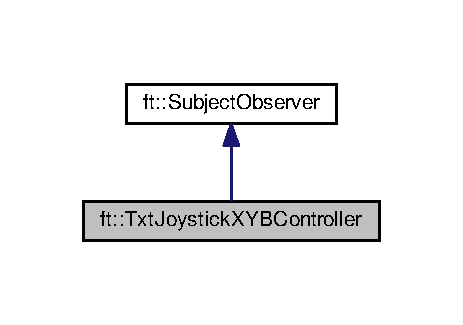
\includegraphics[width=222pt]{classft_1_1_txt_joystick_x_y_b_controller__inherit__graph}
\end{center}
\end{figure}


Collaboration diagram for ft\+:\+:Txt\+Joystick\+X\+Y\+B\+Controller\+:
\nopagebreak
\begin{figure}[H]
\begin{center}
\leavevmode
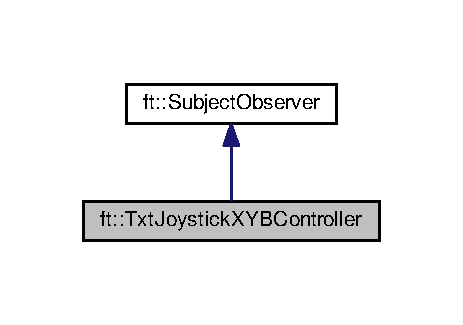
\includegraphics[width=222pt]{classft_1_1_txt_joystick_x_y_b_controller__coll__graph}
\end{center}
\end{figure}
\subsection*{Public Member Functions}
\begin{DoxyCompactItemize}
\item 
\hyperlink{classft_1_1_txt_joystick_x_y_b_controller_a90d6c8a0a5bb9ac3a91595089782810e}{Txt\+Joystick\+X\+Y\+B\+Controller} (F\+I\+S\+H\+\_\+\+X1\+\_\+\+T\+R\+A\+N\+S\+F\+ER $\ast$p\+T\+Area, uint8\+\_\+t ch\+X1, uint8\+\_\+t ch\+Y1, uint8\+\_\+t ch\+B1, uint8\+\_\+t ch\+X2, uint8\+\_\+t ch\+Y2, uint8\+\_\+t ch\+B2)
\item 
virtual \hyperlink{classft_1_1_txt_joystick_x_y_b_controller_af763355f59f61081a5095f4e2014a0a8}{$\sim$\+Txt\+Joystick\+X\+Y\+B\+Controller} ()
\item 
\hyperlink{classft_1_1_txt_joysticks_data}{Txt\+Joysticks\+Data} \hyperlink{classft_1_1_txt_joystick_x_y_b_controller_a962ddb7d0300ecddf0f2bc322bf72b26}{get\+Data} ()
\item 
bool \hyperlink{classft_1_1_txt_joystick_x_y_b_controller_aef881dfd58dcc8eead46bfcead9cdc7d}{start\+Thread} ()
\item 
bool \hyperlink{classft_1_1_txt_joystick_x_y_b_controller_afbba5442d5c9e558efc543b8c01117c1}{stop\+Thread} ()
\item 
bool \hyperlink{classft_1_1_txt_joystick_x_y_b_controller_ab56c6b61f902e08d32bdfa6d3efefc48}{is\+Thread\+Running} ()
\end{DoxyCompactItemize}
\subsection*{Public Attributes}
\begin{DoxyCompactItemize}
\item 
const int \hyperlink{classft_1_1_txt_joystick_x_y_b_controller_aed636918b23f3952bb7c7ee89d86f689}{J\+O\+Y\+\_\+\+M\+I\+N\+\_\+\+TH} = 7
\item 
const int \hyperlink{classft_1_1_txt_joystick_x_y_b_controller_a6332209742ebf5aff942f11daede67f2}{center0} = 4100
\item 
const int \hyperlink{classft_1_1_txt_joystick_x_y_b_controller_ab4a3b0a551b668871f516cf3d8ef0cc0}{delta0} = 1500
\end{DoxyCompactItemize}


\subsection{Constructor \& Destructor Documentation}
\index{ft\+::\+Txt\+Joystick\+X\+Y\+B\+Controller@{ft\+::\+Txt\+Joystick\+X\+Y\+B\+Controller}!Txt\+Joystick\+X\+Y\+B\+Controller@{Txt\+Joystick\+X\+Y\+B\+Controller}}
\index{Txt\+Joystick\+X\+Y\+B\+Controller@{Txt\+Joystick\+X\+Y\+B\+Controller}!ft\+::\+Txt\+Joystick\+X\+Y\+B\+Controller@{ft\+::\+Txt\+Joystick\+X\+Y\+B\+Controller}}
\subsubsection[{\texorpdfstring{Txt\+Joystick\+X\+Y\+B\+Controller(\+F\+I\+S\+H\+\_\+\+X1\+\_\+\+T\+R\+A\+N\+S\+F\+E\+R $\ast$p\+T\+Area, uint8\+\_\+t ch\+X1, uint8\+\_\+t ch\+Y1, uint8\+\_\+t ch\+B1, uint8\+\_\+t ch\+X2, uint8\+\_\+t ch\+Y2, uint8\+\_\+t ch\+B2)}{TxtJoystickXYBController(FISH_X1_TRANSFER *pTArea, uint8_t chX1, uint8_t chY1, uint8_t chB1, uint8_t chX2, uint8_t chY2, uint8_t chB2)}}]{\setlength{\rightskip}{0pt plus 5cm}ft\+::\+Txt\+Joystick\+X\+Y\+B\+Controller\+::\+Txt\+Joystick\+X\+Y\+B\+Controller (
\begin{DoxyParamCaption}
\item[{F\+I\+S\+H\+\_\+\+X1\+\_\+\+T\+R\+A\+N\+S\+F\+ER $\ast$}]{p\+T\+Area, }
\item[{uint8\+\_\+t}]{ch\+X1, }
\item[{uint8\+\_\+t}]{ch\+Y1, }
\item[{uint8\+\_\+t}]{ch\+B1, }
\item[{uint8\+\_\+t}]{ch\+X2, }
\item[{uint8\+\_\+t}]{ch\+Y2, }
\item[{uint8\+\_\+t}]{ch\+B2}
\end{DoxyParamCaption}
)}\hypertarget{classft_1_1_txt_joystick_x_y_b_controller_a90d6c8a0a5bb9ac3a91595089782810e}{}\label{classft_1_1_txt_joystick_x_y_b_controller_a90d6c8a0a5bb9ac3a91595089782810e}
\index{ft\+::\+Txt\+Joystick\+X\+Y\+B\+Controller@{ft\+::\+Txt\+Joystick\+X\+Y\+B\+Controller}!````~Txt\+Joystick\+X\+Y\+B\+Controller@{$\sim$\+Txt\+Joystick\+X\+Y\+B\+Controller}}
\index{````~Txt\+Joystick\+X\+Y\+B\+Controller@{$\sim$\+Txt\+Joystick\+X\+Y\+B\+Controller}!ft\+::\+Txt\+Joystick\+X\+Y\+B\+Controller@{ft\+::\+Txt\+Joystick\+X\+Y\+B\+Controller}}
\subsubsection[{\texorpdfstring{$\sim$\+Txt\+Joystick\+X\+Y\+B\+Controller()}{~TxtJoystickXYBController()}}]{\setlength{\rightskip}{0pt plus 5cm}virtual ft\+::\+Txt\+Joystick\+X\+Y\+B\+Controller\+::$\sim$\+Txt\+Joystick\+X\+Y\+B\+Controller (
\begin{DoxyParamCaption}
{}
\end{DoxyParamCaption}
)\hspace{0.3cm}{\ttfamily [virtual]}}\hypertarget{classft_1_1_txt_joystick_x_y_b_controller_af763355f59f61081a5095f4e2014a0a8}{}\label{classft_1_1_txt_joystick_x_y_b_controller_af763355f59f61081a5095f4e2014a0a8}


\subsection{Member Function Documentation}
\index{ft\+::\+Txt\+Joystick\+X\+Y\+B\+Controller@{ft\+::\+Txt\+Joystick\+X\+Y\+B\+Controller}!get\+Data@{get\+Data}}
\index{get\+Data@{get\+Data}!ft\+::\+Txt\+Joystick\+X\+Y\+B\+Controller@{ft\+::\+Txt\+Joystick\+X\+Y\+B\+Controller}}
\subsubsection[{\texorpdfstring{get\+Data()}{getData()}}]{\setlength{\rightskip}{0pt plus 5cm}{\bf Txt\+Joysticks\+Data} ft\+::\+Txt\+Joystick\+X\+Y\+B\+Controller\+::get\+Data (
\begin{DoxyParamCaption}
{}
\end{DoxyParamCaption}
)\hspace{0.3cm}{\ttfamily [inline]}}\hypertarget{classft_1_1_txt_joystick_x_y_b_controller_a962ddb7d0300ecddf0f2bc322bf72b26}{}\label{classft_1_1_txt_joystick_x_y_b_controller_a962ddb7d0300ecddf0f2bc322bf72b26}
\index{ft\+::\+Txt\+Joystick\+X\+Y\+B\+Controller@{ft\+::\+Txt\+Joystick\+X\+Y\+B\+Controller}!is\+Thread\+Running@{is\+Thread\+Running}}
\index{is\+Thread\+Running@{is\+Thread\+Running}!ft\+::\+Txt\+Joystick\+X\+Y\+B\+Controller@{ft\+::\+Txt\+Joystick\+X\+Y\+B\+Controller}}
\subsubsection[{\texorpdfstring{is\+Thread\+Running()}{isThreadRunning()}}]{\setlength{\rightskip}{0pt plus 5cm}bool ft\+::\+Txt\+Joystick\+X\+Y\+B\+Controller\+::is\+Thread\+Running (
\begin{DoxyParamCaption}
{}
\end{DoxyParamCaption}
)\hspace{0.3cm}{\ttfamily [inline]}}\hypertarget{classft_1_1_txt_joystick_x_y_b_controller_ab56c6b61f902e08d32bdfa6d3efefc48}{}\label{classft_1_1_txt_joystick_x_y_b_controller_ab56c6b61f902e08d32bdfa6d3efefc48}
\index{ft\+::\+Txt\+Joystick\+X\+Y\+B\+Controller@{ft\+::\+Txt\+Joystick\+X\+Y\+B\+Controller}!start\+Thread@{start\+Thread}}
\index{start\+Thread@{start\+Thread}!ft\+::\+Txt\+Joystick\+X\+Y\+B\+Controller@{ft\+::\+Txt\+Joystick\+X\+Y\+B\+Controller}}
\subsubsection[{\texorpdfstring{start\+Thread()}{startThread()}}]{\setlength{\rightskip}{0pt plus 5cm}bool ft\+::\+Txt\+Joystick\+X\+Y\+B\+Controller\+::start\+Thread (
\begin{DoxyParamCaption}
{}
\end{DoxyParamCaption}
)}\hypertarget{classft_1_1_txt_joystick_x_y_b_controller_aef881dfd58dcc8eead46bfcead9cdc7d}{}\label{classft_1_1_txt_joystick_x_y_b_controller_aef881dfd58dcc8eead46bfcead9cdc7d}
\index{ft\+::\+Txt\+Joystick\+X\+Y\+B\+Controller@{ft\+::\+Txt\+Joystick\+X\+Y\+B\+Controller}!stop\+Thread@{stop\+Thread}}
\index{stop\+Thread@{stop\+Thread}!ft\+::\+Txt\+Joystick\+X\+Y\+B\+Controller@{ft\+::\+Txt\+Joystick\+X\+Y\+B\+Controller}}
\subsubsection[{\texorpdfstring{stop\+Thread()}{stopThread()}}]{\setlength{\rightskip}{0pt plus 5cm}bool ft\+::\+Txt\+Joystick\+X\+Y\+B\+Controller\+::stop\+Thread (
\begin{DoxyParamCaption}
{}
\end{DoxyParamCaption}
)}\hypertarget{classft_1_1_txt_joystick_x_y_b_controller_afbba5442d5c9e558efc543b8c01117c1}{}\label{classft_1_1_txt_joystick_x_y_b_controller_afbba5442d5c9e558efc543b8c01117c1}


\subsection{Member Data Documentation}
\index{ft\+::\+Txt\+Joystick\+X\+Y\+B\+Controller@{ft\+::\+Txt\+Joystick\+X\+Y\+B\+Controller}!center0@{center0}}
\index{center0@{center0}!ft\+::\+Txt\+Joystick\+X\+Y\+B\+Controller@{ft\+::\+Txt\+Joystick\+X\+Y\+B\+Controller}}
\subsubsection[{\texorpdfstring{center0}{center0}}]{\setlength{\rightskip}{0pt plus 5cm}const int ft\+::\+Txt\+Joystick\+X\+Y\+B\+Controller\+::center0 = 4100}\hypertarget{classft_1_1_txt_joystick_x_y_b_controller_a6332209742ebf5aff942f11daede67f2}{}\label{classft_1_1_txt_joystick_x_y_b_controller_a6332209742ebf5aff942f11daede67f2}
\index{ft\+::\+Txt\+Joystick\+X\+Y\+B\+Controller@{ft\+::\+Txt\+Joystick\+X\+Y\+B\+Controller}!delta0@{delta0}}
\index{delta0@{delta0}!ft\+::\+Txt\+Joystick\+X\+Y\+B\+Controller@{ft\+::\+Txt\+Joystick\+X\+Y\+B\+Controller}}
\subsubsection[{\texorpdfstring{delta0}{delta0}}]{\setlength{\rightskip}{0pt plus 5cm}const int ft\+::\+Txt\+Joystick\+X\+Y\+B\+Controller\+::delta0 = 1500}\hypertarget{classft_1_1_txt_joystick_x_y_b_controller_ab4a3b0a551b668871f516cf3d8ef0cc0}{}\label{classft_1_1_txt_joystick_x_y_b_controller_ab4a3b0a551b668871f516cf3d8ef0cc0}
\index{ft\+::\+Txt\+Joystick\+X\+Y\+B\+Controller@{ft\+::\+Txt\+Joystick\+X\+Y\+B\+Controller}!J\+O\+Y\+\_\+\+M\+I\+N\+\_\+\+TH@{J\+O\+Y\+\_\+\+M\+I\+N\+\_\+\+TH}}
\index{J\+O\+Y\+\_\+\+M\+I\+N\+\_\+\+TH@{J\+O\+Y\+\_\+\+M\+I\+N\+\_\+\+TH}!ft\+::\+Txt\+Joystick\+X\+Y\+B\+Controller@{ft\+::\+Txt\+Joystick\+X\+Y\+B\+Controller}}
\subsubsection[{\texorpdfstring{J\+O\+Y\+\_\+\+M\+I\+N\+\_\+\+TH}{JOY_MIN_TH}}]{\setlength{\rightskip}{0pt plus 5cm}const int ft\+::\+Txt\+Joystick\+X\+Y\+B\+Controller\+::\+J\+O\+Y\+\_\+\+M\+I\+N\+\_\+\+TH = 7}\hypertarget{classft_1_1_txt_joystick_x_y_b_controller_aed636918b23f3952bb7c7ee89d86f689}{}\label{classft_1_1_txt_joystick_x_y_b_controller_aed636918b23f3952bb7c7ee89d86f689}


The documentation for this class was generated from the following file\+:\begin{DoxyCompactItemize}
\item 
\hyperlink{_txt_joystick_x_y_b_controller_8h}{Txt\+Joystick\+X\+Y\+B\+Controller.\+h}\end{DoxyCompactItemize}

\hypertarget{classft_1_1_txt_motion_detection}{}\section{ft\+:\+:Txt\+Motion\+Detection Class Reference}
\label{classft_1_1_txt_motion_detection}\index{ft\+::\+Txt\+Motion\+Detection@{ft\+::\+Txt\+Motion\+Detection}}


{\ttfamily \#include $<$Txt\+Motion\+Detection.\+h$>$}



Inheritance diagram for ft\+:\+:Txt\+Motion\+Detection\+:
\nopagebreak
\begin{figure}[H]
\begin{center}
\leavevmode
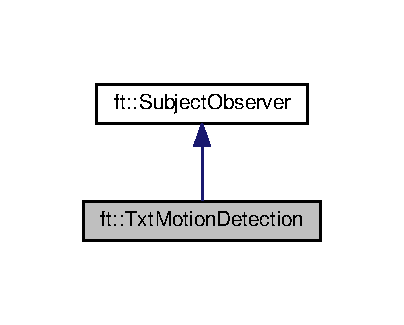
\includegraphics[width=194pt]{classft_1_1_txt_motion_detection__inherit__graph}
\end{center}
\end{figure}


Collaboration diagram for ft\+:\+:Txt\+Motion\+Detection\+:
\nopagebreak
\begin{figure}[H]
\begin{center}
\leavevmode
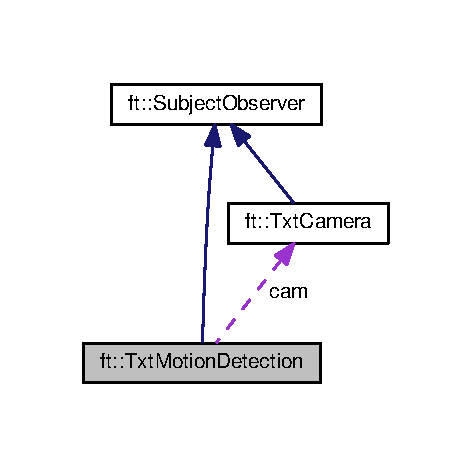
\includegraphics[width=227pt]{classft_1_1_txt_motion_detection__coll__graph}
\end{center}
\end{figure}
\subsection*{Public Member Functions}
\begin{DoxyCompactItemize}
\item 
\hyperlink{classft_1_1_txt_motion_detection_a25f406788eeb041eeec88a058185062d}{Txt\+Motion\+Detection} (\hyperlink{classft_1_1_txt_camera}{ft\+::\+Txt\+Camera} $\ast$\hyperlink{classft_1_1_txt_motion_detection_a0fcc4c62dbeb1839d705045e1a8473ad}{cam}, double \hyperlink{classft_1_1_txt_motion_detection_a6f681c16ea2ae02579eddaa0046662c6}{max\+\_\+limit\+\_\+\+Area})
\item 
virtual \hyperlink{classft_1_1_txt_motion_detection_a78177169e6e08606337ee5714ab73daa}{$\sim$\+Txt\+Motion\+Detection} ()
\item 
bool \hyperlink{classft_1_1_txt_motion_detection_ac1fa56ffd0e8ff3d6b55c128b4c2f7a7}{init} ()
\item 
bool \hyperlink{classft_1_1_txt_motion_detection_aff17b71df6cb5d0f7b213100bb4f4ac3}{start\+Thread} ()
\item 
bool \hyperlink{classft_1_1_txt_motion_detection_a1fbb361b7a5872ab28a96c7eaf4d7d13}{stop\+Thread} ()
\item 
std\+::string \hyperlink{classft_1_1_txt_motion_detection_a36924977e1c1f056508659b9f276cea1}{get\+Data\+String} ()
\end{DoxyCompactItemize}
\subsection*{Protected Member Functions}
\begin{DoxyCompactItemize}
\item 
void \hyperlink{classft_1_1_txt_motion_detection_a5cde1079735e8da9986f50bb6a32fec9}{run} ()
\end{DoxyCompactItemize}
\subsection*{Static Protected Member Functions}
\begin{DoxyCompactItemize}
\item 
static void $\ast$ \hyperlink{classft_1_1_txt_motion_detection_a032ad6f0adedc9921843585dc211b52e}{start\+\_\+thread} (void $\ast$obj)
\end{DoxyCompactItemize}
\subsection*{Protected Attributes}
\begin{DoxyCompactItemize}
\item 
\hyperlink{classft_1_1_txt_camera}{ft\+::\+Txt\+Camera} $\ast$ \hyperlink{classft_1_1_txt_motion_detection_a0fcc4c62dbeb1839d705045e1a8473ad}{cam}
\item 
cv\+::\+Mat \hyperlink{classft_1_1_txt_motion_detection_a60bf3703bf1a9d4d2c748504ac5330f3}{gray\+\_\+last}
\item 
std\+::chrono\+::system\+\_\+clock\+::time\+\_\+point \hyperlink{classft_1_1_txt_motion_detection_a5df0ee20308db61c230e17582f3e56bf}{ts\+Last\+Detected}
\item 
double \hyperlink{classft_1_1_txt_motion_detection_a6f681c16ea2ae02579eddaa0046662c6}{max\+\_\+limit\+\_\+\+Area}
\item 
volatile bool \hyperlink{classft_1_1_txt_motion_detection_a8d8e0b1cbdc411fb804be5bce190d8ec}{m\+\_\+stoprequested}
\item 
volatile bool \hyperlink{classft_1_1_txt_motion_detection_a29ef96c1c37ecb15234e5eb2b2d4fe97}{m\+\_\+running}
\item 
pthread\+\_\+mutex\+\_\+t \hyperlink{classft_1_1_txt_motion_detection_a5376f343930aa6553381fbb4faeac32f}{m\+\_\+mutex}
\item 
pthread\+\_\+t \hyperlink{classft_1_1_txt_motion_detection_a4675c4835955d3ee2cbe0f79f7ef5ead}{m\+\_\+thread}
\end{DoxyCompactItemize}


\subsection{Constructor \& Destructor Documentation}
\index{ft\+::\+Txt\+Motion\+Detection@{ft\+::\+Txt\+Motion\+Detection}!Txt\+Motion\+Detection@{Txt\+Motion\+Detection}}
\index{Txt\+Motion\+Detection@{Txt\+Motion\+Detection}!ft\+::\+Txt\+Motion\+Detection@{ft\+::\+Txt\+Motion\+Detection}}
\subsubsection[{\texorpdfstring{Txt\+Motion\+Detection(ft\+::\+Txt\+Camera $\ast$cam, double max\+\_\+limit\+\_\+\+Area)}{TxtMotionDetection(ft::TxtCamera *cam, double max_limit_Area)}}]{\setlength{\rightskip}{0pt plus 5cm}ft\+::\+Txt\+Motion\+Detection\+::\+Txt\+Motion\+Detection (
\begin{DoxyParamCaption}
\item[{{\bf ft\+::\+Txt\+Camera} $\ast$}]{cam, }
\item[{double}]{max\+\_\+limit\+\_\+\+Area}
\end{DoxyParamCaption}
)}\hypertarget{classft_1_1_txt_motion_detection_a25f406788eeb041eeec88a058185062d}{}\label{classft_1_1_txt_motion_detection_a25f406788eeb041eeec88a058185062d}
\index{ft\+::\+Txt\+Motion\+Detection@{ft\+::\+Txt\+Motion\+Detection}!````~Txt\+Motion\+Detection@{$\sim$\+Txt\+Motion\+Detection}}
\index{````~Txt\+Motion\+Detection@{$\sim$\+Txt\+Motion\+Detection}!ft\+::\+Txt\+Motion\+Detection@{ft\+::\+Txt\+Motion\+Detection}}
\subsubsection[{\texorpdfstring{$\sim$\+Txt\+Motion\+Detection()}{~TxtMotionDetection()}}]{\setlength{\rightskip}{0pt plus 5cm}virtual ft\+::\+Txt\+Motion\+Detection\+::$\sim$\+Txt\+Motion\+Detection (
\begin{DoxyParamCaption}
{}
\end{DoxyParamCaption}
)\hspace{0.3cm}{\ttfamily [virtual]}}\hypertarget{classft_1_1_txt_motion_detection_a78177169e6e08606337ee5714ab73daa}{}\label{classft_1_1_txt_motion_detection_a78177169e6e08606337ee5714ab73daa}


\subsection{Member Function Documentation}
\index{ft\+::\+Txt\+Motion\+Detection@{ft\+::\+Txt\+Motion\+Detection}!get\+Data\+String@{get\+Data\+String}}
\index{get\+Data\+String@{get\+Data\+String}!ft\+::\+Txt\+Motion\+Detection@{ft\+::\+Txt\+Motion\+Detection}}
\subsubsection[{\texorpdfstring{get\+Data\+String()}{getDataString()}}]{\setlength{\rightskip}{0pt plus 5cm}std\+::string ft\+::\+Txt\+Motion\+Detection\+::get\+Data\+String (
\begin{DoxyParamCaption}
{}
\end{DoxyParamCaption}
)}\hypertarget{classft_1_1_txt_motion_detection_a36924977e1c1f056508659b9f276cea1}{}\label{classft_1_1_txt_motion_detection_a36924977e1c1f056508659b9f276cea1}
\index{ft\+::\+Txt\+Motion\+Detection@{ft\+::\+Txt\+Motion\+Detection}!init@{init}}
\index{init@{init}!ft\+::\+Txt\+Motion\+Detection@{ft\+::\+Txt\+Motion\+Detection}}
\subsubsection[{\texorpdfstring{init()}{init()}}]{\setlength{\rightskip}{0pt plus 5cm}bool ft\+::\+Txt\+Motion\+Detection\+::init (
\begin{DoxyParamCaption}
{}
\end{DoxyParamCaption}
)}\hypertarget{classft_1_1_txt_motion_detection_ac1fa56ffd0e8ff3d6b55c128b4c2f7a7}{}\label{classft_1_1_txt_motion_detection_ac1fa56ffd0e8ff3d6b55c128b4c2f7a7}
\index{ft\+::\+Txt\+Motion\+Detection@{ft\+::\+Txt\+Motion\+Detection}!run@{run}}
\index{run@{run}!ft\+::\+Txt\+Motion\+Detection@{ft\+::\+Txt\+Motion\+Detection}}
\subsubsection[{\texorpdfstring{run()}{run()}}]{\setlength{\rightskip}{0pt plus 5cm}void ft\+::\+Txt\+Motion\+Detection\+::run (
\begin{DoxyParamCaption}
{}
\end{DoxyParamCaption}
)\hspace{0.3cm}{\ttfamily [protected]}}\hypertarget{classft_1_1_txt_motion_detection_a5cde1079735e8da9986f50bb6a32fec9}{}\label{classft_1_1_txt_motion_detection_a5cde1079735e8da9986f50bb6a32fec9}
\index{ft\+::\+Txt\+Motion\+Detection@{ft\+::\+Txt\+Motion\+Detection}!start\+\_\+thread@{start\+\_\+thread}}
\index{start\+\_\+thread@{start\+\_\+thread}!ft\+::\+Txt\+Motion\+Detection@{ft\+::\+Txt\+Motion\+Detection}}
\subsubsection[{\texorpdfstring{start\+\_\+thread(void $\ast$obj)}{start_thread(void *obj)}}]{\setlength{\rightskip}{0pt plus 5cm}static void$\ast$ ft\+::\+Txt\+Motion\+Detection\+::start\+\_\+thread (
\begin{DoxyParamCaption}
\item[{void $\ast$}]{obj}
\end{DoxyParamCaption}
)\hspace{0.3cm}{\ttfamily [inline]}, {\ttfamily [static]}, {\ttfamily [protected]}}\hypertarget{classft_1_1_txt_motion_detection_a032ad6f0adedc9921843585dc211b52e}{}\label{classft_1_1_txt_motion_detection_a032ad6f0adedc9921843585dc211b52e}
\index{ft\+::\+Txt\+Motion\+Detection@{ft\+::\+Txt\+Motion\+Detection}!start\+Thread@{start\+Thread}}
\index{start\+Thread@{start\+Thread}!ft\+::\+Txt\+Motion\+Detection@{ft\+::\+Txt\+Motion\+Detection}}
\subsubsection[{\texorpdfstring{start\+Thread()}{startThread()}}]{\setlength{\rightskip}{0pt plus 5cm}bool ft\+::\+Txt\+Motion\+Detection\+::start\+Thread (
\begin{DoxyParamCaption}
{}
\end{DoxyParamCaption}
)}\hypertarget{classft_1_1_txt_motion_detection_aff17b71df6cb5d0f7b213100bb4f4ac3}{}\label{classft_1_1_txt_motion_detection_aff17b71df6cb5d0f7b213100bb4f4ac3}
\index{ft\+::\+Txt\+Motion\+Detection@{ft\+::\+Txt\+Motion\+Detection}!stop\+Thread@{stop\+Thread}}
\index{stop\+Thread@{stop\+Thread}!ft\+::\+Txt\+Motion\+Detection@{ft\+::\+Txt\+Motion\+Detection}}
\subsubsection[{\texorpdfstring{stop\+Thread()}{stopThread()}}]{\setlength{\rightskip}{0pt plus 5cm}bool ft\+::\+Txt\+Motion\+Detection\+::stop\+Thread (
\begin{DoxyParamCaption}
{}
\end{DoxyParamCaption}
)}\hypertarget{classft_1_1_txt_motion_detection_a1fbb361b7a5872ab28a96c7eaf4d7d13}{}\label{classft_1_1_txt_motion_detection_a1fbb361b7a5872ab28a96c7eaf4d7d13}


\subsection{Member Data Documentation}
\index{ft\+::\+Txt\+Motion\+Detection@{ft\+::\+Txt\+Motion\+Detection}!cam@{cam}}
\index{cam@{cam}!ft\+::\+Txt\+Motion\+Detection@{ft\+::\+Txt\+Motion\+Detection}}
\subsubsection[{\texorpdfstring{cam}{cam}}]{\setlength{\rightskip}{0pt plus 5cm}{\bf ft\+::\+Txt\+Camera}$\ast$ ft\+::\+Txt\+Motion\+Detection\+::cam\hspace{0.3cm}{\ttfamily [protected]}}\hypertarget{classft_1_1_txt_motion_detection_a0fcc4c62dbeb1839d705045e1a8473ad}{}\label{classft_1_1_txt_motion_detection_a0fcc4c62dbeb1839d705045e1a8473ad}
\index{ft\+::\+Txt\+Motion\+Detection@{ft\+::\+Txt\+Motion\+Detection}!gray\+\_\+last@{gray\+\_\+last}}
\index{gray\+\_\+last@{gray\+\_\+last}!ft\+::\+Txt\+Motion\+Detection@{ft\+::\+Txt\+Motion\+Detection}}
\subsubsection[{\texorpdfstring{gray\+\_\+last}{gray_last}}]{\setlength{\rightskip}{0pt plus 5cm}cv\+::\+Mat ft\+::\+Txt\+Motion\+Detection\+::gray\+\_\+last\hspace{0.3cm}{\ttfamily [protected]}}\hypertarget{classft_1_1_txt_motion_detection_a60bf3703bf1a9d4d2c748504ac5330f3}{}\label{classft_1_1_txt_motion_detection_a60bf3703bf1a9d4d2c748504ac5330f3}
\index{ft\+::\+Txt\+Motion\+Detection@{ft\+::\+Txt\+Motion\+Detection}!m\+\_\+mutex@{m\+\_\+mutex}}
\index{m\+\_\+mutex@{m\+\_\+mutex}!ft\+::\+Txt\+Motion\+Detection@{ft\+::\+Txt\+Motion\+Detection}}
\subsubsection[{\texorpdfstring{m\+\_\+mutex}{m_mutex}}]{\setlength{\rightskip}{0pt plus 5cm}pthread\+\_\+mutex\+\_\+t ft\+::\+Txt\+Motion\+Detection\+::m\+\_\+mutex\hspace{0.3cm}{\ttfamily [protected]}}\hypertarget{classft_1_1_txt_motion_detection_a5376f343930aa6553381fbb4faeac32f}{}\label{classft_1_1_txt_motion_detection_a5376f343930aa6553381fbb4faeac32f}
\index{ft\+::\+Txt\+Motion\+Detection@{ft\+::\+Txt\+Motion\+Detection}!m\+\_\+running@{m\+\_\+running}}
\index{m\+\_\+running@{m\+\_\+running}!ft\+::\+Txt\+Motion\+Detection@{ft\+::\+Txt\+Motion\+Detection}}
\subsubsection[{\texorpdfstring{m\+\_\+running}{m_running}}]{\setlength{\rightskip}{0pt plus 5cm}volatile bool ft\+::\+Txt\+Motion\+Detection\+::m\+\_\+running\hspace{0.3cm}{\ttfamily [protected]}}\hypertarget{classft_1_1_txt_motion_detection_a29ef96c1c37ecb15234e5eb2b2d4fe97}{}\label{classft_1_1_txt_motion_detection_a29ef96c1c37ecb15234e5eb2b2d4fe97}
\index{ft\+::\+Txt\+Motion\+Detection@{ft\+::\+Txt\+Motion\+Detection}!m\+\_\+stoprequested@{m\+\_\+stoprequested}}
\index{m\+\_\+stoprequested@{m\+\_\+stoprequested}!ft\+::\+Txt\+Motion\+Detection@{ft\+::\+Txt\+Motion\+Detection}}
\subsubsection[{\texorpdfstring{m\+\_\+stoprequested}{m_stoprequested}}]{\setlength{\rightskip}{0pt plus 5cm}volatile bool ft\+::\+Txt\+Motion\+Detection\+::m\+\_\+stoprequested\hspace{0.3cm}{\ttfamily [protected]}}\hypertarget{classft_1_1_txt_motion_detection_a8d8e0b1cbdc411fb804be5bce190d8ec}{}\label{classft_1_1_txt_motion_detection_a8d8e0b1cbdc411fb804be5bce190d8ec}
\index{ft\+::\+Txt\+Motion\+Detection@{ft\+::\+Txt\+Motion\+Detection}!m\+\_\+thread@{m\+\_\+thread}}
\index{m\+\_\+thread@{m\+\_\+thread}!ft\+::\+Txt\+Motion\+Detection@{ft\+::\+Txt\+Motion\+Detection}}
\subsubsection[{\texorpdfstring{m\+\_\+thread}{m_thread}}]{\setlength{\rightskip}{0pt plus 5cm}pthread\+\_\+t ft\+::\+Txt\+Motion\+Detection\+::m\+\_\+thread\hspace{0.3cm}{\ttfamily [protected]}}\hypertarget{classft_1_1_txt_motion_detection_a4675c4835955d3ee2cbe0f79f7ef5ead}{}\label{classft_1_1_txt_motion_detection_a4675c4835955d3ee2cbe0f79f7ef5ead}
\index{ft\+::\+Txt\+Motion\+Detection@{ft\+::\+Txt\+Motion\+Detection}!max\+\_\+limit\+\_\+\+Area@{max\+\_\+limit\+\_\+\+Area}}
\index{max\+\_\+limit\+\_\+\+Area@{max\+\_\+limit\+\_\+\+Area}!ft\+::\+Txt\+Motion\+Detection@{ft\+::\+Txt\+Motion\+Detection}}
\subsubsection[{\texorpdfstring{max\+\_\+limit\+\_\+\+Area}{max_limit_Area}}]{\setlength{\rightskip}{0pt plus 5cm}double ft\+::\+Txt\+Motion\+Detection\+::max\+\_\+limit\+\_\+\+Area\hspace{0.3cm}{\ttfamily [protected]}}\hypertarget{classft_1_1_txt_motion_detection_a6f681c16ea2ae02579eddaa0046662c6}{}\label{classft_1_1_txt_motion_detection_a6f681c16ea2ae02579eddaa0046662c6}
\index{ft\+::\+Txt\+Motion\+Detection@{ft\+::\+Txt\+Motion\+Detection}!ts\+Last\+Detected@{ts\+Last\+Detected}}
\index{ts\+Last\+Detected@{ts\+Last\+Detected}!ft\+::\+Txt\+Motion\+Detection@{ft\+::\+Txt\+Motion\+Detection}}
\subsubsection[{\texorpdfstring{ts\+Last\+Detected}{tsLastDetected}}]{\setlength{\rightskip}{0pt plus 5cm}std\+::chrono\+::system\+\_\+clock\+::time\+\_\+point ft\+::\+Txt\+Motion\+Detection\+::ts\+Last\+Detected\hspace{0.3cm}{\ttfamily [protected]}}\hypertarget{classft_1_1_txt_motion_detection_a5df0ee20308db61c230e17582f3e56bf}{}\label{classft_1_1_txt_motion_detection_a5df0ee20308db61c230e17582f3e56bf}


The documentation for this class was generated from the following file\+:\begin{DoxyCompactItemize}
\item 
\hyperlink{_txt_motion_detection_8h}{Txt\+Motion\+Detection.\+h}\end{DoxyCompactItemize}

\hypertarget{classft_1_1_txt_mqtt_factory_client}{}\section{ft\+:\+:Txt\+Mqtt\+Factory\+Client Class Reference}
\label{classft_1_1_txt_mqtt_factory_client}\index{ft\+::\+Txt\+Mqtt\+Factory\+Client@{ft\+::\+Txt\+Mqtt\+Factory\+Client}}


{\ttfamily \#include $<$Txt\+Mqtt\+Factory\+Client.\+h$>$}



Collaboration diagram for ft\+:\+:Txt\+Mqtt\+Factory\+Client\+:
\nopagebreak
\begin{figure}[H]
\begin{center}
\leavevmode
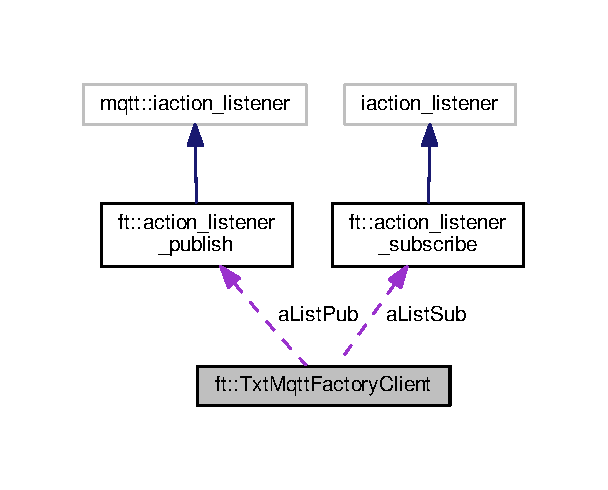
\includegraphics[width=292pt]{classft_1_1_txt_mqtt_factory_client__coll__graph}
\end{center}
\end{figure}
\subsection*{Public Member Functions}
\begin{DoxyCompactItemize}
\item 
\hyperlink{classft_1_1_txt_mqtt_factory_client_a31996ffdaa56d4faf1e4e3af3ff13579}{Txt\+Mqtt\+Factory\+Client} (std\+::string \hyperlink{classft_1_1_txt_mqtt_factory_client_a22be9e9d3b627a159aced6ae6bdffcc2}{clientname}, std\+::string \hyperlink{classft_1_1_txt_mqtt_factory_client_aa927ee53f42359598d014b334c064d83}{host}, std\+::string \hyperlink{classft_1_1_txt_mqtt_factory_client_af60c5887f1eae5dc4039fa284eb2b0b6}{port}, std\+::string \hyperlink{classft_1_1_txt_mqtt_factory_client_ab4c4b9312d3df970892ae26c143eb5ff}{mqtt\+\_\+user}, mqtt\+::binary\+\_\+ref \hyperlink{classft_1_1_txt_mqtt_factory_client_abb1d5f2fd93c87710ad4ea57d3d6702b}{mqtt\+\_\+pass}, bool \hyperlink{classft_1_1_txt_mqtt_factory_client_a057a4b3e05359993f4e591dfac65e56a}{bretained}=false, int \hyperlink{classft_1_1_txt_mqtt_factory_client_a63fa34c118f67674e0afb96ca3af1408}{iqos}=1)
\item 
virtual \hyperlink{classft_1_1_txt_mqtt_factory_client_a819f30cbefa3ddd5547e8c88aa78dde3}{$\sim$\+Txt\+Mqtt\+Factory\+Client} ()
\item 
bool \hyperlink{classft_1_1_txt_mqtt_factory_client_ac63f2c42da427fb8d2607f861981fcc1}{is\+\_\+connected} ()
\item 
bool \hyperlink{classft_1_1_txt_mqtt_factory_client_aa0626009466c14b2f7c3b2da276a3c87}{connect} (long int timeout)
\item 
void \hyperlink{classft_1_1_txt_mqtt_factory_client_a7e77bcf793eaee53762244b21b9b4b97}{disconnect} (long int timeout)
\item 
void \hyperlink{classft_1_1_txt_mqtt_factory_client_af31825b5b21a4bab5742eb59407305e7}{set\+\_\+callback} (mqtt\+::callback \&cb)
\item 
bool \hyperlink{classft_1_1_txt_mqtt_factory_client_a6501429911b63950cea973b001f24cf8}{start\+\_\+consume} (long int timeout)
\item 
void \hyperlink{classft_1_1_txt_mqtt_factory_client_ac56473bd135be28aac2caeeff0dd06eb}{publish\+L\+DR} (double timestamp\+\_\+s, int16\+\_\+t ldr, long timeout)
\item 
void \hyperlink{classft_1_1_txt_mqtt_factory_client_ad58fa45acba2c4b7ee208a4efdbf2140}{publish\+Ptu\+Pos} (float pan, float tilt, long timeout)
\item 
void \hyperlink{classft_1_1_txt_mqtt_factory_client_a4a442350cebe528f0fc90dbb2f67c1de}{publish\+Cam} (const std\+::string sdata, long timeout)
\item 
void \hyperlink{classft_1_1_txt_mqtt_factory_client_a225a231a4ec63ef047625e5cd2ec33a2}{publish\+Bme680} (int64\+\_\+t timestamp, float iaq, uint8\+\_\+t iaq\+\_\+accuracy, float temperature, float humidity, float pressure, float raw\+\_\+temperature, float raw\+\_\+humidity, float gas, long timeout)
\item 
void \hyperlink{classft_1_1_txt_mqtt_factory_client_aad1434a675a1ad95bc526747bae82865}{publish\+Alert} (bool st, const std\+::string id, const std\+::string sdata, int code, long timeout)
\item 
void \hyperlink{classft_1_1_txt_mqtt_factory_client_afc7d9b8edcead431fb67c732152b55a1}{publish\+Broadcast} (double timestamp\+\_\+s, const std\+::string sw, const std\+::string ver, const std\+::string message, long timeout)
\item 
void \hyperlink{classft_1_1_txt_mqtt_factory_client_ab53fbf613676b49e98352a6b226ab3d0}{publish\+State\+S\+LD} (\hyperlink{namespaceft_a14147563037506fac6464a9f6bcbad40}{Txt\+L\+E\+D\+S\+Code\+\_\+t} code, const std\+::string desc, long timeout, int active=-\/1, const std\+::string target=\char`\"{}\char`\"{})
\item 
void \hyperlink{classft_1_1_txt_mqtt_factory_client_a856c542e74f14e6a12cca62dd3566401}{publish\+State\+V\+GR} (\hyperlink{namespaceft_a14147563037506fac6464a9f6bcbad40}{Txt\+L\+E\+D\+S\+Code\+\_\+t} code, const std\+::string desc, long timeout, int active=-\/1, const std\+::string target=\char`\"{}\char`\"{})
\item 
void \hyperlink{classft_1_1_txt_mqtt_factory_client_ae68fac9f8874b963b2cf1a4ee9756211}{publish\+State\+D\+SI} (\hyperlink{namespaceft_a14147563037506fac6464a9f6bcbad40}{Txt\+L\+E\+D\+S\+Code\+\_\+t} code, const std\+::string desc, long timeout, int active=-\/1, const std\+::string target=\char`\"{}\char`\"{})
\item 
void \hyperlink{classft_1_1_txt_mqtt_factory_client_a0c083001539aba0ec4cfbe5d98974d8f}{publish\+State\+D\+SO} (\hyperlink{namespaceft_a14147563037506fac6464a9f6bcbad40}{Txt\+L\+E\+D\+S\+Code\+\_\+t} code, const std\+::string desc, long timeout, int active=-\/1, const std\+::string target=\char`\"{}\char`\"{})
\item 
void \hyperlink{classft_1_1_txt_mqtt_factory_client_adc12b60d1c0e4a7fc342a215bb055779}{publish\+State\+M\+PO} (\hyperlink{namespaceft_a14147563037506fac6464a9f6bcbad40}{Txt\+L\+E\+D\+S\+Code\+\_\+t} code, const std\+::string desc, long timeout, int active=-\/1, const std\+::string target=\char`\"{}\char`\"{})
\item 
void \hyperlink{classft_1_1_txt_mqtt_factory_client_a1f3c9b6117088049610042682bc21daa}{publish\+State\+H\+BW} (\hyperlink{namespaceft_a14147563037506fac6464a9f6bcbad40}{Txt\+L\+E\+D\+S\+Code\+\_\+t} code, const std\+::string desc, long timeout, int active=-\/1, const std\+::string target=\char`\"{}\char`\"{})
\item 
void \hyperlink{classft_1_1_txt_mqtt_factory_client_aa379fdca720ae6e258fdab746f22b5f2}{publish\+Stock} (\hyperlink{namespaceft_a3d5e802a7d78dac37b288630c9b21e64}{Stock\+\_\+map\+\_\+t} map\+\_\+wps, long timeout)
\item 
void \hyperlink{classft_1_1_txt_mqtt_factory_client_a10294cf5b852e5d6e24d7456853a3266}{publish\+State\+Order} (\hyperlink{structft_1_1_txt_order_state}{Txt\+Order\+State} ord\+\_\+state, long timeout)
\item 
void \hyperlink{classft_1_1_txt_mqtt_factory_client_a2fdd6b38c083c41c2da9f748a35b24c9}{publish\+Nfc\+DS} (\hyperlink{classft_1_1_txt_workpiece}{Txt\+Workpiece} wp, \hyperlink{namespaceft_aa7740d5a5a633c96d2063e7fd135cf89}{History\+\_\+map\+\_\+t} map\+\_\+hist, long timeout)
\item 
void \hyperlink{classft_1_1_txt_mqtt_factory_client_a1cdb5649368d07e48b05892ea54b812c}{publish\+S\+S\+C\+\_\+\+Joy} (\hyperlink{classft_1_1_txt_joysticks_data}{Txt\+Joysticks\+Data} jd, long timeout)
\item 
void \hyperlink{classft_1_1_txt_mqtt_factory_client_aae063650cf96166e8e7f468dc94af57c}{publish\+M\+P\+O\+\_\+\+Ack} (\hyperlink{namespaceft_a368e4d4d861f00b9f4faa23c052bdb46}{Txt\+Mpo\+Ack\+Code\+\_\+t} code, long timeout)
\item 
void \hyperlink{classft_1_1_txt_mqtt_factory_client_a337e7510ee005d530e78719c167a3f6a}{publish\+V\+G\+R\+\_\+\+Do} (\hyperlink{namespaceft_a91a43ab1445a680e5e113eec631eb030}{Txt\+Vgr\+Do\+Code\+\_\+t} code, \hyperlink{classft_1_1_txt_workpiece}{Txt\+Workpiece} $\ast$wp, long timeout)
\item 
void \hyperlink{classft_1_1_txt_mqtt_factory_client_ab984a39ea8b1145a8e9b0fd2c1061f3b}{publish\+H\+B\+W\+\_\+\+Ack} (\hyperlink{namespaceft_a79f8dea1d67f613a9366fec07e43e2ff}{Txt\+Hbw\+Ack\+Code\+\_\+t} code, \hyperlink{classft_1_1_txt_workpiece}{Txt\+Workpiece} $\ast$wp, long timeout)
\item 
void \hyperlink{classft_1_1_txt_mqtt_factory_client_a39939c7d24103887e27e26256703abd9}{publish\+S\+L\+D\+\_\+\+Ack} (\hyperlink{namespaceft_aee05f9d6ddbc6bb6add8c06f3e4067a0}{Txt\+Sld\+Ack\+Code\+\_\+t} code, \hyperlink{namespaceft_a2d5bf01b2da29de3c061682f3195b5b2}{Txt\+W\+P\+Type\+\_\+t} type, int value, long timeout)
\end{DoxyCompactItemize}
\subsection*{Protected Member Functions}
\begin{DoxyCompactItemize}
\item 
void \hyperlink{classft_1_1_txt_mqtt_factory_client_ad3915dae96da31b0b5abd1446cc899cf}{publish\+State\+Station} (const std\+::string station, \hyperlink{namespaceft_a14147563037506fac6464a9f6bcbad40}{Txt\+L\+E\+D\+S\+Code\+\_\+t} code, const std\+::string desc, long timeout, int active=-\/1, const std\+::string target=\char`\"{}\char`\"{})
\item 
void \hyperlink{classft_1_1_txt_mqtt_factory_client_a10e4e06910bca4e44656d178d3b01080}{sub\+Topic} (const std\+::string \&topic\+Filter, long int timeout)
\item 
void \hyperlink{classft_1_1_txt_mqtt_factory_client_abfd1407dd236dee490108671bb370d8d}{unsub\+Topic} (const std\+::string \&topic\+Filter, long int timeout)
\end{DoxyCompactItemize}
\subsection*{Protected Attributes}
\begin{DoxyCompactItemize}
\item 
std\+::string \hyperlink{classft_1_1_txt_mqtt_factory_client_a22be9e9d3b627a159aced6ae6bdffcc2}{clientname}
\item 
mqtt\+::string \hyperlink{classft_1_1_txt_mqtt_factory_client_aa927ee53f42359598d014b334c064d83}{host}
\item 
mqtt\+::string \hyperlink{classft_1_1_txt_mqtt_factory_client_af60c5887f1eae5dc4039fa284eb2b0b6}{port}
\item 
mqtt\+::string \hyperlink{classft_1_1_txt_mqtt_factory_client_ab4c4b9312d3df970892ae26c143eb5ff}{mqtt\+\_\+user}
\item 
mqtt\+::binary\+\_\+ref \hyperlink{classft_1_1_txt_mqtt_factory_client_abb1d5f2fd93c87710ad4ea57d3d6702b}{mqtt\+\_\+pass}
\item 
bool \hyperlink{classft_1_1_txt_mqtt_factory_client_a057a4b3e05359993f4e591dfac65e56a}{bretained}
\item 
int \hyperlink{classft_1_1_txt_mqtt_factory_client_a63fa34c118f67674e0afb96ca3af1408}{iqos}
\item 
mqtt\+::async\+\_\+client \hyperlink{classft_1_1_txt_mqtt_factory_client_a39b8ca61026e78a31ea72c82964fd2ad}{cli}
\item 
mqtt\+::connect\+\_\+options \hyperlink{classft_1_1_txt_mqtt_factory_client_a39f8ad4996bb34b7acbfd063f8f68a91}{conn\+Opts}
\item 
pthread\+\_\+mutex\+\_\+t \hyperlink{classft_1_1_txt_mqtt_factory_client_adb54c5156c67a8caec9e482e2d1c6e70}{m\+\_\+mutex}
\item 
\hyperlink{classft_1_1action__listener__subscribe}{action\+\_\+listener\+\_\+subscribe} \hyperlink{classft_1_1_txt_mqtt_factory_client_a881a48419f359ee94ee6731e742ffb66}{a\+List\+Sub}
\item 
\hyperlink{classft_1_1action__listener__publish}{action\+\_\+listener\+\_\+publish} \hyperlink{classft_1_1_txt_mqtt_factory_client_ad384e6f4dd23d4470bbf47d2ade13195}{a\+List\+Pub}
\end{DoxyCompactItemize}


\subsection{Constructor \& Destructor Documentation}
\index{ft\+::\+Txt\+Mqtt\+Factory\+Client@{ft\+::\+Txt\+Mqtt\+Factory\+Client}!Txt\+Mqtt\+Factory\+Client@{Txt\+Mqtt\+Factory\+Client}}
\index{Txt\+Mqtt\+Factory\+Client@{Txt\+Mqtt\+Factory\+Client}!ft\+::\+Txt\+Mqtt\+Factory\+Client@{ft\+::\+Txt\+Mqtt\+Factory\+Client}}
\subsubsection[{\texorpdfstring{Txt\+Mqtt\+Factory\+Client(std\+::string clientname, std\+::string host, std\+::string port, std\+::string mqtt\+\_\+user, mqtt\+::binary\+\_\+ref mqtt\+\_\+pass, bool bretained=false, int iqos=1)}{TxtMqttFactoryClient(std::string clientname, std::string host, std::string port, std::string mqtt_user, mqtt::binary_ref mqtt_pass, bool bretained=false, int iqos=1)}}]{\setlength{\rightskip}{0pt plus 5cm}ft\+::\+Txt\+Mqtt\+Factory\+Client\+::\+Txt\+Mqtt\+Factory\+Client (
\begin{DoxyParamCaption}
\item[{std\+::string}]{clientname, }
\item[{std\+::string}]{host, }
\item[{std\+::string}]{port, }
\item[{std\+::string}]{mqtt\+\_\+user, }
\item[{mqtt\+::binary\+\_\+ref}]{mqtt\+\_\+pass, }
\item[{bool}]{bretained = {\ttfamily false}, }
\item[{int}]{iqos = {\ttfamily 1}}
\end{DoxyParamCaption}
)}\hypertarget{classft_1_1_txt_mqtt_factory_client_a31996ffdaa56d4faf1e4e3af3ff13579}{}\label{classft_1_1_txt_mqtt_factory_client_a31996ffdaa56d4faf1e4e3af3ff13579}
\index{ft\+::\+Txt\+Mqtt\+Factory\+Client@{ft\+::\+Txt\+Mqtt\+Factory\+Client}!````~Txt\+Mqtt\+Factory\+Client@{$\sim$\+Txt\+Mqtt\+Factory\+Client}}
\index{````~Txt\+Mqtt\+Factory\+Client@{$\sim$\+Txt\+Mqtt\+Factory\+Client}!ft\+::\+Txt\+Mqtt\+Factory\+Client@{ft\+::\+Txt\+Mqtt\+Factory\+Client}}
\subsubsection[{\texorpdfstring{$\sim$\+Txt\+Mqtt\+Factory\+Client()}{~TxtMqttFactoryClient()}}]{\setlength{\rightskip}{0pt plus 5cm}virtual ft\+::\+Txt\+Mqtt\+Factory\+Client\+::$\sim$\+Txt\+Mqtt\+Factory\+Client (
\begin{DoxyParamCaption}
{}
\end{DoxyParamCaption}
)\hspace{0.3cm}{\ttfamily [virtual]}}\hypertarget{classft_1_1_txt_mqtt_factory_client_a819f30cbefa3ddd5547e8c88aa78dde3}{}\label{classft_1_1_txt_mqtt_factory_client_a819f30cbefa3ddd5547e8c88aa78dde3}


\subsection{Member Function Documentation}
\index{ft\+::\+Txt\+Mqtt\+Factory\+Client@{ft\+::\+Txt\+Mqtt\+Factory\+Client}!connect@{connect}}
\index{connect@{connect}!ft\+::\+Txt\+Mqtt\+Factory\+Client@{ft\+::\+Txt\+Mqtt\+Factory\+Client}}
\subsubsection[{\texorpdfstring{connect(long int timeout)}{connect(long int timeout)}}]{\setlength{\rightskip}{0pt plus 5cm}bool ft\+::\+Txt\+Mqtt\+Factory\+Client\+::connect (
\begin{DoxyParamCaption}
\item[{long int}]{timeout}
\end{DoxyParamCaption}
)}\hypertarget{classft_1_1_txt_mqtt_factory_client_aa0626009466c14b2f7c3b2da276a3c87}{}\label{classft_1_1_txt_mqtt_factory_client_aa0626009466c14b2f7c3b2da276a3c87}
\index{ft\+::\+Txt\+Mqtt\+Factory\+Client@{ft\+::\+Txt\+Mqtt\+Factory\+Client}!disconnect@{disconnect}}
\index{disconnect@{disconnect}!ft\+::\+Txt\+Mqtt\+Factory\+Client@{ft\+::\+Txt\+Mqtt\+Factory\+Client}}
\subsubsection[{\texorpdfstring{disconnect(long int timeout)}{disconnect(long int timeout)}}]{\setlength{\rightskip}{0pt plus 5cm}void ft\+::\+Txt\+Mqtt\+Factory\+Client\+::disconnect (
\begin{DoxyParamCaption}
\item[{long int}]{timeout}
\end{DoxyParamCaption}
)}\hypertarget{classft_1_1_txt_mqtt_factory_client_a7e77bcf793eaee53762244b21b9b4b97}{}\label{classft_1_1_txt_mqtt_factory_client_a7e77bcf793eaee53762244b21b9b4b97}
\index{ft\+::\+Txt\+Mqtt\+Factory\+Client@{ft\+::\+Txt\+Mqtt\+Factory\+Client}!is\+\_\+connected@{is\+\_\+connected}}
\index{is\+\_\+connected@{is\+\_\+connected}!ft\+::\+Txt\+Mqtt\+Factory\+Client@{ft\+::\+Txt\+Mqtt\+Factory\+Client}}
\subsubsection[{\texorpdfstring{is\+\_\+connected()}{is_connected()}}]{\setlength{\rightskip}{0pt plus 5cm}bool ft\+::\+Txt\+Mqtt\+Factory\+Client\+::is\+\_\+connected (
\begin{DoxyParamCaption}
{}
\end{DoxyParamCaption}
)\hspace{0.3cm}{\ttfamily [inline]}}\hypertarget{classft_1_1_txt_mqtt_factory_client_ac63f2c42da427fb8d2607f861981fcc1}{}\label{classft_1_1_txt_mqtt_factory_client_ac63f2c42da427fb8d2607f861981fcc1}
\index{ft\+::\+Txt\+Mqtt\+Factory\+Client@{ft\+::\+Txt\+Mqtt\+Factory\+Client}!publish\+Alert@{publish\+Alert}}
\index{publish\+Alert@{publish\+Alert}!ft\+::\+Txt\+Mqtt\+Factory\+Client@{ft\+::\+Txt\+Mqtt\+Factory\+Client}}
\subsubsection[{\texorpdfstring{publish\+Alert(bool st, const std\+::string id, const std\+::string sdata, int code, long timeout)}{publishAlert(bool st, const std::string id, const std::string sdata, int code, long timeout)}}]{\setlength{\rightskip}{0pt plus 5cm}void ft\+::\+Txt\+Mqtt\+Factory\+Client\+::publish\+Alert (
\begin{DoxyParamCaption}
\item[{bool}]{st, }
\item[{const std\+::string}]{id, }
\item[{const std\+::string}]{sdata, }
\item[{int}]{code, }
\item[{long}]{timeout}
\end{DoxyParamCaption}
)}\hypertarget{classft_1_1_txt_mqtt_factory_client_aad1434a675a1ad95bc526747bae82865}{}\label{classft_1_1_txt_mqtt_factory_client_aad1434a675a1ad95bc526747bae82865}
\index{ft\+::\+Txt\+Mqtt\+Factory\+Client@{ft\+::\+Txt\+Mqtt\+Factory\+Client}!publish\+Bme680@{publish\+Bme680}}
\index{publish\+Bme680@{publish\+Bme680}!ft\+::\+Txt\+Mqtt\+Factory\+Client@{ft\+::\+Txt\+Mqtt\+Factory\+Client}}
\subsubsection[{\texorpdfstring{publish\+Bme680(int64\+\_\+t timestamp, float iaq, uint8\+\_\+t iaq\+\_\+accuracy, float temperature, float humidity, float pressure, float raw\+\_\+temperature, float raw\+\_\+humidity, float gas, long timeout)}{publishBme680(int64_t timestamp, float iaq, uint8_t iaq_accuracy, float temperature, float humidity, float pressure, float raw_temperature, float raw_humidity, float gas, long timeout)}}]{\setlength{\rightskip}{0pt plus 5cm}void ft\+::\+Txt\+Mqtt\+Factory\+Client\+::publish\+Bme680 (
\begin{DoxyParamCaption}
\item[{int64\+\_\+t}]{timestamp, }
\item[{float}]{iaq, }
\item[{uint8\+\_\+t}]{iaq\+\_\+accuracy, }
\item[{float}]{temperature, }
\item[{float}]{humidity, }
\item[{float}]{pressure, }
\item[{float}]{raw\+\_\+temperature, }
\item[{float}]{raw\+\_\+humidity, }
\item[{float}]{gas, }
\item[{long}]{timeout}
\end{DoxyParamCaption}
)}\hypertarget{classft_1_1_txt_mqtt_factory_client_a225a231a4ec63ef047625e5cd2ec33a2}{}\label{classft_1_1_txt_mqtt_factory_client_a225a231a4ec63ef047625e5cd2ec33a2}
\index{ft\+::\+Txt\+Mqtt\+Factory\+Client@{ft\+::\+Txt\+Mqtt\+Factory\+Client}!publish\+Broadcast@{publish\+Broadcast}}
\index{publish\+Broadcast@{publish\+Broadcast}!ft\+::\+Txt\+Mqtt\+Factory\+Client@{ft\+::\+Txt\+Mqtt\+Factory\+Client}}
\subsubsection[{\texorpdfstring{publish\+Broadcast(double timestamp\+\_\+s, const std\+::string sw, const std\+::string ver, const std\+::string message, long timeout)}{publishBroadcast(double timestamp_s, const std::string sw, const std::string ver, const std::string message, long timeout)}}]{\setlength{\rightskip}{0pt plus 5cm}void ft\+::\+Txt\+Mqtt\+Factory\+Client\+::publish\+Broadcast (
\begin{DoxyParamCaption}
\item[{double}]{timestamp\+\_\+s, }
\item[{const std\+::string}]{sw, }
\item[{const std\+::string}]{ver, }
\item[{const std\+::string}]{message, }
\item[{long}]{timeout}
\end{DoxyParamCaption}
)}\hypertarget{classft_1_1_txt_mqtt_factory_client_afc7d9b8edcead431fb67c732152b55a1}{}\label{classft_1_1_txt_mqtt_factory_client_afc7d9b8edcead431fb67c732152b55a1}
\index{ft\+::\+Txt\+Mqtt\+Factory\+Client@{ft\+::\+Txt\+Mqtt\+Factory\+Client}!publish\+Cam@{publish\+Cam}}
\index{publish\+Cam@{publish\+Cam}!ft\+::\+Txt\+Mqtt\+Factory\+Client@{ft\+::\+Txt\+Mqtt\+Factory\+Client}}
\subsubsection[{\texorpdfstring{publish\+Cam(const std\+::string sdata, long timeout)}{publishCam(const std::string sdata, long timeout)}}]{\setlength{\rightskip}{0pt plus 5cm}void ft\+::\+Txt\+Mqtt\+Factory\+Client\+::publish\+Cam (
\begin{DoxyParamCaption}
\item[{const std\+::string}]{sdata, }
\item[{long}]{timeout}
\end{DoxyParamCaption}
)}\hypertarget{classft_1_1_txt_mqtt_factory_client_a4a442350cebe528f0fc90dbb2f67c1de}{}\label{classft_1_1_txt_mqtt_factory_client_a4a442350cebe528f0fc90dbb2f67c1de}
\index{ft\+::\+Txt\+Mqtt\+Factory\+Client@{ft\+::\+Txt\+Mqtt\+Factory\+Client}!publish\+H\+B\+W\+\_\+\+Ack@{publish\+H\+B\+W\+\_\+\+Ack}}
\index{publish\+H\+B\+W\+\_\+\+Ack@{publish\+H\+B\+W\+\_\+\+Ack}!ft\+::\+Txt\+Mqtt\+Factory\+Client@{ft\+::\+Txt\+Mqtt\+Factory\+Client}}
\subsubsection[{\texorpdfstring{publish\+H\+B\+W\+\_\+\+Ack(\+Txt\+Hbw\+Ack\+Code\+\_\+t code, Txt\+Workpiece $\ast$wp, long timeout)}{publishHBW_Ack(TxtHbwAckCode_t code, TxtWorkpiece *wp, long timeout)}}]{\setlength{\rightskip}{0pt plus 5cm}void ft\+::\+Txt\+Mqtt\+Factory\+Client\+::publish\+H\+B\+W\+\_\+\+Ack (
\begin{DoxyParamCaption}
\item[{{\bf Txt\+Hbw\+Ack\+Code\+\_\+t}}]{code, }
\item[{{\bf Txt\+Workpiece} $\ast$}]{wp, }
\item[{long}]{timeout}
\end{DoxyParamCaption}
)}\hypertarget{classft_1_1_txt_mqtt_factory_client_ab984a39ea8b1145a8e9b0fd2c1061f3b}{}\label{classft_1_1_txt_mqtt_factory_client_ab984a39ea8b1145a8e9b0fd2c1061f3b}
\index{ft\+::\+Txt\+Mqtt\+Factory\+Client@{ft\+::\+Txt\+Mqtt\+Factory\+Client}!publish\+L\+DR@{publish\+L\+DR}}
\index{publish\+L\+DR@{publish\+L\+DR}!ft\+::\+Txt\+Mqtt\+Factory\+Client@{ft\+::\+Txt\+Mqtt\+Factory\+Client}}
\subsubsection[{\texorpdfstring{publish\+L\+D\+R(double timestamp\+\_\+s, int16\+\_\+t ldr, long timeout)}{publishLDR(double timestamp_s, int16_t ldr, long timeout)}}]{\setlength{\rightskip}{0pt plus 5cm}void ft\+::\+Txt\+Mqtt\+Factory\+Client\+::publish\+L\+DR (
\begin{DoxyParamCaption}
\item[{double}]{timestamp\+\_\+s, }
\item[{int16\+\_\+t}]{ldr, }
\item[{long}]{timeout}
\end{DoxyParamCaption}
)}\hypertarget{classft_1_1_txt_mqtt_factory_client_ac56473bd135be28aac2caeeff0dd06eb}{}\label{classft_1_1_txt_mqtt_factory_client_ac56473bd135be28aac2caeeff0dd06eb}
\index{ft\+::\+Txt\+Mqtt\+Factory\+Client@{ft\+::\+Txt\+Mqtt\+Factory\+Client}!publish\+M\+P\+O\+\_\+\+Ack@{publish\+M\+P\+O\+\_\+\+Ack}}
\index{publish\+M\+P\+O\+\_\+\+Ack@{publish\+M\+P\+O\+\_\+\+Ack}!ft\+::\+Txt\+Mqtt\+Factory\+Client@{ft\+::\+Txt\+Mqtt\+Factory\+Client}}
\subsubsection[{\texorpdfstring{publish\+M\+P\+O\+\_\+\+Ack(\+Txt\+Mpo\+Ack\+Code\+\_\+t code, long timeout)}{publishMPO_Ack(TxtMpoAckCode_t code, long timeout)}}]{\setlength{\rightskip}{0pt plus 5cm}void ft\+::\+Txt\+Mqtt\+Factory\+Client\+::publish\+M\+P\+O\+\_\+\+Ack (
\begin{DoxyParamCaption}
\item[{{\bf Txt\+Mpo\+Ack\+Code\+\_\+t}}]{code, }
\item[{long}]{timeout}
\end{DoxyParamCaption}
)}\hypertarget{classft_1_1_txt_mqtt_factory_client_aae063650cf96166e8e7f468dc94af57c}{}\label{classft_1_1_txt_mqtt_factory_client_aae063650cf96166e8e7f468dc94af57c}
\index{ft\+::\+Txt\+Mqtt\+Factory\+Client@{ft\+::\+Txt\+Mqtt\+Factory\+Client}!publish\+Nfc\+DS@{publish\+Nfc\+DS}}
\index{publish\+Nfc\+DS@{publish\+Nfc\+DS}!ft\+::\+Txt\+Mqtt\+Factory\+Client@{ft\+::\+Txt\+Mqtt\+Factory\+Client}}
\subsubsection[{\texorpdfstring{publish\+Nfc\+D\+S(\+Txt\+Workpiece wp, History\+\_\+map\+\_\+t map\+\_\+hist, long timeout)}{publishNfcDS(TxtWorkpiece wp, History_map_t map_hist, long timeout)}}]{\setlength{\rightskip}{0pt plus 5cm}void ft\+::\+Txt\+Mqtt\+Factory\+Client\+::publish\+Nfc\+DS (
\begin{DoxyParamCaption}
\item[{{\bf Txt\+Workpiece}}]{wp, }
\item[{{\bf History\+\_\+map\+\_\+t}}]{map\+\_\+hist, }
\item[{long}]{timeout}
\end{DoxyParamCaption}
)}\hypertarget{classft_1_1_txt_mqtt_factory_client_a2fdd6b38c083c41c2da9f748a35b24c9}{}\label{classft_1_1_txt_mqtt_factory_client_a2fdd6b38c083c41c2da9f748a35b24c9}
\index{ft\+::\+Txt\+Mqtt\+Factory\+Client@{ft\+::\+Txt\+Mqtt\+Factory\+Client}!publish\+Ptu\+Pos@{publish\+Ptu\+Pos}}
\index{publish\+Ptu\+Pos@{publish\+Ptu\+Pos}!ft\+::\+Txt\+Mqtt\+Factory\+Client@{ft\+::\+Txt\+Mqtt\+Factory\+Client}}
\subsubsection[{\texorpdfstring{publish\+Ptu\+Pos(float pan, float tilt, long timeout)}{publishPtuPos(float pan, float tilt, long timeout)}}]{\setlength{\rightskip}{0pt plus 5cm}void ft\+::\+Txt\+Mqtt\+Factory\+Client\+::publish\+Ptu\+Pos (
\begin{DoxyParamCaption}
\item[{float}]{pan, }
\item[{float}]{tilt, }
\item[{long}]{timeout}
\end{DoxyParamCaption}
)}\hypertarget{classft_1_1_txt_mqtt_factory_client_ad58fa45acba2c4b7ee208a4efdbf2140}{}\label{classft_1_1_txt_mqtt_factory_client_ad58fa45acba2c4b7ee208a4efdbf2140}
\index{ft\+::\+Txt\+Mqtt\+Factory\+Client@{ft\+::\+Txt\+Mqtt\+Factory\+Client}!publish\+S\+L\+D\+\_\+\+Ack@{publish\+S\+L\+D\+\_\+\+Ack}}
\index{publish\+S\+L\+D\+\_\+\+Ack@{publish\+S\+L\+D\+\_\+\+Ack}!ft\+::\+Txt\+Mqtt\+Factory\+Client@{ft\+::\+Txt\+Mqtt\+Factory\+Client}}
\subsubsection[{\texorpdfstring{publish\+S\+L\+D\+\_\+\+Ack(\+Txt\+Sld\+Ack\+Code\+\_\+t code, Txt\+W\+P\+Type\+\_\+t type, int value, long timeout)}{publishSLD_Ack(TxtSldAckCode_t code, TxtWPType_t type, int value, long timeout)}}]{\setlength{\rightskip}{0pt plus 5cm}void ft\+::\+Txt\+Mqtt\+Factory\+Client\+::publish\+S\+L\+D\+\_\+\+Ack (
\begin{DoxyParamCaption}
\item[{{\bf Txt\+Sld\+Ack\+Code\+\_\+t}}]{code, }
\item[{{\bf Txt\+W\+P\+Type\+\_\+t}}]{type, }
\item[{int}]{value, }
\item[{long}]{timeout}
\end{DoxyParamCaption}
)}\hypertarget{classft_1_1_txt_mqtt_factory_client_a39939c7d24103887e27e26256703abd9}{}\label{classft_1_1_txt_mqtt_factory_client_a39939c7d24103887e27e26256703abd9}
\index{ft\+::\+Txt\+Mqtt\+Factory\+Client@{ft\+::\+Txt\+Mqtt\+Factory\+Client}!publish\+S\+S\+C\+\_\+\+Joy@{publish\+S\+S\+C\+\_\+\+Joy}}
\index{publish\+S\+S\+C\+\_\+\+Joy@{publish\+S\+S\+C\+\_\+\+Joy}!ft\+::\+Txt\+Mqtt\+Factory\+Client@{ft\+::\+Txt\+Mqtt\+Factory\+Client}}
\subsubsection[{\texorpdfstring{publish\+S\+S\+C\+\_\+\+Joy(\+Txt\+Joysticks\+Data jd, long timeout)}{publishSSC_Joy(TxtJoysticksData jd, long timeout)}}]{\setlength{\rightskip}{0pt plus 5cm}void ft\+::\+Txt\+Mqtt\+Factory\+Client\+::publish\+S\+S\+C\+\_\+\+Joy (
\begin{DoxyParamCaption}
\item[{{\bf Txt\+Joysticks\+Data}}]{jd, }
\item[{long}]{timeout}
\end{DoxyParamCaption}
)}\hypertarget{classft_1_1_txt_mqtt_factory_client_a1cdb5649368d07e48b05892ea54b812c}{}\label{classft_1_1_txt_mqtt_factory_client_a1cdb5649368d07e48b05892ea54b812c}
\index{ft\+::\+Txt\+Mqtt\+Factory\+Client@{ft\+::\+Txt\+Mqtt\+Factory\+Client}!publish\+State\+D\+SI@{publish\+State\+D\+SI}}
\index{publish\+State\+D\+SI@{publish\+State\+D\+SI}!ft\+::\+Txt\+Mqtt\+Factory\+Client@{ft\+::\+Txt\+Mqtt\+Factory\+Client}}
\subsubsection[{\texorpdfstring{publish\+State\+D\+S\+I(\+Txt\+L\+E\+D\+S\+Code\+\_\+t code, const std\+::string desc, long timeout, int active=-\/1, const std\+::string target="""")}{publishStateDSI(TxtLEDSCode_t code, const std::string desc, long timeout, int active=-1, const std::string target="")}}]{\setlength{\rightskip}{0pt plus 5cm}void ft\+::\+Txt\+Mqtt\+Factory\+Client\+::publish\+State\+D\+SI (
\begin{DoxyParamCaption}
\item[{{\bf Txt\+L\+E\+D\+S\+Code\+\_\+t}}]{code, }
\item[{const std\+::string}]{desc, }
\item[{long}]{timeout, }
\item[{int}]{active = {\ttfamily -\/1}, }
\item[{const std\+::string}]{target = {\ttfamily \char`\"{}\char`\"{}}}
\end{DoxyParamCaption}
)\hspace{0.3cm}{\ttfamily [inline]}}\hypertarget{classft_1_1_txt_mqtt_factory_client_ae68fac9f8874b963b2cf1a4ee9756211}{}\label{classft_1_1_txt_mqtt_factory_client_ae68fac9f8874b963b2cf1a4ee9756211}
\index{ft\+::\+Txt\+Mqtt\+Factory\+Client@{ft\+::\+Txt\+Mqtt\+Factory\+Client}!publish\+State\+D\+SO@{publish\+State\+D\+SO}}
\index{publish\+State\+D\+SO@{publish\+State\+D\+SO}!ft\+::\+Txt\+Mqtt\+Factory\+Client@{ft\+::\+Txt\+Mqtt\+Factory\+Client}}
\subsubsection[{\texorpdfstring{publish\+State\+D\+S\+O(\+Txt\+L\+E\+D\+S\+Code\+\_\+t code, const std\+::string desc, long timeout, int active=-\/1, const std\+::string target="""")}{publishStateDSO(TxtLEDSCode_t code, const std::string desc, long timeout, int active=-1, const std::string target="")}}]{\setlength{\rightskip}{0pt plus 5cm}void ft\+::\+Txt\+Mqtt\+Factory\+Client\+::publish\+State\+D\+SO (
\begin{DoxyParamCaption}
\item[{{\bf Txt\+L\+E\+D\+S\+Code\+\_\+t}}]{code, }
\item[{const std\+::string}]{desc, }
\item[{long}]{timeout, }
\item[{int}]{active = {\ttfamily -\/1}, }
\item[{const std\+::string}]{target = {\ttfamily \char`\"{}\char`\"{}}}
\end{DoxyParamCaption}
)\hspace{0.3cm}{\ttfamily [inline]}}\hypertarget{classft_1_1_txt_mqtt_factory_client_a0c083001539aba0ec4cfbe5d98974d8f}{}\label{classft_1_1_txt_mqtt_factory_client_a0c083001539aba0ec4cfbe5d98974d8f}
\index{ft\+::\+Txt\+Mqtt\+Factory\+Client@{ft\+::\+Txt\+Mqtt\+Factory\+Client}!publish\+State\+H\+BW@{publish\+State\+H\+BW}}
\index{publish\+State\+H\+BW@{publish\+State\+H\+BW}!ft\+::\+Txt\+Mqtt\+Factory\+Client@{ft\+::\+Txt\+Mqtt\+Factory\+Client}}
\subsubsection[{\texorpdfstring{publish\+State\+H\+B\+W(\+Txt\+L\+E\+D\+S\+Code\+\_\+t code, const std\+::string desc, long timeout, int active=-\/1, const std\+::string target="""")}{publishStateHBW(TxtLEDSCode_t code, const std::string desc, long timeout, int active=-1, const std::string target="")}}]{\setlength{\rightskip}{0pt plus 5cm}void ft\+::\+Txt\+Mqtt\+Factory\+Client\+::publish\+State\+H\+BW (
\begin{DoxyParamCaption}
\item[{{\bf Txt\+L\+E\+D\+S\+Code\+\_\+t}}]{code, }
\item[{const std\+::string}]{desc, }
\item[{long}]{timeout, }
\item[{int}]{active = {\ttfamily -\/1}, }
\item[{const std\+::string}]{target = {\ttfamily \char`\"{}\char`\"{}}}
\end{DoxyParamCaption}
)\hspace{0.3cm}{\ttfamily [inline]}}\hypertarget{classft_1_1_txt_mqtt_factory_client_a1f3c9b6117088049610042682bc21daa}{}\label{classft_1_1_txt_mqtt_factory_client_a1f3c9b6117088049610042682bc21daa}
\index{ft\+::\+Txt\+Mqtt\+Factory\+Client@{ft\+::\+Txt\+Mqtt\+Factory\+Client}!publish\+State\+M\+PO@{publish\+State\+M\+PO}}
\index{publish\+State\+M\+PO@{publish\+State\+M\+PO}!ft\+::\+Txt\+Mqtt\+Factory\+Client@{ft\+::\+Txt\+Mqtt\+Factory\+Client}}
\subsubsection[{\texorpdfstring{publish\+State\+M\+P\+O(\+Txt\+L\+E\+D\+S\+Code\+\_\+t code, const std\+::string desc, long timeout, int active=-\/1, const std\+::string target="""")}{publishStateMPO(TxtLEDSCode_t code, const std::string desc, long timeout, int active=-1, const std::string target="")}}]{\setlength{\rightskip}{0pt plus 5cm}void ft\+::\+Txt\+Mqtt\+Factory\+Client\+::publish\+State\+M\+PO (
\begin{DoxyParamCaption}
\item[{{\bf Txt\+L\+E\+D\+S\+Code\+\_\+t}}]{code, }
\item[{const std\+::string}]{desc, }
\item[{long}]{timeout, }
\item[{int}]{active = {\ttfamily -\/1}, }
\item[{const std\+::string}]{target = {\ttfamily \char`\"{}\char`\"{}}}
\end{DoxyParamCaption}
)\hspace{0.3cm}{\ttfamily [inline]}}\hypertarget{classft_1_1_txt_mqtt_factory_client_adc12b60d1c0e4a7fc342a215bb055779}{}\label{classft_1_1_txt_mqtt_factory_client_adc12b60d1c0e4a7fc342a215bb055779}
\index{ft\+::\+Txt\+Mqtt\+Factory\+Client@{ft\+::\+Txt\+Mqtt\+Factory\+Client}!publish\+State\+Order@{publish\+State\+Order}}
\index{publish\+State\+Order@{publish\+State\+Order}!ft\+::\+Txt\+Mqtt\+Factory\+Client@{ft\+::\+Txt\+Mqtt\+Factory\+Client}}
\subsubsection[{\texorpdfstring{publish\+State\+Order(\+Txt\+Order\+State ord\+\_\+state, long timeout)}{publishStateOrder(TxtOrderState ord_state, long timeout)}}]{\setlength{\rightskip}{0pt plus 5cm}void ft\+::\+Txt\+Mqtt\+Factory\+Client\+::publish\+State\+Order (
\begin{DoxyParamCaption}
\item[{{\bf Txt\+Order\+State}}]{ord\+\_\+state, }
\item[{long}]{timeout}
\end{DoxyParamCaption}
)}\hypertarget{classft_1_1_txt_mqtt_factory_client_a10294cf5b852e5d6e24d7456853a3266}{}\label{classft_1_1_txt_mqtt_factory_client_a10294cf5b852e5d6e24d7456853a3266}
\index{ft\+::\+Txt\+Mqtt\+Factory\+Client@{ft\+::\+Txt\+Mqtt\+Factory\+Client}!publish\+State\+S\+LD@{publish\+State\+S\+LD}}
\index{publish\+State\+S\+LD@{publish\+State\+S\+LD}!ft\+::\+Txt\+Mqtt\+Factory\+Client@{ft\+::\+Txt\+Mqtt\+Factory\+Client}}
\subsubsection[{\texorpdfstring{publish\+State\+S\+L\+D(\+Txt\+L\+E\+D\+S\+Code\+\_\+t code, const std\+::string desc, long timeout, int active=-\/1, const std\+::string target="""")}{publishStateSLD(TxtLEDSCode_t code, const std::string desc, long timeout, int active=-1, const std::string target="")}}]{\setlength{\rightskip}{0pt plus 5cm}void ft\+::\+Txt\+Mqtt\+Factory\+Client\+::publish\+State\+S\+LD (
\begin{DoxyParamCaption}
\item[{{\bf Txt\+L\+E\+D\+S\+Code\+\_\+t}}]{code, }
\item[{const std\+::string}]{desc, }
\item[{long}]{timeout, }
\item[{int}]{active = {\ttfamily -\/1}, }
\item[{const std\+::string}]{target = {\ttfamily \char`\"{}\char`\"{}}}
\end{DoxyParamCaption}
)\hspace{0.3cm}{\ttfamily [inline]}}\hypertarget{classft_1_1_txt_mqtt_factory_client_ab53fbf613676b49e98352a6b226ab3d0}{}\label{classft_1_1_txt_mqtt_factory_client_ab53fbf613676b49e98352a6b226ab3d0}
\index{ft\+::\+Txt\+Mqtt\+Factory\+Client@{ft\+::\+Txt\+Mqtt\+Factory\+Client}!publish\+State\+Station@{publish\+State\+Station}}
\index{publish\+State\+Station@{publish\+State\+Station}!ft\+::\+Txt\+Mqtt\+Factory\+Client@{ft\+::\+Txt\+Mqtt\+Factory\+Client}}
\subsubsection[{\texorpdfstring{publish\+State\+Station(const std\+::string station, Txt\+L\+E\+D\+S\+Code\+\_\+t code, const std\+::string desc, long timeout, int active=-\/1, const std\+::string target="""")}{publishStateStation(const std::string station, TxtLEDSCode_t code, const std::string desc, long timeout, int active=-1, const std::string target="")}}]{\setlength{\rightskip}{0pt plus 5cm}void ft\+::\+Txt\+Mqtt\+Factory\+Client\+::publish\+State\+Station (
\begin{DoxyParamCaption}
\item[{const std\+::string}]{station, }
\item[{{\bf Txt\+L\+E\+D\+S\+Code\+\_\+t}}]{code, }
\item[{const std\+::string}]{desc, }
\item[{long}]{timeout, }
\item[{int}]{active = {\ttfamily -\/1}, }
\item[{const std\+::string}]{target = {\ttfamily \char`\"{}\char`\"{}}}
\end{DoxyParamCaption}
)\hspace{0.3cm}{\ttfamily [protected]}}\hypertarget{classft_1_1_txt_mqtt_factory_client_ad3915dae96da31b0b5abd1446cc899cf}{}\label{classft_1_1_txt_mqtt_factory_client_ad3915dae96da31b0b5abd1446cc899cf}
\index{ft\+::\+Txt\+Mqtt\+Factory\+Client@{ft\+::\+Txt\+Mqtt\+Factory\+Client}!publish\+State\+V\+GR@{publish\+State\+V\+GR}}
\index{publish\+State\+V\+GR@{publish\+State\+V\+GR}!ft\+::\+Txt\+Mqtt\+Factory\+Client@{ft\+::\+Txt\+Mqtt\+Factory\+Client}}
\subsubsection[{\texorpdfstring{publish\+State\+V\+G\+R(\+Txt\+L\+E\+D\+S\+Code\+\_\+t code, const std\+::string desc, long timeout, int active=-\/1, const std\+::string target="""")}{publishStateVGR(TxtLEDSCode_t code, const std::string desc, long timeout, int active=-1, const std::string target="")}}]{\setlength{\rightskip}{0pt plus 5cm}void ft\+::\+Txt\+Mqtt\+Factory\+Client\+::publish\+State\+V\+GR (
\begin{DoxyParamCaption}
\item[{{\bf Txt\+L\+E\+D\+S\+Code\+\_\+t}}]{code, }
\item[{const std\+::string}]{desc, }
\item[{long}]{timeout, }
\item[{int}]{active = {\ttfamily -\/1}, }
\item[{const std\+::string}]{target = {\ttfamily \char`\"{}\char`\"{}}}
\end{DoxyParamCaption}
)\hspace{0.3cm}{\ttfamily [inline]}}\hypertarget{classft_1_1_txt_mqtt_factory_client_a856c542e74f14e6a12cca62dd3566401}{}\label{classft_1_1_txt_mqtt_factory_client_a856c542e74f14e6a12cca62dd3566401}
\index{ft\+::\+Txt\+Mqtt\+Factory\+Client@{ft\+::\+Txt\+Mqtt\+Factory\+Client}!publish\+Stock@{publish\+Stock}}
\index{publish\+Stock@{publish\+Stock}!ft\+::\+Txt\+Mqtt\+Factory\+Client@{ft\+::\+Txt\+Mqtt\+Factory\+Client}}
\subsubsection[{\texorpdfstring{publish\+Stock(\+Stock\+\_\+map\+\_\+t map\+\_\+wps, long timeout)}{publishStock(Stock_map_t map_wps, long timeout)}}]{\setlength{\rightskip}{0pt plus 5cm}void ft\+::\+Txt\+Mqtt\+Factory\+Client\+::publish\+Stock (
\begin{DoxyParamCaption}
\item[{{\bf Stock\+\_\+map\+\_\+t}}]{map\+\_\+wps, }
\item[{long}]{timeout}
\end{DoxyParamCaption}
)}\hypertarget{classft_1_1_txt_mqtt_factory_client_aa379fdca720ae6e258fdab746f22b5f2}{}\label{classft_1_1_txt_mqtt_factory_client_aa379fdca720ae6e258fdab746f22b5f2}
\index{ft\+::\+Txt\+Mqtt\+Factory\+Client@{ft\+::\+Txt\+Mqtt\+Factory\+Client}!publish\+V\+G\+R\+\_\+\+Do@{publish\+V\+G\+R\+\_\+\+Do}}
\index{publish\+V\+G\+R\+\_\+\+Do@{publish\+V\+G\+R\+\_\+\+Do}!ft\+::\+Txt\+Mqtt\+Factory\+Client@{ft\+::\+Txt\+Mqtt\+Factory\+Client}}
\subsubsection[{\texorpdfstring{publish\+V\+G\+R\+\_\+\+Do(\+Txt\+Vgr\+Do\+Code\+\_\+t code, Txt\+Workpiece $\ast$wp, long timeout)}{publishVGR_Do(TxtVgrDoCode_t code, TxtWorkpiece *wp, long timeout)}}]{\setlength{\rightskip}{0pt plus 5cm}void ft\+::\+Txt\+Mqtt\+Factory\+Client\+::publish\+V\+G\+R\+\_\+\+Do (
\begin{DoxyParamCaption}
\item[{{\bf Txt\+Vgr\+Do\+Code\+\_\+t}}]{code, }
\item[{{\bf Txt\+Workpiece} $\ast$}]{wp, }
\item[{long}]{timeout}
\end{DoxyParamCaption}
)}\hypertarget{classft_1_1_txt_mqtt_factory_client_a337e7510ee005d530e78719c167a3f6a}{}\label{classft_1_1_txt_mqtt_factory_client_a337e7510ee005d530e78719c167a3f6a}
\index{ft\+::\+Txt\+Mqtt\+Factory\+Client@{ft\+::\+Txt\+Mqtt\+Factory\+Client}!set\+\_\+callback@{set\+\_\+callback}}
\index{set\+\_\+callback@{set\+\_\+callback}!ft\+::\+Txt\+Mqtt\+Factory\+Client@{ft\+::\+Txt\+Mqtt\+Factory\+Client}}
\subsubsection[{\texorpdfstring{set\+\_\+callback(mqtt\+::callback \&cb)}{set_callback(mqtt::callback &cb)}}]{\setlength{\rightskip}{0pt plus 5cm}void ft\+::\+Txt\+Mqtt\+Factory\+Client\+::set\+\_\+callback (
\begin{DoxyParamCaption}
\item[{mqtt\+::callback \&}]{cb}
\end{DoxyParamCaption}
)\hspace{0.3cm}{\ttfamily [inline]}}\hypertarget{classft_1_1_txt_mqtt_factory_client_af31825b5b21a4bab5742eb59407305e7}{}\label{classft_1_1_txt_mqtt_factory_client_af31825b5b21a4bab5742eb59407305e7}
\index{ft\+::\+Txt\+Mqtt\+Factory\+Client@{ft\+::\+Txt\+Mqtt\+Factory\+Client}!start\+\_\+consume@{start\+\_\+consume}}
\index{start\+\_\+consume@{start\+\_\+consume}!ft\+::\+Txt\+Mqtt\+Factory\+Client@{ft\+::\+Txt\+Mqtt\+Factory\+Client}}
\subsubsection[{\texorpdfstring{start\+\_\+consume(long int timeout)}{start_consume(long int timeout)}}]{\setlength{\rightskip}{0pt plus 5cm}bool ft\+::\+Txt\+Mqtt\+Factory\+Client\+::start\+\_\+consume (
\begin{DoxyParamCaption}
\item[{long int}]{timeout}
\end{DoxyParamCaption}
)}\hypertarget{classft_1_1_txt_mqtt_factory_client_a6501429911b63950cea973b001f24cf8}{}\label{classft_1_1_txt_mqtt_factory_client_a6501429911b63950cea973b001f24cf8}
\index{ft\+::\+Txt\+Mqtt\+Factory\+Client@{ft\+::\+Txt\+Mqtt\+Factory\+Client}!sub\+Topic@{sub\+Topic}}
\index{sub\+Topic@{sub\+Topic}!ft\+::\+Txt\+Mqtt\+Factory\+Client@{ft\+::\+Txt\+Mqtt\+Factory\+Client}}
\subsubsection[{\texorpdfstring{sub\+Topic(const std\+::string \&topic\+Filter, long int timeout)}{subTopic(const std::string &topicFilter, long int timeout)}}]{\setlength{\rightskip}{0pt plus 5cm}void ft\+::\+Txt\+Mqtt\+Factory\+Client\+::sub\+Topic (
\begin{DoxyParamCaption}
\item[{const std\+::string \&}]{topic\+Filter, }
\item[{long int}]{timeout}
\end{DoxyParamCaption}
)\hspace{0.3cm}{\ttfamily [protected]}}\hypertarget{classft_1_1_txt_mqtt_factory_client_a10e4e06910bca4e44656d178d3b01080}{}\label{classft_1_1_txt_mqtt_factory_client_a10e4e06910bca4e44656d178d3b01080}
\index{ft\+::\+Txt\+Mqtt\+Factory\+Client@{ft\+::\+Txt\+Mqtt\+Factory\+Client}!unsub\+Topic@{unsub\+Topic}}
\index{unsub\+Topic@{unsub\+Topic}!ft\+::\+Txt\+Mqtt\+Factory\+Client@{ft\+::\+Txt\+Mqtt\+Factory\+Client}}
\subsubsection[{\texorpdfstring{unsub\+Topic(const std\+::string \&topic\+Filter, long int timeout)}{unsubTopic(const std::string &topicFilter, long int timeout)}}]{\setlength{\rightskip}{0pt plus 5cm}void ft\+::\+Txt\+Mqtt\+Factory\+Client\+::unsub\+Topic (
\begin{DoxyParamCaption}
\item[{const std\+::string \&}]{topic\+Filter, }
\item[{long int}]{timeout}
\end{DoxyParamCaption}
)\hspace{0.3cm}{\ttfamily [protected]}}\hypertarget{classft_1_1_txt_mqtt_factory_client_abfd1407dd236dee490108671bb370d8d}{}\label{classft_1_1_txt_mqtt_factory_client_abfd1407dd236dee490108671bb370d8d}


\subsection{Member Data Documentation}
\index{ft\+::\+Txt\+Mqtt\+Factory\+Client@{ft\+::\+Txt\+Mqtt\+Factory\+Client}!a\+List\+Pub@{a\+List\+Pub}}
\index{a\+List\+Pub@{a\+List\+Pub}!ft\+::\+Txt\+Mqtt\+Factory\+Client@{ft\+::\+Txt\+Mqtt\+Factory\+Client}}
\subsubsection[{\texorpdfstring{a\+List\+Pub}{aListPub}}]{\setlength{\rightskip}{0pt plus 5cm}{\bf action\+\_\+listener\+\_\+publish} ft\+::\+Txt\+Mqtt\+Factory\+Client\+::a\+List\+Pub\hspace{0.3cm}{\ttfamily [protected]}}\hypertarget{classft_1_1_txt_mqtt_factory_client_ad384e6f4dd23d4470bbf47d2ade13195}{}\label{classft_1_1_txt_mqtt_factory_client_ad384e6f4dd23d4470bbf47d2ade13195}
\index{ft\+::\+Txt\+Mqtt\+Factory\+Client@{ft\+::\+Txt\+Mqtt\+Factory\+Client}!a\+List\+Sub@{a\+List\+Sub}}
\index{a\+List\+Sub@{a\+List\+Sub}!ft\+::\+Txt\+Mqtt\+Factory\+Client@{ft\+::\+Txt\+Mqtt\+Factory\+Client}}
\subsubsection[{\texorpdfstring{a\+List\+Sub}{aListSub}}]{\setlength{\rightskip}{0pt plus 5cm}{\bf action\+\_\+listener\+\_\+subscribe} ft\+::\+Txt\+Mqtt\+Factory\+Client\+::a\+List\+Sub\hspace{0.3cm}{\ttfamily [protected]}}\hypertarget{classft_1_1_txt_mqtt_factory_client_a881a48419f359ee94ee6731e742ffb66}{}\label{classft_1_1_txt_mqtt_factory_client_a881a48419f359ee94ee6731e742ffb66}
\index{ft\+::\+Txt\+Mqtt\+Factory\+Client@{ft\+::\+Txt\+Mqtt\+Factory\+Client}!bretained@{bretained}}
\index{bretained@{bretained}!ft\+::\+Txt\+Mqtt\+Factory\+Client@{ft\+::\+Txt\+Mqtt\+Factory\+Client}}
\subsubsection[{\texorpdfstring{bretained}{bretained}}]{\setlength{\rightskip}{0pt plus 5cm}bool ft\+::\+Txt\+Mqtt\+Factory\+Client\+::bretained\hspace{0.3cm}{\ttfamily [protected]}}\hypertarget{classft_1_1_txt_mqtt_factory_client_a057a4b3e05359993f4e591dfac65e56a}{}\label{classft_1_1_txt_mqtt_factory_client_a057a4b3e05359993f4e591dfac65e56a}
\index{ft\+::\+Txt\+Mqtt\+Factory\+Client@{ft\+::\+Txt\+Mqtt\+Factory\+Client}!cli@{cli}}
\index{cli@{cli}!ft\+::\+Txt\+Mqtt\+Factory\+Client@{ft\+::\+Txt\+Mqtt\+Factory\+Client}}
\subsubsection[{\texorpdfstring{cli}{cli}}]{\setlength{\rightskip}{0pt plus 5cm}mqtt\+::async\+\_\+client ft\+::\+Txt\+Mqtt\+Factory\+Client\+::cli\hspace{0.3cm}{\ttfamily [protected]}}\hypertarget{classft_1_1_txt_mqtt_factory_client_a39b8ca61026e78a31ea72c82964fd2ad}{}\label{classft_1_1_txt_mqtt_factory_client_a39b8ca61026e78a31ea72c82964fd2ad}
\index{ft\+::\+Txt\+Mqtt\+Factory\+Client@{ft\+::\+Txt\+Mqtt\+Factory\+Client}!clientname@{clientname}}
\index{clientname@{clientname}!ft\+::\+Txt\+Mqtt\+Factory\+Client@{ft\+::\+Txt\+Mqtt\+Factory\+Client}}
\subsubsection[{\texorpdfstring{clientname}{clientname}}]{\setlength{\rightskip}{0pt plus 5cm}std\+::string ft\+::\+Txt\+Mqtt\+Factory\+Client\+::clientname\hspace{0.3cm}{\ttfamily [protected]}}\hypertarget{classft_1_1_txt_mqtt_factory_client_a22be9e9d3b627a159aced6ae6bdffcc2}{}\label{classft_1_1_txt_mqtt_factory_client_a22be9e9d3b627a159aced6ae6bdffcc2}
\index{ft\+::\+Txt\+Mqtt\+Factory\+Client@{ft\+::\+Txt\+Mqtt\+Factory\+Client}!conn\+Opts@{conn\+Opts}}
\index{conn\+Opts@{conn\+Opts}!ft\+::\+Txt\+Mqtt\+Factory\+Client@{ft\+::\+Txt\+Mqtt\+Factory\+Client}}
\subsubsection[{\texorpdfstring{conn\+Opts}{connOpts}}]{\setlength{\rightskip}{0pt plus 5cm}mqtt\+::connect\+\_\+options ft\+::\+Txt\+Mqtt\+Factory\+Client\+::conn\+Opts\hspace{0.3cm}{\ttfamily [protected]}}\hypertarget{classft_1_1_txt_mqtt_factory_client_a39f8ad4996bb34b7acbfd063f8f68a91}{}\label{classft_1_1_txt_mqtt_factory_client_a39f8ad4996bb34b7acbfd063f8f68a91}
\index{ft\+::\+Txt\+Mqtt\+Factory\+Client@{ft\+::\+Txt\+Mqtt\+Factory\+Client}!host@{host}}
\index{host@{host}!ft\+::\+Txt\+Mqtt\+Factory\+Client@{ft\+::\+Txt\+Mqtt\+Factory\+Client}}
\subsubsection[{\texorpdfstring{host}{host}}]{\setlength{\rightskip}{0pt plus 5cm}mqtt\+::string ft\+::\+Txt\+Mqtt\+Factory\+Client\+::host\hspace{0.3cm}{\ttfamily [protected]}}\hypertarget{classft_1_1_txt_mqtt_factory_client_aa927ee53f42359598d014b334c064d83}{}\label{classft_1_1_txt_mqtt_factory_client_aa927ee53f42359598d014b334c064d83}
\index{ft\+::\+Txt\+Mqtt\+Factory\+Client@{ft\+::\+Txt\+Mqtt\+Factory\+Client}!iqos@{iqos}}
\index{iqos@{iqos}!ft\+::\+Txt\+Mqtt\+Factory\+Client@{ft\+::\+Txt\+Mqtt\+Factory\+Client}}
\subsubsection[{\texorpdfstring{iqos}{iqos}}]{\setlength{\rightskip}{0pt plus 5cm}int ft\+::\+Txt\+Mqtt\+Factory\+Client\+::iqos\hspace{0.3cm}{\ttfamily [protected]}}\hypertarget{classft_1_1_txt_mqtt_factory_client_a63fa34c118f67674e0afb96ca3af1408}{}\label{classft_1_1_txt_mqtt_factory_client_a63fa34c118f67674e0afb96ca3af1408}
\index{ft\+::\+Txt\+Mqtt\+Factory\+Client@{ft\+::\+Txt\+Mqtt\+Factory\+Client}!m\+\_\+mutex@{m\+\_\+mutex}}
\index{m\+\_\+mutex@{m\+\_\+mutex}!ft\+::\+Txt\+Mqtt\+Factory\+Client@{ft\+::\+Txt\+Mqtt\+Factory\+Client}}
\subsubsection[{\texorpdfstring{m\+\_\+mutex}{m_mutex}}]{\setlength{\rightskip}{0pt plus 5cm}pthread\+\_\+mutex\+\_\+t ft\+::\+Txt\+Mqtt\+Factory\+Client\+::m\+\_\+mutex\hspace{0.3cm}{\ttfamily [protected]}}\hypertarget{classft_1_1_txt_mqtt_factory_client_adb54c5156c67a8caec9e482e2d1c6e70}{}\label{classft_1_1_txt_mqtt_factory_client_adb54c5156c67a8caec9e482e2d1c6e70}
\index{ft\+::\+Txt\+Mqtt\+Factory\+Client@{ft\+::\+Txt\+Mqtt\+Factory\+Client}!mqtt\+\_\+pass@{mqtt\+\_\+pass}}
\index{mqtt\+\_\+pass@{mqtt\+\_\+pass}!ft\+::\+Txt\+Mqtt\+Factory\+Client@{ft\+::\+Txt\+Mqtt\+Factory\+Client}}
\subsubsection[{\texorpdfstring{mqtt\+\_\+pass}{mqtt_pass}}]{\setlength{\rightskip}{0pt plus 5cm}mqtt\+::binary\+\_\+ref ft\+::\+Txt\+Mqtt\+Factory\+Client\+::mqtt\+\_\+pass\hspace{0.3cm}{\ttfamily [protected]}}\hypertarget{classft_1_1_txt_mqtt_factory_client_abb1d5f2fd93c87710ad4ea57d3d6702b}{}\label{classft_1_1_txt_mqtt_factory_client_abb1d5f2fd93c87710ad4ea57d3d6702b}
\index{ft\+::\+Txt\+Mqtt\+Factory\+Client@{ft\+::\+Txt\+Mqtt\+Factory\+Client}!mqtt\+\_\+user@{mqtt\+\_\+user}}
\index{mqtt\+\_\+user@{mqtt\+\_\+user}!ft\+::\+Txt\+Mqtt\+Factory\+Client@{ft\+::\+Txt\+Mqtt\+Factory\+Client}}
\subsubsection[{\texorpdfstring{mqtt\+\_\+user}{mqtt_user}}]{\setlength{\rightskip}{0pt plus 5cm}mqtt\+::string ft\+::\+Txt\+Mqtt\+Factory\+Client\+::mqtt\+\_\+user\hspace{0.3cm}{\ttfamily [protected]}}\hypertarget{classft_1_1_txt_mqtt_factory_client_ab4c4b9312d3df970892ae26c143eb5ff}{}\label{classft_1_1_txt_mqtt_factory_client_ab4c4b9312d3df970892ae26c143eb5ff}
\index{ft\+::\+Txt\+Mqtt\+Factory\+Client@{ft\+::\+Txt\+Mqtt\+Factory\+Client}!port@{port}}
\index{port@{port}!ft\+::\+Txt\+Mqtt\+Factory\+Client@{ft\+::\+Txt\+Mqtt\+Factory\+Client}}
\subsubsection[{\texorpdfstring{port}{port}}]{\setlength{\rightskip}{0pt plus 5cm}mqtt\+::string ft\+::\+Txt\+Mqtt\+Factory\+Client\+::port\hspace{0.3cm}{\ttfamily [protected]}}\hypertarget{classft_1_1_txt_mqtt_factory_client_af60c5887f1eae5dc4039fa284eb2b0b6}{}\label{classft_1_1_txt_mqtt_factory_client_af60c5887f1eae5dc4039fa284eb2b0b6}


The documentation for this class was generated from the following file\+:\begin{DoxyCompactItemize}
\item 
\hyperlink{_txt_mqtt_factory_client_8h}{Txt\+Mqtt\+Factory\+Client.\+h}\end{DoxyCompactItemize}

\hypertarget{classft_1_1_txt_multi_processing_station}{}\section{ft\+:\+:Txt\+Multi\+Processing\+Station Class Reference}
\label{classft_1_1_txt_multi_processing_station}\index{ft\+::\+Txt\+Multi\+Processing\+Station@{ft\+::\+Txt\+Multi\+Processing\+Station}}


{\ttfamily \#include $<$Txt\+Multi\+Processing\+Station.\+h$>$}



Inheritance diagram for ft\+:\+:Txt\+Multi\+Processing\+Station\+:
\nopagebreak
\begin{figure}[H]
\begin{center}
\leavevmode
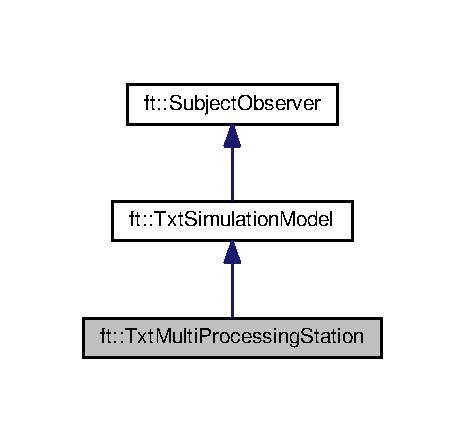
\includegraphics[width=223pt]{classft_1_1_txt_multi_processing_station__inherit__graph}
\end{center}
\end{figure}


Collaboration diagram for ft\+:\+:Txt\+Multi\+Processing\+Station\+:
\nopagebreak
\begin{figure}[H]
\begin{center}
\leavevmode
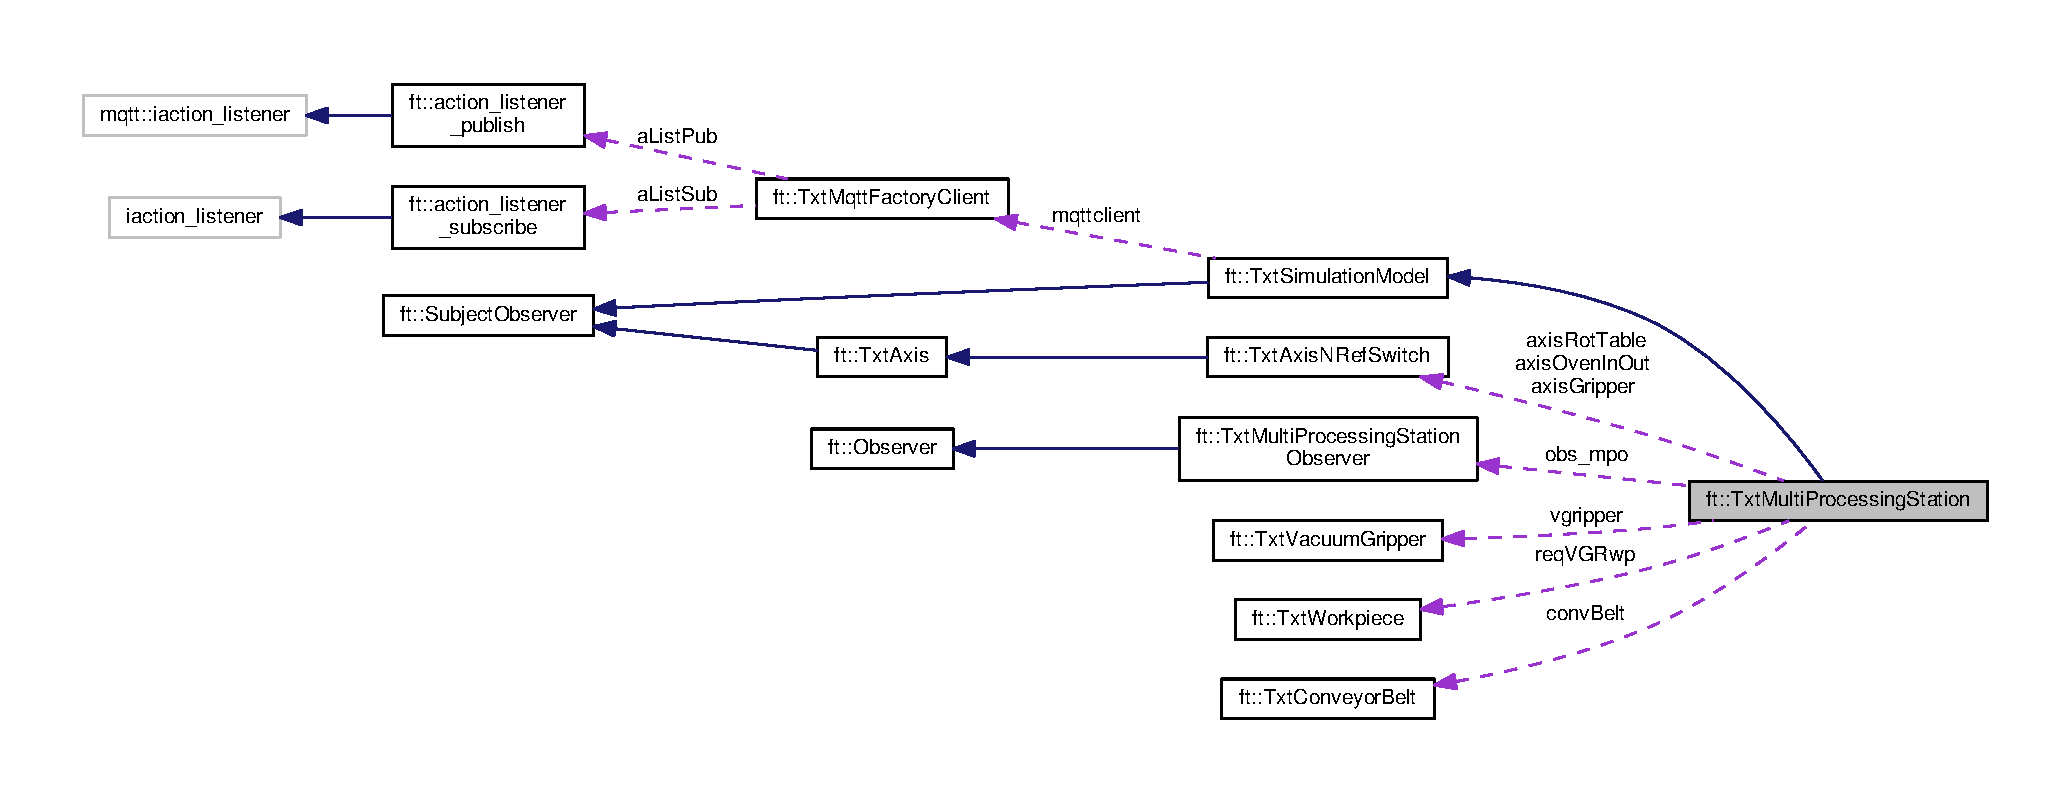
\includegraphics[width=350pt]{classft_1_1_txt_multi_processing_station__coll__graph}
\end{center}
\end{figure}
\subsection*{Public Types}
\begin{DoxyCompactItemize}
\item 
enum \hyperlink{classft_1_1_txt_multi_processing_station_a345fc850c7a3fd9062de2286a716fd2e}{State\+\_\+t} \{ \\*
\hyperlink{classft_1_1_txt_multi_processing_station_a345fc850c7a3fd9062de2286a716fd2eaa6f812e42b77ebbb1d01345241a97ee6}{\+\_\+\+\_\+\+N\+O\+\_\+\+S\+T\+A\+TE}, 
\hyperlink{classft_1_1_txt_multi_processing_station_a345fc850c7a3fd9062de2286a716fd2ea2ed60703ada004229c3ad40c9311e8dd}{F\+A\+U\+LT}, 
\hyperlink{classft_1_1_txt_multi_processing_station_a345fc850c7a3fd9062de2286a716fd2eaa581a2edb63e151be2262c22ec27a83e}{I\+N\+IT}, 
\hyperlink{classft_1_1_txt_multi_processing_station_a345fc850c7a3fd9062de2286a716fd2ea6040cee14c3dfc017178b474f10d51a8}{I\+D\+LE}, 
\\*
\hyperlink{classft_1_1_txt_multi_processing_station_a345fc850c7a3fd9062de2286a716fd2eac0575fae42d716e310d9daa2b32b3be4}{B\+U\+RN}, 
\hyperlink{classft_1_1_txt_multi_processing_station_a345fc850c7a3fd9062de2286a716fd2eaf596b7bbd3d7f3962ac2343cb3b9c7f6}{V\+G\+R\+\_\+\+T\+R\+A\+N\+S\+P\+O\+RT}, 
\hyperlink{classft_1_1_txt_multi_processing_station_a345fc850c7a3fd9062de2286a716fd2ea2693f8606855009a795f29ba2b085d7d}{T\+A\+B\+L\+E\+\_\+\+S\+AW}, 
\hyperlink{classft_1_1_txt_multi_processing_station_a345fc850c7a3fd9062de2286a716fd2ea5271ca81b86735673fa78ae47fc45984}{T\+A\+B\+L\+E\+\_\+\+B\+E\+LT}, 
\\*
\hyperlink{classft_1_1_txt_multi_processing_station_a345fc850c7a3fd9062de2286a716fd2ea56e16e258edac1722607561450104e1c}{E\+J\+E\+CT}, 
\hyperlink{classft_1_1_txt_multi_processing_station_a345fc850c7a3fd9062de2286a716fd2ea9d90004ee6699a8f1ce0987c6f1a4bc0}{T\+R\+A\+N\+S\+P\+O\+RT}
 \}
\end{DoxyCompactItemize}
\subsection*{Public Member Functions}
\begin{DoxyCompactItemize}
\item 
const char $\ast$ \hyperlink{classft_1_1_txt_multi_processing_station_a011660aedfc9db87528ea225dd1992d7}{to\+String} (\hyperlink{classft_1_1_txt_multi_processing_station_a345fc850c7a3fd9062de2286a716fd2e}{State\+\_\+t} state)
\item 
void \hyperlink{classft_1_1_txt_multi_processing_station_ac285715dcca171dc11881091b65d74ec}{print\+State} (\hyperlink{classft_1_1_txt_multi_processing_station_a345fc850c7a3fd9062de2286a716fd2e}{State\+\_\+t} state)
\item 
void \hyperlink{classft_1_1_txt_multi_processing_station_a2f4b727b06ad7ac5da1bec91944f9521}{print\+Entry\+State} (\hyperlink{classft_1_1_txt_multi_processing_station_a345fc850c7a3fd9062de2286a716fd2e}{State\+\_\+t} state)
\item 
void \hyperlink{classft_1_1_txt_multi_processing_station_acce7d500cc6c6c606e477a958a4b6fbe}{print\+Exit\+State} (\hyperlink{classft_1_1_txt_multi_processing_station_a345fc850c7a3fd9062de2286a716fd2e}{State\+\_\+t} state)
\item 
\hyperlink{classft_1_1_txt_multi_processing_station_aa24e16e04386fbc501a9db25d87c42e1}{Txt\+Multi\+Processing\+Station} (F\+I\+S\+H\+\_\+\+X1\+\_\+\+T\+R\+A\+N\+S\+F\+ER $\ast$\hyperlink{classft_1_1_txt_simulation_model_a9facd66a0dbecd676ae7b72c37a0b300}{p\+T\+Area}, \hyperlink{classft_1_1_txt_mqtt_factory_client}{ft\+::\+Txt\+Mqtt\+Factory\+Client} $\ast$\hyperlink{classft_1_1_txt_simulation_model_a6a92fdef8619b9b1636c7c464091ea3a}{mqttclient})
\item 
virtual \hyperlink{classft_1_1_txt_multi_processing_station_aa06cb8eca1b89da59412803dd90bc1b1}{$\sim$\+Txt\+Multi\+Processing\+Station} ()
\item 
void \hyperlink{classft_1_1_txt_multi_processing_station_a8f481b0f89f0968c2483a9eeae1fcb0b}{request\+Quit} ()
\item 
void \hyperlink{classft_1_1_txt_multi_processing_station_aba10b3958b9486516addc72da48412a5}{request\+V\+G\+Rproduce} (\hyperlink{classft_1_1_txt_workpiece}{Txt\+Workpiece} $\ast$wp)
\item 
void \hyperlink{classft_1_1_txt_multi_processing_station_aedf25609c07d4f50132567fdcddfd33d}{request\+S\+L\+Dstarted} ()
\item 
bool \hyperlink{classft_1_1_txt_multi_processing_station_a9abbcaf52138bafff050f52f574989e7}{is\+End\+Conveyor\+Belt\+Triggered} ()
\item 
void \hyperlink{classft_1_1_txt_multi_processing_station_a661ed9cee1b89aee262855bd03bbc371}{set\+Saw\+Off} ()
\item 
void \hyperlink{classft_1_1_txt_multi_processing_station_a0c4e7033897105daa634cf05ec1eb1d3}{set\+Saw\+Left} ()
\item 
void \hyperlink{classft_1_1_txt_multi_processing_station_af7e3e39a553c378d85f45fcf16ed2afe}{set\+Saw\+Right} ()
\item 
void \hyperlink{classft_1_1_txt_multi_processing_station_a302280bfcc3fc16a48a75746a249d603}{set\+Valve\+Ejection} (bool on)
\item 
void \hyperlink{classft_1_1_txt_multi_processing_station_a6cab40a75e0eccfe79fb0b1f65fb4ccb}{set\+Compressor} (bool on)
\item 
bool \hyperlink{classft_1_1_txt_multi_processing_station_ad49dbbf4007296e16f88e7d79a784e5c}{is\+Oven\+Triggered} ()
\item 
void \hyperlink{classft_1_1_txt_multi_processing_station_a2073f71234e6781c7eac48ff175f1c9a}{set\+Valve\+Vacuum} (bool on)
\item 
void \hyperlink{classft_1_1_txt_multi_processing_station_a9a6a259c42adea74fcc8b28bc252018f}{set\+Valve\+Lowering} (bool on)
\item 
void \hyperlink{classft_1_1_txt_multi_processing_station_abd0a00403958e599db70cfc7881ac36b}{set\+Valve\+Oven\+Door} (bool on)
\item 
void \hyperlink{classft_1_1_txt_multi_processing_station_a07d02c905529bf5adc7ad5bc5bbd7089}{set\+Light\+Oven} (bool on)
\end{DoxyCompactItemize}
\subsection*{Protected Member Functions}
\begin{DoxyCompactItemize}
\item 
void \hyperlink{classft_1_1_txt_multi_processing_station_a17489170af6848fd7545a514a16c6eb7}{config\+Inputs} ()
\item 
void \hyperlink{classft_1_1_txt_multi_processing_station_a5e660a44e3e5bbbcfd79bc73bc18a949}{run} ()
\end{DoxyCompactItemize}
\subsection*{Protected Attributes}
\begin{DoxyCompactItemize}
\item 
\hyperlink{classft_1_1_txt_multi_processing_station_a345fc850c7a3fd9062de2286a716fd2e}{State\+\_\+t} \hyperlink{classft_1_1_txt_multi_processing_station_aa6e7cf831e80c11a258aa778667384d0}{current\+State}
\item 
\hyperlink{classft_1_1_txt_multi_processing_station_a345fc850c7a3fd9062de2286a716fd2e}{State\+\_\+t} \hyperlink{classft_1_1_txt_multi_processing_station_af7f913b9865143d2b76fae771f9fa435}{new\+State}
\item 
uint8\+\_\+t \hyperlink{classft_1_1_txt_multi_processing_station_a1ca89d3f0f764e7576648484e5bd9d84}{ch\+Msaw}
\item 
\hyperlink{classft_1_1_txt_vacuum_gripper}{Txt\+Vacuum\+Gripper} \hyperlink{classft_1_1_txt_multi_processing_station_ae7185a6883fbf3ea0cd910495709476e}{vgripper}
\item 
\hyperlink{classft_1_1_txt_axis_n_ref_switch}{Txt\+Axis\+N\+Ref\+Switch} \hyperlink{classft_1_1_txt_multi_processing_station_a2340b3d052d5a07933e07b8752919fc9}{axis\+Gripper}
\item 
\hyperlink{classft_1_1_txt_axis_n_ref_switch}{Txt\+Axis\+N\+Ref\+Switch} \hyperlink{classft_1_1_txt_multi_processing_station_a357638bf052e8adf981d5cd297049a58}{axis\+Oven\+In\+Out}
\item 
\hyperlink{classft_1_1_txt_axis_n_ref_switch}{Txt\+Axis\+N\+Ref\+Switch} \hyperlink{classft_1_1_txt_multi_processing_station_a52704f5c21d82197cb2cff2845778ed2}{axis\+Rot\+Table}
\item 
\hyperlink{classft_1_1_txt_conveyor_belt}{Txt\+Conveyor\+Belt} \hyperlink{classft_1_1_txt_multi_processing_station_a4011960c442f32527a3880a77a2bf1c1}{conv\+Belt}
\item 
bool \hyperlink{classft_1_1_txt_multi_processing_station_addaf49d03f353087b40b96fb1173b959}{req\+Quit}
\item 
\hyperlink{classft_1_1_txt_workpiece}{Txt\+Workpiece} $\ast$ \hyperlink{classft_1_1_txt_multi_processing_station_a953cb7107d32b94809db4b0e8f2f9f2f}{req\+V\+G\+Rwp}
\item 
bool \hyperlink{classft_1_1_txt_multi_processing_station_afeac49b512ebfc99bf2632676d1e98c8}{req\+V\+G\+Rproduce}
\item 
bool \hyperlink{classft_1_1_txt_multi_processing_station_a3ad2570999a4e2087d29a1f4639527dc}{req\+S\+L\+Dstarted}
\item 
\hyperlink{classft_1_1_txt_multi_processing_station_observer}{Txt\+Multi\+Processing\+Station\+Observer} $\ast$ \hyperlink{classft_1_1_txt_multi_processing_station_a017a3f9bdbb577a12aaf9cc0ee301d8a}{obs\+\_\+mpo}
\end{DoxyCompactItemize}
\subsection*{Additional Inherited Members}


\subsection{Member Enumeration Documentation}
\index{ft\+::\+Txt\+Multi\+Processing\+Station@{ft\+::\+Txt\+Multi\+Processing\+Station}!State\+\_\+t@{State\+\_\+t}}
\index{State\+\_\+t@{State\+\_\+t}!ft\+::\+Txt\+Multi\+Processing\+Station@{ft\+::\+Txt\+Multi\+Processing\+Station}}
\subsubsection[{\texorpdfstring{State\+\_\+t}{State_t}}]{\setlength{\rightskip}{0pt plus 5cm}enum {\bf ft\+::\+Txt\+Multi\+Processing\+Station\+::\+State\+\_\+t}}\hypertarget{classft_1_1_txt_multi_processing_station_a345fc850c7a3fd9062de2286a716fd2e}{}\label{classft_1_1_txt_multi_processing_station_a345fc850c7a3fd9062de2286a716fd2e}
\begin{Desc}
\item[Enumerator]\par
\begin{description}
\index{\+\_\+\+\_\+\+N\+O\+\_\+\+S\+T\+A\+TE@{\+\_\+\+\_\+\+N\+O\+\_\+\+S\+T\+A\+TE}!ft\+::\+Txt\+Multi\+Processing\+Station@{ft\+::\+Txt\+Multi\+Processing\+Station}}\index{ft\+::\+Txt\+Multi\+Processing\+Station@{ft\+::\+Txt\+Multi\+Processing\+Station}!\+\_\+\+\_\+\+N\+O\+\_\+\+S\+T\+A\+TE@{\+\_\+\+\_\+\+N\+O\+\_\+\+S\+T\+A\+TE}}\item[{\em 
\+\_\+\+\_\+\+N\+O\+\_\+\+S\+T\+A\+TE\hypertarget{classft_1_1_txt_multi_processing_station_a345fc850c7a3fd9062de2286a716fd2eaa6f812e42b77ebbb1d01345241a97ee6}{}\label{classft_1_1_txt_multi_processing_station_a345fc850c7a3fd9062de2286a716fd2eaa6f812e42b77ebbb1d01345241a97ee6}
}]\index{F\+A\+U\+LT@{F\+A\+U\+LT}!ft\+::\+Txt\+Multi\+Processing\+Station@{ft\+::\+Txt\+Multi\+Processing\+Station}}\index{ft\+::\+Txt\+Multi\+Processing\+Station@{ft\+::\+Txt\+Multi\+Processing\+Station}!F\+A\+U\+LT@{F\+A\+U\+LT}}\item[{\em 
F\+A\+U\+LT\hypertarget{classft_1_1_txt_multi_processing_station_a345fc850c7a3fd9062de2286a716fd2ea2ed60703ada004229c3ad40c9311e8dd}{}\label{classft_1_1_txt_multi_processing_station_a345fc850c7a3fd9062de2286a716fd2ea2ed60703ada004229c3ad40c9311e8dd}
}]\index{I\+N\+IT@{I\+N\+IT}!ft\+::\+Txt\+Multi\+Processing\+Station@{ft\+::\+Txt\+Multi\+Processing\+Station}}\index{ft\+::\+Txt\+Multi\+Processing\+Station@{ft\+::\+Txt\+Multi\+Processing\+Station}!I\+N\+IT@{I\+N\+IT}}\item[{\em 
I\+N\+IT\hypertarget{classft_1_1_txt_multi_processing_station_a345fc850c7a3fd9062de2286a716fd2eaa581a2edb63e151be2262c22ec27a83e}{}\label{classft_1_1_txt_multi_processing_station_a345fc850c7a3fd9062de2286a716fd2eaa581a2edb63e151be2262c22ec27a83e}
}]\index{I\+D\+LE@{I\+D\+LE}!ft\+::\+Txt\+Multi\+Processing\+Station@{ft\+::\+Txt\+Multi\+Processing\+Station}}\index{ft\+::\+Txt\+Multi\+Processing\+Station@{ft\+::\+Txt\+Multi\+Processing\+Station}!I\+D\+LE@{I\+D\+LE}}\item[{\em 
I\+D\+LE\hypertarget{classft_1_1_txt_multi_processing_station_a345fc850c7a3fd9062de2286a716fd2ea6040cee14c3dfc017178b474f10d51a8}{}\label{classft_1_1_txt_multi_processing_station_a345fc850c7a3fd9062de2286a716fd2ea6040cee14c3dfc017178b474f10d51a8}
}]\index{B\+U\+RN@{B\+U\+RN}!ft\+::\+Txt\+Multi\+Processing\+Station@{ft\+::\+Txt\+Multi\+Processing\+Station}}\index{ft\+::\+Txt\+Multi\+Processing\+Station@{ft\+::\+Txt\+Multi\+Processing\+Station}!B\+U\+RN@{B\+U\+RN}}\item[{\em 
B\+U\+RN\hypertarget{classft_1_1_txt_multi_processing_station_a345fc850c7a3fd9062de2286a716fd2eac0575fae42d716e310d9daa2b32b3be4}{}\label{classft_1_1_txt_multi_processing_station_a345fc850c7a3fd9062de2286a716fd2eac0575fae42d716e310d9daa2b32b3be4}
}]\index{V\+G\+R\+\_\+\+T\+R\+A\+N\+S\+P\+O\+RT@{V\+G\+R\+\_\+\+T\+R\+A\+N\+S\+P\+O\+RT}!ft\+::\+Txt\+Multi\+Processing\+Station@{ft\+::\+Txt\+Multi\+Processing\+Station}}\index{ft\+::\+Txt\+Multi\+Processing\+Station@{ft\+::\+Txt\+Multi\+Processing\+Station}!V\+G\+R\+\_\+\+T\+R\+A\+N\+S\+P\+O\+RT@{V\+G\+R\+\_\+\+T\+R\+A\+N\+S\+P\+O\+RT}}\item[{\em 
V\+G\+R\+\_\+\+T\+R\+A\+N\+S\+P\+O\+RT\hypertarget{classft_1_1_txt_multi_processing_station_a345fc850c7a3fd9062de2286a716fd2eaf596b7bbd3d7f3962ac2343cb3b9c7f6}{}\label{classft_1_1_txt_multi_processing_station_a345fc850c7a3fd9062de2286a716fd2eaf596b7bbd3d7f3962ac2343cb3b9c7f6}
}]\index{T\+A\+B\+L\+E\+\_\+\+S\+AW@{T\+A\+B\+L\+E\+\_\+\+S\+AW}!ft\+::\+Txt\+Multi\+Processing\+Station@{ft\+::\+Txt\+Multi\+Processing\+Station}}\index{ft\+::\+Txt\+Multi\+Processing\+Station@{ft\+::\+Txt\+Multi\+Processing\+Station}!T\+A\+B\+L\+E\+\_\+\+S\+AW@{T\+A\+B\+L\+E\+\_\+\+S\+AW}}\item[{\em 
T\+A\+B\+L\+E\+\_\+\+S\+AW\hypertarget{classft_1_1_txt_multi_processing_station_a345fc850c7a3fd9062de2286a716fd2ea2693f8606855009a795f29ba2b085d7d}{}\label{classft_1_1_txt_multi_processing_station_a345fc850c7a3fd9062de2286a716fd2ea2693f8606855009a795f29ba2b085d7d}
}]\index{T\+A\+B\+L\+E\+\_\+\+B\+E\+LT@{T\+A\+B\+L\+E\+\_\+\+B\+E\+LT}!ft\+::\+Txt\+Multi\+Processing\+Station@{ft\+::\+Txt\+Multi\+Processing\+Station}}\index{ft\+::\+Txt\+Multi\+Processing\+Station@{ft\+::\+Txt\+Multi\+Processing\+Station}!T\+A\+B\+L\+E\+\_\+\+B\+E\+LT@{T\+A\+B\+L\+E\+\_\+\+B\+E\+LT}}\item[{\em 
T\+A\+B\+L\+E\+\_\+\+B\+E\+LT\hypertarget{classft_1_1_txt_multi_processing_station_a345fc850c7a3fd9062de2286a716fd2ea5271ca81b86735673fa78ae47fc45984}{}\label{classft_1_1_txt_multi_processing_station_a345fc850c7a3fd9062de2286a716fd2ea5271ca81b86735673fa78ae47fc45984}
}]\index{E\+J\+E\+CT@{E\+J\+E\+CT}!ft\+::\+Txt\+Multi\+Processing\+Station@{ft\+::\+Txt\+Multi\+Processing\+Station}}\index{ft\+::\+Txt\+Multi\+Processing\+Station@{ft\+::\+Txt\+Multi\+Processing\+Station}!E\+J\+E\+CT@{E\+J\+E\+CT}}\item[{\em 
E\+J\+E\+CT\hypertarget{classft_1_1_txt_multi_processing_station_a345fc850c7a3fd9062de2286a716fd2ea56e16e258edac1722607561450104e1c}{}\label{classft_1_1_txt_multi_processing_station_a345fc850c7a3fd9062de2286a716fd2ea56e16e258edac1722607561450104e1c}
}]\index{T\+R\+A\+N\+S\+P\+O\+RT@{T\+R\+A\+N\+S\+P\+O\+RT}!ft\+::\+Txt\+Multi\+Processing\+Station@{ft\+::\+Txt\+Multi\+Processing\+Station}}\index{ft\+::\+Txt\+Multi\+Processing\+Station@{ft\+::\+Txt\+Multi\+Processing\+Station}!T\+R\+A\+N\+S\+P\+O\+RT@{T\+R\+A\+N\+S\+P\+O\+RT}}\item[{\em 
T\+R\+A\+N\+S\+P\+O\+RT\hypertarget{classft_1_1_txt_multi_processing_station_a345fc850c7a3fd9062de2286a716fd2ea9d90004ee6699a8f1ce0987c6f1a4bc0}{}\label{classft_1_1_txt_multi_processing_station_a345fc850c7a3fd9062de2286a716fd2ea9d90004ee6699a8f1ce0987c6f1a4bc0}
}]\end{description}
\end{Desc}


\subsection{Constructor \& Destructor Documentation}
\index{ft\+::\+Txt\+Multi\+Processing\+Station@{ft\+::\+Txt\+Multi\+Processing\+Station}!Txt\+Multi\+Processing\+Station@{Txt\+Multi\+Processing\+Station}}
\index{Txt\+Multi\+Processing\+Station@{Txt\+Multi\+Processing\+Station}!ft\+::\+Txt\+Multi\+Processing\+Station@{ft\+::\+Txt\+Multi\+Processing\+Station}}
\subsubsection[{\texorpdfstring{Txt\+Multi\+Processing\+Station(\+F\+I\+S\+H\+\_\+\+X1\+\_\+\+T\+R\+A\+N\+S\+F\+E\+R $\ast$p\+T\+Area, ft\+::\+Txt\+Mqtt\+Factory\+Client $\ast$mqttclient)}{TxtMultiProcessingStation(FISH_X1_TRANSFER *pTArea, ft::TxtMqttFactoryClient *mqttclient)}}]{\setlength{\rightskip}{0pt plus 5cm}ft\+::\+Txt\+Multi\+Processing\+Station\+::\+Txt\+Multi\+Processing\+Station (
\begin{DoxyParamCaption}
\item[{F\+I\+S\+H\+\_\+\+X1\+\_\+\+T\+R\+A\+N\+S\+F\+ER $\ast$}]{p\+T\+Area, }
\item[{{\bf ft\+::\+Txt\+Mqtt\+Factory\+Client} $\ast$}]{mqttclient}
\end{DoxyParamCaption}
)}\hypertarget{classft_1_1_txt_multi_processing_station_aa24e16e04386fbc501a9db25d87c42e1}{}\label{classft_1_1_txt_multi_processing_station_aa24e16e04386fbc501a9db25d87c42e1}
\index{ft\+::\+Txt\+Multi\+Processing\+Station@{ft\+::\+Txt\+Multi\+Processing\+Station}!````~Txt\+Multi\+Processing\+Station@{$\sim$\+Txt\+Multi\+Processing\+Station}}
\index{````~Txt\+Multi\+Processing\+Station@{$\sim$\+Txt\+Multi\+Processing\+Station}!ft\+::\+Txt\+Multi\+Processing\+Station@{ft\+::\+Txt\+Multi\+Processing\+Station}}
\subsubsection[{\texorpdfstring{$\sim$\+Txt\+Multi\+Processing\+Station()}{~TxtMultiProcessingStation()}}]{\setlength{\rightskip}{0pt plus 5cm}virtual ft\+::\+Txt\+Multi\+Processing\+Station\+::$\sim$\+Txt\+Multi\+Processing\+Station (
\begin{DoxyParamCaption}
{}
\end{DoxyParamCaption}
)\hspace{0.3cm}{\ttfamily [virtual]}}\hypertarget{classft_1_1_txt_multi_processing_station_aa06cb8eca1b89da59412803dd90bc1b1}{}\label{classft_1_1_txt_multi_processing_station_aa06cb8eca1b89da59412803dd90bc1b1}


\subsection{Member Function Documentation}
\index{ft\+::\+Txt\+Multi\+Processing\+Station@{ft\+::\+Txt\+Multi\+Processing\+Station}!config\+Inputs@{config\+Inputs}}
\index{config\+Inputs@{config\+Inputs}!ft\+::\+Txt\+Multi\+Processing\+Station@{ft\+::\+Txt\+Multi\+Processing\+Station}}
\subsubsection[{\texorpdfstring{config\+Inputs()}{configInputs()}}]{\setlength{\rightskip}{0pt plus 5cm}void ft\+::\+Txt\+Multi\+Processing\+Station\+::config\+Inputs (
\begin{DoxyParamCaption}
{}
\end{DoxyParamCaption}
)\hspace{0.3cm}{\ttfamily [protected]}}\hypertarget{classft_1_1_txt_multi_processing_station_a17489170af6848fd7545a514a16c6eb7}{}\label{classft_1_1_txt_multi_processing_station_a17489170af6848fd7545a514a16c6eb7}
\index{ft\+::\+Txt\+Multi\+Processing\+Station@{ft\+::\+Txt\+Multi\+Processing\+Station}!is\+End\+Conveyor\+Belt\+Triggered@{is\+End\+Conveyor\+Belt\+Triggered}}
\index{is\+End\+Conveyor\+Belt\+Triggered@{is\+End\+Conveyor\+Belt\+Triggered}!ft\+::\+Txt\+Multi\+Processing\+Station@{ft\+::\+Txt\+Multi\+Processing\+Station}}
\subsubsection[{\texorpdfstring{is\+End\+Conveyor\+Belt\+Triggered()}{isEndConveyorBeltTriggered()}}]{\setlength{\rightskip}{0pt plus 5cm}bool ft\+::\+Txt\+Multi\+Processing\+Station\+::is\+End\+Conveyor\+Belt\+Triggered (
\begin{DoxyParamCaption}
{}
\end{DoxyParamCaption}
)}\hypertarget{classft_1_1_txt_multi_processing_station_a9abbcaf52138bafff050f52f574989e7}{}\label{classft_1_1_txt_multi_processing_station_a9abbcaf52138bafff050f52f574989e7}
\index{ft\+::\+Txt\+Multi\+Processing\+Station@{ft\+::\+Txt\+Multi\+Processing\+Station}!is\+Oven\+Triggered@{is\+Oven\+Triggered}}
\index{is\+Oven\+Triggered@{is\+Oven\+Triggered}!ft\+::\+Txt\+Multi\+Processing\+Station@{ft\+::\+Txt\+Multi\+Processing\+Station}}
\subsubsection[{\texorpdfstring{is\+Oven\+Triggered()}{isOvenTriggered()}}]{\setlength{\rightskip}{0pt plus 5cm}bool ft\+::\+Txt\+Multi\+Processing\+Station\+::is\+Oven\+Triggered (
\begin{DoxyParamCaption}
{}
\end{DoxyParamCaption}
)}\hypertarget{classft_1_1_txt_multi_processing_station_ad49dbbf4007296e16f88e7d79a784e5c}{}\label{classft_1_1_txt_multi_processing_station_ad49dbbf4007296e16f88e7d79a784e5c}
\index{ft\+::\+Txt\+Multi\+Processing\+Station@{ft\+::\+Txt\+Multi\+Processing\+Station}!print\+Entry\+State@{print\+Entry\+State}}
\index{print\+Entry\+State@{print\+Entry\+State}!ft\+::\+Txt\+Multi\+Processing\+Station@{ft\+::\+Txt\+Multi\+Processing\+Station}}
\subsubsection[{\texorpdfstring{print\+Entry\+State(\+State\+\_\+t state)}{printEntryState(State_t state)}}]{\setlength{\rightskip}{0pt plus 5cm}void ft\+::\+Txt\+Multi\+Processing\+Station\+::print\+Entry\+State (
\begin{DoxyParamCaption}
\item[{{\bf State\+\_\+t}}]{state}
\end{DoxyParamCaption}
)\hspace{0.3cm}{\ttfamily [inline]}}\hypertarget{classft_1_1_txt_multi_processing_station_a2f4b727b06ad7ac5da1bec91944f9521}{}\label{classft_1_1_txt_multi_processing_station_a2f4b727b06ad7ac5da1bec91944f9521}
\index{ft\+::\+Txt\+Multi\+Processing\+Station@{ft\+::\+Txt\+Multi\+Processing\+Station}!print\+Exit\+State@{print\+Exit\+State}}
\index{print\+Exit\+State@{print\+Exit\+State}!ft\+::\+Txt\+Multi\+Processing\+Station@{ft\+::\+Txt\+Multi\+Processing\+Station}}
\subsubsection[{\texorpdfstring{print\+Exit\+State(\+State\+\_\+t state)}{printExitState(State_t state)}}]{\setlength{\rightskip}{0pt plus 5cm}void ft\+::\+Txt\+Multi\+Processing\+Station\+::print\+Exit\+State (
\begin{DoxyParamCaption}
\item[{{\bf State\+\_\+t}}]{state}
\end{DoxyParamCaption}
)\hspace{0.3cm}{\ttfamily [inline]}}\hypertarget{classft_1_1_txt_multi_processing_station_acce7d500cc6c6c606e477a958a4b6fbe}{}\label{classft_1_1_txt_multi_processing_station_acce7d500cc6c6c606e477a958a4b6fbe}
\index{ft\+::\+Txt\+Multi\+Processing\+Station@{ft\+::\+Txt\+Multi\+Processing\+Station}!print\+State@{print\+State}}
\index{print\+State@{print\+State}!ft\+::\+Txt\+Multi\+Processing\+Station@{ft\+::\+Txt\+Multi\+Processing\+Station}}
\subsubsection[{\texorpdfstring{print\+State(\+State\+\_\+t state)}{printState(State_t state)}}]{\setlength{\rightskip}{0pt plus 5cm}void ft\+::\+Txt\+Multi\+Processing\+Station\+::print\+State (
\begin{DoxyParamCaption}
\item[{{\bf State\+\_\+t}}]{state}
\end{DoxyParamCaption}
)\hspace{0.3cm}{\ttfamily [inline]}}\hypertarget{classft_1_1_txt_multi_processing_station_ac285715dcca171dc11881091b65d74ec}{}\label{classft_1_1_txt_multi_processing_station_ac285715dcca171dc11881091b65d74ec}
\index{ft\+::\+Txt\+Multi\+Processing\+Station@{ft\+::\+Txt\+Multi\+Processing\+Station}!request\+Quit@{request\+Quit}}
\index{request\+Quit@{request\+Quit}!ft\+::\+Txt\+Multi\+Processing\+Station@{ft\+::\+Txt\+Multi\+Processing\+Station}}
\subsubsection[{\texorpdfstring{request\+Quit()}{requestQuit()}}]{\setlength{\rightskip}{0pt plus 5cm}void ft\+::\+Txt\+Multi\+Processing\+Station\+::request\+Quit (
\begin{DoxyParamCaption}
{}
\end{DoxyParamCaption}
)\hspace{0.3cm}{\ttfamily [inline]}}\hypertarget{classft_1_1_txt_multi_processing_station_a8f481b0f89f0968c2483a9eeae1fcb0b}{}\label{classft_1_1_txt_multi_processing_station_a8f481b0f89f0968c2483a9eeae1fcb0b}
\index{ft\+::\+Txt\+Multi\+Processing\+Station@{ft\+::\+Txt\+Multi\+Processing\+Station}!request\+S\+L\+Dstarted@{request\+S\+L\+Dstarted}}
\index{request\+S\+L\+Dstarted@{request\+S\+L\+Dstarted}!ft\+::\+Txt\+Multi\+Processing\+Station@{ft\+::\+Txt\+Multi\+Processing\+Station}}
\subsubsection[{\texorpdfstring{request\+S\+L\+Dstarted()}{requestSLDstarted()}}]{\setlength{\rightskip}{0pt plus 5cm}void ft\+::\+Txt\+Multi\+Processing\+Station\+::request\+S\+L\+Dstarted (
\begin{DoxyParamCaption}
{}
\end{DoxyParamCaption}
)\hspace{0.3cm}{\ttfamily [inline]}}\hypertarget{classft_1_1_txt_multi_processing_station_aedf25609c07d4f50132567fdcddfd33d}{}\label{classft_1_1_txt_multi_processing_station_aedf25609c07d4f50132567fdcddfd33d}
\index{ft\+::\+Txt\+Multi\+Processing\+Station@{ft\+::\+Txt\+Multi\+Processing\+Station}!request\+V\+G\+Rproduce@{request\+V\+G\+Rproduce}}
\index{request\+V\+G\+Rproduce@{request\+V\+G\+Rproduce}!ft\+::\+Txt\+Multi\+Processing\+Station@{ft\+::\+Txt\+Multi\+Processing\+Station}}
\subsubsection[{\texorpdfstring{request\+V\+G\+Rproduce(\+Txt\+Workpiece $\ast$wp)}{requestVGRproduce(TxtWorkpiece *wp)}}]{\setlength{\rightskip}{0pt plus 5cm}void ft\+::\+Txt\+Multi\+Processing\+Station\+::request\+V\+G\+Rproduce (
\begin{DoxyParamCaption}
\item[{{\bf Txt\+Workpiece} $\ast$}]{wp}
\end{DoxyParamCaption}
)\hspace{0.3cm}{\ttfamily [inline]}}\hypertarget{classft_1_1_txt_multi_processing_station_aba10b3958b9486516addc72da48412a5}{}\label{classft_1_1_txt_multi_processing_station_aba10b3958b9486516addc72da48412a5}
\index{ft\+::\+Txt\+Multi\+Processing\+Station@{ft\+::\+Txt\+Multi\+Processing\+Station}!run@{run}}
\index{run@{run}!ft\+::\+Txt\+Multi\+Processing\+Station@{ft\+::\+Txt\+Multi\+Processing\+Station}}
\subsubsection[{\texorpdfstring{run()}{run()}}]{\setlength{\rightskip}{0pt plus 5cm}void ft\+::\+Txt\+Multi\+Processing\+Station\+::run (
\begin{DoxyParamCaption}
{}
\end{DoxyParamCaption}
)\hspace{0.3cm}{\ttfamily [protected]}, {\ttfamily [virtual]}}\hypertarget{classft_1_1_txt_multi_processing_station_a5e660a44e3e5bbbcfd79bc73bc18a949}{}\label{classft_1_1_txt_multi_processing_station_a5e660a44e3e5bbbcfd79bc73bc18a949}

\begin{DoxyImageNoCaption}
  \mbox{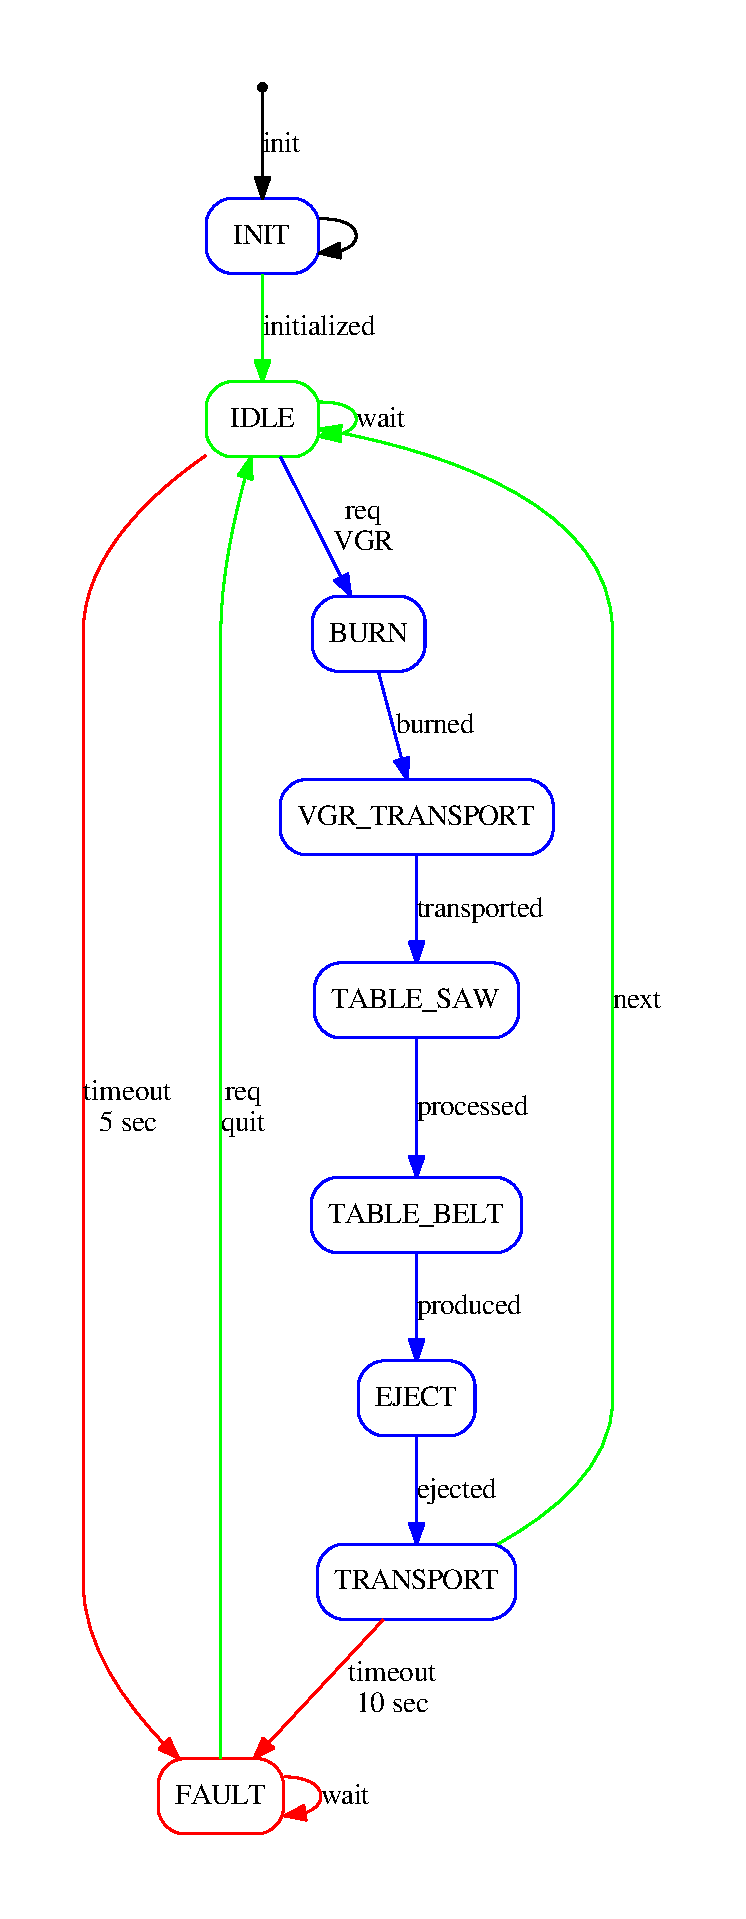
\includegraphics[width=\textwidth,height=\textheight/2,keepaspectratio=true]{dot_TxtMultiProcessingStationRun}}
\end{DoxyImageNoCaption}
 

Implements \hyperlink{classft_1_1_txt_simulation_model_a91595c8fc91104e98d2ea13fe349b777}{ft\+::\+Txt\+Simulation\+Model}.

\index{ft\+::\+Txt\+Multi\+Processing\+Station@{ft\+::\+Txt\+Multi\+Processing\+Station}!set\+Compressor@{set\+Compressor}}
\index{set\+Compressor@{set\+Compressor}!ft\+::\+Txt\+Multi\+Processing\+Station@{ft\+::\+Txt\+Multi\+Processing\+Station}}
\subsubsection[{\texorpdfstring{set\+Compressor(bool on)}{setCompressor(bool on)}}]{\setlength{\rightskip}{0pt plus 5cm}void ft\+::\+Txt\+Multi\+Processing\+Station\+::set\+Compressor (
\begin{DoxyParamCaption}
\item[{bool}]{on}
\end{DoxyParamCaption}
)}\hypertarget{classft_1_1_txt_multi_processing_station_a6cab40a75e0eccfe79fb0b1f65fb4ccb}{}\label{classft_1_1_txt_multi_processing_station_a6cab40a75e0eccfe79fb0b1f65fb4ccb}
\index{ft\+::\+Txt\+Multi\+Processing\+Station@{ft\+::\+Txt\+Multi\+Processing\+Station}!set\+Light\+Oven@{set\+Light\+Oven}}
\index{set\+Light\+Oven@{set\+Light\+Oven}!ft\+::\+Txt\+Multi\+Processing\+Station@{ft\+::\+Txt\+Multi\+Processing\+Station}}
\subsubsection[{\texorpdfstring{set\+Light\+Oven(bool on)}{setLightOven(bool on)}}]{\setlength{\rightskip}{0pt plus 5cm}void ft\+::\+Txt\+Multi\+Processing\+Station\+::set\+Light\+Oven (
\begin{DoxyParamCaption}
\item[{bool}]{on}
\end{DoxyParamCaption}
)}\hypertarget{classft_1_1_txt_multi_processing_station_a07d02c905529bf5adc7ad5bc5bbd7089}{}\label{classft_1_1_txt_multi_processing_station_a07d02c905529bf5adc7ad5bc5bbd7089}
\index{ft\+::\+Txt\+Multi\+Processing\+Station@{ft\+::\+Txt\+Multi\+Processing\+Station}!set\+Saw\+Left@{set\+Saw\+Left}}
\index{set\+Saw\+Left@{set\+Saw\+Left}!ft\+::\+Txt\+Multi\+Processing\+Station@{ft\+::\+Txt\+Multi\+Processing\+Station}}
\subsubsection[{\texorpdfstring{set\+Saw\+Left()}{setSawLeft()}}]{\setlength{\rightskip}{0pt plus 5cm}void ft\+::\+Txt\+Multi\+Processing\+Station\+::set\+Saw\+Left (
\begin{DoxyParamCaption}
{}
\end{DoxyParamCaption}
)}\hypertarget{classft_1_1_txt_multi_processing_station_a0c4e7033897105daa634cf05ec1eb1d3}{}\label{classft_1_1_txt_multi_processing_station_a0c4e7033897105daa634cf05ec1eb1d3}
\index{ft\+::\+Txt\+Multi\+Processing\+Station@{ft\+::\+Txt\+Multi\+Processing\+Station}!set\+Saw\+Off@{set\+Saw\+Off}}
\index{set\+Saw\+Off@{set\+Saw\+Off}!ft\+::\+Txt\+Multi\+Processing\+Station@{ft\+::\+Txt\+Multi\+Processing\+Station}}
\subsubsection[{\texorpdfstring{set\+Saw\+Off()}{setSawOff()}}]{\setlength{\rightskip}{0pt plus 5cm}void ft\+::\+Txt\+Multi\+Processing\+Station\+::set\+Saw\+Off (
\begin{DoxyParamCaption}
{}
\end{DoxyParamCaption}
)}\hypertarget{classft_1_1_txt_multi_processing_station_a661ed9cee1b89aee262855bd03bbc371}{}\label{classft_1_1_txt_multi_processing_station_a661ed9cee1b89aee262855bd03bbc371}
\index{ft\+::\+Txt\+Multi\+Processing\+Station@{ft\+::\+Txt\+Multi\+Processing\+Station}!set\+Saw\+Right@{set\+Saw\+Right}}
\index{set\+Saw\+Right@{set\+Saw\+Right}!ft\+::\+Txt\+Multi\+Processing\+Station@{ft\+::\+Txt\+Multi\+Processing\+Station}}
\subsubsection[{\texorpdfstring{set\+Saw\+Right()}{setSawRight()}}]{\setlength{\rightskip}{0pt plus 5cm}void ft\+::\+Txt\+Multi\+Processing\+Station\+::set\+Saw\+Right (
\begin{DoxyParamCaption}
{}
\end{DoxyParamCaption}
)}\hypertarget{classft_1_1_txt_multi_processing_station_af7e3e39a553c378d85f45fcf16ed2afe}{}\label{classft_1_1_txt_multi_processing_station_af7e3e39a553c378d85f45fcf16ed2afe}
\index{ft\+::\+Txt\+Multi\+Processing\+Station@{ft\+::\+Txt\+Multi\+Processing\+Station}!set\+Valve\+Ejection@{set\+Valve\+Ejection}}
\index{set\+Valve\+Ejection@{set\+Valve\+Ejection}!ft\+::\+Txt\+Multi\+Processing\+Station@{ft\+::\+Txt\+Multi\+Processing\+Station}}
\subsubsection[{\texorpdfstring{set\+Valve\+Ejection(bool on)}{setValveEjection(bool on)}}]{\setlength{\rightskip}{0pt plus 5cm}void ft\+::\+Txt\+Multi\+Processing\+Station\+::set\+Valve\+Ejection (
\begin{DoxyParamCaption}
\item[{bool}]{on}
\end{DoxyParamCaption}
)}\hypertarget{classft_1_1_txt_multi_processing_station_a302280bfcc3fc16a48a75746a249d603}{}\label{classft_1_1_txt_multi_processing_station_a302280bfcc3fc16a48a75746a249d603}
\index{ft\+::\+Txt\+Multi\+Processing\+Station@{ft\+::\+Txt\+Multi\+Processing\+Station}!set\+Valve\+Lowering@{set\+Valve\+Lowering}}
\index{set\+Valve\+Lowering@{set\+Valve\+Lowering}!ft\+::\+Txt\+Multi\+Processing\+Station@{ft\+::\+Txt\+Multi\+Processing\+Station}}
\subsubsection[{\texorpdfstring{set\+Valve\+Lowering(bool on)}{setValveLowering(bool on)}}]{\setlength{\rightskip}{0pt plus 5cm}void ft\+::\+Txt\+Multi\+Processing\+Station\+::set\+Valve\+Lowering (
\begin{DoxyParamCaption}
\item[{bool}]{on}
\end{DoxyParamCaption}
)}\hypertarget{classft_1_1_txt_multi_processing_station_a9a6a259c42adea74fcc8b28bc252018f}{}\label{classft_1_1_txt_multi_processing_station_a9a6a259c42adea74fcc8b28bc252018f}
\index{ft\+::\+Txt\+Multi\+Processing\+Station@{ft\+::\+Txt\+Multi\+Processing\+Station}!set\+Valve\+Oven\+Door@{set\+Valve\+Oven\+Door}}
\index{set\+Valve\+Oven\+Door@{set\+Valve\+Oven\+Door}!ft\+::\+Txt\+Multi\+Processing\+Station@{ft\+::\+Txt\+Multi\+Processing\+Station}}
\subsubsection[{\texorpdfstring{set\+Valve\+Oven\+Door(bool on)}{setValveOvenDoor(bool on)}}]{\setlength{\rightskip}{0pt plus 5cm}void ft\+::\+Txt\+Multi\+Processing\+Station\+::set\+Valve\+Oven\+Door (
\begin{DoxyParamCaption}
\item[{bool}]{on}
\end{DoxyParamCaption}
)}\hypertarget{classft_1_1_txt_multi_processing_station_abd0a00403958e599db70cfc7881ac36b}{}\label{classft_1_1_txt_multi_processing_station_abd0a00403958e599db70cfc7881ac36b}
\index{ft\+::\+Txt\+Multi\+Processing\+Station@{ft\+::\+Txt\+Multi\+Processing\+Station}!set\+Valve\+Vacuum@{set\+Valve\+Vacuum}}
\index{set\+Valve\+Vacuum@{set\+Valve\+Vacuum}!ft\+::\+Txt\+Multi\+Processing\+Station@{ft\+::\+Txt\+Multi\+Processing\+Station}}
\subsubsection[{\texorpdfstring{set\+Valve\+Vacuum(bool on)}{setValveVacuum(bool on)}}]{\setlength{\rightskip}{0pt plus 5cm}void ft\+::\+Txt\+Multi\+Processing\+Station\+::set\+Valve\+Vacuum (
\begin{DoxyParamCaption}
\item[{bool}]{on}
\end{DoxyParamCaption}
)}\hypertarget{classft_1_1_txt_multi_processing_station_a2073f71234e6781c7eac48ff175f1c9a}{}\label{classft_1_1_txt_multi_processing_station_a2073f71234e6781c7eac48ff175f1c9a}
\index{ft\+::\+Txt\+Multi\+Processing\+Station@{ft\+::\+Txt\+Multi\+Processing\+Station}!to\+String@{to\+String}}
\index{to\+String@{to\+String}!ft\+::\+Txt\+Multi\+Processing\+Station@{ft\+::\+Txt\+Multi\+Processing\+Station}}
\subsubsection[{\texorpdfstring{to\+String(\+State\+\_\+t state)}{toString(State_t state)}}]{\setlength{\rightskip}{0pt plus 5cm}const char$\ast$ ft\+::\+Txt\+Multi\+Processing\+Station\+::to\+String (
\begin{DoxyParamCaption}
\item[{{\bf State\+\_\+t}}]{state}
\end{DoxyParamCaption}
)\hspace{0.3cm}{\ttfamily [inline]}}\hypertarget{classft_1_1_txt_multi_processing_station_a011660aedfc9db87528ea225dd1992d7}{}\label{classft_1_1_txt_multi_processing_station_a011660aedfc9db87528ea225dd1992d7}


\subsection{Member Data Documentation}
\index{ft\+::\+Txt\+Multi\+Processing\+Station@{ft\+::\+Txt\+Multi\+Processing\+Station}!axis\+Gripper@{axis\+Gripper}}
\index{axis\+Gripper@{axis\+Gripper}!ft\+::\+Txt\+Multi\+Processing\+Station@{ft\+::\+Txt\+Multi\+Processing\+Station}}
\subsubsection[{\texorpdfstring{axis\+Gripper}{axisGripper}}]{\setlength{\rightskip}{0pt plus 5cm}{\bf Txt\+Axis\+N\+Ref\+Switch} ft\+::\+Txt\+Multi\+Processing\+Station\+::axis\+Gripper\hspace{0.3cm}{\ttfamily [protected]}}\hypertarget{classft_1_1_txt_multi_processing_station_a2340b3d052d5a07933e07b8752919fc9}{}\label{classft_1_1_txt_multi_processing_station_a2340b3d052d5a07933e07b8752919fc9}
\index{ft\+::\+Txt\+Multi\+Processing\+Station@{ft\+::\+Txt\+Multi\+Processing\+Station}!axis\+Oven\+In\+Out@{axis\+Oven\+In\+Out}}
\index{axis\+Oven\+In\+Out@{axis\+Oven\+In\+Out}!ft\+::\+Txt\+Multi\+Processing\+Station@{ft\+::\+Txt\+Multi\+Processing\+Station}}
\subsubsection[{\texorpdfstring{axis\+Oven\+In\+Out}{axisOvenInOut}}]{\setlength{\rightskip}{0pt plus 5cm}{\bf Txt\+Axis\+N\+Ref\+Switch} ft\+::\+Txt\+Multi\+Processing\+Station\+::axis\+Oven\+In\+Out\hspace{0.3cm}{\ttfamily [protected]}}\hypertarget{classft_1_1_txt_multi_processing_station_a357638bf052e8adf981d5cd297049a58}{}\label{classft_1_1_txt_multi_processing_station_a357638bf052e8adf981d5cd297049a58}
\index{ft\+::\+Txt\+Multi\+Processing\+Station@{ft\+::\+Txt\+Multi\+Processing\+Station}!axis\+Rot\+Table@{axis\+Rot\+Table}}
\index{axis\+Rot\+Table@{axis\+Rot\+Table}!ft\+::\+Txt\+Multi\+Processing\+Station@{ft\+::\+Txt\+Multi\+Processing\+Station}}
\subsubsection[{\texorpdfstring{axis\+Rot\+Table}{axisRotTable}}]{\setlength{\rightskip}{0pt plus 5cm}{\bf Txt\+Axis\+N\+Ref\+Switch} ft\+::\+Txt\+Multi\+Processing\+Station\+::axis\+Rot\+Table\hspace{0.3cm}{\ttfamily [protected]}}\hypertarget{classft_1_1_txt_multi_processing_station_a52704f5c21d82197cb2cff2845778ed2}{}\label{classft_1_1_txt_multi_processing_station_a52704f5c21d82197cb2cff2845778ed2}
\index{ft\+::\+Txt\+Multi\+Processing\+Station@{ft\+::\+Txt\+Multi\+Processing\+Station}!ch\+Msaw@{ch\+Msaw}}
\index{ch\+Msaw@{ch\+Msaw}!ft\+::\+Txt\+Multi\+Processing\+Station@{ft\+::\+Txt\+Multi\+Processing\+Station}}
\subsubsection[{\texorpdfstring{ch\+Msaw}{chMsaw}}]{\setlength{\rightskip}{0pt plus 5cm}uint8\+\_\+t ft\+::\+Txt\+Multi\+Processing\+Station\+::ch\+Msaw\hspace{0.3cm}{\ttfamily [protected]}}\hypertarget{classft_1_1_txt_multi_processing_station_a1ca89d3f0f764e7576648484e5bd9d84}{}\label{classft_1_1_txt_multi_processing_station_a1ca89d3f0f764e7576648484e5bd9d84}
\index{ft\+::\+Txt\+Multi\+Processing\+Station@{ft\+::\+Txt\+Multi\+Processing\+Station}!conv\+Belt@{conv\+Belt}}
\index{conv\+Belt@{conv\+Belt}!ft\+::\+Txt\+Multi\+Processing\+Station@{ft\+::\+Txt\+Multi\+Processing\+Station}}
\subsubsection[{\texorpdfstring{conv\+Belt}{convBelt}}]{\setlength{\rightskip}{0pt plus 5cm}{\bf Txt\+Conveyor\+Belt} ft\+::\+Txt\+Multi\+Processing\+Station\+::conv\+Belt\hspace{0.3cm}{\ttfamily [protected]}}\hypertarget{classft_1_1_txt_multi_processing_station_a4011960c442f32527a3880a77a2bf1c1}{}\label{classft_1_1_txt_multi_processing_station_a4011960c442f32527a3880a77a2bf1c1}
\index{ft\+::\+Txt\+Multi\+Processing\+Station@{ft\+::\+Txt\+Multi\+Processing\+Station}!current\+State@{current\+State}}
\index{current\+State@{current\+State}!ft\+::\+Txt\+Multi\+Processing\+Station@{ft\+::\+Txt\+Multi\+Processing\+Station}}
\subsubsection[{\texorpdfstring{current\+State}{currentState}}]{\setlength{\rightskip}{0pt plus 5cm}{\bf State\+\_\+t} ft\+::\+Txt\+Multi\+Processing\+Station\+::current\+State\hspace{0.3cm}{\ttfamily [protected]}}\hypertarget{classft_1_1_txt_multi_processing_station_aa6e7cf831e80c11a258aa778667384d0}{}\label{classft_1_1_txt_multi_processing_station_aa6e7cf831e80c11a258aa778667384d0}
\index{ft\+::\+Txt\+Multi\+Processing\+Station@{ft\+::\+Txt\+Multi\+Processing\+Station}!new\+State@{new\+State}}
\index{new\+State@{new\+State}!ft\+::\+Txt\+Multi\+Processing\+Station@{ft\+::\+Txt\+Multi\+Processing\+Station}}
\subsubsection[{\texorpdfstring{new\+State}{newState}}]{\setlength{\rightskip}{0pt plus 5cm}{\bf State\+\_\+t} ft\+::\+Txt\+Multi\+Processing\+Station\+::new\+State\hspace{0.3cm}{\ttfamily [protected]}}\hypertarget{classft_1_1_txt_multi_processing_station_af7f913b9865143d2b76fae771f9fa435}{}\label{classft_1_1_txt_multi_processing_station_af7f913b9865143d2b76fae771f9fa435}
\index{ft\+::\+Txt\+Multi\+Processing\+Station@{ft\+::\+Txt\+Multi\+Processing\+Station}!obs\+\_\+mpo@{obs\+\_\+mpo}}
\index{obs\+\_\+mpo@{obs\+\_\+mpo}!ft\+::\+Txt\+Multi\+Processing\+Station@{ft\+::\+Txt\+Multi\+Processing\+Station}}
\subsubsection[{\texorpdfstring{obs\+\_\+mpo}{obs_mpo}}]{\setlength{\rightskip}{0pt plus 5cm}{\bf Txt\+Multi\+Processing\+Station\+Observer}$\ast$ ft\+::\+Txt\+Multi\+Processing\+Station\+::obs\+\_\+mpo\hspace{0.3cm}{\ttfamily [protected]}}\hypertarget{classft_1_1_txt_multi_processing_station_a017a3f9bdbb577a12aaf9cc0ee301d8a}{}\label{classft_1_1_txt_multi_processing_station_a017a3f9bdbb577a12aaf9cc0ee301d8a}
\index{ft\+::\+Txt\+Multi\+Processing\+Station@{ft\+::\+Txt\+Multi\+Processing\+Station}!req\+Quit@{req\+Quit}}
\index{req\+Quit@{req\+Quit}!ft\+::\+Txt\+Multi\+Processing\+Station@{ft\+::\+Txt\+Multi\+Processing\+Station}}
\subsubsection[{\texorpdfstring{req\+Quit}{reqQuit}}]{\setlength{\rightskip}{0pt plus 5cm}bool ft\+::\+Txt\+Multi\+Processing\+Station\+::req\+Quit\hspace{0.3cm}{\ttfamily [protected]}}\hypertarget{classft_1_1_txt_multi_processing_station_addaf49d03f353087b40b96fb1173b959}{}\label{classft_1_1_txt_multi_processing_station_addaf49d03f353087b40b96fb1173b959}
\index{ft\+::\+Txt\+Multi\+Processing\+Station@{ft\+::\+Txt\+Multi\+Processing\+Station}!req\+S\+L\+Dstarted@{req\+S\+L\+Dstarted}}
\index{req\+S\+L\+Dstarted@{req\+S\+L\+Dstarted}!ft\+::\+Txt\+Multi\+Processing\+Station@{ft\+::\+Txt\+Multi\+Processing\+Station}}
\subsubsection[{\texorpdfstring{req\+S\+L\+Dstarted}{reqSLDstarted}}]{\setlength{\rightskip}{0pt plus 5cm}bool ft\+::\+Txt\+Multi\+Processing\+Station\+::req\+S\+L\+Dstarted\hspace{0.3cm}{\ttfamily [protected]}}\hypertarget{classft_1_1_txt_multi_processing_station_a3ad2570999a4e2087d29a1f4639527dc}{}\label{classft_1_1_txt_multi_processing_station_a3ad2570999a4e2087d29a1f4639527dc}
\index{ft\+::\+Txt\+Multi\+Processing\+Station@{ft\+::\+Txt\+Multi\+Processing\+Station}!req\+V\+G\+Rproduce@{req\+V\+G\+Rproduce}}
\index{req\+V\+G\+Rproduce@{req\+V\+G\+Rproduce}!ft\+::\+Txt\+Multi\+Processing\+Station@{ft\+::\+Txt\+Multi\+Processing\+Station}}
\subsubsection[{\texorpdfstring{req\+V\+G\+Rproduce}{reqVGRproduce}}]{\setlength{\rightskip}{0pt plus 5cm}bool ft\+::\+Txt\+Multi\+Processing\+Station\+::req\+V\+G\+Rproduce\hspace{0.3cm}{\ttfamily [protected]}}\hypertarget{classft_1_1_txt_multi_processing_station_afeac49b512ebfc99bf2632676d1e98c8}{}\label{classft_1_1_txt_multi_processing_station_afeac49b512ebfc99bf2632676d1e98c8}
\index{ft\+::\+Txt\+Multi\+Processing\+Station@{ft\+::\+Txt\+Multi\+Processing\+Station}!req\+V\+G\+Rwp@{req\+V\+G\+Rwp}}
\index{req\+V\+G\+Rwp@{req\+V\+G\+Rwp}!ft\+::\+Txt\+Multi\+Processing\+Station@{ft\+::\+Txt\+Multi\+Processing\+Station}}
\subsubsection[{\texorpdfstring{req\+V\+G\+Rwp}{reqVGRwp}}]{\setlength{\rightskip}{0pt plus 5cm}{\bf Txt\+Workpiece}$\ast$ ft\+::\+Txt\+Multi\+Processing\+Station\+::req\+V\+G\+Rwp\hspace{0.3cm}{\ttfamily [protected]}}\hypertarget{classft_1_1_txt_multi_processing_station_a953cb7107d32b94809db4b0e8f2f9f2f}{}\label{classft_1_1_txt_multi_processing_station_a953cb7107d32b94809db4b0e8f2f9f2f}
\index{ft\+::\+Txt\+Multi\+Processing\+Station@{ft\+::\+Txt\+Multi\+Processing\+Station}!vgripper@{vgripper}}
\index{vgripper@{vgripper}!ft\+::\+Txt\+Multi\+Processing\+Station@{ft\+::\+Txt\+Multi\+Processing\+Station}}
\subsubsection[{\texorpdfstring{vgripper}{vgripper}}]{\setlength{\rightskip}{0pt plus 5cm}{\bf Txt\+Vacuum\+Gripper} ft\+::\+Txt\+Multi\+Processing\+Station\+::vgripper\hspace{0.3cm}{\ttfamily [protected]}}\hypertarget{classft_1_1_txt_multi_processing_station_ae7185a6883fbf3ea0cd910495709476e}{}\label{classft_1_1_txt_multi_processing_station_ae7185a6883fbf3ea0cd910495709476e}


The documentation for this class was generated from the following file\+:\begin{DoxyCompactItemize}
\item 
\hyperlink{_txt_multi_processing_station_8h}{Txt\+Multi\+Processing\+Station.\+h}\end{DoxyCompactItemize}

\hypertarget{classft_1_1_txt_multi_processing_station_observer}{}\section{ft\+:\+:Txt\+Multi\+Processing\+Station\+Observer Class Reference}
\label{classft_1_1_txt_multi_processing_station_observer}\index{ft\+::\+Txt\+Multi\+Processing\+Station\+Observer@{ft\+::\+Txt\+Multi\+Processing\+Station\+Observer}}


{\ttfamily \#include $<$Txt\+Multi\+Processing\+Station.\+h$>$}



Inheritance diagram for ft\+:\+:Txt\+Multi\+Processing\+Station\+Observer\+:
\nopagebreak
\begin{figure}[H]
\begin{center}
\leavevmode
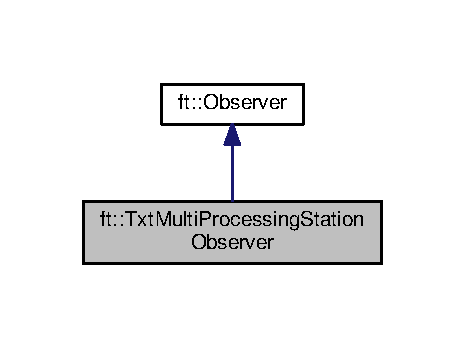
\includegraphics[width=223pt]{classft_1_1_txt_multi_processing_station_observer__inherit__graph}
\end{center}
\end{figure}


Collaboration diagram for ft\+:\+:Txt\+Multi\+Processing\+Station\+Observer\+:
\nopagebreak
\begin{figure}[H]
\begin{center}
\leavevmode
\includegraphics[width=223pt]{classft_1_1_txt_multi_processing_station_observer__coll__graph}
\end{center}
\end{figure}
\subsection*{Public Member Functions}
\begin{DoxyCompactItemize}
\item 
\hyperlink{classft_1_1_txt_multi_processing_station_observer_ab8bb2c64860c60ab17970c4f5ef9ca93}{Txt\+Multi\+Processing\+Station\+Observer} (\hyperlink{classft_1_1_txt_multi_processing_station}{ft\+::\+Txt\+Multi\+Processing\+Station} $\ast$s, \hyperlink{classft_1_1_txt_mqtt_factory_client}{ft\+::\+Txt\+Mqtt\+Factory\+Client} $\ast$mqttclient)
\item 
virtual \hyperlink{classft_1_1_txt_multi_processing_station_observer_a0b1f277448c1411848f6315967d93ae2}{$\sim$\+Txt\+Multi\+Processing\+Station\+Observer} ()
\item 
void \hyperlink{classft_1_1_txt_multi_processing_station_observer_aeddc4246174e6fd5aaa75823416c5e85}{Update} (\hyperlink{classft_1_1_subject_observer}{ft\+::\+Subject\+Observer} $\ast$the\+Changed\+Subject)
\end{DoxyCompactItemize}


\subsection{Constructor \& Destructor Documentation}
\index{ft\+::\+Txt\+Multi\+Processing\+Station\+Observer@{ft\+::\+Txt\+Multi\+Processing\+Station\+Observer}!Txt\+Multi\+Processing\+Station\+Observer@{Txt\+Multi\+Processing\+Station\+Observer}}
\index{Txt\+Multi\+Processing\+Station\+Observer@{Txt\+Multi\+Processing\+Station\+Observer}!ft\+::\+Txt\+Multi\+Processing\+Station\+Observer@{ft\+::\+Txt\+Multi\+Processing\+Station\+Observer}}
\subsubsection[{\texorpdfstring{Txt\+Multi\+Processing\+Station\+Observer(ft\+::\+Txt\+Multi\+Processing\+Station $\ast$s, ft\+::\+Txt\+Mqtt\+Factory\+Client $\ast$mqttclient)}{TxtMultiProcessingStationObserver(ft::TxtMultiProcessingStation *s, ft::TxtMqttFactoryClient *mqttclient)}}]{\setlength{\rightskip}{0pt plus 5cm}ft\+::\+Txt\+Multi\+Processing\+Station\+Observer\+::\+Txt\+Multi\+Processing\+Station\+Observer (
\begin{DoxyParamCaption}
\item[{{\bf ft\+::\+Txt\+Multi\+Processing\+Station} $\ast$}]{s, }
\item[{{\bf ft\+::\+Txt\+Mqtt\+Factory\+Client} $\ast$}]{mqttclient}
\end{DoxyParamCaption}
)\hspace{0.3cm}{\ttfamily [inline]}}\hypertarget{classft_1_1_txt_multi_processing_station_observer_ab8bb2c64860c60ab17970c4f5ef9ca93}{}\label{classft_1_1_txt_multi_processing_station_observer_ab8bb2c64860c60ab17970c4f5ef9ca93}
\index{ft\+::\+Txt\+Multi\+Processing\+Station\+Observer@{ft\+::\+Txt\+Multi\+Processing\+Station\+Observer}!````~Txt\+Multi\+Processing\+Station\+Observer@{$\sim$\+Txt\+Multi\+Processing\+Station\+Observer}}
\index{````~Txt\+Multi\+Processing\+Station\+Observer@{$\sim$\+Txt\+Multi\+Processing\+Station\+Observer}!ft\+::\+Txt\+Multi\+Processing\+Station\+Observer@{ft\+::\+Txt\+Multi\+Processing\+Station\+Observer}}
\subsubsection[{\texorpdfstring{$\sim$\+Txt\+Multi\+Processing\+Station\+Observer()}{~TxtMultiProcessingStationObserver()}}]{\setlength{\rightskip}{0pt plus 5cm}virtual ft\+::\+Txt\+Multi\+Processing\+Station\+Observer\+::$\sim$\+Txt\+Multi\+Processing\+Station\+Observer (
\begin{DoxyParamCaption}
{}
\end{DoxyParamCaption}
)\hspace{0.3cm}{\ttfamily [inline]}, {\ttfamily [virtual]}}\hypertarget{classft_1_1_txt_multi_processing_station_observer_a0b1f277448c1411848f6315967d93ae2}{}\label{classft_1_1_txt_multi_processing_station_observer_a0b1f277448c1411848f6315967d93ae2}


\subsection{Member Function Documentation}
\index{ft\+::\+Txt\+Multi\+Processing\+Station\+Observer@{ft\+::\+Txt\+Multi\+Processing\+Station\+Observer}!Update@{Update}}
\index{Update@{Update}!ft\+::\+Txt\+Multi\+Processing\+Station\+Observer@{ft\+::\+Txt\+Multi\+Processing\+Station\+Observer}}
\subsubsection[{\texorpdfstring{Update(ft\+::\+Subject\+Observer $\ast$the\+Changed\+Subject)}{Update(ft::SubjectObserver *theChangedSubject)}}]{\setlength{\rightskip}{0pt plus 5cm}void ft\+::\+Txt\+Multi\+Processing\+Station\+Observer\+::\+Update (
\begin{DoxyParamCaption}
\item[{{\bf ft\+::\+Subject\+Observer} $\ast$}]{the\+Changed\+Subject}
\end{DoxyParamCaption}
)\hspace{0.3cm}{\ttfamily [inline]}, {\ttfamily [virtual]}}\hypertarget{classft_1_1_txt_multi_processing_station_observer_aeddc4246174e6fd5aaa75823416c5e85}{}\label{classft_1_1_txt_multi_processing_station_observer_aeddc4246174e6fd5aaa75823416c5e85}


Implements \hyperlink{classft_1_1_observer_aeea41c77afbd09f595a4290954a5aa66}{ft\+::\+Observer}.



The documentation for this class was generated from the following file\+:\begin{DoxyCompactItemize}
\item 
\hyperlink{_txt_multi_processing_station_8h}{Txt\+Multi\+Processing\+Station.\+h}\end{DoxyCompactItemize}

\hypertarget{classft_1_1_txt_nfc_data}{}\section{ft\+:\+:Txt\+Nfc\+Data Class Reference}
\label{classft_1_1_txt_nfc_data}\index{ft\+::\+Txt\+Nfc\+Data@{ft\+::\+Txt\+Nfc\+Data}}


{\ttfamily \#include $<$Txt\+Nfc\+Device.\+h$>$}



Collaboration diagram for ft\+:\+:Txt\+Nfc\+Data\+:
\nopagebreak
\begin{figure}[H]
\begin{center}
\leavevmode
\includegraphics[width=234pt]{classft_1_1_txt_nfc_data__coll__graph}
\end{center}
\end{figure}
\subsection*{Public Member Functions}
\begin{DoxyCompactItemize}
\item 
\hyperlink{classft_1_1_txt_nfc_data_a2f52555bf6d581d5ae50ae38dddf51b4}{Txt\+Nfc\+Data} ()
\item 
virtual \hyperlink{classft_1_1_txt_nfc_data_a923f90a26428a0ea6c990545c2923dee}{$\sim$\+Txt\+Nfc\+Data} ()
\end{DoxyCompactItemize}
\subsection*{Public Attributes}
\begin{DoxyCompactItemize}
\item 
\hyperlink{classft_1_1_txt_workpiece}{Txt\+Workpiece} \hyperlink{classft_1_1_txt_nfc_data_aec7e3a438a5ff8f113f5c7819d038c1f}{wp}
\item 
\hyperlink{namespaceft_a6b29d191a4ff3cd5738bcb38e4392811}{u\+TS} \hyperlink{classft_1_1_txt_nfc_data_a7671b20d7d53b5be84267e61abd7ad98}{uts} \mbox{[}\hyperlink{_txt_nfc_device_8h_a4b7859088776a46f4866a6dc71689e6a}{N\+\_\+\+M\+A\+X\+\_\+\+TS}\mbox{]}
\item 
uint8\+\_\+t \hyperlink{classft_1_1_txt_nfc_data_a3ac76c3001f8142057d7784ef5bed85f}{mask\+\_\+ts}
\end{DoxyCompactItemize}


\subsection{Constructor \& Destructor Documentation}
\index{ft\+::\+Txt\+Nfc\+Data@{ft\+::\+Txt\+Nfc\+Data}!Txt\+Nfc\+Data@{Txt\+Nfc\+Data}}
\index{Txt\+Nfc\+Data@{Txt\+Nfc\+Data}!ft\+::\+Txt\+Nfc\+Data@{ft\+::\+Txt\+Nfc\+Data}}
\subsubsection[{\texorpdfstring{Txt\+Nfc\+Data()}{TxtNfcData()}}]{\setlength{\rightskip}{0pt plus 5cm}ft\+::\+Txt\+Nfc\+Data\+::\+Txt\+Nfc\+Data (
\begin{DoxyParamCaption}
{}
\end{DoxyParamCaption}
)\hspace{0.3cm}{\ttfamily [inline]}}\hypertarget{classft_1_1_txt_nfc_data_a2f52555bf6d581d5ae50ae38dddf51b4}{}\label{classft_1_1_txt_nfc_data_a2f52555bf6d581d5ae50ae38dddf51b4}
\index{ft\+::\+Txt\+Nfc\+Data@{ft\+::\+Txt\+Nfc\+Data}!````~Txt\+Nfc\+Data@{$\sim$\+Txt\+Nfc\+Data}}
\index{````~Txt\+Nfc\+Data@{$\sim$\+Txt\+Nfc\+Data}!ft\+::\+Txt\+Nfc\+Data@{ft\+::\+Txt\+Nfc\+Data}}
\subsubsection[{\texorpdfstring{$\sim$\+Txt\+Nfc\+Data()}{~TxtNfcData()}}]{\setlength{\rightskip}{0pt plus 5cm}virtual ft\+::\+Txt\+Nfc\+Data\+::$\sim$\+Txt\+Nfc\+Data (
\begin{DoxyParamCaption}
{}
\end{DoxyParamCaption}
)\hspace{0.3cm}{\ttfamily [inline]}, {\ttfamily [virtual]}}\hypertarget{classft_1_1_txt_nfc_data_a923f90a26428a0ea6c990545c2923dee}{}\label{classft_1_1_txt_nfc_data_a923f90a26428a0ea6c990545c2923dee}


\subsection{Member Data Documentation}
\index{ft\+::\+Txt\+Nfc\+Data@{ft\+::\+Txt\+Nfc\+Data}!mask\+\_\+ts@{mask\+\_\+ts}}
\index{mask\+\_\+ts@{mask\+\_\+ts}!ft\+::\+Txt\+Nfc\+Data@{ft\+::\+Txt\+Nfc\+Data}}
\subsubsection[{\texorpdfstring{mask\+\_\+ts}{mask_ts}}]{\setlength{\rightskip}{0pt plus 5cm}uint8\+\_\+t ft\+::\+Txt\+Nfc\+Data\+::mask\+\_\+ts}\hypertarget{classft_1_1_txt_nfc_data_a3ac76c3001f8142057d7784ef5bed85f}{}\label{classft_1_1_txt_nfc_data_a3ac76c3001f8142057d7784ef5bed85f}
\index{ft\+::\+Txt\+Nfc\+Data@{ft\+::\+Txt\+Nfc\+Data}!uts@{uts}}
\index{uts@{uts}!ft\+::\+Txt\+Nfc\+Data@{ft\+::\+Txt\+Nfc\+Data}}
\subsubsection[{\texorpdfstring{uts}{uts}}]{\setlength{\rightskip}{0pt plus 5cm}{\bf u\+TS} ft\+::\+Txt\+Nfc\+Data\+::uts\mbox{[}{\bf N\+\_\+\+M\+A\+X\+\_\+\+TS}\mbox{]}}\hypertarget{classft_1_1_txt_nfc_data_a7671b20d7d53b5be84267e61abd7ad98}{}\label{classft_1_1_txt_nfc_data_a7671b20d7d53b5be84267e61abd7ad98}
\index{ft\+::\+Txt\+Nfc\+Data@{ft\+::\+Txt\+Nfc\+Data}!wp@{wp}}
\index{wp@{wp}!ft\+::\+Txt\+Nfc\+Data@{ft\+::\+Txt\+Nfc\+Data}}
\subsubsection[{\texorpdfstring{wp}{wp}}]{\setlength{\rightskip}{0pt plus 5cm}{\bf Txt\+Workpiece} ft\+::\+Txt\+Nfc\+Data\+::wp}\hypertarget{classft_1_1_txt_nfc_data_aec7e3a438a5ff8f113f5c7819d038c1f}{}\label{classft_1_1_txt_nfc_data_aec7e3a438a5ff8f113f5c7819d038c1f}


The documentation for this class was generated from the following file\+:\begin{DoxyCompactItemize}
\item 
\hyperlink{_txt_nfc_device_8h}{Txt\+Nfc\+Device.\+h}\end{DoxyCompactItemize}

\hypertarget{classft_1_1_txt_nfc_device}{}\section{ft\+:\+:Txt\+Nfc\+Device Class Reference}
\label{classft_1_1_txt_nfc_device}\index{ft\+::\+Txt\+Nfc\+Device@{ft\+::\+Txt\+Nfc\+Device}}


{\ttfamily \#include $<$Txt\+Nfc\+Device.\+h$>$}



Inheritance diagram for ft\+:\+:Txt\+Nfc\+Device\+:
\nopagebreak
\begin{figure}[H]
\begin{center}
\leavevmode
\includegraphics[width=181pt]{classft_1_1_txt_nfc_device__inherit__graph}
\end{center}
\end{figure}


Collaboration diagram for ft\+:\+:Txt\+Nfc\+Device\+:
\nopagebreak
\begin{figure}[H]
\begin{center}
\leavevmode
\includegraphics[width=306pt]{classft_1_1_txt_nfc_device__coll__graph}
\end{center}
\end{figure}
\subsection*{Public Member Functions}
\begin{DoxyCompactItemize}
\item 
\hyperlink{classft_1_1_txt_nfc_device_ab5e9bb048da99db45ad5a666b2516887}{Txt\+Nfc\+Device} ()
\item 
virtual \hyperlink{classft_1_1_txt_nfc_device_a7b440f33260d269f870188cdb53f47e1}{$\sim$\+Txt\+Nfc\+Device} ()
\item 
bool \hyperlink{classft_1_1_txt_nfc_device_adfc7bf2b1fa487ed5af502d17b17c527}{open} ()
\item 
void \hyperlink{classft_1_1_txt_nfc_device_aec662a9e5128e5abee343bd8b9c09996}{close} ()
\item 
std\+::string \hyperlink{classft_1_1_txt_nfc_device_a49f1db0ef04655e2732f0726cc881abf}{read\+Tags\+Get\+U\+ID} ()
\item 
bool \hyperlink{classft_1_1_txt_nfc_device_adf81ce90e3613e8f17291fd6e3b5ed2e}{erase\+Tags} ()
\item 
std\+::string \hyperlink{classft_1_1_txt_nfc_device_a17f45d02a96db45a27aa82b6c5f48c24}{read\+Tags} ()
\item 
bool \hyperlink{classft_1_1_txt_nfc_device_abe33753d8d5ab511b6045b12399f1745}{write\+Tags} (\hyperlink{classft_1_1_txt_workpiece}{Txt\+Workpiece} wp, std\+::vector$<$ \hyperlink{namespaceft_a6b29d191a4ff3cd5738bcb38e4392811}{u\+TS} $>$ vuts, uint8\+\_\+t mask\+\_\+ts)
\item 
\hyperlink{classft_1_1_txt_nfc_data}{Txt\+Nfc\+Data} $\ast$ \hyperlink{classft_1_1_txt_nfc_device_ab7b821085cfb5459e7e234f25244d10d}{get\+Nfc\+Data} ()
\item 
void \hyperlink{classft_1_1_txt_nfc_device_aab6573c55e84cab2623d1eadd6f7cc28}{print\+Nfc\+Data} ()
\item 
void \hyperlink{classft_1_1_txt_nfc_device_ae7f154afa47b4e2010cd23e4b81a60b8}{publish} ()
\end{DoxyCompactItemize}
\subsection*{Protected Member Functions}
\begin{DoxyCompactItemize}
\item 
void \hyperlink{classft_1_1_txt_nfc_device_ad24e95c177354453f34ce9b4bae2bdb5}{print\+Raw\+Data} (uint8\+\_\+t $\ast$buffer)
\end{DoxyCompactItemize}
\subsection*{Protected Attributes}
\begin{DoxyCompactItemize}
\item 
bool \hyperlink{classft_1_1_txt_nfc_device_a41320e73fee7719850232c9c276f26b1}{opened}
\item 
nfc\+\_\+device $\ast$ \hyperlink{classft_1_1_txt_nfc_device_a59bf44e5cdecb9619cb151ac0dbdd4c4}{pnd}
\item 
nfc\+\_\+context $\ast$ \hyperlink{classft_1_1_txt_nfc_device_a38f93ed8b4c00b8d25903f93bdcfb309}{context}
\item 
\hyperlink{classft_1_1_txt_nfc_data}{Txt\+Nfc\+Data} $\ast$ \hyperlink{classft_1_1_txt_nfc_device_ab5b73197e3759749a26d0a73b7fb07a3}{nfc\+Data}
\end{DoxyCompactItemize}


\subsection{Constructor \& Destructor Documentation}
\index{ft\+::\+Txt\+Nfc\+Device@{ft\+::\+Txt\+Nfc\+Device}!Txt\+Nfc\+Device@{Txt\+Nfc\+Device}}
\index{Txt\+Nfc\+Device@{Txt\+Nfc\+Device}!ft\+::\+Txt\+Nfc\+Device@{ft\+::\+Txt\+Nfc\+Device}}
\subsubsection[{\texorpdfstring{Txt\+Nfc\+Device()}{TxtNfcDevice()}}]{\setlength{\rightskip}{0pt plus 5cm}ft\+::\+Txt\+Nfc\+Device\+::\+Txt\+Nfc\+Device (
\begin{DoxyParamCaption}
{}
\end{DoxyParamCaption}
)}\hypertarget{classft_1_1_txt_nfc_device_ab5e9bb048da99db45ad5a666b2516887}{}\label{classft_1_1_txt_nfc_device_ab5e9bb048da99db45ad5a666b2516887}
\index{ft\+::\+Txt\+Nfc\+Device@{ft\+::\+Txt\+Nfc\+Device}!````~Txt\+Nfc\+Device@{$\sim$\+Txt\+Nfc\+Device}}
\index{````~Txt\+Nfc\+Device@{$\sim$\+Txt\+Nfc\+Device}!ft\+::\+Txt\+Nfc\+Device@{ft\+::\+Txt\+Nfc\+Device}}
\subsubsection[{\texorpdfstring{$\sim$\+Txt\+Nfc\+Device()}{~TxtNfcDevice()}}]{\setlength{\rightskip}{0pt plus 5cm}virtual ft\+::\+Txt\+Nfc\+Device\+::$\sim$\+Txt\+Nfc\+Device (
\begin{DoxyParamCaption}
{}
\end{DoxyParamCaption}
)\hspace{0.3cm}{\ttfamily [virtual]}}\hypertarget{classft_1_1_txt_nfc_device_a7b440f33260d269f870188cdb53f47e1}{}\label{classft_1_1_txt_nfc_device_a7b440f33260d269f870188cdb53f47e1}


\subsection{Member Function Documentation}
\index{ft\+::\+Txt\+Nfc\+Device@{ft\+::\+Txt\+Nfc\+Device}!close@{close}}
\index{close@{close}!ft\+::\+Txt\+Nfc\+Device@{ft\+::\+Txt\+Nfc\+Device}}
\subsubsection[{\texorpdfstring{close()}{close()}}]{\setlength{\rightskip}{0pt plus 5cm}void ft\+::\+Txt\+Nfc\+Device\+::close (
\begin{DoxyParamCaption}
{}
\end{DoxyParamCaption}
)}\hypertarget{classft_1_1_txt_nfc_device_aec662a9e5128e5abee343bd8b9c09996}{}\label{classft_1_1_txt_nfc_device_aec662a9e5128e5abee343bd8b9c09996}
\index{ft\+::\+Txt\+Nfc\+Device@{ft\+::\+Txt\+Nfc\+Device}!erase\+Tags@{erase\+Tags}}
\index{erase\+Tags@{erase\+Tags}!ft\+::\+Txt\+Nfc\+Device@{ft\+::\+Txt\+Nfc\+Device}}
\subsubsection[{\texorpdfstring{erase\+Tags()}{eraseTags()}}]{\setlength{\rightskip}{0pt plus 5cm}bool ft\+::\+Txt\+Nfc\+Device\+::erase\+Tags (
\begin{DoxyParamCaption}
{}
\end{DoxyParamCaption}
)}\hypertarget{classft_1_1_txt_nfc_device_adf81ce90e3613e8f17291fd6e3b5ed2e}{}\label{classft_1_1_txt_nfc_device_adf81ce90e3613e8f17291fd6e3b5ed2e}
\index{ft\+::\+Txt\+Nfc\+Device@{ft\+::\+Txt\+Nfc\+Device}!get\+Nfc\+Data@{get\+Nfc\+Data}}
\index{get\+Nfc\+Data@{get\+Nfc\+Data}!ft\+::\+Txt\+Nfc\+Device@{ft\+::\+Txt\+Nfc\+Device}}
\subsubsection[{\texorpdfstring{get\+Nfc\+Data()}{getNfcData()}}]{\setlength{\rightskip}{0pt plus 5cm}{\bf Txt\+Nfc\+Data}$\ast$ ft\+::\+Txt\+Nfc\+Device\+::get\+Nfc\+Data (
\begin{DoxyParamCaption}
{}
\end{DoxyParamCaption}
)\hspace{0.3cm}{\ttfamily [inline]}}\hypertarget{classft_1_1_txt_nfc_device_ab7b821085cfb5459e7e234f25244d10d}{}\label{classft_1_1_txt_nfc_device_ab7b821085cfb5459e7e234f25244d10d}
\index{ft\+::\+Txt\+Nfc\+Device@{ft\+::\+Txt\+Nfc\+Device}!open@{open}}
\index{open@{open}!ft\+::\+Txt\+Nfc\+Device@{ft\+::\+Txt\+Nfc\+Device}}
\subsubsection[{\texorpdfstring{open()}{open()}}]{\setlength{\rightskip}{0pt plus 5cm}bool ft\+::\+Txt\+Nfc\+Device\+::open (
\begin{DoxyParamCaption}
{}
\end{DoxyParamCaption}
)}\hypertarget{classft_1_1_txt_nfc_device_adfc7bf2b1fa487ed5af502d17b17c527}{}\label{classft_1_1_txt_nfc_device_adfc7bf2b1fa487ed5af502d17b17c527}
\index{ft\+::\+Txt\+Nfc\+Device@{ft\+::\+Txt\+Nfc\+Device}!print\+Nfc\+Data@{print\+Nfc\+Data}}
\index{print\+Nfc\+Data@{print\+Nfc\+Data}!ft\+::\+Txt\+Nfc\+Device@{ft\+::\+Txt\+Nfc\+Device}}
\subsubsection[{\texorpdfstring{print\+Nfc\+Data()}{printNfcData()}}]{\setlength{\rightskip}{0pt plus 5cm}void ft\+::\+Txt\+Nfc\+Device\+::print\+Nfc\+Data (
\begin{DoxyParamCaption}
{}
\end{DoxyParamCaption}
)}\hypertarget{classft_1_1_txt_nfc_device_aab6573c55e84cab2623d1eadd6f7cc28}{}\label{classft_1_1_txt_nfc_device_aab6573c55e84cab2623d1eadd6f7cc28}
\index{ft\+::\+Txt\+Nfc\+Device@{ft\+::\+Txt\+Nfc\+Device}!print\+Raw\+Data@{print\+Raw\+Data}}
\index{print\+Raw\+Data@{print\+Raw\+Data}!ft\+::\+Txt\+Nfc\+Device@{ft\+::\+Txt\+Nfc\+Device}}
\subsubsection[{\texorpdfstring{print\+Raw\+Data(uint8\+\_\+t $\ast$buffer)}{printRawData(uint8_t *buffer)}}]{\setlength{\rightskip}{0pt plus 5cm}void ft\+::\+Txt\+Nfc\+Device\+::print\+Raw\+Data (
\begin{DoxyParamCaption}
\item[{uint8\+\_\+t $\ast$}]{buffer}
\end{DoxyParamCaption}
)\hspace{0.3cm}{\ttfamily [protected]}}\hypertarget{classft_1_1_txt_nfc_device_ad24e95c177354453f34ce9b4bae2bdb5}{}\label{classft_1_1_txt_nfc_device_ad24e95c177354453f34ce9b4bae2bdb5}
\index{ft\+::\+Txt\+Nfc\+Device@{ft\+::\+Txt\+Nfc\+Device}!publish@{publish}}
\index{publish@{publish}!ft\+::\+Txt\+Nfc\+Device@{ft\+::\+Txt\+Nfc\+Device}}
\subsubsection[{\texorpdfstring{publish()}{publish()}}]{\setlength{\rightskip}{0pt plus 5cm}void ft\+::\+Txt\+Nfc\+Device\+::publish (
\begin{DoxyParamCaption}
{}
\end{DoxyParamCaption}
)\hspace{0.3cm}{\ttfamily [inline]}}\hypertarget{classft_1_1_txt_nfc_device_ae7f154afa47b4e2010cd23e4b81a60b8}{}\label{classft_1_1_txt_nfc_device_ae7f154afa47b4e2010cd23e4b81a60b8}
\index{ft\+::\+Txt\+Nfc\+Device@{ft\+::\+Txt\+Nfc\+Device}!read\+Tags@{read\+Tags}}
\index{read\+Tags@{read\+Tags}!ft\+::\+Txt\+Nfc\+Device@{ft\+::\+Txt\+Nfc\+Device}}
\subsubsection[{\texorpdfstring{read\+Tags()}{readTags()}}]{\setlength{\rightskip}{0pt plus 5cm}std\+::string ft\+::\+Txt\+Nfc\+Device\+::read\+Tags (
\begin{DoxyParamCaption}
{}
\end{DoxyParamCaption}
)}\hypertarget{classft_1_1_txt_nfc_device_a17f45d02a96db45a27aa82b6c5f48c24}{}\label{classft_1_1_txt_nfc_device_a17f45d02a96db45a27aa82b6c5f48c24}
\index{ft\+::\+Txt\+Nfc\+Device@{ft\+::\+Txt\+Nfc\+Device}!read\+Tags\+Get\+U\+ID@{read\+Tags\+Get\+U\+ID}}
\index{read\+Tags\+Get\+U\+ID@{read\+Tags\+Get\+U\+ID}!ft\+::\+Txt\+Nfc\+Device@{ft\+::\+Txt\+Nfc\+Device}}
\subsubsection[{\texorpdfstring{read\+Tags\+Get\+U\+I\+D()}{readTagsGetUID()}}]{\setlength{\rightskip}{0pt plus 5cm}std\+::string ft\+::\+Txt\+Nfc\+Device\+::read\+Tags\+Get\+U\+ID (
\begin{DoxyParamCaption}
{}
\end{DoxyParamCaption}
)}\hypertarget{classft_1_1_txt_nfc_device_a49f1db0ef04655e2732f0726cc881abf}{}\label{classft_1_1_txt_nfc_device_a49f1db0ef04655e2732f0726cc881abf}
\index{ft\+::\+Txt\+Nfc\+Device@{ft\+::\+Txt\+Nfc\+Device}!write\+Tags@{write\+Tags}}
\index{write\+Tags@{write\+Tags}!ft\+::\+Txt\+Nfc\+Device@{ft\+::\+Txt\+Nfc\+Device}}
\subsubsection[{\texorpdfstring{write\+Tags(\+Txt\+Workpiece wp, std\+::vector$<$ u\+T\+S $>$ vuts, uint8\+\_\+t mask\+\_\+ts)}{writeTags(TxtWorkpiece wp, std::vector< uTS > vuts, uint8_t mask_ts)}}]{\setlength{\rightskip}{0pt plus 5cm}bool ft\+::\+Txt\+Nfc\+Device\+::write\+Tags (
\begin{DoxyParamCaption}
\item[{{\bf Txt\+Workpiece}}]{wp, }
\item[{std\+::vector$<$ {\bf u\+TS} $>$}]{vuts, }
\item[{uint8\+\_\+t}]{mask\+\_\+ts}
\end{DoxyParamCaption}
)}\hypertarget{classft_1_1_txt_nfc_device_abe33753d8d5ab511b6045b12399f1745}{}\label{classft_1_1_txt_nfc_device_abe33753d8d5ab511b6045b12399f1745}


\subsection{Member Data Documentation}
\index{ft\+::\+Txt\+Nfc\+Device@{ft\+::\+Txt\+Nfc\+Device}!context@{context}}
\index{context@{context}!ft\+::\+Txt\+Nfc\+Device@{ft\+::\+Txt\+Nfc\+Device}}
\subsubsection[{\texorpdfstring{context}{context}}]{\setlength{\rightskip}{0pt plus 5cm}nfc\+\_\+context$\ast$ ft\+::\+Txt\+Nfc\+Device\+::context\hspace{0.3cm}{\ttfamily [protected]}}\hypertarget{classft_1_1_txt_nfc_device_a38f93ed8b4c00b8d25903f93bdcfb309}{}\label{classft_1_1_txt_nfc_device_a38f93ed8b4c00b8d25903f93bdcfb309}
\index{ft\+::\+Txt\+Nfc\+Device@{ft\+::\+Txt\+Nfc\+Device}!nfc\+Data@{nfc\+Data}}
\index{nfc\+Data@{nfc\+Data}!ft\+::\+Txt\+Nfc\+Device@{ft\+::\+Txt\+Nfc\+Device}}
\subsubsection[{\texorpdfstring{nfc\+Data}{nfcData}}]{\setlength{\rightskip}{0pt plus 5cm}{\bf Txt\+Nfc\+Data}$\ast$ ft\+::\+Txt\+Nfc\+Device\+::nfc\+Data\hspace{0.3cm}{\ttfamily [protected]}}\hypertarget{classft_1_1_txt_nfc_device_ab5b73197e3759749a26d0a73b7fb07a3}{}\label{classft_1_1_txt_nfc_device_ab5b73197e3759749a26d0a73b7fb07a3}
\index{ft\+::\+Txt\+Nfc\+Device@{ft\+::\+Txt\+Nfc\+Device}!opened@{opened}}
\index{opened@{opened}!ft\+::\+Txt\+Nfc\+Device@{ft\+::\+Txt\+Nfc\+Device}}
\subsubsection[{\texorpdfstring{opened}{opened}}]{\setlength{\rightskip}{0pt plus 5cm}bool ft\+::\+Txt\+Nfc\+Device\+::opened\hspace{0.3cm}{\ttfamily [protected]}}\hypertarget{classft_1_1_txt_nfc_device_a41320e73fee7719850232c9c276f26b1}{}\label{classft_1_1_txt_nfc_device_a41320e73fee7719850232c9c276f26b1}
\index{ft\+::\+Txt\+Nfc\+Device@{ft\+::\+Txt\+Nfc\+Device}!pnd@{pnd}}
\index{pnd@{pnd}!ft\+::\+Txt\+Nfc\+Device@{ft\+::\+Txt\+Nfc\+Device}}
\subsubsection[{\texorpdfstring{pnd}{pnd}}]{\setlength{\rightskip}{0pt plus 5cm}nfc\+\_\+device$\ast$ ft\+::\+Txt\+Nfc\+Device\+::pnd\hspace{0.3cm}{\ttfamily [protected]}}\hypertarget{classft_1_1_txt_nfc_device_a59bf44e5cdecb9619cb151ac0dbdd4c4}{}\label{classft_1_1_txt_nfc_device_a59bf44e5cdecb9619cb151ac0dbdd4c4}


The documentation for this class was generated from the following file\+:\begin{DoxyCompactItemize}
\item 
\hyperlink{_txt_nfc_device_8h}{Txt\+Nfc\+Device.\+h}\end{DoxyCompactItemize}

\hypertarget{classft_1_1_txt_nfc_device_observer}{}\section{ft\+:\+:Txt\+Nfc\+Device\+Observer Class Reference}
\label{classft_1_1_txt_nfc_device_observer}\index{ft\+::\+Txt\+Nfc\+Device\+Observer@{ft\+::\+Txt\+Nfc\+Device\+Observer}}


{\ttfamily \#include $<$Txt\+Nfc\+Device.\+h$>$}



Inheritance diagram for ft\+:\+:Txt\+Nfc\+Device\+Observer\+:
\nopagebreak
\begin{figure}[H]
\begin{center}
\leavevmode
\includegraphics[width=209pt]{classft_1_1_txt_nfc_device_observer__inherit__graph}
\end{center}
\end{figure}


Collaboration diagram for ft\+:\+:Txt\+Nfc\+Device\+Observer\+:
\nopagebreak
\begin{figure}[H]
\begin{center}
\leavevmode
\includegraphics[width=209pt]{classft_1_1_txt_nfc_device_observer__coll__graph}
\end{center}
\end{figure}
\subsection*{Public Member Functions}
\begin{DoxyCompactItemize}
\item 
\hyperlink{classft_1_1_txt_nfc_device_observer_a94125d4c52d11540c2a729e3614ab957}{Txt\+Nfc\+Device\+Observer} (\hyperlink{classft_1_1_txt_nfc_device}{ft\+::\+Txt\+Nfc\+Device} $\ast$s, \hyperlink{classft_1_1_txt_mqtt_factory_client}{ft\+::\+Txt\+Mqtt\+Factory\+Client} $\ast$mqttclient)
\item 
virtual \hyperlink{classft_1_1_txt_nfc_device_observer_a331263b07cc20d502b1154e467eef139}{$\sim$\+Txt\+Nfc\+Device\+Observer} ()
\item 
void \hyperlink{classft_1_1_txt_nfc_device_observer_a32311fe745e0777842453ef8b93083b8}{Update} (\hyperlink{classft_1_1_subject_observer}{ft\+::\+Subject\+Observer} $\ast$the\+Changed\+Subject)
\end{DoxyCompactItemize}


\subsection{Constructor \& Destructor Documentation}
\index{ft\+::\+Txt\+Nfc\+Device\+Observer@{ft\+::\+Txt\+Nfc\+Device\+Observer}!Txt\+Nfc\+Device\+Observer@{Txt\+Nfc\+Device\+Observer}}
\index{Txt\+Nfc\+Device\+Observer@{Txt\+Nfc\+Device\+Observer}!ft\+::\+Txt\+Nfc\+Device\+Observer@{ft\+::\+Txt\+Nfc\+Device\+Observer}}
\subsubsection[{\texorpdfstring{Txt\+Nfc\+Device\+Observer(ft\+::\+Txt\+Nfc\+Device $\ast$s, ft\+::\+Txt\+Mqtt\+Factory\+Client $\ast$mqttclient)}{TxtNfcDeviceObserver(ft::TxtNfcDevice *s, ft::TxtMqttFactoryClient *mqttclient)}}]{\setlength{\rightskip}{0pt plus 5cm}ft\+::\+Txt\+Nfc\+Device\+Observer\+::\+Txt\+Nfc\+Device\+Observer (
\begin{DoxyParamCaption}
\item[{{\bf ft\+::\+Txt\+Nfc\+Device} $\ast$}]{s, }
\item[{{\bf ft\+::\+Txt\+Mqtt\+Factory\+Client} $\ast$}]{mqttclient}
\end{DoxyParamCaption}
)\hspace{0.3cm}{\ttfamily [inline]}}\hypertarget{classft_1_1_txt_nfc_device_observer_a94125d4c52d11540c2a729e3614ab957}{}\label{classft_1_1_txt_nfc_device_observer_a94125d4c52d11540c2a729e3614ab957}
\index{ft\+::\+Txt\+Nfc\+Device\+Observer@{ft\+::\+Txt\+Nfc\+Device\+Observer}!````~Txt\+Nfc\+Device\+Observer@{$\sim$\+Txt\+Nfc\+Device\+Observer}}
\index{````~Txt\+Nfc\+Device\+Observer@{$\sim$\+Txt\+Nfc\+Device\+Observer}!ft\+::\+Txt\+Nfc\+Device\+Observer@{ft\+::\+Txt\+Nfc\+Device\+Observer}}
\subsubsection[{\texorpdfstring{$\sim$\+Txt\+Nfc\+Device\+Observer()}{~TxtNfcDeviceObserver()}}]{\setlength{\rightskip}{0pt plus 5cm}virtual ft\+::\+Txt\+Nfc\+Device\+Observer\+::$\sim$\+Txt\+Nfc\+Device\+Observer (
\begin{DoxyParamCaption}
{}
\end{DoxyParamCaption}
)\hspace{0.3cm}{\ttfamily [inline]}, {\ttfamily [virtual]}}\hypertarget{classft_1_1_txt_nfc_device_observer_a331263b07cc20d502b1154e467eef139}{}\label{classft_1_1_txt_nfc_device_observer_a331263b07cc20d502b1154e467eef139}


\subsection{Member Function Documentation}
\index{ft\+::\+Txt\+Nfc\+Device\+Observer@{ft\+::\+Txt\+Nfc\+Device\+Observer}!Update@{Update}}
\index{Update@{Update}!ft\+::\+Txt\+Nfc\+Device\+Observer@{ft\+::\+Txt\+Nfc\+Device\+Observer}}
\subsubsection[{\texorpdfstring{Update(ft\+::\+Subject\+Observer $\ast$the\+Changed\+Subject)}{Update(ft::SubjectObserver *theChangedSubject)}}]{\setlength{\rightskip}{0pt plus 5cm}void ft\+::\+Txt\+Nfc\+Device\+Observer\+::\+Update (
\begin{DoxyParamCaption}
\item[{{\bf ft\+::\+Subject\+Observer} $\ast$}]{the\+Changed\+Subject}
\end{DoxyParamCaption}
)\hspace{0.3cm}{\ttfamily [inline]}, {\ttfamily [virtual]}}\hypertarget{classft_1_1_txt_nfc_device_observer_a32311fe745e0777842453ef8b93083b8}{}\label{classft_1_1_txt_nfc_device_observer_a32311fe745e0777842453ef8b93083b8}


Implements \hyperlink{classft_1_1_observer_aeea41c77afbd09f595a4290954a5aa66}{ft\+::\+Observer}.



The documentation for this class was generated from the following file\+:\begin{DoxyCompactItemize}
\item 
\hyperlink{_txt_nfc_device_8h}{Txt\+Nfc\+Device.\+h}\end{DoxyCompactItemize}

\hypertarget{structft_1_1_txt_order_state}{}\section{ft\+:\+:Txt\+Order\+State Struct Reference}
\label{structft_1_1_txt_order_state}\index{ft\+::\+Txt\+Order\+State@{ft\+::\+Txt\+Order\+State}}


{\ttfamily \#include $<$Txt\+Factory\+Types.\+h$>$}

\subsection*{Public Attributes}
\begin{DoxyCompactItemize}
\item 
\hyperlink{namespaceft_a2d5bf01b2da29de3c061682f3195b5b2}{Txt\+W\+P\+Type\+\_\+t} \hyperlink{structft_1_1_txt_order_state_a52dbd5afe5eafa36d1892bd66514dd2a}{type}
\item 
\hyperlink{namespaceft_a0b621af47c2875bbecb5f4a3d4218a5c}{Txt\+Order\+State\+\_\+t} \hyperlink{structft_1_1_txt_order_state_a2d088544a4d9a5213db0bd3d6f4d89de}{state}
\end{DoxyCompactItemize}


\subsection{Member Data Documentation}
\index{ft\+::\+Txt\+Order\+State@{ft\+::\+Txt\+Order\+State}!state@{state}}
\index{state@{state}!ft\+::\+Txt\+Order\+State@{ft\+::\+Txt\+Order\+State}}
\subsubsection[{\texorpdfstring{state}{state}}]{\setlength{\rightskip}{0pt plus 5cm}{\bf Txt\+Order\+State\+\_\+t} ft\+::\+Txt\+Order\+State\+::state}\hypertarget{structft_1_1_txt_order_state_a2d088544a4d9a5213db0bd3d6f4d89de}{}\label{structft_1_1_txt_order_state_a2d088544a4d9a5213db0bd3d6f4d89de}
\index{ft\+::\+Txt\+Order\+State@{ft\+::\+Txt\+Order\+State}!type@{type}}
\index{type@{type}!ft\+::\+Txt\+Order\+State@{ft\+::\+Txt\+Order\+State}}
\subsubsection[{\texorpdfstring{type}{type}}]{\setlength{\rightskip}{0pt plus 5cm}{\bf Txt\+W\+P\+Type\+\_\+t} ft\+::\+Txt\+Order\+State\+::type}\hypertarget{structft_1_1_txt_order_state_a52dbd5afe5eafa36d1892bd66514dd2a}{}\label{structft_1_1_txt_order_state_a52dbd5afe5eafa36d1892bd66514dd2a}


The documentation for this struct was generated from the following file\+:\begin{DoxyCompactItemize}
\item 
\hyperlink{_txt_factory_types_8h}{Txt\+Factory\+Types.\+h}\end{DoxyCompactItemize}

\hypertarget{classft_1_1_txt_pan_tilt_unit}{}\section{ft\+:\+:Txt\+Pan\+Tilt\+Unit Class Reference}
\label{classft_1_1_txt_pan_tilt_unit}\index{ft\+::\+Txt\+Pan\+Tilt\+Unit@{ft\+::\+Txt\+Pan\+Tilt\+Unit}}


{\ttfamily \#include $<$Txt\+Pan\+Tilt\+Unit.\+h$>$}



Inheritance diagram for ft\+:\+:Txt\+Pan\+Tilt\+Unit\+:
\nopagebreak
\begin{figure}[H]
\begin{center}
\leavevmode
\includegraphics[width=181pt]{classft_1_1_txt_pan_tilt_unit__inherit__graph}
\end{center}
\end{figure}


Collaboration diagram for ft\+:\+:Txt\+Pan\+Tilt\+Unit\+:
\nopagebreak
\begin{figure}[H]
\begin{center}
\leavevmode
\includegraphics[width=334pt]{classft_1_1_txt_pan_tilt_unit__coll__graph}
\end{center}
\end{figure}
\subsection*{Public Member Functions}
\begin{DoxyCompactItemize}
\item 
\hyperlink{classft_1_1_txt_pan_tilt_unit_a751edaac373d0e0e860dc2f8c2c4c282}{Txt\+Pan\+Tilt\+Unit} (F\+I\+S\+H\+\_\+\+X1\+\_\+\+T\+R\+A\+N\+S\+F\+ER $\ast$\hyperlink{classft_1_1_txt_pan_tilt_unit_a0980755f4b1e238ff65ce3799133a1cd}{p\+T\+Area}, uint8\+\_\+t \hyperlink{classft_1_1_txt_pan_tilt_unit_a1a565a8918d7e9ca3dd33280a20c32dc}{ch\+Pan}=0, uint8\+\_\+t \hyperlink{classft_1_1_txt_pan_tilt_unit_acddd9fc227b70c060fb5816870677101}{ch\+Tilt}=1)
\item 
virtual \hyperlink{classft_1_1_txt_pan_tilt_unit_a94f6d6ffcf28ca4dd2dc52a507656409}{$\sim$\+Txt\+Pan\+Tilt\+Unit} ()
\item 
bool \hyperlink{classft_1_1_txt_pan_tilt_unit_abc56d932cec09c497a6a803d21f296de}{init} ()
\item 
\hyperlink{namespaceft_aaf50a06f05b9188eeec535212b261df0}{Txt\+Pan\+Tilt\+Unit\+\_\+status\+\_\+t} \hyperlink{classft_1_1_txt_pan_tilt_unit_a2dd82f8f2af4844498773aa039e33ca1}{get\+Status} ()
\item 
void \hyperlink{classft_1_1_txt_pan_tilt_unit_a5afa571e04da333164a4b372c242064b}{set\+Step\+Pan} (uint16\+\_\+t steps)
\item 
void \hyperlink{classft_1_1_txt_pan_tilt_unit_a317eb98f588ecff30289880bd0175d13}{set\+Step\+Tilt} (uint16\+\_\+t steps)
\item 
uint16\+\_\+t \hyperlink{classft_1_1_txt_pan_tilt_unit_a63fbb66a26974f73726168782db3bb07}{get\+Step\+Pan} ()
\item 
uint16\+\_\+t \hyperlink{classft_1_1_txt_pan_tilt_unit_acecf4cc15094fbf0bbe5f9d69b972846}{get\+Step\+Tilt} ()
\item 
void \hyperlink{classft_1_1_txt_pan_tilt_unit_af8e93c217fc34a2f5b56b22fd9442553}{set\+Speed\+Pan} (int16\+\_\+t speed)
\item 
void \hyperlink{classft_1_1_txt_pan_tilt_unit_a44d7dc0b533907ff1e475cffde4c3f5c}{set\+Speed\+Tilt} (int16\+\_\+t speed)
\item 
int16\+\_\+t \hyperlink{classft_1_1_txt_pan_tilt_unit_ad7dcae4da1224cab6c2bb50698abb83e}{get\+Speed\+Pan} ()
\item 
int16\+\_\+t \hyperlink{classft_1_1_txt_pan_tilt_unit_a445c47c5d67d0226c91d08567c2e14c0}{get\+Speed\+Tilt} ()
\item 
uint16\+\_\+t \hyperlink{classft_1_1_txt_pan_tilt_unit_a868812a59fb144a940c33d80133fc1c3}{get\+Pos\+Pan} ()
\item 
uint16\+\_\+t \hyperlink{classft_1_1_txt_pan_tilt_unit_a12d225cc056a07264df2f299513d3817}{get\+Pos\+Tilt} ()
\item 
float \hyperlink{classft_1_1_txt_pan_tilt_unit_a5cf016f88fffb4b12deaf184471fb571}{get\+Pos\+Pan\+Rel} ()
\item 
float \hyperlink{classft_1_1_txt_pan_tilt_unit_a2ff2da2bf36eb344e7281a2c45589f8b}{get\+Pos\+Tilt\+Rel} ()
\item 
void \hyperlink{classft_1_1_txt_pan_tilt_unit_a53db85ecbf3a4ca80d1197d8cb749625}{stop} ()
\item 
bool \hyperlink{classft_1_1_txt_pan_tilt_unit_adcb3f29ea47c30b2ce6dacafbe67fbef}{move\+Pos} (uint16\+\_\+t p\+Pan, uint16\+\_\+t p\+Tilt)
\item 
bool \hyperlink{classft_1_1_txt_pan_tilt_unit_ab50b506049d75fdf9cf1eea63bbba5b8}{move\+Center} ()
\item 
bool \hyperlink{classft_1_1_txt_pan_tilt_unit_a2502ef5731162177c2f90b7ddb4ec9cb}{move\+H\+BW} ()
\item 
void \hyperlink{classft_1_1_txt_pan_tilt_unit_aa4559d36c19193efce7fc64edb310194}{move\+Home} ()
\item 
void \hyperlink{classft_1_1_txt_pan_tilt_unit_a1513c7f1bfede9d6c2eda1501c195b78}{move\+Pan0} ()
\item 
void \hyperlink{classft_1_1_txt_pan_tilt_unit_a6d2a6b7b803a2263c915ca0545f89146}{move\+Pan\+Center} ()
\item 
void \hyperlink{classft_1_1_txt_pan_tilt_unit_a512c8430f27cae174e489fbf78e0f834}{move\+Pan\+End} ()
\item 
void \hyperlink{classft_1_1_txt_pan_tilt_unit_a906c2b58e965e1d9c0f1f0f6b0395c10}{move\+Tilt0} ()
\item 
void \hyperlink{classft_1_1_txt_pan_tilt_unit_ad2916df64a2a732a3bbe338e6d559f5e}{move\+Tilt\+Center} ()
\item 
void \hyperlink{classft_1_1_txt_pan_tilt_unit_a21f29747defca1c702146dd90b7e6441}{move\+Tilt\+End} ()
\item 
void \hyperlink{classft_1_1_txt_pan_tilt_unit_a31c69da70a912f62ea51ac8fb7167aa9}{move\+Step\+Pan\+Left} ()
\item 
void \hyperlink{classft_1_1_txt_pan_tilt_unit_a5330e54d284bd1de523fcc6cf93082e0}{move\+Step\+Pan\+Right} ()
\item 
void \hyperlink{classft_1_1_txt_pan_tilt_unit_a329beb715169e44e1c9a1d14a327bafd}{move\+Step\+Tilt\+Up} ()
\item 
void \hyperlink{classft_1_1_txt_pan_tilt_unit_aa7e4a9750b06e014956f63fd3b5fac35}{move\+Step\+Tilt\+Down} ()
\end{DoxyCompactItemize}
\subsection*{Protected Member Functions}
\begin{DoxyCompactItemize}
\item 
void \hyperlink{classft_1_1_txt_pan_tilt_unit_a10a3340d1175128af17600aee6d208f5}{set\+Motors\+Off} ()
\item 
void \hyperlink{classft_1_1_txt_pan_tilt_unit_aa6e90052736e2260d5336e6e45625790}{set\+Motor\+Pan\+Off} ()
\item 
void \hyperlink{classft_1_1_txt_pan_tilt_unit_ae60c0c9c8e5a9f12b527d9c5c6c01e21}{set\+Motor\+Tilt\+Off} ()
\item 
void \hyperlink{classft_1_1_txt_pan_tilt_unit_a592992fb1f782c3a85bf43b2b812d1c1}{move\+Left} (uint8\+\_\+t ch, uint16\+\_\+t steps, int16\+\_\+t speed, uint16\+\_\+t $\ast$p\+Pos, uint16\+\_\+t pos\+End)
\item 
void \hyperlink{classft_1_1_txt_pan_tilt_unit_a6d00615d078b7fe284b08c50214ea9e8}{move\+Right} (uint8\+\_\+t ch, uint16\+\_\+t steps, int16\+\_\+t speed, uint16\+\_\+t $\ast$p\+Pos, uint16\+\_\+t pos\+End)
\item 
void \hyperlink{classft_1_1_txt_pan_tilt_unit_a947bff817236114544e5577d56c115b5}{move\+Pan\+Left} (uint16\+\_\+t steps)
\item 
void \hyperlink{classft_1_1_txt_pan_tilt_unit_ab44bf3e2be81f6d26a0dfc8f6f2b6483}{move\+Pan\+Right} (uint16\+\_\+t steps)
\item 
void \hyperlink{classft_1_1_txt_pan_tilt_unit_a8be0f85e285a511400a1e08f2dac2e26}{move\+Tilt\+Up} (uint16\+\_\+t steps)
\item 
void \hyperlink{classft_1_1_txt_pan_tilt_unit_a3e9951fe1f76c86af5ddf8c87d90d207}{move\+Tilt\+Down} (uint16\+\_\+t steps)
\item 
bool \hyperlink{classft_1_1_txt_pan_tilt_unit_a9439fd5d93222860f035d5c672d68573}{move\+Pan\+Pos} (uint16\+\_\+t p\+Pan)
\item 
bool \hyperlink{classft_1_1_txt_pan_tilt_unit_aead89c4a30fab6c23126e88b71caf943}{move\+Tilt\+Pos} (uint16\+\_\+t p\+Tilt)
\end{DoxyCompactItemize}
\subsection*{Protected Attributes}
\begin{DoxyCompactItemize}
\item 
F\+I\+S\+H\+\_\+\+X1\+\_\+\+T\+R\+A\+N\+S\+F\+ER $\ast$ \hyperlink{classft_1_1_txt_pan_tilt_unit_a0980755f4b1e238ff65ce3799133a1cd}{p\+T\+Area}
\item 
bool \hyperlink{classft_1_1_txt_pan_tilt_unit_a5d3760c33a938591211de2606909bc90}{stop\+All\+Req}
\item 
\hyperlink{namespaceft_aaf50a06f05b9188eeec535212b261df0}{Txt\+Pan\+Tilt\+Unit\+\_\+status\+\_\+t} \hyperlink{classft_1_1_txt_pan_tilt_unit_aa1341a261f7ce640d23c7576d1883791}{status}
\item 
uint16\+\_\+t \hyperlink{classft_1_1_txt_pan_tilt_unit_a876531ddce0bea36cd00710dc7a620be}{pos\+Pan}
\item 
uint16\+\_\+t \hyperlink{classft_1_1_txt_pan_tilt_unit_a6b4f35838b92cdd1ecf3436de245a06b}{pos\+Tilt}
\item 
int16\+\_\+t \hyperlink{classft_1_1_txt_pan_tilt_unit_a45cc586654a8b089afeb54bdff8c9073}{speed\+Pan}
\item 
int16\+\_\+t \hyperlink{classft_1_1_txt_pan_tilt_unit_a80cf8951bbdc1f84caccb7425802edb0}{speed\+Tilt}
\item 
uint16\+\_\+t \hyperlink{classft_1_1_txt_pan_tilt_unit_abf2f9ae19a026abf403bb8e6878ff0d8}{steps\+Pan}
\item 
uint16\+\_\+t \hyperlink{classft_1_1_txt_pan_tilt_unit_ae350fb86cc91154a2c699621b672b5bd}{steps\+Tilt}
\item 
uint8\+\_\+t \hyperlink{classft_1_1_txt_pan_tilt_unit_a1a565a8918d7e9ca3dd33280a20c32dc}{ch\+Pan}
\item 
uint8\+\_\+t \hyperlink{classft_1_1_txt_pan_tilt_unit_acddd9fc227b70c060fb5816870677101}{ch\+Tilt}
\item 
\hyperlink{classft_1_1_txt_pan_tilt_unit_calib_data}{Txt\+Pan\+Tilt\+Unit\+Calib\+Data} \hyperlink{classft_1_1_txt_pan_tilt_unit_ada1d4f80e531ca6c1f4d63238443cbcf}{calib\+Data}
\end{DoxyCompactItemize}


\subsection{Constructor \& Destructor Documentation}
\index{ft\+::\+Txt\+Pan\+Tilt\+Unit@{ft\+::\+Txt\+Pan\+Tilt\+Unit}!Txt\+Pan\+Tilt\+Unit@{Txt\+Pan\+Tilt\+Unit}}
\index{Txt\+Pan\+Tilt\+Unit@{Txt\+Pan\+Tilt\+Unit}!ft\+::\+Txt\+Pan\+Tilt\+Unit@{ft\+::\+Txt\+Pan\+Tilt\+Unit}}
\subsubsection[{\texorpdfstring{Txt\+Pan\+Tilt\+Unit(\+F\+I\+S\+H\+\_\+\+X1\+\_\+\+T\+R\+A\+N\+S\+F\+E\+R $\ast$p\+T\+Area, uint8\+\_\+t ch\+Pan=0, uint8\+\_\+t ch\+Tilt=1)}{TxtPanTiltUnit(FISH_X1_TRANSFER *pTArea, uint8_t chPan=0, uint8_t chTilt=1)}}]{\setlength{\rightskip}{0pt plus 5cm}ft\+::\+Txt\+Pan\+Tilt\+Unit\+::\+Txt\+Pan\+Tilt\+Unit (
\begin{DoxyParamCaption}
\item[{F\+I\+S\+H\+\_\+\+X1\+\_\+\+T\+R\+A\+N\+S\+F\+ER $\ast$}]{p\+T\+Area, }
\item[{uint8\+\_\+t}]{ch\+Pan = {\ttfamily 0}, }
\item[{uint8\+\_\+t}]{ch\+Tilt = {\ttfamily 1}}
\end{DoxyParamCaption}
)}\hypertarget{classft_1_1_txt_pan_tilt_unit_a751edaac373d0e0e860dc2f8c2c4c282}{}\label{classft_1_1_txt_pan_tilt_unit_a751edaac373d0e0e860dc2f8c2c4c282}
\index{ft\+::\+Txt\+Pan\+Tilt\+Unit@{ft\+::\+Txt\+Pan\+Tilt\+Unit}!````~Txt\+Pan\+Tilt\+Unit@{$\sim$\+Txt\+Pan\+Tilt\+Unit}}
\index{````~Txt\+Pan\+Tilt\+Unit@{$\sim$\+Txt\+Pan\+Tilt\+Unit}!ft\+::\+Txt\+Pan\+Tilt\+Unit@{ft\+::\+Txt\+Pan\+Tilt\+Unit}}
\subsubsection[{\texorpdfstring{$\sim$\+Txt\+Pan\+Tilt\+Unit()}{~TxtPanTiltUnit()}}]{\setlength{\rightskip}{0pt plus 5cm}virtual ft\+::\+Txt\+Pan\+Tilt\+Unit\+::$\sim$\+Txt\+Pan\+Tilt\+Unit (
\begin{DoxyParamCaption}
{}
\end{DoxyParamCaption}
)\hspace{0.3cm}{\ttfamily [virtual]}}\hypertarget{classft_1_1_txt_pan_tilt_unit_a94f6d6ffcf28ca4dd2dc52a507656409}{}\label{classft_1_1_txt_pan_tilt_unit_a94f6d6ffcf28ca4dd2dc52a507656409}


\subsection{Member Function Documentation}
\index{ft\+::\+Txt\+Pan\+Tilt\+Unit@{ft\+::\+Txt\+Pan\+Tilt\+Unit}!get\+Pos\+Pan@{get\+Pos\+Pan}}
\index{get\+Pos\+Pan@{get\+Pos\+Pan}!ft\+::\+Txt\+Pan\+Tilt\+Unit@{ft\+::\+Txt\+Pan\+Tilt\+Unit}}
\subsubsection[{\texorpdfstring{get\+Pos\+Pan()}{getPosPan()}}]{\setlength{\rightskip}{0pt plus 5cm}uint16\+\_\+t ft\+::\+Txt\+Pan\+Tilt\+Unit\+::get\+Pos\+Pan (
\begin{DoxyParamCaption}
{}
\end{DoxyParamCaption}
)\hspace{0.3cm}{\ttfamily [inline]}}\hypertarget{classft_1_1_txt_pan_tilt_unit_a868812a59fb144a940c33d80133fc1c3}{}\label{classft_1_1_txt_pan_tilt_unit_a868812a59fb144a940c33d80133fc1c3}
\index{ft\+::\+Txt\+Pan\+Tilt\+Unit@{ft\+::\+Txt\+Pan\+Tilt\+Unit}!get\+Pos\+Pan\+Rel@{get\+Pos\+Pan\+Rel}}
\index{get\+Pos\+Pan\+Rel@{get\+Pos\+Pan\+Rel}!ft\+::\+Txt\+Pan\+Tilt\+Unit@{ft\+::\+Txt\+Pan\+Tilt\+Unit}}
\subsubsection[{\texorpdfstring{get\+Pos\+Pan\+Rel()}{getPosPanRel()}}]{\setlength{\rightskip}{0pt plus 5cm}float ft\+::\+Txt\+Pan\+Tilt\+Unit\+::get\+Pos\+Pan\+Rel (
\begin{DoxyParamCaption}
{}
\end{DoxyParamCaption}
)\hspace{0.3cm}{\ttfamily [inline]}}\hypertarget{classft_1_1_txt_pan_tilt_unit_a5cf016f88fffb4b12deaf184471fb571}{}\label{classft_1_1_txt_pan_tilt_unit_a5cf016f88fffb4b12deaf184471fb571}
\index{ft\+::\+Txt\+Pan\+Tilt\+Unit@{ft\+::\+Txt\+Pan\+Tilt\+Unit}!get\+Pos\+Tilt@{get\+Pos\+Tilt}}
\index{get\+Pos\+Tilt@{get\+Pos\+Tilt}!ft\+::\+Txt\+Pan\+Tilt\+Unit@{ft\+::\+Txt\+Pan\+Tilt\+Unit}}
\subsubsection[{\texorpdfstring{get\+Pos\+Tilt()}{getPosTilt()}}]{\setlength{\rightskip}{0pt plus 5cm}uint16\+\_\+t ft\+::\+Txt\+Pan\+Tilt\+Unit\+::get\+Pos\+Tilt (
\begin{DoxyParamCaption}
{}
\end{DoxyParamCaption}
)\hspace{0.3cm}{\ttfamily [inline]}}\hypertarget{classft_1_1_txt_pan_tilt_unit_a12d225cc056a07264df2f299513d3817}{}\label{classft_1_1_txt_pan_tilt_unit_a12d225cc056a07264df2f299513d3817}
\index{ft\+::\+Txt\+Pan\+Tilt\+Unit@{ft\+::\+Txt\+Pan\+Tilt\+Unit}!get\+Pos\+Tilt\+Rel@{get\+Pos\+Tilt\+Rel}}
\index{get\+Pos\+Tilt\+Rel@{get\+Pos\+Tilt\+Rel}!ft\+::\+Txt\+Pan\+Tilt\+Unit@{ft\+::\+Txt\+Pan\+Tilt\+Unit}}
\subsubsection[{\texorpdfstring{get\+Pos\+Tilt\+Rel()}{getPosTiltRel()}}]{\setlength{\rightskip}{0pt plus 5cm}float ft\+::\+Txt\+Pan\+Tilt\+Unit\+::get\+Pos\+Tilt\+Rel (
\begin{DoxyParamCaption}
{}
\end{DoxyParamCaption}
)\hspace{0.3cm}{\ttfamily [inline]}}\hypertarget{classft_1_1_txt_pan_tilt_unit_a2ff2da2bf36eb344e7281a2c45589f8b}{}\label{classft_1_1_txt_pan_tilt_unit_a2ff2da2bf36eb344e7281a2c45589f8b}
\index{ft\+::\+Txt\+Pan\+Tilt\+Unit@{ft\+::\+Txt\+Pan\+Tilt\+Unit}!get\+Speed\+Pan@{get\+Speed\+Pan}}
\index{get\+Speed\+Pan@{get\+Speed\+Pan}!ft\+::\+Txt\+Pan\+Tilt\+Unit@{ft\+::\+Txt\+Pan\+Tilt\+Unit}}
\subsubsection[{\texorpdfstring{get\+Speed\+Pan()}{getSpeedPan()}}]{\setlength{\rightskip}{0pt plus 5cm}int16\+\_\+t ft\+::\+Txt\+Pan\+Tilt\+Unit\+::get\+Speed\+Pan (
\begin{DoxyParamCaption}
{}
\end{DoxyParamCaption}
)\hspace{0.3cm}{\ttfamily [inline]}}\hypertarget{classft_1_1_txt_pan_tilt_unit_ad7dcae4da1224cab6c2bb50698abb83e}{}\label{classft_1_1_txt_pan_tilt_unit_ad7dcae4da1224cab6c2bb50698abb83e}
\index{ft\+::\+Txt\+Pan\+Tilt\+Unit@{ft\+::\+Txt\+Pan\+Tilt\+Unit}!get\+Speed\+Tilt@{get\+Speed\+Tilt}}
\index{get\+Speed\+Tilt@{get\+Speed\+Tilt}!ft\+::\+Txt\+Pan\+Tilt\+Unit@{ft\+::\+Txt\+Pan\+Tilt\+Unit}}
\subsubsection[{\texorpdfstring{get\+Speed\+Tilt()}{getSpeedTilt()}}]{\setlength{\rightskip}{0pt plus 5cm}int16\+\_\+t ft\+::\+Txt\+Pan\+Tilt\+Unit\+::get\+Speed\+Tilt (
\begin{DoxyParamCaption}
{}
\end{DoxyParamCaption}
)\hspace{0.3cm}{\ttfamily [inline]}}\hypertarget{classft_1_1_txt_pan_tilt_unit_a445c47c5d67d0226c91d08567c2e14c0}{}\label{classft_1_1_txt_pan_tilt_unit_a445c47c5d67d0226c91d08567c2e14c0}
\index{ft\+::\+Txt\+Pan\+Tilt\+Unit@{ft\+::\+Txt\+Pan\+Tilt\+Unit}!get\+Status@{get\+Status}}
\index{get\+Status@{get\+Status}!ft\+::\+Txt\+Pan\+Tilt\+Unit@{ft\+::\+Txt\+Pan\+Tilt\+Unit}}
\subsubsection[{\texorpdfstring{get\+Status()}{getStatus()}}]{\setlength{\rightskip}{0pt plus 5cm}{\bf Txt\+Pan\+Tilt\+Unit\+\_\+status\+\_\+t} ft\+::\+Txt\+Pan\+Tilt\+Unit\+::get\+Status (
\begin{DoxyParamCaption}
{}
\end{DoxyParamCaption}
)\hspace{0.3cm}{\ttfamily [inline]}}\hypertarget{classft_1_1_txt_pan_tilt_unit_a2dd82f8f2af4844498773aa039e33ca1}{}\label{classft_1_1_txt_pan_tilt_unit_a2dd82f8f2af4844498773aa039e33ca1}
\index{ft\+::\+Txt\+Pan\+Tilt\+Unit@{ft\+::\+Txt\+Pan\+Tilt\+Unit}!get\+Step\+Pan@{get\+Step\+Pan}}
\index{get\+Step\+Pan@{get\+Step\+Pan}!ft\+::\+Txt\+Pan\+Tilt\+Unit@{ft\+::\+Txt\+Pan\+Tilt\+Unit}}
\subsubsection[{\texorpdfstring{get\+Step\+Pan()}{getStepPan()}}]{\setlength{\rightskip}{0pt plus 5cm}uint16\+\_\+t ft\+::\+Txt\+Pan\+Tilt\+Unit\+::get\+Step\+Pan (
\begin{DoxyParamCaption}
{}
\end{DoxyParamCaption}
)\hspace{0.3cm}{\ttfamily [inline]}}\hypertarget{classft_1_1_txt_pan_tilt_unit_a63fbb66a26974f73726168782db3bb07}{}\label{classft_1_1_txt_pan_tilt_unit_a63fbb66a26974f73726168782db3bb07}
\index{ft\+::\+Txt\+Pan\+Tilt\+Unit@{ft\+::\+Txt\+Pan\+Tilt\+Unit}!get\+Step\+Tilt@{get\+Step\+Tilt}}
\index{get\+Step\+Tilt@{get\+Step\+Tilt}!ft\+::\+Txt\+Pan\+Tilt\+Unit@{ft\+::\+Txt\+Pan\+Tilt\+Unit}}
\subsubsection[{\texorpdfstring{get\+Step\+Tilt()}{getStepTilt()}}]{\setlength{\rightskip}{0pt plus 5cm}uint16\+\_\+t ft\+::\+Txt\+Pan\+Tilt\+Unit\+::get\+Step\+Tilt (
\begin{DoxyParamCaption}
{}
\end{DoxyParamCaption}
)\hspace{0.3cm}{\ttfamily [inline]}}\hypertarget{classft_1_1_txt_pan_tilt_unit_acecf4cc15094fbf0bbe5f9d69b972846}{}\label{classft_1_1_txt_pan_tilt_unit_acecf4cc15094fbf0bbe5f9d69b972846}
\index{ft\+::\+Txt\+Pan\+Tilt\+Unit@{ft\+::\+Txt\+Pan\+Tilt\+Unit}!init@{init}}
\index{init@{init}!ft\+::\+Txt\+Pan\+Tilt\+Unit@{ft\+::\+Txt\+Pan\+Tilt\+Unit}}
\subsubsection[{\texorpdfstring{init()}{init()}}]{\setlength{\rightskip}{0pt plus 5cm}bool ft\+::\+Txt\+Pan\+Tilt\+Unit\+::init (
\begin{DoxyParamCaption}
{}
\end{DoxyParamCaption}
)}\hypertarget{classft_1_1_txt_pan_tilt_unit_abc56d932cec09c497a6a803d21f296de}{}\label{classft_1_1_txt_pan_tilt_unit_abc56d932cec09c497a6a803d21f296de}
\index{ft\+::\+Txt\+Pan\+Tilt\+Unit@{ft\+::\+Txt\+Pan\+Tilt\+Unit}!move\+Center@{move\+Center}}
\index{move\+Center@{move\+Center}!ft\+::\+Txt\+Pan\+Tilt\+Unit@{ft\+::\+Txt\+Pan\+Tilt\+Unit}}
\subsubsection[{\texorpdfstring{move\+Center()}{moveCenter()}}]{\setlength{\rightskip}{0pt plus 5cm}bool ft\+::\+Txt\+Pan\+Tilt\+Unit\+::move\+Center (
\begin{DoxyParamCaption}
{}
\end{DoxyParamCaption}
)}\hypertarget{classft_1_1_txt_pan_tilt_unit_ab50b506049d75fdf9cf1eea63bbba5b8}{}\label{classft_1_1_txt_pan_tilt_unit_ab50b506049d75fdf9cf1eea63bbba5b8}
\index{ft\+::\+Txt\+Pan\+Tilt\+Unit@{ft\+::\+Txt\+Pan\+Tilt\+Unit}!move\+H\+BW@{move\+H\+BW}}
\index{move\+H\+BW@{move\+H\+BW}!ft\+::\+Txt\+Pan\+Tilt\+Unit@{ft\+::\+Txt\+Pan\+Tilt\+Unit}}
\subsubsection[{\texorpdfstring{move\+H\+B\+W()}{moveHBW()}}]{\setlength{\rightskip}{0pt plus 5cm}bool ft\+::\+Txt\+Pan\+Tilt\+Unit\+::move\+H\+BW (
\begin{DoxyParamCaption}
{}
\end{DoxyParamCaption}
)}\hypertarget{classft_1_1_txt_pan_tilt_unit_a2502ef5731162177c2f90b7ddb4ec9cb}{}\label{classft_1_1_txt_pan_tilt_unit_a2502ef5731162177c2f90b7ddb4ec9cb}
\index{ft\+::\+Txt\+Pan\+Tilt\+Unit@{ft\+::\+Txt\+Pan\+Tilt\+Unit}!move\+Home@{move\+Home}}
\index{move\+Home@{move\+Home}!ft\+::\+Txt\+Pan\+Tilt\+Unit@{ft\+::\+Txt\+Pan\+Tilt\+Unit}}
\subsubsection[{\texorpdfstring{move\+Home()}{moveHome()}}]{\setlength{\rightskip}{0pt plus 5cm}void ft\+::\+Txt\+Pan\+Tilt\+Unit\+::move\+Home (
\begin{DoxyParamCaption}
{}
\end{DoxyParamCaption}
)}\hypertarget{classft_1_1_txt_pan_tilt_unit_aa4559d36c19193efce7fc64edb310194}{}\label{classft_1_1_txt_pan_tilt_unit_aa4559d36c19193efce7fc64edb310194}
\index{ft\+::\+Txt\+Pan\+Tilt\+Unit@{ft\+::\+Txt\+Pan\+Tilt\+Unit}!move\+Left@{move\+Left}}
\index{move\+Left@{move\+Left}!ft\+::\+Txt\+Pan\+Tilt\+Unit@{ft\+::\+Txt\+Pan\+Tilt\+Unit}}
\subsubsection[{\texorpdfstring{move\+Left(uint8\+\_\+t ch, uint16\+\_\+t steps, int16\+\_\+t speed, uint16\+\_\+t $\ast$p\+Pos, uint16\+\_\+t pos\+End)}{moveLeft(uint8_t ch, uint16_t steps, int16_t speed, uint16_t *pPos, uint16_t posEnd)}}]{\setlength{\rightskip}{0pt plus 5cm}void ft\+::\+Txt\+Pan\+Tilt\+Unit\+::move\+Left (
\begin{DoxyParamCaption}
\item[{uint8\+\_\+t}]{ch, }
\item[{uint16\+\_\+t}]{steps, }
\item[{int16\+\_\+t}]{speed, }
\item[{uint16\+\_\+t $\ast$}]{p\+Pos, }
\item[{uint16\+\_\+t}]{pos\+End}
\end{DoxyParamCaption}
)\hspace{0.3cm}{\ttfamily [protected]}}\hypertarget{classft_1_1_txt_pan_tilt_unit_a592992fb1f782c3a85bf43b2b812d1c1}{}\label{classft_1_1_txt_pan_tilt_unit_a592992fb1f782c3a85bf43b2b812d1c1}
\index{ft\+::\+Txt\+Pan\+Tilt\+Unit@{ft\+::\+Txt\+Pan\+Tilt\+Unit}!move\+Pan0@{move\+Pan0}}
\index{move\+Pan0@{move\+Pan0}!ft\+::\+Txt\+Pan\+Tilt\+Unit@{ft\+::\+Txt\+Pan\+Tilt\+Unit}}
\subsubsection[{\texorpdfstring{move\+Pan0()}{movePan0()}}]{\setlength{\rightskip}{0pt plus 5cm}void ft\+::\+Txt\+Pan\+Tilt\+Unit\+::move\+Pan0 (
\begin{DoxyParamCaption}
{}
\end{DoxyParamCaption}
)}\hypertarget{classft_1_1_txt_pan_tilt_unit_a1513c7f1bfede9d6c2eda1501c195b78}{}\label{classft_1_1_txt_pan_tilt_unit_a1513c7f1bfede9d6c2eda1501c195b78}
\index{ft\+::\+Txt\+Pan\+Tilt\+Unit@{ft\+::\+Txt\+Pan\+Tilt\+Unit}!move\+Pan\+Center@{move\+Pan\+Center}}
\index{move\+Pan\+Center@{move\+Pan\+Center}!ft\+::\+Txt\+Pan\+Tilt\+Unit@{ft\+::\+Txt\+Pan\+Tilt\+Unit}}
\subsubsection[{\texorpdfstring{move\+Pan\+Center()}{movePanCenter()}}]{\setlength{\rightskip}{0pt plus 5cm}void ft\+::\+Txt\+Pan\+Tilt\+Unit\+::move\+Pan\+Center (
\begin{DoxyParamCaption}
{}
\end{DoxyParamCaption}
)}\hypertarget{classft_1_1_txt_pan_tilt_unit_a6d2a6b7b803a2263c915ca0545f89146}{}\label{classft_1_1_txt_pan_tilt_unit_a6d2a6b7b803a2263c915ca0545f89146}
\index{ft\+::\+Txt\+Pan\+Tilt\+Unit@{ft\+::\+Txt\+Pan\+Tilt\+Unit}!move\+Pan\+End@{move\+Pan\+End}}
\index{move\+Pan\+End@{move\+Pan\+End}!ft\+::\+Txt\+Pan\+Tilt\+Unit@{ft\+::\+Txt\+Pan\+Tilt\+Unit}}
\subsubsection[{\texorpdfstring{move\+Pan\+End()}{movePanEnd()}}]{\setlength{\rightskip}{0pt plus 5cm}void ft\+::\+Txt\+Pan\+Tilt\+Unit\+::move\+Pan\+End (
\begin{DoxyParamCaption}
{}
\end{DoxyParamCaption}
)}\hypertarget{classft_1_1_txt_pan_tilt_unit_a512c8430f27cae174e489fbf78e0f834}{}\label{classft_1_1_txt_pan_tilt_unit_a512c8430f27cae174e489fbf78e0f834}
\index{ft\+::\+Txt\+Pan\+Tilt\+Unit@{ft\+::\+Txt\+Pan\+Tilt\+Unit}!move\+Pan\+Left@{move\+Pan\+Left}}
\index{move\+Pan\+Left@{move\+Pan\+Left}!ft\+::\+Txt\+Pan\+Tilt\+Unit@{ft\+::\+Txt\+Pan\+Tilt\+Unit}}
\subsubsection[{\texorpdfstring{move\+Pan\+Left(uint16\+\_\+t steps)}{movePanLeft(uint16_t steps)}}]{\setlength{\rightskip}{0pt plus 5cm}void ft\+::\+Txt\+Pan\+Tilt\+Unit\+::move\+Pan\+Left (
\begin{DoxyParamCaption}
\item[{uint16\+\_\+t}]{steps}
\end{DoxyParamCaption}
)\hspace{0.3cm}{\ttfamily [protected]}}\hypertarget{classft_1_1_txt_pan_tilt_unit_a947bff817236114544e5577d56c115b5}{}\label{classft_1_1_txt_pan_tilt_unit_a947bff817236114544e5577d56c115b5}
\index{ft\+::\+Txt\+Pan\+Tilt\+Unit@{ft\+::\+Txt\+Pan\+Tilt\+Unit}!move\+Pan\+Pos@{move\+Pan\+Pos}}
\index{move\+Pan\+Pos@{move\+Pan\+Pos}!ft\+::\+Txt\+Pan\+Tilt\+Unit@{ft\+::\+Txt\+Pan\+Tilt\+Unit}}
\subsubsection[{\texorpdfstring{move\+Pan\+Pos(uint16\+\_\+t p\+Pan)}{movePanPos(uint16_t pPan)}}]{\setlength{\rightskip}{0pt plus 5cm}bool ft\+::\+Txt\+Pan\+Tilt\+Unit\+::move\+Pan\+Pos (
\begin{DoxyParamCaption}
\item[{uint16\+\_\+t}]{p\+Pan}
\end{DoxyParamCaption}
)\hspace{0.3cm}{\ttfamily [protected]}}\hypertarget{classft_1_1_txt_pan_tilt_unit_a9439fd5d93222860f035d5c672d68573}{}\label{classft_1_1_txt_pan_tilt_unit_a9439fd5d93222860f035d5c672d68573}
\index{ft\+::\+Txt\+Pan\+Tilt\+Unit@{ft\+::\+Txt\+Pan\+Tilt\+Unit}!move\+Pan\+Right@{move\+Pan\+Right}}
\index{move\+Pan\+Right@{move\+Pan\+Right}!ft\+::\+Txt\+Pan\+Tilt\+Unit@{ft\+::\+Txt\+Pan\+Tilt\+Unit}}
\subsubsection[{\texorpdfstring{move\+Pan\+Right(uint16\+\_\+t steps)}{movePanRight(uint16_t steps)}}]{\setlength{\rightskip}{0pt plus 5cm}void ft\+::\+Txt\+Pan\+Tilt\+Unit\+::move\+Pan\+Right (
\begin{DoxyParamCaption}
\item[{uint16\+\_\+t}]{steps}
\end{DoxyParamCaption}
)\hspace{0.3cm}{\ttfamily [protected]}}\hypertarget{classft_1_1_txt_pan_tilt_unit_ab44bf3e2be81f6d26a0dfc8f6f2b6483}{}\label{classft_1_1_txt_pan_tilt_unit_ab44bf3e2be81f6d26a0dfc8f6f2b6483}
\index{ft\+::\+Txt\+Pan\+Tilt\+Unit@{ft\+::\+Txt\+Pan\+Tilt\+Unit}!move\+Pos@{move\+Pos}}
\index{move\+Pos@{move\+Pos}!ft\+::\+Txt\+Pan\+Tilt\+Unit@{ft\+::\+Txt\+Pan\+Tilt\+Unit}}
\subsubsection[{\texorpdfstring{move\+Pos(uint16\+\_\+t p\+Pan, uint16\+\_\+t p\+Tilt)}{movePos(uint16_t pPan, uint16_t pTilt)}}]{\setlength{\rightskip}{0pt plus 5cm}bool ft\+::\+Txt\+Pan\+Tilt\+Unit\+::move\+Pos (
\begin{DoxyParamCaption}
\item[{uint16\+\_\+t}]{p\+Pan, }
\item[{uint16\+\_\+t}]{p\+Tilt}
\end{DoxyParamCaption}
)}\hypertarget{classft_1_1_txt_pan_tilt_unit_adcb3f29ea47c30b2ce6dacafbe67fbef}{}\label{classft_1_1_txt_pan_tilt_unit_adcb3f29ea47c30b2ce6dacafbe67fbef}
\index{ft\+::\+Txt\+Pan\+Tilt\+Unit@{ft\+::\+Txt\+Pan\+Tilt\+Unit}!move\+Right@{move\+Right}}
\index{move\+Right@{move\+Right}!ft\+::\+Txt\+Pan\+Tilt\+Unit@{ft\+::\+Txt\+Pan\+Tilt\+Unit}}
\subsubsection[{\texorpdfstring{move\+Right(uint8\+\_\+t ch, uint16\+\_\+t steps, int16\+\_\+t speed, uint16\+\_\+t $\ast$p\+Pos, uint16\+\_\+t pos\+End)}{moveRight(uint8_t ch, uint16_t steps, int16_t speed, uint16_t *pPos, uint16_t posEnd)}}]{\setlength{\rightskip}{0pt plus 5cm}void ft\+::\+Txt\+Pan\+Tilt\+Unit\+::move\+Right (
\begin{DoxyParamCaption}
\item[{uint8\+\_\+t}]{ch, }
\item[{uint16\+\_\+t}]{steps, }
\item[{int16\+\_\+t}]{speed, }
\item[{uint16\+\_\+t $\ast$}]{p\+Pos, }
\item[{uint16\+\_\+t}]{pos\+End}
\end{DoxyParamCaption}
)\hspace{0.3cm}{\ttfamily [protected]}}\hypertarget{classft_1_1_txt_pan_tilt_unit_a6d00615d078b7fe284b08c50214ea9e8}{}\label{classft_1_1_txt_pan_tilt_unit_a6d00615d078b7fe284b08c50214ea9e8}
\index{ft\+::\+Txt\+Pan\+Tilt\+Unit@{ft\+::\+Txt\+Pan\+Tilt\+Unit}!move\+Step\+Pan\+Left@{move\+Step\+Pan\+Left}}
\index{move\+Step\+Pan\+Left@{move\+Step\+Pan\+Left}!ft\+::\+Txt\+Pan\+Tilt\+Unit@{ft\+::\+Txt\+Pan\+Tilt\+Unit}}
\subsubsection[{\texorpdfstring{move\+Step\+Pan\+Left()}{moveStepPanLeft()}}]{\setlength{\rightskip}{0pt plus 5cm}void ft\+::\+Txt\+Pan\+Tilt\+Unit\+::move\+Step\+Pan\+Left (
\begin{DoxyParamCaption}
{}
\end{DoxyParamCaption}
)}\hypertarget{classft_1_1_txt_pan_tilt_unit_a31c69da70a912f62ea51ac8fb7167aa9}{}\label{classft_1_1_txt_pan_tilt_unit_a31c69da70a912f62ea51ac8fb7167aa9}
\index{ft\+::\+Txt\+Pan\+Tilt\+Unit@{ft\+::\+Txt\+Pan\+Tilt\+Unit}!move\+Step\+Pan\+Right@{move\+Step\+Pan\+Right}}
\index{move\+Step\+Pan\+Right@{move\+Step\+Pan\+Right}!ft\+::\+Txt\+Pan\+Tilt\+Unit@{ft\+::\+Txt\+Pan\+Tilt\+Unit}}
\subsubsection[{\texorpdfstring{move\+Step\+Pan\+Right()}{moveStepPanRight()}}]{\setlength{\rightskip}{0pt plus 5cm}void ft\+::\+Txt\+Pan\+Tilt\+Unit\+::move\+Step\+Pan\+Right (
\begin{DoxyParamCaption}
{}
\end{DoxyParamCaption}
)}\hypertarget{classft_1_1_txt_pan_tilt_unit_a5330e54d284bd1de523fcc6cf93082e0}{}\label{classft_1_1_txt_pan_tilt_unit_a5330e54d284bd1de523fcc6cf93082e0}
\index{ft\+::\+Txt\+Pan\+Tilt\+Unit@{ft\+::\+Txt\+Pan\+Tilt\+Unit}!move\+Step\+Tilt\+Down@{move\+Step\+Tilt\+Down}}
\index{move\+Step\+Tilt\+Down@{move\+Step\+Tilt\+Down}!ft\+::\+Txt\+Pan\+Tilt\+Unit@{ft\+::\+Txt\+Pan\+Tilt\+Unit}}
\subsubsection[{\texorpdfstring{move\+Step\+Tilt\+Down()}{moveStepTiltDown()}}]{\setlength{\rightskip}{0pt plus 5cm}void ft\+::\+Txt\+Pan\+Tilt\+Unit\+::move\+Step\+Tilt\+Down (
\begin{DoxyParamCaption}
{}
\end{DoxyParamCaption}
)}\hypertarget{classft_1_1_txt_pan_tilt_unit_aa7e4a9750b06e014956f63fd3b5fac35}{}\label{classft_1_1_txt_pan_tilt_unit_aa7e4a9750b06e014956f63fd3b5fac35}
\index{ft\+::\+Txt\+Pan\+Tilt\+Unit@{ft\+::\+Txt\+Pan\+Tilt\+Unit}!move\+Step\+Tilt\+Up@{move\+Step\+Tilt\+Up}}
\index{move\+Step\+Tilt\+Up@{move\+Step\+Tilt\+Up}!ft\+::\+Txt\+Pan\+Tilt\+Unit@{ft\+::\+Txt\+Pan\+Tilt\+Unit}}
\subsubsection[{\texorpdfstring{move\+Step\+Tilt\+Up()}{moveStepTiltUp()}}]{\setlength{\rightskip}{0pt plus 5cm}void ft\+::\+Txt\+Pan\+Tilt\+Unit\+::move\+Step\+Tilt\+Up (
\begin{DoxyParamCaption}
{}
\end{DoxyParamCaption}
)}\hypertarget{classft_1_1_txt_pan_tilt_unit_a329beb715169e44e1c9a1d14a327bafd}{}\label{classft_1_1_txt_pan_tilt_unit_a329beb715169e44e1c9a1d14a327bafd}
\index{ft\+::\+Txt\+Pan\+Tilt\+Unit@{ft\+::\+Txt\+Pan\+Tilt\+Unit}!move\+Tilt0@{move\+Tilt0}}
\index{move\+Tilt0@{move\+Tilt0}!ft\+::\+Txt\+Pan\+Tilt\+Unit@{ft\+::\+Txt\+Pan\+Tilt\+Unit}}
\subsubsection[{\texorpdfstring{move\+Tilt0()}{moveTilt0()}}]{\setlength{\rightskip}{0pt plus 5cm}void ft\+::\+Txt\+Pan\+Tilt\+Unit\+::move\+Tilt0 (
\begin{DoxyParamCaption}
{}
\end{DoxyParamCaption}
)}\hypertarget{classft_1_1_txt_pan_tilt_unit_a906c2b58e965e1d9c0f1f0f6b0395c10}{}\label{classft_1_1_txt_pan_tilt_unit_a906c2b58e965e1d9c0f1f0f6b0395c10}
\index{ft\+::\+Txt\+Pan\+Tilt\+Unit@{ft\+::\+Txt\+Pan\+Tilt\+Unit}!move\+Tilt\+Center@{move\+Tilt\+Center}}
\index{move\+Tilt\+Center@{move\+Tilt\+Center}!ft\+::\+Txt\+Pan\+Tilt\+Unit@{ft\+::\+Txt\+Pan\+Tilt\+Unit}}
\subsubsection[{\texorpdfstring{move\+Tilt\+Center()}{moveTiltCenter()}}]{\setlength{\rightskip}{0pt plus 5cm}void ft\+::\+Txt\+Pan\+Tilt\+Unit\+::move\+Tilt\+Center (
\begin{DoxyParamCaption}
{}
\end{DoxyParamCaption}
)}\hypertarget{classft_1_1_txt_pan_tilt_unit_ad2916df64a2a732a3bbe338e6d559f5e}{}\label{classft_1_1_txt_pan_tilt_unit_ad2916df64a2a732a3bbe338e6d559f5e}
\index{ft\+::\+Txt\+Pan\+Tilt\+Unit@{ft\+::\+Txt\+Pan\+Tilt\+Unit}!move\+Tilt\+Down@{move\+Tilt\+Down}}
\index{move\+Tilt\+Down@{move\+Tilt\+Down}!ft\+::\+Txt\+Pan\+Tilt\+Unit@{ft\+::\+Txt\+Pan\+Tilt\+Unit}}
\subsubsection[{\texorpdfstring{move\+Tilt\+Down(uint16\+\_\+t steps)}{moveTiltDown(uint16_t steps)}}]{\setlength{\rightskip}{0pt plus 5cm}void ft\+::\+Txt\+Pan\+Tilt\+Unit\+::move\+Tilt\+Down (
\begin{DoxyParamCaption}
\item[{uint16\+\_\+t}]{steps}
\end{DoxyParamCaption}
)\hspace{0.3cm}{\ttfamily [protected]}}\hypertarget{classft_1_1_txt_pan_tilt_unit_a3e9951fe1f76c86af5ddf8c87d90d207}{}\label{classft_1_1_txt_pan_tilt_unit_a3e9951fe1f76c86af5ddf8c87d90d207}
\index{ft\+::\+Txt\+Pan\+Tilt\+Unit@{ft\+::\+Txt\+Pan\+Tilt\+Unit}!move\+Tilt\+End@{move\+Tilt\+End}}
\index{move\+Tilt\+End@{move\+Tilt\+End}!ft\+::\+Txt\+Pan\+Tilt\+Unit@{ft\+::\+Txt\+Pan\+Tilt\+Unit}}
\subsubsection[{\texorpdfstring{move\+Tilt\+End()}{moveTiltEnd()}}]{\setlength{\rightskip}{0pt plus 5cm}void ft\+::\+Txt\+Pan\+Tilt\+Unit\+::move\+Tilt\+End (
\begin{DoxyParamCaption}
{}
\end{DoxyParamCaption}
)}\hypertarget{classft_1_1_txt_pan_tilt_unit_a21f29747defca1c702146dd90b7e6441}{}\label{classft_1_1_txt_pan_tilt_unit_a21f29747defca1c702146dd90b7e6441}
\index{ft\+::\+Txt\+Pan\+Tilt\+Unit@{ft\+::\+Txt\+Pan\+Tilt\+Unit}!move\+Tilt\+Pos@{move\+Tilt\+Pos}}
\index{move\+Tilt\+Pos@{move\+Tilt\+Pos}!ft\+::\+Txt\+Pan\+Tilt\+Unit@{ft\+::\+Txt\+Pan\+Tilt\+Unit}}
\subsubsection[{\texorpdfstring{move\+Tilt\+Pos(uint16\+\_\+t p\+Tilt)}{moveTiltPos(uint16_t pTilt)}}]{\setlength{\rightskip}{0pt plus 5cm}bool ft\+::\+Txt\+Pan\+Tilt\+Unit\+::move\+Tilt\+Pos (
\begin{DoxyParamCaption}
\item[{uint16\+\_\+t}]{p\+Tilt}
\end{DoxyParamCaption}
)\hspace{0.3cm}{\ttfamily [protected]}}\hypertarget{classft_1_1_txt_pan_tilt_unit_aead89c4a30fab6c23126e88b71caf943}{}\label{classft_1_1_txt_pan_tilt_unit_aead89c4a30fab6c23126e88b71caf943}
\index{ft\+::\+Txt\+Pan\+Tilt\+Unit@{ft\+::\+Txt\+Pan\+Tilt\+Unit}!move\+Tilt\+Up@{move\+Tilt\+Up}}
\index{move\+Tilt\+Up@{move\+Tilt\+Up}!ft\+::\+Txt\+Pan\+Tilt\+Unit@{ft\+::\+Txt\+Pan\+Tilt\+Unit}}
\subsubsection[{\texorpdfstring{move\+Tilt\+Up(uint16\+\_\+t steps)}{moveTiltUp(uint16_t steps)}}]{\setlength{\rightskip}{0pt plus 5cm}void ft\+::\+Txt\+Pan\+Tilt\+Unit\+::move\+Tilt\+Up (
\begin{DoxyParamCaption}
\item[{uint16\+\_\+t}]{steps}
\end{DoxyParamCaption}
)\hspace{0.3cm}{\ttfamily [protected]}}\hypertarget{classft_1_1_txt_pan_tilt_unit_a8be0f85e285a511400a1e08f2dac2e26}{}\label{classft_1_1_txt_pan_tilt_unit_a8be0f85e285a511400a1e08f2dac2e26}
\index{ft\+::\+Txt\+Pan\+Tilt\+Unit@{ft\+::\+Txt\+Pan\+Tilt\+Unit}!set\+Motor\+Pan\+Off@{set\+Motor\+Pan\+Off}}
\index{set\+Motor\+Pan\+Off@{set\+Motor\+Pan\+Off}!ft\+::\+Txt\+Pan\+Tilt\+Unit@{ft\+::\+Txt\+Pan\+Tilt\+Unit}}
\subsubsection[{\texorpdfstring{set\+Motor\+Pan\+Off()}{setMotorPanOff()}}]{\setlength{\rightskip}{0pt plus 5cm}void ft\+::\+Txt\+Pan\+Tilt\+Unit\+::set\+Motor\+Pan\+Off (
\begin{DoxyParamCaption}
{}
\end{DoxyParamCaption}
)\hspace{0.3cm}{\ttfamily [protected]}}\hypertarget{classft_1_1_txt_pan_tilt_unit_aa6e90052736e2260d5336e6e45625790}{}\label{classft_1_1_txt_pan_tilt_unit_aa6e90052736e2260d5336e6e45625790}
\index{ft\+::\+Txt\+Pan\+Tilt\+Unit@{ft\+::\+Txt\+Pan\+Tilt\+Unit}!set\+Motors\+Off@{set\+Motors\+Off}}
\index{set\+Motors\+Off@{set\+Motors\+Off}!ft\+::\+Txt\+Pan\+Tilt\+Unit@{ft\+::\+Txt\+Pan\+Tilt\+Unit}}
\subsubsection[{\texorpdfstring{set\+Motors\+Off()}{setMotorsOff()}}]{\setlength{\rightskip}{0pt plus 5cm}void ft\+::\+Txt\+Pan\+Tilt\+Unit\+::set\+Motors\+Off (
\begin{DoxyParamCaption}
{}
\end{DoxyParamCaption}
)\hspace{0.3cm}{\ttfamily [protected]}}\hypertarget{classft_1_1_txt_pan_tilt_unit_a10a3340d1175128af17600aee6d208f5}{}\label{classft_1_1_txt_pan_tilt_unit_a10a3340d1175128af17600aee6d208f5}
\index{ft\+::\+Txt\+Pan\+Tilt\+Unit@{ft\+::\+Txt\+Pan\+Tilt\+Unit}!set\+Motor\+Tilt\+Off@{set\+Motor\+Tilt\+Off}}
\index{set\+Motor\+Tilt\+Off@{set\+Motor\+Tilt\+Off}!ft\+::\+Txt\+Pan\+Tilt\+Unit@{ft\+::\+Txt\+Pan\+Tilt\+Unit}}
\subsubsection[{\texorpdfstring{set\+Motor\+Tilt\+Off()}{setMotorTiltOff()}}]{\setlength{\rightskip}{0pt plus 5cm}void ft\+::\+Txt\+Pan\+Tilt\+Unit\+::set\+Motor\+Tilt\+Off (
\begin{DoxyParamCaption}
{}
\end{DoxyParamCaption}
)\hspace{0.3cm}{\ttfamily [protected]}}\hypertarget{classft_1_1_txt_pan_tilt_unit_ae60c0c9c8e5a9f12b527d9c5c6c01e21}{}\label{classft_1_1_txt_pan_tilt_unit_ae60c0c9c8e5a9f12b527d9c5c6c01e21}
\index{ft\+::\+Txt\+Pan\+Tilt\+Unit@{ft\+::\+Txt\+Pan\+Tilt\+Unit}!set\+Speed\+Pan@{set\+Speed\+Pan}}
\index{set\+Speed\+Pan@{set\+Speed\+Pan}!ft\+::\+Txt\+Pan\+Tilt\+Unit@{ft\+::\+Txt\+Pan\+Tilt\+Unit}}
\subsubsection[{\texorpdfstring{set\+Speed\+Pan(int16\+\_\+t speed)}{setSpeedPan(int16_t speed)}}]{\setlength{\rightskip}{0pt plus 5cm}void ft\+::\+Txt\+Pan\+Tilt\+Unit\+::set\+Speed\+Pan (
\begin{DoxyParamCaption}
\item[{int16\+\_\+t}]{speed}
\end{DoxyParamCaption}
)\hspace{0.3cm}{\ttfamily [inline]}}\hypertarget{classft_1_1_txt_pan_tilt_unit_af8e93c217fc34a2f5b56b22fd9442553}{}\label{classft_1_1_txt_pan_tilt_unit_af8e93c217fc34a2f5b56b22fd9442553}
\index{ft\+::\+Txt\+Pan\+Tilt\+Unit@{ft\+::\+Txt\+Pan\+Tilt\+Unit}!set\+Speed\+Tilt@{set\+Speed\+Tilt}}
\index{set\+Speed\+Tilt@{set\+Speed\+Tilt}!ft\+::\+Txt\+Pan\+Tilt\+Unit@{ft\+::\+Txt\+Pan\+Tilt\+Unit}}
\subsubsection[{\texorpdfstring{set\+Speed\+Tilt(int16\+\_\+t speed)}{setSpeedTilt(int16_t speed)}}]{\setlength{\rightskip}{0pt plus 5cm}void ft\+::\+Txt\+Pan\+Tilt\+Unit\+::set\+Speed\+Tilt (
\begin{DoxyParamCaption}
\item[{int16\+\_\+t}]{speed}
\end{DoxyParamCaption}
)\hspace{0.3cm}{\ttfamily [inline]}}\hypertarget{classft_1_1_txt_pan_tilt_unit_a44d7dc0b533907ff1e475cffde4c3f5c}{}\label{classft_1_1_txt_pan_tilt_unit_a44d7dc0b533907ff1e475cffde4c3f5c}
\index{ft\+::\+Txt\+Pan\+Tilt\+Unit@{ft\+::\+Txt\+Pan\+Tilt\+Unit}!set\+Step\+Pan@{set\+Step\+Pan}}
\index{set\+Step\+Pan@{set\+Step\+Pan}!ft\+::\+Txt\+Pan\+Tilt\+Unit@{ft\+::\+Txt\+Pan\+Tilt\+Unit}}
\subsubsection[{\texorpdfstring{set\+Step\+Pan(uint16\+\_\+t steps)}{setStepPan(uint16_t steps)}}]{\setlength{\rightskip}{0pt plus 5cm}void ft\+::\+Txt\+Pan\+Tilt\+Unit\+::set\+Step\+Pan (
\begin{DoxyParamCaption}
\item[{uint16\+\_\+t}]{steps}
\end{DoxyParamCaption}
)\hspace{0.3cm}{\ttfamily [inline]}}\hypertarget{classft_1_1_txt_pan_tilt_unit_a5afa571e04da333164a4b372c242064b}{}\label{classft_1_1_txt_pan_tilt_unit_a5afa571e04da333164a4b372c242064b}
\index{ft\+::\+Txt\+Pan\+Tilt\+Unit@{ft\+::\+Txt\+Pan\+Tilt\+Unit}!set\+Step\+Tilt@{set\+Step\+Tilt}}
\index{set\+Step\+Tilt@{set\+Step\+Tilt}!ft\+::\+Txt\+Pan\+Tilt\+Unit@{ft\+::\+Txt\+Pan\+Tilt\+Unit}}
\subsubsection[{\texorpdfstring{set\+Step\+Tilt(uint16\+\_\+t steps)}{setStepTilt(uint16_t steps)}}]{\setlength{\rightskip}{0pt plus 5cm}void ft\+::\+Txt\+Pan\+Tilt\+Unit\+::set\+Step\+Tilt (
\begin{DoxyParamCaption}
\item[{uint16\+\_\+t}]{steps}
\end{DoxyParamCaption}
)\hspace{0.3cm}{\ttfamily [inline]}}\hypertarget{classft_1_1_txt_pan_tilt_unit_a317eb98f588ecff30289880bd0175d13}{}\label{classft_1_1_txt_pan_tilt_unit_a317eb98f588ecff30289880bd0175d13}
\index{ft\+::\+Txt\+Pan\+Tilt\+Unit@{ft\+::\+Txt\+Pan\+Tilt\+Unit}!stop@{stop}}
\index{stop@{stop}!ft\+::\+Txt\+Pan\+Tilt\+Unit@{ft\+::\+Txt\+Pan\+Tilt\+Unit}}
\subsubsection[{\texorpdfstring{stop()}{stop()}}]{\setlength{\rightskip}{0pt plus 5cm}void ft\+::\+Txt\+Pan\+Tilt\+Unit\+::stop (
\begin{DoxyParamCaption}
{}
\end{DoxyParamCaption}
)}\hypertarget{classft_1_1_txt_pan_tilt_unit_a53db85ecbf3a4ca80d1197d8cb749625}{}\label{classft_1_1_txt_pan_tilt_unit_a53db85ecbf3a4ca80d1197d8cb749625}


\subsection{Member Data Documentation}
\index{ft\+::\+Txt\+Pan\+Tilt\+Unit@{ft\+::\+Txt\+Pan\+Tilt\+Unit}!calib\+Data@{calib\+Data}}
\index{calib\+Data@{calib\+Data}!ft\+::\+Txt\+Pan\+Tilt\+Unit@{ft\+::\+Txt\+Pan\+Tilt\+Unit}}
\subsubsection[{\texorpdfstring{calib\+Data}{calibData}}]{\setlength{\rightskip}{0pt plus 5cm}{\bf Txt\+Pan\+Tilt\+Unit\+Calib\+Data} ft\+::\+Txt\+Pan\+Tilt\+Unit\+::calib\+Data\hspace{0.3cm}{\ttfamily [protected]}}\hypertarget{classft_1_1_txt_pan_tilt_unit_ada1d4f80e531ca6c1f4d63238443cbcf}{}\label{classft_1_1_txt_pan_tilt_unit_ada1d4f80e531ca6c1f4d63238443cbcf}
\index{ft\+::\+Txt\+Pan\+Tilt\+Unit@{ft\+::\+Txt\+Pan\+Tilt\+Unit}!ch\+Pan@{ch\+Pan}}
\index{ch\+Pan@{ch\+Pan}!ft\+::\+Txt\+Pan\+Tilt\+Unit@{ft\+::\+Txt\+Pan\+Tilt\+Unit}}
\subsubsection[{\texorpdfstring{ch\+Pan}{chPan}}]{\setlength{\rightskip}{0pt plus 5cm}uint8\+\_\+t ft\+::\+Txt\+Pan\+Tilt\+Unit\+::ch\+Pan\hspace{0.3cm}{\ttfamily [protected]}}\hypertarget{classft_1_1_txt_pan_tilt_unit_a1a565a8918d7e9ca3dd33280a20c32dc}{}\label{classft_1_1_txt_pan_tilt_unit_a1a565a8918d7e9ca3dd33280a20c32dc}
\index{ft\+::\+Txt\+Pan\+Tilt\+Unit@{ft\+::\+Txt\+Pan\+Tilt\+Unit}!ch\+Tilt@{ch\+Tilt}}
\index{ch\+Tilt@{ch\+Tilt}!ft\+::\+Txt\+Pan\+Tilt\+Unit@{ft\+::\+Txt\+Pan\+Tilt\+Unit}}
\subsubsection[{\texorpdfstring{ch\+Tilt}{chTilt}}]{\setlength{\rightskip}{0pt plus 5cm}uint8\+\_\+t ft\+::\+Txt\+Pan\+Tilt\+Unit\+::ch\+Tilt\hspace{0.3cm}{\ttfamily [protected]}}\hypertarget{classft_1_1_txt_pan_tilt_unit_acddd9fc227b70c060fb5816870677101}{}\label{classft_1_1_txt_pan_tilt_unit_acddd9fc227b70c060fb5816870677101}
\index{ft\+::\+Txt\+Pan\+Tilt\+Unit@{ft\+::\+Txt\+Pan\+Tilt\+Unit}!pos\+Pan@{pos\+Pan}}
\index{pos\+Pan@{pos\+Pan}!ft\+::\+Txt\+Pan\+Tilt\+Unit@{ft\+::\+Txt\+Pan\+Tilt\+Unit}}
\subsubsection[{\texorpdfstring{pos\+Pan}{posPan}}]{\setlength{\rightskip}{0pt plus 5cm}uint16\+\_\+t ft\+::\+Txt\+Pan\+Tilt\+Unit\+::pos\+Pan\hspace{0.3cm}{\ttfamily [protected]}}\hypertarget{classft_1_1_txt_pan_tilt_unit_a876531ddce0bea36cd00710dc7a620be}{}\label{classft_1_1_txt_pan_tilt_unit_a876531ddce0bea36cd00710dc7a620be}
\index{ft\+::\+Txt\+Pan\+Tilt\+Unit@{ft\+::\+Txt\+Pan\+Tilt\+Unit}!pos\+Tilt@{pos\+Tilt}}
\index{pos\+Tilt@{pos\+Tilt}!ft\+::\+Txt\+Pan\+Tilt\+Unit@{ft\+::\+Txt\+Pan\+Tilt\+Unit}}
\subsubsection[{\texorpdfstring{pos\+Tilt}{posTilt}}]{\setlength{\rightskip}{0pt plus 5cm}uint16\+\_\+t ft\+::\+Txt\+Pan\+Tilt\+Unit\+::pos\+Tilt\hspace{0.3cm}{\ttfamily [protected]}}\hypertarget{classft_1_1_txt_pan_tilt_unit_a6b4f35838b92cdd1ecf3436de245a06b}{}\label{classft_1_1_txt_pan_tilt_unit_a6b4f35838b92cdd1ecf3436de245a06b}
\index{ft\+::\+Txt\+Pan\+Tilt\+Unit@{ft\+::\+Txt\+Pan\+Tilt\+Unit}!p\+T\+Area@{p\+T\+Area}}
\index{p\+T\+Area@{p\+T\+Area}!ft\+::\+Txt\+Pan\+Tilt\+Unit@{ft\+::\+Txt\+Pan\+Tilt\+Unit}}
\subsubsection[{\texorpdfstring{p\+T\+Area}{pTArea}}]{\setlength{\rightskip}{0pt plus 5cm}F\+I\+S\+H\+\_\+\+X1\+\_\+\+T\+R\+A\+N\+S\+F\+ER$\ast$ ft\+::\+Txt\+Pan\+Tilt\+Unit\+::p\+T\+Area\hspace{0.3cm}{\ttfamily [protected]}}\hypertarget{classft_1_1_txt_pan_tilt_unit_a0980755f4b1e238ff65ce3799133a1cd}{}\label{classft_1_1_txt_pan_tilt_unit_a0980755f4b1e238ff65ce3799133a1cd}
\index{ft\+::\+Txt\+Pan\+Tilt\+Unit@{ft\+::\+Txt\+Pan\+Tilt\+Unit}!speed\+Pan@{speed\+Pan}}
\index{speed\+Pan@{speed\+Pan}!ft\+::\+Txt\+Pan\+Tilt\+Unit@{ft\+::\+Txt\+Pan\+Tilt\+Unit}}
\subsubsection[{\texorpdfstring{speed\+Pan}{speedPan}}]{\setlength{\rightskip}{0pt plus 5cm}int16\+\_\+t ft\+::\+Txt\+Pan\+Tilt\+Unit\+::speed\+Pan\hspace{0.3cm}{\ttfamily [protected]}}\hypertarget{classft_1_1_txt_pan_tilt_unit_a45cc586654a8b089afeb54bdff8c9073}{}\label{classft_1_1_txt_pan_tilt_unit_a45cc586654a8b089afeb54bdff8c9073}
\index{ft\+::\+Txt\+Pan\+Tilt\+Unit@{ft\+::\+Txt\+Pan\+Tilt\+Unit}!speed\+Tilt@{speed\+Tilt}}
\index{speed\+Tilt@{speed\+Tilt}!ft\+::\+Txt\+Pan\+Tilt\+Unit@{ft\+::\+Txt\+Pan\+Tilt\+Unit}}
\subsubsection[{\texorpdfstring{speed\+Tilt}{speedTilt}}]{\setlength{\rightskip}{0pt plus 5cm}int16\+\_\+t ft\+::\+Txt\+Pan\+Tilt\+Unit\+::speed\+Tilt\hspace{0.3cm}{\ttfamily [protected]}}\hypertarget{classft_1_1_txt_pan_tilt_unit_a80cf8951bbdc1f84caccb7425802edb0}{}\label{classft_1_1_txt_pan_tilt_unit_a80cf8951bbdc1f84caccb7425802edb0}
\index{ft\+::\+Txt\+Pan\+Tilt\+Unit@{ft\+::\+Txt\+Pan\+Tilt\+Unit}!status@{status}}
\index{status@{status}!ft\+::\+Txt\+Pan\+Tilt\+Unit@{ft\+::\+Txt\+Pan\+Tilt\+Unit}}
\subsubsection[{\texorpdfstring{status}{status}}]{\setlength{\rightskip}{0pt plus 5cm}{\bf Txt\+Pan\+Tilt\+Unit\+\_\+status\+\_\+t} ft\+::\+Txt\+Pan\+Tilt\+Unit\+::status\hspace{0.3cm}{\ttfamily [protected]}}\hypertarget{classft_1_1_txt_pan_tilt_unit_aa1341a261f7ce640d23c7576d1883791}{}\label{classft_1_1_txt_pan_tilt_unit_aa1341a261f7ce640d23c7576d1883791}
\index{ft\+::\+Txt\+Pan\+Tilt\+Unit@{ft\+::\+Txt\+Pan\+Tilt\+Unit}!steps\+Pan@{steps\+Pan}}
\index{steps\+Pan@{steps\+Pan}!ft\+::\+Txt\+Pan\+Tilt\+Unit@{ft\+::\+Txt\+Pan\+Tilt\+Unit}}
\subsubsection[{\texorpdfstring{steps\+Pan}{stepsPan}}]{\setlength{\rightskip}{0pt plus 5cm}uint16\+\_\+t ft\+::\+Txt\+Pan\+Tilt\+Unit\+::steps\+Pan\hspace{0.3cm}{\ttfamily [protected]}}\hypertarget{classft_1_1_txt_pan_tilt_unit_abf2f9ae19a026abf403bb8e6878ff0d8}{}\label{classft_1_1_txt_pan_tilt_unit_abf2f9ae19a026abf403bb8e6878ff0d8}
\index{ft\+::\+Txt\+Pan\+Tilt\+Unit@{ft\+::\+Txt\+Pan\+Tilt\+Unit}!steps\+Tilt@{steps\+Tilt}}
\index{steps\+Tilt@{steps\+Tilt}!ft\+::\+Txt\+Pan\+Tilt\+Unit@{ft\+::\+Txt\+Pan\+Tilt\+Unit}}
\subsubsection[{\texorpdfstring{steps\+Tilt}{stepsTilt}}]{\setlength{\rightskip}{0pt plus 5cm}uint16\+\_\+t ft\+::\+Txt\+Pan\+Tilt\+Unit\+::steps\+Tilt\hspace{0.3cm}{\ttfamily [protected]}}\hypertarget{classft_1_1_txt_pan_tilt_unit_ae350fb86cc91154a2c699621b672b5bd}{}\label{classft_1_1_txt_pan_tilt_unit_ae350fb86cc91154a2c699621b672b5bd}
\index{ft\+::\+Txt\+Pan\+Tilt\+Unit@{ft\+::\+Txt\+Pan\+Tilt\+Unit}!stop\+All\+Req@{stop\+All\+Req}}
\index{stop\+All\+Req@{stop\+All\+Req}!ft\+::\+Txt\+Pan\+Tilt\+Unit@{ft\+::\+Txt\+Pan\+Tilt\+Unit}}
\subsubsection[{\texorpdfstring{stop\+All\+Req}{stopAllReq}}]{\setlength{\rightskip}{0pt plus 5cm}bool ft\+::\+Txt\+Pan\+Tilt\+Unit\+::stop\+All\+Req\hspace{0.3cm}{\ttfamily [protected]}}\hypertarget{classft_1_1_txt_pan_tilt_unit_a5d3760c33a938591211de2606909bc90}{}\label{classft_1_1_txt_pan_tilt_unit_a5d3760c33a938591211de2606909bc90}


The documentation for this class was generated from the following file\+:\begin{DoxyCompactItemize}
\item 
\hyperlink{_txt_pan_tilt_unit_8h}{Txt\+Pan\+Tilt\+Unit.\+h}\end{DoxyCompactItemize}

\hypertarget{classft_1_1_txt_pan_tilt_unit_calib_data}{}\section{ft\+:\+:Txt\+Pan\+Tilt\+Unit\+Calib\+Data Class Reference}
\label{classft_1_1_txt_pan_tilt_unit_calib_data}\index{ft\+::\+Txt\+Pan\+Tilt\+Unit\+Calib\+Data@{ft\+::\+Txt\+Pan\+Tilt\+Unit\+Calib\+Data}}


{\ttfamily \#include $<$Txt\+Pan\+Tilt\+Unit.\+h$>$}



Inheritance diagram for ft\+:\+:Txt\+Pan\+Tilt\+Unit\+Calib\+Data\+:
\nopagebreak
\begin{figure}[H]
\begin{center}
\leavevmode
\includegraphics[width=215pt]{classft_1_1_txt_pan_tilt_unit_calib_data__inherit__graph}
\end{center}
\end{figure}


Collaboration diagram for ft\+:\+:Txt\+Pan\+Tilt\+Unit\+Calib\+Data\+:
\nopagebreak
\begin{figure}[H]
\begin{center}
\leavevmode
\includegraphics[width=215pt]{classft_1_1_txt_pan_tilt_unit_calib_data__coll__graph}
\end{center}
\end{figure}
\subsection*{Public Member Functions}
\begin{DoxyCompactItemize}
\item 
\hyperlink{classft_1_1_txt_pan_tilt_unit_calib_data_aa9cf43084a47a88a5cd671e1baf5a4ed}{Txt\+Pan\+Tilt\+Unit\+Calib\+Data} ()
\item 
virtual \hyperlink{classft_1_1_txt_pan_tilt_unit_calib_data_aa017c7ba3640e1fe63bd25bbacd8fd89}{$\sim$\+Txt\+Pan\+Tilt\+Unit\+Calib\+Data} ()
\item 
bool \hyperlink{classft_1_1_txt_pan_tilt_unit_calib_data_a0b609395ddd55b69596d8026a6a5bbb4}{load} ()
\item 
bool \hyperlink{classft_1_1_txt_pan_tilt_unit_calib_data_aa18d6ee3e2f9971e86baf69fa90d14cf}{save\+Default} ()
\item 
bool \hyperlink{classft_1_1_txt_pan_tilt_unit_calib_data_a24f01720fce94850a038b68d5591895a}{save} ()
\end{DoxyCompactItemize}
\subsection*{Public Attributes}
\begin{DoxyCompactItemize}
\item 
uint16\+\_\+t \hyperlink{classft_1_1_txt_pan_tilt_unit_calib_data_ae282a52d59ac562a886f7418e1e10398}{pos\+Center\+Pan} = 925
\item 
uint16\+\_\+t \hyperlink{classft_1_1_txt_pan_tilt_unit_calib_data_a1cb6216eadb4251c610c9bf95a2ff0db}{pos\+Center\+Tilt} = 425
\item 
uint16\+\_\+t \hyperlink{classft_1_1_txt_pan_tilt_unit_calib_data_a738e7d6204407dcbf8dac8c7e0329ea5}{pos\+End\+Pan} = 1500
\item 
uint16\+\_\+t \hyperlink{classft_1_1_txt_pan_tilt_unit_calib_data_adf113240ac0f46355d5fc8738ca8543b}{pos\+End\+Tilt} = 700
\item 
uint16\+\_\+t \hyperlink{classft_1_1_txt_pan_tilt_unit_calib_data_a25e9ed80a6171dd57bf919b0a2cf4975}{pos\+H\+B\+W\+Pan} = 1450
\item 
uint16\+\_\+t \hyperlink{classft_1_1_txt_pan_tilt_unit_calib_data_a7f5468dcbb30dd4c6205603facb9d84d}{pos\+H\+B\+W\+Tilt} = 290
\end{DoxyCompactItemize}
\subsection*{Additional Inherited Members}


\subsection{Constructor \& Destructor Documentation}
\index{ft\+::\+Txt\+Pan\+Tilt\+Unit\+Calib\+Data@{ft\+::\+Txt\+Pan\+Tilt\+Unit\+Calib\+Data}!Txt\+Pan\+Tilt\+Unit\+Calib\+Data@{Txt\+Pan\+Tilt\+Unit\+Calib\+Data}}
\index{Txt\+Pan\+Tilt\+Unit\+Calib\+Data@{Txt\+Pan\+Tilt\+Unit\+Calib\+Data}!ft\+::\+Txt\+Pan\+Tilt\+Unit\+Calib\+Data@{ft\+::\+Txt\+Pan\+Tilt\+Unit\+Calib\+Data}}
\subsubsection[{\texorpdfstring{Txt\+Pan\+Tilt\+Unit\+Calib\+Data()}{TxtPanTiltUnitCalibData()}}]{\setlength{\rightskip}{0pt plus 5cm}ft\+::\+Txt\+Pan\+Tilt\+Unit\+Calib\+Data\+::\+Txt\+Pan\+Tilt\+Unit\+Calib\+Data (
\begin{DoxyParamCaption}
{}
\end{DoxyParamCaption}
)\hspace{0.3cm}{\ttfamily [inline]}}\hypertarget{classft_1_1_txt_pan_tilt_unit_calib_data_aa9cf43084a47a88a5cd671e1baf5a4ed}{}\label{classft_1_1_txt_pan_tilt_unit_calib_data_aa9cf43084a47a88a5cd671e1baf5a4ed}
\index{ft\+::\+Txt\+Pan\+Tilt\+Unit\+Calib\+Data@{ft\+::\+Txt\+Pan\+Tilt\+Unit\+Calib\+Data}!````~Txt\+Pan\+Tilt\+Unit\+Calib\+Data@{$\sim$\+Txt\+Pan\+Tilt\+Unit\+Calib\+Data}}
\index{````~Txt\+Pan\+Tilt\+Unit\+Calib\+Data@{$\sim$\+Txt\+Pan\+Tilt\+Unit\+Calib\+Data}!ft\+::\+Txt\+Pan\+Tilt\+Unit\+Calib\+Data@{ft\+::\+Txt\+Pan\+Tilt\+Unit\+Calib\+Data}}
\subsubsection[{\texorpdfstring{$\sim$\+Txt\+Pan\+Tilt\+Unit\+Calib\+Data()}{~TxtPanTiltUnitCalibData()}}]{\setlength{\rightskip}{0pt plus 5cm}virtual ft\+::\+Txt\+Pan\+Tilt\+Unit\+Calib\+Data\+::$\sim$\+Txt\+Pan\+Tilt\+Unit\+Calib\+Data (
\begin{DoxyParamCaption}
{}
\end{DoxyParamCaption}
)\hspace{0.3cm}{\ttfamily [inline]}, {\ttfamily [virtual]}}\hypertarget{classft_1_1_txt_pan_tilt_unit_calib_data_aa017c7ba3640e1fe63bd25bbacd8fd89}{}\label{classft_1_1_txt_pan_tilt_unit_calib_data_aa017c7ba3640e1fe63bd25bbacd8fd89}


\subsection{Member Function Documentation}
\index{ft\+::\+Txt\+Pan\+Tilt\+Unit\+Calib\+Data@{ft\+::\+Txt\+Pan\+Tilt\+Unit\+Calib\+Data}!load@{load}}
\index{load@{load}!ft\+::\+Txt\+Pan\+Tilt\+Unit\+Calib\+Data@{ft\+::\+Txt\+Pan\+Tilt\+Unit\+Calib\+Data}}
\subsubsection[{\texorpdfstring{load()}{load()}}]{\setlength{\rightskip}{0pt plus 5cm}bool ft\+::\+Txt\+Pan\+Tilt\+Unit\+Calib\+Data\+::load (
\begin{DoxyParamCaption}
{}
\end{DoxyParamCaption}
)\hspace{0.3cm}{\ttfamily [virtual]}}\hypertarget{classft_1_1_txt_pan_tilt_unit_calib_data_a0b609395ddd55b69596d8026a6a5bbb4}{}\label{classft_1_1_txt_pan_tilt_unit_calib_data_a0b609395ddd55b69596d8026a6a5bbb4}


Implements \hyperlink{classft_1_1_txt_calib_data_abe888396c95ead8fd554fc77ba486e7a}{ft\+::\+Txt\+Calib\+Data}.

\index{ft\+::\+Txt\+Pan\+Tilt\+Unit\+Calib\+Data@{ft\+::\+Txt\+Pan\+Tilt\+Unit\+Calib\+Data}!save@{save}}
\index{save@{save}!ft\+::\+Txt\+Pan\+Tilt\+Unit\+Calib\+Data@{ft\+::\+Txt\+Pan\+Tilt\+Unit\+Calib\+Data}}
\subsubsection[{\texorpdfstring{save()}{save()}}]{\setlength{\rightskip}{0pt plus 5cm}bool ft\+::\+Txt\+Pan\+Tilt\+Unit\+Calib\+Data\+::save (
\begin{DoxyParamCaption}
{}
\end{DoxyParamCaption}
)\hspace{0.3cm}{\ttfamily [virtual]}}\hypertarget{classft_1_1_txt_pan_tilt_unit_calib_data_a24f01720fce94850a038b68d5591895a}{}\label{classft_1_1_txt_pan_tilt_unit_calib_data_a24f01720fce94850a038b68d5591895a}


Implements \hyperlink{classft_1_1_txt_calib_data_a68a7bd5bfc32ebf82dd1a4fbe086a1b3}{ft\+::\+Txt\+Calib\+Data}.

\index{ft\+::\+Txt\+Pan\+Tilt\+Unit\+Calib\+Data@{ft\+::\+Txt\+Pan\+Tilt\+Unit\+Calib\+Data}!save\+Default@{save\+Default}}
\index{save\+Default@{save\+Default}!ft\+::\+Txt\+Pan\+Tilt\+Unit\+Calib\+Data@{ft\+::\+Txt\+Pan\+Tilt\+Unit\+Calib\+Data}}
\subsubsection[{\texorpdfstring{save\+Default()}{saveDefault()}}]{\setlength{\rightskip}{0pt plus 5cm}bool ft\+::\+Txt\+Pan\+Tilt\+Unit\+Calib\+Data\+::save\+Default (
\begin{DoxyParamCaption}
{}
\end{DoxyParamCaption}
)\hspace{0.3cm}{\ttfamily [virtual]}}\hypertarget{classft_1_1_txt_pan_tilt_unit_calib_data_aa18d6ee3e2f9971e86baf69fa90d14cf}{}\label{classft_1_1_txt_pan_tilt_unit_calib_data_aa18d6ee3e2f9971e86baf69fa90d14cf}


Implements \hyperlink{classft_1_1_txt_calib_data_aace95b90ba43836acbd8f0cf1dd323c7}{ft\+::\+Txt\+Calib\+Data}.



\subsection{Member Data Documentation}
\index{ft\+::\+Txt\+Pan\+Tilt\+Unit\+Calib\+Data@{ft\+::\+Txt\+Pan\+Tilt\+Unit\+Calib\+Data}!pos\+Center\+Pan@{pos\+Center\+Pan}}
\index{pos\+Center\+Pan@{pos\+Center\+Pan}!ft\+::\+Txt\+Pan\+Tilt\+Unit\+Calib\+Data@{ft\+::\+Txt\+Pan\+Tilt\+Unit\+Calib\+Data}}
\subsubsection[{\texorpdfstring{pos\+Center\+Pan}{posCenterPan}}]{\setlength{\rightskip}{0pt plus 5cm}uint16\+\_\+t ft\+::\+Txt\+Pan\+Tilt\+Unit\+Calib\+Data\+::pos\+Center\+Pan = 925}\hypertarget{classft_1_1_txt_pan_tilt_unit_calib_data_ae282a52d59ac562a886f7418e1e10398}{}\label{classft_1_1_txt_pan_tilt_unit_calib_data_ae282a52d59ac562a886f7418e1e10398}
\index{ft\+::\+Txt\+Pan\+Tilt\+Unit\+Calib\+Data@{ft\+::\+Txt\+Pan\+Tilt\+Unit\+Calib\+Data}!pos\+Center\+Tilt@{pos\+Center\+Tilt}}
\index{pos\+Center\+Tilt@{pos\+Center\+Tilt}!ft\+::\+Txt\+Pan\+Tilt\+Unit\+Calib\+Data@{ft\+::\+Txt\+Pan\+Tilt\+Unit\+Calib\+Data}}
\subsubsection[{\texorpdfstring{pos\+Center\+Tilt}{posCenterTilt}}]{\setlength{\rightskip}{0pt plus 5cm}uint16\+\_\+t ft\+::\+Txt\+Pan\+Tilt\+Unit\+Calib\+Data\+::pos\+Center\+Tilt = 425}\hypertarget{classft_1_1_txt_pan_tilt_unit_calib_data_a1cb6216eadb4251c610c9bf95a2ff0db}{}\label{classft_1_1_txt_pan_tilt_unit_calib_data_a1cb6216eadb4251c610c9bf95a2ff0db}
\index{ft\+::\+Txt\+Pan\+Tilt\+Unit\+Calib\+Data@{ft\+::\+Txt\+Pan\+Tilt\+Unit\+Calib\+Data}!pos\+End\+Pan@{pos\+End\+Pan}}
\index{pos\+End\+Pan@{pos\+End\+Pan}!ft\+::\+Txt\+Pan\+Tilt\+Unit\+Calib\+Data@{ft\+::\+Txt\+Pan\+Tilt\+Unit\+Calib\+Data}}
\subsubsection[{\texorpdfstring{pos\+End\+Pan}{posEndPan}}]{\setlength{\rightskip}{0pt plus 5cm}uint16\+\_\+t ft\+::\+Txt\+Pan\+Tilt\+Unit\+Calib\+Data\+::pos\+End\+Pan = 1500}\hypertarget{classft_1_1_txt_pan_tilt_unit_calib_data_a738e7d6204407dcbf8dac8c7e0329ea5}{}\label{classft_1_1_txt_pan_tilt_unit_calib_data_a738e7d6204407dcbf8dac8c7e0329ea5}
\index{ft\+::\+Txt\+Pan\+Tilt\+Unit\+Calib\+Data@{ft\+::\+Txt\+Pan\+Tilt\+Unit\+Calib\+Data}!pos\+End\+Tilt@{pos\+End\+Tilt}}
\index{pos\+End\+Tilt@{pos\+End\+Tilt}!ft\+::\+Txt\+Pan\+Tilt\+Unit\+Calib\+Data@{ft\+::\+Txt\+Pan\+Tilt\+Unit\+Calib\+Data}}
\subsubsection[{\texorpdfstring{pos\+End\+Tilt}{posEndTilt}}]{\setlength{\rightskip}{0pt plus 5cm}uint16\+\_\+t ft\+::\+Txt\+Pan\+Tilt\+Unit\+Calib\+Data\+::pos\+End\+Tilt = 700}\hypertarget{classft_1_1_txt_pan_tilt_unit_calib_data_adf113240ac0f46355d5fc8738ca8543b}{}\label{classft_1_1_txt_pan_tilt_unit_calib_data_adf113240ac0f46355d5fc8738ca8543b}
\index{ft\+::\+Txt\+Pan\+Tilt\+Unit\+Calib\+Data@{ft\+::\+Txt\+Pan\+Tilt\+Unit\+Calib\+Data}!pos\+H\+B\+W\+Pan@{pos\+H\+B\+W\+Pan}}
\index{pos\+H\+B\+W\+Pan@{pos\+H\+B\+W\+Pan}!ft\+::\+Txt\+Pan\+Tilt\+Unit\+Calib\+Data@{ft\+::\+Txt\+Pan\+Tilt\+Unit\+Calib\+Data}}
\subsubsection[{\texorpdfstring{pos\+H\+B\+W\+Pan}{posHBWPan}}]{\setlength{\rightskip}{0pt plus 5cm}uint16\+\_\+t ft\+::\+Txt\+Pan\+Tilt\+Unit\+Calib\+Data\+::pos\+H\+B\+W\+Pan = 1450}\hypertarget{classft_1_1_txt_pan_tilt_unit_calib_data_a25e9ed80a6171dd57bf919b0a2cf4975}{}\label{classft_1_1_txt_pan_tilt_unit_calib_data_a25e9ed80a6171dd57bf919b0a2cf4975}
\index{ft\+::\+Txt\+Pan\+Tilt\+Unit\+Calib\+Data@{ft\+::\+Txt\+Pan\+Tilt\+Unit\+Calib\+Data}!pos\+H\+B\+W\+Tilt@{pos\+H\+B\+W\+Tilt}}
\index{pos\+H\+B\+W\+Tilt@{pos\+H\+B\+W\+Tilt}!ft\+::\+Txt\+Pan\+Tilt\+Unit\+Calib\+Data@{ft\+::\+Txt\+Pan\+Tilt\+Unit\+Calib\+Data}}
\subsubsection[{\texorpdfstring{pos\+H\+B\+W\+Tilt}{posHBWTilt}}]{\setlength{\rightskip}{0pt plus 5cm}uint16\+\_\+t ft\+::\+Txt\+Pan\+Tilt\+Unit\+Calib\+Data\+::pos\+H\+B\+W\+Tilt = 290}\hypertarget{classft_1_1_txt_pan_tilt_unit_calib_data_a7f5468dcbb30dd4c6205603facb9d84d}{}\label{classft_1_1_txt_pan_tilt_unit_calib_data_a7f5468dcbb30dd4c6205603facb9d84d}


The documentation for this class was generated from the following file\+:\begin{DoxyCompactItemize}
\item 
\hyperlink{_txt_pan_tilt_unit_8h}{Txt\+Pan\+Tilt\+Unit.\+h}\end{DoxyCompactItemize}

\hypertarget{classft_1_1_txt_pan_tilt_unit_controller}{}\section{ft\+:\+:Txt\+Pan\+Tilt\+Unit\+Controller Class Reference}
\label{classft_1_1_txt_pan_tilt_unit_controller}\index{ft\+::\+Txt\+Pan\+Tilt\+Unit\+Controller@{ft\+::\+Txt\+Pan\+Tilt\+Unit\+Controller}}


{\ttfamily \#include $<$Txt\+Pan\+Tilt\+Unit.\+h$>$}

\subsection*{Public Member Functions}
\begin{DoxyCompactItemize}
\item 
\hyperlink{classft_1_1_txt_pan_tilt_unit_controller_ab16d5b1d5b5ca961a2dba81067e8adb6}{Txt\+Pan\+Tilt\+Unit\+Controller} (\hyperlink{classft_1_1_txt_pan_tilt_unit}{Txt\+Pan\+Tilt\+Unit} $\ast$ptu, int mode=-\/1)
\item 
virtual \hyperlink{classft_1_1_txt_pan_tilt_unit_controller_a6f3059d7d90f93a52235891051123b71}{$\sim$\+Txt\+Pan\+Tilt\+Unit\+Controller} ()
\item 
bool \hyperlink{classft_1_1_txt_pan_tilt_unit_controller_a3141db7bcce440ea5caef83159351542}{start\+Thread} ()
\item 
bool \hyperlink{classft_1_1_txt_pan_tilt_unit_controller_a922fba7d43fd60748817616eeafdddd3}{stop\+Thread} ()
\item 
bool \hyperlink{classft_1_1_txt_pan_tilt_unit_controller_aa7fcd36cfb2eb3d4065a9b14b69854bf}{execute\+Cmd} (const std\+::string scmd, int steps=0)
\item 
bool \hyperlink{classft_1_1_txt_pan_tilt_unit_controller_abf97f25df2bf86f7e761e07084ceaa4b}{is\+Busy} ()
\end{DoxyCompactItemize}


\subsection{Constructor \& Destructor Documentation}
\index{ft\+::\+Txt\+Pan\+Tilt\+Unit\+Controller@{ft\+::\+Txt\+Pan\+Tilt\+Unit\+Controller}!Txt\+Pan\+Tilt\+Unit\+Controller@{Txt\+Pan\+Tilt\+Unit\+Controller}}
\index{Txt\+Pan\+Tilt\+Unit\+Controller@{Txt\+Pan\+Tilt\+Unit\+Controller}!ft\+::\+Txt\+Pan\+Tilt\+Unit\+Controller@{ft\+::\+Txt\+Pan\+Tilt\+Unit\+Controller}}
\subsubsection[{\texorpdfstring{Txt\+Pan\+Tilt\+Unit\+Controller(\+Txt\+Pan\+Tilt\+Unit $\ast$ptu, int mode=-\/1)}{TxtPanTiltUnitController(TxtPanTiltUnit *ptu, int mode=-1)}}]{\setlength{\rightskip}{0pt plus 5cm}ft\+::\+Txt\+Pan\+Tilt\+Unit\+Controller\+::\+Txt\+Pan\+Tilt\+Unit\+Controller (
\begin{DoxyParamCaption}
\item[{{\bf Txt\+Pan\+Tilt\+Unit} $\ast$}]{ptu, }
\item[{int}]{mode = {\ttfamily -\/1}}
\end{DoxyParamCaption}
)}\hypertarget{classft_1_1_txt_pan_tilt_unit_controller_ab16d5b1d5b5ca961a2dba81067e8adb6}{}\label{classft_1_1_txt_pan_tilt_unit_controller_ab16d5b1d5b5ca961a2dba81067e8adb6}
\index{ft\+::\+Txt\+Pan\+Tilt\+Unit\+Controller@{ft\+::\+Txt\+Pan\+Tilt\+Unit\+Controller}!````~Txt\+Pan\+Tilt\+Unit\+Controller@{$\sim$\+Txt\+Pan\+Tilt\+Unit\+Controller}}
\index{````~Txt\+Pan\+Tilt\+Unit\+Controller@{$\sim$\+Txt\+Pan\+Tilt\+Unit\+Controller}!ft\+::\+Txt\+Pan\+Tilt\+Unit\+Controller@{ft\+::\+Txt\+Pan\+Tilt\+Unit\+Controller}}
\subsubsection[{\texorpdfstring{$\sim$\+Txt\+Pan\+Tilt\+Unit\+Controller()}{~TxtPanTiltUnitController()}}]{\setlength{\rightskip}{0pt plus 5cm}virtual ft\+::\+Txt\+Pan\+Tilt\+Unit\+Controller\+::$\sim$\+Txt\+Pan\+Tilt\+Unit\+Controller (
\begin{DoxyParamCaption}
{}
\end{DoxyParamCaption}
)\hspace{0.3cm}{\ttfamily [virtual]}}\hypertarget{classft_1_1_txt_pan_tilt_unit_controller_a6f3059d7d90f93a52235891051123b71}{}\label{classft_1_1_txt_pan_tilt_unit_controller_a6f3059d7d90f93a52235891051123b71}


\subsection{Member Function Documentation}
\index{ft\+::\+Txt\+Pan\+Tilt\+Unit\+Controller@{ft\+::\+Txt\+Pan\+Tilt\+Unit\+Controller}!execute\+Cmd@{execute\+Cmd}}
\index{execute\+Cmd@{execute\+Cmd}!ft\+::\+Txt\+Pan\+Tilt\+Unit\+Controller@{ft\+::\+Txt\+Pan\+Tilt\+Unit\+Controller}}
\subsubsection[{\texorpdfstring{execute\+Cmd(const std\+::string scmd, int steps=0)}{executeCmd(const std::string scmd, int steps=0)}}]{\setlength{\rightskip}{0pt plus 5cm}bool ft\+::\+Txt\+Pan\+Tilt\+Unit\+Controller\+::execute\+Cmd (
\begin{DoxyParamCaption}
\item[{const std\+::string}]{scmd, }
\item[{int}]{steps = {\ttfamily 0}}
\end{DoxyParamCaption}
)}\hypertarget{classft_1_1_txt_pan_tilt_unit_controller_aa7fcd36cfb2eb3d4065a9b14b69854bf}{}\label{classft_1_1_txt_pan_tilt_unit_controller_aa7fcd36cfb2eb3d4065a9b14b69854bf}
\index{ft\+::\+Txt\+Pan\+Tilt\+Unit\+Controller@{ft\+::\+Txt\+Pan\+Tilt\+Unit\+Controller}!is\+Busy@{is\+Busy}}
\index{is\+Busy@{is\+Busy}!ft\+::\+Txt\+Pan\+Tilt\+Unit\+Controller@{ft\+::\+Txt\+Pan\+Tilt\+Unit\+Controller}}
\subsubsection[{\texorpdfstring{is\+Busy()}{isBusy()}}]{\setlength{\rightskip}{0pt plus 5cm}bool ft\+::\+Txt\+Pan\+Tilt\+Unit\+Controller\+::is\+Busy (
\begin{DoxyParamCaption}
{}
\end{DoxyParamCaption}
)\hspace{0.3cm}{\ttfamily [inline]}}\hypertarget{classft_1_1_txt_pan_tilt_unit_controller_abf97f25df2bf86f7e761e07084ceaa4b}{}\label{classft_1_1_txt_pan_tilt_unit_controller_abf97f25df2bf86f7e761e07084ceaa4b}
\index{ft\+::\+Txt\+Pan\+Tilt\+Unit\+Controller@{ft\+::\+Txt\+Pan\+Tilt\+Unit\+Controller}!start\+Thread@{start\+Thread}}
\index{start\+Thread@{start\+Thread}!ft\+::\+Txt\+Pan\+Tilt\+Unit\+Controller@{ft\+::\+Txt\+Pan\+Tilt\+Unit\+Controller}}
\subsubsection[{\texorpdfstring{start\+Thread()}{startThread()}}]{\setlength{\rightskip}{0pt plus 5cm}bool ft\+::\+Txt\+Pan\+Tilt\+Unit\+Controller\+::start\+Thread (
\begin{DoxyParamCaption}
{}
\end{DoxyParamCaption}
)}\hypertarget{classft_1_1_txt_pan_tilt_unit_controller_a3141db7bcce440ea5caef83159351542}{}\label{classft_1_1_txt_pan_tilt_unit_controller_a3141db7bcce440ea5caef83159351542}
\index{ft\+::\+Txt\+Pan\+Tilt\+Unit\+Controller@{ft\+::\+Txt\+Pan\+Tilt\+Unit\+Controller}!stop\+Thread@{stop\+Thread}}
\index{stop\+Thread@{stop\+Thread}!ft\+::\+Txt\+Pan\+Tilt\+Unit\+Controller@{ft\+::\+Txt\+Pan\+Tilt\+Unit\+Controller}}
\subsubsection[{\texorpdfstring{stop\+Thread()}{stopThread()}}]{\setlength{\rightskip}{0pt plus 5cm}bool ft\+::\+Txt\+Pan\+Tilt\+Unit\+Controller\+::stop\+Thread (
\begin{DoxyParamCaption}
{}
\end{DoxyParamCaption}
)}\hypertarget{classft_1_1_txt_pan_tilt_unit_controller_a922fba7d43fd60748817616eeafdddd3}{}\label{classft_1_1_txt_pan_tilt_unit_controller_a922fba7d43fd60748817616eeafdddd3}


The documentation for this class was generated from the following file\+:\begin{DoxyCompactItemize}
\item 
\hyperlink{_txt_pan_tilt_unit_8h}{Txt\+Pan\+Tilt\+Unit.\+h}\end{DoxyCompactItemize}

\hypertarget{classft_1_1_txt_simulation_model}{}\section{ft\+:\+:Txt\+Simulation\+Model Class Reference}
\label{classft_1_1_txt_simulation_model}\index{ft\+::\+Txt\+Simulation\+Model@{ft\+::\+Txt\+Simulation\+Model}}


{\ttfamily \#include $<$Txt\+Simulation\+Model.\+h$>$}



Inheritance diagram for ft\+:\+:Txt\+Simulation\+Model\+:
\nopagebreak
\begin{figure}[H]
\begin{center}
\leavevmode
\includegraphics[width=350pt]{classft_1_1_txt_simulation_model__inherit__graph}
\end{center}
\end{figure}


Collaboration diagram for ft\+:\+:Txt\+Simulation\+Model\+:
\nopagebreak
\begin{figure}[H]
\begin{center}
\leavevmode
\includegraphics[width=350pt]{classft_1_1_txt_simulation_model__coll__graph}
\end{center}
\end{figure}
\subsection*{Public Member Functions}
\begin{DoxyCompactItemize}
\item 
\hyperlink{classft_1_1_txt_simulation_model_aaafbd4f315c5de7ff9edaf223b9c6bf4}{Txt\+Simulation\+Model} (F\+I\+S\+H\+\_\+\+X1\+\_\+\+T\+R\+A\+N\+S\+F\+ER $\ast$\hyperlink{classft_1_1_txt_simulation_model_a9facd66a0dbecd676ae7b72c37a0b300}{p\+T\+Area}, \hyperlink{classft_1_1_txt_mqtt_factory_client}{ft\+::\+Txt\+Mqtt\+Factory\+Client} $\ast$\hyperlink{classft_1_1_txt_simulation_model_a6a92fdef8619b9b1636c7c464091ea3a}{mqttclient})
\item 
virtual \hyperlink{classft_1_1_txt_simulation_model_a9e9d996203e1b125f193b2d5e19b9b99}{$\sim$\+Txt\+Simulation\+Model} ()
\item 
\hyperlink{namespaceft_a869be7c916433e2a139e184b05816c1a}{Txt\+Simulation\+Model\+\_\+status\+\_\+t} \hyperlink{classft_1_1_txt_simulation_model_a0f195a9d4c9e3c4fd73ccf5b23d45b70}{get\+Status} ()
\item 
bool \hyperlink{classft_1_1_txt_simulation_model_a44a08a224c9f1a09c3071a86f6ccff34}{is\+Active} ()
\item 
bool \hyperlink{classft_1_1_txt_simulation_model_a5d02cbc34685f0ab97f46b25f0989674}{start\+Thread} ()
\item 
bool \hyperlink{classft_1_1_txt_simulation_model_a495d61475c26d80af1097de7f787f6ae}{stop\+Thread} ()
\item 
bool \hyperlink{classft_1_1_txt_simulation_model_ac4aec0b8f7e48ec43bf0a8df06c2ace2}{is\+Thread\+Running} ()
\end{DoxyCompactItemize}
\subsection*{Protected Member Functions}
\begin{DoxyCompactItemize}
\item 
void \hyperlink{classft_1_1_txt_simulation_model_a1e9227dca8ca282e5219c9a4b2c07124}{set\+Status} (\hyperlink{namespaceft_a869be7c916433e2a139e184b05816c1a}{Txt\+Simulation\+Model\+\_\+status\+\_\+t} s)
\item 
void \hyperlink{classft_1_1_txt_simulation_model_ab58ddba4515ddbaef697b69717673094}{set\+Act\+Status} (bool a, \hyperlink{namespaceft_a869be7c916433e2a139e184b05816c1a}{Txt\+Simulation\+Model\+\_\+status\+\_\+t} s)
\item 
virtual void \hyperlink{classft_1_1_txt_simulation_model_a91595c8fc91104e98d2ea13fe349b777}{run} ()=0
\end{DoxyCompactItemize}
\subsection*{Static Protected Member Functions}
\begin{DoxyCompactItemize}
\item 
static void $\ast$ \hyperlink{classft_1_1_txt_simulation_model_a5755d7481ac5b46489e77227c63193a3}{start\+\_\+thread} (void $\ast$obj)
\end{DoxyCompactItemize}
\subsection*{Protected Attributes}
\begin{DoxyCompactItemize}
\item 
\hyperlink{classft_1_1_txt_mqtt_factory_client}{ft\+::\+Txt\+Mqtt\+Factory\+Client} $\ast$ \hyperlink{classft_1_1_txt_simulation_model_a6a92fdef8619b9b1636c7c464091ea3a}{mqttclient}
\item 
\hyperlink{namespaceft_a869be7c916433e2a139e184b05816c1a}{Txt\+Simulation\+Model\+\_\+status\+\_\+t} \hyperlink{classft_1_1_txt_simulation_model_a4c0085e8e3c63672a1cf4230d753c7b6}{status}
\item 
bool \hyperlink{classft_1_1_txt_simulation_model_a559548dedfcf86a7e1d50fad1028b5b4}{active}
\item 
F\+I\+S\+H\+\_\+\+X1\+\_\+\+T\+R\+A\+N\+S\+F\+ER $\ast$ \hyperlink{classft_1_1_txt_simulation_model_a9facd66a0dbecd676ae7b72c37a0b300}{p\+T\+Area}
\item 
volatile bool \hyperlink{classft_1_1_txt_simulation_model_a4b22060c42439cd42594dd483f6bb632}{m\+\_\+stoprequested}
\item 
volatile bool \hyperlink{classft_1_1_txt_simulation_model_a236eacb0b15504adcea2ed98d3b12029}{m\+\_\+running}
\item 
pthread\+\_\+mutex\+\_\+t \hyperlink{classft_1_1_txt_simulation_model_abe4279855fd9c51870c9d560d88df878}{m\+\_\+mutex}
\item 
pthread\+\_\+t \hyperlink{classft_1_1_txt_simulation_model_a18f478132d776bc303be7598a3fe32ba}{m\+\_\+thread}
\end{DoxyCompactItemize}


\subsection{Constructor \& Destructor Documentation}
\index{ft\+::\+Txt\+Simulation\+Model@{ft\+::\+Txt\+Simulation\+Model}!Txt\+Simulation\+Model@{Txt\+Simulation\+Model}}
\index{Txt\+Simulation\+Model@{Txt\+Simulation\+Model}!ft\+::\+Txt\+Simulation\+Model@{ft\+::\+Txt\+Simulation\+Model}}
\subsubsection[{\texorpdfstring{Txt\+Simulation\+Model(\+F\+I\+S\+H\+\_\+\+X1\+\_\+\+T\+R\+A\+N\+S\+F\+E\+R $\ast$p\+T\+Area, ft\+::\+Txt\+Mqtt\+Factory\+Client $\ast$mqttclient)}{TxtSimulationModel(FISH_X1_TRANSFER *pTArea, ft::TxtMqttFactoryClient *mqttclient)}}]{\setlength{\rightskip}{0pt plus 5cm}ft\+::\+Txt\+Simulation\+Model\+::\+Txt\+Simulation\+Model (
\begin{DoxyParamCaption}
\item[{F\+I\+S\+H\+\_\+\+X1\+\_\+\+T\+R\+A\+N\+S\+F\+ER $\ast$}]{p\+T\+Area, }
\item[{{\bf ft\+::\+Txt\+Mqtt\+Factory\+Client} $\ast$}]{mqttclient}
\end{DoxyParamCaption}
)}\hypertarget{classft_1_1_txt_simulation_model_aaafbd4f315c5de7ff9edaf223b9c6bf4}{}\label{classft_1_1_txt_simulation_model_aaafbd4f315c5de7ff9edaf223b9c6bf4}
\index{ft\+::\+Txt\+Simulation\+Model@{ft\+::\+Txt\+Simulation\+Model}!````~Txt\+Simulation\+Model@{$\sim$\+Txt\+Simulation\+Model}}
\index{````~Txt\+Simulation\+Model@{$\sim$\+Txt\+Simulation\+Model}!ft\+::\+Txt\+Simulation\+Model@{ft\+::\+Txt\+Simulation\+Model}}
\subsubsection[{\texorpdfstring{$\sim$\+Txt\+Simulation\+Model()}{~TxtSimulationModel()}}]{\setlength{\rightskip}{0pt plus 5cm}virtual ft\+::\+Txt\+Simulation\+Model\+::$\sim$\+Txt\+Simulation\+Model (
\begin{DoxyParamCaption}
{}
\end{DoxyParamCaption}
)\hspace{0.3cm}{\ttfamily [virtual]}}\hypertarget{classft_1_1_txt_simulation_model_a9e9d996203e1b125f193b2d5e19b9b99}{}\label{classft_1_1_txt_simulation_model_a9e9d996203e1b125f193b2d5e19b9b99}


\subsection{Member Function Documentation}
\index{ft\+::\+Txt\+Simulation\+Model@{ft\+::\+Txt\+Simulation\+Model}!get\+Status@{get\+Status}}
\index{get\+Status@{get\+Status}!ft\+::\+Txt\+Simulation\+Model@{ft\+::\+Txt\+Simulation\+Model}}
\subsubsection[{\texorpdfstring{get\+Status()}{getStatus()}}]{\setlength{\rightskip}{0pt plus 5cm}{\bf Txt\+Simulation\+Model\+\_\+status\+\_\+t} ft\+::\+Txt\+Simulation\+Model\+::get\+Status (
\begin{DoxyParamCaption}
{}
\end{DoxyParamCaption}
)\hspace{0.3cm}{\ttfamily [inline]}}\hypertarget{classft_1_1_txt_simulation_model_a0f195a9d4c9e3c4fd73ccf5b23d45b70}{}\label{classft_1_1_txt_simulation_model_a0f195a9d4c9e3c4fd73ccf5b23d45b70}
\index{ft\+::\+Txt\+Simulation\+Model@{ft\+::\+Txt\+Simulation\+Model}!is\+Active@{is\+Active}}
\index{is\+Active@{is\+Active}!ft\+::\+Txt\+Simulation\+Model@{ft\+::\+Txt\+Simulation\+Model}}
\subsubsection[{\texorpdfstring{is\+Active()}{isActive()}}]{\setlength{\rightskip}{0pt plus 5cm}bool ft\+::\+Txt\+Simulation\+Model\+::is\+Active (
\begin{DoxyParamCaption}
{}
\end{DoxyParamCaption}
)\hspace{0.3cm}{\ttfamily [inline]}}\hypertarget{classft_1_1_txt_simulation_model_a44a08a224c9f1a09c3071a86f6ccff34}{}\label{classft_1_1_txt_simulation_model_a44a08a224c9f1a09c3071a86f6ccff34}
\index{ft\+::\+Txt\+Simulation\+Model@{ft\+::\+Txt\+Simulation\+Model}!is\+Thread\+Running@{is\+Thread\+Running}}
\index{is\+Thread\+Running@{is\+Thread\+Running}!ft\+::\+Txt\+Simulation\+Model@{ft\+::\+Txt\+Simulation\+Model}}
\subsubsection[{\texorpdfstring{is\+Thread\+Running()}{isThreadRunning()}}]{\setlength{\rightskip}{0pt plus 5cm}bool ft\+::\+Txt\+Simulation\+Model\+::is\+Thread\+Running (
\begin{DoxyParamCaption}
{}
\end{DoxyParamCaption}
)\hspace{0.3cm}{\ttfamily [inline]}}\hypertarget{classft_1_1_txt_simulation_model_ac4aec0b8f7e48ec43bf0a8df06c2ace2}{}\label{classft_1_1_txt_simulation_model_ac4aec0b8f7e48ec43bf0a8df06c2ace2}
\index{ft\+::\+Txt\+Simulation\+Model@{ft\+::\+Txt\+Simulation\+Model}!run@{run}}
\index{run@{run}!ft\+::\+Txt\+Simulation\+Model@{ft\+::\+Txt\+Simulation\+Model}}
\subsubsection[{\texorpdfstring{run()=0}{run()=0}}]{\setlength{\rightskip}{0pt plus 5cm}virtual void ft\+::\+Txt\+Simulation\+Model\+::run (
\begin{DoxyParamCaption}
{}
\end{DoxyParamCaption}
)\hspace{0.3cm}{\ttfamily [protected]}, {\ttfamily [pure virtual]}}\hypertarget{classft_1_1_txt_simulation_model_a91595c8fc91104e98d2ea13fe349b777}{}\label{classft_1_1_txt_simulation_model_a91595c8fc91104e98d2ea13fe349b777}


Implemented in \hyperlink{classft_1_1_txt_vacuum_gripper_robot_ade97c48921d05c3ba6ee5feb5268e457}{ft\+::\+Txt\+Vacuum\+Gripper\+Robot}, \hyperlink{classft_1_1_txt_high_bay_warehouse_a6c734c9a8bd3bccb78fc07ee6f9433f0}{ft\+::\+Txt\+High\+Bay\+Warehouse}, \hyperlink{classft_1_1_txt_sorting_line_a4e52b1fb929b8a1188c9bed30e58265c}{ft\+::\+Txt\+Sorting\+Line}, \hyperlink{classft_1_1_txt_multi_processing_station_a5e660a44e3e5bbbcfd79bc73bc18a949}{ft\+::\+Txt\+Multi\+Processing\+Station}, and \hyperlink{classft_1_1_txt_delivery_pickup_station_a3246bd3852c8030a7cf641d1891a41b7}{ft\+::\+Txt\+Delivery\+Pickup\+Station}.

\index{ft\+::\+Txt\+Simulation\+Model@{ft\+::\+Txt\+Simulation\+Model}!set\+Act\+Status@{set\+Act\+Status}}
\index{set\+Act\+Status@{set\+Act\+Status}!ft\+::\+Txt\+Simulation\+Model@{ft\+::\+Txt\+Simulation\+Model}}
\subsubsection[{\texorpdfstring{set\+Act\+Status(bool a, Txt\+Simulation\+Model\+\_\+status\+\_\+t s)}{setActStatus(bool a, TxtSimulationModel_status_t s)}}]{\setlength{\rightskip}{0pt plus 5cm}void ft\+::\+Txt\+Simulation\+Model\+::set\+Act\+Status (
\begin{DoxyParamCaption}
\item[{bool}]{a, }
\item[{{\bf Txt\+Simulation\+Model\+\_\+status\+\_\+t}}]{s}
\end{DoxyParamCaption}
)\hspace{0.3cm}{\ttfamily [inline]}, {\ttfamily [protected]}}\hypertarget{classft_1_1_txt_simulation_model_ab58ddba4515ddbaef697b69717673094}{}\label{classft_1_1_txt_simulation_model_ab58ddba4515ddbaef697b69717673094}
\index{ft\+::\+Txt\+Simulation\+Model@{ft\+::\+Txt\+Simulation\+Model}!set\+Status@{set\+Status}}
\index{set\+Status@{set\+Status}!ft\+::\+Txt\+Simulation\+Model@{ft\+::\+Txt\+Simulation\+Model}}
\subsubsection[{\texorpdfstring{set\+Status(\+Txt\+Simulation\+Model\+\_\+status\+\_\+t s)}{setStatus(TxtSimulationModel_status_t s)}}]{\setlength{\rightskip}{0pt plus 5cm}void ft\+::\+Txt\+Simulation\+Model\+::set\+Status (
\begin{DoxyParamCaption}
\item[{{\bf Txt\+Simulation\+Model\+\_\+status\+\_\+t}}]{s}
\end{DoxyParamCaption}
)\hspace{0.3cm}{\ttfamily [inline]}, {\ttfamily [protected]}}\hypertarget{classft_1_1_txt_simulation_model_a1e9227dca8ca282e5219c9a4b2c07124}{}\label{classft_1_1_txt_simulation_model_a1e9227dca8ca282e5219c9a4b2c07124}
\index{ft\+::\+Txt\+Simulation\+Model@{ft\+::\+Txt\+Simulation\+Model}!start\+\_\+thread@{start\+\_\+thread}}
\index{start\+\_\+thread@{start\+\_\+thread}!ft\+::\+Txt\+Simulation\+Model@{ft\+::\+Txt\+Simulation\+Model}}
\subsubsection[{\texorpdfstring{start\+\_\+thread(void $\ast$obj)}{start_thread(void *obj)}}]{\setlength{\rightskip}{0pt plus 5cm}static void$\ast$ ft\+::\+Txt\+Simulation\+Model\+::start\+\_\+thread (
\begin{DoxyParamCaption}
\item[{void $\ast$}]{obj}
\end{DoxyParamCaption}
)\hspace{0.3cm}{\ttfamily [inline]}, {\ttfamily [static]}, {\ttfamily [protected]}}\hypertarget{classft_1_1_txt_simulation_model_a5755d7481ac5b46489e77227c63193a3}{}\label{classft_1_1_txt_simulation_model_a5755d7481ac5b46489e77227c63193a3}
\index{ft\+::\+Txt\+Simulation\+Model@{ft\+::\+Txt\+Simulation\+Model}!start\+Thread@{start\+Thread}}
\index{start\+Thread@{start\+Thread}!ft\+::\+Txt\+Simulation\+Model@{ft\+::\+Txt\+Simulation\+Model}}
\subsubsection[{\texorpdfstring{start\+Thread()}{startThread()}}]{\setlength{\rightskip}{0pt plus 5cm}bool ft\+::\+Txt\+Simulation\+Model\+::start\+Thread (
\begin{DoxyParamCaption}
{}
\end{DoxyParamCaption}
)}\hypertarget{classft_1_1_txt_simulation_model_a5d02cbc34685f0ab97f46b25f0989674}{}\label{classft_1_1_txt_simulation_model_a5d02cbc34685f0ab97f46b25f0989674}
\index{ft\+::\+Txt\+Simulation\+Model@{ft\+::\+Txt\+Simulation\+Model}!stop\+Thread@{stop\+Thread}}
\index{stop\+Thread@{stop\+Thread}!ft\+::\+Txt\+Simulation\+Model@{ft\+::\+Txt\+Simulation\+Model}}
\subsubsection[{\texorpdfstring{stop\+Thread()}{stopThread()}}]{\setlength{\rightskip}{0pt plus 5cm}bool ft\+::\+Txt\+Simulation\+Model\+::stop\+Thread (
\begin{DoxyParamCaption}
{}
\end{DoxyParamCaption}
)}\hypertarget{classft_1_1_txt_simulation_model_a495d61475c26d80af1097de7f787f6ae}{}\label{classft_1_1_txt_simulation_model_a495d61475c26d80af1097de7f787f6ae}


\subsection{Member Data Documentation}
\index{ft\+::\+Txt\+Simulation\+Model@{ft\+::\+Txt\+Simulation\+Model}!active@{active}}
\index{active@{active}!ft\+::\+Txt\+Simulation\+Model@{ft\+::\+Txt\+Simulation\+Model}}
\subsubsection[{\texorpdfstring{active}{active}}]{\setlength{\rightskip}{0pt plus 5cm}bool ft\+::\+Txt\+Simulation\+Model\+::active\hspace{0.3cm}{\ttfamily [protected]}}\hypertarget{classft_1_1_txt_simulation_model_a559548dedfcf86a7e1d50fad1028b5b4}{}\label{classft_1_1_txt_simulation_model_a559548dedfcf86a7e1d50fad1028b5b4}
\index{ft\+::\+Txt\+Simulation\+Model@{ft\+::\+Txt\+Simulation\+Model}!m\+\_\+mutex@{m\+\_\+mutex}}
\index{m\+\_\+mutex@{m\+\_\+mutex}!ft\+::\+Txt\+Simulation\+Model@{ft\+::\+Txt\+Simulation\+Model}}
\subsubsection[{\texorpdfstring{m\+\_\+mutex}{m_mutex}}]{\setlength{\rightskip}{0pt plus 5cm}pthread\+\_\+mutex\+\_\+t ft\+::\+Txt\+Simulation\+Model\+::m\+\_\+mutex\hspace{0.3cm}{\ttfamily [protected]}}\hypertarget{classft_1_1_txt_simulation_model_abe4279855fd9c51870c9d560d88df878}{}\label{classft_1_1_txt_simulation_model_abe4279855fd9c51870c9d560d88df878}
\index{ft\+::\+Txt\+Simulation\+Model@{ft\+::\+Txt\+Simulation\+Model}!m\+\_\+running@{m\+\_\+running}}
\index{m\+\_\+running@{m\+\_\+running}!ft\+::\+Txt\+Simulation\+Model@{ft\+::\+Txt\+Simulation\+Model}}
\subsubsection[{\texorpdfstring{m\+\_\+running}{m_running}}]{\setlength{\rightskip}{0pt plus 5cm}volatile bool ft\+::\+Txt\+Simulation\+Model\+::m\+\_\+running\hspace{0.3cm}{\ttfamily [protected]}}\hypertarget{classft_1_1_txt_simulation_model_a236eacb0b15504adcea2ed98d3b12029}{}\label{classft_1_1_txt_simulation_model_a236eacb0b15504adcea2ed98d3b12029}
\index{ft\+::\+Txt\+Simulation\+Model@{ft\+::\+Txt\+Simulation\+Model}!m\+\_\+stoprequested@{m\+\_\+stoprequested}}
\index{m\+\_\+stoprequested@{m\+\_\+stoprequested}!ft\+::\+Txt\+Simulation\+Model@{ft\+::\+Txt\+Simulation\+Model}}
\subsubsection[{\texorpdfstring{m\+\_\+stoprequested}{m_stoprequested}}]{\setlength{\rightskip}{0pt plus 5cm}volatile bool ft\+::\+Txt\+Simulation\+Model\+::m\+\_\+stoprequested\hspace{0.3cm}{\ttfamily [protected]}}\hypertarget{classft_1_1_txt_simulation_model_a4b22060c42439cd42594dd483f6bb632}{}\label{classft_1_1_txt_simulation_model_a4b22060c42439cd42594dd483f6bb632}
\index{ft\+::\+Txt\+Simulation\+Model@{ft\+::\+Txt\+Simulation\+Model}!m\+\_\+thread@{m\+\_\+thread}}
\index{m\+\_\+thread@{m\+\_\+thread}!ft\+::\+Txt\+Simulation\+Model@{ft\+::\+Txt\+Simulation\+Model}}
\subsubsection[{\texorpdfstring{m\+\_\+thread}{m_thread}}]{\setlength{\rightskip}{0pt plus 5cm}pthread\+\_\+t ft\+::\+Txt\+Simulation\+Model\+::m\+\_\+thread\hspace{0.3cm}{\ttfamily [protected]}}\hypertarget{classft_1_1_txt_simulation_model_a18f478132d776bc303be7598a3fe32ba}{}\label{classft_1_1_txt_simulation_model_a18f478132d776bc303be7598a3fe32ba}
\index{ft\+::\+Txt\+Simulation\+Model@{ft\+::\+Txt\+Simulation\+Model}!mqttclient@{mqttclient}}
\index{mqttclient@{mqttclient}!ft\+::\+Txt\+Simulation\+Model@{ft\+::\+Txt\+Simulation\+Model}}
\subsubsection[{\texorpdfstring{mqttclient}{mqttclient}}]{\setlength{\rightskip}{0pt plus 5cm}{\bf ft\+::\+Txt\+Mqtt\+Factory\+Client}$\ast$ ft\+::\+Txt\+Simulation\+Model\+::mqttclient\hspace{0.3cm}{\ttfamily [protected]}}\hypertarget{classft_1_1_txt_simulation_model_a6a92fdef8619b9b1636c7c464091ea3a}{}\label{classft_1_1_txt_simulation_model_a6a92fdef8619b9b1636c7c464091ea3a}
\index{ft\+::\+Txt\+Simulation\+Model@{ft\+::\+Txt\+Simulation\+Model}!p\+T\+Area@{p\+T\+Area}}
\index{p\+T\+Area@{p\+T\+Area}!ft\+::\+Txt\+Simulation\+Model@{ft\+::\+Txt\+Simulation\+Model}}
\subsubsection[{\texorpdfstring{p\+T\+Area}{pTArea}}]{\setlength{\rightskip}{0pt plus 5cm}F\+I\+S\+H\+\_\+\+X1\+\_\+\+T\+R\+A\+N\+S\+F\+ER$\ast$ ft\+::\+Txt\+Simulation\+Model\+::p\+T\+Area\hspace{0.3cm}{\ttfamily [protected]}}\hypertarget{classft_1_1_txt_simulation_model_a9facd66a0dbecd676ae7b72c37a0b300}{}\label{classft_1_1_txt_simulation_model_a9facd66a0dbecd676ae7b72c37a0b300}
\index{ft\+::\+Txt\+Simulation\+Model@{ft\+::\+Txt\+Simulation\+Model}!status@{status}}
\index{status@{status}!ft\+::\+Txt\+Simulation\+Model@{ft\+::\+Txt\+Simulation\+Model}}
\subsubsection[{\texorpdfstring{status}{status}}]{\setlength{\rightskip}{0pt plus 5cm}{\bf Txt\+Simulation\+Model\+\_\+status\+\_\+t} ft\+::\+Txt\+Simulation\+Model\+::status\hspace{0.3cm}{\ttfamily [protected]}}\hypertarget{classft_1_1_txt_simulation_model_a4c0085e8e3c63672a1cf4230d753c7b6}{}\label{classft_1_1_txt_simulation_model_a4c0085e8e3c63672a1cf4230d753c7b6}


The documentation for this class was generated from the following file\+:\begin{DoxyCompactItemize}
\item 
\hyperlink{_txt_simulation_model_8h}{Txt\+Simulation\+Model.\+h}\end{DoxyCompactItemize}

\hypertarget{classft_1_1_txt_sorting_line}{}\section{ft\+:\+:Txt\+Sorting\+Line Class Reference}
\label{classft_1_1_txt_sorting_line}\index{ft\+::\+Txt\+Sorting\+Line@{ft\+::\+Txt\+Sorting\+Line}}


{\ttfamily \#include $<$Txt\+Sorting\+Line.\+h$>$}



Inheritance diagram for ft\+:\+:Txt\+Sorting\+Line\+:
\nopagebreak
\begin{figure}[H]
\begin{center}
\leavevmode
\includegraphics[width=195pt]{classft_1_1_txt_sorting_line__inherit__graph}
\end{center}
\end{figure}


Collaboration diagram for ft\+:\+:Txt\+Sorting\+Line\+:
\nopagebreak
\begin{figure}[H]
\begin{center}
\leavevmode
\includegraphics[width=350pt]{classft_1_1_txt_sorting_line__coll__graph}
\end{center}
\end{figure}
\subsection*{Public Types}
\begin{DoxyCompactItemize}
\item 
enum \hyperlink{classft_1_1_txt_sorting_line_a02aa5385ab3fe32f2c3ca14a56e5ba57}{State\+\_\+t} \{ \\*
\hyperlink{classft_1_1_txt_sorting_line_a02aa5385ab3fe32f2c3ca14a56e5ba57a741a4bacf4a4a4acd4e3ae8c3513d883}{\+\_\+\+\_\+\+N\+O\+\_\+\+S\+T\+A\+TE}, 
\hyperlink{classft_1_1_txt_sorting_line_a02aa5385ab3fe32f2c3ca14a56e5ba57a67e98a8f15be9330361d248c72f5ff21}{F\+A\+U\+LT}, 
\hyperlink{classft_1_1_txt_sorting_line_a02aa5385ab3fe32f2c3ca14a56e5ba57a5dd5890385a81b7fb84e62b7cdb3cc78}{I\+N\+IT}, 
\hyperlink{classft_1_1_txt_sorting_line_a02aa5385ab3fe32f2c3ca14a56e5ba57ae608874c3fa3836d1f2d21c389df00d7}{I\+D\+LE}, 
\\*
\hyperlink{classft_1_1_txt_sorting_line_a02aa5385ab3fe32f2c3ca14a56e5ba57a7a1b71e777229127d4cdc077f2a5aaf6}{S\+T\+A\+RT}, 
\hyperlink{classft_1_1_txt_sorting_line_a02aa5385ab3fe32f2c3ca14a56e5ba57a4e0299c23962be9aed13825a66356bfc}{C\+O\+L\+O\+R\+\_\+\+D\+E\+T\+E\+C\+T\+I\+ON}, 
\hyperlink{classft_1_1_txt_sorting_line_a02aa5385ab3fe32f2c3ca14a56e5ba57af0a3b49b7b08db13ff0e76a2a4ac510a}{S\+T\+A\+R\+T\+\_\+\+C\+O\+U\+NT}, 
\hyperlink{classft_1_1_txt_sorting_line_a02aa5385ab3fe32f2c3ca14a56e5ba57a1fbeb606910f73286211138d481cf2b3}{C\+H\+E\+C\+K\+\_\+\+C\+O\+U\+NT}, 
\\*
\hyperlink{classft_1_1_txt_sorting_line_a02aa5385ab3fe32f2c3ca14a56e5ba57a8be4ef2ec22695ebc1cb1abc009321ce}{E\+J\+E\+C\+T\+I\+O\+N\+\_\+\+W\+H\+I\+TE}, 
\hyperlink{classft_1_1_txt_sorting_line_a02aa5385ab3fe32f2c3ca14a56e5ba57ac925021eea529b2104bfce7db8d016f6}{E\+J\+E\+C\+T\+I\+O\+N\+\_\+\+R\+ED}, 
\hyperlink{classft_1_1_txt_sorting_line_a02aa5385ab3fe32f2c3ca14a56e5ba57a614c3c14d739c2bf3f78460c83ab10db}{E\+J\+E\+C\+T\+I\+O\+N\+\_\+\+B\+L\+UE}, 
\hyperlink{classft_1_1_txt_sorting_line_a02aa5385ab3fe32f2c3ca14a56e5ba57a4ea02e272321fab6b6f667a6e2af786e}{S\+O\+R\+T\+ED}
 \}
\end{DoxyCompactItemize}
\subsection*{Public Member Functions}
\begin{DoxyCompactItemize}
\item 
const char $\ast$ \hyperlink{classft_1_1_txt_sorting_line_aeb516ab5ebd693f764ce3da4b3eff36e}{to\+String} (\hyperlink{classft_1_1_txt_sorting_line_a02aa5385ab3fe32f2c3ca14a56e5ba57}{State\+\_\+t} state)
\item 
void \hyperlink{classft_1_1_txt_sorting_line_a06206894eb0c5223fc6be036c681296b}{print\+State} (\hyperlink{classft_1_1_txt_sorting_line_a02aa5385ab3fe32f2c3ca14a56e5ba57}{State\+\_\+t} state)
\item 
void \hyperlink{classft_1_1_txt_sorting_line_a74052159a3ca223d4ee0fe2ab7dc6874}{print\+Entry\+State} (\hyperlink{classft_1_1_txt_sorting_line_a02aa5385ab3fe32f2c3ca14a56e5ba57}{State\+\_\+t} state)
\item 
void \hyperlink{classft_1_1_txt_sorting_line_ab9152e584dfa35d82088f60a8e1fde7b}{print\+Exit\+State} (\hyperlink{classft_1_1_txt_sorting_line_a02aa5385ab3fe32f2c3ca14a56e5ba57}{State\+\_\+t} state)
\item 
\hyperlink{classft_1_1_txt_sorting_line_ab2ad605faac1ea873a82fdb65188ed7b}{Txt\+Sorting\+Line} (F\+I\+S\+H\+\_\+\+X1\+\_\+\+T\+R\+A\+N\+S\+F\+ER $\ast$\hyperlink{classft_1_1_txt_simulation_model_a9facd66a0dbecd676ae7b72c37a0b300}{p\+T\+Area}, \hyperlink{classft_1_1_txt_mqtt_factory_client}{ft\+::\+Txt\+Mqtt\+Factory\+Client} $\ast$\hyperlink{classft_1_1_txt_simulation_model_a6a92fdef8619b9b1636c7c464091ea3a}{mqttclient})
\item 
virtual \hyperlink{classft_1_1_txt_sorting_line_a1bb8b9629f9e37fdaa77b04346f12002}{$\sim$\+Txt\+Sorting\+Line} ()
\item 
void \hyperlink{classft_1_1_txt_sorting_line_a2eab8ce62928b0446a66ef09bd60bb3f}{request\+Quit} ()
\item 
void \hyperlink{classft_1_1_txt_sorting_line_a8afc658e32ab158b3f5718419c3265c1}{request\+M\+P\+Oproduced} ()
\item 
void \hyperlink{classft_1_1_txt_sorting_line_a1e009dcf115f08b49caff1d8a94b1eaa}{request\+V\+G\+Rstart} ()
\item 
bool \hyperlink{classft_1_1_txt_sorting_line_af89f5dfc5b6a7b3413d0fde89016bfcb}{is\+Color\+Sensor\+Triggered} ()
\item 
bool \hyperlink{classft_1_1_txt_sorting_line_aef178ffb1c268d9f98e98d08f48bf8b2}{is\+Ejection\+Triggered} ()
\item 
bool \hyperlink{classft_1_1_txt_sorting_line_a063523af29aa877d70a03a0197cf5d81}{is\+White} ()
\item 
bool \hyperlink{classft_1_1_txt_sorting_line_a7425be7542f5aefdb3eab11d1cd23226}{is\+Red} ()
\item 
bool \hyperlink{classft_1_1_txt_sorting_line_a001c8a033cbae433f5afa0cf47bb7f88}{is\+Blue} ()
\item 
void \hyperlink{classft_1_1_txt_sorting_line_a990d079f2d79630797704ac94f0ad8ae}{eject\+White} ()
\item 
void \hyperlink{classft_1_1_txt_sorting_line_a16879b19114708f79815839b265acde8}{eject\+Red} ()
\item 
void \hyperlink{classft_1_1_txt_sorting_line_a7e127c26ac8276e122c8e50ffabb37ec}{eject\+Blue} ()
\item 
void \hyperlink{classft_1_1_txt_sorting_line_ab7b142243121432f8f35f44a9be6d752}{set\+Compressor} (bool on)
\item 
int \hyperlink{classft_1_1_txt_sorting_line_a1e11c8bc308f99b66bca1ca91cb53928}{read\+Color\+Value} ()
\item 
\hyperlink{namespaceft_a2d5bf01b2da29de3c061682f3195b5b2}{ft\+::\+Txt\+W\+P\+Type\+\_\+t} \hyperlink{classft_1_1_txt_sorting_line_a7db2229d84c37211a41bbdf92fdd3f0e}{get\+Last\+Color} ()
\item 
\hyperlink{namespaceft_a2d5bf01b2da29de3c061682f3195b5b2}{ft\+::\+Txt\+W\+P\+Type\+\_\+t} \hyperlink{classft_1_1_txt_sorting_line_a2db3e1bf294440672b5a38bfde73b82e}{get\+Detected\+Color} ()
\end{DoxyCompactItemize}
\subsection*{Public Attributes}
\begin{DoxyCompactItemize}
\item 
const uint16\+\_\+t \hyperlink{classft_1_1_txt_sorting_line_a5ee53a53b47614a5e2992775f335da97}{C\+O\+U\+N\+T\+\_\+\+W\+H\+I\+TE} = 5
\item 
const uint16\+\_\+t \hyperlink{classft_1_1_txt_sorting_line_a4be5b5900a7795a1ef19e66051b976bf}{C\+O\+U\+N\+T\+\_\+\+R\+ED} = 15
\item 
const uint16\+\_\+t \hyperlink{classft_1_1_txt_sorting_line_a9b7c86ed17d878b04c5fdcaba030853b}{C\+O\+U\+N\+T\+\_\+\+B\+L\+UE} = 26
\item 
const uint16\+\_\+t \hyperlink{classft_1_1_txt_sorting_line_a960ec0a91d686f45bbc073ef71f2dbbd}{C\+O\+U\+N\+T\+\_\+\+W\+R\+O\+NG} = 29
\end{DoxyCompactItemize}
\subsection*{Protected Member Functions}
\begin{DoxyCompactItemize}
\item 
void \hyperlink{classft_1_1_txt_sorting_line_a7a0ede5e3ff90b2e7ab8d8c7122266e1}{config\+Inputs} ()
\item 
void \hyperlink{classft_1_1_txt_sorting_line_a4e52b1fb929b8a1188c9bed30e58265c}{run} ()
\end{DoxyCompactItemize}
\subsection*{Protected Attributes}
\begin{DoxyCompactItemize}
\item 
\hyperlink{classft_1_1_txt_sorting_line_a02aa5385ab3fe32f2c3ca14a56e5ba57}{State\+\_\+t} \hyperlink{classft_1_1_txt_sorting_line_a07fbad8954da285e09bb00be2a8572fc}{current\+State}
\item 
\hyperlink{classft_1_1_txt_sorting_line_a02aa5385ab3fe32f2c3ca14a56e5ba57}{State\+\_\+t} \hyperlink{classft_1_1_txt_sorting_line_ae30ca701f2cfdd903f76cca9a4d4c63a}{new\+State}
\item 
\hyperlink{classft_1_1_txt_conveyor_belt}{Txt\+Conveyor\+Belt} \hyperlink{classft_1_1_txt_sorting_line_a847cafa9e7df877377ed94b129e261ba}{conv\+Belt}
\item 
uint8\+\_\+t \hyperlink{classft_1_1_txt_sorting_line_a6262093bb211a1b20c70b5d7103b397d}{ch\+EW}
\item 
uint8\+\_\+t \hyperlink{classft_1_1_txt_sorting_line_af874e031d2a215da547fc9b7fbe67e22}{ch\+ER}
\item 
uint8\+\_\+t \hyperlink{classft_1_1_txt_sorting_line_ac18c62de7c049c7c94759b821a154123}{ch\+EB}
\item 
uint8\+\_\+t \hyperlink{classft_1_1_txt_sorting_line_a562216986aad316c55c012c2b337230c}{ch\+Comp}
\item 
int \hyperlink{classft_1_1_txt_sorting_line_aa5348f57a65cd896494c735c16585b75}{last\+Color\+Value}
\item 
int \hyperlink{classft_1_1_txt_sorting_line_a8274883aa26b9c89081ad40e86f88cf7}{detected\+Color\+Value}
\item 
\hyperlink{classft_1_1_txt_sorting_line_calib_data}{Txt\+Sorting\+Line\+Calib\+Data} \hyperlink{classft_1_1_txt_sorting_line_a58beff60223435da4eab6aff3443dc67}{calib\+Data}
\item 
bool \hyperlink{classft_1_1_txt_sorting_line_a456c088610779e8b77925a40171e4687}{req\+Quit}
\item 
bool \hyperlink{classft_1_1_txt_sorting_line_a38dfabdf03d7e435e8a4517b3fa8bbd9}{req\+M\+P\+Oproduced}
\item 
bool \hyperlink{classft_1_1_txt_sorting_line_a6e9c2cb70b22ddee0e38233aa78cd96a}{req\+V\+G\+Rstart}
\item 
\hyperlink{classft_1_1_txt_sorting_line_observer}{Txt\+Sorting\+Line\+Observer} $\ast$ \hyperlink{classft_1_1_txt_sorting_line_a7378daf49a78d447da341f7fed2e020e}{obs\+\_\+sld}
\end{DoxyCompactItemize}
\subsection*{Additional Inherited Members}


\subsection{Member Enumeration Documentation}
\index{ft\+::\+Txt\+Sorting\+Line@{ft\+::\+Txt\+Sorting\+Line}!State\+\_\+t@{State\+\_\+t}}
\index{State\+\_\+t@{State\+\_\+t}!ft\+::\+Txt\+Sorting\+Line@{ft\+::\+Txt\+Sorting\+Line}}
\subsubsection[{\texorpdfstring{State\+\_\+t}{State_t}}]{\setlength{\rightskip}{0pt plus 5cm}enum {\bf ft\+::\+Txt\+Sorting\+Line\+::\+State\+\_\+t}}\hypertarget{classft_1_1_txt_sorting_line_a02aa5385ab3fe32f2c3ca14a56e5ba57}{}\label{classft_1_1_txt_sorting_line_a02aa5385ab3fe32f2c3ca14a56e5ba57}
\begin{Desc}
\item[Enumerator]\par
\begin{description}
\index{\+\_\+\+\_\+\+N\+O\+\_\+\+S\+T\+A\+TE@{\+\_\+\+\_\+\+N\+O\+\_\+\+S\+T\+A\+TE}!ft\+::\+Txt\+Sorting\+Line@{ft\+::\+Txt\+Sorting\+Line}}\index{ft\+::\+Txt\+Sorting\+Line@{ft\+::\+Txt\+Sorting\+Line}!\+\_\+\+\_\+\+N\+O\+\_\+\+S\+T\+A\+TE@{\+\_\+\+\_\+\+N\+O\+\_\+\+S\+T\+A\+TE}}\item[{\em 
\+\_\+\+\_\+\+N\+O\+\_\+\+S\+T\+A\+TE\hypertarget{classft_1_1_txt_sorting_line_a02aa5385ab3fe32f2c3ca14a56e5ba57a741a4bacf4a4a4acd4e3ae8c3513d883}{}\label{classft_1_1_txt_sorting_line_a02aa5385ab3fe32f2c3ca14a56e5ba57a741a4bacf4a4a4acd4e3ae8c3513d883}
}]\index{F\+A\+U\+LT@{F\+A\+U\+LT}!ft\+::\+Txt\+Sorting\+Line@{ft\+::\+Txt\+Sorting\+Line}}\index{ft\+::\+Txt\+Sorting\+Line@{ft\+::\+Txt\+Sorting\+Line}!F\+A\+U\+LT@{F\+A\+U\+LT}}\item[{\em 
F\+A\+U\+LT\hypertarget{classft_1_1_txt_sorting_line_a02aa5385ab3fe32f2c3ca14a56e5ba57a67e98a8f15be9330361d248c72f5ff21}{}\label{classft_1_1_txt_sorting_line_a02aa5385ab3fe32f2c3ca14a56e5ba57a67e98a8f15be9330361d248c72f5ff21}
}]\index{I\+N\+IT@{I\+N\+IT}!ft\+::\+Txt\+Sorting\+Line@{ft\+::\+Txt\+Sorting\+Line}}\index{ft\+::\+Txt\+Sorting\+Line@{ft\+::\+Txt\+Sorting\+Line}!I\+N\+IT@{I\+N\+IT}}\item[{\em 
I\+N\+IT\hypertarget{classft_1_1_txt_sorting_line_a02aa5385ab3fe32f2c3ca14a56e5ba57a5dd5890385a81b7fb84e62b7cdb3cc78}{}\label{classft_1_1_txt_sorting_line_a02aa5385ab3fe32f2c3ca14a56e5ba57a5dd5890385a81b7fb84e62b7cdb3cc78}
}]\index{I\+D\+LE@{I\+D\+LE}!ft\+::\+Txt\+Sorting\+Line@{ft\+::\+Txt\+Sorting\+Line}}\index{ft\+::\+Txt\+Sorting\+Line@{ft\+::\+Txt\+Sorting\+Line}!I\+D\+LE@{I\+D\+LE}}\item[{\em 
I\+D\+LE\hypertarget{classft_1_1_txt_sorting_line_a02aa5385ab3fe32f2c3ca14a56e5ba57ae608874c3fa3836d1f2d21c389df00d7}{}\label{classft_1_1_txt_sorting_line_a02aa5385ab3fe32f2c3ca14a56e5ba57ae608874c3fa3836d1f2d21c389df00d7}
}]\index{S\+T\+A\+RT@{S\+T\+A\+RT}!ft\+::\+Txt\+Sorting\+Line@{ft\+::\+Txt\+Sorting\+Line}}\index{ft\+::\+Txt\+Sorting\+Line@{ft\+::\+Txt\+Sorting\+Line}!S\+T\+A\+RT@{S\+T\+A\+RT}}\item[{\em 
S\+T\+A\+RT\hypertarget{classft_1_1_txt_sorting_line_a02aa5385ab3fe32f2c3ca14a56e5ba57a7a1b71e777229127d4cdc077f2a5aaf6}{}\label{classft_1_1_txt_sorting_line_a02aa5385ab3fe32f2c3ca14a56e5ba57a7a1b71e777229127d4cdc077f2a5aaf6}
}]\index{C\+O\+L\+O\+R\+\_\+\+D\+E\+T\+E\+C\+T\+I\+ON@{C\+O\+L\+O\+R\+\_\+\+D\+E\+T\+E\+C\+T\+I\+ON}!ft\+::\+Txt\+Sorting\+Line@{ft\+::\+Txt\+Sorting\+Line}}\index{ft\+::\+Txt\+Sorting\+Line@{ft\+::\+Txt\+Sorting\+Line}!C\+O\+L\+O\+R\+\_\+\+D\+E\+T\+E\+C\+T\+I\+ON@{C\+O\+L\+O\+R\+\_\+\+D\+E\+T\+E\+C\+T\+I\+ON}}\item[{\em 
C\+O\+L\+O\+R\+\_\+\+D\+E\+T\+E\+C\+T\+I\+ON\hypertarget{classft_1_1_txt_sorting_line_a02aa5385ab3fe32f2c3ca14a56e5ba57a4e0299c23962be9aed13825a66356bfc}{}\label{classft_1_1_txt_sorting_line_a02aa5385ab3fe32f2c3ca14a56e5ba57a4e0299c23962be9aed13825a66356bfc}
}]\index{S\+T\+A\+R\+T\+\_\+\+C\+O\+U\+NT@{S\+T\+A\+R\+T\+\_\+\+C\+O\+U\+NT}!ft\+::\+Txt\+Sorting\+Line@{ft\+::\+Txt\+Sorting\+Line}}\index{ft\+::\+Txt\+Sorting\+Line@{ft\+::\+Txt\+Sorting\+Line}!S\+T\+A\+R\+T\+\_\+\+C\+O\+U\+NT@{S\+T\+A\+R\+T\+\_\+\+C\+O\+U\+NT}}\item[{\em 
S\+T\+A\+R\+T\+\_\+\+C\+O\+U\+NT\hypertarget{classft_1_1_txt_sorting_line_a02aa5385ab3fe32f2c3ca14a56e5ba57af0a3b49b7b08db13ff0e76a2a4ac510a}{}\label{classft_1_1_txt_sorting_line_a02aa5385ab3fe32f2c3ca14a56e5ba57af0a3b49b7b08db13ff0e76a2a4ac510a}
}]\index{C\+H\+E\+C\+K\+\_\+\+C\+O\+U\+NT@{C\+H\+E\+C\+K\+\_\+\+C\+O\+U\+NT}!ft\+::\+Txt\+Sorting\+Line@{ft\+::\+Txt\+Sorting\+Line}}\index{ft\+::\+Txt\+Sorting\+Line@{ft\+::\+Txt\+Sorting\+Line}!C\+H\+E\+C\+K\+\_\+\+C\+O\+U\+NT@{C\+H\+E\+C\+K\+\_\+\+C\+O\+U\+NT}}\item[{\em 
C\+H\+E\+C\+K\+\_\+\+C\+O\+U\+NT\hypertarget{classft_1_1_txt_sorting_line_a02aa5385ab3fe32f2c3ca14a56e5ba57a1fbeb606910f73286211138d481cf2b3}{}\label{classft_1_1_txt_sorting_line_a02aa5385ab3fe32f2c3ca14a56e5ba57a1fbeb606910f73286211138d481cf2b3}
}]\index{E\+J\+E\+C\+T\+I\+O\+N\+\_\+\+W\+H\+I\+TE@{E\+J\+E\+C\+T\+I\+O\+N\+\_\+\+W\+H\+I\+TE}!ft\+::\+Txt\+Sorting\+Line@{ft\+::\+Txt\+Sorting\+Line}}\index{ft\+::\+Txt\+Sorting\+Line@{ft\+::\+Txt\+Sorting\+Line}!E\+J\+E\+C\+T\+I\+O\+N\+\_\+\+W\+H\+I\+TE@{E\+J\+E\+C\+T\+I\+O\+N\+\_\+\+W\+H\+I\+TE}}\item[{\em 
E\+J\+E\+C\+T\+I\+O\+N\+\_\+\+W\+H\+I\+TE\hypertarget{classft_1_1_txt_sorting_line_a02aa5385ab3fe32f2c3ca14a56e5ba57a8be4ef2ec22695ebc1cb1abc009321ce}{}\label{classft_1_1_txt_sorting_line_a02aa5385ab3fe32f2c3ca14a56e5ba57a8be4ef2ec22695ebc1cb1abc009321ce}
}]\index{E\+J\+E\+C\+T\+I\+O\+N\+\_\+\+R\+ED@{E\+J\+E\+C\+T\+I\+O\+N\+\_\+\+R\+ED}!ft\+::\+Txt\+Sorting\+Line@{ft\+::\+Txt\+Sorting\+Line}}\index{ft\+::\+Txt\+Sorting\+Line@{ft\+::\+Txt\+Sorting\+Line}!E\+J\+E\+C\+T\+I\+O\+N\+\_\+\+R\+ED@{E\+J\+E\+C\+T\+I\+O\+N\+\_\+\+R\+ED}}\item[{\em 
E\+J\+E\+C\+T\+I\+O\+N\+\_\+\+R\+ED\hypertarget{classft_1_1_txt_sorting_line_a02aa5385ab3fe32f2c3ca14a56e5ba57ac925021eea529b2104bfce7db8d016f6}{}\label{classft_1_1_txt_sorting_line_a02aa5385ab3fe32f2c3ca14a56e5ba57ac925021eea529b2104bfce7db8d016f6}
}]\index{E\+J\+E\+C\+T\+I\+O\+N\+\_\+\+B\+L\+UE@{E\+J\+E\+C\+T\+I\+O\+N\+\_\+\+B\+L\+UE}!ft\+::\+Txt\+Sorting\+Line@{ft\+::\+Txt\+Sorting\+Line}}\index{ft\+::\+Txt\+Sorting\+Line@{ft\+::\+Txt\+Sorting\+Line}!E\+J\+E\+C\+T\+I\+O\+N\+\_\+\+B\+L\+UE@{E\+J\+E\+C\+T\+I\+O\+N\+\_\+\+B\+L\+UE}}\item[{\em 
E\+J\+E\+C\+T\+I\+O\+N\+\_\+\+B\+L\+UE\hypertarget{classft_1_1_txt_sorting_line_a02aa5385ab3fe32f2c3ca14a56e5ba57a614c3c14d739c2bf3f78460c83ab10db}{}\label{classft_1_1_txt_sorting_line_a02aa5385ab3fe32f2c3ca14a56e5ba57a614c3c14d739c2bf3f78460c83ab10db}
}]\index{S\+O\+R\+T\+ED@{S\+O\+R\+T\+ED}!ft\+::\+Txt\+Sorting\+Line@{ft\+::\+Txt\+Sorting\+Line}}\index{ft\+::\+Txt\+Sorting\+Line@{ft\+::\+Txt\+Sorting\+Line}!S\+O\+R\+T\+ED@{S\+O\+R\+T\+ED}}\item[{\em 
S\+O\+R\+T\+ED\hypertarget{classft_1_1_txt_sorting_line_a02aa5385ab3fe32f2c3ca14a56e5ba57a4ea02e272321fab6b6f667a6e2af786e}{}\label{classft_1_1_txt_sorting_line_a02aa5385ab3fe32f2c3ca14a56e5ba57a4ea02e272321fab6b6f667a6e2af786e}
}]\end{description}
\end{Desc}


\subsection{Constructor \& Destructor Documentation}
\index{ft\+::\+Txt\+Sorting\+Line@{ft\+::\+Txt\+Sorting\+Line}!Txt\+Sorting\+Line@{Txt\+Sorting\+Line}}
\index{Txt\+Sorting\+Line@{Txt\+Sorting\+Line}!ft\+::\+Txt\+Sorting\+Line@{ft\+::\+Txt\+Sorting\+Line}}
\subsubsection[{\texorpdfstring{Txt\+Sorting\+Line(\+F\+I\+S\+H\+\_\+\+X1\+\_\+\+T\+R\+A\+N\+S\+F\+E\+R $\ast$p\+T\+Area, ft\+::\+Txt\+Mqtt\+Factory\+Client $\ast$mqttclient)}{TxtSortingLine(FISH_X1_TRANSFER *pTArea, ft::TxtMqttFactoryClient *mqttclient)}}]{\setlength{\rightskip}{0pt plus 5cm}ft\+::\+Txt\+Sorting\+Line\+::\+Txt\+Sorting\+Line (
\begin{DoxyParamCaption}
\item[{F\+I\+S\+H\+\_\+\+X1\+\_\+\+T\+R\+A\+N\+S\+F\+ER $\ast$}]{p\+T\+Area, }
\item[{{\bf ft\+::\+Txt\+Mqtt\+Factory\+Client} $\ast$}]{mqttclient}
\end{DoxyParamCaption}
)}\hypertarget{classft_1_1_txt_sorting_line_ab2ad605faac1ea873a82fdb65188ed7b}{}\label{classft_1_1_txt_sorting_line_ab2ad605faac1ea873a82fdb65188ed7b}
\index{ft\+::\+Txt\+Sorting\+Line@{ft\+::\+Txt\+Sorting\+Line}!````~Txt\+Sorting\+Line@{$\sim$\+Txt\+Sorting\+Line}}
\index{````~Txt\+Sorting\+Line@{$\sim$\+Txt\+Sorting\+Line}!ft\+::\+Txt\+Sorting\+Line@{ft\+::\+Txt\+Sorting\+Line}}
\subsubsection[{\texorpdfstring{$\sim$\+Txt\+Sorting\+Line()}{~TxtSortingLine()}}]{\setlength{\rightskip}{0pt plus 5cm}virtual ft\+::\+Txt\+Sorting\+Line\+::$\sim$\+Txt\+Sorting\+Line (
\begin{DoxyParamCaption}
{}
\end{DoxyParamCaption}
)\hspace{0.3cm}{\ttfamily [virtual]}}\hypertarget{classft_1_1_txt_sorting_line_a1bb8b9629f9e37fdaa77b04346f12002}{}\label{classft_1_1_txt_sorting_line_a1bb8b9629f9e37fdaa77b04346f12002}


\subsection{Member Function Documentation}
\index{ft\+::\+Txt\+Sorting\+Line@{ft\+::\+Txt\+Sorting\+Line}!config\+Inputs@{config\+Inputs}}
\index{config\+Inputs@{config\+Inputs}!ft\+::\+Txt\+Sorting\+Line@{ft\+::\+Txt\+Sorting\+Line}}
\subsubsection[{\texorpdfstring{config\+Inputs()}{configInputs()}}]{\setlength{\rightskip}{0pt plus 5cm}void ft\+::\+Txt\+Sorting\+Line\+::config\+Inputs (
\begin{DoxyParamCaption}
{}
\end{DoxyParamCaption}
)\hspace{0.3cm}{\ttfamily [protected]}}\hypertarget{classft_1_1_txt_sorting_line_a7a0ede5e3ff90b2e7ab8d8c7122266e1}{}\label{classft_1_1_txt_sorting_line_a7a0ede5e3ff90b2e7ab8d8c7122266e1}
\index{ft\+::\+Txt\+Sorting\+Line@{ft\+::\+Txt\+Sorting\+Line}!eject\+Blue@{eject\+Blue}}
\index{eject\+Blue@{eject\+Blue}!ft\+::\+Txt\+Sorting\+Line@{ft\+::\+Txt\+Sorting\+Line}}
\subsubsection[{\texorpdfstring{eject\+Blue()}{ejectBlue()}}]{\setlength{\rightskip}{0pt plus 5cm}void ft\+::\+Txt\+Sorting\+Line\+::eject\+Blue (
\begin{DoxyParamCaption}
{}
\end{DoxyParamCaption}
)}\hypertarget{classft_1_1_txt_sorting_line_a7e127c26ac8276e122c8e50ffabb37ec}{}\label{classft_1_1_txt_sorting_line_a7e127c26ac8276e122c8e50ffabb37ec}
\index{ft\+::\+Txt\+Sorting\+Line@{ft\+::\+Txt\+Sorting\+Line}!eject\+Red@{eject\+Red}}
\index{eject\+Red@{eject\+Red}!ft\+::\+Txt\+Sorting\+Line@{ft\+::\+Txt\+Sorting\+Line}}
\subsubsection[{\texorpdfstring{eject\+Red()}{ejectRed()}}]{\setlength{\rightskip}{0pt plus 5cm}void ft\+::\+Txt\+Sorting\+Line\+::eject\+Red (
\begin{DoxyParamCaption}
{}
\end{DoxyParamCaption}
)}\hypertarget{classft_1_1_txt_sorting_line_a16879b19114708f79815839b265acde8}{}\label{classft_1_1_txt_sorting_line_a16879b19114708f79815839b265acde8}
\index{ft\+::\+Txt\+Sorting\+Line@{ft\+::\+Txt\+Sorting\+Line}!eject\+White@{eject\+White}}
\index{eject\+White@{eject\+White}!ft\+::\+Txt\+Sorting\+Line@{ft\+::\+Txt\+Sorting\+Line}}
\subsubsection[{\texorpdfstring{eject\+White()}{ejectWhite()}}]{\setlength{\rightskip}{0pt plus 5cm}void ft\+::\+Txt\+Sorting\+Line\+::eject\+White (
\begin{DoxyParamCaption}
{}
\end{DoxyParamCaption}
)}\hypertarget{classft_1_1_txt_sorting_line_a990d079f2d79630797704ac94f0ad8ae}{}\label{classft_1_1_txt_sorting_line_a990d079f2d79630797704ac94f0ad8ae}
\index{ft\+::\+Txt\+Sorting\+Line@{ft\+::\+Txt\+Sorting\+Line}!get\+Detected\+Color@{get\+Detected\+Color}}
\index{get\+Detected\+Color@{get\+Detected\+Color}!ft\+::\+Txt\+Sorting\+Line@{ft\+::\+Txt\+Sorting\+Line}}
\subsubsection[{\texorpdfstring{get\+Detected\+Color()}{getDetectedColor()}}]{\setlength{\rightskip}{0pt plus 5cm}{\bf ft\+::\+Txt\+W\+P\+Type\+\_\+t} ft\+::\+Txt\+Sorting\+Line\+::get\+Detected\+Color (
\begin{DoxyParamCaption}
{}
\end{DoxyParamCaption}
)}\hypertarget{classft_1_1_txt_sorting_line_a2db3e1bf294440672b5a38bfde73b82e}{}\label{classft_1_1_txt_sorting_line_a2db3e1bf294440672b5a38bfde73b82e}
\index{ft\+::\+Txt\+Sorting\+Line@{ft\+::\+Txt\+Sorting\+Line}!get\+Last\+Color@{get\+Last\+Color}}
\index{get\+Last\+Color@{get\+Last\+Color}!ft\+::\+Txt\+Sorting\+Line@{ft\+::\+Txt\+Sorting\+Line}}
\subsubsection[{\texorpdfstring{get\+Last\+Color()}{getLastColor()}}]{\setlength{\rightskip}{0pt plus 5cm}{\bf ft\+::\+Txt\+W\+P\+Type\+\_\+t} ft\+::\+Txt\+Sorting\+Line\+::get\+Last\+Color (
\begin{DoxyParamCaption}
{}
\end{DoxyParamCaption}
)}\hypertarget{classft_1_1_txt_sorting_line_a7db2229d84c37211a41bbdf92fdd3f0e}{}\label{classft_1_1_txt_sorting_line_a7db2229d84c37211a41bbdf92fdd3f0e}
\index{ft\+::\+Txt\+Sorting\+Line@{ft\+::\+Txt\+Sorting\+Line}!is\+Blue@{is\+Blue}}
\index{is\+Blue@{is\+Blue}!ft\+::\+Txt\+Sorting\+Line@{ft\+::\+Txt\+Sorting\+Line}}
\subsubsection[{\texorpdfstring{is\+Blue()}{isBlue()}}]{\setlength{\rightskip}{0pt plus 5cm}bool ft\+::\+Txt\+Sorting\+Line\+::is\+Blue (
\begin{DoxyParamCaption}
{}
\end{DoxyParamCaption}
)}\hypertarget{classft_1_1_txt_sorting_line_a001c8a033cbae433f5afa0cf47bb7f88}{}\label{classft_1_1_txt_sorting_line_a001c8a033cbae433f5afa0cf47bb7f88}
\index{ft\+::\+Txt\+Sorting\+Line@{ft\+::\+Txt\+Sorting\+Line}!is\+Color\+Sensor\+Triggered@{is\+Color\+Sensor\+Triggered}}
\index{is\+Color\+Sensor\+Triggered@{is\+Color\+Sensor\+Triggered}!ft\+::\+Txt\+Sorting\+Line@{ft\+::\+Txt\+Sorting\+Line}}
\subsubsection[{\texorpdfstring{is\+Color\+Sensor\+Triggered()}{isColorSensorTriggered()}}]{\setlength{\rightskip}{0pt plus 5cm}bool ft\+::\+Txt\+Sorting\+Line\+::is\+Color\+Sensor\+Triggered (
\begin{DoxyParamCaption}
{}
\end{DoxyParamCaption}
)}\hypertarget{classft_1_1_txt_sorting_line_af89f5dfc5b6a7b3413d0fde89016bfcb}{}\label{classft_1_1_txt_sorting_line_af89f5dfc5b6a7b3413d0fde89016bfcb}
\index{ft\+::\+Txt\+Sorting\+Line@{ft\+::\+Txt\+Sorting\+Line}!is\+Ejection\+Triggered@{is\+Ejection\+Triggered}}
\index{is\+Ejection\+Triggered@{is\+Ejection\+Triggered}!ft\+::\+Txt\+Sorting\+Line@{ft\+::\+Txt\+Sorting\+Line}}
\subsubsection[{\texorpdfstring{is\+Ejection\+Triggered()}{isEjectionTriggered()}}]{\setlength{\rightskip}{0pt plus 5cm}bool ft\+::\+Txt\+Sorting\+Line\+::is\+Ejection\+Triggered (
\begin{DoxyParamCaption}
{}
\end{DoxyParamCaption}
)}\hypertarget{classft_1_1_txt_sorting_line_aef178ffb1c268d9f98e98d08f48bf8b2}{}\label{classft_1_1_txt_sorting_line_aef178ffb1c268d9f98e98d08f48bf8b2}
\index{ft\+::\+Txt\+Sorting\+Line@{ft\+::\+Txt\+Sorting\+Line}!is\+Red@{is\+Red}}
\index{is\+Red@{is\+Red}!ft\+::\+Txt\+Sorting\+Line@{ft\+::\+Txt\+Sorting\+Line}}
\subsubsection[{\texorpdfstring{is\+Red()}{isRed()}}]{\setlength{\rightskip}{0pt plus 5cm}bool ft\+::\+Txt\+Sorting\+Line\+::is\+Red (
\begin{DoxyParamCaption}
{}
\end{DoxyParamCaption}
)}\hypertarget{classft_1_1_txt_sorting_line_a7425be7542f5aefdb3eab11d1cd23226}{}\label{classft_1_1_txt_sorting_line_a7425be7542f5aefdb3eab11d1cd23226}
\index{ft\+::\+Txt\+Sorting\+Line@{ft\+::\+Txt\+Sorting\+Line}!is\+White@{is\+White}}
\index{is\+White@{is\+White}!ft\+::\+Txt\+Sorting\+Line@{ft\+::\+Txt\+Sorting\+Line}}
\subsubsection[{\texorpdfstring{is\+White()}{isWhite()}}]{\setlength{\rightskip}{0pt plus 5cm}bool ft\+::\+Txt\+Sorting\+Line\+::is\+White (
\begin{DoxyParamCaption}
{}
\end{DoxyParamCaption}
)}\hypertarget{classft_1_1_txt_sorting_line_a063523af29aa877d70a03a0197cf5d81}{}\label{classft_1_1_txt_sorting_line_a063523af29aa877d70a03a0197cf5d81}
\index{ft\+::\+Txt\+Sorting\+Line@{ft\+::\+Txt\+Sorting\+Line}!print\+Entry\+State@{print\+Entry\+State}}
\index{print\+Entry\+State@{print\+Entry\+State}!ft\+::\+Txt\+Sorting\+Line@{ft\+::\+Txt\+Sorting\+Line}}
\subsubsection[{\texorpdfstring{print\+Entry\+State(\+State\+\_\+t state)}{printEntryState(State_t state)}}]{\setlength{\rightskip}{0pt plus 5cm}void ft\+::\+Txt\+Sorting\+Line\+::print\+Entry\+State (
\begin{DoxyParamCaption}
\item[{{\bf State\+\_\+t}}]{state}
\end{DoxyParamCaption}
)\hspace{0.3cm}{\ttfamily [inline]}}\hypertarget{classft_1_1_txt_sorting_line_a74052159a3ca223d4ee0fe2ab7dc6874}{}\label{classft_1_1_txt_sorting_line_a74052159a3ca223d4ee0fe2ab7dc6874}
\index{ft\+::\+Txt\+Sorting\+Line@{ft\+::\+Txt\+Sorting\+Line}!print\+Exit\+State@{print\+Exit\+State}}
\index{print\+Exit\+State@{print\+Exit\+State}!ft\+::\+Txt\+Sorting\+Line@{ft\+::\+Txt\+Sorting\+Line}}
\subsubsection[{\texorpdfstring{print\+Exit\+State(\+State\+\_\+t state)}{printExitState(State_t state)}}]{\setlength{\rightskip}{0pt plus 5cm}void ft\+::\+Txt\+Sorting\+Line\+::print\+Exit\+State (
\begin{DoxyParamCaption}
\item[{{\bf State\+\_\+t}}]{state}
\end{DoxyParamCaption}
)\hspace{0.3cm}{\ttfamily [inline]}}\hypertarget{classft_1_1_txt_sorting_line_ab9152e584dfa35d82088f60a8e1fde7b}{}\label{classft_1_1_txt_sorting_line_ab9152e584dfa35d82088f60a8e1fde7b}
\index{ft\+::\+Txt\+Sorting\+Line@{ft\+::\+Txt\+Sorting\+Line}!print\+State@{print\+State}}
\index{print\+State@{print\+State}!ft\+::\+Txt\+Sorting\+Line@{ft\+::\+Txt\+Sorting\+Line}}
\subsubsection[{\texorpdfstring{print\+State(\+State\+\_\+t state)}{printState(State_t state)}}]{\setlength{\rightskip}{0pt plus 5cm}void ft\+::\+Txt\+Sorting\+Line\+::print\+State (
\begin{DoxyParamCaption}
\item[{{\bf State\+\_\+t}}]{state}
\end{DoxyParamCaption}
)\hspace{0.3cm}{\ttfamily [inline]}}\hypertarget{classft_1_1_txt_sorting_line_a06206894eb0c5223fc6be036c681296b}{}\label{classft_1_1_txt_sorting_line_a06206894eb0c5223fc6be036c681296b}
\index{ft\+::\+Txt\+Sorting\+Line@{ft\+::\+Txt\+Sorting\+Line}!read\+Color\+Value@{read\+Color\+Value}}
\index{read\+Color\+Value@{read\+Color\+Value}!ft\+::\+Txt\+Sorting\+Line@{ft\+::\+Txt\+Sorting\+Line}}
\subsubsection[{\texorpdfstring{read\+Color\+Value()}{readColorValue()}}]{\setlength{\rightskip}{0pt plus 5cm}int ft\+::\+Txt\+Sorting\+Line\+::read\+Color\+Value (
\begin{DoxyParamCaption}
{}
\end{DoxyParamCaption}
)}\hypertarget{classft_1_1_txt_sorting_line_a1e11c8bc308f99b66bca1ca91cb53928}{}\label{classft_1_1_txt_sorting_line_a1e11c8bc308f99b66bca1ca91cb53928}
\index{ft\+::\+Txt\+Sorting\+Line@{ft\+::\+Txt\+Sorting\+Line}!request\+M\+P\+Oproduced@{request\+M\+P\+Oproduced}}
\index{request\+M\+P\+Oproduced@{request\+M\+P\+Oproduced}!ft\+::\+Txt\+Sorting\+Line@{ft\+::\+Txt\+Sorting\+Line}}
\subsubsection[{\texorpdfstring{request\+M\+P\+Oproduced()}{requestMPOproduced()}}]{\setlength{\rightskip}{0pt plus 5cm}void ft\+::\+Txt\+Sorting\+Line\+::request\+M\+P\+Oproduced (
\begin{DoxyParamCaption}
{}
\end{DoxyParamCaption}
)\hspace{0.3cm}{\ttfamily [inline]}}\hypertarget{classft_1_1_txt_sorting_line_a8afc658e32ab158b3f5718419c3265c1}{}\label{classft_1_1_txt_sorting_line_a8afc658e32ab158b3f5718419c3265c1}
\index{ft\+::\+Txt\+Sorting\+Line@{ft\+::\+Txt\+Sorting\+Line}!request\+Quit@{request\+Quit}}
\index{request\+Quit@{request\+Quit}!ft\+::\+Txt\+Sorting\+Line@{ft\+::\+Txt\+Sorting\+Line}}
\subsubsection[{\texorpdfstring{request\+Quit()}{requestQuit()}}]{\setlength{\rightskip}{0pt plus 5cm}void ft\+::\+Txt\+Sorting\+Line\+::request\+Quit (
\begin{DoxyParamCaption}
{}
\end{DoxyParamCaption}
)\hspace{0.3cm}{\ttfamily [inline]}}\hypertarget{classft_1_1_txt_sorting_line_a2eab8ce62928b0446a66ef09bd60bb3f}{}\label{classft_1_1_txt_sorting_line_a2eab8ce62928b0446a66ef09bd60bb3f}
\index{ft\+::\+Txt\+Sorting\+Line@{ft\+::\+Txt\+Sorting\+Line}!request\+V\+G\+Rstart@{request\+V\+G\+Rstart}}
\index{request\+V\+G\+Rstart@{request\+V\+G\+Rstart}!ft\+::\+Txt\+Sorting\+Line@{ft\+::\+Txt\+Sorting\+Line}}
\subsubsection[{\texorpdfstring{request\+V\+G\+Rstart()}{requestVGRstart()}}]{\setlength{\rightskip}{0pt plus 5cm}void ft\+::\+Txt\+Sorting\+Line\+::request\+V\+G\+Rstart (
\begin{DoxyParamCaption}
{}
\end{DoxyParamCaption}
)\hspace{0.3cm}{\ttfamily [inline]}}\hypertarget{classft_1_1_txt_sorting_line_a1e009dcf115f08b49caff1d8a94b1eaa}{}\label{classft_1_1_txt_sorting_line_a1e009dcf115f08b49caff1d8a94b1eaa}
\index{ft\+::\+Txt\+Sorting\+Line@{ft\+::\+Txt\+Sorting\+Line}!run@{run}}
\index{run@{run}!ft\+::\+Txt\+Sorting\+Line@{ft\+::\+Txt\+Sorting\+Line}}
\subsubsection[{\texorpdfstring{run()}{run()}}]{\setlength{\rightskip}{0pt plus 5cm}void ft\+::\+Txt\+Sorting\+Line\+::run (
\begin{DoxyParamCaption}
{}
\end{DoxyParamCaption}
)\hspace{0.3cm}{\ttfamily [protected]}, {\ttfamily [virtual]}}\hypertarget{classft_1_1_txt_sorting_line_a4e52b1fb929b8a1188c9bed30e58265c}{}\label{classft_1_1_txt_sorting_line_a4e52b1fb929b8a1188c9bed30e58265c}

\begin{DoxyImageNoCaption}
  \mbox{\includegraphics[width=\textwidth,height=\textheight/2,keepaspectratio=true]{dot_TxtSortingLineRun}}
\end{DoxyImageNoCaption}
 

Implements \hyperlink{classft_1_1_txt_simulation_model_a91595c8fc91104e98d2ea13fe349b777}{ft\+::\+Txt\+Simulation\+Model}.

\index{ft\+::\+Txt\+Sorting\+Line@{ft\+::\+Txt\+Sorting\+Line}!set\+Compressor@{set\+Compressor}}
\index{set\+Compressor@{set\+Compressor}!ft\+::\+Txt\+Sorting\+Line@{ft\+::\+Txt\+Sorting\+Line}}
\subsubsection[{\texorpdfstring{set\+Compressor(bool on)}{setCompressor(bool on)}}]{\setlength{\rightskip}{0pt plus 5cm}void ft\+::\+Txt\+Sorting\+Line\+::set\+Compressor (
\begin{DoxyParamCaption}
\item[{bool}]{on}
\end{DoxyParamCaption}
)}\hypertarget{classft_1_1_txt_sorting_line_ab7b142243121432f8f35f44a9be6d752}{}\label{classft_1_1_txt_sorting_line_ab7b142243121432f8f35f44a9be6d752}
\index{ft\+::\+Txt\+Sorting\+Line@{ft\+::\+Txt\+Sorting\+Line}!to\+String@{to\+String}}
\index{to\+String@{to\+String}!ft\+::\+Txt\+Sorting\+Line@{ft\+::\+Txt\+Sorting\+Line}}
\subsubsection[{\texorpdfstring{to\+String(\+State\+\_\+t state)}{toString(State_t state)}}]{\setlength{\rightskip}{0pt plus 5cm}const char$\ast$ ft\+::\+Txt\+Sorting\+Line\+::to\+String (
\begin{DoxyParamCaption}
\item[{{\bf State\+\_\+t}}]{state}
\end{DoxyParamCaption}
)\hspace{0.3cm}{\ttfamily [inline]}}\hypertarget{classft_1_1_txt_sorting_line_aeb516ab5ebd693f764ce3da4b3eff36e}{}\label{classft_1_1_txt_sorting_line_aeb516ab5ebd693f764ce3da4b3eff36e}


\subsection{Member Data Documentation}
\index{ft\+::\+Txt\+Sorting\+Line@{ft\+::\+Txt\+Sorting\+Line}!calib\+Data@{calib\+Data}}
\index{calib\+Data@{calib\+Data}!ft\+::\+Txt\+Sorting\+Line@{ft\+::\+Txt\+Sorting\+Line}}
\subsubsection[{\texorpdfstring{calib\+Data}{calibData}}]{\setlength{\rightskip}{0pt plus 5cm}{\bf Txt\+Sorting\+Line\+Calib\+Data} ft\+::\+Txt\+Sorting\+Line\+::calib\+Data\hspace{0.3cm}{\ttfamily [protected]}}\hypertarget{classft_1_1_txt_sorting_line_a58beff60223435da4eab6aff3443dc67}{}\label{classft_1_1_txt_sorting_line_a58beff60223435da4eab6aff3443dc67}
\index{ft\+::\+Txt\+Sorting\+Line@{ft\+::\+Txt\+Sorting\+Line}!ch\+Comp@{ch\+Comp}}
\index{ch\+Comp@{ch\+Comp}!ft\+::\+Txt\+Sorting\+Line@{ft\+::\+Txt\+Sorting\+Line}}
\subsubsection[{\texorpdfstring{ch\+Comp}{chComp}}]{\setlength{\rightskip}{0pt plus 5cm}uint8\+\_\+t ft\+::\+Txt\+Sorting\+Line\+::ch\+Comp\hspace{0.3cm}{\ttfamily [protected]}}\hypertarget{classft_1_1_txt_sorting_line_a562216986aad316c55c012c2b337230c}{}\label{classft_1_1_txt_sorting_line_a562216986aad316c55c012c2b337230c}
\index{ft\+::\+Txt\+Sorting\+Line@{ft\+::\+Txt\+Sorting\+Line}!ch\+EB@{ch\+EB}}
\index{ch\+EB@{ch\+EB}!ft\+::\+Txt\+Sorting\+Line@{ft\+::\+Txt\+Sorting\+Line}}
\subsubsection[{\texorpdfstring{ch\+EB}{chEB}}]{\setlength{\rightskip}{0pt plus 5cm}uint8\+\_\+t ft\+::\+Txt\+Sorting\+Line\+::ch\+EB\hspace{0.3cm}{\ttfamily [protected]}}\hypertarget{classft_1_1_txt_sorting_line_ac18c62de7c049c7c94759b821a154123}{}\label{classft_1_1_txt_sorting_line_ac18c62de7c049c7c94759b821a154123}
\index{ft\+::\+Txt\+Sorting\+Line@{ft\+::\+Txt\+Sorting\+Line}!ch\+ER@{ch\+ER}}
\index{ch\+ER@{ch\+ER}!ft\+::\+Txt\+Sorting\+Line@{ft\+::\+Txt\+Sorting\+Line}}
\subsubsection[{\texorpdfstring{ch\+ER}{chER}}]{\setlength{\rightskip}{0pt plus 5cm}uint8\+\_\+t ft\+::\+Txt\+Sorting\+Line\+::ch\+ER\hspace{0.3cm}{\ttfamily [protected]}}\hypertarget{classft_1_1_txt_sorting_line_af874e031d2a215da547fc9b7fbe67e22}{}\label{classft_1_1_txt_sorting_line_af874e031d2a215da547fc9b7fbe67e22}
\index{ft\+::\+Txt\+Sorting\+Line@{ft\+::\+Txt\+Sorting\+Line}!ch\+EW@{ch\+EW}}
\index{ch\+EW@{ch\+EW}!ft\+::\+Txt\+Sorting\+Line@{ft\+::\+Txt\+Sorting\+Line}}
\subsubsection[{\texorpdfstring{ch\+EW}{chEW}}]{\setlength{\rightskip}{0pt plus 5cm}uint8\+\_\+t ft\+::\+Txt\+Sorting\+Line\+::ch\+EW\hspace{0.3cm}{\ttfamily [protected]}}\hypertarget{classft_1_1_txt_sorting_line_a6262093bb211a1b20c70b5d7103b397d}{}\label{classft_1_1_txt_sorting_line_a6262093bb211a1b20c70b5d7103b397d}
\index{ft\+::\+Txt\+Sorting\+Line@{ft\+::\+Txt\+Sorting\+Line}!conv\+Belt@{conv\+Belt}}
\index{conv\+Belt@{conv\+Belt}!ft\+::\+Txt\+Sorting\+Line@{ft\+::\+Txt\+Sorting\+Line}}
\subsubsection[{\texorpdfstring{conv\+Belt}{convBelt}}]{\setlength{\rightskip}{0pt plus 5cm}{\bf Txt\+Conveyor\+Belt} ft\+::\+Txt\+Sorting\+Line\+::conv\+Belt\hspace{0.3cm}{\ttfamily [protected]}}\hypertarget{classft_1_1_txt_sorting_line_a847cafa9e7df877377ed94b129e261ba}{}\label{classft_1_1_txt_sorting_line_a847cafa9e7df877377ed94b129e261ba}
\index{ft\+::\+Txt\+Sorting\+Line@{ft\+::\+Txt\+Sorting\+Line}!C\+O\+U\+N\+T\+\_\+\+B\+L\+UE@{C\+O\+U\+N\+T\+\_\+\+B\+L\+UE}}
\index{C\+O\+U\+N\+T\+\_\+\+B\+L\+UE@{C\+O\+U\+N\+T\+\_\+\+B\+L\+UE}!ft\+::\+Txt\+Sorting\+Line@{ft\+::\+Txt\+Sorting\+Line}}
\subsubsection[{\texorpdfstring{C\+O\+U\+N\+T\+\_\+\+B\+L\+UE}{COUNT_BLUE}}]{\setlength{\rightskip}{0pt plus 5cm}const uint16\+\_\+t ft\+::\+Txt\+Sorting\+Line\+::\+C\+O\+U\+N\+T\+\_\+\+B\+L\+UE = 26}\hypertarget{classft_1_1_txt_sorting_line_a9b7c86ed17d878b04c5fdcaba030853b}{}\label{classft_1_1_txt_sorting_line_a9b7c86ed17d878b04c5fdcaba030853b}
\index{ft\+::\+Txt\+Sorting\+Line@{ft\+::\+Txt\+Sorting\+Line}!C\+O\+U\+N\+T\+\_\+\+R\+ED@{C\+O\+U\+N\+T\+\_\+\+R\+ED}}
\index{C\+O\+U\+N\+T\+\_\+\+R\+ED@{C\+O\+U\+N\+T\+\_\+\+R\+ED}!ft\+::\+Txt\+Sorting\+Line@{ft\+::\+Txt\+Sorting\+Line}}
\subsubsection[{\texorpdfstring{C\+O\+U\+N\+T\+\_\+\+R\+ED}{COUNT_RED}}]{\setlength{\rightskip}{0pt plus 5cm}const uint16\+\_\+t ft\+::\+Txt\+Sorting\+Line\+::\+C\+O\+U\+N\+T\+\_\+\+R\+ED = 15}\hypertarget{classft_1_1_txt_sorting_line_a4be5b5900a7795a1ef19e66051b976bf}{}\label{classft_1_1_txt_sorting_line_a4be5b5900a7795a1ef19e66051b976bf}
\index{ft\+::\+Txt\+Sorting\+Line@{ft\+::\+Txt\+Sorting\+Line}!C\+O\+U\+N\+T\+\_\+\+W\+H\+I\+TE@{C\+O\+U\+N\+T\+\_\+\+W\+H\+I\+TE}}
\index{C\+O\+U\+N\+T\+\_\+\+W\+H\+I\+TE@{C\+O\+U\+N\+T\+\_\+\+W\+H\+I\+TE}!ft\+::\+Txt\+Sorting\+Line@{ft\+::\+Txt\+Sorting\+Line}}
\subsubsection[{\texorpdfstring{C\+O\+U\+N\+T\+\_\+\+W\+H\+I\+TE}{COUNT_WHITE}}]{\setlength{\rightskip}{0pt plus 5cm}const uint16\+\_\+t ft\+::\+Txt\+Sorting\+Line\+::\+C\+O\+U\+N\+T\+\_\+\+W\+H\+I\+TE = 5}\hypertarget{classft_1_1_txt_sorting_line_a5ee53a53b47614a5e2992775f335da97}{}\label{classft_1_1_txt_sorting_line_a5ee53a53b47614a5e2992775f335da97}
\index{ft\+::\+Txt\+Sorting\+Line@{ft\+::\+Txt\+Sorting\+Line}!C\+O\+U\+N\+T\+\_\+\+W\+R\+O\+NG@{C\+O\+U\+N\+T\+\_\+\+W\+R\+O\+NG}}
\index{C\+O\+U\+N\+T\+\_\+\+W\+R\+O\+NG@{C\+O\+U\+N\+T\+\_\+\+W\+R\+O\+NG}!ft\+::\+Txt\+Sorting\+Line@{ft\+::\+Txt\+Sorting\+Line}}
\subsubsection[{\texorpdfstring{C\+O\+U\+N\+T\+\_\+\+W\+R\+O\+NG}{COUNT_WRONG}}]{\setlength{\rightskip}{0pt plus 5cm}const uint16\+\_\+t ft\+::\+Txt\+Sorting\+Line\+::\+C\+O\+U\+N\+T\+\_\+\+W\+R\+O\+NG = 29}\hypertarget{classft_1_1_txt_sorting_line_a960ec0a91d686f45bbc073ef71f2dbbd}{}\label{classft_1_1_txt_sorting_line_a960ec0a91d686f45bbc073ef71f2dbbd}
\index{ft\+::\+Txt\+Sorting\+Line@{ft\+::\+Txt\+Sorting\+Line}!current\+State@{current\+State}}
\index{current\+State@{current\+State}!ft\+::\+Txt\+Sorting\+Line@{ft\+::\+Txt\+Sorting\+Line}}
\subsubsection[{\texorpdfstring{current\+State}{currentState}}]{\setlength{\rightskip}{0pt plus 5cm}{\bf State\+\_\+t} ft\+::\+Txt\+Sorting\+Line\+::current\+State\hspace{0.3cm}{\ttfamily [protected]}}\hypertarget{classft_1_1_txt_sorting_line_a07fbad8954da285e09bb00be2a8572fc}{}\label{classft_1_1_txt_sorting_line_a07fbad8954da285e09bb00be2a8572fc}
\index{ft\+::\+Txt\+Sorting\+Line@{ft\+::\+Txt\+Sorting\+Line}!detected\+Color\+Value@{detected\+Color\+Value}}
\index{detected\+Color\+Value@{detected\+Color\+Value}!ft\+::\+Txt\+Sorting\+Line@{ft\+::\+Txt\+Sorting\+Line}}
\subsubsection[{\texorpdfstring{detected\+Color\+Value}{detectedColorValue}}]{\setlength{\rightskip}{0pt plus 5cm}int ft\+::\+Txt\+Sorting\+Line\+::detected\+Color\+Value\hspace{0.3cm}{\ttfamily [protected]}}\hypertarget{classft_1_1_txt_sorting_line_a8274883aa26b9c89081ad40e86f88cf7}{}\label{classft_1_1_txt_sorting_line_a8274883aa26b9c89081ad40e86f88cf7}
\index{ft\+::\+Txt\+Sorting\+Line@{ft\+::\+Txt\+Sorting\+Line}!last\+Color\+Value@{last\+Color\+Value}}
\index{last\+Color\+Value@{last\+Color\+Value}!ft\+::\+Txt\+Sorting\+Line@{ft\+::\+Txt\+Sorting\+Line}}
\subsubsection[{\texorpdfstring{last\+Color\+Value}{lastColorValue}}]{\setlength{\rightskip}{0pt plus 5cm}int ft\+::\+Txt\+Sorting\+Line\+::last\+Color\+Value\hspace{0.3cm}{\ttfamily [protected]}}\hypertarget{classft_1_1_txt_sorting_line_aa5348f57a65cd896494c735c16585b75}{}\label{classft_1_1_txt_sorting_line_aa5348f57a65cd896494c735c16585b75}
\index{ft\+::\+Txt\+Sorting\+Line@{ft\+::\+Txt\+Sorting\+Line}!new\+State@{new\+State}}
\index{new\+State@{new\+State}!ft\+::\+Txt\+Sorting\+Line@{ft\+::\+Txt\+Sorting\+Line}}
\subsubsection[{\texorpdfstring{new\+State}{newState}}]{\setlength{\rightskip}{0pt plus 5cm}{\bf State\+\_\+t} ft\+::\+Txt\+Sorting\+Line\+::new\+State\hspace{0.3cm}{\ttfamily [protected]}}\hypertarget{classft_1_1_txt_sorting_line_ae30ca701f2cfdd903f76cca9a4d4c63a}{}\label{classft_1_1_txt_sorting_line_ae30ca701f2cfdd903f76cca9a4d4c63a}
\index{ft\+::\+Txt\+Sorting\+Line@{ft\+::\+Txt\+Sorting\+Line}!obs\+\_\+sld@{obs\+\_\+sld}}
\index{obs\+\_\+sld@{obs\+\_\+sld}!ft\+::\+Txt\+Sorting\+Line@{ft\+::\+Txt\+Sorting\+Line}}
\subsubsection[{\texorpdfstring{obs\+\_\+sld}{obs_sld}}]{\setlength{\rightskip}{0pt plus 5cm}{\bf Txt\+Sorting\+Line\+Observer}$\ast$ ft\+::\+Txt\+Sorting\+Line\+::obs\+\_\+sld\hspace{0.3cm}{\ttfamily [protected]}}\hypertarget{classft_1_1_txt_sorting_line_a7378daf49a78d447da341f7fed2e020e}{}\label{classft_1_1_txt_sorting_line_a7378daf49a78d447da341f7fed2e020e}
\index{ft\+::\+Txt\+Sorting\+Line@{ft\+::\+Txt\+Sorting\+Line}!req\+M\+P\+Oproduced@{req\+M\+P\+Oproduced}}
\index{req\+M\+P\+Oproduced@{req\+M\+P\+Oproduced}!ft\+::\+Txt\+Sorting\+Line@{ft\+::\+Txt\+Sorting\+Line}}
\subsubsection[{\texorpdfstring{req\+M\+P\+Oproduced}{reqMPOproduced}}]{\setlength{\rightskip}{0pt plus 5cm}bool ft\+::\+Txt\+Sorting\+Line\+::req\+M\+P\+Oproduced\hspace{0.3cm}{\ttfamily [protected]}}\hypertarget{classft_1_1_txt_sorting_line_a38dfabdf03d7e435e8a4517b3fa8bbd9}{}\label{classft_1_1_txt_sorting_line_a38dfabdf03d7e435e8a4517b3fa8bbd9}
\index{ft\+::\+Txt\+Sorting\+Line@{ft\+::\+Txt\+Sorting\+Line}!req\+Quit@{req\+Quit}}
\index{req\+Quit@{req\+Quit}!ft\+::\+Txt\+Sorting\+Line@{ft\+::\+Txt\+Sorting\+Line}}
\subsubsection[{\texorpdfstring{req\+Quit}{reqQuit}}]{\setlength{\rightskip}{0pt plus 5cm}bool ft\+::\+Txt\+Sorting\+Line\+::req\+Quit\hspace{0.3cm}{\ttfamily [protected]}}\hypertarget{classft_1_1_txt_sorting_line_a456c088610779e8b77925a40171e4687}{}\label{classft_1_1_txt_sorting_line_a456c088610779e8b77925a40171e4687}
\index{ft\+::\+Txt\+Sorting\+Line@{ft\+::\+Txt\+Sorting\+Line}!req\+V\+G\+Rstart@{req\+V\+G\+Rstart}}
\index{req\+V\+G\+Rstart@{req\+V\+G\+Rstart}!ft\+::\+Txt\+Sorting\+Line@{ft\+::\+Txt\+Sorting\+Line}}
\subsubsection[{\texorpdfstring{req\+V\+G\+Rstart}{reqVGRstart}}]{\setlength{\rightskip}{0pt plus 5cm}bool ft\+::\+Txt\+Sorting\+Line\+::req\+V\+G\+Rstart\hspace{0.3cm}{\ttfamily [protected]}}\hypertarget{classft_1_1_txt_sorting_line_a6e9c2cb70b22ddee0e38233aa78cd96a}{}\label{classft_1_1_txt_sorting_line_a6e9c2cb70b22ddee0e38233aa78cd96a}


The documentation for this class was generated from the following file\+:\begin{DoxyCompactItemize}
\item 
\hyperlink{_txt_sorting_line_8h}{Txt\+Sorting\+Line.\+h}\end{DoxyCompactItemize}

\hypertarget{classft_1_1_txt_sorting_line_calib_data}{}\section{ft\+:\+:Txt\+Sorting\+Line\+Calib\+Data Class Reference}
\label{classft_1_1_txt_sorting_line_calib_data}\index{ft\+::\+Txt\+Sorting\+Line\+Calib\+Data@{ft\+::\+Txt\+Sorting\+Line\+Calib\+Data}}


{\ttfamily \#include $<$Txt\+Sorting\+Line.\+h$>$}



Inheritance diagram for ft\+:\+:Txt\+Sorting\+Line\+Calib\+Data\+:
\nopagebreak
\begin{figure}[H]
\begin{center}
\leavevmode
\includegraphics[width=215pt]{classft_1_1_txt_sorting_line_calib_data__inherit__graph}
\end{center}
\end{figure}


Collaboration diagram for ft\+:\+:Txt\+Sorting\+Line\+Calib\+Data\+:
\nopagebreak
\begin{figure}[H]
\begin{center}
\leavevmode
\includegraphics[width=215pt]{classft_1_1_txt_sorting_line_calib_data__coll__graph}
\end{center}
\end{figure}
\subsection*{Public Member Functions}
\begin{DoxyCompactItemize}
\item 
\hyperlink{classft_1_1_txt_sorting_line_calib_data_aa8dc7da7c26677a58e37f51439737829}{Txt\+Sorting\+Line\+Calib\+Data} ()
\item 
virtual \hyperlink{classft_1_1_txt_sorting_line_calib_data_a475787f473ae0d03b22afdaeb9b53dba}{$\sim$\+Txt\+Sorting\+Line\+Calib\+Data} ()
\item 
bool \hyperlink{classft_1_1_txt_sorting_line_calib_data_a2eb432107b17805eac5cae95604db8a5}{load} ()
\item 
bool \hyperlink{classft_1_1_txt_sorting_line_calib_data_a98a160d82617960198b4b58da594d894}{save\+Default} ()
\item 
bool \hyperlink{classft_1_1_txt_sorting_line_calib_data_a14061e6b7938095185e5a07fda80101a}{save} ()
\end{DoxyCompactItemize}
\subsection*{Public Attributes}
\begin{DoxyCompactItemize}
\item 
int \hyperlink{classft_1_1_txt_sorting_line_calib_data_ae6112a6ef434530221946275b47479f7}{color\+\_\+th} \mbox{[}2\mbox{]}
\end{DoxyCompactItemize}
\subsection*{Additional Inherited Members}


\subsection{Constructor \& Destructor Documentation}
\index{ft\+::\+Txt\+Sorting\+Line\+Calib\+Data@{ft\+::\+Txt\+Sorting\+Line\+Calib\+Data}!Txt\+Sorting\+Line\+Calib\+Data@{Txt\+Sorting\+Line\+Calib\+Data}}
\index{Txt\+Sorting\+Line\+Calib\+Data@{Txt\+Sorting\+Line\+Calib\+Data}!ft\+::\+Txt\+Sorting\+Line\+Calib\+Data@{ft\+::\+Txt\+Sorting\+Line\+Calib\+Data}}
\subsubsection[{\texorpdfstring{Txt\+Sorting\+Line\+Calib\+Data()}{TxtSortingLineCalibData()}}]{\setlength{\rightskip}{0pt plus 5cm}ft\+::\+Txt\+Sorting\+Line\+Calib\+Data\+::\+Txt\+Sorting\+Line\+Calib\+Data (
\begin{DoxyParamCaption}
{}
\end{DoxyParamCaption}
)\hspace{0.3cm}{\ttfamily [inline]}}\hypertarget{classft_1_1_txt_sorting_line_calib_data_aa8dc7da7c26677a58e37f51439737829}{}\label{classft_1_1_txt_sorting_line_calib_data_aa8dc7da7c26677a58e37f51439737829}
\index{ft\+::\+Txt\+Sorting\+Line\+Calib\+Data@{ft\+::\+Txt\+Sorting\+Line\+Calib\+Data}!````~Txt\+Sorting\+Line\+Calib\+Data@{$\sim$\+Txt\+Sorting\+Line\+Calib\+Data}}
\index{````~Txt\+Sorting\+Line\+Calib\+Data@{$\sim$\+Txt\+Sorting\+Line\+Calib\+Data}!ft\+::\+Txt\+Sorting\+Line\+Calib\+Data@{ft\+::\+Txt\+Sorting\+Line\+Calib\+Data}}
\subsubsection[{\texorpdfstring{$\sim$\+Txt\+Sorting\+Line\+Calib\+Data()}{~TxtSortingLineCalibData()}}]{\setlength{\rightskip}{0pt plus 5cm}virtual ft\+::\+Txt\+Sorting\+Line\+Calib\+Data\+::$\sim$\+Txt\+Sorting\+Line\+Calib\+Data (
\begin{DoxyParamCaption}
{}
\end{DoxyParamCaption}
)\hspace{0.3cm}{\ttfamily [inline]}, {\ttfamily [virtual]}}\hypertarget{classft_1_1_txt_sorting_line_calib_data_a475787f473ae0d03b22afdaeb9b53dba}{}\label{classft_1_1_txt_sorting_line_calib_data_a475787f473ae0d03b22afdaeb9b53dba}


\subsection{Member Function Documentation}
\index{ft\+::\+Txt\+Sorting\+Line\+Calib\+Data@{ft\+::\+Txt\+Sorting\+Line\+Calib\+Data}!load@{load}}
\index{load@{load}!ft\+::\+Txt\+Sorting\+Line\+Calib\+Data@{ft\+::\+Txt\+Sorting\+Line\+Calib\+Data}}
\subsubsection[{\texorpdfstring{load()}{load()}}]{\setlength{\rightskip}{0pt plus 5cm}bool ft\+::\+Txt\+Sorting\+Line\+Calib\+Data\+::load (
\begin{DoxyParamCaption}
{}
\end{DoxyParamCaption}
)\hspace{0.3cm}{\ttfamily [virtual]}}\hypertarget{classft_1_1_txt_sorting_line_calib_data_a2eb432107b17805eac5cae95604db8a5}{}\label{classft_1_1_txt_sorting_line_calib_data_a2eb432107b17805eac5cae95604db8a5}


Implements \hyperlink{classft_1_1_txt_calib_data_abe888396c95ead8fd554fc77ba486e7a}{ft\+::\+Txt\+Calib\+Data}.

\index{ft\+::\+Txt\+Sorting\+Line\+Calib\+Data@{ft\+::\+Txt\+Sorting\+Line\+Calib\+Data}!save@{save}}
\index{save@{save}!ft\+::\+Txt\+Sorting\+Line\+Calib\+Data@{ft\+::\+Txt\+Sorting\+Line\+Calib\+Data}}
\subsubsection[{\texorpdfstring{save()}{save()}}]{\setlength{\rightskip}{0pt plus 5cm}bool ft\+::\+Txt\+Sorting\+Line\+Calib\+Data\+::save (
\begin{DoxyParamCaption}
{}
\end{DoxyParamCaption}
)\hspace{0.3cm}{\ttfamily [virtual]}}\hypertarget{classft_1_1_txt_sorting_line_calib_data_a14061e6b7938095185e5a07fda80101a}{}\label{classft_1_1_txt_sorting_line_calib_data_a14061e6b7938095185e5a07fda80101a}


Implements \hyperlink{classft_1_1_txt_calib_data_a68a7bd5bfc32ebf82dd1a4fbe086a1b3}{ft\+::\+Txt\+Calib\+Data}.

\index{ft\+::\+Txt\+Sorting\+Line\+Calib\+Data@{ft\+::\+Txt\+Sorting\+Line\+Calib\+Data}!save\+Default@{save\+Default}}
\index{save\+Default@{save\+Default}!ft\+::\+Txt\+Sorting\+Line\+Calib\+Data@{ft\+::\+Txt\+Sorting\+Line\+Calib\+Data}}
\subsubsection[{\texorpdfstring{save\+Default()}{saveDefault()}}]{\setlength{\rightskip}{0pt plus 5cm}bool ft\+::\+Txt\+Sorting\+Line\+Calib\+Data\+::save\+Default (
\begin{DoxyParamCaption}
{}
\end{DoxyParamCaption}
)\hspace{0.3cm}{\ttfamily [virtual]}}\hypertarget{classft_1_1_txt_sorting_line_calib_data_a98a160d82617960198b4b58da594d894}{}\label{classft_1_1_txt_sorting_line_calib_data_a98a160d82617960198b4b58da594d894}


Implements \hyperlink{classft_1_1_txt_calib_data_aace95b90ba43836acbd8f0cf1dd323c7}{ft\+::\+Txt\+Calib\+Data}.



\subsection{Member Data Documentation}
\index{ft\+::\+Txt\+Sorting\+Line\+Calib\+Data@{ft\+::\+Txt\+Sorting\+Line\+Calib\+Data}!color\+\_\+th@{color\+\_\+th}}
\index{color\+\_\+th@{color\+\_\+th}!ft\+::\+Txt\+Sorting\+Line\+Calib\+Data@{ft\+::\+Txt\+Sorting\+Line\+Calib\+Data}}
\subsubsection[{\texorpdfstring{color\+\_\+th}{color_th}}]{\setlength{\rightskip}{0pt plus 5cm}int ft\+::\+Txt\+Sorting\+Line\+Calib\+Data\+::color\+\_\+th\mbox{[}2\mbox{]}}\hypertarget{classft_1_1_txt_sorting_line_calib_data_ae6112a6ef434530221946275b47479f7}{}\label{classft_1_1_txt_sorting_line_calib_data_ae6112a6ef434530221946275b47479f7}


The documentation for this class was generated from the following file\+:\begin{DoxyCompactItemize}
\item 
\hyperlink{_txt_sorting_line_8h}{Txt\+Sorting\+Line.\+h}\end{DoxyCompactItemize}

\hypertarget{classft_1_1_txt_sorting_line_observer}{}\section{ft\+:\+:Txt\+Sorting\+Line\+Observer Class Reference}
\label{classft_1_1_txt_sorting_line_observer}\index{ft\+::\+Txt\+Sorting\+Line\+Observer@{ft\+::\+Txt\+Sorting\+Line\+Observer}}


{\ttfamily \#include $<$Txt\+Sorting\+Line.\+h$>$}



Inheritance diagram for ft\+:\+:Txt\+Sorting\+Line\+Observer\+:
\nopagebreak
\begin{figure}[H]
\begin{center}
\leavevmode
\includegraphics[width=211pt]{classft_1_1_txt_sorting_line_observer__inherit__graph}
\end{center}
\end{figure}


Collaboration diagram for ft\+:\+:Txt\+Sorting\+Line\+Observer\+:
\nopagebreak
\begin{figure}[H]
\begin{center}
\leavevmode
\includegraphics[width=211pt]{classft_1_1_txt_sorting_line_observer__coll__graph}
\end{center}
\end{figure}
\subsection*{Public Member Functions}
\begin{DoxyCompactItemize}
\item 
\hyperlink{classft_1_1_txt_sorting_line_observer_a7d9afbf55c081327493b5880ff39dc4e}{Txt\+Sorting\+Line\+Observer} (\hyperlink{classft_1_1_txt_sorting_line}{ft\+::\+Txt\+Sorting\+Line} $\ast$s, \hyperlink{classft_1_1_txt_mqtt_factory_client}{ft\+::\+Txt\+Mqtt\+Factory\+Client} $\ast$mqttclient)
\item 
virtual \hyperlink{classft_1_1_txt_sorting_line_observer_affd783783315fb7199e1394cc087a5bb}{$\sim$\+Txt\+Sorting\+Line\+Observer} ()
\item 
void \hyperlink{classft_1_1_txt_sorting_line_observer_a4948d5d5c3981866bdc2efe747c06000}{Update} (\hyperlink{classft_1_1_subject_observer}{ft\+::\+Subject\+Observer} $\ast$the\+Changed\+Subject)
\end{DoxyCompactItemize}


\subsection{Constructor \& Destructor Documentation}
\index{ft\+::\+Txt\+Sorting\+Line\+Observer@{ft\+::\+Txt\+Sorting\+Line\+Observer}!Txt\+Sorting\+Line\+Observer@{Txt\+Sorting\+Line\+Observer}}
\index{Txt\+Sorting\+Line\+Observer@{Txt\+Sorting\+Line\+Observer}!ft\+::\+Txt\+Sorting\+Line\+Observer@{ft\+::\+Txt\+Sorting\+Line\+Observer}}
\subsubsection[{\texorpdfstring{Txt\+Sorting\+Line\+Observer(ft\+::\+Txt\+Sorting\+Line $\ast$s, ft\+::\+Txt\+Mqtt\+Factory\+Client $\ast$mqttclient)}{TxtSortingLineObserver(ft::TxtSortingLine *s, ft::TxtMqttFactoryClient *mqttclient)}}]{\setlength{\rightskip}{0pt plus 5cm}ft\+::\+Txt\+Sorting\+Line\+Observer\+::\+Txt\+Sorting\+Line\+Observer (
\begin{DoxyParamCaption}
\item[{{\bf ft\+::\+Txt\+Sorting\+Line} $\ast$}]{s, }
\item[{{\bf ft\+::\+Txt\+Mqtt\+Factory\+Client} $\ast$}]{mqttclient}
\end{DoxyParamCaption}
)\hspace{0.3cm}{\ttfamily [inline]}}\hypertarget{classft_1_1_txt_sorting_line_observer_a7d9afbf55c081327493b5880ff39dc4e}{}\label{classft_1_1_txt_sorting_line_observer_a7d9afbf55c081327493b5880ff39dc4e}
\index{ft\+::\+Txt\+Sorting\+Line\+Observer@{ft\+::\+Txt\+Sorting\+Line\+Observer}!````~Txt\+Sorting\+Line\+Observer@{$\sim$\+Txt\+Sorting\+Line\+Observer}}
\index{````~Txt\+Sorting\+Line\+Observer@{$\sim$\+Txt\+Sorting\+Line\+Observer}!ft\+::\+Txt\+Sorting\+Line\+Observer@{ft\+::\+Txt\+Sorting\+Line\+Observer}}
\subsubsection[{\texorpdfstring{$\sim$\+Txt\+Sorting\+Line\+Observer()}{~TxtSortingLineObserver()}}]{\setlength{\rightskip}{0pt plus 5cm}virtual ft\+::\+Txt\+Sorting\+Line\+Observer\+::$\sim$\+Txt\+Sorting\+Line\+Observer (
\begin{DoxyParamCaption}
{}
\end{DoxyParamCaption}
)\hspace{0.3cm}{\ttfamily [inline]}, {\ttfamily [virtual]}}\hypertarget{classft_1_1_txt_sorting_line_observer_affd783783315fb7199e1394cc087a5bb}{}\label{classft_1_1_txt_sorting_line_observer_affd783783315fb7199e1394cc087a5bb}


\subsection{Member Function Documentation}
\index{ft\+::\+Txt\+Sorting\+Line\+Observer@{ft\+::\+Txt\+Sorting\+Line\+Observer}!Update@{Update}}
\index{Update@{Update}!ft\+::\+Txt\+Sorting\+Line\+Observer@{ft\+::\+Txt\+Sorting\+Line\+Observer}}
\subsubsection[{\texorpdfstring{Update(ft\+::\+Subject\+Observer $\ast$the\+Changed\+Subject)}{Update(ft::SubjectObserver *theChangedSubject)}}]{\setlength{\rightskip}{0pt plus 5cm}void ft\+::\+Txt\+Sorting\+Line\+Observer\+::\+Update (
\begin{DoxyParamCaption}
\item[{{\bf ft\+::\+Subject\+Observer} $\ast$}]{the\+Changed\+Subject}
\end{DoxyParamCaption}
)\hspace{0.3cm}{\ttfamily [inline]}, {\ttfamily [virtual]}}\hypertarget{classft_1_1_txt_sorting_line_observer_a4948d5d5c3981866bdc2efe747c06000}{}\label{classft_1_1_txt_sorting_line_observer_a4948d5d5c3981866bdc2efe747c06000}


Implements \hyperlink{classft_1_1_observer_aeea41c77afbd09f595a4290954a5aa66}{ft\+::\+Observer}.



The documentation for this class was generated from the following file\+:\begin{DoxyCompactItemize}
\item 
\hyperlink{_txt_sorting_line_8h}{Txt\+Sorting\+Line.\+h}\end{DoxyCompactItemize}

\hypertarget{classft_1_1_txt_vacuum_gripper}{}\section{ft\+:\+:Txt\+Vacuum\+Gripper Class Reference}
\label{classft_1_1_txt_vacuum_gripper}\index{ft\+::\+Txt\+Vacuum\+Gripper@{ft\+::\+Txt\+Vacuum\+Gripper}}


{\ttfamily \#include $<$Txt\+Vacuum\+Gripper.\+h$>$}

\subsection*{Public Member Functions}
\begin{DoxyCompactItemize}
\item 
\hyperlink{classft_1_1_txt_vacuum_gripper_a72e487f718ccf9fda0f77784bb0b800f}{Txt\+Vacuum\+Gripper} (F\+I\+S\+H\+\_\+\+X1\+\_\+\+T\+R\+A\+N\+S\+F\+ER $\ast$\hyperlink{classft_1_1_txt_vacuum_gripper_ae5573d32320fc86aa2c70ebd1fef03ff}{p\+T\+Area}, uint8\+\_\+t \hyperlink{classft_1_1_txt_vacuum_gripper_a28c6fcf1bb14dd5d00a9578f291c9fc4}{ch\+Comp}, uint8\+\_\+t \hyperlink{classft_1_1_txt_vacuum_gripper_aa0e9e057c407c46b273a39add7b63200}{ch\+Valve})
\item 
virtual \hyperlink{classft_1_1_txt_vacuum_gripper_afcb3f74dfe7d134af046168f0d462e99}{$\sim$\+Txt\+Vacuum\+Gripper} ()
\item 
void \hyperlink{classft_1_1_txt_vacuum_gripper_a66375637d1e20bc57ed28877eab82cbf}{grip} ()
\item 
void \hyperlink{classft_1_1_txt_vacuum_gripper_af5500d27dddf8987aa7041a8c1b3481a}{release} ()
\end{DoxyCompactItemize}
\subsection*{Protected Member Functions}
\begin{DoxyCompactItemize}
\item 
void \hyperlink{classft_1_1_txt_vacuum_gripper_a6b939a2ae67e997c24f19e583e28fa19}{set\+Compressor} (bool on)
\end{DoxyCompactItemize}
\subsection*{Protected Attributes}
\begin{DoxyCompactItemize}
\item 
F\+I\+S\+H\+\_\+\+X1\+\_\+\+T\+R\+A\+N\+S\+F\+ER $\ast$ \hyperlink{classft_1_1_txt_vacuum_gripper_ae5573d32320fc86aa2c70ebd1fef03ff}{p\+T\+Area}
\item 
uint8\+\_\+t \hyperlink{classft_1_1_txt_vacuum_gripper_a28c6fcf1bb14dd5d00a9578f291c9fc4}{ch\+Comp}
\item 
uint8\+\_\+t \hyperlink{classft_1_1_txt_vacuum_gripper_aa0e9e057c407c46b273a39add7b63200}{ch\+Valve}
\end{DoxyCompactItemize}


\subsection{Constructor \& Destructor Documentation}
\index{ft\+::\+Txt\+Vacuum\+Gripper@{ft\+::\+Txt\+Vacuum\+Gripper}!Txt\+Vacuum\+Gripper@{Txt\+Vacuum\+Gripper}}
\index{Txt\+Vacuum\+Gripper@{Txt\+Vacuum\+Gripper}!ft\+::\+Txt\+Vacuum\+Gripper@{ft\+::\+Txt\+Vacuum\+Gripper}}
\subsubsection[{\texorpdfstring{Txt\+Vacuum\+Gripper(\+F\+I\+S\+H\+\_\+\+X1\+\_\+\+T\+R\+A\+N\+S\+F\+E\+R $\ast$p\+T\+Area, uint8\+\_\+t ch\+Comp, uint8\+\_\+t ch\+Valve)}{TxtVacuumGripper(FISH_X1_TRANSFER *pTArea, uint8_t chComp, uint8_t chValve)}}]{\setlength{\rightskip}{0pt plus 5cm}ft\+::\+Txt\+Vacuum\+Gripper\+::\+Txt\+Vacuum\+Gripper (
\begin{DoxyParamCaption}
\item[{F\+I\+S\+H\+\_\+\+X1\+\_\+\+T\+R\+A\+N\+S\+F\+ER $\ast$}]{p\+T\+Area, }
\item[{uint8\+\_\+t}]{ch\+Comp, }
\item[{uint8\+\_\+t}]{ch\+Valve}
\end{DoxyParamCaption}
)}\hypertarget{classft_1_1_txt_vacuum_gripper_a72e487f718ccf9fda0f77784bb0b800f}{}\label{classft_1_1_txt_vacuum_gripper_a72e487f718ccf9fda0f77784bb0b800f}
Contructor vacuum gripper. 
\begin{DoxyParams}{Parameters}
{\em p\+T\+Area} & Pointer to Transfer Area. \\
\hline
{\em ch\+Comp} & Channel for compressor. master\+: 0-\/7 extension\+: 8-\/15 \\
\hline
{\em ch\+Valve} & Channel for valve. master\+: 0-\/7 extension\+: 8-\/15 \\
\hline
\end{DoxyParams}
\index{ft\+::\+Txt\+Vacuum\+Gripper@{ft\+::\+Txt\+Vacuum\+Gripper}!````~Txt\+Vacuum\+Gripper@{$\sim$\+Txt\+Vacuum\+Gripper}}
\index{````~Txt\+Vacuum\+Gripper@{$\sim$\+Txt\+Vacuum\+Gripper}!ft\+::\+Txt\+Vacuum\+Gripper@{ft\+::\+Txt\+Vacuum\+Gripper}}
\subsubsection[{\texorpdfstring{$\sim$\+Txt\+Vacuum\+Gripper()}{~TxtVacuumGripper()}}]{\setlength{\rightskip}{0pt plus 5cm}virtual ft\+::\+Txt\+Vacuum\+Gripper\+::$\sim$\+Txt\+Vacuum\+Gripper (
\begin{DoxyParamCaption}
{}
\end{DoxyParamCaption}
)\hspace{0.3cm}{\ttfamily [virtual]}}\hypertarget{classft_1_1_txt_vacuum_gripper_afcb3f74dfe7d134af046168f0d462e99}{}\label{classft_1_1_txt_vacuum_gripper_afcb3f74dfe7d134af046168f0d462e99}


\subsection{Member Function Documentation}
\index{ft\+::\+Txt\+Vacuum\+Gripper@{ft\+::\+Txt\+Vacuum\+Gripper}!grip@{grip}}
\index{grip@{grip}!ft\+::\+Txt\+Vacuum\+Gripper@{ft\+::\+Txt\+Vacuum\+Gripper}}
\subsubsection[{\texorpdfstring{grip()}{grip()}}]{\setlength{\rightskip}{0pt plus 5cm}void ft\+::\+Txt\+Vacuum\+Gripper\+::grip (
\begin{DoxyParamCaption}
{}
\end{DoxyParamCaption}
)}\hypertarget{classft_1_1_txt_vacuum_gripper_a66375637d1e20bc57ed28877eab82cbf}{}\label{classft_1_1_txt_vacuum_gripper_a66375637d1e20bc57ed28877eab82cbf}
\index{ft\+::\+Txt\+Vacuum\+Gripper@{ft\+::\+Txt\+Vacuum\+Gripper}!release@{release}}
\index{release@{release}!ft\+::\+Txt\+Vacuum\+Gripper@{ft\+::\+Txt\+Vacuum\+Gripper}}
\subsubsection[{\texorpdfstring{release()}{release()}}]{\setlength{\rightskip}{0pt plus 5cm}void ft\+::\+Txt\+Vacuum\+Gripper\+::release (
\begin{DoxyParamCaption}
{}
\end{DoxyParamCaption}
)}\hypertarget{classft_1_1_txt_vacuum_gripper_af5500d27dddf8987aa7041a8c1b3481a}{}\label{classft_1_1_txt_vacuum_gripper_af5500d27dddf8987aa7041a8c1b3481a}
\index{ft\+::\+Txt\+Vacuum\+Gripper@{ft\+::\+Txt\+Vacuum\+Gripper}!set\+Compressor@{set\+Compressor}}
\index{set\+Compressor@{set\+Compressor}!ft\+::\+Txt\+Vacuum\+Gripper@{ft\+::\+Txt\+Vacuum\+Gripper}}
\subsubsection[{\texorpdfstring{set\+Compressor(bool on)}{setCompressor(bool on)}}]{\setlength{\rightskip}{0pt plus 5cm}void ft\+::\+Txt\+Vacuum\+Gripper\+::set\+Compressor (
\begin{DoxyParamCaption}
\item[{bool}]{on}
\end{DoxyParamCaption}
)\hspace{0.3cm}{\ttfamily [protected]}}\hypertarget{classft_1_1_txt_vacuum_gripper_a6b939a2ae67e997c24f19e583e28fa19}{}\label{classft_1_1_txt_vacuum_gripper_a6b939a2ae67e997c24f19e583e28fa19}


\subsection{Member Data Documentation}
\index{ft\+::\+Txt\+Vacuum\+Gripper@{ft\+::\+Txt\+Vacuum\+Gripper}!ch\+Comp@{ch\+Comp}}
\index{ch\+Comp@{ch\+Comp}!ft\+::\+Txt\+Vacuum\+Gripper@{ft\+::\+Txt\+Vacuum\+Gripper}}
\subsubsection[{\texorpdfstring{ch\+Comp}{chComp}}]{\setlength{\rightskip}{0pt plus 5cm}uint8\+\_\+t ft\+::\+Txt\+Vacuum\+Gripper\+::ch\+Comp\hspace{0.3cm}{\ttfamily [protected]}}\hypertarget{classft_1_1_txt_vacuum_gripper_a28c6fcf1bb14dd5d00a9578f291c9fc4}{}\label{classft_1_1_txt_vacuum_gripper_a28c6fcf1bb14dd5d00a9578f291c9fc4}
\index{ft\+::\+Txt\+Vacuum\+Gripper@{ft\+::\+Txt\+Vacuum\+Gripper}!ch\+Valve@{ch\+Valve}}
\index{ch\+Valve@{ch\+Valve}!ft\+::\+Txt\+Vacuum\+Gripper@{ft\+::\+Txt\+Vacuum\+Gripper}}
\subsubsection[{\texorpdfstring{ch\+Valve}{chValve}}]{\setlength{\rightskip}{0pt plus 5cm}uint8\+\_\+t ft\+::\+Txt\+Vacuum\+Gripper\+::ch\+Valve\hspace{0.3cm}{\ttfamily [protected]}}\hypertarget{classft_1_1_txt_vacuum_gripper_aa0e9e057c407c46b273a39add7b63200}{}\label{classft_1_1_txt_vacuum_gripper_aa0e9e057c407c46b273a39add7b63200}
\index{ft\+::\+Txt\+Vacuum\+Gripper@{ft\+::\+Txt\+Vacuum\+Gripper}!p\+T\+Area@{p\+T\+Area}}
\index{p\+T\+Area@{p\+T\+Area}!ft\+::\+Txt\+Vacuum\+Gripper@{ft\+::\+Txt\+Vacuum\+Gripper}}
\subsubsection[{\texorpdfstring{p\+T\+Area}{pTArea}}]{\setlength{\rightskip}{0pt plus 5cm}F\+I\+S\+H\+\_\+\+X1\+\_\+\+T\+R\+A\+N\+S\+F\+ER$\ast$ ft\+::\+Txt\+Vacuum\+Gripper\+::p\+T\+Area\hspace{0.3cm}{\ttfamily [protected]}}\hypertarget{classft_1_1_txt_vacuum_gripper_ae5573d32320fc86aa2c70ebd1fef03ff}{}\label{classft_1_1_txt_vacuum_gripper_ae5573d32320fc86aa2c70ebd1fef03ff}


The documentation for this class was generated from the following file\+:\begin{DoxyCompactItemize}
\item 
\hyperlink{_txt_vacuum_gripper_8h}{Txt\+Vacuum\+Gripper.\+h}\end{DoxyCompactItemize}

\hypertarget{classft_1_1_txt_vacuum_gripper_robot}{}\section{ft\+:\+:Txt\+Vacuum\+Gripper\+Robot Class Reference}
\label{classft_1_1_txt_vacuum_gripper_robot}\index{ft\+::\+Txt\+Vacuum\+Gripper\+Robot@{ft\+::\+Txt\+Vacuum\+Gripper\+Robot}}


{\ttfamily \#include $<$Txt\+Vacuum\+Gripper\+Robot.\+h$>$}



Inheritance diagram for ft\+:\+:Txt\+Vacuum\+Gripper\+Robot\+:
\nopagebreak
\begin{figure}[H]
\begin{center}
\leavevmode
\includegraphics[width=217pt]{classft_1_1_txt_vacuum_gripper_robot__inherit__graph}
\end{center}
\end{figure}


Collaboration diagram for ft\+:\+:Txt\+Vacuum\+Gripper\+Robot\+:
\nopagebreak
\begin{figure}[H]
\begin{center}
\leavevmode
\includegraphics[width=350pt]{classft_1_1_txt_vacuum_gripper_robot__coll__graph}
\end{center}
\end{figure}
\subsection*{Public Types}
\begin{DoxyCompactItemize}
\item 
enum \hyperlink{classft_1_1_txt_vacuum_gripper_robot_a44b86628599c6f40dd9f709fef647211}{State\+\_\+t} \{ \\*
\hyperlink{classft_1_1_txt_vacuum_gripper_robot_a44b86628599c6f40dd9f709fef647211aacd72366a8741ee286d9678937a40b99}{\+\_\+\+\_\+\+N\+O\+\_\+\+S\+T\+A\+TE}, 
\hyperlink{classft_1_1_txt_vacuum_gripper_robot_a44b86628599c6f40dd9f709fef647211a4769770d5974b89eb08c2ff6ebd8d23a}{F\+A\+U\+LT}, 
\hyperlink{classft_1_1_txt_vacuum_gripper_robot_a44b86628599c6f40dd9f709fef647211a6bd1ab9616842872ffaa3b9b4865e06c}{I\+N\+IT}, 
\hyperlink{classft_1_1_txt_vacuum_gripper_robot_a44b86628599c6f40dd9f709fef647211ab113561a2f5149ba870ce8425753ad4f}{I\+D\+LE}, 
\\*
\hyperlink{classft_1_1_txt_vacuum_gripper_robot_a44b86628599c6f40dd9f709fef647211a788a041b1d34ca4e3dc7827ed745a971}{F\+E\+T\+C\+H\+\_\+\+W\+P\+\_\+\+V\+GR}, 
\hyperlink{classft_1_1_txt_vacuum_gripper_robot_a44b86628599c6f40dd9f709fef647211a7e8cf95b40bcf61839482218958eca8d}{V\+G\+R\+\_\+\+W\+A\+I\+T\+\_\+\+F\+E\+T\+C\+H\+ED}, 
\hyperlink{classft_1_1_txt_vacuum_gripper_robot_a44b86628599c6f40dd9f709fef647211a418d493bdfabfbb19b6f47f2b5404eef}{M\+O\+V\+E\+\_\+\+V\+G\+R2\+M\+PO}, 
\hyperlink{classft_1_1_txt_vacuum_gripper_robot_a44b86628599c6f40dd9f709fef647211a500041a873dacde58aa75996a6b0ce69}{S\+T\+A\+R\+T\+\_\+\+P\+R\+O\+D\+U\+CE}, 
\\*
\hyperlink{classft_1_1_txt_vacuum_gripper_robot_a44b86628599c6f40dd9f709fef647211a96b4c37d0938a3ba9b81fa778730ee09}{M\+O\+V\+E\+\_\+\+P\+I\+C\+K\+U\+P\+\_\+\+W\+A\+IT}, 
\hyperlink{classft_1_1_txt_vacuum_gripper_robot_a44b86628599c6f40dd9f709fef647211aa56eccb533061910042e2bb588b86a0c}{M\+O\+V\+E\+\_\+\+P\+I\+C\+K\+UP}, 
\hyperlink{classft_1_1_txt_vacuum_gripper_robot_a44b86628599c6f40dd9f709fef647211a5e09dd6146c4465a3c4e9a95d5485ff7}{S\+T\+A\+R\+T\+\_\+\+D\+E\+L\+I\+V\+E\+RY}, 
\hyperlink{classft_1_1_txt_vacuum_gripper_robot_a44b86628599c6f40dd9f709fef647211abb563f155e21fa44a73985855735bf1f}{C\+O\+L\+O\+R\+\_\+\+D\+E\+T\+E\+C\+T\+I\+ON}, 
\\*
\hyperlink{classft_1_1_txt_vacuum_gripper_robot_a44b86628599c6f40dd9f709fef647211ae5b1ba06583c171edbf25b8b483efb00}{W\+R\+O\+N\+G\+\_\+\+C\+O\+L\+OR}, 
\hyperlink{classft_1_1_txt_vacuum_gripper_robot_a44b86628599c6f40dd9f709fef647211a2080b4e77e4c9cddd331f2dee9008e0d}{N\+F\+C\+\_\+\+R\+AW}, 
\hyperlink{classft_1_1_txt_vacuum_gripper_robot_a44b86628599c6f40dd9f709fef647211ae4472bd84db0dfb2d02cb782fe1126e4}{N\+F\+C\+\_\+\+P\+R\+O\+D\+U\+C\+ED}, 
\hyperlink{classft_1_1_txt_vacuum_gripper_robot_a44b86628599c6f40dd9f709fef647211aff56d9b518f2192d099a0de9f043e5fb}{N\+F\+C\+\_\+\+R\+E\+J\+E\+C\+T\+ED}, 
\\*
\hyperlink{classft_1_1_txt_vacuum_gripper_robot_a44b86628599c6f40dd9f709fef647211ac32af23c843e61c3fe24f1cc77c44a8b}{S\+T\+O\+R\+E\+\_\+\+W\+P\+\_\+\+V\+GR}, 
\hyperlink{classft_1_1_txt_vacuum_gripper_robot_a44b86628599c6f40dd9f709fef647211a9edc15fc78156db52d9a63aa6c791fb1}{S\+T\+O\+R\+E\+\_\+\+WP}, 
\hyperlink{classft_1_1_txt_vacuum_gripper_robot_a44b86628599c6f40dd9f709fef647211aaf2bc6b98f493c5cd852a2db9c9959c7}{C\+A\+L\+I\+B\+\_\+\+H\+BW}, 
\hyperlink{classft_1_1_txt_vacuum_gripper_robot_a44b86628599c6f40dd9f709fef647211a21d7897f6fe2a80de432bd6b743ff0b6}{C\+A\+L\+I\+B\+\_\+\+V\+GR}, 
\\*
\hyperlink{classft_1_1_txt_vacuum_gripper_robot_a44b86628599c6f40dd9f709fef647211ad917c89a6ea41a076cde45bca660393f}{C\+A\+L\+I\+B\+\_\+\+N\+AV}, 
\hyperlink{classft_1_1_txt_vacuum_gripper_robot_a44b86628599c6f40dd9f709fef647211a1def7e324367ef32c721e56097f3b239}{C\+A\+L\+I\+B\+\_\+\+M\+O\+VE}
 \}
\end{DoxyCompactItemize}
\subsection*{Public Member Functions}
\begin{DoxyCompactItemize}
\item 
const char $\ast$ \hyperlink{classft_1_1_txt_vacuum_gripper_robot_acfdbf8ef23222b97fab8e712e69eb186}{to\+String} (\hyperlink{classft_1_1_txt_vacuum_gripper_robot_a44b86628599c6f40dd9f709fef647211}{State\+\_\+t} state)
\item 
void \hyperlink{classft_1_1_txt_vacuum_gripper_robot_a1342208c4d081f3977edc7588761a08a}{print\+State} (\hyperlink{classft_1_1_txt_vacuum_gripper_robot_a44b86628599c6f40dd9f709fef647211}{State\+\_\+t} state)
\item 
void \hyperlink{classft_1_1_txt_vacuum_gripper_robot_af251097dd5c111e90c51bfef9813afe7}{print\+Entry\+State} (\hyperlink{classft_1_1_txt_vacuum_gripper_robot_a44b86628599c6f40dd9f709fef647211}{State\+\_\+t} state)
\item 
void \hyperlink{classft_1_1_txt_vacuum_gripper_robot_a1aa567d609b0576f2858877331b3c304}{print\+Exit\+State} (\hyperlink{classft_1_1_txt_vacuum_gripper_robot_a44b86628599c6f40dd9f709fef647211}{State\+\_\+t} state)
\item 
\hyperlink{classft_1_1_txt_vacuum_gripper_robot_a5f66324b385d19e91bfd7499a09ae324}{Txt\+Vacuum\+Gripper\+Robot} (F\+I\+S\+H\+\_\+\+X1\+\_\+\+T\+R\+A\+N\+S\+F\+ER $\ast$\hyperlink{classft_1_1_txt_simulation_model_a9facd66a0dbecd676ae7b72c37a0b300}{p\+T\+Area}, \hyperlink{classft_1_1_txt_mqtt_factory_client}{ft\+::\+Txt\+Mqtt\+Factory\+Client} $\ast$\hyperlink{classft_1_1_txt_simulation_model_a6a92fdef8619b9b1636c7c464091ea3a}{mqttclient})
\item 
virtual \hyperlink{classft_1_1_txt_vacuum_gripper_robot_a2df0a8b0b187be91d7da8650ab8d8283}{$\sim$\+Txt\+Vacuum\+Gripper\+Robot} ()
\item 
void \hyperlink{classft_1_1_txt_vacuum_gripper_robot_aeccf0b1fc210d8d866da8fbf790bbc93}{request\+Quit} ()
\item 
void \hyperlink{classft_1_1_txt_vacuum_gripper_robot_a009cde0e105a105b2e9d67c38a39e865}{request\+Order} (\hyperlink{namespaceft_a2d5bf01b2da29de3c061682f3195b5b2}{Txt\+W\+P\+Type\+\_\+t} type)
\item 
void \hyperlink{classft_1_1_txt_vacuum_gripper_robot_ac52e075633605da3c6e4f2bcbb0f823c}{request\+Nfc\+Read} ()
\item 
void \hyperlink{classft_1_1_txt_vacuum_gripper_robot_a3fc5ddb2d9a4d4556dbd7f3f43021d9b}{request\+Nfc\+Delete} ()
\item 
void \hyperlink{classft_1_1_txt_vacuum_gripper_robot_a9d9c74f1002ca322497746eac5bff815}{request\+Joy\+But} (\hyperlink{classft_1_1_txt_joysticks_data}{Txt\+Joysticks\+Data} jd)
\item 
void \hyperlink{classft_1_1_txt_vacuum_gripper_robot_aacae7f2a11ed3a4ef96f207cba15611d}{request\+M\+P\+Ostarted} (\hyperlink{classft_1_1_txt_workpiece}{Txt\+Workpiece} $\ast$wp)
\item 
void \hyperlink{classft_1_1_txt_vacuum_gripper_robot_a40b931eb82ba86eebc24895893ab830d}{request\+H\+B\+Wcalib\+\_\+nav} ()
\item 
void \hyperlink{classft_1_1_txt_vacuum_gripper_robot_af64652e126d1962840bf0e6b0fab0a1e}{request\+H\+B\+Wcalib\+\_\+end} ()
\item 
void \hyperlink{classft_1_1_txt_vacuum_gripper_robot_a70fa9e4c6503155756f59d376d923579}{request\+H\+B\+Wstored} (\hyperlink{classft_1_1_txt_workpiece}{Txt\+Workpiece} $\ast$wp)
\item 
void \hyperlink{classft_1_1_txt_vacuum_gripper_robot_ad0f221936fc34767074f64754d6275fa}{request\+H\+B\+Wfetched} (\hyperlink{classft_1_1_txt_workpiece}{Txt\+Workpiece} $\ast$wp)
\item 
void \hyperlink{classft_1_1_txt_vacuum_gripper_robot_accc6662e0903c6d9f91c47a9256719e2}{request\+S\+L\+Dsorted} (\hyperlink{namespaceft_a2d5bf01b2da29de3c061682f3195b5b2}{Txt\+W\+P\+Type\+\_\+t} type)
\item 
void \hyperlink{classft_1_1_txt_vacuum_gripper_robot_a465c53278509691530582333e61f10b6}{stop} ()
\item 
void \hyperlink{classft_1_1_txt_vacuum_gripper_robot_acd85e14b26413c3f83c8e8eba9e6a792}{move\+Ref} ()
\item 
\hyperlink{classft_1_1_enc_pos3}{Enc\+Pos3} \hyperlink{classft_1_1_txt_vacuum_gripper_robot_a506a7956f8d6ba21b0addfd7f86da0e3}{get\+Pos3} ()
\item 
void \hyperlink{classft_1_1_txt_vacuum_gripper_robot_adcea35ee8edfa1caa161f0daa09622ab}{move\+Joystick} ()
\item 
void \hyperlink{classft_1_1_txt_vacuum_gripper_robot_a7db008747bb8e51e287ebbd9bb115e5d}{move\+X\+Ref} ()
\item 
void \hyperlink{classft_1_1_txt_vacuum_gripper_robot_a5250c3ebeb2b627063cd1005fd81808b}{move\+Y\+Ref} ()
\item 
void \hyperlink{classft_1_1_txt_vacuum_gripper_robot_aa092966a5cb72f21682d1d8f0cd3343e}{move\+Z\+Ref} ()
\item 
void \hyperlink{classft_1_1_txt_vacuum_gripper_robot_a1c0f103a3ba54956d0be3b554687fe5b}{move\+X\+End} ()
\item 
void \hyperlink{classft_1_1_txt_vacuum_gripper_robot_a2294a0fbd841b3ab0355a5ab4d2955b6}{move\+Y\+End} ()
\item 
void \hyperlink{classft_1_1_txt_vacuum_gripper_robot_a74e0827b551f9d40b0c508e8f0d40ba0}{move\+Z\+End} ()
\item 
void \hyperlink{classft_1_1_txt_vacuum_gripper_robot_a7b261972e7b7c8bc9a9f57399b16ad0b}{grip} ()
\item 
void \hyperlink{classft_1_1_txt_vacuum_gripper_robot_af7565ff7a32d4967d3ec2aeac5c4fdc1}{release} ()
\item 
void \hyperlink{classft_1_1_txt_vacuum_gripper_robot_af8f27ff7ab32d50fe58ab1476392ab35}{move\+Delivery\+In\+And\+Grip} ()
\item 
void \hyperlink{classft_1_1_txt_vacuum_gripper_robot_aa60e08d7b10802cbfd1170c3cdb768d9}{move\+Delivery\+Out\+And\+Release} ()
\item 
void \hyperlink{classft_1_1_txt_vacuum_gripper_robot_ae3b7369fd88461e9e4003386664f3d43}{move\+Color\+Sensor} ()
\item 
void \hyperlink{classft_1_1_txt_vacuum_gripper_robot_a82cf9dd24902a3e3dff07548b39a1623}{move\+Ref\+Y\+N\+FC} ()
\item 
void \hyperlink{classft_1_1_txt_vacuum_gripper_robot_ac96887c8baeeb28f2928ab1e928b1e92}{move\+N\+FC} ()
\item 
std\+::string \hyperlink{classft_1_1_txt_vacuum_gripper_robot_a1978708ca213ed92e2033ce4b09579dd}{nfc\+Device\+Delete\+Write\+Raw\+Read} (std\+::vector$<$ int64\+\_\+t $>$ vts, uint8\+\_\+t mask\+\_\+ts)
\item 
std\+::string \hyperlink{classft_1_1_txt_vacuum_gripper_robot_a853a6ea40836bd2f2433a050e75cacc2}{nfc\+Device\+Write\+Produced\+Read} (std\+::vector$<$ int64\+\_\+t $>$ vts, uint8\+\_\+t mask\+\_\+ts)
\item 
std\+::string \hyperlink{classft_1_1_txt_vacuum_gripper_robot_aeb0103b0fb8a3f5557401a6c47e38ca3}{nfc\+Device\+Write\+Rejected\+Read} (std\+::vector$<$ int64\+\_\+t $>$ vts, uint8\+\_\+t mask\+\_\+ts)
\item 
void \hyperlink{classft_1_1_txt_vacuum_gripper_robot_a807828a888c228bff9d33d399c37a288}{move\+Wrong\+Release} ()
\item 
void \hyperlink{classft_1_1_txt_vacuum_gripper_robot_abd051a440570bc90759479aaeaa82fa5}{move\+To\+H\+BW} ()
\item 
void \hyperlink{classft_1_1_txt_vacuum_gripper_robot_a227472fcd152eed2388e3c3dff9cdff0}{move\+From\+H\+B\+W1} ()
\item 
void \hyperlink{classft_1_1_txt_vacuum_gripper_robot_a5d8f92545343281dfc0e443000a66aed}{move\+From\+H\+B\+W2} ()
\item 
void \hyperlink{classft_1_1_txt_vacuum_gripper_robot_a576647eda0f34a754b67196b76b1922f}{move\+M\+PO} ()
\item 
void \hyperlink{classft_1_1_txt_vacuum_gripper_robot_a4b33d1b5ddaece2aa685fe2fe4f2c174}{move\+S\+S\+D1} ()
\item 
void \hyperlink{classft_1_1_txt_vacuum_gripper_robot_a799ca9961fdeecaf7f77145d43520943}{move\+S\+S\+D2} ()
\item 
void \hyperlink{classft_1_1_txt_vacuum_gripper_robot_a49ab5533a1ebe109c6fa0d453f97ab31}{move\+S\+S\+D3} ()
\item 
void \hyperlink{classft_1_1_txt_vacuum_gripper_robot_afc2799a77d1b409aabfd76b7fa3dd7e7}{set\+Speed} (int16\+\_\+t s)
\item 
void \hyperlink{classft_1_1_txt_vacuum_gripper_robot_a6e9ffb15327bd1b83a21abd427962dde}{set\+Target} (std\+::string t)
\item 
std\+::string \hyperlink{classft_1_1_txt_vacuum_gripper_robot_a0f9f115f6c2b92a1d2678cbd1a10da64}{get\+Target} ()
\end{DoxyCompactItemize}
\subsection*{Public Attributes}
\begin{DoxyCompactItemize}
\item 
const int \hyperlink{classft_1_1_txt_vacuum_gripper_robot_a74c5b29678f0594cdfbde1637a2a9ae7}{ydelta} = 50
\end{DoxyCompactItemize}
\subsection*{Protected Member Functions}
\begin{DoxyCompactItemize}
\item 
void \hyperlink{classft_1_1_txt_vacuum_gripper_robot_a3a6f3a994787f7585fa4beb75420b75a}{config\+Inputs} ()
\item 
void \hyperlink{classft_1_1_txt_vacuum_gripper_robot_aa8842cda5ccb7bf866ab882b8e35bbb9}{move} (const std\+::string pos3name, \hyperlink{namespaceft_a467718790e157f00aca02ebada647f18}{Txt\+Vgr\+Pos\+Order\+\_\+t} order=\hyperlink{namespaceft_a467718790e157f00aca02ebada647f18a65d7c52d2590f4289203dad3994147fd}{V\+G\+R\+M\+O\+V\+\_\+\+P\+TP})
\item 
void \hyperlink{classft_1_1_txt_vacuum_gripper_robot_ae6ec4b662ea64e352ecade1200eb578d}{move} (\hyperlink{classft_1_1_enc_pos3}{Enc\+Pos3} p3, \hyperlink{namespaceft_a467718790e157f00aca02ebada647f18}{Txt\+Vgr\+Pos\+Order\+\_\+t} order=\hyperlink{namespaceft_a467718790e157f00aca02ebada647f18a65d7c52d2590f4289203dad3994147fd}{V\+G\+R\+M\+O\+V\+\_\+\+P\+TP})
\item 
void \hyperlink{classft_1_1_txt_vacuum_gripper_robot_a98e245d1dd1386564a775ca0a07fbe6d}{move} (uint16\+\_\+t x, uint16\+\_\+t y, uint16\+\_\+t z, \hyperlink{namespaceft_a467718790e157f00aca02ebada647f18}{Txt\+Vgr\+Pos\+Order\+\_\+t} order=\hyperlink{namespaceft_a467718790e157f00aca02ebada647f18a65d7c52d2590f4289203dad3994147fd}{V\+G\+R\+M\+O\+V\+\_\+\+P\+TP})
\item 
void \hyperlink{classft_1_1_txt_vacuum_gripper_robot_af13df23d8bb1e20214dc2bc6bc96249d}{move\+Calib\+Pos} ()
\item 
void \hyperlink{classft_1_1_txt_vacuum_gripper_robot_ade97c48921d05c3ba6ee5feb5268e457}{run} ()
\end{DoxyCompactItemize}
\subsection*{Protected Attributes}
\begin{DoxyCompactItemize}
\item 
\hyperlink{classft_1_1_txt_vacuum_gripper_robot_a44b86628599c6f40dd9f709fef647211}{State\+\_\+t} \hyperlink{classft_1_1_txt_vacuum_gripper_robot_a521c5c6261040a62ce153f138739f3e8}{current\+State}
\item 
\hyperlink{classft_1_1_txt_vacuum_gripper_robot_a44b86628599c6f40dd9f709fef647211}{State\+\_\+t} \hyperlink{classft_1_1_txt_vacuum_gripper_robot_a9ec07699b78bd3f5413378c4ff6cd05c}{new\+State}
\item 
\hyperlink{namespaceft_aee2adb2339d398fc7ed033c80030e685}{Txt\+Vgr\+Calib\+Pos\+\_\+t} \hyperlink{classft_1_1_txt_vacuum_gripper_robot_aeebcec5e3d4bb15ac86bb7ff3f1ac96e}{calib\+Pos}
\item 
\hyperlink{classft_1_1_enc_pos3}{Enc\+Pos3} \hyperlink{classft_1_1_txt_vacuum_gripper_robot_a1e2b42d76cec76bd1339aa54b85c5a0f}{last\+Pos3}
\item 
\hyperlink{classft_1_1_txt_axis1_ref_switch}{Txt\+Axis1\+Ref\+Switch} \hyperlink{classft_1_1_txt_vacuum_gripper_robot_a1588685e15a03b16b07686e2e4c3f746}{axisX}
\item 
\hyperlink{classft_1_1_txt_axis1_ref_switch}{Txt\+Axis1\+Ref\+Switch} \hyperlink{classft_1_1_txt_vacuum_gripper_robot_a4e847424958606a0c0f8eea691ffca3a}{axisY}
\item 
\hyperlink{classft_1_1_txt_axis1_ref_switch}{Txt\+Axis1\+Ref\+Switch} \hyperlink{classft_1_1_txt_vacuum_gripper_robot_a185a2e7cb044495f936bd34e1077ab1a}{axisZ}
\item 
\hyperlink{classft_1_1_txt_vacuum_gripper}{Txt\+Vacuum\+Gripper} \hyperlink{classft_1_1_txt_vacuum_gripper_robot_a70ee7a25a6cd4a3d108fa044e483f464}{vgripper}
\item 
\hyperlink{classft_1_1_txt_vacuum_gripper_robot_calib_data}{Txt\+Vacuum\+Gripper\+Robot\+Calib\+Data} \hyperlink{classft_1_1_txt_vacuum_gripper_robot_ad9e8506065dc76e5bf2c84cbe4b616be}{calib\+Data}
\item 
std\+::string \hyperlink{classft_1_1_txt_vacuum_gripper_robot_a9ded37d075da735719cc8ee655a69047}{target}
\item 
\hyperlink{classft_1_1_txt_delivery_pickup_station}{Txt\+Delivery\+Pickup\+Station} \hyperlink{classft_1_1_txt_vacuum_gripper_robot_a4b09d876d25c12acd8cb60d36f397886}{dps}
\item 
bool \hyperlink{classft_1_1_txt_vacuum_gripper_robot_a1d0957107dc1a4ec13b268668d750a03}{req\+Quit}
\item 
bool \hyperlink{classft_1_1_txt_vacuum_gripper_robot_a99d822613ac69cf4c46d209241790c5d}{req\+Order}
\item 
\hyperlink{classft_1_1_txt_workpiece}{Txt\+Workpiece} \hyperlink{classft_1_1_txt_vacuum_gripper_robot_a3508707afd4a863dd441656d19c98ff3}{req\+W\+P\+\_\+order}
\item 
bool \hyperlink{classft_1_1_txt_vacuum_gripper_robot_ac60d86a7baeba2e8382289ec30df282c}{req\+Nfc\+Read}
\item 
bool \hyperlink{classft_1_1_txt_vacuum_gripper_robot_a28742374c8647f51bc58e51bc8902d7b}{req\+Nfc\+Delete}
\item 
\hyperlink{structft_1_1_txt_order_state}{Txt\+Order\+State} \hyperlink{classft_1_1_txt_vacuum_gripper_robot_ae08a9b2ddbac6dc0310df391ecde6ba2}{ord\+\_\+state}
\item 
\hyperlink{classft_1_1_txt_joysticks_data}{Txt\+Joysticks\+Data} \hyperlink{classft_1_1_txt_vacuum_gripper_robot_ae5c42b3e36085efdada4b80af166d961}{joy\+Data}
\item 
bool \hyperlink{classft_1_1_txt_vacuum_gripper_robot_a2adead238804ada52cca87289556897b}{req\+Joy\+Data}
\item 
bool \hyperlink{classft_1_1_txt_vacuum_gripper_robot_a7d29a10f0418356f732e429eb12ff9f4}{req\+M\+P\+Ostarted}
\item 
\hyperlink{classft_1_1_txt_workpiece}{Txt\+Workpiece} $\ast$ \hyperlink{classft_1_1_txt_vacuum_gripper_robot_add6f0424c5e959d70941152687dc9dbd}{req\+W\+P\+\_\+\+M\+PO}
\item 
bool \hyperlink{classft_1_1_txt_vacuum_gripper_robot_a5ad685c9df951eeb23c1a4aaed8a5da9}{req\+H\+B\+Wstored}
\item 
bool \hyperlink{classft_1_1_txt_vacuum_gripper_robot_ac10363d74173bc2ff8338187079ad1b6}{req\+H\+B\+Wfetched}
\item 
bool \hyperlink{classft_1_1_txt_vacuum_gripper_robot_a29cb3124d7e95fda8dddef0ab485af71}{req\+H\+B\+Wcalib\+\_\+nav}
\item 
bool \hyperlink{classft_1_1_txt_vacuum_gripper_robot_a1a69482a35c4a0911fe675b7a30641d6}{req\+H\+B\+Wcalib\+\_\+end}
\item 
\hyperlink{classft_1_1_txt_workpiece}{Txt\+Workpiece} $\ast$ \hyperlink{classft_1_1_txt_vacuum_gripper_robot_ac968fa69403dd05dc7cf3e0ec3bf07b4}{req\+W\+P\+\_\+\+H\+BW}
\item 
bool \hyperlink{classft_1_1_txt_vacuum_gripper_robot_abf93cd1bdac879e296b0ccf4417792d2}{req\+S\+L\+Dsorted}
\item 
\hyperlink{classft_1_1_txt_workpiece}{Txt\+Workpiece} \hyperlink{classft_1_1_txt_vacuum_gripper_robot_ada2de53763edfcfa88e373f22107dce3}{req\+W\+P\+\_\+\+S\+LD}
\item 
\hyperlink{classft_1_1_txt_factory_process_storage}{Txt\+Factory\+Process\+Storage} \hyperlink{classft_1_1_txt_vacuum_gripper_robot_a7c31313dda4d0afd1b2419796cc1355b}{pro\+Storage}
\item 
\hyperlink{classft_1_1_txt_vacuum_gripper_robot_observer}{Txt\+Vacuum\+Gripper\+Robot\+Observer} $\ast$ \hyperlink{classft_1_1_txt_vacuum_gripper_robot_a402021c1d365f1814532d0b723ae80cc}{obs\+\_\+vgr}
\item 
\hyperlink{classft_1_1_txt_nfc_device_observer}{Txt\+Nfc\+Device\+Observer} $\ast$ \hyperlink{classft_1_1_txt_vacuum_gripper_robot_aa665dee69141ec5bb70bc542858f3a1c}{obs\+\_\+nfc}
\item 
\hyperlink{classft_1_1_txt_delivery_pickup_station_observer}{Txt\+Delivery\+Pickup\+Station\+Observer} $\ast$ \hyperlink{classft_1_1_txt_vacuum_gripper_robot_ae46228a9937f65dd44075200736230ec}{obs\+\_\+dps}
\end{DoxyCompactItemize}
\subsection*{Friends}
\begin{DoxyCompactItemize}
\item 
class \hyperlink{classft_1_1_txt_vacuum_gripper_robot_a23c350af40fe2a0866b409315c4dfe1a}{Txt\+Joystick\+X\+Y\+B\+Controller}
\end{DoxyCompactItemize}
\subsection*{Additional Inherited Members}


\subsection{Member Enumeration Documentation}
\index{ft\+::\+Txt\+Vacuum\+Gripper\+Robot@{ft\+::\+Txt\+Vacuum\+Gripper\+Robot}!State\+\_\+t@{State\+\_\+t}}
\index{State\+\_\+t@{State\+\_\+t}!ft\+::\+Txt\+Vacuum\+Gripper\+Robot@{ft\+::\+Txt\+Vacuum\+Gripper\+Robot}}
\subsubsection[{\texorpdfstring{State\+\_\+t}{State_t}}]{\setlength{\rightskip}{0pt plus 5cm}enum {\bf ft\+::\+Txt\+Vacuum\+Gripper\+Robot\+::\+State\+\_\+t}}\hypertarget{classft_1_1_txt_vacuum_gripper_robot_a44b86628599c6f40dd9f709fef647211}{}\label{classft_1_1_txt_vacuum_gripper_robot_a44b86628599c6f40dd9f709fef647211}
\begin{Desc}
\item[Enumerator]\par
\begin{description}
\index{\+\_\+\+\_\+\+N\+O\+\_\+\+S\+T\+A\+TE@{\+\_\+\+\_\+\+N\+O\+\_\+\+S\+T\+A\+TE}!ft\+::\+Txt\+Vacuum\+Gripper\+Robot@{ft\+::\+Txt\+Vacuum\+Gripper\+Robot}}\index{ft\+::\+Txt\+Vacuum\+Gripper\+Robot@{ft\+::\+Txt\+Vacuum\+Gripper\+Robot}!\+\_\+\+\_\+\+N\+O\+\_\+\+S\+T\+A\+TE@{\+\_\+\+\_\+\+N\+O\+\_\+\+S\+T\+A\+TE}}\item[{\em 
\+\_\+\+\_\+\+N\+O\+\_\+\+S\+T\+A\+TE\hypertarget{classft_1_1_txt_vacuum_gripper_robot_a44b86628599c6f40dd9f709fef647211aacd72366a8741ee286d9678937a40b99}{}\label{classft_1_1_txt_vacuum_gripper_robot_a44b86628599c6f40dd9f709fef647211aacd72366a8741ee286d9678937a40b99}
}]\index{F\+A\+U\+LT@{F\+A\+U\+LT}!ft\+::\+Txt\+Vacuum\+Gripper\+Robot@{ft\+::\+Txt\+Vacuum\+Gripper\+Robot}}\index{ft\+::\+Txt\+Vacuum\+Gripper\+Robot@{ft\+::\+Txt\+Vacuum\+Gripper\+Robot}!F\+A\+U\+LT@{F\+A\+U\+LT}}\item[{\em 
F\+A\+U\+LT\hypertarget{classft_1_1_txt_vacuum_gripper_robot_a44b86628599c6f40dd9f709fef647211a4769770d5974b89eb08c2ff6ebd8d23a}{}\label{classft_1_1_txt_vacuum_gripper_robot_a44b86628599c6f40dd9f709fef647211a4769770d5974b89eb08c2ff6ebd8d23a}
}]\index{I\+N\+IT@{I\+N\+IT}!ft\+::\+Txt\+Vacuum\+Gripper\+Robot@{ft\+::\+Txt\+Vacuum\+Gripper\+Robot}}\index{ft\+::\+Txt\+Vacuum\+Gripper\+Robot@{ft\+::\+Txt\+Vacuum\+Gripper\+Robot}!I\+N\+IT@{I\+N\+IT}}\item[{\em 
I\+N\+IT\hypertarget{classft_1_1_txt_vacuum_gripper_robot_a44b86628599c6f40dd9f709fef647211a6bd1ab9616842872ffaa3b9b4865e06c}{}\label{classft_1_1_txt_vacuum_gripper_robot_a44b86628599c6f40dd9f709fef647211a6bd1ab9616842872ffaa3b9b4865e06c}
}]\index{I\+D\+LE@{I\+D\+LE}!ft\+::\+Txt\+Vacuum\+Gripper\+Robot@{ft\+::\+Txt\+Vacuum\+Gripper\+Robot}}\index{ft\+::\+Txt\+Vacuum\+Gripper\+Robot@{ft\+::\+Txt\+Vacuum\+Gripper\+Robot}!I\+D\+LE@{I\+D\+LE}}\item[{\em 
I\+D\+LE\hypertarget{classft_1_1_txt_vacuum_gripper_robot_a44b86628599c6f40dd9f709fef647211ab113561a2f5149ba870ce8425753ad4f}{}\label{classft_1_1_txt_vacuum_gripper_robot_a44b86628599c6f40dd9f709fef647211ab113561a2f5149ba870ce8425753ad4f}
}]\index{F\+E\+T\+C\+H\+\_\+\+W\+P\+\_\+\+V\+GR@{F\+E\+T\+C\+H\+\_\+\+W\+P\+\_\+\+V\+GR}!ft\+::\+Txt\+Vacuum\+Gripper\+Robot@{ft\+::\+Txt\+Vacuum\+Gripper\+Robot}}\index{ft\+::\+Txt\+Vacuum\+Gripper\+Robot@{ft\+::\+Txt\+Vacuum\+Gripper\+Robot}!F\+E\+T\+C\+H\+\_\+\+W\+P\+\_\+\+V\+GR@{F\+E\+T\+C\+H\+\_\+\+W\+P\+\_\+\+V\+GR}}\item[{\em 
F\+E\+T\+C\+H\+\_\+\+W\+P\+\_\+\+V\+GR\hypertarget{classft_1_1_txt_vacuum_gripper_robot_a44b86628599c6f40dd9f709fef647211a788a041b1d34ca4e3dc7827ed745a971}{}\label{classft_1_1_txt_vacuum_gripper_robot_a44b86628599c6f40dd9f709fef647211a788a041b1d34ca4e3dc7827ed745a971}
}]\index{V\+G\+R\+\_\+\+W\+A\+I\+T\+\_\+\+F\+E\+T\+C\+H\+ED@{V\+G\+R\+\_\+\+W\+A\+I\+T\+\_\+\+F\+E\+T\+C\+H\+ED}!ft\+::\+Txt\+Vacuum\+Gripper\+Robot@{ft\+::\+Txt\+Vacuum\+Gripper\+Robot}}\index{ft\+::\+Txt\+Vacuum\+Gripper\+Robot@{ft\+::\+Txt\+Vacuum\+Gripper\+Robot}!V\+G\+R\+\_\+\+W\+A\+I\+T\+\_\+\+F\+E\+T\+C\+H\+ED@{V\+G\+R\+\_\+\+W\+A\+I\+T\+\_\+\+F\+E\+T\+C\+H\+ED}}\item[{\em 
V\+G\+R\+\_\+\+W\+A\+I\+T\+\_\+\+F\+E\+T\+C\+H\+ED\hypertarget{classft_1_1_txt_vacuum_gripper_robot_a44b86628599c6f40dd9f709fef647211a7e8cf95b40bcf61839482218958eca8d}{}\label{classft_1_1_txt_vacuum_gripper_robot_a44b86628599c6f40dd9f709fef647211a7e8cf95b40bcf61839482218958eca8d}
}]\index{M\+O\+V\+E\+\_\+\+V\+G\+R2\+M\+PO@{M\+O\+V\+E\+\_\+\+V\+G\+R2\+M\+PO}!ft\+::\+Txt\+Vacuum\+Gripper\+Robot@{ft\+::\+Txt\+Vacuum\+Gripper\+Robot}}\index{ft\+::\+Txt\+Vacuum\+Gripper\+Robot@{ft\+::\+Txt\+Vacuum\+Gripper\+Robot}!M\+O\+V\+E\+\_\+\+V\+G\+R2\+M\+PO@{M\+O\+V\+E\+\_\+\+V\+G\+R2\+M\+PO}}\item[{\em 
M\+O\+V\+E\+\_\+\+V\+G\+R2\+M\+PO\hypertarget{classft_1_1_txt_vacuum_gripper_robot_a44b86628599c6f40dd9f709fef647211a418d493bdfabfbb19b6f47f2b5404eef}{}\label{classft_1_1_txt_vacuum_gripper_robot_a44b86628599c6f40dd9f709fef647211a418d493bdfabfbb19b6f47f2b5404eef}
}]\index{S\+T\+A\+R\+T\+\_\+\+P\+R\+O\+D\+U\+CE@{S\+T\+A\+R\+T\+\_\+\+P\+R\+O\+D\+U\+CE}!ft\+::\+Txt\+Vacuum\+Gripper\+Robot@{ft\+::\+Txt\+Vacuum\+Gripper\+Robot}}\index{ft\+::\+Txt\+Vacuum\+Gripper\+Robot@{ft\+::\+Txt\+Vacuum\+Gripper\+Robot}!S\+T\+A\+R\+T\+\_\+\+P\+R\+O\+D\+U\+CE@{S\+T\+A\+R\+T\+\_\+\+P\+R\+O\+D\+U\+CE}}\item[{\em 
S\+T\+A\+R\+T\+\_\+\+P\+R\+O\+D\+U\+CE\hypertarget{classft_1_1_txt_vacuum_gripper_robot_a44b86628599c6f40dd9f709fef647211a500041a873dacde58aa75996a6b0ce69}{}\label{classft_1_1_txt_vacuum_gripper_robot_a44b86628599c6f40dd9f709fef647211a500041a873dacde58aa75996a6b0ce69}
}]\index{M\+O\+V\+E\+\_\+\+P\+I\+C\+K\+U\+P\+\_\+\+W\+A\+IT@{M\+O\+V\+E\+\_\+\+P\+I\+C\+K\+U\+P\+\_\+\+W\+A\+IT}!ft\+::\+Txt\+Vacuum\+Gripper\+Robot@{ft\+::\+Txt\+Vacuum\+Gripper\+Robot}}\index{ft\+::\+Txt\+Vacuum\+Gripper\+Robot@{ft\+::\+Txt\+Vacuum\+Gripper\+Robot}!M\+O\+V\+E\+\_\+\+P\+I\+C\+K\+U\+P\+\_\+\+W\+A\+IT@{M\+O\+V\+E\+\_\+\+P\+I\+C\+K\+U\+P\+\_\+\+W\+A\+IT}}\item[{\em 
M\+O\+V\+E\+\_\+\+P\+I\+C\+K\+U\+P\+\_\+\+W\+A\+IT\hypertarget{classft_1_1_txt_vacuum_gripper_robot_a44b86628599c6f40dd9f709fef647211a96b4c37d0938a3ba9b81fa778730ee09}{}\label{classft_1_1_txt_vacuum_gripper_robot_a44b86628599c6f40dd9f709fef647211a96b4c37d0938a3ba9b81fa778730ee09}
}]\index{M\+O\+V\+E\+\_\+\+P\+I\+C\+K\+UP@{M\+O\+V\+E\+\_\+\+P\+I\+C\+K\+UP}!ft\+::\+Txt\+Vacuum\+Gripper\+Robot@{ft\+::\+Txt\+Vacuum\+Gripper\+Robot}}\index{ft\+::\+Txt\+Vacuum\+Gripper\+Robot@{ft\+::\+Txt\+Vacuum\+Gripper\+Robot}!M\+O\+V\+E\+\_\+\+P\+I\+C\+K\+UP@{M\+O\+V\+E\+\_\+\+P\+I\+C\+K\+UP}}\item[{\em 
M\+O\+V\+E\+\_\+\+P\+I\+C\+K\+UP\hypertarget{classft_1_1_txt_vacuum_gripper_robot_a44b86628599c6f40dd9f709fef647211aa56eccb533061910042e2bb588b86a0c}{}\label{classft_1_1_txt_vacuum_gripper_robot_a44b86628599c6f40dd9f709fef647211aa56eccb533061910042e2bb588b86a0c}
}]\index{S\+T\+A\+R\+T\+\_\+\+D\+E\+L\+I\+V\+E\+RY@{S\+T\+A\+R\+T\+\_\+\+D\+E\+L\+I\+V\+E\+RY}!ft\+::\+Txt\+Vacuum\+Gripper\+Robot@{ft\+::\+Txt\+Vacuum\+Gripper\+Robot}}\index{ft\+::\+Txt\+Vacuum\+Gripper\+Robot@{ft\+::\+Txt\+Vacuum\+Gripper\+Robot}!S\+T\+A\+R\+T\+\_\+\+D\+E\+L\+I\+V\+E\+RY@{S\+T\+A\+R\+T\+\_\+\+D\+E\+L\+I\+V\+E\+RY}}\item[{\em 
S\+T\+A\+R\+T\+\_\+\+D\+E\+L\+I\+V\+E\+RY\hypertarget{classft_1_1_txt_vacuum_gripper_robot_a44b86628599c6f40dd9f709fef647211a5e09dd6146c4465a3c4e9a95d5485ff7}{}\label{classft_1_1_txt_vacuum_gripper_robot_a44b86628599c6f40dd9f709fef647211a5e09dd6146c4465a3c4e9a95d5485ff7}
}]\index{C\+O\+L\+O\+R\+\_\+\+D\+E\+T\+E\+C\+T\+I\+ON@{C\+O\+L\+O\+R\+\_\+\+D\+E\+T\+E\+C\+T\+I\+ON}!ft\+::\+Txt\+Vacuum\+Gripper\+Robot@{ft\+::\+Txt\+Vacuum\+Gripper\+Robot}}\index{ft\+::\+Txt\+Vacuum\+Gripper\+Robot@{ft\+::\+Txt\+Vacuum\+Gripper\+Robot}!C\+O\+L\+O\+R\+\_\+\+D\+E\+T\+E\+C\+T\+I\+ON@{C\+O\+L\+O\+R\+\_\+\+D\+E\+T\+E\+C\+T\+I\+ON}}\item[{\em 
C\+O\+L\+O\+R\+\_\+\+D\+E\+T\+E\+C\+T\+I\+ON\hypertarget{classft_1_1_txt_vacuum_gripper_robot_a44b86628599c6f40dd9f709fef647211abb563f155e21fa44a73985855735bf1f}{}\label{classft_1_1_txt_vacuum_gripper_robot_a44b86628599c6f40dd9f709fef647211abb563f155e21fa44a73985855735bf1f}
}]\index{W\+R\+O\+N\+G\+\_\+\+C\+O\+L\+OR@{W\+R\+O\+N\+G\+\_\+\+C\+O\+L\+OR}!ft\+::\+Txt\+Vacuum\+Gripper\+Robot@{ft\+::\+Txt\+Vacuum\+Gripper\+Robot}}\index{ft\+::\+Txt\+Vacuum\+Gripper\+Robot@{ft\+::\+Txt\+Vacuum\+Gripper\+Robot}!W\+R\+O\+N\+G\+\_\+\+C\+O\+L\+OR@{W\+R\+O\+N\+G\+\_\+\+C\+O\+L\+OR}}\item[{\em 
W\+R\+O\+N\+G\+\_\+\+C\+O\+L\+OR\hypertarget{classft_1_1_txt_vacuum_gripper_robot_a44b86628599c6f40dd9f709fef647211ae5b1ba06583c171edbf25b8b483efb00}{}\label{classft_1_1_txt_vacuum_gripper_robot_a44b86628599c6f40dd9f709fef647211ae5b1ba06583c171edbf25b8b483efb00}
}]\index{N\+F\+C\+\_\+\+R\+AW@{N\+F\+C\+\_\+\+R\+AW}!ft\+::\+Txt\+Vacuum\+Gripper\+Robot@{ft\+::\+Txt\+Vacuum\+Gripper\+Robot}}\index{ft\+::\+Txt\+Vacuum\+Gripper\+Robot@{ft\+::\+Txt\+Vacuum\+Gripper\+Robot}!N\+F\+C\+\_\+\+R\+AW@{N\+F\+C\+\_\+\+R\+AW}}\item[{\em 
N\+F\+C\+\_\+\+R\+AW\hypertarget{classft_1_1_txt_vacuum_gripper_robot_a44b86628599c6f40dd9f709fef647211a2080b4e77e4c9cddd331f2dee9008e0d}{}\label{classft_1_1_txt_vacuum_gripper_robot_a44b86628599c6f40dd9f709fef647211a2080b4e77e4c9cddd331f2dee9008e0d}
}]\index{N\+F\+C\+\_\+\+P\+R\+O\+D\+U\+C\+ED@{N\+F\+C\+\_\+\+P\+R\+O\+D\+U\+C\+ED}!ft\+::\+Txt\+Vacuum\+Gripper\+Robot@{ft\+::\+Txt\+Vacuum\+Gripper\+Robot}}\index{ft\+::\+Txt\+Vacuum\+Gripper\+Robot@{ft\+::\+Txt\+Vacuum\+Gripper\+Robot}!N\+F\+C\+\_\+\+P\+R\+O\+D\+U\+C\+ED@{N\+F\+C\+\_\+\+P\+R\+O\+D\+U\+C\+ED}}\item[{\em 
N\+F\+C\+\_\+\+P\+R\+O\+D\+U\+C\+ED\hypertarget{classft_1_1_txt_vacuum_gripper_robot_a44b86628599c6f40dd9f709fef647211ae4472bd84db0dfb2d02cb782fe1126e4}{}\label{classft_1_1_txt_vacuum_gripper_robot_a44b86628599c6f40dd9f709fef647211ae4472bd84db0dfb2d02cb782fe1126e4}
}]\index{N\+F\+C\+\_\+\+R\+E\+J\+E\+C\+T\+ED@{N\+F\+C\+\_\+\+R\+E\+J\+E\+C\+T\+ED}!ft\+::\+Txt\+Vacuum\+Gripper\+Robot@{ft\+::\+Txt\+Vacuum\+Gripper\+Robot}}\index{ft\+::\+Txt\+Vacuum\+Gripper\+Robot@{ft\+::\+Txt\+Vacuum\+Gripper\+Robot}!N\+F\+C\+\_\+\+R\+E\+J\+E\+C\+T\+ED@{N\+F\+C\+\_\+\+R\+E\+J\+E\+C\+T\+ED}}\item[{\em 
N\+F\+C\+\_\+\+R\+E\+J\+E\+C\+T\+ED\hypertarget{classft_1_1_txt_vacuum_gripper_robot_a44b86628599c6f40dd9f709fef647211aff56d9b518f2192d099a0de9f043e5fb}{}\label{classft_1_1_txt_vacuum_gripper_robot_a44b86628599c6f40dd9f709fef647211aff56d9b518f2192d099a0de9f043e5fb}
}]\index{S\+T\+O\+R\+E\+\_\+\+W\+P\+\_\+\+V\+GR@{S\+T\+O\+R\+E\+\_\+\+W\+P\+\_\+\+V\+GR}!ft\+::\+Txt\+Vacuum\+Gripper\+Robot@{ft\+::\+Txt\+Vacuum\+Gripper\+Robot}}\index{ft\+::\+Txt\+Vacuum\+Gripper\+Robot@{ft\+::\+Txt\+Vacuum\+Gripper\+Robot}!S\+T\+O\+R\+E\+\_\+\+W\+P\+\_\+\+V\+GR@{S\+T\+O\+R\+E\+\_\+\+W\+P\+\_\+\+V\+GR}}\item[{\em 
S\+T\+O\+R\+E\+\_\+\+W\+P\+\_\+\+V\+GR\hypertarget{classft_1_1_txt_vacuum_gripper_robot_a44b86628599c6f40dd9f709fef647211ac32af23c843e61c3fe24f1cc77c44a8b}{}\label{classft_1_1_txt_vacuum_gripper_robot_a44b86628599c6f40dd9f709fef647211ac32af23c843e61c3fe24f1cc77c44a8b}
}]\index{S\+T\+O\+R\+E\+\_\+\+WP@{S\+T\+O\+R\+E\+\_\+\+WP}!ft\+::\+Txt\+Vacuum\+Gripper\+Robot@{ft\+::\+Txt\+Vacuum\+Gripper\+Robot}}\index{ft\+::\+Txt\+Vacuum\+Gripper\+Robot@{ft\+::\+Txt\+Vacuum\+Gripper\+Robot}!S\+T\+O\+R\+E\+\_\+\+WP@{S\+T\+O\+R\+E\+\_\+\+WP}}\item[{\em 
S\+T\+O\+R\+E\+\_\+\+WP\hypertarget{classft_1_1_txt_vacuum_gripper_robot_a44b86628599c6f40dd9f709fef647211a9edc15fc78156db52d9a63aa6c791fb1}{}\label{classft_1_1_txt_vacuum_gripper_robot_a44b86628599c6f40dd9f709fef647211a9edc15fc78156db52d9a63aa6c791fb1}
}]\index{C\+A\+L\+I\+B\+\_\+\+H\+BW@{C\+A\+L\+I\+B\+\_\+\+H\+BW}!ft\+::\+Txt\+Vacuum\+Gripper\+Robot@{ft\+::\+Txt\+Vacuum\+Gripper\+Robot}}\index{ft\+::\+Txt\+Vacuum\+Gripper\+Robot@{ft\+::\+Txt\+Vacuum\+Gripper\+Robot}!C\+A\+L\+I\+B\+\_\+\+H\+BW@{C\+A\+L\+I\+B\+\_\+\+H\+BW}}\item[{\em 
C\+A\+L\+I\+B\+\_\+\+H\+BW\hypertarget{classft_1_1_txt_vacuum_gripper_robot_a44b86628599c6f40dd9f709fef647211aaf2bc6b98f493c5cd852a2db9c9959c7}{}\label{classft_1_1_txt_vacuum_gripper_robot_a44b86628599c6f40dd9f709fef647211aaf2bc6b98f493c5cd852a2db9c9959c7}
}]\index{C\+A\+L\+I\+B\+\_\+\+V\+GR@{C\+A\+L\+I\+B\+\_\+\+V\+GR}!ft\+::\+Txt\+Vacuum\+Gripper\+Robot@{ft\+::\+Txt\+Vacuum\+Gripper\+Robot}}\index{ft\+::\+Txt\+Vacuum\+Gripper\+Robot@{ft\+::\+Txt\+Vacuum\+Gripper\+Robot}!C\+A\+L\+I\+B\+\_\+\+V\+GR@{C\+A\+L\+I\+B\+\_\+\+V\+GR}}\item[{\em 
C\+A\+L\+I\+B\+\_\+\+V\+GR\hypertarget{classft_1_1_txt_vacuum_gripper_robot_a44b86628599c6f40dd9f709fef647211a21d7897f6fe2a80de432bd6b743ff0b6}{}\label{classft_1_1_txt_vacuum_gripper_robot_a44b86628599c6f40dd9f709fef647211a21d7897f6fe2a80de432bd6b743ff0b6}
}]\index{C\+A\+L\+I\+B\+\_\+\+N\+AV@{C\+A\+L\+I\+B\+\_\+\+N\+AV}!ft\+::\+Txt\+Vacuum\+Gripper\+Robot@{ft\+::\+Txt\+Vacuum\+Gripper\+Robot}}\index{ft\+::\+Txt\+Vacuum\+Gripper\+Robot@{ft\+::\+Txt\+Vacuum\+Gripper\+Robot}!C\+A\+L\+I\+B\+\_\+\+N\+AV@{C\+A\+L\+I\+B\+\_\+\+N\+AV}}\item[{\em 
C\+A\+L\+I\+B\+\_\+\+N\+AV\hypertarget{classft_1_1_txt_vacuum_gripper_robot_a44b86628599c6f40dd9f709fef647211ad917c89a6ea41a076cde45bca660393f}{}\label{classft_1_1_txt_vacuum_gripper_robot_a44b86628599c6f40dd9f709fef647211ad917c89a6ea41a076cde45bca660393f}
}]\index{C\+A\+L\+I\+B\+\_\+\+M\+O\+VE@{C\+A\+L\+I\+B\+\_\+\+M\+O\+VE}!ft\+::\+Txt\+Vacuum\+Gripper\+Robot@{ft\+::\+Txt\+Vacuum\+Gripper\+Robot}}\index{ft\+::\+Txt\+Vacuum\+Gripper\+Robot@{ft\+::\+Txt\+Vacuum\+Gripper\+Robot}!C\+A\+L\+I\+B\+\_\+\+M\+O\+VE@{C\+A\+L\+I\+B\+\_\+\+M\+O\+VE}}\item[{\em 
C\+A\+L\+I\+B\+\_\+\+M\+O\+VE\hypertarget{classft_1_1_txt_vacuum_gripper_robot_a44b86628599c6f40dd9f709fef647211a1def7e324367ef32c721e56097f3b239}{}\label{classft_1_1_txt_vacuum_gripper_robot_a44b86628599c6f40dd9f709fef647211a1def7e324367ef32c721e56097f3b239}
}]\end{description}
\end{Desc}


\subsection{Constructor \& Destructor Documentation}
\index{ft\+::\+Txt\+Vacuum\+Gripper\+Robot@{ft\+::\+Txt\+Vacuum\+Gripper\+Robot}!Txt\+Vacuum\+Gripper\+Robot@{Txt\+Vacuum\+Gripper\+Robot}}
\index{Txt\+Vacuum\+Gripper\+Robot@{Txt\+Vacuum\+Gripper\+Robot}!ft\+::\+Txt\+Vacuum\+Gripper\+Robot@{ft\+::\+Txt\+Vacuum\+Gripper\+Robot}}
\subsubsection[{\texorpdfstring{Txt\+Vacuum\+Gripper\+Robot(\+F\+I\+S\+H\+\_\+\+X1\+\_\+\+T\+R\+A\+N\+S\+F\+E\+R $\ast$p\+T\+Area, ft\+::\+Txt\+Mqtt\+Factory\+Client $\ast$mqttclient)}{TxtVacuumGripperRobot(FISH_X1_TRANSFER *pTArea, ft::TxtMqttFactoryClient *mqttclient)}}]{\setlength{\rightskip}{0pt plus 5cm}ft\+::\+Txt\+Vacuum\+Gripper\+Robot\+::\+Txt\+Vacuum\+Gripper\+Robot (
\begin{DoxyParamCaption}
\item[{F\+I\+S\+H\+\_\+\+X1\+\_\+\+T\+R\+A\+N\+S\+F\+ER $\ast$}]{p\+T\+Area, }
\item[{{\bf ft\+::\+Txt\+Mqtt\+Factory\+Client} $\ast$}]{mqttclient}
\end{DoxyParamCaption}
)}\hypertarget{classft_1_1_txt_vacuum_gripper_robot_a5f66324b385d19e91bfd7499a09ae324}{}\label{classft_1_1_txt_vacuum_gripper_robot_a5f66324b385d19e91bfd7499a09ae324}
\index{ft\+::\+Txt\+Vacuum\+Gripper\+Robot@{ft\+::\+Txt\+Vacuum\+Gripper\+Robot}!````~Txt\+Vacuum\+Gripper\+Robot@{$\sim$\+Txt\+Vacuum\+Gripper\+Robot}}
\index{````~Txt\+Vacuum\+Gripper\+Robot@{$\sim$\+Txt\+Vacuum\+Gripper\+Robot}!ft\+::\+Txt\+Vacuum\+Gripper\+Robot@{ft\+::\+Txt\+Vacuum\+Gripper\+Robot}}
\subsubsection[{\texorpdfstring{$\sim$\+Txt\+Vacuum\+Gripper\+Robot()}{~TxtVacuumGripperRobot()}}]{\setlength{\rightskip}{0pt plus 5cm}virtual ft\+::\+Txt\+Vacuum\+Gripper\+Robot\+::$\sim$\+Txt\+Vacuum\+Gripper\+Robot (
\begin{DoxyParamCaption}
{}
\end{DoxyParamCaption}
)\hspace{0.3cm}{\ttfamily [virtual]}}\hypertarget{classft_1_1_txt_vacuum_gripper_robot_a2df0a8b0b187be91d7da8650ab8d8283}{}\label{classft_1_1_txt_vacuum_gripper_robot_a2df0a8b0b187be91d7da8650ab8d8283}


\subsection{Member Function Documentation}
\index{ft\+::\+Txt\+Vacuum\+Gripper\+Robot@{ft\+::\+Txt\+Vacuum\+Gripper\+Robot}!config\+Inputs@{config\+Inputs}}
\index{config\+Inputs@{config\+Inputs}!ft\+::\+Txt\+Vacuum\+Gripper\+Robot@{ft\+::\+Txt\+Vacuum\+Gripper\+Robot}}
\subsubsection[{\texorpdfstring{config\+Inputs()}{configInputs()}}]{\setlength{\rightskip}{0pt plus 5cm}void ft\+::\+Txt\+Vacuum\+Gripper\+Robot\+::config\+Inputs (
\begin{DoxyParamCaption}
{}
\end{DoxyParamCaption}
)\hspace{0.3cm}{\ttfamily [protected]}}\hypertarget{classft_1_1_txt_vacuum_gripper_robot_a3a6f3a994787f7585fa4beb75420b75a}{}\label{classft_1_1_txt_vacuum_gripper_robot_a3a6f3a994787f7585fa4beb75420b75a}
\index{ft\+::\+Txt\+Vacuum\+Gripper\+Robot@{ft\+::\+Txt\+Vacuum\+Gripper\+Robot}!get\+Pos3@{get\+Pos3}}
\index{get\+Pos3@{get\+Pos3}!ft\+::\+Txt\+Vacuum\+Gripper\+Robot@{ft\+::\+Txt\+Vacuum\+Gripper\+Robot}}
\subsubsection[{\texorpdfstring{get\+Pos3()}{getPos3()}}]{\setlength{\rightskip}{0pt plus 5cm}{\bf Enc\+Pos3} ft\+::\+Txt\+Vacuum\+Gripper\+Robot\+::get\+Pos3 (
\begin{DoxyParamCaption}
{}
\end{DoxyParamCaption}
)\hspace{0.3cm}{\ttfamily [inline]}}\hypertarget{classft_1_1_txt_vacuum_gripper_robot_a506a7956f8d6ba21b0addfd7f86da0e3}{}\label{classft_1_1_txt_vacuum_gripper_robot_a506a7956f8d6ba21b0addfd7f86da0e3}
\index{ft\+::\+Txt\+Vacuum\+Gripper\+Robot@{ft\+::\+Txt\+Vacuum\+Gripper\+Robot}!get\+Target@{get\+Target}}
\index{get\+Target@{get\+Target}!ft\+::\+Txt\+Vacuum\+Gripper\+Robot@{ft\+::\+Txt\+Vacuum\+Gripper\+Robot}}
\subsubsection[{\texorpdfstring{get\+Target()}{getTarget()}}]{\setlength{\rightskip}{0pt plus 5cm}std\+::string ft\+::\+Txt\+Vacuum\+Gripper\+Robot\+::get\+Target (
\begin{DoxyParamCaption}
{}
\end{DoxyParamCaption}
)\hspace{0.3cm}{\ttfamily [inline]}}\hypertarget{classft_1_1_txt_vacuum_gripper_robot_a0f9f115f6c2b92a1d2678cbd1a10da64}{}\label{classft_1_1_txt_vacuum_gripper_robot_a0f9f115f6c2b92a1d2678cbd1a10da64}
\index{ft\+::\+Txt\+Vacuum\+Gripper\+Robot@{ft\+::\+Txt\+Vacuum\+Gripper\+Robot}!grip@{grip}}
\index{grip@{grip}!ft\+::\+Txt\+Vacuum\+Gripper\+Robot@{ft\+::\+Txt\+Vacuum\+Gripper\+Robot}}
\subsubsection[{\texorpdfstring{grip()}{grip()}}]{\setlength{\rightskip}{0pt plus 5cm}void ft\+::\+Txt\+Vacuum\+Gripper\+Robot\+::grip (
\begin{DoxyParamCaption}
{}
\end{DoxyParamCaption}
)\hspace{0.3cm}{\ttfamily [inline]}}\hypertarget{classft_1_1_txt_vacuum_gripper_robot_a7b261972e7b7c8bc9a9f57399b16ad0b}{}\label{classft_1_1_txt_vacuum_gripper_robot_a7b261972e7b7c8bc9a9f57399b16ad0b}
\index{ft\+::\+Txt\+Vacuum\+Gripper\+Robot@{ft\+::\+Txt\+Vacuum\+Gripper\+Robot}!move@{move}}
\index{move@{move}!ft\+::\+Txt\+Vacuum\+Gripper\+Robot@{ft\+::\+Txt\+Vacuum\+Gripper\+Robot}}
\subsubsection[{\texorpdfstring{move(const std\+::string pos3name, Txt\+Vgr\+Pos\+Order\+\_\+t order=\+V\+G\+R\+M\+O\+V\+\_\+\+P\+T\+P)}{move(const std::string pos3name, TxtVgrPosOrder_t order=VGRMOV_PTP)}}]{\setlength{\rightskip}{0pt plus 5cm}void ft\+::\+Txt\+Vacuum\+Gripper\+Robot\+::move (
\begin{DoxyParamCaption}
\item[{const std\+::string}]{pos3name, }
\item[{{\bf Txt\+Vgr\+Pos\+Order\+\_\+t}}]{order = {\ttfamily {\bf V\+G\+R\+M\+O\+V\+\_\+\+P\+TP}}}
\end{DoxyParamCaption}
)\hspace{0.3cm}{\ttfamily [protected]}}\hypertarget{classft_1_1_txt_vacuum_gripper_robot_aa8842cda5ccb7bf866ab882b8e35bbb9}{}\label{classft_1_1_txt_vacuum_gripper_robot_aa8842cda5ccb7bf866ab882b8e35bbb9}
\index{ft\+::\+Txt\+Vacuum\+Gripper\+Robot@{ft\+::\+Txt\+Vacuum\+Gripper\+Robot}!move@{move}}
\index{move@{move}!ft\+::\+Txt\+Vacuum\+Gripper\+Robot@{ft\+::\+Txt\+Vacuum\+Gripper\+Robot}}
\subsubsection[{\texorpdfstring{move(\+Enc\+Pos3 p3, Txt\+Vgr\+Pos\+Order\+\_\+t order=\+V\+G\+R\+M\+O\+V\+\_\+\+P\+T\+P)}{move(EncPos3 p3, TxtVgrPosOrder_t order=VGRMOV_PTP)}}]{\setlength{\rightskip}{0pt plus 5cm}void ft\+::\+Txt\+Vacuum\+Gripper\+Robot\+::move (
\begin{DoxyParamCaption}
\item[{{\bf Enc\+Pos3}}]{p3, }
\item[{{\bf Txt\+Vgr\+Pos\+Order\+\_\+t}}]{order = {\ttfamily {\bf V\+G\+R\+M\+O\+V\+\_\+\+P\+TP}}}
\end{DoxyParamCaption}
)\hspace{0.3cm}{\ttfamily [inline]}, {\ttfamily [protected]}}\hypertarget{classft_1_1_txt_vacuum_gripper_robot_ae6ec4b662ea64e352ecade1200eb578d}{}\label{classft_1_1_txt_vacuum_gripper_robot_ae6ec4b662ea64e352ecade1200eb578d}
\index{ft\+::\+Txt\+Vacuum\+Gripper\+Robot@{ft\+::\+Txt\+Vacuum\+Gripper\+Robot}!move@{move}}
\index{move@{move}!ft\+::\+Txt\+Vacuum\+Gripper\+Robot@{ft\+::\+Txt\+Vacuum\+Gripper\+Robot}}
\subsubsection[{\texorpdfstring{move(uint16\+\_\+t x, uint16\+\_\+t y, uint16\+\_\+t z, Txt\+Vgr\+Pos\+Order\+\_\+t order=\+V\+G\+R\+M\+O\+V\+\_\+\+P\+T\+P)}{move(uint16_t x, uint16_t y, uint16_t z, TxtVgrPosOrder_t order=VGRMOV_PTP)}}]{\setlength{\rightskip}{0pt plus 5cm}void ft\+::\+Txt\+Vacuum\+Gripper\+Robot\+::move (
\begin{DoxyParamCaption}
\item[{uint16\+\_\+t}]{x, }
\item[{uint16\+\_\+t}]{y, }
\item[{uint16\+\_\+t}]{z, }
\item[{{\bf Txt\+Vgr\+Pos\+Order\+\_\+t}}]{order = {\ttfamily {\bf V\+G\+R\+M\+O\+V\+\_\+\+P\+TP}}}
\end{DoxyParamCaption}
)\hspace{0.3cm}{\ttfamily [protected]}}\hypertarget{classft_1_1_txt_vacuum_gripper_robot_a98e245d1dd1386564a775ca0a07fbe6d}{}\label{classft_1_1_txt_vacuum_gripper_robot_a98e245d1dd1386564a775ca0a07fbe6d}
\index{ft\+::\+Txt\+Vacuum\+Gripper\+Robot@{ft\+::\+Txt\+Vacuum\+Gripper\+Robot}!move\+Calib\+Pos@{move\+Calib\+Pos}}
\index{move\+Calib\+Pos@{move\+Calib\+Pos}!ft\+::\+Txt\+Vacuum\+Gripper\+Robot@{ft\+::\+Txt\+Vacuum\+Gripper\+Robot}}
\subsubsection[{\texorpdfstring{move\+Calib\+Pos()}{moveCalibPos()}}]{\setlength{\rightskip}{0pt plus 5cm}void ft\+::\+Txt\+Vacuum\+Gripper\+Robot\+::move\+Calib\+Pos (
\begin{DoxyParamCaption}
{}
\end{DoxyParamCaption}
)\hspace{0.3cm}{\ttfamily [protected]}}\hypertarget{classft_1_1_txt_vacuum_gripper_robot_af13df23d8bb1e20214dc2bc6bc96249d}{}\label{classft_1_1_txt_vacuum_gripper_robot_af13df23d8bb1e20214dc2bc6bc96249d}
\index{ft\+::\+Txt\+Vacuum\+Gripper\+Robot@{ft\+::\+Txt\+Vacuum\+Gripper\+Robot}!move\+Color\+Sensor@{move\+Color\+Sensor}}
\index{move\+Color\+Sensor@{move\+Color\+Sensor}!ft\+::\+Txt\+Vacuum\+Gripper\+Robot@{ft\+::\+Txt\+Vacuum\+Gripper\+Robot}}
\subsubsection[{\texorpdfstring{move\+Color\+Sensor()}{moveColorSensor()}}]{\setlength{\rightskip}{0pt plus 5cm}void ft\+::\+Txt\+Vacuum\+Gripper\+Robot\+::move\+Color\+Sensor (
\begin{DoxyParamCaption}
{}
\end{DoxyParamCaption}
)}\hypertarget{classft_1_1_txt_vacuum_gripper_robot_ae3b7369fd88461e9e4003386664f3d43}{}\label{classft_1_1_txt_vacuum_gripper_robot_ae3b7369fd88461e9e4003386664f3d43}
\index{ft\+::\+Txt\+Vacuum\+Gripper\+Robot@{ft\+::\+Txt\+Vacuum\+Gripper\+Robot}!move\+Delivery\+In\+And\+Grip@{move\+Delivery\+In\+And\+Grip}}
\index{move\+Delivery\+In\+And\+Grip@{move\+Delivery\+In\+And\+Grip}!ft\+::\+Txt\+Vacuum\+Gripper\+Robot@{ft\+::\+Txt\+Vacuum\+Gripper\+Robot}}
\subsubsection[{\texorpdfstring{move\+Delivery\+In\+And\+Grip()}{moveDeliveryInAndGrip()}}]{\setlength{\rightskip}{0pt plus 5cm}void ft\+::\+Txt\+Vacuum\+Gripper\+Robot\+::move\+Delivery\+In\+And\+Grip (
\begin{DoxyParamCaption}
{}
\end{DoxyParamCaption}
)}\hypertarget{classft_1_1_txt_vacuum_gripper_robot_af8f27ff7ab32d50fe58ab1476392ab35}{}\label{classft_1_1_txt_vacuum_gripper_robot_af8f27ff7ab32d50fe58ab1476392ab35}
\index{ft\+::\+Txt\+Vacuum\+Gripper\+Robot@{ft\+::\+Txt\+Vacuum\+Gripper\+Robot}!move\+Delivery\+Out\+And\+Release@{move\+Delivery\+Out\+And\+Release}}
\index{move\+Delivery\+Out\+And\+Release@{move\+Delivery\+Out\+And\+Release}!ft\+::\+Txt\+Vacuum\+Gripper\+Robot@{ft\+::\+Txt\+Vacuum\+Gripper\+Robot}}
\subsubsection[{\texorpdfstring{move\+Delivery\+Out\+And\+Release()}{moveDeliveryOutAndRelease()}}]{\setlength{\rightskip}{0pt plus 5cm}void ft\+::\+Txt\+Vacuum\+Gripper\+Robot\+::move\+Delivery\+Out\+And\+Release (
\begin{DoxyParamCaption}
{}
\end{DoxyParamCaption}
)}\hypertarget{classft_1_1_txt_vacuum_gripper_robot_aa60e08d7b10802cbfd1170c3cdb768d9}{}\label{classft_1_1_txt_vacuum_gripper_robot_aa60e08d7b10802cbfd1170c3cdb768d9}
\index{ft\+::\+Txt\+Vacuum\+Gripper\+Robot@{ft\+::\+Txt\+Vacuum\+Gripper\+Robot}!move\+From\+H\+B\+W1@{move\+From\+H\+B\+W1}}
\index{move\+From\+H\+B\+W1@{move\+From\+H\+B\+W1}!ft\+::\+Txt\+Vacuum\+Gripper\+Robot@{ft\+::\+Txt\+Vacuum\+Gripper\+Robot}}
\subsubsection[{\texorpdfstring{move\+From\+H\+B\+W1()}{moveFromHBW1()}}]{\setlength{\rightskip}{0pt plus 5cm}void ft\+::\+Txt\+Vacuum\+Gripper\+Robot\+::move\+From\+H\+B\+W1 (
\begin{DoxyParamCaption}
{}
\end{DoxyParamCaption}
)}\hypertarget{classft_1_1_txt_vacuum_gripper_robot_a227472fcd152eed2388e3c3dff9cdff0}{}\label{classft_1_1_txt_vacuum_gripper_robot_a227472fcd152eed2388e3c3dff9cdff0}
\index{ft\+::\+Txt\+Vacuum\+Gripper\+Robot@{ft\+::\+Txt\+Vacuum\+Gripper\+Robot}!move\+From\+H\+B\+W2@{move\+From\+H\+B\+W2}}
\index{move\+From\+H\+B\+W2@{move\+From\+H\+B\+W2}!ft\+::\+Txt\+Vacuum\+Gripper\+Robot@{ft\+::\+Txt\+Vacuum\+Gripper\+Robot}}
\subsubsection[{\texorpdfstring{move\+From\+H\+B\+W2()}{moveFromHBW2()}}]{\setlength{\rightskip}{0pt plus 5cm}void ft\+::\+Txt\+Vacuum\+Gripper\+Robot\+::move\+From\+H\+B\+W2 (
\begin{DoxyParamCaption}
{}
\end{DoxyParamCaption}
)}\hypertarget{classft_1_1_txt_vacuum_gripper_robot_a5d8f92545343281dfc0e443000a66aed}{}\label{classft_1_1_txt_vacuum_gripper_robot_a5d8f92545343281dfc0e443000a66aed}
\index{ft\+::\+Txt\+Vacuum\+Gripper\+Robot@{ft\+::\+Txt\+Vacuum\+Gripper\+Robot}!move\+Joystick@{move\+Joystick}}
\index{move\+Joystick@{move\+Joystick}!ft\+::\+Txt\+Vacuum\+Gripper\+Robot@{ft\+::\+Txt\+Vacuum\+Gripper\+Robot}}
\subsubsection[{\texorpdfstring{move\+Joystick()}{moveJoystick()}}]{\setlength{\rightskip}{0pt plus 5cm}void ft\+::\+Txt\+Vacuum\+Gripper\+Robot\+::move\+Joystick (
\begin{DoxyParamCaption}
{}
\end{DoxyParamCaption}
)}\hypertarget{classft_1_1_txt_vacuum_gripper_robot_adcea35ee8edfa1caa161f0daa09622ab}{}\label{classft_1_1_txt_vacuum_gripper_robot_adcea35ee8edfa1caa161f0daa09622ab}
\index{ft\+::\+Txt\+Vacuum\+Gripper\+Robot@{ft\+::\+Txt\+Vacuum\+Gripper\+Robot}!move\+M\+PO@{move\+M\+PO}}
\index{move\+M\+PO@{move\+M\+PO}!ft\+::\+Txt\+Vacuum\+Gripper\+Robot@{ft\+::\+Txt\+Vacuum\+Gripper\+Robot}}
\subsubsection[{\texorpdfstring{move\+M\+P\+O()}{moveMPO()}}]{\setlength{\rightskip}{0pt plus 5cm}void ft\+::\+Txt\+Vacuum\+Gripper\+Robot\+::move\+M\+PO (
\begin{DoxyParamCaption}
{}
\end{DoxyParamCaption}
)}\hypertarget{classft_1_1_txt_vacuum_gripper_robot_a576647eda0f34a754b67196b76b1922f}{}\label{classft_1_1_txt_vacuum_gripper_robot_a576647eda0f34a754b67196b76b1922f}
\index{ft\+::\+Txt\+Vacuum\+Gripper\+Robot@{ft\+::\+Txt\+Vacuum\+Gripper\+Robot}!move\+N\+FC@{move\+N\+FC}}
\index{move\+N\+FC@{move\+N\+FC}!ft\+::\+Txt\+Vacuum\+Gripper\+Robot@{ft\+::\+Txt\+Vacuum\+Gripper\+Robot}}
\subsubsection[{\texorpdfstring{move\+N\+F\+C()}{moveNFC()}}]{\setlength{\rightskip}{0pt plus 5cm}void ft\+::\+Txt\+Vacuum\+Gripper\+Robot\+::move\+N\+FC (
\begin{DoxyParamCaption}
{}
\end{DoxyParamCaption}
)}\hypertarget{classft_1_1_txt_vacuum_gripper_robot_ac96887c8baeeb28f2928ab1e928b1e92}{}\label{classft_1_1_txt_vacuum_gripper_robot_ac96887c8baeeb28f2928ab1e928b1e92}
\index{ft\+::\+Txt\+Vacuum\+Gripper\+Robot@{ft\+::\+Txt\+Vacuum\+Gripper\+Robot}!move\+Ref@{move\+Ref}}
\index{move\+Ref@{move\+Ref}!ft\+::\+Txt\+Vacuum\+Gripper\+Robot@{ft\+::\+Txt\+Vacuum\+Gripper\+Robot}}
\subsubsection[{\texorpdfstring{move\+Ref()}{moveRef()}}]{\setlength{\rightskip}{0pt plus 5cm}void ft\+::\+Txt\+Vacuum\+Gripper\+Robot\+::move\+Ref (
\begin{DoxyParamCaption}
{}
\end{DoxyParamCaption}
)}\hypertarget{classft_1_1_txt_vacuum_gripper_robot_acd85e14b26413c3f83c8e8eba9e6a792}{}\label{classft_1_1_txt_vacuum_gripper_robot_acd85e14b26413c3f83c8e8eba9e6a792}
\index{ft\+::\+Txt\+Vacuum\+Gripper\+Robot@{ft\+::\+Txt\+Vacuum\+Gripper\+Robot}!move\+Ref\+Y\+N\+FC@{move\+Ref\+Y\+N\+FC}}
\index{move\+Ref\+Y\+N\+FC@{move\+Ref\+Y\+N\+FC}!ft\+::\+Txt\+Vacuum\+Gripper\+Robot@{ft\+::\+Txt\+Vacuum\+Gripper\+Robot}}
\subsubsection[{\texorpdfstring{move\+Ref\+Y\+N\+F\+C()}{moveRefYNFC()}}]{\setlength{\rightskip}{0pt plus 5cm}void ft\+::\+Txt\+Vacuum\+Gripper\+Robot\+::move\+Ref\+Y\+N\+FC (
\begin{DoxyParamCaption}
{}
\end{DoxyParamCaption}
)}\hypertarget{classft_1_1_txt_vacuum_gripper_robot_a82cf9dd24902a3e3dff07548b39a1623}{}\label{classft_1_1_txt_vacuum_gripper_robot_a82cf9dd24902a3e3dff07548b39a1623}
\index{ft\+::\+Txt\+Vacuum\+Gripper\+Robot@{ft\+::\+Txt\+Vacuum\+Gripper\+Robot}!move\+S\+S\+D1@{move\+S\+S\+D1}}
\index{move\+S\+S\+D1@{move\+S\+S\+D1}!ft\+::\+Txt\+Vacuum\+Gripper\+Robot@{ft\+::\+Txt\+Vacuum\+Gripper\+Robot}}
\subsubsection[{\texorpdfstring{move\+S\+S\+D1()}{moveSSD1()}}]{\setlength{\rightskip}{0pt plus 5cm}void ft\+::\+Txt\+Vacuum\+Gripper\+Robot\+::move\+S\+S\+D1 (
\begin{DoxyParamCaption}
{}
\end{DoxyParamCaption}
)}\hypertarget{classft_1_1_txt_vacuum_gripper_robot_a4b33d1b5ddaece2aa685fe2fe4f2c174}{}\label{classft_1_1_txt_vacuum_gripper_robot_a4b33d1b5ddaece2aa685fe2fe4f2c174}
\index{ft\+::\+Txt\+Vacuum\+Gripper\+Robot@{ft\+::\+Txt\+Vacuum\+Gripper\+Robot}!move\+S\+S\+D2@{move\+S\+S\+D2}}
\index{move\+S\+S\+D2@{move\+S\+S\+D2}!ft\+::\+Txt\+Vacuum\+Gripper\+Robot@{ft\+::\+Txt\+Vacuum\+Gripper\+Robot}}
\subsubsection[{\texorpdfstring{move\+S\+S\+D2()}{moveSSD2()}}]{\setlength{\rightskip}{0pt plus 5cm}void ft\+::\+Txt\+Vacuum\+Gripper\+Robot\+::move\+S\+S\+D2 (
\begin{DoxyParamCaption}
{}
\end{DoxyParamCaption}
)}\hypertarget{classft_1_1_txt_vacuum_gripper_robot_a799ca9961fdeecaf7f77145d43520943}{}\label{classft_1_1_txt_vacuum_gripper_robot_a799ca9961fdeecaf7f77145d43520943}
\index{ft\+::\+Txt\+Vacuum\+Gripper\+Robot@{ft\+::\+Txt\+Vacuum\+Gripper\+Robot}!move\+S\+S\+D3@{move\+S\+S\+D3}}
\index{move\+S\+S\+D3@{move\+S\+S\+D3}!ft\+::\+Txt\+Vacuum\+Gripper\+Robot@{ft\+::\+Txt\+Vacuum\+Gripper\+Robot}}
\subsubsection[{\texorpdfstring{move\+S\+S\+D3()}{moveSSD3()}}]{\setlength{\rightskip}{0pt plus 5cm}void ft\+::\+Txt\+Vacuum\+Gripper\+Robot\+::move\+S\+S\+D3 (
\begin{DoxyParamCaption}
{}
\end{DoxyParamCaption}
)}\hypertarget{classft_1_1_txt_vacuum_gripper_robot_a49ab5533a1ebe109c6fa0d453f97ab31}{}\label{classft_1_1_txt_vacuum_gripper_robot_a49ab5533a1ebe109c6fa0d453f97ab31}
\index{ft\+::\+Txt\+Vacuum\+Gripper\+Robot@{ft\+::\+Txt\+Vacuum\+Gripper\+Robot}!move\+To\+H\+BW@{move\+To\+H\+BW}}
\index{move\+To\+H\+BW@{move\+To\+H\+BW}!ft\+::\+Txt\+Vacuum\+Gripper\+Robot@{ft\+::\+Txt\+Vacuum\+Gripper\+Robot}}
\subsubsection[{\texorpdfstring{move\+To\+H\+B\+W()}{moveToHBW()}}]{\setlength{\rightskip}{0pt plus 5cm}void ft\+::\+Txt\+Vacuum\+Gripper\+Robot\+::move\+To\+H\+BW (
\begin{DoxyParamCaption}
{}
\end{DoxyParamCaption}
)}\hypertarget{classft_1_1_txt_vacuum_gripper_robot_abd051a440570bc90759479aaeaa82fa5}{}\label{classft_1_1_txt_vacuum_gripper_robot_abd051a440570bc90759479aaeaa82fa5}
\index{ft\+::\+Txt\+Vacuum\+Gripper\+Robot@{ft\+::\+Txt\+Vacuum\+Gripper\+Robot}!move\+Wrong\+Release@{move\+Wrong\+Release}}
\index{move\+Wrong\+Release@{move\+Wrong\+Release}!ft\+::\+Txt\+Vacuum\+Gripper\+Robot@{ft\+::\+Txt\+Vacuum\+Gripper\+Robot}}
\subsubsection[{\texorpdfstring{move\+Wrong\+Release()}{moveWrongRelease()}}]{\setlength{\rightskip}{0pt plus 5cm}void ft\+::\+Txt\+Vacuum\+Gripper\+Robot\+::move\+Wrong\+Release (
\begin{DoxyParamCaption}
{}
\end{DoxyParamCaption}
)}\hypertarget{classft_1_1_txt_vacuum_gripper_robot_a807828a888c228bff9d33d399c37a288}{}\label{classft_1_1_txt_vacuum_gripper_robot_a807828a888c228bff9d33d399c37a288}
\index{ft\+::\+Txt\+Vacuum\+Gripper\+Robot@{ft\+::\+Txt\+Vacuum\+Gripper\+Robot}!move\+X\+End@{move\+X\+End}}
\index{move\+X\+End@{move\+X\+End}!ft\+::\+Txt\+Vacuum\+Gripper\+Robot@{ft\+::\+Txt\+Vacuum\+Gripper\+Robot}}
\subsubsection[{\texorpdfstring{move\+X\+End()}{moveXEnd()}}]{\setlength{\rightskip}{0pt plus 5cm}void ft\+::\+Txt\+Vacuum\+Gripper\+Robot\+::move\+X\+End (
\begin{DoxyParamCaption}
{}
\end{DoxyParamCaption}
)}\hypertarget{classft_1_1_txt_vacuum_gripper_robot_a1c0f103a3ba54956d0be3b554687fe5b}{}\label{classft_1_1_txt_vacuum_gripper_robot_a1c0f103a3ba54956d0be3b554687fe5b}
\index{ft\+::\+Txt\+Vacuum\+Gripper\+Robot@{ft\+::\+Txt\+Vacuum\+Gripper\+Robot}!move\+X\+Ref@{move\+X\+Ref}}
\index{move\+X\+Ref@{move\+X\+Ref}!ft\+::\+Txt\+Vacuum\+Gripper\+Robot@{ft\+::\+Txt\+Vacuum\+Gripper\+Robot}}
\subsubsection[{\texorpdfstring{move\+X\+Ref()}{moveXRef()}}]{\setlength{\rightskip}{0pt plus 5cm}void ft\+::\+Txt\+Vacuum\+Gripper\+Robot\+::move\+X\+Ref (
\begin{DoxyParamCaption}
{}
\end{DoxyParamCaption}
)}\hypertarget{classft_1_1_txt_vacuum_gripper_robot_a7db008747bb8e51e287ebbd9bb115e5d}{}\label{classft_1_1_txt_vacuum_gripper_robot_a7db008747bb8e51e287ebbd9bb115e5d}
\index{ft\+::\+Txt\+Vacuum\+Gripper\+Robot@{ft\+::\+Txt\+Vacuum\+Gripper\+Robot}!move\+Y\+End@{move\+Y\+End}}
\index{move\+Y\+End@{move\+Y\+End}!ft\+::\+Txt\+Vacuum\+Gripper\+Robot@{ft\+::\+Txt\+Vacuum\+Gripper\+Robot}}
\subsubsection[{\texorpdfstring{move\+Y\+End()}{moveYEnd()}}]{\setlength{\rightskip}{0pt plus 5cm}void ft\+::\+Txt\+Vacuum\+Gripper\+Robot\+::move\+Y\+End (
\begin{DoxyParamCaption}
{}
\end{DoxyParamCaption}
)}\hypertarget{classft_1_1_txt_vacuum_gripper_robot_a2294a0fbd841b3ab0355a5ab4d2955b6}{}\label{classft_1_1_txt_vacuum_gripper_robot_a2294a0fbd841b3ab0355a5ab4d2955b6}
\index{ft\+::\+Txt\+Vacuum\+Gripper\+Robot@{ft\+::\+Txt\+Vacuum\+Gripper\+Robot}!move\+Y\+Ref@{move\+Y\+Ref}}
\index{move\+Y\+Ref@{move\+Y\+Ref}!ft\+::\+Txt\+Vacuum\+Gripper\+Robot@{ft\+::\+Txt\+Vacuum\+Gripper\+Robot}}
\subsubsection[{\texorpdfstring{move\+Y\+Ref()}{moveYRef()}}]{\setlength{\rightskip}{0pt plus 5cm}void ft\+::\+Txt\+Vacuum\+Gripper\+Robot\+::move\+Y\+Ref (
\begin{DoxyParamCaption}
{}
\end{DoxyParamCaption}
)}\hypertarget{classft_1_1_txt_vacuum_gripper_robot_a5250c3ebeb2b627063cd1005fd81808b}{}\label{classft_1_1_txt_vacuum_gripper_robot_a5250c3ebeb2b627063cd1005fd81808b}
\index{ft\+::\+Txt\+Vacuum\+Gripper\+Robot@{ft\+::\+Txt\+Vacuum\+Gripper\+Robot}!move\+Z\+End@{move\+Z\+End}}
\index{move\+Z\+End@{move\+Z\+End}!ft\+::\+Txt\+Vacuum\+Gripper\+Robot@{ft\+::\+Txt\+Vacuum\+Gripper\+Robot}}
\subsubsection[{\texorpdfstring{move\+Z\+End()}{moveZEnd()}}]{\setlength{\rightskip}{0pt plus 5cm}void ft\+::\+Txt\+Vacuum\+Gripper\+Robot\+::move\+Z\+End (
\begin{DoxyParamCaption}
{}
\end{DoxyParamCaption}
)}\hypertarget{classft_1_1_txt_vacuum_gripper_robot_a74e0827b551f9d40b0c508e8f0d40ba0}{}\label{classft_1_1_txt_vacuum_gripper_robot_a74e0827b551f9d40b0c508e8f0d40ba0}
\index{ft\+::\+Txt\+Vacuum\+Gripper\+Robot@{ft\+::\+Txt\+Vacuum\+Gripper\+Robot}!move\+Z\+Ref@{move\+Z\+Ref}}
\index{move\+Z\+Ref@{move\+Z\+Ref}!ft\+::\+Txt\+Vacuum\+Gripper\+Robot@{ft\+::\+Txt\+Vacuum\+Gripper\+Robot}}
\subsubsection[{\texorpdfstring{move\+Z\+Ref()}{moveZRef()}}]{\setlength{\rightskip}{0pt plus 5cm}void ft\+::\+Txt\+Vacuum\+Gripper\+Robot\+::move\+Z\+Ref (
\begin{DoxyParamCaption}
{}
\end{DoxyParamCaption}
)}\hypertarget{classft_1_1_txt_vacuum_gripper_robot_aa092966a5cb72f21682d1d8f0cd3343e}{}\label{classft_1_1_txt_vacuum_gripper_robot_aa092966a5cb72f21682d1d8f0cd3343e}
\index{ft\+::\+Txt\+Vacuum\+Gripper\+Robot@{ft\+::\+Txt\+Vacuum\+Gripper\+Robot}!nfc\+Device\+Delete\+Write\+Raw\+Read@{nfc\+Device\+Delete\+Write\+Raw\+Read}}
\index{nfc\+Device\+Delete\+Write\+Raw\+Read@{nfc\+Device\+Delete\+Write\+Raw\+Read}!ft\+::\+Txt\+Vacuum\+Gripper\+Robot@{ft\+::\+Txt\+Vacuum\+Gripper\+Robot}}
\subsubsection[{\texorpdfstring{nfc\+Device\+Delete\+Write\+Raw\+Read(std\+::vector$<$ int64\+\_\+t $>$ vts, uint8\+\_\+t mask\+\_\+ts)}{nfcDeviceDeleteWriteRawRead(std::vector< int64_t > vts, uint8_t mask_ts)}}]{\setlength{\rightskip}{0pt plus 5cm}std\+::string ft\+::\+Txt\+Vacuum\+Gripper\+Robot\+::nfc\+Device\+Delete\+Write\+Raw\+Read (
\begin{DoxyParamCaption}
\item[{std\+::vector$<$ int64\+\_\+t $>$}]{vts, }
\item[{uint8\+\_\+t}]{mask\+\_\+ts}
\end{DoxyParamCaption}
)}\hypertarget{classft_1_1_txt_vacuum_gripper_robot_a1978708ca213ed92e2033ce4b09579dd}{}\label{classft_1_1_txt_vacuum_gripper_robot_a1978708ca213ed92e2033ce4b09579dd}
\index{ft\+::\+Txt\+Vacuum\+Gripper\+Robot@{ft\+::\+Txt\+Vacuum\+Gripper\+Robot}!nfc\+Device\+Write\+Produced\+Read@{nfc\+Device\+Write\+Produced\+Read}}
\index{nfc\+Device\+Write\+Produced\+Read@{nfc\+Device\+Write\+Produced\+Read}!ft\+::\+Txt\+Vacuum\+Gripper\+Robot@{ft\+::\+Txt\+Vacuum\+Gripper\+Robot}}
\subsubsection[{\texorpdfstring{nfc\+Device\+Write\+Produced\+Read(std\+::vector$<$ int64\+\_\+t $>$ vts, uint8\+\_\+t mask\+\_\+ts)}{nfcDeviceWriteProducedRead(std::vector< int64_t > vts, uint8_t mask_ts)}}]{\setlength{\rightskip}{0pt plus 5cm}std\+::string ft\+::\+Txt\+Vacuum\+Gripper\+Robot\+::nfc\+Device\+Write\+Produced\+Read (
\begin{DoxyParamCaption}
\item[{std\+::vector$<$ int64\+\_\+t $>$}]{vts, }
\item[{uint8\+\_\+t}]{mask\+\_\+ts}
\end{DoxyParamCaption}
)}\hypertarget{classft_1_1_txt_vacuum_gripper_robot_a853a6ea40836bd2f2433a050e75cacc2}{}\label{classft_1_1_txt_vacuum_gripper_robot_a853a6ea40836bd2f2433a050e75cacc2}
\index{ft\+::\+Txt\+Vacuum\+Gripper\+Robot@{ft\+::\+Txt\+Vacuum\+Gripper\+Robot}!nfc\+Device\+Write\+Rejected\+Read@{nfc\+Device\+Write\+Rejected\+Read}}
\index{nfc\+Device\+Write\+Rejected\+Read@{nfc\+Device\+Write\+Rejected\+Read}!ft\+::\+Txt\+Vacuum\+Gripper\+Robot@{ft\+::\+Txt\+Vacuum\+Gripper\+Robot}}
\subsubsection[{\texorpdfstring{nfc\+Device\+Write\+Rejected\+Read(std\+::vector$<$ int64\+\_\+t $>$ vts, uint8\+\_\+t mask\+\_\+ts)}{nfcDeviceWriteRejectedRead(std::vector< int64_t > vts, uint8_t mask_ts)}}]{\setlength{\rightskip}{0pt plus 5cm}std\+::string ft\+::\+Txt\+Vacuum\+Gripper\+Robot\+::nfc\+Device\+Write\+Rejected\+Read (
\begin{DoxyParamCaption}
\item[{std\+::vector$<$ int64\+\_\+t $>$}]{vts, }
\item[{uint8\+\_\+t}]{mask\+\_\+ts}
\end{DoxyParamCaption}
)}\hypertarget{classft_1_1_txt_vacuum_gripper_robot_aeb0103b0fb8a3f5557401a6c47e38ca3}{}\label{classft_1_1_txt_vacuum_gripper_robot_aeb0103b0fb8a3f5557401a6c47e38ca3}
\index{ft\+::\+Txt\+Vacuum\+Gripper\+Robot@{ft\+::\+Txt\+Vacuum\+Gripper\+Robot}!print\+Entry\+State@{print\+Entry\+State}}
\index{print\+Entry\+State@{print\+Entry\+State}!ft\+::\+Txt\+Vacuum\+Gripper\+Robot@{ft\+::\+Txt\+Vacuum\+Gripper\+Robot}}
\subsubsection[{\texorpdfstring{print\+Entry\+State(\+State\+\_\+t state)}{printEntryState(State_t state)}}]{\setlength{\rightskip}{0pt plus 5cm}void ft\+::\+Txt\+Vacuum\+Gripper\+Robot\+::print\+Entry\+State (
\begin{DoxyParamCaption}
\item[{{\bf State\+\_\+t}}]{state}
\end{DoxyParamCaption}
)\hspace{0.3cm}{\ttfamily [inline]}}\hypertarget{classft_1_1_txt_vacuum_gripper_robot_af251097dd5c111e90c51bfef9813afe7}{}\label{classft_1_1_txt_vacuum_gripper_robot_af251097dd5c111e90c51bfef9813afe7}
\index{ft\+::\+Txt\+Vacuum\+Gripper\+Robot@{ft\+::\+Txt\+Vacuum\+Gripper\+Robot}!print\+Exit\+State@{print\+Exit\+State}}
\index{print\+Exit\+State@{print\+Exit\+State}!ft\+::\+Txt\+Vacuum\+Gripper\+Robot@{ft\+::\+Txt\+Vacuum\+Gripper\+Robot}}
\subsubsection[{\texorpdfstring{print\+Exit\+State(\+State\+\_\+t state)}{printExitState(State_t state)}}]{\setlength{\rightskip}{0pt plus 5cm}void ft\+::\+Txt\+Vacuum\+Gripper\+Robot\+::print\+Exit\+State (
\begin{DoxyParamCaption}
\item[{{\bf State\+\_\+t}}]{state}
\end{DoxyParamCaption}
)\hspace{0.3cm}{\ttfamily [inline]}}\hypertarget{classft_1_1_txt_vacuum_gripper_robot_a1aa567d609b0576f2858877331b3c304}{}\label{classft_1_1_txt_vacuum_gripper_robot_a1aa567d609b0576f2858877331b3c304}
\index{ft\+::\+Txt\+Vacuum\+Gripper\+Robot@{ft\+::\+Txt\+Vacuum\+Gripper\+Robot}!print\+State@{print\+State}}
\index{print\+State@{print\+State}!ft\+::\+Txt\+Vacuum\+Gripper\+Robot@{ft\+::\+Txt\+Vacuum\+Gripper\+Robot}}
\subsubsection[{\texorpdfstring{print\+State(\+State\+\_\+t state)}{printState(State_t state)}}]{\setlength{\rightskip}{0pt plus 5cm}void ft\+::\+Txt\+Vacuum\+Gripper\+Robot\+::print\+State (
\begin{DoxyParamCaption}
\item[{{\bf State\+\_\+t}}]{state}
\end{DoxyParamCaption}
)\hspace{0.3cm}{\ttfamily [inline]}}\hypertarget{classft_1_1_txt_vacuum_gripper_robot_a1342208c4d081f3977edc7588761a08a}{}\label{classft_1_1_txt_vacuum_gripper_robot_a1342208c4d081f3977edc7588761a08a}
\index{ft\+::\+Txt\+Vacuum\+Gripper\+Robot@{ft\+::\+Txt\+Vacuum\+Gripper\+Robot}!release@{release}}
\index{release@{release}!ft\+::\+Txt\+Vacuum\+Gripper\+Robot@{ft\+::\+Txt\+Vacuum\+Gripper\+Robot}}
\subsubsection[{\texorpdfstring{release()}{release()}}]{\setlength{\rightskip}{0pt plus 5cm}void ft\+::\+Txt\+Vacuum\+Gripper\+Robot\+::release (
\begin{DoxyParamCaption}
{}
\end{DoxyParamCaption}
)\hspace{0.3cm}{\ttfamily [inline]}}\hypertarget{classft_1_1_txt_vacuum_gripper_robot_af7565ff7a32d4967d3ec2aeac5c4fdc1}{}\label{classft_1_1_txt_vacuum_gripper_robot_af7565ff7a32d4967d3ec2aeac5c4fdc1}
\index{ft\+::\+Txt\+Vacuum\+Gripper\+Robot@{ft\+::\+Txt\+Vacuum\+Gripper\+Robot}!request\+H\+B\+Wcalib\+\_\+end@{request\+H\+B\+Wcalib\+\_\+end}}
\index{request\+H\+B\+Wcalib\+\_\+end@{request\+H\+B\+Wcalib\+\_\+end}!ft\+::\+Txt\+Vacuum\+Gripper\+Robot@{ft\+::\+Txt\+Vacuum\+Gripper\+Robot}}
\subsubsection[{\texorpdfstring{request\+H\+B\+Wcalib\+\_\+end()}{requestHBWcalib_end()}}]{\setlength{\rightskip}{0pt plus 5cm}void ft\+::\+Txt\+Vacuum\+Gripper\+Robot\+::request\+H\+B\+Wcalib\+\_\+end (
\begin{DoxyParamCaption}
{}
\end{DoxyParamCaption}
)\hspace{0.3cm}{\ttfamily [inline]}}\hypertarget{classft_1_1_txt_vacuum_gripper_robot_af64652e126d1962840bf0e6b0fab0a1e}{}\label{classft_1_1_txt_vacuum_gripper_robot_af64652e126d1962840bf0e6b0fab0a1e}
\index{ft\+::\+Txt\+Vacuum\+Gripper\+Robot@{ft\+::\+Txt\+Vacuum\+Gripper\+Robot}!request\+H\+B\+Wcalib\+\_\+nav@{request\+H\+B\+Wcalib\+\_\+nav}}
\index{request\+H\+B\+Wcalib\+\_\+nav@{request\+H\+B\+Wcalib\+\_\+nav}!ft\+::\+Txt\+Vacuum\+Gripper\+Robot@{ft\+::\+Txt\+Vacuum\+Gripper\+Robot}}
\subsubsection[{\texorpdfstring{request\+H\+B\+Wcalib\+\_\+nav()}{requestHBWcalib_nav()}}]{\setlength{\rightskip}{0pt plus 5cm}void ft\+::\+Txt\+Vacuum\+Gripper\+Robot\+::request\+H\+B\+Wcalib\+\_\+nav (
\begin{DoxyParamCaption}
{}
\end{DoxyParamCaption}
)\hspace{0.3cm}{\ttfamily [inline]}}\hypertarget{classft_1_1_txt_vacuum_gripper_robot_a40b931eb82ba86eebc24895893ab830d}{}\label{classft_1_1_txt_vacuum_gripper_robot_a40b931eb82ba86eebc24895893ab830d}
\index{ft\+::\+Txt\+Vacuum\+Gripper\+Robot@{ft\+::\+Txt\+Vacuum\+Gripper\+Robot}!request\+H\+B\+Wfetched@{request\+H\+B\+Wfetched}}
\index{request\+H\+B\+Wfetched@{request\+H\+B\+Wfetched}!ft\+::\+Txt\+Vacuum\+Gripper\+Robot@{ft\+::\+Txt\+Vacuum\+Gripper\+Robot}}
\subsubsection[{\texorpdfstring{request\+H\+B\+Wfetched(\+Txt\+Workpiece $\ast$wp)}{requestHBWfetched(TxtWorkpiece *wp)}}]{\setlength{\rightskip}{0pt plus 5cm}void ft\+::\+Txt\+Vacuum\+Gripper\+Robot\+::request\+H\+B\+Wfetched (
\begin{DoxyParamCaption}
\item[{{\bf Txt\+Workpiece} $\ast$}]{wp}
\end{DoxyParamCaption}
)\hspace{0.3cm}{\ttfamily [inline]}}\hypertarget{classft_1_1_txt_vacuum_gripper_robot_ad0f221936fc34767074f64754d6275fa}{}\label{classft_1_1_txt_vacuum_gripper_robot_ad0f221936fc34767074f64754d6275fa}
\index{ft\+::\+Txt\+Vacuum\+Gripper\+Robot@{ft\+::\+Txt\+Vacuum\+Gripper\+Robot}!request\+H\+B\+Wstored@{request\+H\+B\+Wstored}}
\index{request\+H\+B\+Wstored@{request\+H\+B\+Wstored}!ft\+::\+Txt\+Vacuum\+Gripper\+Robot@{ft\+::\+Txt\+Vacuum\+Gripper\+Robot}}
\subsubsection[{\texorpdfstring{request\+H\+B\+Wstored(\+Txt\+Workpiece $\ast$wp)}{requestHBWstored(TxtWorkpiece *wp)}}]{\setlength{\rightskip}{0pt plus 5cm}void ft\+::\+Txt\+Vacuum\+Gripper\+Robot\+::request\+H\+B\+Wstored (
\begin{DoxyParamCaption}
\item[{{\bf Txt\+Workpiece} $\ast$}]{wp}
\end{DoxyParamCaption}
)\hspace{0.3cm}{\ttfamily [inline]}}\hypertarget{classft_1_1_txt_vacuum_gripper_robot_a70fa9e4c6503155756f59d376d923579}{}\label{classft_1_1_txt_vacuum_gripper_robot_a70fa9e4c6503155756f59d376d923579}
\index{ft\+::\+Txt\+Vacuum\+Gripper\+Robot@{ft\+::\+Txt\+Vacuum\+Gripper\+Robot}!request\+Joy\+But@{request\+Joy\+But}}
\index{request\+Joy\+But@{request\+Joy\+But}!ft\+::\+Txt\+Vacuum\+Gripper\+Robot@{ft\+::\+Txt\+Vacuum\+Gripper\+Robot}}
\subsubsection[{\texorpdfstring{request\+Joy\+But(\+Txt\+Joysticks\+Data jd)}{requestJoyBut(TxtJoysticksData jd)}}]{\setlength{\rightskip}{0pt plus 5cm}void ft\+::\+Txt\+Vacuum\+Gripper\+Robot\+::request\+Joy\+But (
\begin{DoxyParamCaption}
\item[{{\bf Txt\+Joysticks\+Data}}]{jd}
\end{DoxyParamCaption}
)\hspace{0.3cm}{\ttfamily [inline]}}\hypertarget{classft_1_1_txt_vacuum_gripper_robot_a9d9c74f1002ca322497746eac5bff815}{}\label{classft_1_1_txt_vacuum_gripper_robot_a9d9c74f1002ca322497746eac5bff815}
\index{ft\+::\+Txt\+Vacuum\+Gripper\+Robot@{ft\+::\+Txt\+Vacuum\+Gripper\+Robot}!request\+M\+P\+Ostarted@{request\+M\+P\+Ostarted}}
\index{request\+M\+P\+Ostarted@{request\+M\+P\+Ostarted}!ft\+::\+Txt\+Vacuum\+Gripper\+Robot@{ft\+::\+Txt\+Vacuum\+Gripper\+Robot}}
\subsubsection[{\texorpdfstring{request\+M\+P\+Ostarted(\+Txt\+Workpiece $\ast$wp)}{requestMPOstarted(TxtWorkpiece *wp)}}]{\setlength{\rightskip}{0pt plus 5cm}void ft\+::\+Txt\+Vacuum\+Gripper\+Robot\+::request\+M\+P\+Ostarted (
\begin{DoxyParamCaption}
\item[{{\bf Txt\+Workpiece} $\ast$}]{wp}
\end{DoxyParamCaption}
)\hspace{0.3cm}{\ttfamily [inline]}}\hypertarget{classft_1_1_txt_vacuum_gripper_robot_aacae7f2a11ed3a4ef96f207cba15611d}{}\label{classft_1_1_txt_vacuum_gripper_robot_aacae7f2a11ed3a4ef96f207cba15611d}
\index{ft\+::\+Txt\+Vacuum\+Gripper\+Robot@{ft\+::\+Txt\+Vacuum\+Gripper\+Robot}!request\+Nfc\+Delete@{request\+Nfc\+Delete}}
\index{request\+Nfc\+Delete@{request\+Nfc\+Delete}!ft\+::\+Txt\+Vacuum\+Gripper\+Robot@{ft\+::\+Txt\+Vacuum\+Gripper\+Robot}}
\subsubsection[{\texorpdfstring{request\+Nfc\+Delete()}{requestNfcDelete()}}]{\setlength{\rightskip}{0pt plus 5cm}void ft\+::\+Txt\+Vacuum\+Gripper\+Robot\+::request\+Nfc\+Delete (
\begin{DoxyParamCaption}
{}
\end{DoxyParamCaption}
)\hspace{0.3cm}{\ttfamily [inline]}}\hypertarget{classft_1_1_txt_vacuum_gripper_robot_a3fc5ddb2d9a4d4556dbd7f3f43021d9b}{}\label{classft_1_1_txt_vacuum_gripper_robot_a3fc5ddb2d9a4d4556dbd7f3f43021d9b}
\index{ft\+::\+Txt\+Vacuum\+Gripper\+Robot@{ft\+::\+Txt\+Vacuum\+Gripper\+Robot}!request\+Nfc\+Read@{request\+Nfc\+Read}}
\index{request\+Nfc\+Read@{request\+Nfc\+Read}!ft\+::\+Txt\+Vacuum\+Gripper\+Robot@{ft\+::\+Txt\+Vacuum\+Gripper\+Robot}}
\subsubsection[{\texorpdfstring{request\+Nfc\+Read()}{requestNfcRead()}}]{\setlength{\rightskip}{0pt plus 5cm}void ft\+::\+Txt\+Vacuum\+Gripper\+Robot\+::request\+Nfc\+Read (
\begin{DoxyParamCaption}
{}
\end{DoxyParamCaption}
)\hspace{0.3cm}{\ttfamily [inline]}}\hypertarget{classft_1_1_txt_vacuum_gripper_robot_ac52e075633605da3c6e4f2bcbb0f823c}{}\label{classft_1_1_txt_vacuum_gripper_robot_ac52e075633605da3c6e4f2bcbb0f823c}
\index{ft\+::\+Txt\+Vacuum\+Gripper\+Robot@{ft\+::\+Txt\+Vacuum\+Gripper\+Robot}!request\+Order@{request\+Order}}
\index{request\+Order@{request\+Order}!ft\+::\+Txt\+Vacuum\+Gripper\+Robot@{ft\+::\+Txt\+Vacuum\+Gripper\+Robot}}
\subsubsection[{\texorpdfstring{request\+Order(\+Txt\+W\+P\+Type\+\_\+t type)}{requestOrder(TxtWPType_t type)}}]{\setlength{\rightskip}{0pt plus 5cm}void ft\+::\+Txt\+Vacuum\+Gripper\+Robot\+::request\+Order (
\begin{DoxyParamCaption}
\item[{{\bf Txt\+W\+P\+Type\+\_\+t}}]{type}
\end{DoxyParamCaption}
)\hspace{0.3cm}{\ttfamily [inline]}}\hypertarget{classft_1_1_txt_vacuum_gripper_robot_a009cde0e105a105b2e9d67c38a39e865}{}\label{classft_1_1_txt_vacuum_gripper_robot_a009cde0e105a105b2e9d67c38a39e865}
\index{ft\+::\+Txt\+Vacuum\+Gripper\+Robot@{ft\+::\+Txt\+Vacuum\+Gripper\+Robot}!request\+Quit@{request\+Quit}}
\index{request\+Quit@{request\+Quit}!ft\+::\+Txt\+Vacuum\+Gripper\+Robot@{ft\+::\+Txt\+Vacuum\+Gripper\+Robot}}
\subsubsection[{\texorpdfstring{request\+Quit()}{requestQuit()}}]{\setlength{\rightskip}{0pt plus 5cm}void ft\+::\+Txt\+Vacuum\+Gripper\+Robot\+::request\+Quit (
\begin{DoxyParamCaption}
{}
\end{DoxyParamCaption}
)\hspace{0.3cm}{\ttfamily [inline]}}\hypertarget{classft_1_1_txt_vacuum_gripper_robot_aeccf0b1fc210d8d866da8fbf790bbc93}{}\label{classft_1_1_txt_vacuum_gripper_robot_aeccf0b1fc210d8d866da8fbf790bbc93}
\index{ft\+::\+Txt\+Vacuum\+Gripper\+Robot@{ft\+::\+Txt\+Vacuum\+Gripper\+Robot}!request\+S\+L\+Dsorted@{request\+S\+L\+Dsorted}}
\index{request\+S\+L\+Dsorted@{request\+S\+L\+Dsorted}!ft\+::\+Txt\+Vacuum\+Gripper\+Robot@{ft\+::\+Txt\+Vacuum\+Gripper\+Robot}}
\subsubsection[{\texorpdfstring{request\+S\+L\+Dsorted(\+Txt\+W\+P\+Type\+\_\+t type)}{requestSLDsorted(TxtWPType_t type)}}]{\setlength{\rightskip}{0pt plus 5cm}void ft\+::\+Txt\+Vacuum\+Gripper\+Robot\+::request\+S\+L\+Dsorted (
\begin{DoxyParamCaption}
\item[{{\bf Txt\+W\+P\+Type\+\_\+t}}]{type}
\end{DoxyParamCaption}
)\hspace{0.3cm}{\ttfamily [inline]}}\hypertarget{classft_1_1_txt_vacuum_gripper_robot_accc6662e0903c6d9f91c47a9256719e2}{}\label{classft_1_1_txt_vacuum_gripper_robot_accc6662e0903c6d9f91c47a9256719e2}
\index{ft\+::\+Txt\+Vacuum\+Gripper\+Robot@{ft\+::\+Txt\+Vacuum\+Gripper\+Robot}!run@{run}}
\index{run@{run}!ft\+::\+Txt\+Vacuum\+Gripper\+Robot@{ft\+::\+Txt\+Vacuum\+Gripper\+Robot}}
\subsubsection[{\texorpdfstring{run()}{run()}}]{\setlength{\rightskip}{0pt plus 5cm}void ft\+::\+Txt\+Vacuum\+Gripper\+Robot\+::run (
\begin{DoxyParamCaption}
{}
\end{DoxyParamCaption}
)\hspace{0.3cm}{\ttfamily [protected]}, {\ttfamily [virtual]}}\hypertarget{classft_1_1_txt_vacuum_gripper_robot_ade97c48921d05c3ba6ee5feb5268e457}{}\label{classft_1_1_txt_vacuum_gripper_robot_ade97c48921d05c3ba6ee5feb5268e457}

\begin{DoxyImageNoCaption}
  \mbox{\includegraphics[width=\textwidth,height=\textheight/2,keepaspectratio=true]{dot_TxtVacuumGripperRobotRun}}
\end{DoxyImageNoCaption}
 

Implements \hyperlink{classft_1_1_txt_simulation_model_a91595c8fc91104e98d2ea13fe349b777}{ft\+::\+Txt\+Simulation\+Model}.

\index{ft\+::\+Txt\+Vacuum\+Gripper\+Robot@{ft\+::\+Txt\+Vacuum\+Gripper\+Robot}!set\+Speed@{set\+Speed}}
\index{set\+Speed@{set\+Speed}!ft\+::\+Txt\+Vacuum\+Gripper\+Robot@{ft\+::\+Txt\+Vacuum\+Gripper\+Robot}}
\subsubsection[{\texorpdfstring{set\+Speed(int16\+\_\+t s)}{setSpeed(int16_t s)}}]{\setlength{\rightskip}{0pt plus 5cm}void ft\+::\+Txt\+Vacuum\+Gripper\+Robot\+::set\+Speed (
\begin{DoxyParamCaption}
\item[{int16\+\_\+t}]{s}
\end{DoxyParamCaption}
)}\hypertarget{classft_1_1_txt_vacuum_gripper_robot_afc2799a77d1b409aabfd76b7fa3dd7e7}{}\label{classft_1_1_txt_vacuum_gripper_robot_afc2799a77d1b409aabfd76b7fa3dd7e7}
\index{ft\+::\+Txt\+Vacuum\+Gripper\+Robot@{ft\+::\+Txt\+Vacuum\+Gripper\+Robot}!set\+Target@{set\+Target}}
\index{set\+Target@{set\+Target}!ft\+::\+Txt\+Vacuum\+Gripper\+Robot@{ft\+::\+Txt\+Vacuum\+Gripper\+Robot}}
\subsubsection[{\texorpdfstring{set\+Target(std\+::string t)}{setTarget(std::string t)}}]{\setlength{\rightskip}{0pt plus 5cm}void ft\+::\+Txt\+Vacuum\+Gripper\+Robot\+::set\+Target (
\begin{DoxyParamCaption}
\item[{std\+::string}]{t}
\end{DoxyParamCaption}
)\hspace{0.3cm}{\ttfamily [inline]}}\hypertarget{classft_1_1_txt_vacuum_gripper_robot_a6e9ffb15327bd1b83a21abd427962dde}{}\label{classft_1_1_txt_vacuum_gripper_robot_a6e9ffb15327bd1b83a21abd427962dde}
\index{ft\+::\+Txt\+Vacuum\+Gripper\+Robot@{ft\+::\+Txt\+Vacuum\+Gripper\+Robot}!stop@{stop}}
\index{stop@{stop}!ft\+::\+Txt\+Vacuum\+Gripper\+Robot@{ft\+::\+Txt\+Vacuum\+Gripper\+Robot}}
\subsubsection[{\texorpdfstring{stop()}{stop()}}]{\setlength{\rightskip}{0pt plus 5cm}void ft\+::\+Txt\+Vacuum\+Gripper\+Robot\+::stop (
\begin{DoxyParamCaption}
{}
\end{DoxyParamCaption}
)}\hypertarget{classft_1_1_txt_vacuum_gripper_robot_a465c53278509691530582333e61f10b6}{}\label{classft_1_1_txt_vacuum_gripper_robot_a465c53278509691530582333e61f10b6}
\index{ft\+::\+Txt\+Vacuum\+Gripper\+Robot@{ft\+::\+Txt\+Vacuum\+Gripper\+Robot}!to\+String@{to\+String}}
\index{to\+String@{to\+String}!ft\+::\+Txt\+Vacuum\+Gripper\+Robot@{ft\+::\+Txt\+Vacuum\+Gripper\+Robot}}
\subsubsection[{\texorpdfstring{to\+String(\+State\+\_\+t state)}{toString(State_t state)}}]{\setlength{\rightskip}{0pt plus 5cm}const char$\ast$ ft\+::\+Txt\+Vacuum\+Gripper\+Robot\+::to\+String (
\begin{DoxyParamCaption}
\item[{{\bf State\+\_\+t}}]{state}
\end{DoxyParamCaption}
)\hspace{0.3cm}{\ttfamily [inline]}}\hypertarget{classft_1_1_txt_vacuum_gripper_robot_acfdbf8ef23222b97fab8e712e69eb186}{}\label{classft_1_1_txt_vacuum_gripper_robot_acfdbf8ef23222b97fab8e712e69eb186}


\subsection{Friends And Related Function Documentation}
\index{ft\+::\+Txt\+Vacuum\+Gripper\+Robot@{ft\+::\+Txt\+Vacuum\+Gripper\+Robot}!Txt\+Joystick\+X\+Y\+B\+Controller@{Txt\+Joystick\+X\+Y\+B\+Controller}}
\index{Txt\+Joystick\+X\+Y\+B\+Controller@{Txt\+Joystick\+X\+Y\+B\+Controller}!ft\+::\+Txt\+Vacuum\+Gripper\+Robot@{ft\+::\+Txt\+Vacuum\+Gripper\+Robot}}
\subsubsection[{\texorpdfstring{Txt\+Joystick\+X\+Y\+B\+Controller}{TxtJoystickXYBController}}]{\setlength{\rightskip}{0pt plus 5cm}friend class {\bf Txt\+Joystick\+X\+Y\+B\+Controller}\hspace{0.3cm}{\ttfamily [friend]}}\hypertarget{classft_1_1_txt_vacuum_gripper_robot_a23c350af40fe2a0866b409315c4dfe1a}{}\label{classft_1_1_txt_vacuum_gripper_robot_a23c350af40fe2a0866b409315c4dfe1a}


\subsection{Member Data Documentation}
\index{ft\+::\+Txt\+Vacuum\+Gripper\+Robot@{ft\+::\+Txt\+Vacuum\+Gripper\+Robot}!axisX@{axisX}}
\index{axisX@{axisX}!ft\+::\+Txt\+Vacuum\+Gripper\+Robot@{ft\+::\+Txt\+Vacuum\+Gripper\+Robot}}
\subsubsection[{\texorpdfstring{axisX}{axisX}}]{\setlength{\rightskip}{0pt plus 5cm}{\bf Txt\+Axis1\+Ref\+Switch} ft\+::\+Txt\+Vacuum\+Gripper\+Robot\+::axisX\hspace{0.3cm}{\ttfamily [protected]}}\hypertarget{classft_1_1_txt_vacuum_gripper_robot_a1588685e15a03b16b07686e2e4c3f746}{}\label{classft_1_1_txt_vacuum_gripper_robot_a1588685e15a03b16b07686e2e4c3f746}
\index{ft\+::\+Txt\+Vacuum\+Gripper\+Robot@{ft\+::\+Txt\+Vacuum\+Gripper\+Robot}!axisY@{axisY}}
\index{axisY@{axisY}!ft\+::\+Txt\+Vacuum\+Gripper\+Robot@{ft\+::\+Txt\+Vacuum\+Gripper\+Robot}}
\subsubsection[{\texorpdfstring{axisY}{axisY}}]{\setlength{\rightskip}{0pt plus 5cm}{\bf Txt\+Axis1\+Ref\+Switch} ft\+::\+Txt\+Vacuum\+Gripper\+Robot\+::axisY\hspace{0.3cm}{\ttfamily [protected]}}\hypertarget{classft_1_1_txt_vacuum_gripper_robot_a4e847424958606a0c0f8eea691ffca3a}{}\label{classft_1_1_txt_vacuum_gripper_robot_a4e847424958606a0c0f8eea691ffca3a}
\index{ft\+::\+Txt\+Vacuum\+Gripper\+Robot@{ft\+::\+Txt\+Vacuum\+Gripper\+Robot}!axisZ@{axisZ}}
\index{axisZ@{axisZ}!ft\+::\+Txt\+Vacuum\+Gripper\+Robot@{ft\+::\+Txt\+Vacuum\+Gripper\+Robot}}
\subsubsection[{\texorpdfstring{axisZ}{axisZ}}]{\setlength{\rightskip}{0pt plus 5cm}{\bf Txt\+Axis1\+Ref\+Switch} ft\+::\+Txt\+Vacuum\+Gripper\+Robot\+::axisZ\hspace{0.3cm}{\ttfamily [protected]}}\hypertarget{classft_1_1_txt_vacuum_gripper_robot_a185a2e7cb044495f936bd34e1077ab1a}{}\label{classft_1_1_txt_vacuum_gripper_robot_a185a2e7cb044495f936bd34e1077ab1a}
\index{ft\+::\+Txt\+Vacuum\+Gripper\+Robot@{ft\+::\+Txt\+Vacuum\+Gripper\+Robot}!calib\+Data@{calib\+Data}}
\index{calib\+Data@{calib\+Data}!ft\+::\+Txt\+Vacuum\+Gripper\+Robot@{ft\+::\+Txt\+Vacuum\+Gripper\+Robot}}
\subsubsection[{\texorpdfstring{calib\+Data}{calibData}}]{\setlength{\rightskip}{0pt plus 5cm}{\bf Txt\+Vacuum\+Gripper\+Robot\+Calib\+Data} ft\+::\+Txt\+Vacuum\+Gripper\+Robot\+::calib\+Data\hspace{0.3cm}{\ttfamily [protected]}}\hypertarget{classft_1_1_txt_vacuum_gripper_robot_ad9e8506065dc76e5bf2c84cbe4b616be}{}\label{classft_1_1_txt_vacuum_gripper_robot_ad9e8506065dc76e5bf2c84cbe4b616be}
\index{ft\+::\+Txt\+Vacuum\+Gripper\+Robot@{ft\+::\+Txt\+Vacuum\+Gripper\+Robot}!calib\+Pos@{calib\+Pos}}
\index{calib\+Pos@{calib\+Pos}!ft\+::\+Txt\+Vacuum\+Gripper\+Robot@{ft\+::\+Txt\+Vacuum\+Gripper\+Robot}}
\subsubsection[{\texorpdfstring{calib\+Pos}{calibPos}}]{\setlength{\rightskip}{0pt plus 5cm}{\bf Txt\+Vgr\+Calib\+Pos\+\_\+t} ft\+::\+Txt\+Vacuum\+Gripper\+Robot\+::calib\+Pos\hspace{0.3cm}{\ttfamily [protected]}}\hypertarget{classft_1_1_txt_vacuum_gripper_robot_aeebcec5e3d4bb15ac86bb7ff3f1ac96e}{}\label{classft_1_1_txt_vacuum_gripper_robot_aeebcec5e3d4bb15ac86bb7ff3f1ac96e}
\index{ft\+::\+Txt\+Vacuum\+Gripper\+Robot@{ft\+::\+Txt\+Vacuum\+Gripper\+Robot}!current\+State@{current\+State}}
\index{current\+State@{current\+State}!ft\+::\+Txt\+Vacuum\+Gripper\+Robot@{ft\+::\+Txt\+Vacuum\+Gripper\+Robot}}
\subsubsection[{\texorpdfstring{current\+State}{currentState}}]{\setlength{\rightskip}{0pt plus 5cm}{\bf State\+\_\+t} ft\+::\+Txt\+Vacuum\+Gripper\+Robot\+::current\+State\hspace{0.3cm}{\ttfamily [protected]}}\hypertarget{classft_1_1_txt_vacuum_gripper_robot_a521c5c6261040a62ce153f138739f3e8}{}\label{classft_1_1_txt_vacuum_gripper_robot_a521c5c6261040a62ce153f138739f3e8}
\index{ft\+::\+Txt\+Vacuum\+Gripper\+Robot@{ft\+::\+Txt\+Vacuum\+Gripper\+Robot}!dps@{dps}}
\index{dps@{dps}!ft\+::\+Txt\+Vacuum\+Gripper\+Robot@{ft\+::\+Txt\+Vacuum\+Gripper\+Robot}}
\subsubsection[{\texorpdfstring{dps}{dps}}]{\setlength{\rightskip}{0pt plus 5cm}{\bf Txt\+Delivery\+Pickup\+Station} ft\+::\+Txt\+Vacuum\+Gripper\+Robot\+::dps\hspace{0.3cm}{\ttfamily [protected]}}\hypertarget{classft_1_1_txt_vacuum_gripper_robot_a4b09d876d25c12acd8cb60d36f397886}{}\label{classft_1_1_txt_vacuum_gripper_robot_a4b09d876d25c12acd8cb60d36f397886}
\index{ft\+::\+Txt\+Vacuum\+Gripper\+Robot@{ft\+::\+Txt\+Vacuum\+Gripper\+Robot}!joy\+Data@{joy\+Data}}
\index{joy\+Data@{joy\+Data}!ft\+::\+Txt\+Vacuum\+Gripper\+Robot@{ft\+::\+Txt\+Vacuum\+Gripper\+Robot}}
\subsubsection[{\texorpdfstring{joy\+Data}{joyData}}]{\setlength{\rightskip}{0pt plus 5cm}{\bf Txt\+Joysticks\+Data} ft\+::\+Txt\+Vacuum\+Gripper\+Robot\+::joy\+Data\hspace{0.3cm}{\ttfamily [protected]}}\hypertarget{classft_1_1_txt_vacuum_gripper_robot_ae5c42b3e36085efdada4b80af166d961}{}\label{classft_1_1_txt_vacuum_gripper_robot_ae5c42b3e36085efdada4b80af166d961}
\index{ft\+::\+Txt\+Vacuum\+Gripper\+Robot@{ft\+::\+Txt\+Vacuum\+Gripper\+Robot}!last\+Pos3@{last\+Pos3}}
\index{last\+Pos3@{last\+Pos3}!ft\+::\+Txt\+Vacuum\+Gripper\+Robot@{ft\+::\+Txt\+Vacuum\+Gripper\+Robot}}
\subsubsection[{\texorpdfstring{last\+Pos3}{lastPos3}}]{\setlength{\rightskip}{0pt plus 5cm}{\bf Enc\+Pos3} ft\+::\+Txt\+Vacuum\+Gripper\+Robot\+::last\+Pos3\hspace{0.3cm}{\ttfamily [protected]}}\hypertarget{classft_1_1_txt_vacuum_gripper_robot_a1e2b42d76cec76bd1339aa54b85c5a0f}{}\label{classft_1_1_txt_vacuum_gripper_robot_a1e2b42d76cec76bd1339aa54b85c5a0f}
\index{ft\+::\+Txt\+Vacuum\+Gripper\+Robot@{ft\+::\+Txt\+Vacuum\+Gripper\+Robot}!new\+State@{new\+State}}
\index{new\+State@{new\+State}!ft\+::\+Txt\+Vacuum\+Gripper\+Robot@{ft\+::\+Txt\+Vacuum\+Gripper\+Robot}}
\subsubsection[{\texorpdfstring{new\+State}{newState}}]{\setlength{\rightskip}{0pt plus 5cm}{\bf State\+\_\+t} ft\+::\+Txt\+Vacuum\+Gripper\+Robot\+::new\+State\hspace{0.3cm}{\ttfamily [protected]}}\hypertarget{classft_1_1_txt_vacuum_gripper_robot_a9ec07699b78bd3f5413378c4ff6cd05c}{}\label{classft_1_1_txt_vacuum_gripper_robot_a9ec07699b78bd3f5413378c4ff6cd05c}
\index{ft\+::\+Txt\+Vacuum\+Gripper\+Robot@{ft\+::\+Txt\+Vacuum\+Gripper\+Robot}!obs\+\_\+dps@{obs\+\_\+dps}}
\index{obs\+\_\+dps@{obs\+\_\+dps}!ft\+::\+Txt\+Vacuum\+Gripper\+Robot@{ft\+::\+Txt\+Vacuum\+Gripper\+Robot}}
\subsubsection[{\texorpdfstring{obs\+\_\+dps}{obs_dps}}]{\setlength{\rightskip}{0pt plus 5cm}{\bf Txt\+Delivery\+Pickup\+Station\+Observer}$\ast$ ft\+::\+Txt\+Vacuum\+Gripper\+Robot\+::obs\+\_\+dps\hspace{0.3cm}{\ttfamily [protected]}}\hypertarget{classft_1_1_txt_vacuum_gripper_robot_ae46228a9937f65dd44075200736230ec}{}\label{classft_1_1_txt_vacuum_gripper_robot_ae46228a9937f65dd44075200736230ec}
\index{ft\+::\+Txt\+Vacuum\+Gripper\+Robot@{ft\+::\+Txt\+Vacuum\+Gripper\+Robot}!obs\+\_\+nfc@{obs\+\_\+nfc}}
\index{obs\+\_\+nfc@{obs\+\_\+nfc}!ft\+::\+Txt\+Vacuum\+Gripper\+Robot@{ft\+::\+Txt\+Vacuum\+Gripper\+Robot}}
\subsubsection[{\texorpdfstring{obs\+\_\+nfc}{obs_nfc}}]{\setlength{\rightskip}{0pt plus 5cm}{\bf Txt\+Nfc\+Device\+Observer}$\ast$ ft\+::\+Txt\+Vacuum\+Gripper\+Robot\+::obs\+\_\+nfc\hspace{0.3cm}{\ttfamily [protected]}}\hypertarget{classft_1_1_txt_vacuum_gripper_robot_aa665dee69141ec5bb70bc542858f3a1c}{}\label{classft_1_1_txt_vacuum_gripper_robot_aa665dee69141ec5bb70bc542858f3a1c}
\index{ft\+::\+Txt\+Vacuum\+Gripper\+Robot@{ft\+::\+Txt\+Vacuum\+Gripper\+Robot}!obs\+\_\+vgr@{obs\+\_\+vgr}}
\index{obs\+\_\+vgr@{obs\+\_\+vgr}!ft\+::\+Txt\+Vacuum\+Gripper\+Robot@{ft\+::\+Txt\+Vacuum\+Gripper\+Robot}}
\subsubsection[{\texorpdfstring{obs\+\_\+vgr}{obs_vgr}}]{\setlength{\rightskip}{0pt plus 5cm}{\bf Txt\+Vacuum\+Gripper\+Robot\+Observer}$\ast$ ft\+::\+Txt\+Vacuum\+Gripper\+Robot\+::obs\+\_\+vgr\hspace{0.3cm}{\ttfamily [protected]}}\hypertarget{classft_1_1_txt_vacuum_gripper_robot_a402021c1d365f1814532d0b723ae80cc}{}\label{classft_1_1_txt_vacuum_gripper_robot_a402021c1d365f1814532d0b723ae80cc}
\index{ft\+::\+Txt\+Vacuum\+Gripper\+Robot@{ft\+::\+Txt\+Vacuum\+Gripper\+Robot}!ord\+\_\+state@{ord\+\_\+state}}
\index{ord\+\_\+state@{ord\+\_\+state}!ft\+::\+Txt\+Vacuum\+Gripper\+Robot@{ft\+::\+Txt\+Vacuum\+Gripper\+Robot}}
\subsubsection[{\texorpdfstring{ord\+\_\+state}{ord_state}}]{\setlength{\rightskip}{0pt plus 5cm}{\bf Txt\+Order\+State} ft\+::\+Txt\+Vacuum\+Gripper\+Robot\+::ord\+\_\+state\hspace{0.3cm}{\ttfamily [protected]}}\hypertarget{classft_1_1_txt_vacuum_gripper_robot_ae08a9b2ddbac6dc0310df391ecde6ba2}{}\label{classft_1_1_txt_vacuum_gripper_robot_ae08a9b2ddbac6dc0310df391ecde6ba2}
\index{ft\+::\+Txt\+Vacuum\+Gripper\+Robot@{ft\+::\+Txt\+Vacuum\+Gripper\+Robot}!pro\+Storage@{pro\+Storage}}
\index{pro\+Storage@{pro\+Storage}!ft\+::\+Txt\+Vacuum\+Gripper\+Robot@{ft\+::\+Txt\+Vacuum\+Gripper\+Robot}}
\subsubsection[{\texorpdfstring{pro\+Storage}{proStorage}}]{\setlength{\rightskip}{0pt plus 5cm}{\bf Txt\+Factory\+Process\+Storage} ft\+::\+Txt\+Vacuum\+Gripper\+Robot\+::pro\+Storage\hspace{0.3cm}{\ttfamily [protected]}}\hypertarget{classft_1_1_txt_vacuum_gripper_robot_a7c31313dda4d0afd1b2419796cc1355b}{}\label{classft_1_1_txt_vacuum_gripper_robot_a7c31313dda4d0afd1b2419796cc1355b}
\index{ft\+::\+Txt\+Vacuum\+Gripper\+Robot@{ft\+::\+Txt\+Vacuum\+Gripper\+Robot}!req\+H\+B\+Wcalib\+\_\+end@{req\+H\+B\+Wcalib\+\_\+end}}
\index{req\+H\+B\+Wcalib\+\_\+end@{req\+H\+B\+Wcalib\+\_\+end}!ft\+::\+Txt\+Vacuum\+Gripper\+Robot@{ft\+::\+Txt\+Vacuum\+Gripper\+Robot}}
\subsubsection[{\texorpdfstring{req\+H\+B\+Wcalib\+\_\+end}{reqHBWcalib_end}}]{\setlength{\rightskip}{0pt plus 5cm}bool ft\+::\+Txt\+Vacuum\+Gripper\+Robot\+::req\+H\+B\+Wcalib\+\_\+end\hspace{0.3cm}{\ttfamily [protected]}}\hypertarget{classft_1_1_txt_vacuum_gripper_robot_a1a69482a35c4a0911fe675b7a30641d6}{}\label{classft_1_1_txt_vacuum_gripper_robot_a1a69482a35c4a0911fe675b7a30641d6}
\index{ft\+::\+Txt\+Vacuum\+Gripper\+Robot@{ft\+::\+Txt\+Vacuum\+Gripper\+Robot}!req\+H\+B\+Wcalib\+\_\+nav@{req\+H\+B\+Wcalib\+\_\+nav}}
\index{req\+H\+B\+Wcalib\+\_\+nav@{req\+H\+B\+Wcalib\+\_\+nav}!ft\+::\+Txt\+Vacuum\+Gripper\+Robot@{ft\+::\+Txt\+Vacuum\+Gripper\+Robot}}
\subsubsection[{\texorpdfstring{req\+H\+B\+Wcalib\+\_\+nav}{reqHBWcalib_nav}}]{\setlength{\rightskip}{0pt plus 5cm}bool ft\+::\+Txt\+Vacuum\+Gripper\+Robot\+::req\+H\+B\+Wcalib\+\_\+nav\hspace{0.3cm}{\ttfamily [protected]}}\hypertarget{classft_1_1_txt_vacuum_gripper_robot_a29cb3124d7e95fda8dddef0ab485af71}{}\label{classft_1_1_txt_vacuum_gripper_robot_a29cb3124d7e95fda8dddef0ab485af71}
\index{ft\+::\+Txt\+Vacuum\+Gripper\+Robot@{ft\+::\+Txt\+Vacuum\+Gripper\+Robot}!req\+H\+B\+Wfetched@{req\+H\+B\+Wfetched}}
\index{req\+H\+B\+Wfetched@{req\+H\+B\+Wfetched}!ft\+::\+Txt\+Vacuum\+Gripper\+Robot@{ft\+::\+Txt\+Vacuum\+Gripper\+Robot}}
\subsubsection[{\texorpdfstring{req\+H\+B\+Wfetched}{reqHBWfetched}}]{\setlength{\rightskip}{0pt plus 5cm}bool ft\+::\+Txt\+Vacuum\+Gripper\+Robot\+::req\+H\+B\+Wfetched\hspace{0.3cm}{\ttfamily [protected]}}\hypertarget{classft_1_1_txt_vacuum_gripper_robot_ac10363d74173bc2ff8338187079ad1b6}{}\label{classft_1_1_txt_vacuum_gripper_robot_ac10363d74173bc2ff8338187079ad1b6}
\index{ft\+::\+Txt\+Vacuum\+Gripper\+Robot@{ft\+::\+Txt\+Vacuum\+Gripper\+Robot}!req\+H\+B\+Wstored@{req\+H\+B\+Wstored}}
\index{req\+H\+B\+Wstored@{req\+H\+B\+Wstored}!ft\+::\+Txt\+Vacuum\+Gripper\+Robot@{ft\+::\+Txt\+Vacuum\+Gripper\+Robot}}
\subsubsection[{\texorpdfstring{req\+H\+B\+Wstored}{reqHBWstored}}]{\setlength{\rightskip}{0pt plus 5cm}bool ft\+::\+Txt\+Vacuum\+Gripper\+Robot\+::req\+H\+B\+Wstored\hspace{0.3cm}{\ttfamily [protected]}}\hypertarget{classft_1_1_txt_vacuum_gripper_robot_a5ad685c9df951eeb23c1a4aaed8a5da9}{}\label{classft_1_1_txt_vacuum_gripper_robot_a5ad685c9df951eeb23c1a4aaed8a5da9}
\index{ft\+::\+Txt\+Vacuum\+Gripper\+Robot@{ft\+::\+Txt\+Vacuum\+Gripper\+Robot}!req\+Joy\+Data@{req\+Joy\+Data}}
\index{req\+Joy\+Data@{req\+Joy\+Data}!ft\+::\+Txt\+Vacuum\+Gripper\+Robot@{ft\+::\+Txt\+Vacuum\+Gripper\+Robot}}
\subsubsection[{\texorpdfstring{req\+Joy\+Data}{reqJoyData}}]{\setlength{\rightskip}{0pt plus 5cm}bool ft\+::\+Txt\+Vacuum\+Gripper\+Robot\+::req\+Joy\+Data\hspace{0.3cm}{\ttfamily [protected]}}\hypertarget{classft_1_1_txt_vacuum_gripper_robot_a2adead238804ada52cca87289556897b}{}\label{classft_1_1_txt_vacuum_gripper_robot_a2adead238804ada52cca87289556897b}
\index{ft\+::\+Txt\+Vacuum\+Gripper\+Robot@{ft\+::\+Txt\+Vacuum\+Gripper\+Robot}!req\+M\+P\+Ostarted@{req\+M\+P\+Ostarted}}
\index{req\+M\+P\+Ostarted@{req\+M\+P\+Ostarted}!ft\+::\+Txt\+Vacuum\+Gripper\+Robot@{ft\+::\+Txt\+Vacuum\+Gripper\+Robot}}
\subsubsection[{\texorpdfstring{req\+M\+P\+Ostarted}{reqMPOstarted}}]{\setlength{\rightskip}{0pt plus 5cm}bool ft\+::\+Txt\+Vacuum\+Gripper\+Robot\+::req\+M\+P\+Ostarted\hspace{0.3cm}{\ttfamily [protected]}}\hypertarget{classft_1_1_txt_vacuum_gripper_robot_a7d29a10f0418356f732e429eb12ff9f4}{}\label{classft_1_1_txt_vacuum_gripper_robot_a7d29a10f0418356f732e429eb12ff9f4}
\index{ft\+::\+Txt\+Vacuum\+Gripper\+Robot@{ft\+::\+Txt\+Vacuum\+Gripper\+Robot}!req\+Nfc\+Delete@{req\+Nfc\+Delete}}
\index{req\+Nfc\+Delete@{req\+Nfc\+Delete}!ft\+::\+Txt\+Vacuum\+Gripper\+Robot@{ft\+::\+Txt\+Vacuum\+Gripper\+Robot}}
\subsubsection[{\texorpdfstring{req\+Nfc\+Delete}{reqNfcDelete}}]{\setlength{\rightskip}{0pt plus 5cm}bool ft\+::\+Txt\+Vacuum\+Gripper\+Robot\+::req\+Nfc\+Delete\hspace{0.3cm}{\ttfamily [protected]}}\hypertarget{classft_1_1_txt_vacuum_gripper_robot_a28742374c8647f51bc58e51bc8902d7b}{}\label{classft_1_1_txt_vacuum_gripper_robot_a28742374c8647f51bc58e51bc8902d7b}
\index{ft\+::\+Txt\+Vacuum\+Gripper\+Robot@{ft\+::\+Txt\+Vacuum\+Gripper\+Robot}!req\+Nfc\+Read@{req\+Nfc\+Read}}
\index{req\+Nfc\+Read@{req\+Nfc\+Read}!ft\+::\+Txt\+Vacuum\+Gripper\+Robot@{ft\+::\+Txt\+Vacuum\+Gripper\+Robot}}
\subsubsection[{\texorpdfstring{req\+Nfc\+Read}{reqNfcRead}}]{\setlength{\rightskip}{0pt plus 5cm}bool ft\+::\+Txt\+Vacuum\+Gripper\+Robot\+::req\+Nfc\+Read\hspace{0.3cm}{\ttfamily [protected]}}\hypertarget{classft_1_1_txt_vacuum_gripper_robot_ac60d86a7baeba2e8382289ec30df282c}{}\label{classft_1_1_txt_vacuum_gripper_robot_ac60d86a7baeba2e8382289ec30df282c}
\index{ft\+::\+Txt\+Vacuum\+Gripper\+Robot@{ft\+::\+Txt\+Vacuum\+Gripper\+Robot}!req\+Order@{req\+Order}}
\index{req\+Order@{req\+Order}!ft\+::\+Txt\+Vacuum\+Gripper\+Robot@{ft\+::\+Txt\+Vacuum\+Gripper\+Robot}}
\subsubsection[{\texorpdfstring{req\+Order}{reqOrder}}]{\setlength{\rightskip}{0pt plus 5cm}bool ft\+::\+Txt\+Vacuum\+Gripper\+Robot\+::req\+Order\hspace{0.3cm}{\ttfamily [protected]}}\hypertarget{classft_1_1_txt_vacuum_gripper_robot_a99d822613ac69cf4c46d209241790c5d}{}\label{classft_1_1_txt_vacuum_gripper_robot_a99d822613ac69cf4c46d209241790c5d}
\index{ft\+::\+Txt\+Vacuum\+Gripper\+Robot@{ft\+::\+Txt\+Vacuum\+Gripper\+Robot}!req\+Quit@{req\+Quit}}
\index{req\+Quit@{req\+Quit}!ft\+::\+Txt\+Vacuum\+Gripper\+Robot@{ft\+::\+Txt\+Vacuum\+Gripper\+Robot}}
\subsubsection[{\texorpdfstring{req\+Quit}{reqQuit}}]{\setlength{\rightskip}{0pt plus 5cm}bool ft\+::\+Txt\+Vacuum\+Gripper\+Robot\+::req\+Quit\hspace{0.3cm}{\ttfamily [protected]}}\hypertarget{classft_1_1_txt_vacuum_gripper_robot_a1d0957107dc1a4ec13b268668d750a03}{}\label{classft_1_1_txt_vacuum_gripper_robot_a1d0957107dc1a4ec13b268668d750a03}
\index{ft\+::\+Txt\+Vacuum\+Gripper\+Robot@{ft\+::\+Txt\+Vacuum\+Gripper\+Robot}!req\+S\+L\+Dsorted@{req\+S\+L\+Dsorted}}
\index{req\+S\+L\+Dsorted@{req\+S\+L\+Dsorted}!ft\+::\+Txt\+Vacuum\+Gripper\+Robot@{ft\+::\+Txt\+Vacuum\+Gripper\+Robot}}
\subsubsection[{\texorpdfstring{req\+S\+L\+Dsorted}{reqSLDsorted}}]{\setlength{\rightskip}{0pt plus 5cm}bool ft\+::\+Txt\+Vacuum\+Gripper\+Robot\+::req\+S\+L\+Dsorted\hspace{0.3cm}{\ttfamily [protected]}}\hypertarget{classft_1_1_txt_vacuum_gripper_robot_abf93cd1bdac879e296b0ccf4417792d2}{}\label{classft_1_1_txt_vacuum_gripper_robot_abf93cd1bdac879e296b0ccf4417792d2}
\index{ft\+::\+Txt\+Vacuum\+Gripper\+Robot@{ft\+::\+Txt\+Vacuum\+Gripper\+Robot}!req\+W\+P\+\_\+\+H\+BW@{req\+W\+P\+\_\+\+H\+BW}}
\index{req\+W\+P\+\_\+\+H\+BW@{req\+W\+P\+\_\+\+H\+BW}!ft\+::\+Txt\+Vacuum\+Gripper\+Robot@{ft\+::\+Txt\+Vacuum\+Gripper\+Robot}}
\subsubsection[{\texorpdfstring{req\+W\+P\+\_\+\+H\+BW}{reqWP_HBW}}]{\setlength{\rightskip}{0pt plus 5cm}{\bf Txt\+Workpiece}$\ast$ ft\+::\+Txt\+Vacuum\+Gripper\+Robot\+::req\+W\+P\+\_\+\+H\+BW\hspace{0.3cm}{\ttfamily [protected]}}\hypertarget{classft_1_1_txt_vacuum_gripper_robot_ac968fa69403dd05dc7cf3e0ec3bf07b4}{}\label{classft_1_1_txt_vacuum_gripper_robot_ac968fa69403dd05dc7cf3e0ec3bf07b4}
\index{ft\+::\+Txt\+Vacuum\+Gripper\+Robot@{ft\+::\+Txt\+Vacuum\+Gripper\+Robot}!req\+W\+P\+\_\+\+M\+PO@{req\+W\+P\+\_\+\+M\+PO}}
\index{req\+W\+P\+\_\+\+M\+PO@{req\+W\+P\+\_\+\+M\+PO}!ft\+::\+Txt\+Vacuum\+Gripper\+Robot@{ft\+::\+Txt\+Vacuum\+Gripper\+Robot}}
\subsubsection[{\texorpdfstring{req\+W\+P\+\_\+\+M\+PO}{reqWP_MPO}}]{\setlength{\rightskip}{0pt plus 5cm}{\bf Txt\+Workpiece}$\ast$ ft\+::\+Txt\+Vacuum\+Gripper\+Robot\+::req\+W\+P\+\_\+\+M\+PO\hspace{0.3cm}{\ttfamily [protected]}}\hypertarget{classft_1_1_txt_vacuum_gripper_robot_add6f0424c5e959d70941152687dc9dbd}{}\label{classft_1_1_txt_vacuum_gripper_robot_add6f0424c5e959d70941152687dc9dbd}
\index{ft\+::\+Txt\+Vacuum\+Gripper\+Robot@{ft\+::\+Txt\+Vacuum\+Gripper\+Robot}!req\+W\+P\+\_\+order@{req\+W\+P\+\_\+order}}
\index{req\+W\+P\+\_\+order@{req\+W\+P\+\_\+order}!ft\+::\+Txt\+Vacuum\+Gripper\+Robot@{ft\+::\+Txt\+Vacuum\+Gripper\+Robot}}
\subsubsection[{\texorpdfstring{req\+W\+P\+\_\+order}{reqWP_order}}]{\setlength{\rightskip}{0pt plus 5cm}{\bf Txt\+Workpiece} ft\+::\+Txt\+Vacuum\+Gripper\+Robot\+::req\+W\+P\+\_\+order\hspace{0.3cm}{\ttfamily [protected]}}\hypertarget{classft_1_1_txt_vacuum_gripper_robot_a3508707afd4a863dd441656d19c98ff3}{}\label{classft_1_1_txt_vacuum_gripper_robot_a3508707afd4a863dd441656d19c98ff3}
\index{ft\+::\+Txt\+Vacuum\+Gripper\+Robot@{ft\+::\+Txt\+Vacuum\+Gripper\+Robot}!req\+W\+P\+\_\+\+S\+LD@{req\+W\+P\+\_\+\+S\+LD}}
\index{req\+W\+P\+\_\+\+S\+LD@{req\+W\+P\+\_\+\+S\+LD}!ft\+::\+Txt\+Vacuum\+Gripper\+Robot@{ft\+::\+Txt\+Vacuum\+Gripper\+Robot}}
\subsubsection[{\texorpdfstring{req\+W\+P\+\_\+\+S\+LD}{reqWP_SLD}}]{\setlength{\rightskip}{0pt plus 5cm}{\bf Txt\+Workpiece} ft\+::\+Txt\+Vacuum\+Gripper\+Robot\+::req\+W\+P\+\_\+\+S\+LD\hspace{0.3cm}{\ttfamily [protected]}}\hypertarget{classft_1_1_txt_vacuum_gripper_robot_ada2de53763edfcfa88e373f22107dce3}{}\label{classft_1_1_txt_vacuum_gripper_robot_ada2de53763edfcfa88e373f22107dce3}
\index{ft\+::\+Txt\+Vacuum\+Gripper\+Robot@{ft\+::\+Txt\+Vacuum\+Gripper\+Robot}!target@{target}}
\index{target@{target}!ft\+::\+Txt\+Vacuum\+Gripper\+Robot@{ft\+::\+Txt\+Vacuum\+Gripper\+Robot}}
\subsubsection[{\texorpdfstring{target}{target}}]{\setlength{\rightskip}{0pt plus 5cm}std\+::string ft\+::\+Txt\+Vacuum\+Gripper\+Robot\+::target\hspace{0.3cm}{\ttfamily [protected]}}\hypertarget{classft_1_1_txt_vacuum_gripper_robot_a9ded37d075da735719cc8ee655a69047}{}\label{classft_1_1_txt_vacuum_gripper_robot_a9ded37d075da735719cc8ee655a69047}
\index{ft\+::\+Txt\+Vacuum\+Gripper\+Robot@{ft\+::\+Txt\+Vacuum\+Gripper\+Robot}!vgripper@{vgripper}}
\index{vgripper@{vgripper}!ft\+::\+Txt\+Vacuum\+Gripper\+Robot@{ft\+::\+Txt\+Vacuum\+Gripper\+Robot}}
\subsubsection[{\texorpdfstring{vgripper}{vgripper}}]{\setlength{\rightskip}{0pt plus 5cm}{\bf Txt\+Vacuum\+Gripper} ft\+::\+Txt\+Vacuum\+Gripper\+Robot\+::vgripper\hspace{0.3cm}{\ttfamily [protected]}}\hypertarget{classft_1_1_txt_vacuum_gripper_robot_a70ee7a25a6cd4a3d108fa044e483f464}{}\label{classft_1_1_txt_vacuum_gripper_robot_a70ee7a25a6cd4a3d108fa044e483f464}
\index{ft\+::\+Txt\+Vacuum\+Gripper\+Robot@{ft\+::\+Txt\+Vacuum\+Gripper\+Robot}!ydelta@{ydelta}}
\index{ydelta@{ydelta}!ft\+::\+Txt\+Vacuum\+Gripper\+Robot@{ft\+::\+Txt\+Vacuum\+Gripper\+Robot}}
\subsubsection[{\texorpdfstring{ydelta}{ydelta}}]{\setlength{\rightskip}{0pt plus 5cm}const int ft\+::\+Txt\+Vacuum\+Gripper\+Robot\+::ydelta = 50}\hypertarget{classft_1_1_txt_vacuum_gripper_robot_a74c5b29678f0594cdfbde1637a2a9ae7}{}\label{classft_1_1_txt_vacuum_gripper_robot_a74c5b29678f0594cdfbde1637a2a9ae7}


The documentation for this class was generated from the following file\+:\begin{DoxyCompactItemize}
\item 
\hyperlink{_txt_vacuum_gripper_robot_8h}{Txt\+Vacuum\+Gripper\+Robot.\+h}\end{DoxyCompactItemize}

\hypertarget{classft_1_1_txt_vacuum_gripper_robot_calib_data}{}\section{ft\+:\+:Txt\+Vacuum\+Gripper\+Robot\+Calib\+Data Class Reference}
\label{classft_1_1_txt_vacuum_gripper_robot_calib_data}\index{ft\+::\+Txt\+Vacuum\+Gripper\+Robot\+Calib\+Data@{ft\+::\+Txt\+Vacuum\+Gripper\+Robot\+Calib\+Data}}


{\ttfamily \#include $<$Txt\+Vacuum\+Gripper\+Robot.\+h$>$}



Inheritance diagram for ft\+:\+:Txt\+Vacuum\+Gripper\+Robot\+Calib\+Data\+:
\nopagebreak
\begin{figure}[H]
\begin{center}
\leavevmode
\includegraphics[width=217pt]{classft_1_1_txt_vacuum_gripper_robot_calib_data__inherit__graph}
\end{center}
\end{figure}


Collaboration diagram for ft\+:\+:Txt\+Vacuum\+Gripper\+Robot\+Calib\+Data\+:
\nopagebreak
\begin{figure}[H]
\begin{center}
\leavevmode
\includegraphics[width=217pt]{classft_1_1_txt_vacuum_gripper_robot_calib_data__coll__graph}
\end{center}
\end{figure}
\subsection*{Public Member Functions}
\begin{DoxyCompactItemize}
\item 
\hyperlink{classft_1_1_txt_vacuum_gripper_robot_calib_data_aed8c2533b86fe9a64e01db765e9d5515}{Txt\+Vacuum\+Gripper\+Robot\+Calib\+Data} ()
\item 
virtual \hyperlink{classft_1_1_txt_vacuum_gripper_robot_calib_data_ae9f3a034aad9ef628c0ac34f967aad16}{$\sim$\+Txt\+Vacuum\+Gripper\+Robot\+Calib\+Data} ()
\item 
bool \hyperlink{classft_1_1_txt_vacuum_gripper_robot_calib_data_a18a67b8766e89e205620d950b785afd4}{load} ()
\item 
bool \hyperlink{classft_1_1_txt_vacuum_gripper_robot_calib_data_a620eb825a421524b94c78fb1f0db4a6c}{save\+Default} ()
\item 
bool \hyperlink{classft_1_1_txt_vacuum_gripper_robot_calib_data_ae22aff2c5d480a15b6ea0b8f0ec71dc6}{save} ()
\item 
void \hyperlink{classft_1_1_txt_vacuum_gripper_robot_calib_data_aa0b74a616686597c8f9606473ba0b8e5}{set\+Pos3} (const std\+::string key, \hyperlink{classft_1_1_enc_pos3}{Enc\+Pos3} pos3)
\end{DoxyCompactItemize}
\subsection*{Public Attributes}
\begin{DoxyCompactItemize}
\item 
std\+::map$<$ std\+::string, \hyperlink{classft_1_1_enc_pos3}{Enc\+Pos3} $>$ \hyperlink{classft_1_1_txt_vacuum_gripper_robot_calib_data_afadb6acfa1b8237a311ca014a7e33211}{map\+\_\+pos3}
\end{DoxyCompactItemize}
\subsection*{Additional Inherited Members}


\subsection{Constructor \& Destructor Documentation}
\index{ft\+::\+Txt\+Vacuum\+Gripper\+Robot\+Calib\+Data@{ft\+::\+Txt\+Vacuum\+Gripper\+Robot\+Calib\+Data}!Txt\+Vacuum\+Gripper\+Robot\+Calib\+Data@{Txt\+Vacuum\+Gripper\+Robot\+Calib\+Data}}
\index{Txt\+Vacuum\+Gripper\+Robot\+Calib\+Data@{Txt\+Vacuum\+Gripper\+Robot\+Calib\+Data}!ft\+::\+Txt\+Vacuum\+Gripper\+Robot\+Calib\+Data@{ft\+::\+Txt\+Vacuum\+Gripper\+Robot\+Calib\+Data}}
\subsubsection[{\texorpdfstring{Txt\+Vacuum\+Gripper\+Robot\+Calib\+Data()}{TxtVacuumGripperRobotCalibData()}}]{\setlength{\rightskip}{0pt plus 5cm}ft\+::\+Txt\+Vacuum\+Gripper\+Robot\+Calib\+Data\+::\+Txt\+Vacuum\+Gripper\+Robot\+Calib\+Data (
\begin{DoxyParamCaption}
{}
\end{DoxyParamCaption}
)\hspace{0.3cm}{\ttfamily [inline]}}\hypertarget{classft_1_1_txt_vacuum_gripper_robot_calib_data_aed8c2533b86fe9a64e01db765e9d5515}{}\label{classft_1_1_txt_vacuum_gripper_robot_calib_data_aed8c2533b86fe9a64e01db765e9d5515}
\index{ft\+::\+Txt\+Vacuum\+Gripper\+Robot\+Calib\+Data@{ft\+::\+Txt\+Vacuum\+Gripper\+Robot\+Calib\+Data}!````~Txt\+Vacuum\+Gripper\+Robot\+Calib\+Data@{$\sim$\+Txt\+Vacuum\+Gripper\+Robot\+Calib\+Data}}
\index{````~Txt\+Vacuum\+Gripper\+Robot\+Calib\+Data@{$\sim$\+Txt\+Vacuum\+Gripper\+Robot\+Calib\+Data}!ft\+::\+Txt\+Vacuum\+Gripper\+Robot\+Calib\+Data@{ft\+::\+Txt\+Vacuum\+Gripper\+Robot\+Calib\+Data}}
\subsubsection[{\texorpdfstring{$\sim$\+Txt\+Vacuum\+Gripper\+Robot\+Calib\+Data()}{~TxtVacuumGripperRobotCalibData()}}]{\setlength{\rightskip}{0pt plus 5cm}virtual ft\+::\+Txt\+Vacuum\+Gripper\+Robot\+Calib\+Data\+::$\sim$\+Txt\+Vacuum\+Gripper\+Robot\+Calib\+Data (
\begin{DoxyParamCaption}
{}
\end{DoxyParamCaption}
)\hspace{0.3cm}{\ttfamily [inline]}, {\ttfamily [virtual]}}\hypertarget{classft_1_1_txt_vacuum_gripper_robot_calib_data_ae9f3a034aad9ef628c0ac34f967aad16}{}\label{classft_1_1_txt_vacuum_gripper_robot_calib_data_ae9f3a034aad9ef628c0ac34f967aad16}


\subsection{Member Function Documentation}
\index{ft\+::\+Txt\+Vacuum\+Gripper\+Robot\+Calib\+Data@{ft\+::\+Txt\+Vacuum\+Gripper\+Robot\+Calib\+Data}!load@{load}}
\index{load@{load}!ft\+::\+Txt\+Vacuum\+Gripper\+Robot\+Calib\+Data@{ft\+::\+Txt\+Vacuum\+Gripper\+Robot\+Calib\+Data}}
\subsubsection[{\texorpdfstring{load()}{load()}}]{\setlength{\rightskip}{0pt plus 5cm}bool ft\+::\+Txt\+Vacuum\+Gripper\+Robot\+Calib\+Data\+::load (
\begin{DoxyParamCaption}
{}
\end{DoxyParamCaption}
)\hspace{0.3cm}{\ttfamily [virtual]}}\hypertarget{classft_1_1_txt_vacuum_gripper_robot_calib_data_a18a67b8766e89e205620d950b785afd4}{}\label{classft_1_1_txt_vacuum_gripper_robot_calib_data_a18a67b8766e89e205620d950b785afd4}


Implements \hyperlink{classft_1_1_txt_calib_data_abe888396c95ead8fd554fc77ba486e7a}{ft\+::\+Txt\+Calib\+Data}.

\index{ft\+::\+Txt\+Vacuum\+Gripper\+Robot\+Calib\+Data@{ft\+::\+Txt\+Vacuum\+Gripper\+Robot\+Calib\+Data}!save@{save}}
\index{save@{save}!ft\+::\+Txt\+Vacuum\+Gripper\+Robot\+Calib\+Data@{ft\+::\+Txt\+Vacuum\+Gripper\+Robot\+Calib\+Data}}
\subsubsection[{\texorpdfstring{save()}{save()}}]{\setlength{\rightskip}{0pt plus 5cm}bool ft\+::\+Txt\+Vacuum\+Gripper\+Robot\+Calib\+Data\+::save (
\begin{DoxyParamCaption}
{}
\end{DoxyParamCaption}
)\hspace{0.3cm}{\ttfamily [virtual]}}\hypertarget{classft_1_1_txt_vacuum_gripper_robot_calib_data_ae22aff2c5d480a15b6ea0b8f0ec71dc6}{}\label{classft_1_1_txt_vacuum_gripper_robot_calib_data_ae22aff2c5d480a15b6ea0b8f0ec71dc6}


Implements \hyperlink{classft_1_1_txt_calib_data_a68a7bd5bfc32ebf82dd1a4fbe086a1b3}{ft\+::\+Txt\+Calib\+Data}.

\index{ft\+::\+Txt\+Vacuum\+Gripper\+Robot\+Calib\+Data@{ft\+::\+Txt\+Vacuum\+Gripper\+Robot\+Calib\+Data}!save\+Default@{save\+Default}}
\index{save\+Default@{save\+Default}!ft\+::\+Txt\+Vacuum\+Gripper\+Robot\+Calib\+Data@{ft\+::\+Txt\+Vacuum\+Gripper\+Robot\+Calib\+Data}}
\subsubsection[{\texorpdfstring{save\+Default()}{saveDefault()}}]{\setlength{\rightskip}{0pt plus 5cm}bool ft\+::\+Txt\+Vacuum\+Gripper\+Robot\+Calib\+Data\+::save\+Default (
\begin{DoxyParamCaption}
{}
\end{DoxyParamCaption}
)\hspace{0.3cm}{\ttfamily [virtual]}}\hypertarget{classft_1_1_txt_vacuum_gripper_robot_calib_data_a620eb825a421524b94c78fb1f0db4a6c}{}\label{classft_1_1_txt_vacuum_gripper_robot_calib_data_a620eb825a421524b94c78fb1f0db4a6c}


Implements \hyperlink{classft_1_1_txt_calib_data_aace95b90ba43836acbd8f0cf1dd323c7}{ft\+::\+Txt\+Calib\+Data}.

\index{ft\+::\+Txt\+Vacuum\+Gripper\+Robot\+Calib\+Data@{ft\+::\+Txt\+Vacuum\+Gripper\+Robot\+Calib\+Data}!set\+Pos3@{set\+Pos3}}
\index{set\+Pos3@{set\+Pos3}!ft\+::\+Txt\+Vacuum\+Gripper\+Robot\+Calib\+Data@{ft\+::\+Txt\+Vacuum\+Gripper\+Robot\+Calib\+Data}}
\subsubsection[{\texorpdfstring{set\+Pos3(const std\+::string key, Enc\+Pos3 pos3)}{setPos3(const std::string key, EncPos3 pos3)}}]{\setlength{\rightskip}{0pt plus 5cm}void ft\+::\+Txt\+Vacuum\+Gripper\+Robot\+Calib\+Data\+::set\+Pos3 (
\begin{DoxyParamCaption}
\item[{const std\+::string}]{key, }
\item[{{\bf Enc\+Pos3}}]{pos3}
\end{DoxyParamCaption}
)\hspace{0.3cm}{\ttfamily [inline]}}\hypertarget{classft_1_1_txt_vacuum_gripper_robot_calib_data_aa0b74a616686597c8f9606473ba0b8e5}{}\label{classft_1_1_txt_vacuum_gripper_robot_calib_data_aa0b74a616686597c8f9606473ba0b8e5}


\subsection{Member Data Documentation}
\index{ft\+::\+Txt\+Vacuum\+Gripper\+Robot\+Calib\+Data@{ft\+::\+Txt\+Vacuum\+Gripper\+Robot\+Calib\+Data}!map\+\_\+pos3@{map\+\_\+pos3}}
\index{map\+\_\+pos3@{map\+\_\+pos3}!ft\+::\+Txt\+Vacuum\+Gripper\+Robot\+Calib\+Data@{ft\+::\+Txt\+Vacuum\+Gripper\+Robot\+Calib\+Data}}
\subsubsection[{\texorpdfstring{map\+\_\+pos3}{map_pos3}}]{\setlength{\rightskip}{0pt plus 5cm}std\+::map$<$std\+::string, {\bf Enc\+Pos3}$>$ ft\+::\+Txt\+Vacuum\+Gripper\+Robot\+Calib\+Data\+::map\+\_\+pos3}\hypertarget{classft_1_1_txt_vacuum_gripper_robot_calib_data_afadb6acfa1b8237a311ca014a7e33211}{}\label{classft_1_1_txt_vacuum_gripper_robot_calib_data_afadb6acfa1b8237a311ca014a7e33211}


The documentation for this class was generated from the following file\+:\begin{DoxyCompactItemize}
\item 
\hyperlink{_txt_vacuum_gripper_robot_8h}{Txt\+Vacuum\+Gripper\+Robot.\+h}\end{DoxyCompactItemize}

\hypertarget{classft_1_1_txt_vacuum_gripper_robot_observer}{}\section{ft\+:\+:Txt\+Vacuum\+Gripper\+Robot\+Observer Class Reference}
\label{classft_1_1_txt_vacuum_gripper_robot_observer}\index{ft\+::\+Txt\+Vacuum\+Gripper\+Robot\+Observer@{ft\+::\+Txt\+Vacuum\+Gripper\+Robot\+Observer}}


{\ttfamily \#include $<$Txt\+Vacuum\+Gripper\+Robot.\+h$>$}



Inheritance diagram for ft\+:\+:Txt\+Vacuum\+Gripper\+Robot\+Observer\+:
\nopagebreak
\begin{figure}[H]
\begin{center}
\leavevmode
\includegraphics[width=217pt]{classft_1_1_txt_vacuum_gripper_robot_observer__inherit__graph}
\end{center}
\end{figure}


Collaboration diagram for ft\+:\+:Txt\+Vacuum\+Gripper\+Robot\+Observer\+:
\nopagebreak
\begin{figure}[H]
\begin{center}
\leavevmode
\includegraphics[width=217pt]{classft_1_1_txt_vacuum_gripper_robot_observer__coll__graph}
\end{center}
\end{figure}
\subsection*{Public Member Functions}
\begin{DoxyCompactItemize}
\item 
\hyperlink{classft_1_1_txt_vacuum_gripper_robot_observer_ab6b5b08bf9ead551f4beed8f2e0066a4}{Txt\+Vacuum\+Gripper\+Robot\+Observer} (\hyperlink{classft_1_1_txt_vacuum_gripper_robot}{ft\+::\+Txt\+Vacuum\+Gripper\+Robot} $\ast$s, \hyperlink{classft_1_1_txt_mqtt_factory_client}{ft\+::\+Txt\+Mqtt\+Factory\+Client} $\ast$mqttclient)
\item 
virtual \hyperlink{classft_1_1_txt_vacuum_gripper_robot_observer_a63aee4f6004fd21f7a742d9f32c9b0fe}{$\sim$\+Txt\+Vacuum\+Gripper\+Robot\+Observer} ()
\item 
void \hyperlink{classft_1_1_txt_vacuum_gripper_robot_observer_a7359c1fad15ca0f0354700b3cb86e13f}{Update} (\hyperlink{classft_1_1_subject_observer}{ft\+::\+Subject\+Observer} $\ast$the\+Changed\+Subject)
\end{DoxyCompactItemize}


\subsection{Constructor \& Destructor Documentation}
\index{ft\+::\+Txt\+Vacuum\+Gripper\+Robot\+Observer@{ft\+::\+Txt\+Vacuum\+Gripper\+Robot\+Observer}!Txt\+Vacuum\+Gripper\+Robot\+Observer@{Txt\+Vacuum\+Gripper\+Robot\+Observer}}
\index{Txt\+Vacuum\+Gripper\+Robot\+Observer@{Txt\+Vacuum\+Gripper\+Robot\+Observer}!ft\+::\+Txt\+Vacuum\+Gripper\+Robot\+Observer@{ft\+::\+Txt\+Vacuum\+Gripper\+Robot\+Observer}}
\subsubsection[{\texorpdfstring{Txt\+Vacuum\+Gripper\+Robot\+Observer(ft\+::\+Txt\+Vacuum\+Gripper\+Robot $\ast$s, ft\+::\+Txt\+Mqtt\+Factory\+Client $\ast$mqttclient)}{TxtVacuumGripperRobotObserver(ft::TxtVacuumGripperRobot *s, ft::TxtMqttFactoryClient *mqttclient)}}]{\setlength{\rightskip}{0pt plus 5cm}ft\+::\+Txt\+Vacuum\+Gripper\+Robot\+Observer\+::\+Txt\+Vacuum\+Gripper\+Robot\+Observer (
\begin{DoxyParamCaption}
\item[{{\bf ft\+::\+Txt\+Vacuum\+Gripper\+Robot} $\ast$}]{s, }
\item[{{\bf ft\+::\+Txt\+Mqtt\+Factory\+Client} $\ast$}]{mqttclient}
\end{DoxyParamCaption}
)\hspace{0.3cm}{\ttfamily [inline]}}\hypertarget{classft_1_1_txt_vacuum_gripper_robot_observer_ab6b5b08bf9ead551f4beed8f2e0066a4}{}\label{classft_1_1_txt_vacuum_gripper_robot_observer_ab6b5b08bf9ead551f4beed8f2e0066a4}
\index{ft\+::\+Txt\+Vacuum\+Gripper\+Robot\+Observer@{ft\+::\+Txt\+Vacuum\+Gripper\+Robot\+Observer}!````~Txt\+Vacuum\+Gripper\+Robot\+Observer@{$\sim$\+Txt\+Vacuum\+Gripper\+Robot\+Observer}}
\index{````~Txt\+Vacuum\+Gripper\+Robot\+Observer@{$\sim$\+Txt\+Vacuum\+Gripper\+Robot\+Observer}!ft\+::\+Txt\+Vacuum\+Gripper\+Robot\+Observer@{ft\+::\+Txt\+Vacuum\+Gripper\+Robot\+Observer}}
\subsubsection[{\texorpdfstring{$\sim$\+Txt\+Vacuum\+Gripper\+Robot\+Observer()}{~TxtVacuumGripperRobotObserver()}}]{\setlength{\rightskip}{0pt plus 5cm}virtual ft\+::\+Txt\+Vacuum\+Gripper\+Robot\+Observer\+::$\sim$\+Txt\+Vacuum\+Gripper\+Robot\+Observer (
\begin{DoxyParamCaption}
{}
\end{DoxyParamCaption}
)\hspace{0.3cm}{\ttfamily [inline]}, {\ttfamily [virtual]}}\hypertarget{classft_1_1_txt_vacuum_gripper_robot_observer_a63aee4f6004fd21f7a742d9f32c9b0fe}{}\label{classft_1_1_txt_vacuum_gripper_robot_observer_a63aee4f6004fd21f7a742d9f32c9b0fe}


\subsection{Member Function Documentation}
\index{ft\+::\+Txt\+Vacuum\+Gripper\+Robot\+Observer@{ft\+::\+Txt\+Vacuum\+Gripper\+Robot\+Observer}!Update@{Update}}
\index{Update@{Update}!ft\+::\+Txt\+Vacuum\+Gripper\+Robot\+Observer@{ft\+::\+Txt\+Vacuum\+Gripper\+Robot\+Observer}}
\subsubsection[{\texorpdfstring{Update(ft\+::\+Subject\+Observer $\ast$the\+Changed\+Subject)}{Update(ft::SubjectObserver *theChangedSubject)}}]{\setlength{\rightskip}{0pt plus 5cm}void ft\+::\+Txt\+Vacuum\+Gripper\+Robot\+Observer\+::\+Update (
\begin{DoxyParamCaption}
\item[{{\bf ft\+::\+Subject\+Observer} $\ast$}]{the\+Changed\+Subject}
\end{DoxyParamCaption}
)\hspace{0.3cm}{\ttfamily [inline]}, {\ttfamily [virtual]}}\hypertarget{classft_1_1_txt_vacuum_gripper_robot_observer_a7359c1fad15ca0f0354700b3cb86e13f}{}\label{classft_1_1_txt_vacuum_gripper_robot_observer_a7359c1fad15ca0f0354700b3cb86e13f}


Implements \hyperlink{classft_1_1_observer_aeea41c77afbd09f595a4290954a5aa66}{ft\+::\+Observer}.



The documentation for this class was generated from the following file\+:\begin{DoxyCompactItemize}
\item 
\hyperlink{_txt_vacuum_gripper_robot_8h}{Txt\+Vacuum\+Gripper\+Robot.\+h}\end{DoxyCompactItemize}

\hypertarget{classft_1_1_txt_workpiece}{}\section{ft\+:\+:Txt\+Workpiece Class Reference}
\label{classft_1_1_txt_workpiece}\index{ft\+::\+Txt\+Workpiece@{ft\+::\+Txt\+Workpiece}}


{\ttfamily \#include $<$Txt\+Factory\+Types.\+h$>$}

\subsection*{Public Member Functions}
\begin{DoxyCompactItemize}
\item 
\hyperlink{classft_1_1_txt_workpiece_a342e8eeae1f3cee8827a46032a69386d}{Txt\+Workpiece} ()
\item 
\hyperlink{classft_1_1_txt_workpiece_ada60faeb1897b6279271b24421f549be}{Txt\+Workpiece} (const \hyperlink{classft_1_1_txt_workpiece}{Txt\+Workpiece} \&wp)
\item 
\hyperlink{classft_1_1_txt_workpiece_a86b73fcacf544a67736f06892c85a5d4}{Txt\+Workpiece} (std\+::string \hyperlink{classft_1_1_txt_workpiece_a769f66288219e6064b61feae0e8b7276}{tag\+\_\+uid}, \hyperlink{namespaceft_a2d5bf01b2da29de3c061682f3195b5b2}{Txt\+W\+P\+Type\+\_\+t} \hyperlink{classft_1_1_txt_workpiece_a9bddfb2e5f00c930f9c2967d224c6c1f}{type}, \hyperlink{namespaceft_ac089be1d932165fc32bd3838c892bce9}{Txt\+W\+P\+State\+\_\+t} \hyperlink{classft_1_1_txt_workpiece_ac252dfab889507a20c74dd8a1b24fe66}{state})
\item 
virtual \hyperlink{classft_1_1_txt_workpiece_afeed9e7e5ea9ecbbb38a812683049058}{$\sim$\+Txt\+Workpiece} ()
\item 
void \hyperlink{classft_1_1_txt_workpiece_a92c1de9ee125041b70898af41fc0b542}{print\+Debug} ()
\end{DoxyCompactItemize}
\subsection*{Public Attributes}
\begin{DoxyCompactItemize}
\item 
std\+::string \hyperlink{classft_1_1_txt_workpiece_a769f66288219e6064b61feae0e8b7276}{tag\+\_\+uid}
\item 
\hyperlink{namespaceft_a2d5bf01b2da29de3c061682f3195b5b2}{Txt\+W\+P\+Type\+\_\+t} \hyperlink{classft_1_1_txt_workpiece_a9bddfb2e5f00c930f9c2967d224c6c1f}{type}
\item 
\hyperlink{namespaceft_ac089be1d932165fc32bd3838c892bce9}{Txt\+W\+P\+State\+\_\+t} \hyperlink{classft_1_1_txt_workpiece_ac252dfab889507a20c74dd8a1b24fe66}{state}
\end{DoxyCompactItemize}


\subsection{Constructor \& Destructor Documentation}
\index{ft\+::\+Txt\+Workpiece@{ft\+::\+Txt\+Workpiece}!Txt\+Workpiece@{Txt\+Workpiece}}
\index{Txt\+Workpiece@{Txt\+Workpiece}!ft\+::\+Txt\+Workpiece@{ft\+::\+Txt\+Workpiece}}
\subsubsection[{\texorpdfstring{Txt\+Workpiece()}{TxtWorkpiece()}}]{\setlength{\rightskip}{0pt plus 5cm}ft\+::\+Txt\+Workpiece\+::\+Txt\+Workpiece (
\begin{DoxyParamCaption}
{}
\end{DoxyParamCaption}
)\hspace{0.3cm}{\ttfamily [inline]}}\hypertarget{classft_1_1_txt_workpiece_a342e8eeae1f3cee8827a46032a69386d}{}\label{classft_1_1_txt_workpiece_a342e8eeae1f3cee8827a46032a69386d}
\index{ft\+::\+Txt\+Workpiece@{ft\+::\+Txt\+Workpiece}!Txt\+Workpiece@{Txt\+Workpiece}}
\index{Txt\+Workpiece@{Txt\+Workpiece}!ft\+::\+Txt\+Workpiece@{ft\+::\+Txt\+Workpiece}}
\subsubsection[{\texorpdfstring{Txt\+Workpiece(const Txt\+Workpiece \&wp)}{TxtWorkpiece(const TxtWorkpiece &wp)}}]{\setlength{\rightskip}{0pt plus 5cm}ft\+::\+Txt\+Workpiece\+::\+Txt\+Workpiece (
\begin{DoxyParamCaption}
\item[{const {\bf Txt\+Workpiece} \&}]{wp}
\end{DoxyParamCaption}
)\hspace{0.3cm}{\ttfamily [inline]}}\hypertarget{classft_1_1_txt_workpiece_ada60faeb1897b6279271b24421f549be}{}\label{classft_1_1_txt_workpiece_ada60faeb1897b6279271b24421f549be}
\index{ft\+::\+Txt\+Workpiece@{ft\+::\+Txt\+Workpiece}!Txt\+Workpiece@{Txt\+Workpiece}}
\index{Txt\+Workpiece@{Txt\+Workpiece}!ft\+::\+Txt\+Workpiece@{ft\+::\+Txt\+Workpiece}}
\subsubsection[{\texorpdfstring{Txt\+Workpiece(std\+::string tag\+\_\+uid, Txt\+W\+P\+Type\+\_\+t type, Txt\+W\+P\+State\+\_\+t state)}{TxtWorkpiece(std::string tag_uid, TxtWPType_t type, TxtWPState_t state)}}]{\setlength{\rightskip}{0pt plus 5cm}ft\+::\+Txt\+Workpiece\+::\+Txt\+Workpiece (
\begin{DoxyParamCaption}
\item[{std\+::string}]{tag\+\_\+uid, }
\item[{{\bf Txt\+W\+P\+Type\+\_\+t}}]{type, }
\item[{{\bf Txt\+W\+P\+State\+\_\+t}}]{state}
\end{DoxyParamCaption}
)\hspace{0.3cm}{\ttfamily [inline]}}\hypertarget{classft_1_1_txt_workpiece_a86b73fcacf544a67736f06892c85a5d4}{}\label{classft_1_1_txt_workpiece_a86b73fcacf544a67736f06892c85a5d4}
\index{ft\+::\+Txt\+Workpiece@{ft\+::\+Txt\+Workpiece}!````~Txt\+Workpiece@{$\sim$\+Txt\+Workpiece}}
\index{````~Txt\+Workpiece@{$\sim$\+Txt\+Workpiece}!ft\+::\+Txt\+Workpiece@{ft\+::\+Txt\+Workpiece}}
\subsubsection[{\texorpdfstring{$\sim$\+Txt\+Workpiece()}{~TxtWorkpiece()}}]{\setlength{\rightskip}{0pt plus 5cm}virtual ft\+::\+Txt\+Workpiece\+::$\sim$\+Txt\+Workpiece (
\begin{DoxyParamCaption}
{}
\end{DoxyParamCaption}
)\hspace{0.3cm}{\ttfamily [inline]}, {\ttfamily [virtual]}}\hypertarget{classft_1_1_txt_workpiece_afeed9e7e5ea9ecbbb38a812683049058}{}\label{classft_1_1_txt_workpiece_afeed9e7e5ea9ecbbb38a812683049058}


\subsection{Member Function Documentation}
\index{ft\+::\+Txt\+Workpiece@{ft\+::\+Txt\+Workpiece}!print\+Debug@{print\+Debug}}
\index{print\+Debug@{print\+Debug}!ft\+::\+Txt\+Workpiece@{ft\+::\+Txt\+Workpiece}}
\subsubsection[{\texorpdfstring{print\+Debug()}{printDebug()}}]{\setlength{\rightskip}{0pt plus 5cm}void ft\+::\+Txt\+Workpiece\+::print\+Debug (
\begin{DoxyParamCaption}
{}
\end{DoxyParamCaption}
)\hspace{0.3cm}{\ttfamily [inline]}}\hypertarget{classft_1_1_txt_workpiece_a92c1de9ee125041b70898af41fc0b542}{}\label{classft_1_1_txt_workpiece_a92c1de9ee125041b70898af41fc0b542}


\subsection{Member Data Documentation}
\index{ft\+::\+Txt\+Workpiece@{ft\+::\+Txt\+Workpiece}!state@{state}}
\index{state@{state}!ft\+::\+Txt\+Workpiece@{ft\+::\+Txt\+Workpiece}}
\subsubsection[{\texorpdfstring{state}{state}}]{\setlength{\rightskip}{0pt plus 5cm}{\bf Txt\+W\+P\+State\+\_\+t} ft\+::\+Txt\+Workpiece\+::state}\hypertarget{classft_1_1_txt_workpiece_ac252dfab889507a20c74dd8a1b24fe66}{}\label{classft_1_1_txt_workpiece_ac252dfab889507a20c74dd8a1b24fe66}
\index{ft\+::\+Txt\+Workpiece@{ft\+::\+Txt\+Workpiece}!tag\+\_\+uid@{tag\+\_\+uid}}
\index{tag\+\_\+uid@{tag\+\_\+uid}!ft\+::\+Txt\+Workpiece@{ft\+::\+Txt\+Workpiece}}
\subsubsection[{\texorpdfstring{tag\+\_\+uid}{tag_uid}}]{\setlength{\rightskip}{0pt plus 5cm}std\+::string ft\+::\+Txt\+Workpiece\+::tag\+\_\+uid}\hypertarget{classft_1_1_txt_workpiece_a769f66288219e6064b61feae0e8b7276}{}\label{classft_1_1_txt_workpiece_a769f66288219e6064b61feae0e8b7276}
\index{ft\+::\+Txt\+Workpiece@{ft\+::\+Txt\+Workpiece}!type@{type}}
\index{type@{type}!ft\+::\+Txt\+Workpiece@{ft\+::\+Txt\+Workpiece}}
\subsubsection[{\texorpdfstring{type}{type}}]{\setlength{\rightskip}{0pt plus 5cm}{\bf Txt\+W\+P\+Type\+\_\+t} ft\+::\+Txt\+Workpiece\+::type}\hypertarget{classft_1_1_txt_workpiece_a9bddfb2e5f00c930f9c2967d224c6c1f}{}\label{classft_1_1_txt_workpiece_a9bddfb2e5f00c930f9c2967d224c6c1f}


The documentation for this class was generated from the following file\+:\begin{DoxyCompactItemize}
\item 
\hyperlink{_txt_factory_types_8h}{Txt\+Factory\+Types.\+h}\end{DoxyCompactItemize}

\chapter{File Documentation}
\hypertarget{_dependencies_8md}{}\section{Dependencies.\+md File Reference}
\label{_dependencies_8md}\index{Dependencies.\+md@{Dependencies.\+md}}

\hypertarget{_mqtt_interface_8md}{}\section{Mqtt\+Interface.\+md File Reference}
\label{_mqtt_interface_8md}\index{Mqtt\+Interface.\+md@{Mqtt\+Interface.\+md}}

\hypertarget{_observer_8h}{}\section{Observer.\+h File Reference}
\label{_observer_8h}\index{Observer.\+h@{Observer.\+h}}
{\ttfamily \#include $<$string$>$}\\*
{\ttfamily \#include $<$vector$>$}\\*
{\ttfamily \#include $<$pthread.\+h$>$}\\*
{\ttfamily \#include $<$assert.\+h$>$}\\*
Include dependency graph for Observer.\+h\+:
\nopagebreak
\begin{figure}[H]
\begin{center}
\leavevmode
\includegraphics[width=330pt]{_observer_8h__incl}
\end{center}
\end{figure}
This graph shows which files directly or indirectly include this file\+:
\nopagebreak
\begin{figure}[H]
\begin{center}
\leavevmode
\includegraphics[width=350pt]{_observer_8h__dep__incl}
\end{center}
\end{figure}
\subsection*{Classes}
\begin{DoxyCompactItemize}
\item 
class \hyperlink{classft_1_1_observer}{ft\+::\+Observer}
\item 
class \hyperlink{classft_1_1_subject_observer}{ft\+::\+Subject\+Observer}
\end{DoxyCompactItemize}
\subsection*{Namespaces}
\begin{DoxyCompactItemize}
\item 
 \hyperlink{namespaceft}{ft}
\end{DoxyCompactItemize}

\hypertarget{_pin_assignment_t_x_t_8md}{}\section{Pin\+Assignment\+T\+X\+T.\+md File Reference}
\label{_pin_assignment_t_x_t_8md}\index{Pin\+Assignment\+T\+X\+T.\+md@{Pin\+Assignment\+T\+X\+T.\+md}}

\hypertarget{_r_e_a_d_m_e_8md}{}\section{R\+E\+A\+D\+M\+E.\+md File Reference}
\label{_r_e_a_d_m_e_8md}\index{R\+E\+A\+D\+M\+E.\+md@{R\+E\+A\+D\+M\+E.\+md}}

\hypertarget{_txt_alert_8h}{}\section{Txt\+Alert.\+h File Reference}
\label{_txt_alert_8h}\index{Txt\+Alert.\+h@{Txt\+Alert.\+h}}
{\ttfamily \#include $<$stdio.\+h$>$}\\*
{\ttfamily \#include $<$unistd.\+h$>$}\\*
{\ttfamily \#include $<$stdint.\+h$>$}\\*
{\ttfamily \#include $<$time.\+h$>$}\\*
{\ttfamily \#include \char`\"{}Observer.\+h\char`\"{}}\\*
{\ttfamily \#include \char`\"{}Txt\+B\+M\+E680.\+h\char`\"{}}\\*
{\ttfamily \#include \char`\"{}spdlog/spdlog.\+h\char`\"{}}\\*
Include dependency graph for Txt\+Alert.\+h\+:
\nopagebreak
\begin{figure}[H]
\begin{center}
\leavevmode
\includegraphics[width=350pt]{_txt_alert_8h__incl}
\end{center}
\end{figure}
\subsection*{Classes}
\begin{DoxyCompactItemize}
\item 
struct \hyperlink{structft_1_1_bitset}{ft\+::\+Bitset$<$ T $>$}
\item 
class \hyperlink{classft_1_1_txt_flapping}{ft\+::\+Txt\+Flapping}
\end{DoxyCompactItemize}
\subsection*{Namespaces}
\begin{DoxyCompactItemize}
\item 
 \hyperlink{namespaceft}{ft}
\end{DoxyCompactItemize}

\hypertarget{_txt_axis_8h}{}\section{Txt\+Axis.\+h File Reference}
\label{_txt_axis_8h}\index{Txt\+Axis.\+h@{Txt\+Axis.\+h}}
{\ttfamily \#include $<$stdio.\+h$>$}\\*
{\ttfamily \#include $<$unistd.\+h$>$}\\*
{\ttfamily \#include $<$iostream$>$}\\*
{\ttfamily \#include $<$thread$>$}\\*
{\ttfamily \#include $<$mutex$>$}\\*
{\ttfamily \#include \char`\"{}Ke\+Lib\+Txt\+Dl.\+h\char`\"{}}\\*
{\ttfamily \#include \char`\"{}Ft\+Shmem.\+h\char`\"{}}\\*
{\ttfamily \#include \char`\"{}Observer.\+h\char`\"{}}\\*
{\ttfamily \#include \char`\"{}spdlog/spdlog.\+h\char`\"{}}\\*
{\ttfamily \#include \char`\"{}spdlog/sinks/stdout\+\_\+color\+\_\+sinks.\+h\char`\"{}}\\*
Include dependency graph for Txt\+Axis.\+h\+:
\nopagebreak
\begin{figure}[H]
\begin{center}
\leavevmode
\includegraphics[width=350pt]{_txt_axis_8h__incl}
\end{center}
\end{figure}
This graph shows which files directly or indirectly include this file\+:
\nopagebreak
\begin{figure}[H]
\begin{center}
\leavevmode
\includegraphics[width=350pt]{_txt_axis_8h__dep__incl}
\end{center}
\end{figure}
\subsection*{Classes}
\begin{DoxyCompactItemize}
\item 
class \hyperlink{classft_1_1_txt_axis}{ft\+::\+Txt\+Axis}
\end{DoxyCompactItemize}
\subsection*{Namespaces}
\begin{DoxyCompactItemize}
\item 
 \hyperlink{namespaceft}{ft}
\end{DoxyCompactItemize}
\subsection*{Macros}
\begin{DoxyCompactItemize}
\item 
\#define \hyperlink{_txt_axis_8h_a34791e0148bfdadef8701376047aecf1}{T\+I\+M\+E\+O\+U\+T\+\_\+\+S\+\_\+\+M\+O\+V\+E\+R\+EF}~30.\+0
\item 
\#define \hyperlink{_txt_axis_8h_aececc3f97f9367d47b3e42bb472a0b09}{T\+I\+M\+E\+O\+U\+T\+\_\+\+S\+\_\+\+M\+O\+V\+E\+L\+E\+FT}~30.\+0
\item 
\#define \hyperlink{_txt_axis_8h_a914628362dd3109aa550c3289be0c299}{T\+I\+M\+E\+O\+U\+T\+\_\+\+S\+\_\+\+M\+O\+V\+E\+R\+I\+G\+HT}~30.\+0
\item 
\#define \hyperlink{_txt_axis_8h_ae563c550091f8a8fce0ad325732c89aa}{C\+Y\+C\+L\+E\+\_\+\+M\+S\+\_\+\+A\+X\+IS}~1
\end{DoxyCompactItemize}
\subsection*{Enumerations}
\begin{DoxyCompactItemize}
\item 
enum \hyperlink{namespaceft_a05630ec9d5a49c43a00ca107cfe6b350}{ft\+::\+Txt\+Axis\+\_\+status\+\_\+t} \{ \\*
\hyperlink{namespaceft_a05630ec9d5a49c43a00ca107cfe6b350afd04a40f2ba7505a5ef45e1c0797b03a}{ft\+::\+A\+X\+I\+S\+\_\+\+E\+R\+R\+OR} = -\/1, 
\hyperlink{namespaceft_a05630ec9d5a49c43a00ca107cfe6b350a5c02552a45f38aaa8a1c164bf3567ba0}{ft\+::\+A\+X\+I\+S\+\_\+\+N\+O\+R\+EF} = 0, 
\hyperlink{namespaceft_a05630ec9d5a49c43a00ca107cfe6b350a0adf19524d38cda1cb65aebb02501812}{ft\+::\+A\+X\+I\+S\+\_\+\+R\+E\+A\+DY}, 
\hyperlink{namespaceft_a05630ec9d5a49c43a00ca107cfe6b350ab3a7e1ddcfaf7772aa10476d7c22365a}{ft\+::\+A\+X\+I\+S\+\_\+\+M\+O\+V\+I\+N\+G\+\_\+\+L\+E\+FT}, 
\\*
\hyperlink{namespaceft_a05630ec9d5a49c43a00ca107cfe6b350a462d5852c83d8ba5d2a210c58462354a}{ft\+::\+A\+X\+I\+S\+\_\+\+M\+O\+V\+I\+N\+G\+\_\+\+R\+I\+G\+HT}, 
\hyperlink{namespaceft_a05630ec9d5a49c43a00ca107cfe6b350aad36ff6986b122cf918bfe2f0855a3b5}{ft\+::\+A\+X\+I\+S\+\_\+\+M\+O\+V\+I\+N\+G\+\_\+\+R\+EF}, 
\hyperlink{namespaceft_a05630ec9d5a49c43a00ca107cfe6b350afd07f75881975ae609dd3ea518fecbe5}{ft\+::\+A\+X\+I\+S\+\_\+\+M\+O\+V\+I\+N\+G\+\_\+\+S2X}, 
\hyperlink{namespaceft_a05630ec9d5a49c43a00ca107cfe6b350a766235e3405ec1332f33b83c4ffc37fa}{ft\+::\+A\+X\+I\+S\+\_\+\+T\+I\+M\+E\+O\+U\+T\+\_\+\+M\+O\+V\+E\+R\+EF}, 
\\*
\hyperlink{namespaceft_a05630ec9d5a49c43a00ca107cfe6b350a9a0e39b1bad029e7833dfabd050ed422}{ft\+::\+A\+X\+I\+S\+\_\+\+T\+I\+M\+E\+O\+U\+T\+\_\+\+M\+O\+V\+E\+L\+E\+FT}, 
\hyperlink{namespaceft_a05630ec9d5a49c43a00ca107cfe6b350a4c24c1b2db17cf1e106881dab90f0886}{ft\+::\+A\+X\+I\+S\+\_\+\+T\+I\+M\+E\+O\+U\+T\+\_\+\+M\+O\+V\+E\+R\+I\+G\+HT}
 \}
\end{DoxyCompactItemize}
\subsection*{Functions}
\begin{DoxyCompactItemize}
\item 
const char $\ast$ \hyperlink{namespaceft_a15fc2b72928c5d6bc2d7234d1086a88a}{ft\+::to\+String} (Txt\+Axis\+\_\+status\+\_\+t st)
\end{DoxyCompactItemize}


\subsection{Macro Definition Documentation}
\index{Txt\+Axis.\+h@{Txt\+Axis.\+h}!C\+Y\+C\+L\+E\+\_\+\+M\+S\+\_\+\+A\+X\+IS@{C\+Y\+C\+L\+E\+\_\+\+M\+S\+\_\+\+A\+X\+IS}}
\index{C\+Y\+C\+L\+E\+\_\+\+M\+S\+\_\+\+A\+X\+IS@{C\+Y\+C\+L\+E\+\_\+\+M\+S\+\_\+\+A\+X\+IS}!Txt\+Axis.\+h@{Txt\+Axis.\+h}}
\subsubsection[{\texorpdfstring{C\+Y\+C\+L\+E\+\_\+\+M\+S\+\_\+\+A\+X\+IS}{CYCLE_MS_AXIS}}]{\setlength{\rightskip}{0pt plus 5cm}\#define C\+Y\+C\+L\+E\+\_\+\+M\+S\+\_\+\+A\+X\+IS~1}\hypertarget{_txt_axis_8h_ae563c550091f8a8fce0ad325732c89aa}{}\label{_txt_axis_8h_ae563c550091f8a8fce0ad325732c89aa}
\index{Txt\+Axis.\+h@{Txt\+Axis.\+h}!T\+I\+M\+E\+O\+U\+T\+\_\+\+S\+\_\+\+M\+O\+V\+E\+L\+E\+FT@{T\+I\+M\+E\+O\+U\+T\+\_\+\+S\+\_\+\+M\+O\+V\+E\+L\+E\+FT}}
\index{T\+I\+M\+E\+O\+U\+T\+\_\+\+S\+\_\+\+M\+O\+V\+E\+L\+E\+FT@{T\+I\+M\+E\+O\+U\+T\+\_\+\+S\+\_\+\+M\+O\+V\+E\+L\+E\+FT}!Txt\+Axis.\+h@{Txt\+Axis.\+h}}
\subsubsection[{\texorpdfstring{T\+I\+M\+E\+O\+U\+T\+\_\+\+S\+\_\+\+M\+O\+V\+E\+L\+E\+FT}{TIMEOUT_S_MOVELEFT}}]{\setlength{\rightskip}{0pt plus 5cm}\#define T\+I\+M\+E\+O\+U\+T\+\_\+\+S\+\_\+\+M\+O\+V\+E\+L\+E\+FT~30.\+0}\hypertarget{_txt_axis_8h_aececc3f97f9367d47b3e42bb472a0b09}{}\label{_txt_axis_8h_aececc3f97f9367d47b3e42bb472a0b09}
\index{Txt\+Axis.\+h@{Txt\+Axis.\+h}!T\+I\+M\+E\+O\+U\+T\+\_\+\+S\+\_\+\+M\+O\+V\+E\+R\+EF@{T\+I\+M\+E\+O\+U\+T\+\_\+\+S\+\_\+\+M\+O\+V\+E\+R\+EF}}
\index{T\+I\+M\+E\+O\+U\+T\+\_\+\+S\+\_\+\+M\+O\+V\+E\+R\+EF@{T\+I\+M\+E\+O\+U\+T\+\_\+\+S\+\_\+\+M\+O\+V\+E\+R\+EF}!Txt\+Axis.\+h@{Txt\+Axis.\+h}}
\subsubsection[{\texorpdfstring{T\+I\+M\+E\+O\+U\+T\+\_\+\+S\+\_\+\+M\+O\+V\+E\+R\+EF}{TIMEOUT_S_MOVEREF}}]{\setlength{\rightskip}{0pt plus 5cm}\#define T\+I\+M\+E\+O\+U\+T\+\_\+\+S\+\_\+\+M\+O\+V\+E\+R\+EF~30.\+0}\hypertarget{_txt_axis_8h_a34791e0148bfdadef8701376047aecf1}{}\label{_txt_axis_8h_a34791e0148bfdadef8701376047aecf1}
\index{Txt\+Axis.\+h@{Txt\+Axis.\+h}!T\+I\+M\+E\+O\+U\+T\+\_\+\+S\+\_\+\+M\+O\+V\+E\+R\+I\+G\+HT@{T\+I\+M\+E\+O\+U\+T\+\_\+\+S\+\_\+\+M\+O\+V\+E\+R\+I\+G\+HT}}
\index{T\+I\+M\+E\+O\+U\+T\+\_\+\+S\+\_\+\+M\+O\+V\+E\+R\+I\+G\+HT@{T\+I\+M\+E\+O\+U\+T\+\_\+\+S\+\_\+\+M\+O\+V\+E\+R\+I\+G\+HT}!Txt\+Axis.\+h@{Txt\+Axis.\+h}}
\subsubsection[{\texorpdfstring{T\+I\+M\+E\+O\+U\+T\+\_\+\+S\+\_\+\+M\+O\+V\+E\+R\+I\+G\+HT}{TIMEOUT_S_MOVERIGHT}}]{\setlength{\rightskip}{0pt plus 5cm}\#define T\+I\+M\+E\+O\+U\+T\+\_\+\+S\+\_\+\+M\+O\+V\+E\+R\+I\+G\+HT~30.\+0}\hypertarget{_txt_axis_8h_a914628362dd3109aa550c3289be0c299}{}\label{_txt_axis_8h_a914628362dd3109aa550c3289be0c299}

\hypertarget{_txt_axis1_ref_switch_8h}{}\section{Txt\+Axis1\+Ref\+Switch.\+h File Reference}
\label{_txt_axis1_ref_switch_8h}\index{Txt\+Axis1\+Ref\+Switch.\+h@{Txt\+Axis1\+Ref\+Switch.\+h}}
{\ttfamily \#include $<$stdio.\+h$>$}\\*
{\ttfamily \#include $<$unistd.\+h$>$}\\*
{\ttfamily \#include $<$iostream$>$}\\*
{\ttfamily \#include $<$thread$>$}\\*
{\ttfamily \#include \char`\"{}Ke\+Lib\+Txt\+Dl.\+h\char`\"{}}\\*
{\ttfamily \#include \char`\"{}Ft\+Shmem.\+h\char`\"{}}\\*
{\ttfamily \#include \char`\"{}Txt\+Axis.\+h\char`\"{}}\\*
Include dependency graph for Txt\+Axis1\+Ref\+Switch.\+h\+:
\nopagebreak
\begin{figure}[H]
\begin{center}
\leavevmode
\includegraphics[width=350pt]{_txt_axis1_ref_switch_8h__incl}
\end{center}
\end{figure}
This graph shows which files directly or indirectly include this file\+:
\nopagebreak
\begin{figure}[H]
\begin{center}
\leavevmode
\includegraphics[width=350pt]{_txt_axis1_ref_switch_8h__dep__incl}
\end{center}
\end{figure}
\subsection*{Classes}
\begin{DoxyCompactItemize}
\item 
class \hyperlink{classft_1_1_txt_axis1_ref_switch}{ft\+::\+Txt\+Axis1\+Ref\+Switch}
\end{DoxyCompactItemize}
\subsection*{Namespaces}
\begin{DoxyCompactItemize}
\item 
 \hyperlink{namespaceft}{ft}
\end{DoxyCompactItemize}

\hypertarget{_txt_axis_n_ref_switch_8h}{}\section{Txt\+Axis\+N\+Ref\+Switch.\+h File Reference}
\label{_txt_axis_n_ref_switch_8h}\index{Txt\+Axis\+N\+Ref\+Switch.\+h@{Txt\+Axis\+N\+Ref\+Switch.\+h}}
{\ttfamily \#include $<$stdio.\+h$>$}\\*
{\ttfamily \#include $<$unistd.\+h$>$}\\*
{\ttfamily \#include $<$iostream$>$}\\*
{\ttfamily \#include $<$thread$>$}\\*
{\ttfamily \#include $<$vector$>$}\\*
{\ttfamily \#include \char`\"{}Ke\+Lib\+Txt\+Dl.\+h\char`\"{}}\\*
{\ttfamily \#include \char`\"{}Ft\+Shmem.\+h\char`\"{}}\\*
{\ttfamily \#include \char`\"{}Txt\+Axis.\+h\char`\"{}}\\*
Include dependency graph for Txt\+Axis\+N\+Ref\+Switch.\+h\+:
\nopagebreak
\begin{figure}[H]
\begin{center}
\leavevmode
\includegraphics[width=350pt]{_txt_axis_n_ref_switch_8h__incl}
\end{center}
\end{figure}
This graph shows which files directly or indirectly include this file\+:
\nopagebreak
\begin{figure}[H]
\begin{center}
\leavevmode
\includegraphics[width=350pt]{_txt_axis_n_ref_switch_8h__dep__incl}
\end{center}
\end{figure}
\subsection*{Classes}
\begin{DoxyCompactItemize}
\item 
class \hyperlink{classft_1_1_txt_axis_n_ref_switch}{ft\+::\+Txt\+Axis\+N\+Ref\+Switch}
\end{DoxyCompactItemize}
\subsection*{Namespaces}
\begin{DoxyCompactItemize}
\item 
 \hyperlink{namespaceft}{ft}
\end{DoxyCompactItemize}

\hypertarget{_txt_b_m_e680_8h}{}\section{Txt\+B\+M\+E680.\+h File Reference}
\label{_txt_b_m_e680_8h}\index{Txt\+B\+M\+E680.\+h@{Txt\+B\+M\+E680.\+h}}
{\ttfamily \#include $<$stdio.\+h$>$}\\*
{\ttfamily \#include $<$unistd.\+h$>$}\\*
{\ttfamily \#include $<$iostream$>$}\\*
{\ttfamily \#include $<$set$>$}\\*
{\ttfamily \#include $<$algorithm$>$}\\*
{\ttfamily \#include $<$pthread.\+h$>$}\\*
{\ttfamily \#include $<$assert.\+h$>$}\\*
{\ttfamily \#include \char`\"{}Ke\+Lib\+Txt\+Dl.\+h\char`\"{}}\\*
{\ttfamily \#include \char`\"{}Ft\+Shmem.\+h\char`\"{}}\\*
{\ttfamily \#include \char`\"{}Txt\+B\+M\+E680\+B\+S\+E\+C\+Lib.\+h\char`\"{}}\\*
{\ttfamily \#include \char`\"{}Observer.\+h\char`\"{}}\\*
{\ttfamily \#include \char`\"{}spdlog/spdlog.\+h\char`\"{}}\\*
Include dependency graph for Txt\+B\+M\+E680.\+h\+:
\nopagebreak
\begin{figure}[H]
\begin{center}
\leavevmode
\includegraphics[width=350pt]{_txt_b_m_e680_8h__incl}
\end{center}
\end{figure}
This graph shows which files directly or indirectly include this file\+:
\nopagebreak
\begin{figure}[H]
\begin{center}
\leavevmode
\includegraphics[width=157pt]{_txt_b_m_e680_8h__dep__incl}
\end{center}
\end{figure}
\subsection*{Classes}
\begin{DoxyCompactItemize}
\item 
class \hyperlink{classft_1_1_txt_b_m_e680}{ft\+::\+Txt\+B\+M\+E680}
\end{DoxyCompactItemize}
\subsection*{Namespaces}
\begin{DoxyCompactItemize}
\item 
 \hyperlink{namespaceft}{ft}
\end{DoxyCompactItemize}
\subsection*{Functions}
\begin{DoxyCompactItemize}
\item 
void \hyperlink{namespaceft_ac1e21cee7715fad53ebff286121af45c}{ft\+::output\+\_\+ready} (int64\+\_\+t timestamp, float iaq, uint8\+\_\+t iaq\+\_\+accuracy, float temperature, float humidity, float pressure, float raw\+\_\+temperature, float raw\+\_\+humidity, float gas, bsec\+\_\+library\+\_\+return\+\_\+t bsec\+\_\+status)
\end{DoxyCompactItemize}

\hypertarget{_txt_b_m_e680_b_s_e_c_lib_8h}{}\section{Txt\+B\+M\+E680\+B\+S\+E\+C\+Lib.\+h File Reference}
\label{_txt_b_m_e680_b_s_e_c_lib_8h}\index{Txt\+B\+M\+E680\+B\+S\+E\+C\+Lib.\+h@{Txt\+B\+M\+E680\+B\+S\+E\+C\+Lib.\+h}}
{\ttfamily \#include $<$stdio.\+h$>$}\\*
{\ttfamily \#include $<$string.\+h$>$}\\*
{\ttfamily \#include $<$unistd.\+h$>$}\\*
{\ttfamily \#include $<$cmath$>$}\\*
{\ttfamily \#include \char`\"{}Ke\+Lib\+Txt\+Dl.\+h\char`\"{}}\\*
{\ttfamily \#include \char`\"{}Ft\+Shmem.\+h\char`\"{}}\\*
{\ttfamily \#include $<$sys/time.\+h$>$}\\*
{\ttfamily \#include $<$stdlib.\+h$>$}\\*
{\ttfamily \#include $<$thread$>$}\\*
{\ttfamily \#include \char`\"{}bsec\+\_\+integration.\+h\char`\"{}}\\*
{\ttfamily \#include \char`\"{}bsec\+\_\+serialized\+\_\+configurations\+\_\+iaq.\+h\char`\"{}}\\*
Include dependency graph for Txt\+B\+M\+E680\+B\+S\+E\+C\+Lib.\+h\+:
\nopagebreak
\begin{figure}[H]
\begin{center}
\leavevmode
\includegraphics[width=350pt]{_txt_b_m_e680_b_s_e_c_lib_8h__incl}
\end{center}
\end{figure}
This graph shows which files directly or indirectly include this file\+:
\nopagebreak
\begin{figure}[H]
\begin{center}
\leavevmode
\includegraphics[width=197pt]{_txt_b_m_e680_b_s_e_c_lib_8h__dep__incl}
\end{center}
\end{figure}
\subsection*{Functions}
\begin{DoxyCompactItemize}
\item 
int8\+\_\+t \hyperlink{_txt_b_m_e680_b_s_e_c_lib_8h_a734ed6280eabc98c82a97ba502c3bf4a}{bus\+\_\+write} (uint8\+\_\+t dev\+\_\+addr, uint8\+\_\+t reg\+\_\+addr, uint8\+\_\+t $\ast$reg\+\_\+data\+\_\+ptr, uint16\+\_\+t data\+\_\+len)
\item 
int8\+\_\+t \hyperlink{_txt_b_m_e680_b_s_e_c_lib_8h_abdb7857c2fd7a3216e7aefa3185215bc}{bus\+\_\+read} (uint8\+\_\+t dev\+\_\+addr, uint8\+\_\+t reg\+\_\+addr, uint8\+\_\+t $\ast$reg\+\_\+data\+\_\+ptr, uint16\+\_\+t data\+\_\+len)
\item 
void \hyperlink{_txt_b_m_e680_b_s_e_c_lib_8h_a3e1a392416fbaf26e28d8f67da9b5e5c}{bsecsleep} (uint32\+\_\+t t\+\_\+ms)
\item 
int64\+\_\+t \hyperlink{_txt_b_m_e680_b_s_e_c_lib_8h_ae665bcfebae523a410d3c5283622209f}{get\+\_\+timestamp\+\_\+us} ()
\item 
uint32\+\_\+t \hyperlink{_txt_b_m_e680_b_s_e_c_lib_8h_a9f05a02b4e206c8950fb7a28009a333c}{state\+\_\+load} (uint8\+\_\+t $\ast$state\+\_\+buffer, uint32\+\_\+t n\+\_\+buffer)
\item 
void \hyperlink{_txt_b_m_e680_b_s_e_c_lib_8h_a59fcc47fb7905eb4d06bbb0e11da5f4d}{state\+\_\+save} (const uint8\+\_\+t $\ast$state\+\_\+buffer, uint32\+\_\+t length)
\item 
uint32\+\_\+t \hyperlink{_txt_b_m_e680_b_s_e_c_lib_8h_aa7342d0105670ad4c7ad7773457b24ab}{config\+\_\+load} (uint8\+\_\+t $\ast$config\+\_\+buffer, uint32\+\_\+t n\+\_\+buffer)
\end{DoxyCompactItemize}


\subsection{Function Documentation}
\index{Txt\+B\+M\+E680\+B\+S\+E\+C\+Lib.\+h@{Txt\+B\+M\+E680\+B\+S\+E\+C\+Lib.\+h}!bsecsleep@{bsecsleep}}
\index{bsecsleep@{bsecsleep}!Txt\+B\+M\+E680\+B\+S\+E\+C\+Lib.\+h@{Txt\+B\+M\+E680\+B\+S\+E\+C\+Lib.\+h}}
\subsubsection[{\texorpdfstring{bsecsleep(uint32\+\_\+t t\+\_\+ms)}{bsecsleep(uint32_t t_ms)}}]{\setlength{\rightskip}{0pt plus 5cm}void bsecsleep (
\begin{DoxyParamCaption}
\item[{uint32\+\_\+t}]{t\+\_\+ms}
\end{DoxyParamCaption}
)}\hypertarget{_txt_b_m_e680_b_s_e_c_lib_8h_a3e1a392416fbaf26e28d8f67da9b5e5c}{}\label{_txt_b_m_e680_b_s_e_c_lib_8h_a3e1a392416fbaf26e28d8f67da9b5e5c}
\index{Txt\+B\+M\+E680\+B\+S\+E\+C\+Lib.\+h@{Txt\+B\+M\+E680\+B\+S\+E\+C\+Lib.\+h}!bus\+\_\+read@{bus\+\_\+read}}
\index{bus\+\_\+read@{bus\+\_\+read}!Txt\+B\+M\+E680\+B\+S\+E\+C\+Lib.\+h@{Txt\+B\+M\+E680\+B\+S\+E\+C\+Lib.\+h}}
\subsubsection[{\texorpdfstring{bus\+\_\+read(uint8\+\_\+t dev\+\_\+addr, uint8\+\_\+t reg\+\_\+addr, uint8\+\_\+t $\ast$reg\+\_\+data\+\_\+ptr, uint16\+\_\+t data\+\_\+len)}{bus_read(uint8_t dev_addr, uint8_t reg_addr, uint8_t *reg_data_ptr, uint16_t data_len)}}]{\setlength{\rightskip}{0pt plus 5cm}int8\+\_\+t bus\+\_\+read (
\begin{DoxyParamCaption}
\item[{uint8\+\_\+t}]{dev\+\_\+addr, }
\item[{uint8\+\_\+t}]{reg\+\_\+addr, }
\item[{uint8\+\_\+t $\ast$}]{reg\+\_\+data\+\_\+ptr, }
\item[{uint16\+\_\+t}]{data\+\_\+len}
\end{DoxyParamCaption}
)}\hypertarget{_txt_b_m_e680_b_s_e_c_lib_8h_abdb7857c2fd7a3216e7aefa3185215bc}{}\label{_txt_b_m_e680_b_s_e_c_lib_8h_abdb7857c2fd7a3216e7aefa3185215bc}
\index{Txt\+B\+M\+E680\+B\+S\+E\+C\+Lib.\+h@{Txt\+B\+M\+E680\+B\+S\+E\+C\+Lib.\+h}!bus\+\_\+write@{bus\+\_\+write}}
\index{bus\+\_\+write@{bus\+\_\+write}!Txt\+B\+M\+E680\+B\+S\+E\+C\+Lib.\+h@{Txt\+B\+M\+E680\+B\+S\+E\+C\+Lib.\+h}}
\subsubsection[{\texorpdfstring{bus\+\_\+write(uint8\+\_\+t dev\+\_\+addr, uint8\+\_\+t reg\+\_\+addr, uint8\+\_\+t $\ast$reg\+\_\+data\+\_\+ptr, uint16\+\_\+t data\+\_\+len)}{bus_write(uint8_t dev_addr, uint8_t reg_addr, uint8_t *reg_data_ptr, uint16_t data_len)}}]{\setlength{\rightskip}{0pt plus 5cm}int8\+\_\+t bus\+\_\+write (
\begin{DoxyParamCaption}
\item[{uint8\+\_\+t}]{dev\+\_\+addr, }
\item[{uint8\+\_\+t}]{reg\+\_\+addr, }
\item[{uint8\+\_\+t $\ast$}]{reg\+\_\+data\+\_\+ptr, }
\item[{uint16\+\_\+t}]{data\+\_\+len}
\end{DoxyParamCaption}
)}\hypertarget{_txt_b_m_e680_b_s_e_c_lib_8h_a734ed6280eabc98c82a97ba502c3bf4a}{}\label{_txt_b_m_e680_b_s_e_c_lib_8h_a734ed6280eabc98c82a97ba502c3bf4a}
\index{Txt\+B\+M\+E680\+B\+S\+E\+C\+Lib.\+h@{Txt\+B\+M\+E680\+B\+S\+E\+C\+Lib.\+h}!config\+\_\+load@{config\+\_\+load}}
\index{config\+\_\+load@{config\+\_\+load}!Txt\+B\+M\+E680\+B\+S\+E\+C\+Lib.\+h@{Txt\+B\+M\+E680\+B\+S\+E\+C\+Lib.\+h}}
\subsubsection[{\texorpdfstring{config\+\_\+load(uint8\+\_\+t $\ast$config\+\_\+buffer, uint32\+\_\+t n\+\_\+buffer)}{config_load(uint8_t *config_buffer, uint32_t n_buffer)}}]{\setlength{\rightskip}{0pt plus 5cm}uint32\+\_\+t config\+\_\+load (
\begin{DoxyParamCaption}
\item[{uint8\+\_\+t $\ast$}]{config\+\_\+buffer, }
\item[{uint32\+\_\+t}]{n\+\_\+buffer}
\end{DoxyParamCaption}
)}\hypertarget{_txt_b_m_e680_b_s_e_c_lib_8h_aa7342d0105670ad4c7ad7773457b24ab}{}\label{_txt_b_m_e680_b_s_e_c_lib_8h_aa7342d0105670ad4c7ad7773457b24ab}
\index{Txt\+B\+M\+E680\+B\+S\+E\+C\+Lib.\+h@{Txt\+B\+M\+E680\+B\+S\+E\+C\+Lib.\+h}!get\+\_\+timestamp\+\_\+us@{get\+\_\+timestamp\+\_\+us}}
\index{get\+\_\+timestamp\+\_\+us@{get\+\_\+timestamp\+\_\+us}!Txt\+B\+M\+E680\+B\+S\+E\+C\+Lib.\+h@{Txt\+B\+M\+E680\+B\+S\+E\+C\+Lib.\+h}}
\subsubsection[{\texorpdfstring{get\+\_\+timestamp\+\_\+us()}{get_timestamp_us()}}]{\setlength{\rightskip}{0pt plus 5cm}int64\+\_\+t get\+\_\+timestamp\+\_\+us (
\begin{DoxyParamCaption}
{}
\end{DoxyParamCaption}
)}\hypertarget{_txt_b_m_e680_b_s_e_c_lib_8h_ae665bcfebae523a410d3c5283622209f}{}\label{_txt_b_m_e680_b_s_e_c_lib_8h_ae665bcfebae523a410d3c5283622209f}
\index{Txt\+B\+M\+E680\+B\+S\+E\+C\+Lib.\+h@{Txt\+B\+M\+E680\+B\+S\+E\+C\+Lib.\+h}!state\+\_\+load@{state\+\_\+load}}
\index{state\+\_\+load@{state\+\_\+load}!Txt\+B\+M\+E680\+B\+S\+E\+C\+Lib.\+h@{Txt\+B\+M\+E680\+B\+S\+E\+C\+Lib.\+h}}
\subsubsection[{\texorpdfstring{state\+\_\+load(uint8\+\_\+t $\ast$state\+\_\+buffer, uint32\+\_\+t n\+\_\+buffer)}{state_load(uint8_t *state_buffer, uint32_t n_buffer)}}]{\setlength{\rightskip}{0pt plus 5cm}uint32\+\_\+t state\+\_\+load (
\begin{DoxyParamCaption}
\item[{uint8\+\_\+t $\ast$}]{state\+\_\+buffer, }
\item[{uint32\+\_\+t}]{n\+\_\+buffer}
\end{DoxyParamCaption}
)}\hypertarget{_txt_b_m_e680_b_s_e_c_lib_8h_a9f05a02b4e206c8950fb7a28009a333c}{}\label{_txt_b_m_e680_b_s_e_c_lib_8h_a9f05a02b4e206c8950fb7a28009a333c}
\index{Txt\+B\+M\+E680\+B\+S\+E\+C\+Lib.\+h@{Txt\+B\+M\+E680\+B\+S\+E\+C\+Lib.\+h}!state\+\_\+save@{state\+\_\+save}}
\index{state\+\_\+save@{state\+\_\+save}!Txt\+B\+M\+E680\+B\+S\+E\+C\+Lib.\+h@{Txt\+B\+M\+E680\+B\+S\+E\+C\+Lib.\+h}}
\subsubsection[{\texorpdfstring{state\+\_\+save(const uint8\+\_\+t $\ast$state\+\_\+buffer, uint32\+\_\+t length)}{state_save(const uint8_t *state_buffer, uint32_t length)}}]{\setlength{\rightskip}{0pt plus 5cm}void state\+\_\+save (
\begin{DoxyParamCaption}
\item[{const uint8\+\_\+t $\ast$}]{state\+\_\+buffer, }
\item[{uint32\+\_\+t}]{length}
\end{DoxyParamCaption}
)}\hypertarget{_txt_b_m_e680_b_s_e_c_lib_8h_a59fcc47fb7905eb4d06bbb0e11da5f4d}{}\label{_txt_b_m_e680_b_s_e_c_lib_8h_a59fcc47fb7905eb4d06bbb0e11da5f4d}

\hypertarget{_txt_calib_data_8h}{}\section{Txt\+Calib\+Data.\+h File Reference}
\label{_txt_calib_data_8h}\index{Txt\+Calib\+Data.\+h@{Txt\+Calib\+Data.\+h}}
{\ttfamily \#include $<$string$>$}\\*
{\ttfamily \#include $<$fstream$>$}\\*
{\ttfamily \#include \char`\"{}spdlog/spdlog.\+h\char`\"{}}\\*
{\ttfamily \#include \char`\"{}spdlog/sinks/stdout\+\_\+color\+\_\+sinks.\+h\char`\"{}}\\*
Include dependency graph for Txt\+Calib\+Data.\+h\+:
\nopagebreak
\begin{figure}[H]
\begin{center}
\leavevmode
\includegraphics[width=350pt]{_txt_calib_data_8h__incl}
\end{center}
\end{figure}
This graph shows which files directly or indirectly include this file\+:
\nopagebreak
\begin{figure}[H]
\begin{center}
\leavevmode
\includegraphics[width=350pt]{_txt_calib_data_8h__dep__incl}
\end{center}
\end{figure}
\subsection*{Classes}
\begin{DoxyCompactItemize}
\item 
class \hyperlink{classft_1_1_txt_calib_data}{ft\+::\+Txt\+Calib\+Data}
\end{DoxyCompactItemize}
\subsection*{Namespaces}
\begin{DoxyCompactItemize}
\item 
 \hyperlink{namespaceft}{ft}
\end{DoxyCompactItemize}

\hypertarget{_txt_camera_8h}{}\section{Txt\+Camera.\+h File Reference}
\label{_txt_camera_8h}\index{Txt\+Camera.\+h@{Txt\+Camera.\+h}}
{\ttfamily \#include $<$chrono$>$}\\*
{\ttfamily \#include $<$thread$>$}\\*
{\ttfamily \#include \char`\"{}opencv2/opencv.\+hpp\char`\"{}}\\*
{\ttfamily \#include \char`\"{}Observer.\+h\char`\"{}}\\*
{\ttfamily \#include \char`\"{}spdlog/spdlog.\+h\char`\"{}}\\*
Include dependency graph for Txt\+Camera.\+h\+:
\nopagebreak
\begin{figure}[H]
\begin{center}
\leavevmode
\includegraphics[width=350pt]{_txt_camera_8h__incl}
\end{center}
\end{figure}
This graph shows which files directly or indirectly include this file\+:
\nopagebreak
\begin{figure}[H]
\begin{center}
\leavevmode
\includegraphics[width=190pt]{_txt_camera_8h__dep__incl}
\end{center}
\end{figure}
\subsection*{Classes}
\begin{DoxyCompactItemize}
\item 
class \hyperlink{classft_1_1_txt_camera}{ft\+::\+Txt\+Camera}
\end{DoxyCompactItemize}
\subsection*{Namespaces}
\begin{DoxyCompactItemize}
\item 
 \hyperlink{namespaceft}{ft}
\end{DoxyCompactItemize}

\hypertarget{_txt_conveyor_belt_8h}{}\section{Txt\+Conveyor\+Belt.\+h File Reference}
\label{_txt_conveyor_belt_8h}\index{Txt\+Conveyor\+Belt.\+h@{Txt\+Conveyor\+Belt.\+h}}
{\ttfamily \#include $<$stdio.\+h$>$}\\*
{\ttfamily \#include $<$unistd.\+h$>$}\\*
{\ttfamily \#include $<$iostream$>$}\\*
{\ttfamily \#include $<$thread$>$}\\*
{\ttfamily \#include \char`\"{}Ke\+Lib\+Txt\+Dl.\+h\char`\"{}}\\*
{\ttfamily \#include \char`\"{}Ft\+Shmem.\+h\char`\"{}}\\*
{\ttfamily \#include \char`\"{}spdlog/spdlog.\+h\char`\"{}}\\*
{\ttfamily \#include \char`\"{}spdlog/sinks/stdout\+\_\+color\+\_\+sinks.\+h\char`\"{}}\\*
Include dependency graph for Txt\+Conveyor\+Belt.\+h\+:
\nopagebreak
\begin{figure}[H]
\begin{center}
\leavevmode
\includegraphics[width=350pt]{_txt_conveyor_belt_8h__incl}
\end{center}
\end{figure}
This graph shows which files directly or indirectly include this file\+:
\nopagebreak
\begin{figure}[H]
\begin{center}
\leavevmode
\includegraphics[width=350pt]{_txt_conveyor_belt_8h__dep__incl}
\end{center}
\end{figure}
\subsection*{Classes}
\begin{DoxyCompactItemize}
\item 
class \hyperlink{classft_1_1_txt_conveyor_belt}{ft\+::\+Txt\+Conveyor\+Belt}
\item 
class \hyperlink{classft_1_1_txt_conveyor_belt_light_barriers}{ft\+::\+Txt\+Conveyor\+Belt\+Light\+Barriers}
\end{DoxyCompactItemize}
\subsection*{Namespaces}
\begin{DoxyCompactItemize}
\item 
 \hyperlink{namespaceft}{ft}
\end{DoxyCompactItemize}

\hypertarget{_txt_delivery_pickup_station_8h}{}\section{Txt\+Delivery\+Pickup\+Station.\+h File Reference}
\label{_txt_delivery_pickup_station_8h}\index{Txt\+Delivery\+Pickup\+Station.\+h@{Txt\+Delivery\+Pickup\+Station.\+h}}
{\ttfamily \#include \char`\"{}Txt\+Simulation\+Model.\+h\char`\"{}}\\*
{\ttfamily \#include \char`\"{}Txt\+Calib\+Data.\+h\char`\"{}}\\*
{\ttfamily \#include \char`\"{}Txt\+Nfc\+Device.\+h\char`\"{}}\\*
Include dependency graph for Txt\+Delivery\+Pickup\+Station.\+h\+:
\nopagebreak
\begin{figure}[H]
\begin{center}
\leavevmode
\includegraphics[width=350pt]{_txt_delivery_pickup_station_8h__incl}
\end{center}
\end{figure}
This graph shows which files directly or indirectly include this file\+:
\nopagebreak
\begin{figure}[H]
\begin{center}
\leavevmode
\includegraphics[width=234pt]{_txt_delivery_pickup_station_8h__dep__incl}
\end{center}
\end{figure}
\subsection*{Classes}
\begin{DoxyCompactItemize}
\item 
class \hyperlink{classft_1_1_txt_delivery_pickup_station_calib_data}{ft\+::\+Txt\+Delivery\+Pickup\+Station\+Calib\+Data}
\item 
class \hyperlink{classft_1_1_txt_delivery_pickup_station}{ft\+::\+Txt\+Delivery\+Pickup\+Station}
\item 
class \hyperlink{classft_1_1_txt_delivery_pickup_station_observer}{ft\+::\+Txt\+Delivery\+Pickup\+Station\+Observer}
\end{DoxyCompactItemize}
\subsection*{Namespaces}
\begin{DoxyCompactItemize}
\item 
 \hyperlink{namespaceft}{ft}
\end{DoxyCompactItemize}
\subsection*{Variables}
\begin{DoxyCompactItemize}
\item 
bool \hyperlink{namespaceft_ae8cc53604943aa03d3b5351851cd51b1}{ft\+::req\+Update\+D\+IN}
\item 
bool \hyperlink{namespaceft_a08b5d63f2d35ec87582b89549d0cf570}{ft\+::req\+Update\+D\+O\+UT}
\end{DoxyCompactItemize}

\hypertarget{_txt_factory_process_storage_8h}{}\section{Txt\+Factory\+Process\+Storage.\+h File Reference}
\label{_txt_factory_process_storage_8h}\index{Txt\+Factory\+Process\+Storage.\+h@{Txt\+Factory\+Process\+Storage.\+h}}
{\ttfamily \#include $<$stdio.\+h$>$}\\*
{\ttfamily \#include $<$unistd.\+h$>$}\\*
{\ttfamily \#include $<$iostream$>$}\\*
{\ttfamily \#include $<$thread$>$}\\*
{\ttfamily \#include $<$map$>$}\\*
{\ttfamily \#include \char`\"{}Ke\+Lib\+Txt\+Dl.\+h\char`\"{}}\\*
{\ttfamily \#include \char`\"{}Ft\+Shmem.\+h\char`\"{}}\\*
{\ttfamily \#include \char`\"{}Txt\+Factory\+Types.\+h\char`\"{}}\\*
{\ttfamily \#include \char`\"{}Utils.\+h\char`\"{}}\\*
{\ttfamily \#include \char`\"{}spdlog/spdlog.\+h\char`\"{}}\\*
{\ttfamily \#include \char`\"{}spdlog/sinks/stdout\+\_\+color\+\_\+sinks.\+h\char`\"{}}\\*
Include dependency graph for Txt\+Factory\+Process\+Storage.\+h\+:
\nopagebreak
\begin{figure}[H]
\begin{center}
\leavevmode
\includegraphics[width=350pt]{_txt_factory_process_storage_8h__incl}
\end{center}
\end{figure}
This graph shows which files directly or indirectly include this file\+:
\nopagebreak
\begin{figure}[H]
\begin{center}
\leavevmode
\includegraphics[width=236pt]{_txt_factory_process_storage_8h__dep__incl}
\end{center}
\end{figure}
\subsection*{Classes}
\begin{DoxyCompactItemize}
\item 
class \hyperlink{classft_1_1_txt_factory_process_storage}{ft\+::\+Txt\+Factory\+Process\+Storage}
\end{DoxyCompactItemize}
\subsection*{Namespaces}
\begin{DoxyCompactItemize}
\item 
 \hyperlink{namespaceft}{ft}
\end{DoxyCompactItemize}

\hypertarget{_txt_factory_types_8h}{}\section{Txt\+Factory\+Types.\+h File Reference}
\label{_txt_factory_types_8h}\index{Txt\+Factory\+Types.\+h@{Txt\+Factory\+Types.\+h}}
{\ttfamily \#include $<$string$>$}\\*
{\ttfamily \#include $<$vector$>$}\\*
{\ttfamily \#include $<$pthread.\+h$>$}\\*
{\ttfamily \#include $<$assert.\+h$>$}\\*
{\ttfamily \#include $<$map$>$}\\*
{\ttfamily \#include \char`\"{}spdlog/spdlog.\+h\char`\"{}}\\*
{\ttfamily \#include \char`\"{}spdlog/sinks/stdout\+\_\+color\+\_\+sinks.\+h\char`\"{}}\\*
Include dependency graph for Txt\+Factory\+Types.\+h\+:
\nopagebreak
\begin{figure}[H]
\begin{center}
\leavevmode
\includegraphics[width=350pt]{_txt_factory_types_8h__incl}
\end{center}
\end{figure}
This graph shows which files directly or indirectly include this file\+:
\nopagebreak
\begin{figure}[H]
\begin{center}
\leavevmode
\includegraphics[width=350pt]{_txt_factory_types_8h__dep__incl}
\end{center}
\end{figure}
\subsection*{Classes}
\begin{DoxyCompactItemize}
\item 
class \hyperlink{classft_1_1_enc_pos3}{ft\+::\+Enc\+Pos3}
\item 
class \hyperlink{classft_1_1_enc_pos2}{ft\+::\+Enc\+Pos2}
\item 
class \hyperlink{classft_1_1_txt_workpiece}{ft\+::\+Txt\+Workpiece}
\item 
class \hyperlink{classft_1_1_txt_joysticks_data}{ft\+::\+Txt\+Joysticks\+Data}
\item 
struct \hyperlink{structft_1_1_txt_order_state}{ft\+::\+Txt\+Order\+State}
\end{DoxyCompactItemize}
\subsection*{Namespaces}
\begin{DoxyCompactItemize}
\item 
 \hyperlink{namespaceft}{ft}
\end{DoxyCompactItemize}
\subsection*{Typedefs}
\begin{DoxyCompactItemize}
\item 
typedef std\+::map$<$ std\+::string, Txt\+Workpiece $\ast$ $>$ \hyperlink{namespaceft_a3d5e802a7d78dac37b288630c9b21e64}{ft\+::\+Stock\+\_\+map\+\_\+t}
\item 
typedef std\+::map$<$ Txt\+History\+Code\+\_\+t, int64\+\_\+t $>$ \hyperlink{namespaceft_aa7740d5a5a633c96d2063e7fd135cf89}{ft\+::\+History\+\_\+map\+\_\+t}
\end{DoxyCompactItemize}
\subsection*{Enumerations}
\begin{DoxyCompactItemize}
\item 
enum \hyperlink{namespaceft_a14147563037506fac6464a9f6bcbad40}{ft\+::\+Txt\+L\+E\+D\+S\+Code\+\_\+t} \{ \\*
\hyperlink{namespaceft_a14147563037506fac6464a9f6bcbad40a1bcf7945061fcfaa001c2834de03007a}{ft\+::\+L\+E\+D\+S\+\_\+\+O\+FF} = 0, 
\hyperlink{namespaceft_a14147563037506fac6464a9f6bcbad40a9c418d1ea34c579857dbb0801fe8aa4d}{ft\+::\+L\+E\+D\+S\+\_\+\+R\+E\+A\+DY} = 1, 
\hyperlink{namespaceft_a14147563037506fac6464a9f6bcbad40ab2246f56c123b5f0c4987bbd0c186771}{ft\+::\+L\+E\+D\+S\+\_\+\+B\+U\+SY} = 2, 
\hyperlink{namespaceft_a14147563037506fac6464a9f6bcbad40aa3d6e20b43149feaabd9a47341449830}{ft\+::\+L\+E\+D\+S\+\_\+\+E\+R\+R\+OR} = 4, 
\\*
\hyperlink{namespaceft_a14147563037506fac6464a9f6bcbad40a158802b2258d2facefc53322694d075b}{ft\+::\+L\+E\+D\+S\+\_\+\+C\+A\+L\+IB} = 7, 
\hyperlink{namespaceft_a14147563037506fac6464a9f6bcbad40a3d7418ed867f8e8e31487ab3b0722a23}{ft\+::\+L\+E\+D\+S\+\_\+\+W\+A\+I\+T\+\_\+\+E\+R\+R\+OR} = 6, 
\hyperlink{namespaceft_a14147563037506fac6464a9f6bcbad40a42860e5820e30d83771560a8ca25b83c}{ft\+::\+L\+E\+D\+S\+\_\+\+W\+A\+I\+T\+\_\+\+R\+E\+A\+DY} = 3
 \}
\item 
enum \hyperlink{namespaceft_a2d5bf01b2da29de3c061682f3195b5b2}{ft\+::\+Txt\+W\+P\+Type\+\_\+t} \{ \hyperlink{namespaceft_a2d5bf01b2da29de3c061682f3195b5b2ab91d3d82912b4deaf6b05246de9f6c4f}{ft\+::\+W\+P\+\_\+\+T\+Y\+P\+E\+\_\+\+N\+O\+NE}, 
\hyperlink{namespaceft_a2d5bf01b2da29de3c061682f3195b5b2a521d02a75d01c4aab24174925e4f6d77}{ft\+::\+W\+P\+\_\+\+T\+Y\+P\+E\+\_\+\+W\+H\+I\+TE}, 
\hyperlink{namespaceft_a2d5bf01b2da29de3c061682f3195b5b2aebed2c9f00b5fe0e9fa340d4606c0069}{ft\+::\+W\+P\+\_\+\+T\+Y\+P\+E\+\_\+\+R\+ED}, 
\hyperlink{namespaceft_a2d5bf01b2da29de3c061682f3195b5b2a58a7065160333f32c49c5a27db0049ed}{ft\+::\+W\+P\+\_\+\+T\+Y\+P\+E\+\_\+\+B\+L\+UE}
 \}
\item 
enum \hyperlink{namespaceft_ac089be1d932165fc32bd3838c892bce9}{ft\+::\+Txt\+W\+P\+State\+\_\+t} \{ \hyperlink{namespaceft_ac089be1d932165fc32bd3838c892bce9a89cf3cb0d7dc7a7d7ddb9218608db4bc}{ft\+::\+W\+P\+\_\+\+S\+T\+A\+T\+E\+\_\+\+R\+AW}, 
\hyperlink{namespaceft_ac089be1d932165fc32bd3838c892bce9ae9eb93be618e126327172e0bad8000bb}{ft\+::\+W\+P\+\_\+\+S\+T\+A\+T\+E\+\_\+\+P\+R\+O\+C\+E\+S\+S\+ED}, 
\hyperlink{namespaceft_ac089be1d932165fc32bd3838c892bce9aeac6df77a61188f1b345690fde60f835}{ft\+::\+W\+P\+\_\+\+S\+T\+A\+T\+E\+\_\+\+R\+E\+J\+E\+C\+T\+ED}
 \}
\item 
enum \hyperlink{namespaceft_a0b621af47c2875bbecb5f4a3d4218a5c}{ft\+::\+Txt\+Order\+State\+\_\+t} \{ \hyperlink{namespaceft_a0b621af47c2875bbecb5f4a3d4218a5ca0fd16b9eb3abf82c6710ffcdea5331e0}{ft\+::\+W\+A\+I\+T\+I\+N\+G\+\_\+\+F\+O\+R\+\_\+\+O\+R\+D\+ER}, 
\hyperlink{namespaceft_a0b621af47c2875bbecb5f4a3d4218a5ca54c2d88e3952e738ab65fa3fe8403f05}{ft\+::\+O\+R\+D\+E\+R\+ED}, 
\hyperlink{namespaceft_a0b621af47c2875bbecb5f4a3d4218a5cace2b71d7eb6f92ac57dc8ef4a2d8212b}{ft\+::\+I\+N\+\_\+\+P\+R\+O\+C\+E\+SS}, 
\hyperlink{namespaceft_a0b621af47c2875bbecb5f4a3d4218a5caf998b8ca10961018438b908be3d69bb4}{ft\+::\+S\+H\+I\+P\+P\+ED}
 \}
\item 
enum \hyperlink{namespaceft_a87eb4112317a6f3c7ade8f26b6f8c1c8}{ft\+::\+Txt\+History\+Index\+\_\+t} \{ \\*
\hyperlink{namespaceft_a87eb4112317a6f3c7ade8f26b6f8c1c8ad1157145341753371f54e8311c8c6bee}{ft\+::\+I\+N\+V\+A\+L\+I\+D\+\_\+\+I\+N\+D\+EX} = -\/1, 
\hyperlink{namespaceft_a87eb4112317a6f3c7ade8f26b6f8c1c8a7189a79c2cff2823d031a4199c3ad706}{ft\+::\+D\+E\+L\+I\+V\+E\+R\+Y\+\_\+\+R\+A\+W\+\_\+\+I\+N\+D\+EX} = 0, 
\hyperlink{namespaceft_a87eb4112317a6f3c7ade8f26b6f8c1c8ae7f79e6ffc332560b220865199ec043c}{ft\+::\+I\+N\+S\+P\+E\+C\+T\+I\+O\+N\+\_\+\+I\+N\+D\+EX} = 1, 
\hyperlink{namespaceft_a87eb4112317a6f3c7ade8f26b6f8c1c8a8441e2e4447a692354ffe083b8560365}{ft\+::\+W\+A\+R\+E\+H\+O\+U\+S\+I\+N\+G\+\_\+\+I\+N\+D\+EX} = 2, 
\\*
\hyperlink{namespaceft_a87eb4112317a6f3c7ade8f26b6f8c1c8a6580ccbefa02ea9e888df81ac78a47da}{ft\+::\+O\+U\+T\+S\+O\+U\+R\+C\+I\+N\+G\+\_\+\+I\+N\+D\+EX} = 3, 
\hyperlink{namespaceft_a87eb4112317a6f3c7ade8f26b6f8c1c8ac1a6eeafb16ace68e8c4138820967563}{ft\+::\+P\+R\+O\+C\+E\+S\+S\+I\+N\+G\+\_\+\+O\+V\+E\+N\+\_\+\+I\+N\+D\+EX} = 4, 
\hyperlink{namespaceft_a87eb4112317a6f3c7ade8f26b6f8c1c8a467112dc06c2a28b7dd1ac34ea67e8d8}{ft\+::\+P\+R\+O\+C\+E\+S\+S\+I\+N\+G\+\_\+\+M\+I\+L\+L\+I\+N\+G\+\_\+\+I\+N\+D\+EX} = 5, 
\hyperlink{namespaceft_a87eb4112317a6f3c7ade8f26b6f8c1c8ad16a926bcb6890df7c77f53c88394270}{ft\+::\+S\+O\+R\+T\+I\+N\+G\+\_\+\+I\+N\+D\+EX} = 6, 
\\*
\hyperlink{namespaceft_a87eb4112317a6f3c7ade8f26b6f8c1c8a1d673ed674a60861d8186b610f759ab2}{ft\+::\+S\+H\+I\+P\+P\+I\+N\+G\+\_\+\+I\+N\+D\+EX} = 7, 
\hyperlink{namespaceft_a87eb4112317a6f3c7ade8f26b6f8c1c8ace73b942731d691da0bb5ba6f2171fda}{ft\+::\+N\+U\+M\+\_\+\+I\+N\+D\+E\+X\+\_\+\+M\+AX}
 \}
\item 
enum \hyperlink{namespaceft_a159b26268d167d1a15cca7e324a25abf}{ft\+::\+Txt\+History\+Code\+\_\+t} \{ \\*
\hyperlink{namespaceft_a159b26268d167d1a15cca7e324a25abfaad8b3c6a4c6dee8cd48b5e43cf6e1613}{ft\+::\+I\+N\+V\+A\+L\+ID} = 0, 
\hyperlink{namespaceft_a159b26268d167d1a15cca7e324a25abfae737036b668675f0711c1eb547f271c6}{ft\+::\+D\+E\+L\+I\+V\+E\+R\+Y\+\_\+\+R\+AW} = 100, 
\hyperlink{namespaceft_a159b26268d167d1a15cca7e324a25abfa9de4493dbcdc8e201acbfdc0b353830e}{ft\+::\+I\+N\+S\+P\+E\+C\+T\+I\+ON} = 200, 
\hyperlink{namespaceft_a159b26268d167d1a15cca7e324a25abfafe3246d3f0dc1c77d314ff8dc82929b4}{ft\+::\+W\+A\+R\+E\+H\+O\+U\+S\+I\+NG} = 300, 
\\*
\hyperlink{namespaceft_a159b26268d167d1a15cca7e324a25abfaf6d7212dc4ffc5c5cbf4c44fd44a7256}{ft\+::\+O\+U\+T\+S\+O\+U\+R\+C\+I\+NG} = 400, 
\hyperlink{namespaceft_a159b26268d167d1a15cca7e324a25abfa7bccb2da994859de410ccf8337cb57a6}{ft\+::\+P\+R\+O\+C\+E\+S\+S\+I\+N\+G\+\_\+\+O\+V\+EN} = 500, 
\hyperlink{namespaceft_a159b26268d167d1a15cca7e324a25abfa0b5bd6117dfd6849fb23a04c78c93ff1}{ft\+::\+P\+R\+O\+C\+E\+S\+S\+I\+N\+G\+\_\+\+M\+I\+L\+L\+I\+NG} = 600, 
\hyperlink{namespaceft_a159b26268d167d1a15cca7e324a25abfabd0d7bc7e47554a48351614d3483ad40}{ft\+::\+S\+O\+R\+T\+I\+NG} = 700, 
\\*
\hyperlink{namespaceft_a159b26268d167d1a15cca7e324a25abfaff9598f7ea053930e489fe9e458b32b8}{ft\+::\+S\+H\+I\+P\+P\+I\+NG} = 800
 \}
\end{DoxyCompactItemize}
\subsection*{Functions}
\begin{DoxyCompactItemize}
\item 
const char $\ast$ \hyperlink{namespaceft_a2df6621395e8718859864119a34a820a}{ft\+::to\+String} (Txt\+W\+P\+Type\+\_\+t v)
\item 
const char $\ast$ \hyperlink{namespaceft_a7c510ab3a75c0ed81ccd0f1836963fc4}{ft\+::to\+String} (Txt\+W\+P\+State\+\_\+t v)
\item 
const char $\ast$ \hyperlink{namespaceft_afb921233dab9f6193d3f8e35b30a4eed}{ft\+::to\+String} (Txt\+Order\+State\+\_\+t v)
\item 
const Txt\+History\+Code\+\_\+t \hyperlink{namespaceft_ace7db8ca138a19dc062935cda6527317}{ft\+::to\+Code} (Txt\+History\+Index\+\_\+t v)
\item 
const char $\ast$ \hyperlink{namespaceft_a604ad08a67fc44555ecd8f373290f520}{ft\+::to\+String} (Txt\+History\+Code\+\_\+t v)
\end{DoxyCompactItemize}

\hypertarget{_txt_high_bay_warehouse_8h}{}\section{Txt\+High\+Bay\+Warehouse.\+h File Reference}
\label{_txt_high_bay_warehouse_8h}\index{Txt\+High\+Bay\+Warehouse.\+h@{Txt\+High\+Bay\+Warehouse.\+h}}
{\ttfamily \#include \char`\"{}Txt\+Simulation\+Model.\+h\char`\"{}}\\*
{\ttfamily \#include \char`\"{}Txt\+Calib\+Data.\+h\char`\"{}}\\*
{\ttfamily \#include \char`\"{}Txt\+Axis1\+Ref\+Switch.\+h\char`\"{}}\\*
{\ttfamily \#include \char`\"{}Txt\+Axis\+N\+Ref\+Switch.\+h\char`\"{}}\\*
{\ttfamily \#include \char`\"{}Txt\+Conveyor\+Belt.\+h\char`\"{}}\\*
{\ttfamily \#include \char`\"{}Txt\+High\+Bay\+Warehouse\+Storage.\+h\char`\"{}}\\*
{\ttfamily \#include \char`\"{}Txt\+Mqtt\+Factory\+Client.\+h\char`\"{}}\\*
Include dependency graph for Txt\+High\+Bay\+Warehouse.\+h\+:
\nopagebreak
\begin{figure}[H]
\begin{center}
\leavevmode
\includegraphics[width=350pt]{_txt_high_bay_warehouse_8h__incl}
\end{center}
\end{figure}
\subsection*{Classes}
\begin{DoxyCompactItemize}
\item 
class \hyperlink{classft_1_1_txt_high_bay_warehouse_calib_data}{ft\+::\+Txt\+High\+Bay\+Warehouse\+Calib\+Data}
\item 
class \hyperlink{classft_1_1_txt_high_bay_warehouse}{ft\+::\+Txt\+High\+Bay\+Warehouse}
\item 
class \hyperlink{classft_1_1_txt_high_bay_warehouse_observer}{ft\+::\+Txt\+High\+Bay\+Warehouse\+Observer}
\end{DoxyCompactItemize}
\subsection*{Namespaces}
\begin{DoxyCompactItemize}
\item 
 \hyperlink{namespaceft}{ft}
\end{DoxyCompactItemize}
\subsection*{Macros}
\begin{DoxyCompactItemize}
\item 
\#define \hyperlink{_txt_high_bay_warehouse_8h_ab9e162fdbe9632ab8415e43644880dea}{F\+S\+M\+\_\+\+D\+E\+C\+L\+A\+R\+E\+\_\+\+S\+T\+A\+T\+E\+\_\+\+XE}(state\+Name,  attr...)~state\+Name
\item 
\#define \hyperlink{_txt_high_bay_warehouse_8h_a43c89973608b518cb9cced2bb8504a69}{\+\_\+\+C\+A\+S\+E\+\_\+\+I\+T\+EM}(\+\_\+state)~case \+\_\+state\+: return \#\+\_\+state;
\end{DoxyCompactItemize}
\subsection*{Enumerations}
\begin{DoxyCompactItemize}
\item 
enum \hyperlink{namespaceft_a88bb8b41aa7e6a6d38447ae6f2caa4b5}{ft\+::\+Txt\+Hbw\+Calib\+Pos\+\_\+t} \{ \\*
\hyperlink{namespaceft_a88bb8b41aa7e6a6d38447ae6f2caa4b5a357577c6e6955c36ba2e6cae3cfabb4b}{ft\+::\+H\+B\+W\+C\+A\+L\+I\+B\+\_\+\+CV} = 0, 
\hyperlink{namespaceft_a88bb8b41aa7e6a6d38447ae6f2caa4b5a3f20a0ae66feecf517473f0c8345aecb}{ft\+::\+H\+B\+W\+C\+A\+L\+I\+B\+\_\+\+A1}, 
\hyperlink{namespaceft_a88bb8b41aa7e6a6d38447ae6f2caa4b5a67711063b67c686b438e60c81f7b40fb}{ft\+::\+H\+B\+W\+C\+A\+L\+I\+B\+\_\+\+B2}, 
\hyperlink{namespaceft_a88bb8b41aa7e6a6d38447ae6f2caa4b5ade03aea25d85305d2e53fa7796016a56}{ft\+::\+H\+B\+W\+C\+A\+L\+I\+B\+\_\+\+C3}, 
\\*
\hyperlink{namespaceft_a88bb8b41aa7e6a6d38447ae6f2caa4b5a87440f71493b984ccae4b6f562fe9ffe}{ft\+::\+H\+B\+W\+C\+A\+L\+I\+B\+\_\+\+E\+ND}
 \}
\end{DoxyCompactItemize}
\subsection*{Functions}
\begin{DoxyCompactItemize}
\item 
const char $\ast$ \hyperlink{namespaceft_ae1f3840a401d735974abf141c1368903}{ft\+::to\+String} (Txt\+Hbw\+Calib\+Pos\+\_\+t v)
\end{DoxyCompactItemize}


\subsection{Macro Definition Documentation}
\index{Txt\+High\+Bay\+Warehouse.\+h@{Txt\+High\+Bay\+Warehouse.\+h}!\+\_\+\+C\+A\+S\+E\+\_\+\+I\+T\+EM@{\+\_\+\+C\+A\+S\+E\+\_\+\+I\+T\+EM}}
\index{\+\_\+\+C\+A\+S\+E\+\_\+\+I\+T\+EM@{\+\_\+\+C\+A\+S\+E\+\_\+\+I\+T\+EM}!Txt\+High\+Bay\+Warehouse.\+h@{Txt\+High\+Bay\+Warehouse.\+h}}
\subsubsection[{\texorpdfstring{\+\_\+\+C\+A\+S\+E\+\_\+\+I\+T\+EM}{_CASE_ITEM}}]{\setlength{\rightskip}{0pt plus 5cm}\#define \+\_\+\+C\+A\+S\+E\+\_\+\+I\+T\+EM(
\begin{DoxyParamCaption}
\item[{}]{\+\_\+state}
\end{DoxyParamCaption}
)~case \+\_\+state\+: return \#\+\_\+state;}\hypertarget{_txt_high_bay_warehouse_8h_a43c89973608b518cb9cced2bb8504a69}{}\label{_txt_high_bay_warehouse_8h_a43c89973608b518cb9cced2bb8504a69}
\index{Txt\+High\+Bay\+Warehouse.\+h@{Txt\+High\+Bay\+Warehouse.\+h}!F\+S\+M\+\_\+\+D\+E\+C\+L\+A\+R\+E\+\_\+\+S\+T\+A\+T\+E\+\_\+\+XE@{F\+S\+M\+\_\+\+D\+E\+C\+L\+A\+R\+E\+\_\+\+S\+T\+A\+T\+E\+\_\+\+XE}}
\index{F\+S\+M\+\_\+\+D\+E\+C\+L\+A\+R\+E\+\_\+\+S\+T\+A\+T\+E\+\_\+\+XE@{F\+S\+M\+\_\+\+D\+E\+C\+L\+A\+R\+E\+\_\+\+S\+T\+A\+T\+E\+\_\+\+XE}!Txt\+High\+Bay\+Warehouse.\+h@{Txt\+High\+Bay\+Warehouse.\+h}}
\subsubsection[{\texorpdfstring{F\+S\+M\+\_\+\+D\+E\+C\+L\+A\+R\+E\+\_\+\+S\+T\+A\+T\+E\+\_\+\+XE}{FSM_DECLARE_STATE_XE}}]{\setlength{\rightskip}{0pt plus 5cm}\#define F\+S\+M\+\_\+\+D\+E\+C\+L\+A\+R\+E\+\_\+\+S\+T\+A\+T\+E\+\_\+\+XE(
\begin{DoxyParamCaption}
\item[{}]{state\+Name, }
\item[{}]{attr...}
\end{DoxyParamCaption}
)~state\+Name}\hypertarget{_txt_high_bay_warehouse_8h_ab9e162fdbe9632ab8415e43644880dea}{}\label{_txt_high_bay_warehouse_8h_ab9e162fdbe9632ab8415e43644880dea}

\hypertarget{_txt_high_bay_warehouse_storage_8h}{}\section{Txt\+High\+Bay\+Warehouse\+Storage.\+h File Reference}
\label{_txt_high_bay_warehouse_storage_8h}\index{Txt\+High\+Bay\+Warehouse\+Storage.\+h@{Txt\+High\+Bay\+Warehouse\+Storage.\+h}}
{\ttfamily \#include $<$stdio.\+h$>$}\\*
{\ttfamily \#include $<$unistd.\+h$>$}\\*
{\ttfamily \#include $<$iostream$>$}\\*
{\ttfamily \#include $<$thread$>$}\\*
{\ttfamily \#include $<$map$>$}\\*
{\ttfamily \#include \char`\"{}Txt\+Mqtt\+Factory\+Client.\+h\char`\"{}}\\*
{\ttfamily \#include \char`\"{}Txt\+Factory\+Types.\+h\char`\"{}}\\*
{\ttfamily \#include \char`\"{}Observer.\+h\char`\"{}}\\*
{\ttfamily \#include \char`\"{}spdlog/spdlog.\+h\char`\"{}}\\*
{\ttfamily \#include \char`\"{}spdlog/sinks/stdout\+\_\+color\+\_\+sinks.\+h\char`\"{}}\\*
Include dependency graph for Txt\+High\+Bay\+Warehouse\+Storage.\+h\+:
\nopagebreak
\begin{figure}[H]
\begin{center}
\leavevmode
\includegraphics[width=350pt]{_txt_high_bay_warehouse_storage_8h__incl}
\end{center}
\end{figure}
This graph shows which files directly or indirectly include this file\+:
\nopagebreak
\begin{figure}[H]
\begin{center}
\leavevmode
\includegraphics[width=240pt]{_txt_high_bay_warehouse_storage_8h__dep__incl}
\end{center}
\end{figure}
\subsection*{Classes}
\begin{DoxyCompactItemize}
\item 
struct \hyperlink{structft_1_1_storage_pos2}{ft\+::\+Storage\+Pos2}
\item 
class \hyperlink{classft_1_1_txt_high_bay_warehouse_storage}{ft\+::\+Txt\+High\+Bay\+Warehouse\+Storage}
\item 
class \hyperlink{classft_1_1_txt_high_bay_warehouse_storage_observer}{ft\+::\+Txt\+High\+Bay\+Warehouse\+Storage\+Observer}
\end{DoxyCompactItemize}
\subsection*{Namespaces}
\begin{DoxyCompactItemize}
\item 
 \hyperlink{namespaceft}{ft}
\end{DoxyCompactItemize}

\hypertarget{_txt_joystick_x_y_b_controller_8h}{}\section{Txt\+Joystick\+X\+Y\+B\+Controller.\+h File Reference}
\label{_txt_joystick_x_y_b_controller_8h}\index{Txt\+Joystick\+X\+Y\+B\+Controller.\+h@{Txt\+Joystick\+X\+Y\+B\+Controller.\+h}}
{\ttfamily \#include $<$stdio.\+h$>$}\\*
{\ttfamily \#include $<$unistd.\+h$>$}\\*
{\ttfamily \#include $<$iostream$>$}\\*
{\ttfamily \#include \char`\"{}Ke\+Lib\+Txt\+Dl.\+h\char`\"{}}\\*
{\ttfamily \#include \char`\"{}Ft\+Shmem.\+h\char`\"{}}\\*
{\ttfamily \#include \char`\"{}Observer.\+h\char`\"{}}\\*
{\ttfamily \#include \char`\"{}Txt\+Axis.\+h\char`\"{}}\\*
{\ttfamily \#include \char`\"{}Txt\+Vacuum\+Gripper\+Robot.\+h\char`\"{}}\\*
{\ttfamily \#include \char`\"{}spdlog/spdlog.\+h\char`\"{}}\\*
Include dependency graph for Txt\+Joystick\+X\+Y\+B\+Controller.\+h\+:
\nopagebreak
\begin{figure}[H]
\begin{center}
\leavevmode
\includegraphics[width=350pt]{_txt_joystick_x_y_b_controller_8h__incl}
\end{center}
\end{figure}
\subsection*{Classes}
\begin{DoxyCompactItemize}
\item 
class \hyperlink{classft_1_1_txt_joystick_x_y_b_controller}{ft\+::\+Txt\+Joystick\+X\+Y\+B\+Controller}
\end{DoxyCompactItemize}
\subsection*{Namespaces}
\begin{DoxyCompactItemize}
\item 
 \hyperlink{namespaceft}{ft}
\end{DoxyCompactItemize}

\hypertarget{_txt_motion_detection_8h}{}\section{Txt\+Motion\+Detection.\+h File Reference}
\label{_txt_motion_detection_8h}\index{Txt\+Motion\+Detection.\+h@{Txt\+Motion\+Detection.\+h}}
{\ttfamily \#include $<$chrono$>$}\\*
{\ttfamily \#include $<$thread$>$}\\*
{\ttfamily \#include $<$vector$>$}\\*
{\ttfamily \#include $<$pthread.\+h$>$}\\*
{\ttfamily \#include \char`\"{}opencv2/opencv.\+hpp\char`\"{}}\\*
{\ttfamily \#include \char`\"{}Observer.\+h\char`\"{}}\\*
{\ttfamily \#include \char`\"{}Txt\+Camera.\+h\char`\"{}}\\*
Include dependency graph for Txt\+Motion\+Detection.\+h\+:
\nopagebreak
\begin{figure}[H]
\begin{center}
\leavevmode
\includegraphics[width=350pt]{_txt_motion_detection_8h__incl}
\end{center}
\end{figure}
\subsection*{Classes}
\begin{DoxyCompactItemize}
\item 
class \hyperlink{classft_1_1_txt_motion_detection}{ft\+::\+Txt\+Motion\+Detection}
\end{DoxyCompactItemize}
\subsection*{Namespaces}
\begin{DoxyCompactItemize}
\item 
 \hyperlink{namespaceft}{ft}
\end{DoxyCompactItemize}
\subsection*{Macros}
\begin{DoxyCompactItemize}
\item 
\#define \hyperlink{_txt_motion_detection_8h_a110cf8478caa26c32b0dafae8efc4b9a}{T\+I\+M\+E\+W\+A\+I\+T\+\_\+\+S\+\_\+\+M\+AX}~5.\+0
\end{DoxyCompactItemize}


\subsection{Macro Definition Documentation}
\index{Txt\+Motion\+Detection.\+h@{Txt\+Motion\+Detection.\+h}!T\+I\+M\+E\+W\+A\+I\+T\+\_\+\+S\+\_\+\+M\+AX@{T\+I\+M\+E\+W\+A\+I\+T\+\_\+\+S\+\_\+\+M\+AX}}
\index{T\+I\+M\+E\+W\+A\+I\+T\+\_\+\+S\+\_\+\+M\+AX@{T\+I\+M\+E\+W\+A\+I\+T\+\_\+\+S\+\_\+\+M\+AX}!Txt\+Motion\+Detection.\+h@{Txt\+Motion\+Detection.\+h}}
\subsubsection[{\texorpdfstring{T\+I\+M\+E\+W\+A\+I\+T\+\_\+\+S\+\_\+\+M\+AX}{TIMEWAIT_S_MAX}}]{\setlength{\rightskip}{0pt plus 5cm}\#define T\+I\+M\+E\+W\+A\+I\+T\+\_\+\+S\+\_\+\+M\+AX~5.\+0}\hypertarget{_txt_motion_detection_8h_a110cf8478caa26c32b0dafae8efc4b9a}{}\label{_txt_motion_detection_8h_a110cf8478caa26c32b0dafae8efc4b9a}

\hypertarget{_txt_mqtt_factory_client_8h}{}\section{Txt\+Mqtt\+Factory\+Client.\+h File Reference}
\label{_txt_mqtt_factory_client_8h}\index{Txt\+Mqtt\+Factory\+Client.\+h@{Txt\+Mqtt\+Factory\+Client.\+h}}
{\ttfamily \#include $<$mqtt/client.\+h$>$}\\*
{\ttfamily \#include $<$json/json.\+h$>$}\\*
{\ttfamily \#include \char`\"{}Utils.\+h\char`\"{}}\\*
{\ttfamily \#include \char`\"{}Txt\+Factory\+Types.\+h\char`\"{}}\\*
{\ttfamily \#include \char`\"{}spdlog/spdlog.\+h\char`\"{}}\\*
Include dependency graph for Txt\+Mqtt\+Factory\+Client.\+h\+:
\nopagebreak
\begin{figure}[H]
\begin{center}
\leavevmode
\includegraphics[width=350pt]{_txt_mqtt_factory_client_8h__incl}
\end{center}
\end{figure}
This graph shows which files directly or indirectly include this file\+:
\nopagebreak
\begin{figure}[H]
\begin{center}
\leavevmode
\includegraphics[width=350pt]{_txt_mqtt_factory_client_8h__dep__incl}
\end{center}
\end{figure}
\subsection*{Classes}
\begin{DoxyCompactItemize}
\item 
class \hyperlink{classft_1_1action__listener__subscribe}{ft\+::action\+\_\+listener\+\_\+subscribe}
\item 
class \hyperlink{classft_1_1action__listener__publish}{ft\+::action\+\_\+listener\+\_\+publish}
\item 
class \hyperlink{classft_1_1_txt_mqtt_factory_client}{ft\+::\+Txt\+Mqtt\+Factory\+Client}
\end{DoxyCompactItemize}
\subsection*{Namespaces}
\begin{DoxyCompactItemize}
\item 
 \hyperlink{namespaceft}{ft}
\end{DoxyCompactItemize}
\subsection*{Macros}
\begin{DoxyCompactItemize}
\item 
\#define \hyperlink{_txt_mqtt_factory_client_8h_a2989e3b3cd1dbcfae07ff94621f9d64c}{T\+I\+M\+E\+O\+U\+T\+\_\+\+M\+S\+\_\+\+P\+U\+B\+L\+I\+SH}~5000
\item 
\#define \hyperlink{_txt_mqtt_factory_client_8h_a7fb012133f2720ea4329698e47f90fe4}{T\+O\+P\+I\+C\+\_\+\+I\+N\+P\+U\+T\+\_\+\+B\+M\+E680}~\char`\"{}i/bme680\char`\"{}
\item 
\#define \hyperlink{_txt_mqtt_factory_client_8h_aa285f18bbdcdc0a65f965d4a4797d851}{T\+O\+P\+I\+C\+\_\+\+I\+N\+P\+U\+T\+\_\+\+L\+DR}~\char`\"{}i/ldr\char`\"{}
\item 
\#define \hyperlink{_txt_mqtt_factory_client_8h_a82354b3aa3d9f76260f2de7b5c7e0fd2}{T\+O\+P\+I\+C\+\_\+\+I\+N\+P\+U\+T\+\_\+\+C\+AM}~\char`\"{}i/cam\char`\"{}
\item 
\#define \hyperlink{_txt_mqtt_factory_client_8h_a6527df337ffb10ec28c7bc71a7b25a4c}{T\+O\+P\+I\+C\+\_\+\+I\+N\+P\+U\+T\+\_\+\+P\+T\+U\+P\+OS}~\char`\"{}i/ptu/pos\char`\"{}
\item 
\#define \hyperlink{_txt_mqtt_factory_client_8h_a8d46ad8ab079d22f950e7583269e770e}{T\+O\+P\+I\+C\+\_\+\+I\+N\+P\+U\+T\+\_\+\+A\+L\+E\+RT}~\char`\"{}i/alert\char`\"{}
\item 
\#define \hyperlink{_txt_mqtt_factory_client_8h_a46add65ddc61923817ce124e99107650}{T\+O\+P\+I\+C\+\_\+\+I\+N\+P\+U\+T\+\_\+\+B\+R\+O\+A\+D\+C\+A\+ST}~\char`\"{}i/broadcast\char`\"{}
\item 
\#define \hyperlink{_txt_mqtt_factory_client_8h_a0931b4118694372fcd331ae72bc28cb9}{T\+O\+P\+I\+C\+\_\+\+O\+U\+T\+P\+U\+T\+\_\+\+P\+TU}~\char`\"{}o/ptu\char`\"{}
\item 
\#define \hyperlink{_txt_mqtt_factory_client_8h_a8ea915d534c626cf2c3829c1644f82c8}{T\+O\+P\+I\+C\+\_\+\+C\+O\+N\+F\+I\+G\+\_\+\+L\+I\+NK}~\char`\"{}c/link\char`\"{}
\item 
\#define \hyperlink{_txt_mqtt_factory_client_8h_a7e8157af62235737198962f56b6a7a8e}{T\+O\+P\+I\+C\+\_\+\+C\+O\+N\+F\+I\+G\+\_\+\+B\+M\+E680}~\char`\"{}c/bme680\char`\"{}
\item 
\#define \hyperlink{_txt_mqtt_factory_client_8h_a5f2d7f02d5f58e5d0e4040af8b004ff5}{T\+O\+P\+I\+C\+\_\+\+C\+O\+N\+F\+I\+G\+\_\+\+L\+DR}~\char`\"{}c/ldr\char`\"{}
\item 
\#define \hyperlink{_txt_mqtt_factory_client_8h_a1d5cf734cb24368678947a940e041401}{T\+O\+P\+I\+C\+\_\+\+C\+O\+N\+F\+I\+G\+\_\+\+C\+AM}~\char`\"{}c/cam\char`\"{}
\item 
\#define \hyperlink{_txt_mqtt_factory_client_8h_af0086ab6e85c2b8d6ed00af27f1e45cb}{T\+O\+P\+I\+C\+\_\+\+I\+N\+P\+U\+T\+\_\+\+S\+T\+A\+T\+E\+\_\+}~\char`\"{}f/i/state/\char`\"{}
\item 
\#define \hyperlink{_txt_mqtt_factory_client_8h_a4b12f021b4f849595ce140f996d385b6}{T\+O\+P\+I\+C\+\_\+\+I\+N\+P\+U\+T\+\_\+\+S\+T\+A\+T\+E\+\_\+\+H\+BW}~\char`\"{}f/i/state/hbw\char`\"{}
\item 
\#define \hyperlink{_txt_mqtt_factory_client_8h_a5c3d0a1c57f7b77bff17bee8aa9fd707}{T\+O\+P\+I\+C\+\_\+\+I\+N\+P\+U\+T\+\_\+\+S\+T\+A\+T\+E\+\_\+\+V\+GR}~\char`\"{}f/i/state/vgr\char`\"{}
\item 
\#define \hyperlink{_txt_mqtt_factory_client_8h_a57e7f82a40ca91ed36ca9e85fd03635e}{T\+O\+P\+I\+C\+\_\+\+I\+N\+P\+U\+T\+\_\+\+S\+T\+A\+T\+E\+\_\+\+M\+PO}~\char`\"{}f/i/state/mpo\char`\"{}
\item 
\#define \hyperlink{_txt_mqtt_factory_client_8h_a21141d75bdb4ea47c6abace5b281d58d}{T\+O\+P\+I\+C\+\_\+\+I\+N\+P\+U\+T\+\_\+\+S\+T\+A\+T\+E\+\_\+\+S\+LD}~\char`\"{}f/i/state/sld\char`\"{}
\item 
\#define \hyperlink{_txt_mqtt_factory_client_8h_a964c48455cb1e069843d577e22436134}{T\+O\+P\+I\+C\+\_\+\+I\+N\+P\+U\+T\+\_\+\+S\+T\+A\+T\+E\+\_\+\+D\+SI}~\char`\"{}f/i/state/dsi\char`\"{}
\item 
\#define \hyperlink{_txt_mqtt_factory_client_8h_a1ee91505ea6f94ee8ad19d4221015295}{T\+O\+P\+I\+C\+\_\+\+I\+N\+P\+U\+T\+\_\+\+S\+T\+A\+T\+E\+\_\+\+D\+SO}~\char`\"{}f/i/state/dso\char`\"{}
\item 
\#define \hyperlink{_txt_mqtt_factory_client_8h_af54e6bdce253ec6ef718c66a34e6b957}{T\+O\+P\+I\+C\+\_\+\+I\+N\+P\+U\+T\+\_\+\+S\+T\+O\+CK}~\char`\"{}f/i/stock\char`\"{}
\item 
\#define \hyperlink{_txt_mqtt_factory_client_8h_a9b3e0140ba8461e22fdcc5a7e5b3ae80}{T\+O\+P\+I\+C\+\_\+\+I\+N\+P\+U\+T\+\_\+\+S\+T\+A\+T\+E\+\_\+\+O\+R\+D\+ER}~\char`\"{}f/i/order\char`\"{}
\item 
\#define \hyperlink{_txt_mqtt_factory_client_8h_a4e048e8947b127ecd97c22e774eaa83e}{T\+O\+P\+I\+C\+\_\+\+I\+N\+P\+U\+T\+\_\+\+N\+F\+C\+\_\+\+DS}~\char`\"{}f/i/nfc/ds\char`\"{}
\item 
\#define \hyperlink{_txt_mqtt_factory_client_8h_ac62319a1419a6a633e7bf303700be2b4}{T\+O\+P\+I\+C\+\_\+\+O\+U\+T\+P\+U\+T\+\_\+\+S\+T\+A\+T\+E\+\_\+\+A\+CK}~\char`\"{}f/o/state/ack\char`\"{}
\item 
\#define \hyperlink{_txt_mqtt_factory_client_8h_a2d71fe8827e23106ff37abb94cb4f9fb}{T\+O\+P\+I\+C\+\_\+\+O\+U\+T\+P\+U\+T\+\_\+\+O\+R\+D\+ER}~\char`\"{}f/o/order\char`\"{}
\item 
\#define \hyperlink{_txt_mqtt_factory_client_8h_ac98dbdb90ef057d4f4d075380fb80a32}{T\+O\+P\+I\+C\+\_\+\+O\+U\+T\+P\+U\+T\+\_\+\+N\+F\+C\+\_\+\+DS}~\char`\"{}f/o/nfc/ds\char`\"{}
\item 
\#define \hyperlink{_txt_mqtt_factory_client_8h_ab4ad2b268c4f8524415965be19a6e3b1}{T\+O\+P\+I\+C\+\_\+\+L\+O\+C\+A\+L\+\_\+\+S\+S\+C\+\_\+\+J\+OY}~\char`\"{}fl/ssc/joy\char`\"{}
\item 
\#define \hyperlink{_txt_mqtt_factory_client_8h_aa75c33ab6457dc4144755c9d7b54f86f}{T\+O\+P\+I\+C\+\_\+\+L\+O\+C\+A\+L\+\_\+\+M\+P\+O\+\_\+\+A\+CK}~\char`\"{}fl/mpo/ack\char`\"{}
\item 
\#define \hyperlink{_txt_mqtt_factory_client_8h_a105c3d58119feedc40011fc7e1242b53}{T\+O\+P\+I\+C\+\_\+\+L\+O\+C\+A\+L\+\_\+\+V\+G\+R\+\_\+\+DO}~\char`\"{}fl/vgr/do\char`\"{}
\item 
\#define \hyperlink{_txt_mqtt_factory_client_8h_ac3e6fe85c6ea46ffb8ab1cda58e03a94}{T\+O\+P\+I\+C\+\_\+\+L\+O\+C\+A\+L\+\_\+\+H\+B\+W\+\_\+\+A\+CK}~\char`\"{}fl/hbw/ack\char`\"{}
\item 
\#define \hyperlink{_txt_mqtt_factory_client_8h_a3c3c54e6439e73cbec0565ca798d2bfc}{T\+O\+P\+I\+C\+\_\+\+L\+O\+C\+A\+L\+\_\+\+S\+L\+D\+\_\+\+A\+CK}~\char`\"{}fl/sld/ack\char`\"{}
\end{DoxyCompactItemize}
\subsection*{Enumerations}
\begin{DoxyCompactItemize}
\item 
enum \hyperlink{namespaceft_a368e4d4d861f00b9f4faa23c052bdb46}{ft\+::\+Txt\+Mpo\+Ack\+Code\+\_\+t} \{ \hyperlink{namespaceft_a368e4d4d861f00b9f4faa23c052bdb46addc502e1e315a45e8392b73591898cc7}{ft\+::\+M\+P\+O\+\_\+\+S\+T\+A\+R\+T\+ED}, 
\hyperlink{namespaceft_a368e4d4d861f00b9f4faa23c052bdb46af64ed7072e8ab197018a3d046d322099}{ft\+::\+M\+P\+O\+\_\+\+P\+R\+O\+D\+U\+C\+ED}
 \}
\item 
enum \hyperlink{namespaceft_a91a43ab1445a680e5e113eec631eb030}{ft\+::\+Txt\+Vgr\+Do\+Code\+\_\+t} \{ \\*
\hyperlink{namespaceft_a91a43ab1445a680e5e113eec631eb030a30ebf545b142bee54996fbcba584450e}{ft\+::\+V\+G\+R\+\_\+\+H\+B\+W\+\_\+\+F\+E\+T\+C\+H\+C\+O\+N\+T\+A\+I\+N\+ER}, 
\hyperlink{namespaceft_a91a43ab1445a680e5e113eec631eb030a2b32a93c5dafed59d240aaa1086602d2}{ft\+::\+V\+G\+R\+\_\+\+H\+B\+W\+\_\+\+S\+T\+O\+R\+E\+\_\+\+WP}, 
\hyperlink{namespaceft_a91a43ab1445a680e5e113eec631eb030a1a1555775b5f7dd22781e6755d0aa67a}{ft\+::\+V\+G\+R\+\_\+\+H\+B\+W\+\_\+\+F\+E\+T\+C\+H\+\_\+\+WP}, 
\hyperlink{namespaceft_a91a43ab1445a680e5e113eec631eb030a8940b8f6648d3a9c7d8fe182a0d97127}{ft\+::\+V\+G\+R\+\_\+\+H\+B\+W\+\_\+\+S\+T\+O\+R\+E\+C\+O\+N\+T\+A\+I\+N\+ER}, 
\\*
\hyperlink{namespaceft_a91a43ab1445a680e5e113eec631eb030affce488c63ce526d82b51896cba23f38}{ft\+::\+V\+G\+R\+\_\+\+H\+B\+W\+\_\+\+R\+E\+S\+E\+T\+S\+T\+O\+R\+A\+GE}, 
\hyperlink{namespaceft_a91a43ab1445a680e5e113eec631eb030aafafa2be7003a43ebed177804bd9fc6d}{ft\+::\+V\+G\+R\+\_\+\+H\+B\+W\+\_\+\+C\+A\+L\+IB}, 
\hyperlink{namespaceft_a91a43ab1445a680e5e113eec631eb030afcc52e05c0468a2fba747b5e680035e5}{ft\+::\+V\+G\+R\+\_\+\+M\+P\+O\+\_\+\+P\+R\+O\+D\+U\+CE}, 
\hyperlink{namespaceft_a91a43ab1445a680e5e113eec631eb030ad4fa0078d40d269a40e41ddb8df7cc4f}{ft\+::\+V\+G\+R\+\_\+\+S\+L\+D\+\_\+\+S\+T\+A\+RT}
 \}
\item 
enum \hyperlink{namespaceft_a79f8dea1d67f613a9366fec07e43e2ff}{ft\+::\+Txt\+Hbw\+Ack\+Code\+\_\+t} \{ \hyperlink{namespaceft_a79f8dea1d67f613a9366fec07e43e2ffac6d6c7acf4c80187e470e57f449c66fc}{ft\+::\+H\+B\+W\+\_\+\+F\+E\+T\+C\+H\+ED}, 
\hyperlink{namespaceft_a79f8dea1d67f613a9366fec07e43e2ffad9781ab64845f3cda63c77b1197fc1ab}{ft\+::\+H\+B\+W\+\_\+\+S\+T\+O\+R\+ED}, 
\hyperlink{namespaceft_a79f8dea1d67f613a9366fec07e43e2ffa803966c623a8101e1a7b8827f95075fe}{ft\+::\+H\+B\+W\+\_\+\+C\+A\+L\+I\+B\+\_\+\+N\+AV}, 
\hyperlink{namespaceft_a79f8dea1d67f613a9366fec07e43e2ffa583c7376acaa26adc5984b12f46c5398}{ft\+::\+H\+B\+W\+\_\+\+C\+A\+L\+I\+B\+\_\+\+E\+ND}
 \}
\item 
enum \hyperlink{namespaceft_aee05f9d6ddbc6bb6add8c06f3e4067a0}{ft\+::\+Txt\+Sld\+Ack\+Code\+\_\+t} \{ \hyperlink{namespaceft_aee05f9d6ddbc6bb6add8c06f3e4067a0aaa18973eef725209bf87ec037e7f4ab4}{ft\+::\+S\+L\+D\+\_\+\+S\+T\+A\+R\+T\+ED}, 
\hyperlink{namespaceft_aee05f9d6ddbc6bb6add8c06f3e4067a0a37647049c5447cfc746ae8442b7a744d}{ft\+::\+S\+L\+D\+\_\+\+S\+O\+R\+T\+ED}
 \}
\end{DoxyCompactItemize}
\subsection*{Functions}
\begin{DoxyCompactItemize}
\item 
{\footnotesize template$<$class T $>$ }\\std\+::string \hyperlink{_txt_mqtt_factory_client_8h_a90503872144928016292aaa273e07678}{to\+String} (const T \&t)
\item 
{\footnotesize template$<$class T $>$ }\\T \hyperlink{_txt_mqtt_factory_client_8h_af0ca4397d0d889677dabfa552bc9c18d}{from\+String} (const std\+::string \&s)
\end{DoxyCompactItemize}


\subsection{Macro Definition Documentation}
\index{Txt\+Mqtt\+Factory\+Client.\+h@{Txt\+Mqtt\+Factory\+Client.\+h}!T\+I\+M\+E\+O\+U\+T\+\_\+\+M\+S\+\_\+\+P\+U\+B\+L\+I\+SH@{T\+I\+M\+E\+O\+U\+T\+\_\+\+M\+S\+\_\+\+P\+U\+B\+L\+I\+SH}}
\index{T\+I\+M\+E\+O\+U\+T\+\_\+\+M\+S\+\_\+\+P\+U\+B\+L\+I\+SH@{T\+I\+M\+E\+O\+U\+T\+\_\+\+M\+S\+\_\+\+P\+U\+B\+L\+I\+SH}!Txt\+Mqtt\+Factory\+Client.\+h@{Txt\+Mqtt\+Factory\+Client.\+h}}
\subsubsection[{\texorpdfstring{T\+I\+M\+E\+O\+U\+T\+\_\+\+M\+S\+\_\+\+P\+U\+B\+L\+I\+SH}{TIMEOUT_MS_PUBLISH}}]{\setlength{\rightskip}{0pt plus 5cm}\#define T\+I\+M\+E\+O\+U\+T\+\_\+\+M\+S\+\_\+\+P\+U\+B\+L\+I\+SH~5000}\hypertarget{_txt_mqtt_factory_client_8h_a2989e3b3cd1dbcfae07ff94621f9d64c}{}\label{_txt_mqtt_factory_client_8h_a2989e3b3cd1dbcfae07ff94621f9d64c}
\index{Txt\+Mqtt\+Factory\+Client.\+h@{Txt\+Mqtt\+Factory\+Client.\+h}!T\+O\+P\+I\+C\+\_\+\+C\+O\+N\+F\+I\+G\+\_\+\+B\+M\+E680@{T\+O\+P\+I\+C\+\_\+\+C\+O\+N\+F\+I\+G\+\_\+\+B\+M\+E680}}
\index{T\+O\+P\+I\+C\+\_\+\+C\+O\+N\+F\+I\+G\+\_\+\+B\+M\+E680@{T\+O\+P\+I\+C\+\_\+\+C\+O\+N\+F\+I\+G\+\_\+\+B\+M\+E680}!Txt\+Mqtt\+Factory\+Client.\+h@{Txt\+Mqtt\+Factory\+Client.\+h}}
\subsubsection[{\texorpdfstring{T\+O\+P\+I\+C\+\_\+\+C\+O\+N\+F\+I\+G\+\_\+\+B\+M\+E680}{TOPIC_CONFIG_BME680}}]{\setlength{\rightskip}{0pt plus 5cm}\#define T\+O\+P\+I\+C\+\_\+\+C\+O\+N\+F\+I\+G\+\_\+\+B\+M\+E680~\char`\"{}c/bme680\char`\"{}}\hypertarget{_txt_mqtt_factory_client_8h_a7e8157af62235737198962f56b6a7a8e}{}\label{_txt_mqtt_factory_client_8h_a7e8157af62235737198962f56b6a7a8e}
\index{Txt\+Mqtt\+Factory\+Client.\+h@{Txt\+Mqtt\+Factory\+Client.\+h}!T\+O\+P\+I\+C\+\_\+\+C\+O\+N\+F\+I\+G\+\_\+\+C\+AM@{T\+O\+P\+I\+C\+\_\+\+C\+O\+N\+F\+I\+G\+\_\+\+C\+AM}}
\index{T\+O\+P\+I\+C\+\_\+\+C\+O\+N\+F\+I\+G\+\_\+\+C\+AM@{T\+O\+P\+I\+C\+\_\+\+C\+O\+N\+F\+I\+G\+\_\+\+C\+AM}!Txt\+Mqtt\+Factory\+Client.\+h@{Txt\+Mqtt\+Factory\+Client.\+h}}
\subsubsection[{\texorpdfstring{T\+O\+P\+I\+C\+\_\+\+C\+O\+N\+F\+I\+G\+\_\+\+C\+AM}{TOPIC_CONFIG_CAM}}]{\setlength{\rightskip}{0pt plus 5cm}\#define T\+O\+P\+I\+C\+\_\+\+C\+O\+N\+F\+I\+G\+\_\+\+C\+AM~\char`\"{}c/cam\char`\"{}}\hypertarget{_txt_mqtt_factory_client_8h_a1d5cf734cb24368678947a940e041401}{}\label{_txt_mqtt_factory_client_8h_a1d5cf734cb24368678947a940e041401}
\index{Txt\+Mqtt\+Factory\+Client.\+h@{Txt\+Mqtt\+Factory\+Client.\+h}!T\+O\+P\+I\+C\+\_\+\+C\+O\+N\+F\+I\+G\+\_\+\+L\+DR@{T\+O\+P\+I\+C\+\_\+\+C\+O\+N\+F\+I\+G\+\_\+\+L\+DR}}
\index{T\+O\+P\+I\+C\+\_\+\+C\+O\+N\+F\+I\+G\+\_\+\+L\+DR@{T\+O\+P\+I\+C\+\_\+\+C\+O\+N\+F\+I\+G\+\_\+\+L\+DR}!Txt\+Mqtt\+Factory\+Client.\+h@{Txt\+Mqtt\+Factory\+Client.\+h}}
\subsubsection[{\texorpdfstring{T\+O\+P\+I\+C\+\_\+\+C\+O\+N\+F\+I\+G\+\_\+\+L\+DR}{TOPIC_CONFIG_LDR}}]{\setlength{\rightskip}{0pt plus 5cm}\#define T\+O\+P\+I\+C\+\_\+\+C\+O\+N\+F\+I\+G\+\_\+\+L\+DR~\char`\"{}c/ldr\char`\"{}}\hypertarget{_txt_mqtt_factory_client_8h_a5f2d7f02d5f58e5d0e4040af8b004ff5}{}\label{_txt_mqtt_factory_client_8h_a5f2d7f02d5f58e5d0e4040af8b004ff5}
\index{Txt\+Mqtt\+Factory\+Client.\+h@{Txt\+Mqtt\+Factory\+Client.\+h}!T\+O\+P\+I\+C\+\_\+\+C\+O\+N\+F\+I\+G\+\_\+\+L\+I\+NK@{T\+O\+P\+I\+C\+\_\+\+C\+O\+N\+F\+I\+G\+\_\+\+L\+I\+NK}}
\index{T\+O\+P\+I\+C\+\_\+\+C\+O\+N\+F\+I\+G\+\_\+\+L\+I\+NK@{T\+O\+P\+I\+C\+\_\+\+C\+O\+N\+F\+I\+G\+\_\+\+L\+I\+NK}!Txt\+Mqtt\+Factory\+Client.\+h@{Txt\+Mqtt\+Factory\+Client.\+h}}
\subsubsection[{\texorpdfstring{T\+O\+P\+I\+C\+\_\+\+C\+O\+N\+F\+I\+G\+\_\+\+L\+I\+NK}{TOPIC_CONFIG_LINK}}]{\setlength{\rightskip}{0pt plus 5cm}\#define T\+O\+P\+I\+C\+\_\+\+C\+O\+N\+F\+I\+G\+\_\+\+L\+I\+NK~\char`\"{}c/link\char`\"{}}\hypertarget{_txt_mqtt_factory_client_8h_a8ea915d534c626cf2c3829c1644f82c8}{}\label{_txt_mqtt_factory_client_8h_a8ea915d534c626cf2c3829c1644f82c8}
\index{Txt\+Mqtt\+Factory\+Client.\+h@{Txt\+Mqtt\+Factory\+Client.\+h}!T\+O\+P\+I\+C\+\_\+\+I\+N\+P\+U\+T\+\_\+\+A\+L\+E\+RT@{T\+O\+P\+I\+C\+\_\+\+I\+N\+P\+U\+T\+\_\+\+A\+L\+E\+RT}}
\index{T\+O\+P\+I\+C\+\_\+\+I\+N\+P\+U\+T\+\_\+\+A\+L\+E\+RT@{T\+O\+P\+I\+C\+\_\+\+I\+N\+P\+U\+T\+\_\+\+A\+L\+E\+RT}!Txt\+Mqtt\+Factory\+Client.\+h@{Txt\+Mqtt\+Factory\+Client.\+h}}
\subsubsection[{\texorpdfstring{T\+O\+P\+I\+C\+\_\+\+I\+N\+P\+U\+T\+\_\+\+A\+L\+E\+RT}{TOPIC_INPUT_ALERT}}]{\setlength{\rightskip}{0pt plus 5cm}\#define T\+O\+P\+I\+C\+\_\+\+I\+N\+P\+U\+T\+\_\+\+A\+L\+E\+RT~\char`\"{}i/alert\char`\"{}}\hypertarget{_txt_mqtt_factory_client_8h_a8d46ad8ab079d22f950e7583269e770e}{}\label{_txt_mqtt_factory_client_8h_a8d46ad8ab079d22f950e7583269e770e}
\index{Txt\+Mqtt\+Factory\+Client.\+h@{Txt\+Mqtt\+Factory\+Client.\+h}!T\+O\+P\+I\+C\+\_\+\+I\+N\+P\+U\+T\+\_\+\+B\+M\+E680@{T\+O\+P\+I\+C\+\_\+\+I\+N\+P\+U\+T\+\_\+\+B\+M\+E680}}
\index{T\+O\+P\+I\+C\+\_\+\+I\+N\+P\+U\+T\+\_\+\+B\+M\+E680@{T\+O\+P\+I\+C\+\_\+\+I\+N\+P\+U\+T\+\_\+\+B\+M\+E680}!Txt\+Mqtt\+Factory\+Client.\+h@{Txt\+Mqtt\+Factory\+Client.\+h}}
\subsubsection[{\texorpdfstring{T\+O\+P\+I\+C\+\_\+\+I\+N\+P\+U\+T\+\_\+\+B\+M\+E680}{TOPIC_INPUT_BME680}}]{\setlength{\rightskip}{0pt plus 5cm}\#define T\+O\+P\+I\+C\+\_\+\+I\+N\+P\+U\+T\+\_\+\+B\+M\+E680~\char`\"{}i/bme680\char`\"{}}\hypertarget{_txt_mqtt_factory_client_8h_a7fb012133f2720ea4329698e47f90fe4}{}\label{_txt_mqtt_factory_client_8h_a7fb012133f2720ea4329698e47f90fe4}
\index{Txt\+Mqtt\+Factory\+Client.\+h@{Txt\+Mqtt\+Factory\+Client.\+h}!T\+O\+P\+I\+C\+\_\+\+I\+N\+P\+U\+T\+\_\+\+B\+R\+O\+A\+D\+C\+A\+ST@{T\+O\+P\+I\+C\+\_\+\+I\+N\+P\+U\+T\+\_\+\+B\+R\+O\+A\+D\+C\+A\+ST}}
\index{T\+O\+P\+I\+C\+\_\+\+I\+N\+P\+U\+T\+\_\+\+B\+R\+O\+A\+D\+C\+A\+ST@{T\+O\+P\+I\+C\+\_\+\+I\+N\+P\+U\+T\+\_\+\+B\+R\+O\+A\+D\+C\+A\+ST}!Txt\+Mqtt\+Factory\+Client.\+h@{Txt\+Mqtt\+Factory\+Client.\+h}}
\subsubsection[{\texorpdfstring{T\+O\+P\+I\+C\+\_\+\+I\+N\+P\+U\+T\+\_\+\+B\+R\+O\+A\+D\+C\+A\+ST}{TOPIC_INPUT_BROADCAST}}]{\setlength{\rightskip}{0pt plus 5cm}\#define T\+O\+P\+I\+C\+\_\+\+I\+N\+P\+U\+T\+\_\+\+B\+R\+O\+A\+D\+C\+A\+ST~\char`\"{}i/broadcast\char`\"{}}\hypertarget{_txt_mqtt_factory_client_8h_a46add65ddc61923817ce124e99107650}{}\label{_txt_mqtt_factory_client_8h_a46add65ddc61923817ce124e99107650}
\index{Txt\+Mqtt\+Factory\+Client.\+h@{Txt\+Mqtt\+Factory\+Client.\+h}!T\+O\+P\+I\+C\+\_\+\+I\+N\+P\+U\+T\+\_\+\+C\+AM@{T\+O\+P\+I\+C\+\_\+\+I\+N\+P\+U\+T\+\_\+\+C\+AM}}
\index{T\+O\+P\+I\+C\+\_\+\+I\+N\+P\+U\+T\+\_\+\+C\+AM@{T\+O\+P\+I\+C\+\_\+\+I\+N\+P\+U\+T\+\_\+\+C\+AM}!Txt\+Mqtt\+Factory\+Client.\+h@{Txt\+Mqtt\+Factory\+Client.\+h}}
\subsubsection[{\texorpdfstring{T\+O\+P\+I\+C\+\_\+\+I\+N\+P\+U\+T\+\_\+\+C\+AM}{TOPIC_INPUT_CAM}}]{\setlength{\rightskip}{0pt plus 5cm}\#define T\+O\+P\+I\+C\+\_\+\+I\+N\+P\+U\+T\+\_\+\+C\+AM~\char`\"{}i/cam\char`\"{}}\hypertarget{_txt_mqtt_factory_client_8h_a82354b3aa3d9f76260f2de7b5c7e0fd2}{}\label{_txt_mqtt_factory_client_8h_a82354b3aa3d9f76260f2de7b5c7e0fd2}
\index{Txt\+Mqtt\+Factory\+Client.\+h@{Txt\+Mqtt\+Factory\+Client.\+h}!T\+O\+P\+I\+C\+\_\+\+I\+N\+P\+U\+T\+\_\+\+L\+DR@{T\+O\+P\+I\+C\+\_\+\+I\+N\+P\+U\+T\+\_\+\+L\+DR}}
\index{T\+O\+P\+I\+C\+\_\+\+I\+N\+P\+U\+T\+\_\+\+L\+DR@{T\+O\+P\+I\+C\+\_\+\+I\+N\+P\+U\+T\+\_\+\+L\+DR}!Txt\+Mqtt\+Factory\+Client.\+h@{Txt\+Mqtt\+Factory\+Client.\+h}}
\subsubsection[{\texorpdfstring{T\+O\+P\+I\+C\+\_\+\+I\+N\+P\+U\+T\+\_\+\+L\+DR}{TOPIC_INPUT_LDR}}]{\setlength{\rightskip}{0pt plus 5cm}\#define T\+O\+P\+I\+C\+\_\+\+I\+N\+P\+U\+T\+\_\+\+L\+DR~\char`\"{}i/ldr\char`\"{}}\hypertarget{_txt_mqtt_factory_client_8h_aa285f18bbdcdc0a65f965d4a4797d851}{}\label{_txt_mqtt_factory_client_8h_aa285f18bbdcdc0a65f965d4a4797d851}
\index{Txt\+Mqtt\+Factory\+Client.\+h@{Txt\+Mqtt\+Factory\+Client.\+h}!T\+O\+P\+I\+C\+\_\+\+I\+N\+P\+U\+T\+\_\+\+N\+F\+C\+\_\+\+DS@{T\+O\+P\+I\+C\+\_\+\+I\+N\+P\+U\+T\+\_\+\+N\+F\+C\+\_\+\+DS}}
\index{T\+O\+P\+I\+C\+\_\+\+I\+N\+P\+U\+T\+\_\+\+N\+F\+C\+\_\+\+DS@{T\+O\+P\+I\+C\+\_\+\+I\+N\+P\+U\+T\+\_\+\+N\+F\+C\+\_\+\+DS}!Txt\+Mqtt\+Factory\+Client.\+h@{Txt\+Mqtt\+Factory\+Client.\+h}}
\subsubsection[{\texorpdfstring{T\+O\+P\+I\+C\+\_\+\+I\+N\+P\+U\+T\+\_\+\+N\+F\+C\+\_\+\+DS}{TOPIC_INPUT_NFC_DS}}]{\setlength{\rightskip}{0pt plus 5cm}\#define T\+O\+P\+I\+C\+\_\+\+I\+N\+P\+U\+T\+\_\+\+N\+F\+C\+\_\+\+DS~\char`\"{}f/i/nfc/ds\char`\"{}}\hypertarget{_txt_mqtt_factory_client_8h_a4e048e8947b127ecd97c22e774eaa83e}{}\label{_txt_mqtt_factory_client_8h_a4e048e8947b127ecd97c22e774eaa83e}
\index{Txt\+Mqtt\+Factory\+Client.\+h@{Txt\+Mqtt\+Factory\+Client.\+h}!T\+O\+P\+I\+C\+\_\+\+I\+N\+P\+U\+T\+\_\+\+P\+T\+U\+P\+OS@{T\+O\+P\+I\+C\+\_\+\+I\+N\+P\+U\+T\+\_\+\+P\+T\+U\+P\+OS}}
\index{T\+O\+P\+I\+C\+\_\+\+I\+N\+P\+U\+T\+\_\+\+P\+T\+U\+P\+OS@{T\+O\+P\+I\+C\+\_\+\+I\+N\+P\+U\+T\+\_\+\+P\+T\+U\+P\+OS}!Txt\+Mqtt\+Factory\+Client.\+h@{Txt\+Mqtt\+Factory\+Client.\+h}}
\subsubsection[{\texorpdfstring{T\+O\+P\+I\+C\+\_\+\+I\+N\+P\+U\+T\+\_\+\+P\+T\+U\+P\+OS}{TOPIC_INPUT_PTUPOS}}]{\setlength{\rightskip}{0pt plus 5cm}\#define T\+O\+P\+I\+C\+\_\+\+I\+N\+P\+U\+T\+\_\+\+P\+T\+U\+P\+OS~\char`\"{}i/ptu/pos\char`\"{}}\hypertarget{_txt_mqtt_factory_client_8h_a6527df337ffb10ec28c7bc71a7b25a4c}{}\label{_txt_mqtt_factory_client_8h_a6527df337ffb10ec28c7bc71a7b25a4c}
\index{Txt\+Mqtt\+Factory\+Client.\+h@{Txt\+Mqtt\+Factory\+Client.\+h}!T\+O\+P\+I\+C\+\_\+\+I\+N\+P\+U\+T\+\_\+\+S\+T\+A\+T\+E\+\_\+@{T\+O\+P\+I\+C\+\_\+\+I\+N\+P\+U\+T\+\_\+\+S\+T\+A\+T\+E\+\_\+}}
\index{T\+O\+P\+I\+C\+\_\+\+I\+N\+P\+U\+T\+\_\+\+S\+T\+A\+T\+E\+\_\+@{T\+O\+P\+I\+C\+\_\+\+I\+N\+P\+U\+T\+\_\+\+S\+T\+A\+T\+E\+\_\+}!Txt\+Mqtt\+Factory\+Client.\+h@{Txt\+Mqtt\+Factory\+Client.\+h}}
\subsubsection[{\texorpdfstring{T\+O\+P\+I\+C\+\_\+\+I\+N\+P\+U\+T\+\_\+\+S\+T\+A\+T\+E\+\_\+}{TOPIC_INPUT_STATE_}}]{\setlength{\rightskip}{0pt plus 5cm}\#define T\+O\+P\+I\+C\+\_\+\+I\+N\+P\+U\+T\+\_\+\+S\+T\+A\+T\+E\+\_\+~\char`\"{}f/i/state/\char`\"{}}\hypertarget{_txt_mqtt_factory_client_8h_af0086ab6e85c2b8d6ed00af27f1e45cb}{}\label{_txt_mqtt_factory_client_8h_af0086ab6e85c2b8d6ed00af27f1e45cb}
\index{Txt\+Mqtt\+Factory\+Client.\+h@{Txt\+Mqtt\+Factory\+Client.\+h}!T\+O\+P\+I\+C\+\_\+\+I\+N\+P\+U\+T\+\_\+\+S\+T\+A\+T\+E\+\_\+\+D\+SI@{T\+O\+P\+I\+C\+\_\+\+I\+N\+P\+U\+T\+\_\+\+S\+T\+A\+T\+E\+\_\+\+D\+SI}}
\index{T\+O\+P\+I\+C\+\_\+\+I\+N\+P\+U\+T\+\_\+\+S\+T\+A\+T\+E\+\_\+\+D\+SI@{T\+O\+P\+I\+C\+\_\+\+I\+N\+P\+U\+T\+\_\+\+S\+T\+A\+T\+E\+\_\+\+D\+SI}!Txt\+Mqtt\+Factory\+Client.\+h@{Txt\+Mqtt\+Factory\+Client.\+h}}
\subsubsection[{\texorpdfstring{T\+O\+P\+I\+C\+\_\+\+I\+N\+P\+U\+T\+\_\+\+S\+T\+A\+T\+E\+\_\+\+D\+SI}{TOPIC_INPUT_STATE_DSI}}]{\setlength{\rightskip}{0pt plus 5cm}\#define T\+O\+P\+I\+C\+\_\+\+I\+N\+P\+U\+T\+\_\+\+S\+T\+A\+T\+E\+\_\+\+D\+SI~\char`\"{}f/i/state/dsi\char`\"{}}\hypertarget{_txt_mqtt_factory_client_8h_a964c48455cb1e069843d577e22436134}{}\label{_txt_mqtt_factory_client_8h_a964c48455cb1e069843d577e22436134}
\index{Txt\+Mqtt\+Factory\+Client.\+h@{Txt\+Mqtt\+Factory\+Client.\+h}!T\+O\+P\+I\+C\+\_\+\+I\+N\+P\+U\+T\+\_\+\+S\+T\+A\+T\+E\+\_\+\+D\+SO@{T\+O\+P\+I\+C\+\_\+\+I\+N\+P\+U\+T\+\_\+\+S\+T\+A\+T\+E\+\_\+\+D\+SO}}
\index{T\+O\+P\+I\+C\+\_\+\+I\+N\+P\+U\+T\+\_\+\+S\+T\+A\+T\+E\+\_\+\+D\+SO@{T\+O\+P\+I\+C\+\_\+\+I\+N\+P\+U\+T\+\_\+\+S\+T\+A\+T\+E\+\_\+\+D\+SO}!Txt\+Mqtt\+Factory\+Client.\+h@{Txt\+Mqtt\+Factory\+Client.\+h}}
\subsubsection[{\texorpdfstring{T\+O\+P\+I\+C\+\_\+\+I\+N\+P\+U\+T\+\_\+\+S\+T\+A\+T\+E\+\_\+\+D\+SO}{TOPIC_INPUT_STATE_DSO}}]{\setlength{\rightskip}{0pt plus 5cm}\#define T\+O\+P\+I\+C\+\_\+\+I\+N\+P\+U\+T\+\_\+\+S\+T\+A\+T\+E\+\_\+\+D\+SO~\char`\"{}f/i/state/dso\char`\"{}}\hypertarget{_txt_mqtt_factory_client_8h_a1ee91505ea6f94ee8ad19d4221015295}{}\label{_txt_mqtt_factory_client_8h_a1ee91505ea6f94ee8ad19d4221015295}
\index{Txt\+Mqtt\+Factory\+Client.\+h@{Txt\+Mqtt\+Factory\+Client.\+h}!T\+O\+P\+I\+C\+\_\+\+I\+N\+P\+U\+T\+\_\+\+S\+T\+A\+T\+E\+\_\+\+H\+BW@{T\+O\+P\+I\+C\+\_\+\+I\+N\+P\+U\+T\+\_\+\+S\+T\+A\+T\+E\+\_\+\+H\+BW}}
\index{T\+O\+P\+I\+C\+\_\+\+I\+N\+P\+U\+T\+\_\+\+S\+T\+A\+T\+E\+\_\+\+H\+BW@{T\+O\+P\+I\+C\+\_\+\+I\+N\+P\+U\+T\+\_\+\+S\+T\+A\+T\+E\+\_\+\+H\+BW}!Txt\+Mqtt\+Factory\+Client.\+h@{Txt\+Mqtt\+Factory\+Client.\+h}}
\subsubsection[{\texorpdfstring{T\+O\+P\+I\+C\+\_\+\+I\+N\+P\+U\+T\+\_\+\+S\+T\+A\+T\+E\+\_\+\+H\+BW}{TOPIC_INPUT_STATE_HBW}}]{\setlength{\rightskip}{0pt plus 5cm}\#define T\+O\+P\+I\+C\+\_\+\+I\+N\+P\+U\+T\+\_\+\+S\+T\+A\+T\+E\+\_\+\+H\+BW~\char`\"{}f/i/state/hbw\char`\"{}}\hypertarget{_txt_mqtt_factory_client_8h_a4b12f021b4f849595ce140f996d385b6}{}\label{_txt_mqtt_factory_client_8h_a4b12f021b4f849595ce140f996d385b6}
\index{Txt\+Mqtt\+Factory\+Client.\+h@{Txt\+Mqtt\+Factory\+Client.\+h}!T\+O\+P\+I\+C\+\_\+\+I\+N\+P\+U\+T\+\_\+\+S\+T\+A\+T\+E\+\_\+\+M\+PO@{T\+O\+P\+I\+C\+\_\+\+I\+N\+P\+U\+T\+\_\+\+S\+T\+A\+T\+E\+\_\+\+M\+PO}}
\index{T\+O\+P\+I\+C\+\_\+\+I\+N\+P\+U\+T\+\_\+\+S\+T\+A\+T\+E\+\_\+\+M\+PO@{T\+O\+P\+I\+C\+\_\+\+I\+N\+P\+U\+T\+\_\+\+S\+T\+A\+T\+E\+\_\+\+M\+PO}!Txt\+Mqtt\+Factory\+Client.\+h@{Txt\+Mqtt\+Factory\+Client.\+h}}
\subsubsection[{\texorpdfstring{T\+O\+P\+I\+C\+\_\+\+I\+N\+P\+U\+T\+\_\+\+S\+T\+A\+T\+E\+\_\+\+M\+PO}{TOPIC_INPUT_STATE_MPO}}]{\setlength{\rightskip}{0pt plus 5cm}\#define T\+O\+P\+I\+C\+\_\+\+I\+N\+P\+U\+T\+\_\+\+S\+T\+A\+T\+E\+\_\+\+M\+PO~\char`\"{}f/i/state/mpo\char`\"{}}\hypertarget{_txt_mqtt_factory_client_8h_a57e7f82a40ca91ed36ca9e85fd03635e}{}\label{_txt_mqtt_factory_client_8h_a57e7f82a40ca91ed36ca9e85fd03635e}
\index{Txt\+Mqtt\+Factory\+Client.\+h@{Txt\+Mqtt\+Factory\+Client.\+h}!T\+O\+P\+I\+C\+\_\+\+I\+N\+P\+U\+T\+\_\+\+S\+T\+A\+T\+E\+\_\+\+O\+R\+D\+ER@{T\+O\+P\+I\+C\+\_\+\+I\+N\+P\+U\+T\+\_\+\+S\+T\+A\+T\+E\+\_\+\+O\+R\+D\+ER}}
\index{T\+O\+P\+I\+C\+\_\+\+I\+N\+P\+U\+T\+\_\+\+S\+T\+A\+T\+E\+\_\+\+O\+R\+D\+ER@{T\+O\+P\+I\+C\+\_\+\+I\+N\+P\+U\+T\+\_\+\+S\+T\+A\+T\+E\+\_\+\+O\+R\+D\+ER}!Txt\+Mqtt\+Factory\+Client.\+h@{Txt\+Mqtt\+Factory\+Client.\+h}}
\subsubsection[{\texorpdfstring{T\+O\+P\+I\+C\+\_\+\+I\+N\+P\+U\+T\+\_\+\+S\+T\+A\+T\+E\+\_\+\+O\+R\+D\+ER}{TOPIC_INPUT_STATE_ORDER}}]{\setlength{\rightskip}{0pt plus 5cm}\#define T\+O\+P\+I\+C\+\_\+\+I\+N\+P\+U\+T\+\_\+\+S\+T\+A\+T\+E\+\_\+\+O\+R\+D\+ER~\char`\"{}f/i/order\char`\"{}}\hypertarget{_txt_mqtt_factory_client_8h_a9b3e0140ba8461e22fdcc5a7e5b3ae80}{}\label{_txt_mqtt_factory_client_8h_a9b3e0140ba8461e22fdcc5a7e5b3ae80}
\index{Txt\+Mqtt\+Factory\+Client.\+h@{Txt\+Mqtt\+Factory\+Client.\+h}!T\+O\+P\+I\+C\+\_\+\+I\+N\+P\+U\+T\+\_\+\+S\+T\+A\+T\+E\+\_\+\+S\+LD@{T\+O\+P\+I\+C\+\_\+\+I\+N\+P\+U\+T\+\_\+\+S\+T\+A\+T\+E\+\_\+\+S\+LD}}
\index{T\+O\+P\+I\+C\+\_\+\+I\+N\+P\+U\+T\+\_\+\+S\+T\+A\+T\+E\+\_\+\+S\+LD@{T\+O\+P\+I\+C\+\_\+\+I\+N\+P\+U\+T\+\_\+\+S\+T\+A\+T\+E\+\_\+\+S\+LD}!Txt\+Mqtt\+Factory\+Client.\+h@{Txt\+Mqtt\+Factory\+Client.\+h}}
\subsubsection[{\texorpdfstring{T\+O\+P\+I\+C\+\_\+\+I\+N\+P\+U\+T\+\_\+\+S\+T\+A\+T\+E\+\_\+\+S\+LD}{TOPIC_INPUT_STATE_SLD}}]{\setlength{\rightskip}{0pt plus 5cm}\#define T\+O\+P\+I\+C\+\_\+\+I\+N\+P\+U\+T\+\_\+\+S\+T\+A\+T\+E\+\_\+\+S\+LD~\char`\"{}f/i/state/sld\char`\"{}}\hypertarget{_txt_mqtt_factory_client_8h_a21141d75bdb4ea47c6abace5b281d58d}{}\label{_txt_mqtt_factory_client_8h_a21141d75bdb4ea47c6abace5b281d58d}
\index{Txt\+Mqtt\+Factory\+Client.\+h@{Txt\+Mqtt\+Factory\+Client.\+h}!T\+O\+P\+I\+C\+\_\+\+I\+N\+P\+U\+T\+\_\+\+S\+T\+A\+T\+E\+\_\+\+V\+GR@{T\+O\+P\+I\+C\+\_\+\+I\+N\+P\+U\+T\+\_\+\+S\+T\+A\+T\+E\+\_\+\+V\+GR}}
\index{T\+O\+P\+I\+C\+\_\+\+I\+N\+P\+U\+T\+\_\+\+S\+T\+A\+T\+E\+\_\+\+V\+GR@{T\+O\+P\+I\+C\+\_\+\+I\+N\+P\+U\+T\+\_\+\+S\+T\+A\+T\+E\+\_\+\+V\+GR}!Txt\+Mqtt\+Factory\+Client.\+h@{Txt\+Mqtt\+Factory\+Client.\+h}}
\subsubsection[{\texorpdfstring{T\+O\+P\+I\+C\+\_\+\+I\+N\+P\+U\+T\+\_\+\+S\+T\+A\+T\+E\+\_\+\+V\+GR}{TOPIC_INPUT_STATE_VGR}}]{\setlength{\rightskip}{0pt plus 5cm}\#define T\+O\+P\+I\+C\+\_\+\+I\+N\+P\+U\+T\+\_\+\+S\+T\+A\+T\+E\+\_\+\+V\+GR~\char`\"{}f/i/state/vgr\char`\"{}}\hypertarget{_txt_mqtt_factory_client_8h_a5c3d0a1c57f7b77bff17bee8aa9fd707}{}\label{_txt_mqtt_factory_client_8h_a5c3d0a1c57f7b77bff17bee8aa9fd707}
\index{Txt\+Mqtt\+Factory\+Client.\+h@{Txt\+Mqtt\+Factory\+Client.\+h}!T\+O\+P\+I\+C\+\_\+\+I\+N\+P\+U\+T\+\_\+\+S\+T\+O\+CK@{T\+O\+P\+I\+C\+\_\+\+I\+N\+P\+U\+T\+\_\+\+S\+T\+O\+CK}}
\index{T\+O\+P\+I\+C\+\_\+\+I\+N\+P\+U\+T\+\_\+\+S\+T\+O\+CK@{T\+O\+P\+I\+C\+\_\+\+I\+N\+P\+U\+T\+\_\+\+S\+T\+O\+CK}!Txt\+Mqtt\+Factory\+Client.\+h@{Txt\+Mqtt\+Factory\+Client.\+h}}
\subsubsection[{\texorpdfstring{T\+O\+P\+I\+C\+\_\+\+I\+N\+P\+U\+T\+\_\+\+S\+T\+O\+CK}{TOPIC_INPUT_STOCK}}]{\setlength{\rightskip}{0pt plus 5cm}\#define T\+O\+P\+I\+C\+\_\+\+I\+N\+P\+U\+T\+\_\+\+S\+T\+O\+CK~\char`\"{}f/i/stock\char`\"{}}\hypertarget{_txt_mqtt_factory_client_8h_af54e6bdce253ec6ef718c66a34e6b957}{}\label{_txt_mqtt_factory_client_8h_af54e6bdce253ec6ef718c66a34e6b957}
\index{Txt\+Mqtt\+Factory\+Client.\+h@{Txt\+Mqtt\+Factory\+Client.\+h}!T\+O\+P\+I\+C\+\_\+\+L\+O\+C\+A\+L\+\_\+\+H\+B\+W\+\_\+\+A\+CK@{T\+O\+P\+I\+C\+\_\+\+L\+O\+C\+A\+L\+\_\+\+H\+B\+W\+\_\+\+A\+CK}}
\index{T\+O\+P\+I\+C\+\_\+\+L\+O\+C\+A\+L\+\_\+\+H\+B\+W\+\_\+\+A\+CK@{T\+O\+P\+I\+C\+\_\+\+L\+O\+C\+A\+L\+\_\+\+H\+B\+W\+\_\+\+A\+CK}!Txt\+Mqtt\+Factory\+Client.\+h@{Txt\+Mqtt\+Factory\+Client.\+h}}
\subsubsection[{\texorpdfstring{T\+O\+P\+I\+C\+\_\+\+L\+O\+C\+A\+L\+\_\+\+H\+B\+W\+\_\+\+A\+CK}{TOPIC_LOCAL_HBW_ACK}}]{\setlength{\rightskip}{0pt plus 5cm}\#define T\+O\+P\+I\+C\+\_\+\+L\+O\+C\+A\+L\+\_\+\+H\+B\+W\+\_\+\+A\+CK~\char`\"{}fl/hbw/ack\char`\"{}}\hypertarget{_txt_mqtt_factory_client_8h_ac3e6fe85c6ea46ffb8ab1cda58e03a94}{}\label{_txt_mqtt_factory_client_8h_ac3e6fe85c6ea46ffb8ab1cda58e03a94}
\index{Txt\+Mqtt\+Factory\+Client.\+h@{Txt\+Mqtt\+Factory\+Client.\+h}!T\+O\+P\+I\+C\+\_\+\+L\+O\+C\+A\+L\+\_\+\+M\+P\+O\+\_\+\+A\+CK@{T\+O\+P\+I\+C\+\_\+\+L\+O\+C\+A\+L\+\_\+\+M\+P\+O\+\_\+\+A\+CK}}
\index{T\+O\+P\+I\+C\+\_\+\+L\+O\+C\+A\+L\+\_\+\+M\+P\+O\+\_\+\+A\+CK@{T\+O\+P\+I\+C\+\_\+\+L\+O\+C\+A\+L\+\_\+\+M\+P\+O\+\_\+\+A\+CK}!Txt\+Mqtt\+Factory\+Client.\+h@{Txt\+Mqtt\+Factory\+Client.\+h}}
\subsubsection[{\texorpdfstring{T\+O\+P\+I\+C\+\_\+\+L\+O\+C\+A\+L\+\_\+\+M\+P\+O\+\_\+\+A\+CK}{TOPIC_LOCAL_MPO_ACK}}]{\setlength{\rightskip}{0pt plus 5cm}\#define T\+O\+P\+I\+C\+\_\+\+L\+O\+C\+A\+L\+\_\+\+M\+P\+O\+\_\+\+A\+CK~\char`\"{}fl/mpo/ack\char`\"{}}\hypertarget{_txt_mqtt_factory_client_8h_aa75c33ab6457dc4144755c9d7b54f86f}{}\label{_txt_mqtt_factory_client_8h_aa75c33ab6457dc4144755c9d7b54f86f}
\index{Txt\+Mqtt\+Factory\+Client.\+h@{Txt\+Mqtt\+Factory\+Client.\+h}!T\+O\+P\+I\+C\+\_\+\+L\+O\+C\+A\+L\+\_\+\+S\+L\+D\+\_\+\+A\+CK@{T\+O\+P\+I\+C\+\_\+\+L\+O\+C\+A\+L\+\_\+\+S\+L\+D\+\_\+\+A\+CK}}
\index{T\+O\+P\+I\+C\+\_\+\+L\+O\+C\+A\+L\+\_\+\+S\+L\+D\+\_\+\+A\+CK@{T\+O\+P\+I\+C\+\_\+\+L\+O\+C\+A\+L\+\_\+\+S\+L\+D\+\_\+\+A\+CK}!Txt\+Mqtt\+Factory\+Client.\+h@{Txt\+Mqtt\+Factory\+Client.\+h}}
\subsubsection[{\texorpdfstring{T\+O\+P\+I\+C\+\_\+\+L\+O\+C\+A\+L\+\_\+\+S\+L\+D\+\_\+\+A\+CK}{TOPIC_LOCAL_SLD_ACK}}]{\setlength{\rightskip}{0pt plus 5cm}\#define T\+O\+P\+I\+C\+\_\+\+L\+O\+C\+A\+L\+\_\+\+S\+L\+D\+\_\+\+A\+CK~\char`\"{}fl/sld/ack\char`\"{}}\hypertarget{_txt_mqtt_factory_client_8h_a3c3c54e6439e73cbec0565ca798d2bfc}{}\label{_txt_mqtt_factory_client_8h_a3c3c54e6439e73cbec0565ca798d2bfc}
\index{Txt\+Mqtt\+Factory\+Client.\+h@{Txt\+Mqtt\+Factory\+Client.\+h}!T\+O\+P\+I\+C\+\_\+\+L\+O\+C\+A\+L\+\_\+\+S\+S\+C\+\_\+\+J\+OY@{T\+O\+P\+I\+C\+\_\+\+L\+O\+C\+A\+L\+\_\+\+S\+S\+C\+\_\+\+J\+OY}}
\index{T\+O\+P\+I\+C\+\_\+\+L\+O\+C\+A\+L\+\_\+\+S\+S\+C\+\_\+\+J\+OY@{T\+O\+P\+I\+C\+\_\+\+L\+O\+C\+A\+L\+\_\+\+S\+S\+C\+\_\+\+J\+OY}!Txt\+Mqtt\+Factory\+Client.\+h@{Txt\+Mqtt\+Factory\+Client.\+h}}
\subsubsection[{\texorpdfstring{T\+O\+P\+I\+C\+\_\+\+L\+O\+C\+A\+L\+\_\+\+S\+S\+C\+\_\+\+J\+OY}{TOPIC_LOCAL_SSC_JOY}}]{\setlength{\rightskip}{0pt plus 5cm}\#define T\+O\+P\+I\+C\+\_\+\+L\+O\+C\+A\+L\+\_\+\+S\+S\+C\+\_\+\+J\+OY~\char`\"{}fl/ssc/joy\char`\"{}}\hypertarget{_txt_mqtt_factory_client_8h_ab4ad2b268c4f8524415965be19a6e3b1}{}\label{_txt_mqtt_factory_client_8h_ab4ad2b268c4f8524415965be19a6e3b1}
\index{Txt\+Mqtt\+Factory\+Client.\+h@{Txt\+Mqtt\+Factory\+Client.\+h}!T\+O\+P\+I\+C\+\_\+\+L\+O\+C\+A\+L\+\_\+\+V\+G\+R\+\_\+\+DO@{T\+O\+P\+I\+C\+\_\+\+L\+O\+C\+A\+L\+\_\+\+V\+G\+R\+\_\+\+DO}}
\index{T\+O\+P\+I\+C\+\_\+\+L\+O\+C\+A\+L\+\_\+\+V\+G\+R\+\_\+\+DO@{T\+O\+P\+I\+C\+\_\+\+L\+O\+C\+A\+L\+\_\+\+V\+G\+R\+\_\+\+DO}!Txt\+Mqtt\+Factory\+Client.\+h@{Txt\+Mqtt\+Factory\+Client.\+h}}
\subsubsection[{\texorpdfstring{T\+O\+P\+I\+C\+\_\+\+L\+O\+C\+A\+L\+\_\+\+V\+G\+R\+\_\+\+DO}{TOPIC_LOCAL_VGR_DO}}]{\setlength{\rightskip}{0pt plus 5cm}\#define T\+O\+P\+I\+C\+\_\+\+L\+O\+C\+A\+L\+\_\+\+V\+G\+R\+\_\+\+DO~\char`\"{}fl/vgr/do\char`\"{}}\hypertarget{_txt_mqtt_factory_client_8h_a105c3d58119feedc40011fc7e1242b53}{}\label{_txt_mqtt_factory_client_8h_a105c3d58119feedc40011fc7e1242b53}
\index{Txt\+Mqtt\+Factory\+Client.\+h@{Txt\+Mqtt\+Factory\+Client.\+h}!T\+O\+P\+I\+C\+\_\+\+O\+U\+T\+P\+U\+T\+\_\+\+N\+F\+C\+\_\+\+DS@{T\+O\+P\+I\+C\+\_\+\+O\+U\+T\+P\+U\+T\+\_\+\+N\+F\+C\+\_\+\+DS}}
\index{T\+O\+P\+I\+C\+\_\+\+O\+U\+T\+P\+U\+T\+\_\+\+N\+F\+C\+\_\+\+DS@{T\+O\+P\+I\+C\+\_\+\+O\+U\+T\+P\+U\+T\+\_\+\+N\+F\+C\+\_\+\+DS}!Txt\+Mqtt\+Factory\+Client.\+h@{Txt\+Mqtt\+Factory\+Client.\+h}}
\subsubsection[{\texorpdfstring{T\+O\+P\+I\+C\+\_\+\+O\+U\+T\+P\+U\+T\+\_\+\+N\+F\+C\+\_\+\+DS}{TOPIC_OUTPUT_NFC_DS}}]{\setlength{\rightskip}{0pt plus 5cm}\#define T\+O\+P\+I\+C\+\_\+\+O\+U\+T\+P\+U\+T\+\_\+\+N\+F\+C\+\_\+\+DS~\char`\"{}f/o/nfc/ds\char`\"{}}\hypertarget{_txt_mqtt_factory_client_8h_ac98dbdb90ef057d4f4d075380fb80a32}{}\label{_txt_mqtt_factory_client_8h_ac98dbdb90ef057d4f4d075380fb80a32}
\index{Txt\+Mqtt\+Factory\+Client.\+h@{Txt\+Mqtt\+Factory\+Client.\+h}!T\+O\+P\+I\+C\+\_\+\+O\+U\+T\+P\+U\+T\+\_\+\+O\+R\+D\+ER@{T\+O\+P\+I\+C\+\_\+\+O\+U\+T\+P\+U\+T\+\_\+\+O\+R\+D\+ER}}
\index{T\+O\+P\+I\+C\+\_\+\+O\+U\+T\+P\+U\+T\+\_\+\+O\+R\+D\+ER@{T\+O\+P\+I\+C\+\_\+\+O\+U\+T\+P\+U\+T\+\_\+\+O\+R\+D\+ER}!Txt\+Mqtt\+Factory\+Client.\+h@{Txt\+Mqtt\+Factory\+Client.\+h}}
\subsubsection[{\texorpdfstring{T\+O\+P\+I\+C\+\_\+\+O\+U\+T\+P\+U\+T\+\_\+\+O\+R\+D\+ER}{TOPIC_OUTPUT_ORDER}}]{\setlength{\rightskip}{0pt plus 5cm}\#define T\+O\+P\+I\+C\+\_\+\+O\+U\+T\+P\+U\+T\+\_\+\+O\+R\+D\+ER~\char`\"{}f/o/order\char`\"{}}\hypertarget{_txt_mqtt_factory_client_8h_a2d71fe8827e23106ff37abb94cb4f9fb}{}\label{_txt_mqtt_factory_client_8h_a2d71fe8827e23106ff37abb94cb4f9fb}
\index{Txt\+Mqtt\+Factory\+Client.\+h@{Txt\+Mqtt\+Factory\+Client.\+h}!T\+O\+P\+I\+C\+\_\+\+O\+U\+T\+P\+U\+T\+\_\+\+P\+TU@{T\+O\+P\+I\+C\+\_\+\+O\+U\+T\+P\+U\+T\+\_\+\+P\+TU}}
\index{T\+O\+P\+I\+C\+\_\+\+O\+U\+T\+P\+U\+T\+\_\+\+P\+TU@{T\+O\+P\+I\+C\+\_\+\+O\+U\+T\+P\+U\+T\+\_\+\+P\+TU}!Txt\+Mqtt\+Factory\+Client.\+h@{Txt\+Mqtt\+Factory\+Client.\+h}}
\subsubsection[{\texorpdfstring{T\+O\+P\+I\+C\+\_\+\+O\+U\+T\+P\+U\+T\+\_\+\+P\+TU}{TOPIC_OUTPUT_PTU}}]{\setlength{\rightskip}{0pt plus 5cm}\#define T\+O\+P\+I\+C\+\_\+\+O\+U\+T\+P\+U\+T\+\_\+\+P\+TU~\char`\"{}o/ptu\char`\"{}}\hypertarget{_txt_mqtt_factory_client_8h_a0931b4118694372fcd331ae72bc28cb9}{}\label{_txt_mqtt_factory_client_8h_a0931b4118694372fcd331ae72bc28cb9}
\index{Txt\+Mqtt\+Factory\+Client.\+h@{Txt\+Mqtt\+Factory\+Client.\+h}!T\+O\+P\+I\+C\+\_\+\+O\+U\+T\+P\+U\+T\+\_\+\+S\+T\+A\+T\+E\+\_\+\+A\+CK@{T\+O\+P\+I\+C\+\_\+\+O\+U\+T\+P\+U\+T\+\_\+\+S\+T\+A\+T\+E\+\_\+\+A\+CK}}
\index{T\+O\+P\+I\+C\+\_\+\+O\+U\+T\+P\+U\+T\+\_\+\+S\+T\+A\+T\+E\+\_\+\+A\+CK@{T\+O\+P\+I\+C\+\_\+\+O\+U\+T\+P\+U\+T\+\_\+\+S\+T\+A\+T\+E\+\_\+\+A\+CK}!Txt\+Mqtt\+Factory\+Client.\+h@{Txt\+Mqtt\+Factory\+Client.\+h}}
\subsubsection[{\texorpdfstring{T\+O\+P\+I\+C\+\_\+\+O\+U\+T\+P\+U\+T\+\_\+\+S\+T\+A\+T\+E\+\_\+\+A\+CK}{TOPIC_OUTPUT_STATE_ACK}}]{\setlength{\rightskip}{0pt plus 5cm}\#define T\+O\+P\+I\+C\+\_\+\+O\+U\+T\+P\+U\+T\+\_\+\+S\+T\+A\+T\+E\+\_\+\+A\+CK~\char`\"{}f/o/state/ack\char`\"{}}\hypertarget{_txt_mqtt_factory_client_8h_ac62319a1419a6a633e7bf303700be2b4}{}\label{_txt_mqtt_factory_client_8h_ac62319a1419a6a633e7bf303700be2b4}


\subsection{Function Documentation}
\index{Txt\+Mqtt\+Factory\+Client.\+h@{Txt\+Mqtt\+Factory\+Client.\+h}!from\+String@{from\+String}}
\index{from\+String@{from\+String}!Txt\+Mqtt\+Factory\+Client.\+h@{Txt\+Mqtt\+Factory\+Client.\+h}}
\subsubsection[{\texorpdfstring{from\+String(const std\+::string \&s)}{fromString(const std::string &s)}}]{\setlength{\rightskip}{0pt plus 5cm}template$<$class T $>$ T from\+String (
\begin{DoxyParamCaption}
\item[{const std\+::string \&}]{s}
\end{DoxyParamCaption}
)}\hypertarget{_txt_mqtt_factory_client_8h_af0ca4397d0d889677dabfa552bc9c18d}{}\label{_txt_mqtt_factory_client_8h_af0ca4397d0d889677dabfa552bc9c18d}
\index{Txt\+Mqtt\+Factory\+Client.\+h@{Txt\+Mqtt\+Factory\+Client.\+h}!to\+String@{to\+String}}
\index{to\+String@{to\+String}!Txt\+Mqtt\+Factory\+Client.\+h@{Txt\+Mqtt\+Factory\+Client.\+h}}
\subsubsection[{\texorpdfstring{to\+String(const T \&t)}{toString(const T &t)}}]{\setlength{\rightskip}{0pt plus 5cm}template$<$class T $>$ std\+::string to\+String (
\begin{DoxyParamCaption}
\item[{const T \&}]{t}
\end{DoxyParamCaption}
)}\hypertarget{_txt_mqtt_factory_client_8h_a90503872144928016292aaa273e07678}{}\label{_txt_mqtt_factory_client_8h_a90503872144928016292aaa273e07678}

\hypertarget{_txt_multi_processing_station_8h}{}\section{Txt\+Multi\+Processing\+Station.\+h File Reference}
\label{_txt_multi_processing_station_8h}\index{Txt\+Multi\+Processing\+Station.\+h@{Txt\+Multi\+Processing\+Station.\+h}}
{\ttfamily \#include \char`\"{}Txt\+Simulation\+Model.\+h\char`\"{}}\\*
{\ttfamily \#include \char`\"{}Txt\+Vacuum\+Gripper.\+h\char`\"{}}\\*
{\ttfamily \#include \char`\"{}Txt\+Axis\+N\+Ref\+Switch.\+h\char`\"{}}\\*
{\ttfamily \#include \char`\"{}Txt\+Conveyor\+Belt.\+h\char`\"{}}\\*
{\ttfamily \#include \char`\"{}Txt\+Mqtt\+Factory\+Client.\+h\char`\"{}}\\*
{\ttfamily \#include \char`\"{}spdlog/spdlog.\+h\char`\"{}}\\*
{\ttfamily \#include \char`\"{}spdlog/sinks/stdout\+\_\+color\+\_\+sinks.\+h\char`\"{}}\\*
Include dependency graph for Txt\+Multi\+Processing\+Station.\+h\+:
\nopagebreak
\begin{figure}[H]
\begin{center}
\leavevmode
\includegraphics[width=350pt]{_txt_multi_processing_station_8h__incl}
\end{center}
\end{figure}
\subsection*{Classes}
\begin{DoxyCompactItemize}
\item 
class \hyperlink{classft_1_1_txt_multi_processing_station}{ft\+::\+Txt\+Multi\+Processing\+Station}
\item 
class \hyperlink{classft_1_1_txt_multi_processing_station_observer}{ft\+::\+Txt\+Multi\+Processing\+Station\+Observer}
\end{DoxyCompactItemize}
\subsection*{Namespaces}
\begin{DoxyCompactItemize}
\item 
 \hyperlink{namespaceft}{ft}
\end{DoxyCompactItemize}
\subsection*{Macros}
\begin{DoxyCompactItemize}
\item 
\#define \hyperlink{_txt_multi_processing_station_8h_ab9e162fdbe9632ab8415e43644880dea}{F\+S\+M\+\_\+\+D\+E\+C\+L\+A\+R\+E\+\_\+\+S\+T\+A\+T\+E\+\_\+\+XE}(state\+Name,  attr...)~state\+Name
\item 
\#define \hyperlink{_txt_multi_processing_station_8h_a43c89973608b518cb9cced2bb8504a69}{\+\_\+\+C\+A\+S\+E\+\_\+\+I\+T\+EM}(\+\_\+state)~case \+\_\+state\+: return \#\+\_\+state;
\end{DoxyCompactItemize}


\subsection{Macro Definition Documentation}
\index{Txt\+Multi\+Processing\+Station.\+h@{Txt\+Multi\+Processing\+Station.\+h}!\+\_\+\+C\+A\+S\+E\+\_\+\+I\+T\+EM@{\+\_\+\+C\+A\+S\+E\+\_\+\+I\+T\+EM}}
\index{\+\_\+\+C\+A\+S\+E\+\_\+\+I\+T\+EM@{\+\_\+\+C\+A\+S\+E\+\_\+\+I\+T\+EM}!Txt\+Multi\+Processing\+Station.\+h@{Txt\+Multi\+Processing\+Station.\+h}}
\subsubsection[{\texorpdfstring{\+\_\+\+C\+A\+S\+E\+\_\+\+I\+T\+EM}{_CASE_ITEM}}]{\setlength{\rightskip}{0pt plus 5cm}\#define \+\_\+\+C\+A\+S\+E\+\_\+\+I\+T\+EM(
\begin{DoxyParamCaption}
\item[{}]{\+\_\+state}
\end{DoxyParamCaption}
)~case \+\_\+state\+: return \#\+\_\+state;}\hypertarget{_txt_multi_processing_station_8h_a43c89973608b518cb9cced2bb8504a69}{}\label{_txt_multi_processing_station_8h_a43c89973608b518cb9cced2bb8504a69}
\index{Txt\+Multi\+Processing\+Station.\+h@{Txt\+Multi\+Processing\+Station.\+h}!F\+S\+M\+\_\+\+D\+E\+C\+L\+A\+R\+E\+\_\+\+S\+T\+A\+T\+E\+\_\+\+XE@{F\+S\+M\+\_\+\+D\+E\+C\+L\+A\+R\+E\+\_\+\+S\+T\+A\+T\+E\+\_\+\+XE}}
\index{F\+S\+M\+\_\+\+D\+E\+C\+L\+A\+R\+E\+\_\+\+S\+T\+A\+T\+E\+\_\+\+XE@{F\+S\+M\+\_\+\+D\+E\+C\+L\+A\+R\+E\+\_\+\+S\+T\+A\+T\+E\+\_\+\+XE}!Txt\+Multi\+Processing\+Station.\+h@{Txt\+Multi\+Processing\+Station.\+h}}
\subsubsection[{\texorpdfstring{F\+S\+M\+\_\+\+D\+E\+C\+L\+A\+R\+E\+\_\+\+S\+T\+A\+T\+E\+\_\+\+XE}{FSM_DECLARE_STATE_XE}}]{\setlength{\rightskip}{0pt plus 5cm}\#define F\+S\+M\+\_\+\+D\+E\+C\+L\+A\+R\+E\+\_\+\+S\+T\+A\+T\+E\+\_\+\+XE(
\begin{DoxyParamCaption}
\item[{}]{state\+Name, }
\item[{}]{attr...}
\end{DoxyParamCaption}
)~state\+Name}\hypertarget{_txt_multi_processing_station_8h_ab9e162fdbe9632ab8415e43644880dea}{}\label{_txt_multi_processing_station_8h_ab9e162fdbe9632ab8415e43644880dea}

\hypertarget{_txt_nfc_device_8h}{}\section{Txt\+Nfc\+Device.\+h File Reference}
\label{_txt_nfc_device_8h}\index{Txt\+Nfc\+Device.\+h@{Txt\+Nfc\+Device.\+h}}
{\ttfamily \#include $<$err.\+h$>$}\\*
{\ttfamily \#include $<$stdlib.\+h$>$}\\*
{\ttfamily \#include $<$nfc/nfc.\+h$>$}\\*
{\ttfamily \#include $<$freefare.\+h$>$}\\*
{\ttfamily \#include $<$map$>$}\\*
{\ttfamily \#include $<$string$>$}\\*
{\ttfamily \#include $<$iostream$>$}\\*
{\ttfamily \#include \char`\"{}spdlog/spdlog.\+h\char`\"{}}\\*
{\ttfamily \#include \char`\"{}spdlog/sinks/stdout\+\_\+color\+\_\+sinks.\+h\char`\"{}}\\*
{\ttfamily \#include \char`\"{}Observer.\+h\char`\"{}}\\*
{\ttfamily \#include \char`\"{}Txt\+Mqtt\+Factory\+Client.\+h\char`\"{}}\\*
{\ttfamily \#include \char`\"{}Txt\+Factory\+Types.\+h\char`\"{}}\\*
{\ttfamily \#include \char`\"{}nfc-\/utils.\+h\char`\"{}}\\*
Include dependency graph for Txt\+Nfc\+Device.\+h\+:
\nopagebreak
\begin{figure}[H]
\begin{center}
\leavevmode
\includegraphics[width=350pt]{_txt_nfc_device_8h__incl}
\end{center}
\end{figure}
This graph shows which files directly or indirectly include this file\+:
\nopagebreak
\begin{figure}[H]
\begin{center}
\leavevmode
\includegraphics[width=234pt]{_txt_nfc_device_8h__dep__incl}
\end{center}
\end{figure}
\subsection*{Classes}
\begin{DoxyCompactItemize}
\item 
union \hyperlink{unionft_1_1ts__u}{ft\+::ts\+\_\+u}
\item 
class \hyperlink{classft_1_1_txt_nfc_data}{ft\+::\+Txt\+Nfc\+Data}
\item 
class \hyperlink{classft_1_1_txt_nfc_device}{ft\+::\+Txt\+Nfc\+Device}
\item 
class \hyperlink{classft_1_1_txt_nfc_device_observer}{ft\+::\+Txt\+Nfc\+Device\+Observer}
\end{DoxyCompactItemize}
\subsection*{Namespaces}
\begin{DoxyCompactItemize}
\item 
 \hyperlink{namespaceft}{ft}
\end{DoxyCompactItemize}
\subsection*{Macros}
\begin{DoxyCompactItemize}
\item 
\#define \hyperlink{_txt_nfc_device_8h_a70ca23c85c6385ea64dfa919547104f2}{M\+A\+X\+\_\+\+D\+E\+V\+I\+C\+E\+\_\+\+C\+O\+U\+NT}~16
\item 
\#define \hyperlink{_txt_nfc_device_8h_aaf6243138b6a0d3e95f9fbd9d099bb35}{M\+A\+X\+\_\+\+T\+A\+R\+G\+E\+T\+\_\+\+C\+O\+U\+NT}~16
\item 
\#define \hyperlink{_txt_nfc_device_8h_a4b7859088776a46f4866a6dc71689e6a}{N\+\_\+\+M\+A\+X\+\_\+\+TS}~8
\end{DoxyCompactItemize}
\subsection*{Typedefs}
\begin{DoxyCompactItemize}
\item 
typedef union \hyperlink{unionft_1_1ts__u}{ft\+::ts\+\_\+u} \hyperlink{namespaceft_a6b29d191a4ff3cd5738bcb38e4392811}{ft\+::u\+TS}
\end{DoxyCompactItemize}


\subsection{Macro Definition Documentation}
\index{Txt\+Nfc\+Device.\+h@{Txt\+Nfc\+Device.\+h}!M\+A\+X\+\_\+\+D\+E\+V\+I\+C\+E\+\_\+\+C\+O\+U\+NT@{M\+A\+X\+\_\+\+D\+E\+V\+I\+C\+E\+\_\+\+C\+O\+U\+NT}}
\index{M\+A\+X\+\_\+\+D\+E\+V\+I\+C\+E\+\_\+\+C\+O\+U\+NT@{M\+A\+X\+\_\+\+D\+E\+V\+I\+C\+E\+\_\+\+C\+O\+U\+NT}!Txt\+Nfc\+Device.\+h@{Txt\+Nfc\+Device.\+h}}
\subsubsection[{\texorpdfstring{M\+A\+X\+\_\+\+D\+E\+V\+I\+C\+E\+\_\+\+C\+O\+U\+NT}{MAX_DEVICE_COUNT}}]{\setlength{\rightskip}{0pt plus 5cm}\#define M\+A\+X\+\_\+\+D\+E\+V\+I\+C\+E\+\_\+\+C\+O\+U\+NT~16}\hypertarget{_txt_nfc_device_8h_a70ca23c85c6385ea64dfa919547104f2}{}\label{_txt_nfc_device_8h_a70ca23c85c6385ea64dfa919547104f2}
\index{Txt\+Nfc\+Device.\+h@{Txt\+Nfc\+Device.\+h}!M\+A\+X\+\_\+\+T\+A\+R\+G\+E\+T\+\_\+\+C\+O\+U\+NT@{M\+A\+X\+\_\+\+T\+A\+R\+G\+E\+T\+\_\+\+C\+O\+U\+NT}}
\index{M\+A\+X\+\_\+\+T\+A\+R\+G\+E\+T\+\_\+\+C\+O\+U\+NT@{M\+A\+X\+\_\+\+T\+A\+R\+G\+E\+T\+\_\+\+C\+O\+U\+NT}!Txt\+Nfc\+Device.\+h@{Txt\+Nfc\+Device.\+h}}
\subsubsection[{\texorpdfstring{M\+A\+X\+\_\+\+T\+A\+R\+G\+E\+T\+\_\+\+C\+O\+U\+NT}{MAX_TARGET_COUNT}}]{\setlength{\rightskip}{0pt plus 5cm}\#define M\+A\+X\+\_\+\+T\+A\+R\+G\+E\+T\+\_\+\+C\+O\+U\+NT~16}\hypertarget{_txt_nfc_device_8h_aaf6243138b6a0d3e95f9fbd9d099bb35}{}\label{_txt_nfc_device_8h_aaf6243138b6a0d3e95f9fbd9d099bb35}
\index{Txt\+Nfc\+Device.\+h@{Txt\+Nfc\+Device.\+h}!N\+\_\+\+M\+A\+X\+\_\+\+TS@{N\+\_\+\+M\+A\+X\+\_\+\+TS}}
\index{N\+\_\+\+M\+A\+X\+\_\+\+TS@{N\+\_\+\+M\+A\+X\+\_\+\+TS}!Txt\+Nfc\+Device.\+h@{Txt\+Nfc\+Device.\+h}}
\subsubsection[{\texorpdfstring{N\+\_\+\+M\+A\+X\+\_\+\+TS}{N_MAX_TS}}]{\setlength{\rightskip}{0pt plus 5cm}\#define N\+\_\+\+M\+A\+X\+\_\+\+TS~8}\hypertarget{_txt_nfc_device_8h_a4b7859088776a46f4866a6dc71689e6a}{}\label{_txt_nfc_device_8h_a4b7859088776a46f4866a6dc71689e6a}

\hypertarget{_txt_pan_tilt_unit_8h}{}\section{Txt\+Pan\+Tilt\+Unit.\+h File Reference}
\label{_txt_pan_tilt_unit_8h}\index{Txt\+Pan\+Tilt\+Unit.\+h@{Txt\+Pan\+Tilt\+Unit.\+h}}
{\ttfamily \#include $<$stdio.\+h$>$}\\*
{\ttfamily \#include $<$unistd.\+h$>$}\\*
{\ttfamily \#include $<$iostream$>$}\\*
{\ttfamily \#include \char`\"{}Ke\+Lib\+Txt\+Dl.\+h\char`\"{}}\\*
{\ttfamily \#include \char`\"{}Ft\+Shmem.\+h\char`\"{}}\\*
{\ttfamily \#include \char`\"{}Observer.\+h\char`\"{}}\\*
{\ttfamily \#include \char`\"{}Txt\+Calib\+Data.\+h\char`\"{}}\\*
{\ttfamily \#include \char`\"{}spdlog/spdlog.\+h\char`\"{}}\\*
Include dependency graph for Txt\+Pan\+Tilt\+Unit.\+h\+:
\nopagebreak
\begin{figure}[H]
\begin{center}
\leavevmode
\includegraphics[width=350pt]{_txt_pan_tilt_unit_8h__incl}
\end{center}
\end{figure}
\subsection*{Classes}
\begin{DoxyCompactItemize}
\item 
class \hyperlink{classft_1_1_txt_pan_tilt_unit_calib_data}{ft\+::\+Txt\+Pan\+Tilt\+Unit\+Calib\+Data}
\item 
class \hyperlink{classft_1_1_txt_pan_tilt_unit}{ft\+::\+Txt\+Pan\+Tilt\+Unit}
\item 
class \hyperlink{classft_1_1_txt_pan_tilt_unit_controller}{ft\+::\+Txt\+Pan\+Tilt\+Unit\+Controller}
\end{DoxyCompactItemize}
\subsection*{Namespaces}
\begin{DoxyCompactItemize}
\item 
 \hyperlink{namespaceft}{ft}
\end{DoxyCompactItemize}
\subsection*{Macros}
\begin{DoxyCompactItemize}
\item 
\#define \hyperlink{_txt_pan_tilt_unit_8h_a2a37cd36b5b92adbb683417a62f0bd54}{S\+T\+E\+P\+S\+\_\+\+P\+A\+N\+\_\+\+M\+AX}~50
\item 
\#define \hyperlink{_txt_pan_tilt_unit_8h_a3bb549b43bca00252461998058948234}{S\+T\+E\+P\+S\+\_\+\+T\+I\+L\+T\+\_\+\+M\+AX}~50
\item 
\#define \hyperlink{_txt_pan_tilt_unit_8h_af566ecb1b420cf93d6452239eb3309fc}{T\+I\+M\+E\+O\+U\+T\+\_\+\+S\+\_\+\+M\+O\+V\+E\+H\+O\+ME}~11.\+0
\item 
\#define \hyperlink{_txt_pan_tilt_unit_8h_a24eed9326ccd202aa370999f2001e5c5}{T\+I\+M\+E\+O\+U\+T\+\_\+\+S\+\_\+\+M\+O\+V\+E\+P\+E\+R\+S\+T\+EP}~0.\+01
\end{DoxyCompactItemize}
\subsection*{Enumerations}
\begin{DoxyCompactItemize}
\item 
enum \hyperlink{namespaceft_aaf50a06f05b9188eeec535212b261df0}{ft\+::\+Txt\+Pan\+Tilt\+Unit\+\_\+status\+\_\+t} \{ \\*
\hyperlink{namespaceft_aaf50a06f05b9188eeec535212b261df0af142c4c167cd60f3b5f9138cf9a511d4}{ft\+::\+P\+T\+U\+\_\+\+N\+O\+NE} = 0, 
\hyperlink{namespaceft_aaf50a06f05b9188eeec535212b261df0a89c768cd93f8f6d5a2bcdae9858fd31c}{ft\+::\+P\+T\+U\+\_\+\+E\+R\+R\+OR} = 1, 
\hyperlink{namespaceft_aaf50a06f05b9188eeec535212b261df0a82a0668ef3de19559e5f041d59324be7}{ft\+::\+P\+T\+U\+\_\+\+N\+O\+H\+O\+ME} = 2, 
\hyperlink{namespaceft_aaf50a06f05b9188eeec535212b261df0a0d28356c602463f0d9a2230147fa7d49}{ft\+::\+P\+T\+U\+\_\+\+R\+E\+A\+DY} = 3, 
\\*
\hyperlink{namespaceft_aaf50a06f05b9188eeec535212b261df0adc146d0f2ae6a4377cc05a5aa7d364de}{ft\+::\+P\+T\+U\+\_\+\+M\+O\+V\+I\+NG} = 4, 
\hyperlink{namespaceft_aaf50a06f05b9188eeec535212b261df0ac55567c4476c18871cf7bc9c9ae44582}{ft\+::\+P\+T\+U\+\_\+\+T\+I\+M\+E\+O\+U\+T\+\_\+\+M\+O\+V\+E\+H\+O\+ME} = 5, 
\hyperlink{namespaceft_aaf50a06f05b9188eeec535212b261df0a34bcae1d401e1a7da0c4f03489c137d6}{ft\+::\+P\+T\+U\+\_\+\+T\+I\+M\+E\+O\+U\+T\+\_\+\+M\+O\+V\+E\+L\+E\+FT} = 6, 
\hyperlink{namespaceft_aaf50a06f05b9188eeec535212b261df0abab5bc6f27ea8afb803362620d9f8ffd}{ft\+::\+P\+T\+U\+\_\+\+T\+I\+M\+E\+O\+U\+T\+\_\+\+M\+O\+V\+E\+R\+I\+G\+HT} = 7
 \}
\end{DoxyCompactItemize}


\subsection{Macro Definition Documentation}
\index{Txt\+Pan\+Tilt\+Unit.\+h@{Txt\+Pan\+Tilt\+Unit.\+h}!S\+T\+E\+P\+S\+\_\+\+P\+A\+N\+\_\+\+M\+AX@{S\+T\+E\+P\+S\+\_\+\+P\+A\+N\+\_\+\+M\+AX}}
\index{S\+T\+E\+P\+S\+\_\+\+P\+A\+N\+\_\+\+M\+AX@{S\+T\+E\+P\+S\+\_\+\+P\+A\+N\+\_\+\+M\+AX}!Txt\+Pan\+Tilt\+Unit.\+h@{Txt\+Pan\+Tilt\+Unit.\+h}}
\subsubsection[{\texorpdfstring{S\+T\+E\+P\+S\+\_\+\+P\+A\+N\+\_\+\+M\+AX}{STEPS_PAN_MAX}}]{\setlength{\rightskip}{0pt plus 5cm}\#define S\+T\+E\+P\+S\+\_\+\+P\+A\+N\+\_\+\+M\+AX~50}\hypertarget{_txt_pan_tilt_unit_8h_a2a37cd36b5b92adbb683417a62f0bd54}{}\label{_txt_pan_tilt_unit_8h_a2a37cd36b5b92adbb683417a62f0bd54}
\index{Txt\+Pan\+Tilt\+Unit.\+h@{Txt\+Pan\+Tilt\+Unit.\+h}!S\+T\+E\+P\+S\+\_\+\+T\+I\+L\+T\+\_\+\+M\+AX@{S\+T\+E\+P\+S\+\_\+\+T\+I\+L\+T\+\_\+\+M\+AX}}
\index{S\+T\+E\+P\+S\+\_\+\+T\+I\+L\+T\+\_\+\+M\+AX@{S\+T\+E\+P\+S\+\_\+\+T\+I\+L\+T\+\_\+\+M\+AX}!Txt\+Pan\+Tilt\+Unit.\+h@{Txt\+Pan\+Tilt\+Unit.\+h}}
\subsubsection[{\texorpdfstring{S\+T\+E\+P\+S\+\_\+\+T\+I\+L\+T\+\_\+\+M\+AX}{STEPS_TILT_MAX}}]{\setlength{\rightskip}{0pt plus 5cm}\#define S\+T\+E\+P\+S\+\_\+\+T\+I\+L\+T\+\_\+\+M\+AX~50}\hypertarget{_txt_pan_tilt_unit_8h_a3bb549b43bca00252461998058948234}{}\label{_txt_pan_tilt_unit_8h_a3bb549b43bca00252461998058948234}
\index{Txt\+Pan\+Tilt\+Unit.\+h@{Txt\+Pan\+Tilt\+Unit.\+h}!T\+I\+M\+E\+O\+U\+T\+\_\+\+S\+\_\+\+M\+O\+V\+E\+H\+O\+ME@{T\+I\+M\+E\+O\+U\+T\+\_\+\+S\+\_\+\+M\+O\+V\+E\+H\+O\+ME}}
\index{T\+I\+M\+E\+O\+U\+T\+\_\+\+S\+\_\+\+M\+O\+V\+E\+H\+O\+ME@{T\+I\+M\+E\+O\+U\+T\+\_\+\+S\+\_\+\+M\+O\+V\+E\+H\+O\+ME}!Txt\+Pan\+Tilt\+Unit.\+h@{Txt\+Pan\+Tilt\+Unit.\+h}}
\subsubsection[{\texorpdfstring{T\+I\+M\+E\+O\+U\+T\+\_\+\+S\+\_\+\+M\+O\+V\+E\+H\+O\+ME}{TIMEOUT_S_MOVEHOME}}]{\setlength{\rightskip}{0pt plus 5cm}\#define T\+I\+M\+E\+O\+U\+T\+\_\+\+S\+\_\+\+M\+O\+V\+E\+H\+O\+ME~11.\+0}\hypertarget{_txt_pan_tilt_unit_8h_af566ecb1b420cf93d6452239eb3309fc}{}\label{_txt_pan_tilt_unit_8h_af566ecb1b420cf93d6452239eb3309fc}
\index{Txt\+Pan\+Tilt\+Unit.\+h@{Txt\+Pan\+Tilt\+Unit.\+h}!T\+I\+M\+E\+O\+U\+T\+\_\+\+S\+\_\+\+M\+O\+V\+E\+P\+E\+R\+S\+T\+EP@{T\+I\+M\+E\+O\+U\+T\+\_\+\+S\+\_\+\+M\+O\+V\+E\+P\+E\+R\+S\+T\+EP}}
\index{T\+I\+M\+E\+O\+U\+T\+\_\+\+S\+\_\+\+M\+O\+V\+E\+P\+E\+R\+S\+T\+EP@{T\+I\+M\+E\+O\+U\+T\+\_\+\+S\+\_\+\+M\+O\+V\+E\+P\+E\+R\+S\+T\+EP}!Txt\+Pan\+Tilt\+Unit.\+h@{Txt\+Pan\+Tilt\+Unit.\+h}}
\subsubsection[{\texorpdfstring{T\+I\+M\+E\+O\+U\+T\+\_\+\+S\+\_\+\+M\+O\+V\+E\+P\+E\+R\+S\+T\+EP}{TIMEOUT_S_MOVEPERSTEP}}]{\setlength{\rightskip}{0pt plus 5cm}\#define T\+I\+M\+E\+O\+U\+T\+\_\+\+S\+\_\+\+M\+O\+V\+E\+P\+E\+R\+S\+T\+EP~0.\+01}\hypertarget{_txt_pan_tilt_unit_8h_a24eed9326ccd202aa370999f2001e5c5}{}\label{_txt_pan_tilt_unit_8h_a24eed9326ccd202aa370999f2001e5c5}

\hypertarget{_txt_simulation_model_8h}{}\section{Txt\+Simulation\+Model.\+h File Reference}
\label{_txt_simulation_model_8h}\index{Txt\+Simulation\+Model.\+h@{Txt\+Simulation\+Model.\+h}}
{\ttfamily \#include $<$stdio.\+h$>$}\\*
{\ttfamily \#include $<$unistd.\+h$>$}\\*
{\ttfamily \#include $<$iostream$>$}\\*
{\ttfamily \#include \char`\"{}Ke\+Lib\+Txt\+Dl.\+h\char`\"{}}\\*
{\ttfamily \#include \char`\"{}Ft\+Shmem.\+h\char`\"{}}\\*
{\ttfamily \#include \char`\"{}Observer.\+h\char`\"{}}\\*
{\ttfamily \#include \char`\"{}spdlog/spdlog.\+h\char`\"{}}\\*
{\ttfamily \#include \char`\"{}spdlog/sinks/stdout\+\_\+color\+\_\+sinks.\+h\char`\"{}}\\*
Include dependency graph for Txt\+Simulation\+Model.\+h\+:
\nopagebreak
\begin{figure}[H]
\begin{center}
\leavevmode
\includegraphics[width=350pt]{_txt_simulation_model_8h__incl}
\end{center}
\end{figure}
This graph shows which files directly or indirectly include this file\+:
\nopagebreak
\begin{figure}[H]
\begin{center}
\leavevmode
\includegraphics[width=350pt]{_txt_simulation_model_8h__dep__incl}
\end{center}
\end{figure}
\subsection*{Classes}
\begin{DoxyCompactItemize}
\item 
class \hyperlink{classft_1_1_txt_simulation_model}{ft\+::\+Txt\+Simulation\+Model}
\end{DoxyCompactItemize}
\subsection*{Namespaces}
\begin{DoxyCompactItemize}
\item 
 \hyperlink{namespaceft}{ft}
\end{DoxyCompactItemize}
\subsection*{Enumerations}
\begin{DoxyCompactItemize}
\item 
enum \hyperlink{namespaceft_a869be7c916433e2a139e184b05816c1a}{ft\+::\+Txt\+Simulation\+Model\+\_\+status\+\_\+t} \{ \\*
\hyperlink{namespaceft_a869be7c916433e2a139e184b05816c1aa2d36ed20b4fd13a9c2094c59e85effc1}{ft\+::\+S\+M\+\_\+\+N\+O\+NE} = 0, 
\hyperlink{namespaceft_a869be7c916433e2a139e184b05816c1aaa05b2d9650cf08ce11fe275a7204cafb}{ft\+::\+S\+M\+\_\+\+E\+R\+R\+OR} = 1, 
\hyperlink{namespaceft_a869be7c916433e2a139e184b05816c1aaaf0253df9a8001a46ce80eda37a17a73}{ft\+::\+S\+M\+\_\+\+N\+O\+R\+EF} = 2, 
\hyperlink{namespaceft_a869be7c916433e2a139e184b05816c1aabf62bab1a4d865897fdacb980a4f80ba}{ft\+::\+S\+M\+\_\+\+R\+E\+A\+DY} = 3, 
\\*
\hyperlink{namespaceft_a869be7c916433e2a139e184b05816c1aa03f3df50e4540b145f8037ed60278920}{ft\+::\+S\+M\+\_\+\+B\+U\+SY} = 4, 
\hyperlink{namespaceft_a869be7c916433e2a139e184b05816c1aa61da01ceddebcba491168151a4a746e0}{ft\+::\+S\+M\+\_\+\+C\+A\+L\+IB} = 5
 \}
\end{DoxyCompactItemize}

\hypertarget{_txt_sorting_line_8h}{}\section{Txt\+Sorting\+Line.\+h File Reference}
\label{_txt_sorting_line_8h}\index{Txt\+Sorting\+Line.\+h@{Txt\+Sorting\+Line.\+h}}
{\ttfamily \#include \char`\"{}Ke\+Lib\+Txt\+Dl.\+h\char`\"{}}\\*
{\ttfamily \#include \char`\"{}Ft\+Shmem.\+h\char`\"{}}\\*
{\ttfamily \#include \char`\"{}Txt\+Calib\+Data.\+h\char`\"{}}\\*
{\ttfamily \#include \char`\"{}Txt\+Simulation\+Model.\+h\char`\"{}}\\*
{\ttfamily \#include \char`\"{}Txt\+Conveyor\+Belt.\+h\char`\"{}}\\*
{\ttfamily \#include \char`\"{}Txt\+Factory\+Types.\+h\char`\"{}}\\*
{\ttfamily \#include \char`\"{}Txt\+Mqtt\+Factory\+Client.\+h\char`\"{}}\\*
{\ttfamily \#include \char`\"{}spdlog/spdlog.\+h\char`\"{}}\\*
{\ttfamily \#include \char`\"{}spdlog/sinks/stdout\+\_\+color\+\_\+sinks.\+h\char`\"{}}\\*
Include dependency graph for Txt\+Sorting\+Line.\+h\+:
\nopagebreak
\begin{figure}[H]
\begin{center}
\leavevmode
\includegraphics[width=350pt]{_txt_sorting_line_8h__incl}
\end{center}
\end{figure}
\subsection*{Classes}
\begin{DoxyCompactItemize}
\item 
class \hyperlink{classft_1_1_txt_sorting_line_calib_data}{ft\+::\+Txt\+Sorting\+Line\+Calib\+Data}
\item 
class \hyperlink{classft_1_1_txt_sorting_line}{ft\+::\+Txt\+Sorting\+Line}
\item 
class \hyperlink{classft_1_1_txt_sorting_line_observer}{ft\+::\+Txt\+Sorting\+Line\+Observer}
\end{DoxyCompactItemize}
\subsection*{Namespaces}
\begin{DoxyCompactItemize}
\item 
 \hyperlink{namespaceft}{ft}
\end{DoxyCompactItemize}
\subsection*{Macros}
\begin{DoxyCompactItemize}
\item 
\#define \hyperlink{_txt_sorting_line_8h_ab9e162fdbe9632ab8415e43644880dea}{F\+S\+M\+\_\+\+D\+E\+C\+L\+A\+R\+E\+\_\+\+S\+T\+A\+T\+E\+\_\+\+XE}(state\+Name,  attr...)~state\+Name
\item 
\#define \hyperlink{_txt_sorting_line_8h_a43c89973608b518cb9cced2bb8504a69}{\+\_\+\+C\+A\+S\+E\+\_\+\+I\+T\+EM}(\+\_\+state)~case \+\_\+state\+: return \#\+\_\+state;
\end{DoxyCompactItemize}
\subsection*{Variables}
\begin{DoxyCompactItemize}
\item 
uint16\+\_\+t \hyperlink{namespaceft_ab720d00793fdf3f12e55682541d996f4}{ft\+::u16\+Counter}
\end{DoxyCompactItemize}


\subsection{Macro Definition Documentation}
\index{Txt\+Sorting\+Line.\+h@{Txt\+Sorting\+Line.\+h}!\+\_\+\+C\+A\+S\+E\+\_\+\+I\+T\+EM@{\+\_\+\+C\+A\+S\+E\+\_\+\+I\+T\+EM}}
\index{\+\_\+\+C\+A\+S\+E\+\_\+\+I\+T\+EM@{\+\_\+\+C\+A\+S\+E\+\_\+\+I\+T\+EM}!Txt\+Sorting\+Line.\+h@{Txt\+Sorting\+Line.\+h}}
\subsubsection[{\texorpdfstring{\+\_\+\+C\+A\+S\+E\+\_\+\+I\+T\+EM}{_CASE_ITEM}}]{\setlength{\rightskip}{0pt plus 5cm}\#define \+\_\+\+C\+A\+S\+E\+\_\+\+I\+T\+EM(
\begin{DoxyParamCaption}
\item[{}]{\+\_\+state}
\end{DoxyParamCaption}
)~case \+\_\+state\+: return \#\+\_\+state;}\hypertarget{_txt_sorting_line_8h_a43c89973608b518cb9cced2bb8504a69}{}\label{_txt_sorting_line_8h_a43c89973608b518cb9cced2bb8504a69}
\index{Txt\+Sorting\+Line.\+h@{Txt\+Sorting\+Line.\+h}!F\+S\+M\+\_\+\+D\+E\+C\+L\+A\+R\+E\+\_\+\+S\+T\+A\+T\+E\+\_\+\+XE@{F\+S\+M\+\_\+\+D\+E\+C\+L\+A\+R\+E\+\_\+\+S\+T\+A\+T\+E\+\_\+\+XE}}
\index{F\+S\+M\+\_\+\+D\+E\+C\+L\+A\+R\+E\+\_\+\+S\+T\+A\+T\+E\+\_\+\+XE@{F\+S\+M\+\_\+\+D\+E\+C\+L\+A\+R\+E\+\_\+\+S\+T\+A\+T\+E\+\_\+\+XE}!Txt\+Sorting\+Line.\+h@{Txt\+Sorting\+Line.\+h}}
\subsubsection[{\texorpdfstring{F\+S\+M\+\_\+\+D\+E\+C\+L\+A\+R\+E\+\_\+\+S\+T\+A\+T\+E\+\_\+\+XE}{FSM_DECLARE_STATE_XE}}]{\setlength{\rightskip}{0pt plus 5cm}\#define F\+S\+M\+\_\+\+D\+E\+C\+L\+A\+R\+E\+\_\+\+S\+T\+A\+T\+E\+\_\+\+XE(
\begin{DoxyParamCaption}
\item[{}]{state\+Name, }
\item[{}]{attr...}
\end{DoxyParamCaption}
)~state\+Name}\hypertarget{_txt_sorting_line_8h_ab9e162fdbe9632ab8415e43644880dea}{}\label{_txt_sorting_line_8h_ab9e162fdbe9632ab8415e43644880dea}

\hypertarget{_txt_vacuum_gripper_8h}{}\section{Txt\+Vacuum\+Gripper.\+h File Reference}
\label{_txt_vacuum_gripper_8h}\index{Txt\+Vacuum\+Gripper.\+h@{Txt\+Vacuum\+Gripper.\+h}}
{\ttfamily \#include \char`\"{}Ke\+Lib\+Txt\+Dl.\+h\char`\"{}}\\*
{\ttfamily \#include \char`\"{}Ft\+Shmem.\+h\char`\"{}}\\*
{\ttfamily \#include \char`\"{}Observer.\+h\char`\"{}}\\*
{\ttfamily \#include \char`\"{}spdlog/spdlog.\+h\char`\"{}}\\*
{\ttfamily \#include \char`\"{}spdlog/sinks/stdout\+\_\+color\+\_\+sinks.\+h\char`\"{}}\\*
Include dependency graph for Txt\+Vacuum\+Gripper.\+h\+:
\nopagebreak
\begin{figure}[H]
\begin{center}
\leavevmode
\includegraphics[width=350pt]{_txt_vacuum_gripper_8h__incl}
\end{center}
\end{figure}
This graph shows which files directly or indirectly include this file\+:
\nopagebreak
\begin{figure}[H]
\begin{center}
\leavevmode
\includegraphics[width=350pt]{_txt_vacuum_gripper_8h__dep__incl}
\end{center}
\end{figure}
\subsection*{Classes}
\begin{DoxyCompactItemize}
\item 
class \hyperlink{classft_1_1_txt_vacuum_gripper}{ft\+::\+Txt\+Vacuum\+Gripper}
\end{DoxyCompactItemize}
\subsection*{Namespaces}
\begin{DoxyCompactItemize}
\item 
 \hyperlink{namespaceft}{ft}
\end{DoxyCompactItemize}

\hypertarget{_txt_vacuum_gripper_robot_8h}{}\section{Txt\+Vacuum\+Gripper\+Robot.\+h File Reference}
\label{_txt_vacuum_gripper_robot_8h}\index{Txt\+Vacuum\+Gripper\+Robot.\+h@{Txt\+Vacuum\+Gripper\+Robot.\+h}}
{\ttfamily \#include \char`\"{}Txt\+Simulation\+Model.\+h\char`\"{}}\\*
{\ttfamily \#include \char`\"{}Txt\+Calib\+Data.\+h\char`\"{}}\\*
{\ttfamily \#include \char`\"{}Txt\+Axis1\+Ref\+Switch.\+h\char`\"{}}\\*
{\ttfamily \#include \char`\"{}Txt\+Vacuum\+Gripper\+Robot.\+h\char`\"{}}\\*
{\ttfamily \#include \char`\"{}Txt\+Delivery\+Pickup\+Station.\+h\char`\"{}}\\*
{\ttfamily \#include \char`\"{}Txt\+Vacuum\+Gripper.\+h\char`\"{}}\\*
{\ttfamily \#include \char`\"{}Txt\+Mqtt\+Factory\+Client.\+h\char`\"{}}\\*
{\ttfamily \#include \char`\"{}Txt\+Factory\+Process\+Storage.\+h\char`\"{}}\\*
{\ttfamily \#include $<$map$>$}\\*
{\ttfamily \#include $<$thread$>$}\\*
Include dependency graph for Txt\+Vacuum\+Gripper\+Robot.\+h\+:
\nopagebreak
\begin{figure}[H]
\begin{center}
\leavevmode
\includegraphics[width=350pt]{_txt_vacuum_gripper_robot_8h__incl}
\end{center}
\end{figure}
This graph shows which files directly or indirectly include this file\+:
\nopagebreak
\begin{figure}[H]
\begin{center}
\leavevmode
\includegraphics[width=234pt]{_txt_vacuum_gripper_robot_8h__dep__incl}
\end{center}
\end{figure}
\subsection*{Classes}
\begin{DoxyCompactItemize}
\item 
class \hyperlink{classft_1_1_txt_vacuum_gripper_robot_calib_data}{ft\+::\+Txt\+Vacuum\+Gripper\+Robot\+Calib\+Data}
\item 
class \hyperlink{classft_1_1_txt_vacuum_gripper_robot}{ft\+::\+Txt\+Vacuum\+Gripper\+Robot}
\item 
class \hyperlink{classft_1_1_txt_vacuum_gripper_robot_observer}{ft\+::\+Txt\+Vacuum\+Gripper\+Robot\+Observer}
\end{DoxyCompactItemize}
\subsection*{Namespaces}
\begin{DoxyCompactItemize}
\item 
 \hyperlink{namespaceft}{ft}
\end{DoxyCompactItemize}
\subsection*{Macros}
\begin{DoxyCompactItemize}
\item 
\#define \hyperlink{_txt_vacuum_gripper_robot_8h_ab9e162fdbe9632ab8415e43644880dea}{F\+S\+M\+\_\+\+D\+E\+C\+L\+A\+R\+E\+\_\+\+S\+T\+A\+T\+E\+\_\+\+XE}(state\+Name,  attr...)~state\+Name
\item 
\#define \hyperlink{_txt_vacuum_gripper_robot_8h_a43c89973608b518cb9cced2bb8504a69}{\+\_\+\+C\+A\+S\+E\+\_\+\+I\+T\+EM}(\+\_\+state)~case \+\_\+state\+: return \#\+\_\+state;
\end{DoxyCompactItemize}
\subsection*{Enumerations}
\begin{DoxyCompactItemize}
\item 
enum \hyperlink{namespaceft_a467718790e157f00aca02ebada647f18}{ft\+::\+Txt\+Vgr\+Pos\+Order\+\_\+t} \{ \\*
\hyperlink{namespaceft_a467718790e157f00aca02ebada647f18a65d7c52d2590f4289203dad3994147fd}{ft\+::\+V\+G\+R\+M\+O\+V\+\_\+\+P\+TP}, 
\hyperlink{namespaceft_a467718790e157f00aca02ebada647f18ad86c2301df7952a1bd908478453e4323}{ft\+::\+V\+G\+R\+M\+O\+V\+\_\+\+X\+YZ}, 
\hyperlink{namespaceft_a467718790e157f00aca02ebada647f18aed79dfb7b27ae2ebb44c84e891df94fc}{ft\+::\+V\+G\+R\+M\+O\+V\+\_\+\+X\+ZY}, 
\hyperlink{namespaceft_a467718790e157f00aca02ebada647f18ad713271fb7becfdca8806e3fdd2861ce}{ft\+::\+V\+G\+R\+M\+O\+V\+\_\+\+Y\+XZ}, 
\\*
\hyperlink{namespaceft_a467718790e157f00aca02ebada647f18ad1f6fde9ee5eca501151d69dce257796}{ft\+::\+V\+G\+R\+M\+O\+V\+\_\+\+Y\+ZX}, 
\hyperlink{namespaceft_a467718790e157f00aca02ebada647f18a83b4afe3559159927c2933dd21e09f41}{ft\+::\+V\+G\+R\+M\+O\+V\+\_\+\+Z\+XY}, 
\hyperlink{namespaceft_a467718790e157f00aca02ebada647f18aed7f9195b935d4a544a7bf2fb51b862b}{ft\+::\+V\+G\+R\+M\+O\+V\+\_\+\+Z\+YX}, 
\hyperlink{namespaceft_a467718790e157f00aca02ebada647f18a536f02c553ea2440b34c44cfeb040c17}{ft\+::\+V\+G\+R\+M\+O\+V\+\_\+\+X\+\_\+\+P\+TP}, 
\\*
\hyperlink{namespaceft_a467718790e157f00aca02ebada647f18a641cab59647f1b244d426131ded90cf9}{ft\+::\+V\+G\+R\+M\+O\+V\+\_\+\+Y\+\_\+\+P\+TP}, 
\hyperlink{namespaceft_a467718790e157f00aca02ebada647f18a7d143eaaac1bd8fba43910588d23026c}{ft\+::\+V\+G\+R\+M\+O\+V\+\_\+\+Z\+\_\+\+P\+TP}
 \}
\item 
enum \hyperlink{namespaceft_aee2adb2339d398fc7ed033c80030e685}{ft\+::\+Txt\+Vgr\+Calib\+Pos\+\_\+t} \{ \\*
\hyperlink{namespaceft_aee2adb2339d398fc7ed033c80030e685a460b97a4ae57c5de0ee7e52a46477930}{ft\+::\+V\+G\+R\+C\+A\+L\+I\+B\+\_\+\+D\+SI} = 0, 
\hyperlink{namespaceft_aee2adb2339d398fc7ed033c80030e685a9319c243953d51335df2d1eecf65292e}{ft\+::\+V\+G\+R\+C\+A\+L\+I\+B\+\_\+\+D\+CS}, 
\hyperlink{namespaceft_aee2adb2339d398fc7ed033c80030e685ae70e45b01d449563cd3c43d6dc7602d7}{ft\+::\+V\+G\+R\+C\+A\+L\+I\+B\+\_\+\+N\+FC}, 
\hyperlink{namespaceft_aee2adb2339d398fc7ed033c80030e685ab313809be93091116772a1a248d8e247}{ft\+::\+V\+G\+R\+C\+A\+L\+I\+B\+\_\+\+W\+DC}, 
\\*
\hyperlink{namespaceft_aee2adb2339d398fc7ed033c80030e685ab29f8dc6e20836b29528d94b1828c43f}{ft\+::\+V\+G\+R\+C\+A\+L\+I\+B\+\_\+\+D\+SO}, 
\hyperlink{namespaceft_aee2adb2339d398fc7ed033c80030e685accf44d9563d36a64114442be68293828}{ft\+::\+V\+G\+R\+C\+A\+L\+I\+B\+\_\+\+H\+BW}, 
\hyperlink{namespaceft_aee2adb2339d398fc7ed033c80030e685adee5d2349a3d15b8397d4c89e078035a}{ft\+::\+V\+G\+R\+C\+A\+L\+I\+B\+\_\+\+M\+PO}, 
\hyperlink{namespaceft_aee2adb2339d398fc7ed033c80030e685aa93fb64622023ae3e95464f535f09db9}{ft\+::\+V\+G\+R\+C\+A\+L\+I\+B\+\_\+\+S\+L1}, 
\\*
\hyperlink{namespaceft_aee2adb2339d398fc7ed033c80030e685a50dc0ae2dc86493b307cc1cbb1e6924b}{ft\+::\+V\+G\+R\+C\+A\+L\+I\+B\+\_\+\+S\+L2}, 
\hyperlink{namespaceft_aee2adb2339d398fc7ed033c80030e685a5ed9104eaff584d1caff2ef547c4a147}{ft\+::\+V\+G\+R\+C\+A\+L\+I\+B\+\_\+\+S\+L3}, 
\hyperlink{namespaceft_aee2adb2339d398fc7ed033c80030e685a1a08a9dab8d44f267fb6ea0ace5e9512}{ft\+::\+V\+G\+R\+C\+A\+L\+I\+B\+\_\+\+E\+ND}
 \}
\end{DoxyCompactItemize}
\subsection*{Functions}
\begin{DoxyCompactItemize}
\item 
const char $\ast$ \hyperlink{namespaceft_a685490d6cf4f8633991baa5fab28edf1}{ft\+::to\+String} (Txt\+Vgr\+Calib\+Pos\+\_\+t v)
\end{DoxyCompactItemize}


\subsection{Macro Definition Documentation}
\index{Txt\+Vacuum\+Gripper\+Robot.\+h@{Txt\+Vacuum\+Gripper\+Robot.\+h}!\+\_\+\+C\+A\+S\+E\+\_\+\+I\+T\+EM@{\+\_\+\+C\+A\+S\+E\+\_\+\+I\+T\+EM}}
\index{\+\_\+\+C\+A\+S\+E\+\_\+\+I\+T\+EM@{\+\_\+\+C\+A\+S\+E\+\_\+\+I\+T\+EM}!Txt\+Vacuum\+Gripper\+Robot.\+h@{Txt\+Vacuum\+Gripper\+Robot.\+h}}
\subsubsection[{\texorpdfstring{\+\_\+\+C\+A\+S\+E\+\_\+\+I\+T\+EM}{_CASE_ITEM}}]{\setlength{\rightskip}{0pt plus 5cm}\#define \+\_\+\+C\+A\+S\+E\+\_\+\+I\+T\+EM(
\begin{DoxyParamCaption}
\item[{}]{\+\_\+state}
\end{DoxyParamCaption}
)~case \+\_\+state\+: return \#\+\_\+state;}\hypertarget{_txt_vacuum_gripper_robot_8h_a43c89973608b518cb9cced2bb8504a69}{}\label{_txt_vacuum_gripper_robot_8h_a43c89973608b518cb9cced2bb8504a69}
\index{Txt\+Vacuum\+Gripper\+Robot.\+h@{Txt\+Vacuum\+Gripper\+Robot.\+h}!F\+S\+M\+\_\+\+D\+E\+C\+L\+A\+R\+E\+\_\+\+S\+T\+A\+T\+E\+\_\+\+XE@{F\+S\+M\+\_\+\+D\+E\+C\+L\+A\+R\+E\+\_\+\+S\+T\+A\+T\+E\+\_\+\+XE}}
\index{F\+S\+M\+\_\+\+D\+E\+C\+L\+A\+R\+E\+\_\+\+S\+T\+A\+T\+E\+\_\+\+XE@{F\+S\+M\+\_\+\+D\+E\+C\+L\+A\+R\+E\+\_\+\+S\+T\+A\+T\+E\+\_\+\+XE}!Txt\+Vacuum\+Gripper\+Robot.\+h@{Txt\+Vacuum\+Gripper\+Robot.\+h}}
\subsubsection[{\texorpdfstring{F\+S\+M\+\_\+\+D\+E\+C\+L\+A\+R\+E\+\_\+\+S\+T\+A\+T\+E\+\_\+\+XE}{FSM_DECLARE_STATE_XE}}]{\setlength{\rightskip}{0pt plus 5cm}\#define F\+S\+M\+\_\+\+D\+E\+C\+L\+A\+R\+E\+\_\+\+S\+T\+A\+T\+E\+\_\+\+XE(
\begin{DoxyParamCaption}
\item[{}]{state\+Name, }
\item[{}]{attr...}
\end{DoxyParamCaption}
)~state\+Name}\hypertarget{_txt_vacuum_gripper_robot_8h_ab9e162fdbe9632ab8415e43644880dea}{}\label{_txt_vacuum_gripper_robot_8h_ab9e162fdbe9632ab8415e43644880dea}

\hypertarget{_utils_8h}{}\section{Utils.\+h File Reference}
\label{_utils_8h}\index{Utils.\+h@{Utils.\+h}}
{\ttfamily \#include $<$iostream$>$}\\*
{\ttfamily \#include $<$sstream$>$}\\*
{\ttfamily \#include $<$string$>$}\\*
{\ttfamily \#include $<$time.\+h$>$}\\*
{\ttfamily \#include $<$iomanip$>$}\\*
{\ttfamily \#include \char`\"{}spdlog/spdlog.\+h\char`\"{}}\\*
Include dependency graph for Utils.\+h\+:
\nopagebreak
\begin{figure}[H]
\begin{center}
\leavevmode
\includegraphics[width=350pt]{_utils_8h__incl}
\end{center}
\end{figure}
This graph shows which files directly or indirectly include this file\+:
\nopagebreak
\begin{figure}[H]
\begin{center}
\leavevmode
\includegraphics[width=350pt]{_utils_8h__dep__incl}
\end{center}
\end{figure}
\subsection*{Namespaces}
\begin{DoxyCompactItemize}
\item 
 \hyperlink{namespaceft}{ft}
\end{DoxyCompactItemize}
\subsection*{Functions}
\begin{DoxyCompactItemize}
\item 
void \hyperlink{namespaceft_a457fba32a74b3fc2648f00972731eb9d}{ft\+::gettimestampstr} (int64\+\_\+t timestamp, char $\ast$sts)
\item 
void \hyperlink{namespaceft_a18781bd02fd45e167bb80b55768e016a}{ft\+::gettimestr} (time\+\_\+t rawtime, int ms, char $\ast$sts)
\item 
void \hyperlink{namespaceft_ad179d0ae9ade2c2993358a1a75e2108a}{ft\+::getnowstr} (char $\ast$sts)
\item 
double \hyperlink{namespaceft_acbe6c3c651c777cfa3d3cc0df4b6af45}{ft\+::getnowtimestamp\+\_\+s} ()
\item 
std\+::chrono\+::system\+\_\+clock\+::time\+\_\+point \hyperlink{namespaceft_af246119b0c7594ba770d1d5df5ace3e7}{ft\+::trygettimepoint} (const std\+::string \&str)
\item 
std\+::string \hyperlink{namespaceft_a15f08c980a7da83cbca0607aae189cfc}{ft\+::ftos} (float f, int nd)
\end{DoxyCompactItemize}

%--- End generated contents ---

% Index
\backmatter
\newpage
\phantomsection
\clearemptydoublepage
\addcontentsline{toc}{chapter}{Index}
\printindex

\end{document}
